
\documentclass[a4paper,10pt,twoside]{book}
\usepackage[
	papersize={7.444in,9.681in}, %Crown Quarto
	hmargin={.75in,.75in},
	%vmargin={.75in,1in},
	vcentering,
	ignoreheadfoot
]{geometry}

%The actual font provided is URW Palladio (LaTex Font Catalogue)
% Clon de Palatino (sans serif pel codi)
\usepackage[T1]{fontenc}
\usepackage[sc]{mathpazo}
\linespread{1.05} 

\usepackage{ccaption}
\captionnamefont{\bfseries}
\captiontitlefont{\itshape}
\captiondelim{ --- }

\usepackage[utf8]{inputenc} 
\usepackage[catalan]{babel}
\usepackage{amsmath} 
\usepackage{amssymb} 
\usepackage{makeidx}
\usepackage{graphicx} 
\usepackage{multicol}
\usepackage{array}

\usepackage{color}
\definecolor{gris}{rgb}{0.85,0.85,0.85} 

\pagestyle{myheadings}

\usepackage{rotating}

%\usepackage{pdfdraftcopy}
%\draftstring{ESBORRANY}

\makeindex

\setcounter{secnumdepth}{0}

\makeatletter
\def\cleardoublepage{\clearpage\if@twoside \ifodd\c@page\else
\hbox{}
\vspace*{\fill}
\begin{center} \end{center}
\vspace{\fill}
\thispagestyle{empty}
\newpage
\if@twocolumn\hbox{}\newpage\fi\fi\fi}
\makeatother

\begin{document} 
\frontmatter 

\author{\Large{\bf Stéphane Ducasse}} 
\title{{\huge \bf Squeak: Aprèn a Programar amb Robots}} 
\date{{\vspace*{7cm} \bf Traducció de Jordi Delgado\\  Octubre 2008}} 
\maketitle

%----------------------------------------------
\vfill
\begin{footnotesize}
\setlength{\parindent}{0pt}

\textbf{\small Aquest llibre està disponible per a ser descarregat a \textsf{citilab.eu}, hostatjat per Citilab-Cornellà.}\\[0.5cm]

\textbf{\small Copyright \copyright~2005, St\'ephane Ducasse.}\\[0.5cm]
\textbf{\small Copyright \copyright~2008 de la traducció, Jordi Delgado.}\\[0.5cm]

Els continguts d'aquest llibre estan protegits sota la llicència Creative Commons
Reconeixement-Compartir amb la mateixa llicència 3.0 No adaptada.
\newline
\newline
\emph{Sou lliure de:}
\begin{description}
  \item[Compartir: ] copiar, distribuir i comunicar públicament l'obra
  \item[Modificar: ]fer-ne obres derivades
\end{description}
\emph{Amb les condicions següents:}
\begin{description}
  \item[Reconeixement.] Heu de reconèixer els crèdits de l'obra de la manera especificada per l'autor o el llicenciador (però no d'una manera que suggereixi que us donen suport o rebeu suport per l'ús que feu l'obra).
  \item[Compartir amb la mateixa llicència. ] Si transformeu o modifiqueu aquesta obra per generar-ne una obra derivada, només podreu distribuir l'obra resultant amb la mateixa llicència, una de similar o una de compatible.
  \end{description}
\begin{itemize}
  \item Quan reutilitzeu o distribuïu l'obra, heu de deixar ben clar els termes de la llicència de l'obra. Podeu posar un link a aquesta web:
  \textsf{creativecommons.org/licenses/by-sa/3.0/deed.ca}
  \item Alguna d'aquestes condicions pot no aplicar-se si obteniu el permís del titular dels drets d'autor.
  \item No hi ha res en aquesta llicència que menyscabi o restringeixi els drets morals de l'autor.
\end{itemize}
\raisebox{-0.25cm}{
\includegraphics[width=2cm]{Imatges/CreativeCommons-BY-SA}}\quad
\parbox{15cm}{
Els drets derivats d'usos legítims o altres limitacions reconegudes per llei no queden afectats per l'anterior.\\
Això és un resum fàcilment llegible del text legal, la llicència completa la podeu trobar a\\
\textsf{creativecommons.org/licenses/by-sa/3.0/legalcode}}\\[1cm]

\raisebox{-0.5cm}{
\includegraphics[width=1.5cm]{Imatges/citilab.png}}\quad
\parbox{15cm}{
	\textbf{\small Traducció realitzada amb la col·laboració del Citilab-Cornellà.}\\
	\textsf{citilab.eu}}\\[1cm]


Publicat per Square Bracket Associates, Switzerland. \textsf{SquareBracketAssociates.org}\\
ISBN xxx-x-xxxxxxx\\
Primera edició, Tardor 2008.
\end{footnotesize}
\vfill
%----------------------------------------------

\tableofcontents

\chapter{Prefaci}

\noindent
\textbf{Alan Kay}

President, \emph{Viewpoints Research Institute, Inc.} \&

Sr. Fellow, \emph{Hewlett-Packard Company}

\section*{El futur de la programació, vist des dels anys 60}

Vaig començar el doctorat (a la Universitat de Utah, dins el projecte ARPA) el novembre de 1966, i val a dir que és interessant mirar enrera al món de la programació tal com jo el veia aleshores.

L'extraordinària Jean Sammit (que va ser inventora de diversos llenguatges de programació i la seva primera historiadora, així com la primera dona presidenta de l'ACM) va comptar uns 3.000 llenguatges de programació utilitzats activament a finals dels anys 60. S'estava treballant molt en aquest camp, i part d'aquesta feina era molt important i molt interessant.

Algol 60, tal com Tony Hoare va assenyalar, ``va ser una enorme millora, especialment respecte als seus successors!''.  Tenia moltes virtuts, incloent més èmfasi en els contextos i els entorns dins la seva semàntica i una característica remarcable pel seu moment, la crida per nom (\emph{call by name}) que permetia als programadors una capacitat d'expressió similar a la dels mateixos dissenyadors del llenguatge. Per exemple, hom podia escriure accions que tinguessin el mateix significat i la mateixa execució que les instruccions de control pròpies del llenguatge:

\begin{verbatim}
for (i, 1, 10, print(a[i]))
\end{verbatim}

\noindent
on el primer i el quart paràmetres es marcarien com a \textsf{name} i així s'integrarien en una expressió que seria capaç de recordar correctament l'espai de noms jeràrquic al que pertanyen les seves variables, però que a més podia ser manipulat i executat des de dins el cos de l'acció \textsf{for}. Ni el LISP original va implementar correctament això al principi!

I hi havia una variant sintàctica poc coneguda en la sintaxi oficial d'Algol 60 que promovia una forma més llegible per a les accions definides per l'usuari. Això permetia que una coma en una crida a una acció pogués ser substituïda per la següent construcció:

\begin{verbatim}
): comentari (
\end{verbatim}

\noindent
la qual cosa hagués permès que la crida precedent fos escrita de la següent manera:

\begin{verbatim}
for (i): desde (1): fins (10): fer (print(a[i]))
\end{verbatim}

\noindent
Si féssiu això en una pantalla o en una IBM \emph{Executive typewriter} convertida en terminal (tal com podíeu fer amb JOSS) obtindríeu:

\vspace{5mm}
\noindent
\textsf{{\bfseries for} (i): {\bfseries desde} (1): {\bfseries fins} (10): {\bfseries fer} (print(a[i]))}
\vspace{5mm}

\noindent
que és ben bé com el llenguatge Algol de base, però amb una meta-extensió afegida pel programador en benefici d'altres programadors.

És possible que el conjunt d'idees i representacions més profundes al voltant dels llenguatges de programació succeís abans d'Algol, però van trigar força a ser enteses pels informàtics (i molts mai no les van entendre), en part per  una notació diferent i difícil de llegir (per gent de fora, si més no), i perquè moltes de les millors aportacions de LISP eren ``realment meta''. Una de les grans contribucions de LISP va ser el seu avaluador escrit en LISP mateix, en mitja pàgina de codi. Això va ser una mena d'\textsf{equacions de Maxwell} per a la programació, i va permetre pensar moltes coses que eren impensables amb els enfocaments habituals.


LISP mateix va ser utilitzat per ser el sistema en el que es va programar l'\emph{Advice Taker}, un agent interactiu amb sentit comú, que podia entendre els desitjos humans expressats en llenguatge natural i els transformava en processos informàtics que duien a terme aquells mateixos desitjos. A mitjans dels anys 60 es van crear alguns llenguatges intermedis interessants, com FLIP, i intents de reproduir part de les propietats de l'\emph{Advice Taker}, com PILOT.

Sketchpad potser va ser el més radical d'aquests sistemes desenvolupats inicialment, ja que va intentar proposar directament un marc raonablement interactiu per usuaris que volien utilitzar l'ordinador per fer allò pel que està millor preparat: tota mena de simulacions interactives. Les tres grans contribucions d'Sketchpad van ser:
\begin{itemize}
\item La primera aproximació utilitzable als gràfics interactius per ordinador.
\item Una veritable estructura d'objectes per a totes les seves entitats.
\item Una manera declarativa de programar en termes dels resultats finals desitjats, on el sistema podia utilitzar diversos mètodes automàtics de resolució de problemes per aconseguir els resultats buscats.
\end{itemize}

Això va ser impulsat tremendament per una ``aproximació tolerant'' a resoldre restriccions, on, en lloc de procurar trobar solucions logico simbòliques perfectes pels conjunts de restriccions, les restriccions s'intentaven resoldre amb toleràncies de tipus global. Aquesta manera de fer va permetre aproximar la solució de problemes importants que avui dia són difícils de resoldre o fins i tot intractables.

JOSS era tota una altra cosa: no feia ``pràcticament res'' (bàsicament càlcul numèric utilitzant nombres i taules), però el que feia ho feia perfectament; fins i tot ara podem considerar que tenia una de les millors interfícies d'usuari de la història.

\emph{A Programming Language} era el títol d'un llibre de Kenneth Iverson que va adoptar un enfoc fortament matemàtic a la programació, via funcions i meta-funcions expressades en una mena d'àlgebra. El llenguatge definit al llibre va rebre el nom d'``Iverson''. Un sistema real amb què es pogués programar un ordinador existia només com a rumor dins d'IBM en aquells temps, però sobre el paper es van escriure molts programes utilitzant aquestes idees. El millor d'Iverson era que realment sortia a compte si s'hi pensava en termes de transformacions i relacions matemàtiques, i no es considerava gaire el cost de les operacions. No preocupar-se pel cost era quasi impensable en aquells dies de rellotges d'1Mhz en ordinadors de la mida d'edificis i preus de millions de dòlars, per tant Iverson i LISP eren vehicles alliberadors a l'hora de pensar en el futur, un temps en el qual les màquines serien més petites i més ràpides.

Els dissenyadors de Simula volien modelitzar estructures dinàmiques grans i complexes i van adonar-se que els blocs d'Algol podien fer el fet si s'aconseguia alliberar-los de l'estricta estructura de control jeràrquica d'Algol. Quan van crear Simula I a mitjans dels anys 60 van ser capaços de veure que les seves idees eren força importants per al llenguatge i la seva programació, i quan van fer Simula 67 van poder reemplaçar molts tipus de dades que venien incorporats, com l'\textsf{string}, amb classes de Simula 67.

La idea d'extendre la sintaxi, la semàntica i la pragmàtica dels llenguatges de programació era tot un camp de recerca a mitjans i finals dels anys 60. Una de les raons d'això és que estava molt clar que la programació és una tasca on és difícil canviar d'escala, i que l'escalabilitat en moltes dimensions seria crítica per a la salut de la informàtica. On la complexitat és un problema central, l'arquitectura preval sobre els materials. La comprensió d'aquesta idea va fer que es comencés a veure que la programació és diferent de les matemàtiques, tot entenent-la com una nova forma d'enginyeria. Hi va haver propostes per a la formació d'una nova disciplina anomenada ``Enginyeria del Software'', i per a conferències, amb l'únic propòsit de treure l'aigua clara sobre el significat d'aquest nou nom (què fer quan no pots fer només matemàtiques).

L'\emph{Information Processing Techniques Office} (IPTO) de l'ARPA estava en plena activitat quan vaig començar el doctorat l'any 1966, i ja tenia en marxa uns quants projectes cap al somni col·lectiu de tenir computació interactiva per a tothom, connectats via una ``xarxa intergalàctica''. Intentar construir aquesta xarxa (amb importants requeriments d'escala) va generar part de les millors idees en sistemes informàtics de l'època, i va ser part important de les meves reflexions sobre el futur de la programació.

Els proveïdors de finançament d'ARPA van ser llestos i no van transformar la visió i el somni en objectius financers, en lloc d'això, van intentar trobar i finançar individus amb talent que tenien les seves pròpies idees sobre què significava el somni i com podia ser implementat. Això va donar lloc a uns 17 grups dins d'universitats i empreses, la majoria dels quals van proposar diferents dissenys i demostracions molt interessants. Així es va consituir una comunitat tant de discussió com de col·laboració que va fer a tothom que hi pertanyia més llest del que era abans d'afegir-s'hi.

Naturalment, donats els 3.000 llenguatges de Jean Sammit, hi ha molt que no he explicat, igual que molts dissenys interessants que s'han dut a terme des de 1967 fins al final de la dècada dels 70. Per triar només cinc desenvolupaments de particular importància per als lectors d'aquest llibre, jo em quedaria amb la meva pròpia concepció dels objectes i com se suposa que havien de ser útils als usuaris d'ordinadors personals; PLANNER, de Carl Hewitt, que era el sistema més cohesiu per practicar la ``programació com a raonament''; IMP, de Ned Iron, que representa potser el primer llenguatge útil completament extensible; i el \emph{Control Definition Language} de Dave Fisher, que va il·luminar les propietats d'extensibilitat en general i les de les estructures de control en particular.

Em vaig formar en matemàtiques, en biologia molecular (vaig pagar-me els estudis com a programador) i en art. Diverses circumstàncies van portar-me a haver d'entendre Sketchpad, Simula i la xarxa intergal·làctica proposada per ARPA en la meva primera setmana dins l'escola de doctorat, i la reacció que això em va provocar va ser cataclísmica. Eren similars en alguns aspectes i diferents en d'altres, però eren diverses espècies del mateix gènere, si hom prenia un punt de vista tant biològic com matemàtic. Biològicament, eren ``quasi cèl·lules'' demanant ser cèl·lules. Matemàticament, eren ``quasi àlgebres'' demanant ser àlgebres. Així, la meva fusió inicial d'aquestes metàfores amb la computació va donar lloc a la idea que es podia fer qualsevol cosa a partir d'entitats que hom podia considerar ordinadors virtuals amb la capacitat d'enviar missatges (els quals havien de ser també ordinadors virtuals). Els ordinadors virtuals actuarien com a cèl·lules i els protocols inventats podien ser força algebraics -el que avui dia anomenem (incorrectament) \emph{polimorfisme}. Això donaria lloc a una simplicitat i escalabilitat més gran a ``nivell dels materials'', i obriria la porta a progressos en simplicitat i escalabilitat al ``nivell de les expressions'', que és on viu el programador.

Alguns anys després vaig trobar PLANNER, de C. Hewitt, i em vaig adonar que aquella era la manera de fer programes més expressius i escalables (moltes de les idees de PLANNER van aparèixer després  en el llenguatge Prolog). Estava força clar que intentar enviar missatges orientats als objectius podia incrementar l'escalabilitat, en part perquè hi ha moltes més maneres d'intentar satisfer objectius que objectius (penseu a ordenar com a objectiu i en totes les maneres que hi ha d'ordenar), i aquesta separació podia proporcionar beneficis alhora mantenint els programes més expressius i menys barrejats amb altres problemes com l'optimització.

Mentrestant,  va aparèixer el llenguatge extensible IMP, amb algunes bones idees que en van fer un llenguatge pràctic, i no satisfet únicament amb les seves capacitats ``meta''.

I, en paral·lel amb la tesi en què jo estava treballant sobre ordinadors personals i sistemes orientats a objectes per a tota mena d'usuaris, Dave Fisher estava treballant en un conjunt complementari d'idees molt maques sobre com fer les estructures de control extensibles via la capacitat d'afegir nova semàntica dinàmicament a un meta-interpret de l'estil de LISP.

LOGO, el primer gran llenguatge de programació per a nens, era una combinació encertada de JOSS i LISP, feta per Papert, Feurzig, Bobrow i altres a BBN. Això va introduir la idea dels nens com a usuaris finals d'idees poderoses en computació, i va transformar la meva idea de la computació com a eina o vehicle en una idea de la computació com a \emph{mitjà} d'expressió amb un destí còsmic similar al de la impremta.

Aquest cinc sistemes i la invitació per ajudar a arrencar Xerox PARC van ser l'empenta per a Smalltalk, la qual cosa es deixa veure més en les seves primeres versions.

Mirant enrera, és sorprenent que:
\begin{itemize}
\item L'expressivitat dels llenguatges de programació actuals sigui tan baixa (a l'alçada del que hi havia cap el 1965) i que poquíssims programadors treballin al nivell que LISP o Smalltalk ja feien possible en els anys 70.
\item Smalltalk no ha canviat apreciablement des que va sortir la versió avui coneguda com Smalltalk-80, fins i tot considerant que conté el seu propi meta-sistema i que per tant és molt senzill de millorar.
\item La llei de Moore de 1965 ha resultat ser força correcte, i ara podem construir maquinari i programari molt grans, tot i que també molt fràgils, ja que no han estat considerats els conceptes escalables més enllà de la visió simple dels objectes (potser tenim ``cèl·lules'', però no conceptes equivalents als teixits, o com fer crèixer o construir organismes multi-cel·lulars).
\item Internet ha acabat sent l'expressió amb èxit d'una aproximació radical a l'arquitectura i a l'escalabilitat, tot i així, cap programari o sistema de programació ha estat preparat per a que els programadors puguin expressar sistemes similars a Internet.
\end{itemize}

Què ha passat amb el progrés en els darrers 25 anys? I per què Squeak és essencialment només un Smalltalk gratuït, si necessitem progressar desesperadament?

Al 1995 Internet era prou madura per intentar alguns experiments amb \emph{media} que feia temps que volíem fer. I el Java (i altres llenguatges) de l'època (i el d'ara) era força defectuós en aspectes com la flexibilitat, les capacitats ``meta''  i la portabilitat com per ser-nos un vehicle útil. Ja havíem fet Smalltalk abans, i havíem escrit un llibre sobre com construir-ne un sistema complet, era per tant raonable prendre's un any per fer un Smalltalk gratuït i controlable i distribuir-lo per Internet (de fet, ens va portar uns nou mesos). La idea era que Squeak no hauria de ser un vehicle sinó una fàbrica per a un llenguatge del segle XXI que fos molt millor.

Malgrat tot, els sistemes de programació amb què els programadors treballen sovint tenen vida pròpia, i gran part del moviment \emph{open source} al voltant d'Squeak va mostrar-se més interessat en un Smalltalk gratuït amb un sistema multimèdia portable. Crec que és raonable afirmar que la majoria de la comunitat Squeak està dedicada a fer aquest Smalltalk més útil i accessible, i no pas a fer alguna altra opció que deixi Smalltalk obsolet (un destí que m'encantaria veure realitzat).

Per això, m'agradaria encoratjar els lectors d'aquest nou i excel·lent llibre a no pensar Smalltalk com un conjunt de característiques imposades pels venedors a les que ens hem de resignar, sinó com un  sistema que és capaç de ser ampliat en totes les seves dimensions i que recompensarà tots aquells que inventin noves i millors maneres de programar. Al PARC nosaltres canviàvem Smalltalk cada poques setmanes, i d'una manera significativa cada dos anys. Encara que amb prou feines ha canviat des d'aleshores, si us plau proveu de canviar-lo, i poseu aquestes modificacions a Internet perquè tots en puguem aprendre i gaudir!

\chapter{Sobre l'autor}

\noindent
\textbf{STÉPHANE DUCASSE} va obtenir el seu doctorat a la Universitat de Nice-Sophia Antipolis i la seva habilitació a la Universitat de París 6. Va rebre el premi SNF 2002 \emph{Professeur Boursier}. Actualment és professor a la Universitat de Berna i a la Universitat de Savoie\footnote{\emph{Nota del Traductor}: Actualment (gener 2008) és director de recerca a l'INRIA (Lille, França)}.

\vspace{5mm}
\noindent
Les arees d'interès de Stéphane són el disseny de sistemes reflexius, el disseny de llenguatges orientats a objectes, els components de programari, el disseny i la implementació d'aplicacions, la re-enginyeria d'aplicacions orientades a objectes i l'ensenyament. És el desenvolupador principal del \emph{Moose Reengineering Environment}. Adora programar en Smalltalk i és president de l'ESUG (\emph{European Smalltalk Users Group}).

\vspace{5mm}
\noindent
Stéphane ha escrit diversos llibres en francès i anglès: \emph{La programmation: une approche fonctionnelle et recursive en Scheme} (Eyrolles, 1996), \emph{Squeak} (Eyrolles, 2001), i \emph{Object-Oriented Reengineering Patterns} (MKP, 2001).

\vspace{5mm}
\noindent
Si vols descobrir perquè Stéphane es diverteix amb Squeak i participa activament en el seu desenvolupament, visita
\textsf{http://www.squeak.org}.

\vspace{5mm}
\noindent
Visita \textsf{http://smallwiki.unibe.ch/botsinc} pel lloc web d'aquest llibre\footnote{\emph{Nota del Traductor}: En anglès}.


\chapter{Agraïments}

\noindent
És un plaer donar-vos les gràcies a tots aquells de vosaltres que heu llegit parts i esborranys d'aquest llibre i m'heu donat \emph{feedback}. No és senzill llegir un treball inacabat,  i us agraeixo que hagueu fet l'esforç. No intentaré llistar els vostres noms aquí, ja que segurament oblidaria algú. Tot i així, hauria de mencionar l'Orla Greevy, l'Ian Prince i en Daniel Knierim, que van llegir el manuscrit sencer. Gràcies pel vostre \emph{feedback} i recolzament. També m'agradaria mencionar en particular el Daniel Villain, que va llegir un esborrany de la versió francesa.

\vspace{5mm}
\noindent
Voldria agrair a la comunitat Squeak per l'ajut proporcionat mentre desenvolupava els entorns que utilitzo en aquest llibre, i per desenvolupar aquest entorn tan magnífic que és Squeak, principalment. En particular, vull agrair al Nathanel Schärli i al Ned Konz el seu ajut. Agraïments especials a tots aquells desenvolupadors que han ajudat Smalltalk a deixar de ser un somni i esdevenir una realitat. També m'agradaria donar les gràcies a tots els ``Smalltalkers'' que han fet d'aquest llenguatge i aquesta comunitat quelcom tan emocionant. Que continueu fent realitat els vostres somnis.

\vspace{5mm}
\noindent
Escriure aquest llibre ha estat un procés llarg i complicat, ja que ensenyar novells és difícil. És més, no sóc una persona amb qui sigui fàcil conviure, i com a investigador, m'emocionen massa temes. Vull agrair particularment Didier Besset les discussions molt fructíferes al començament d'aquest projecte.

\vspace{5mm}
\noindent
També voldria donar les gràcies a la meva esposa, la Florence, i els meus fills el Quentin i el Thibaut, dos noiets a qui encantava córrer sorollosament al voltant de la taula mentre intentava concentrar-me en la meva feina. Gràcies per acceptar un marit i un pare que no era sempre present, entusiasta ni accessible. Aviat estarem programant junts.

\chapter{Nota del traductor}

\noindent
Aquest llibre que teniu entre mans és la traducció al català del llibre del professor Stéphane Ducasse:

\vspace*{3mm}

\noindent
\begin{itemize}
\item[] \textsf{Squeak: Learn Programming with Robots} \\ 
Stéphane Ducasse, APress 2005\\
ISBN:1-59059-491-6
\end{itemize}

\vspace*{3mm}

\noindent
El programari \textsf{BotsInc} que acompanya al llibre en anglès el teniu a 

\noindent
\textsf{http://smallwiki.unibe.ch/botsinc/download/}

\vspace*{3mm}

\noindent
Teniu una traducció parcial al català d'aquest programari a \textsf{http://citilab.eu}, que és la que he utilitzat en aquesta traducció del llibre. S'han traduït: Les classes associades a l'entorn \textsf{BotsInc} que són accessibles per a l'usuari, els noms dels colors (constructors de la classe \textsf{Color}), l'entorn (menús, halos, botons, etc), el mètode
\textsf{negated}  (classe \textsf{Number}, traduït com \textsf{negat}), i les següents estructures de control d'Smalltalk:
\textsf{timesRepeat:}  (classe \textsf{Integer}, traduït com \textsf{vegadesRepetir:}),
 \textsf{whileTrue}  (classe \textsf{BlockContext}, traduït com \textsf{mentreCert}),
 \textsf{whileTrue:}  (classe \textsf{BlockContext}, traduït com \textsf{mentreCert:}),
 \textsf{whileFalse}  (classe \textsf{BlockContext}, traduït com \textsf{mentreFals}),
 \textsf{whileFalse:}  (classe \textsf{BlockContext}, traduït com \textsf{mentreFals:}),
 \textsf{repeat}  (classe \textsf{BlockContext}, traduït com \textsf{repetir}),
 \textsf{ifTrue:}  (classes \textsf{True} i \textsf{False}, traduït com \textsf{siCert:}),
 \textsf{ifTrue:ifFalse:}  (classes \textsf{True} i \textsf{False}, traduït com \textsf{siCert:siFals:}),
 \textsf{ifFalse:}  (classes \textsf{True} i \textsf{False}, traduït com \textsf{siFals:}) i
 \textsf{ifFalse:ifTrue:}  (classes \textsf{True} i \textsf{False}, traduït com \textsf{siFals:siCert:}).

\noindent
Amb això ja podeu practicar, en català, la major part del contingut del llibre.

\vspace*{3mm}

\noindent
Ara bé, l'entorn \textsf{BotsInc} està implementat en Smalltalk dins de l'entorn Squeak (que és una implementació del llenguatge de programació Smalltalk). Per tant, el llibre fa servir moltes eines que són pròpies de l'entorn Squeak general i no estan especialment vinculades a \textsf{BotsInc}. Aquestes eines d'Squeak utilitzades en el llibre no han estat traduïdes. En concret, les eines són el depurador (\emph{debugger}), \emph{Paint} (per fer dibuixos) i el \emph{Transcript}. A més, ocasionalment s'utilitzen classes que pertanyen a Squeak (i no específicament a \textsf{BotsInc}) que tampoc han estat traduïdes: \textsf{World}, \textsf{Character}, \textsf{Magnitude}, \textsf{PopUpMenu}, \textsf{FillInTheBlank}, \textsf{String}, \textsf{Time}, \textsf{Date}, \textsf{Rectangle}, \textsf{Point} i \textsf{UndefinedObject}.

\vspace*{3mm}

\noindent
\textbf{\large Agraïments:}
Voldria agrair el suport que he tingut per fer aquesta traducció per part de:
\begin{itemize}
\item Stéphane Ducasse, per haver escrit un llibre tan adequat i pels seus esforços en fer accessible lliurement tant l'original com la traducció.
\item Citilab: Va ser un projecte que vaig començar amb ells que va motivar aquesta traducció. M'agradaria mencionar especialment en Ramón Sangüesa, per enredar-me, i en Joan Güell i en Josep Garcia, per seguir-me la veta en això de l'Smalltalk.
\item Softcatalà i el TERMCAT, per la seva valuosa tasca, que entre d'altres coses m'ha estalviat la feina d'introduir neologismes.
\item Pau Fernández, per fer-me descobrir l'Inkscape i per disculpar-me el temps que no li he dedicat com a director de tesi.
\item Lali Forcades, per fer que aquest llibre sembli escrit per algú que sap escriure en català.
\item La meva familia, per tolerar el temps robat.
\item Finalment, els estudiants que han volgut venir al curs inspirat per aquest llibre, per deixar-me experimentar i perllongar la seva paciència més enllà del que molts haguessin considerat raonable.
\end{itemize}

\vspace*{3mm}

\noindent
Voldria dedicar aquesta traducció a la Montse, la Marta i el Jaume. 
\vspace*{5mm}

\noindent
\begin{flushleft}
\textbf{Jordi Delgado}\\
\textsf{Citilab}, i Dept. Llenguatges i Sistemes Informàtics (UPC)\\
\textsf{jdelgado@lsi.upc.edu}\\
\end{flushleft}

\chapter{Pròleg}

\begin{quote}
\begin{flushright}
\emph{El coneixement és només una part de la comprensió.\\ 
L'autèntica comprensió ve de l'experiència}.\\
S. Papert
\end{flushright}
\end{quote}



\section*{Objectius i públic lector}

L'objectiu d'aquest llibre és explicar conceptes elementals de programació
(com l'abstracció, la composició, les repeticions o els condicionals) a novells 
de totes les edats. Crec que aprendre experimentant i resolent problemes és
fonamental en l'adquisició de coneixements. Per tant, introduiré conceptes
de programació a través de problemes senzills com ara dibuixar rectangles d'or
o simular el comportament animal.

El meu objectiu final és ensenyar-vos programació orientada a objectes, ja que
aquest paradigma particular proporciona una metàfora excel·lent per ensenyar a
programar. Tot i així, la programació orientada a objectes requereix algunes
nocions addicionals de programació i abstracció. Per tant, he escrit 
aquest llibre per introduir aquests conceptes de programació elementals en
un entorn de programació també elemental, amb la idea que sigui
el primer volum d'una sèrie de dos. Malgrat això, aquest llibre és completament 
autosuficient i no requereix que es llegeixi el segon volum. El segon llibre
introdueix un altre petit entorn de programació. Posa èmfasi en temes de nivell
intermedi com ara trobar un camí en un laberint o dibuixar fractals. També pot 
jugar el paper de llibre d'ampliació per a lectors que volen saber-ne més o que
volen adaptar l'entorn d'aquest llibre a les seves
necessitats. Finalment, s'introdueix la programació orientada a objectes.

El lector ideal que tinc al cap és un individu que vol divertir-se programant.
Aquest individu pot ser jove o adult, mestre d'escola o algú que ensenya als 
nens a programar. No cal que sigui hàbil programant en
cap altre llenguatge.

El material d'aquest llibre ha estat desenvolupat originalment per a la meva dona,
que és professora de física i matemàtiques en una escola francesa amb estudiants
d'entre onze i quinze anys. A finals de 1998, la meva dona es va fer càrrec 
d'ensenyar informàtica i es va quedar sorpresa per la manca de material adequat.
Va començar ensenyant HTML, Word i altres temes però no li van resultar
prou satisfactoris, ja que cap d'aquests ensenyaments no promou una 
actitud \textit{científica} cap a la informàtica. El seu objectiu era ensenyar 
informàtica com un procés de resolució de problemes.

Com a informàtic, jo era conscient de la feina que s'ha fet amb el llenguatge
de programació Logo, i em va agradar la idea de l'experimentació com a base de 
l'aprenentatge. També era conscient que el llenguatge de programació Smalltalk
ha estat influenciat per les idees de Seymour Papert per al llenguatge 
Logo, i que darrera del seu origen hi va haver força recerca en la manera d'ensenyar
a nens a programar. És més, Smaltalk té una sintaxi força senzilla que imita el
llenguatge natural. Més o menys per aquelles dates, l'entorn de programació 
Squeak havia arribat a un estat madur i van començar a aparèixer llibres sobre Squeak, cap a finals de 1999. Aquests, però, estaven destinats a programadors
amb experiència, de manera que m'hi vaig posar i vaig escriure aquest llibre que
teniu entre mans.

Els entorns que utilitzo en aquest llibre i el que l'acompanya són completament
funcionals. Els he anat millorant a partir de les respostes que he
rebut de professors i mestres. Ha estat una pauta en la meva feina 
modificar el mínim possible l'entorn Squeak, ja que el meu objectiu
és que els lectors d'aquest llibre ampliïn les idees aquí presents i ells
mateixos en desenvolupin de noves.

\section*{Estructura orientada a objectes i vocabulari}

Els capítols d'aquest llibre són relativament breus, de manera que cada 
capítol es pot convertir en sessions de laboratori d'una o dues hores.
No defensaré la idea d'introduir el material directament als nens per a l'auto-aprenentatge,
però cada capítol conté de fet tot el material que cal si es vol fer d'aquesta
manera.

Encara que la programació orientada a objectes no es desenvolupa en aquest 
llibre, utilitzo el seu vocabulari. És a dir, crearem objectes a partir de
classes i els enviarem missatges. El comportament dels objectes ve definit per
mètodes. He triat de fer-ho així ja que la metàfora que em proporciona la 
programació orientada a objectes és força natural, i els nens i nenes tenen una
comprensió intuïtiva dels objectes i del seu comportament.

Aquells que han utilitzat Logo es poden preguntar per quina raó els nostres
robots no disposen de l'operació ``llapis amunt'' i ``llapis avall'', enlloc
de ``ves'' i ``salta'', on la primera fa que un robot es mogui deixant una
traça i la darrera mou un robot sense deixar cap marca. Crec que el paradigma
que ens proporciona ``ves'' i ``salta'' s'adequa millor a les idees de la 
programació orientada a objectes i encapsulament de dades que el tradicional
disseny basat en ``llapis amunt'' i ``llapis avall''. Una anàlisi excel·lent 
d'aquestes dues perspectives va ser realitzada per Didier Besset, que va 
col·laborar amb mi al principi d'aquest projecte.

\section*{Organització}

El llibre està dividit en cinc parts, tal com està descrit més avall.

\paragraph{Començar.}  La primera part ens ensenya a engegar l'entorn Squeak. Explica
el procés d'instal·lació i d'arrencada d'Squeak, i després introdueix alguns 
robots amb el seu comportament. Es presenta un primer programa senzill per 
dibuixar algunes línies.

%% Aqui va la figura del quadrat que va girant
\vspace{5mm}
\includegraphics[height=20mm ,width=90mm ]{Imatges/Preface1.jpg}

\paragraph{Conceptes elementals de programació.} La segona part introdueix els 
primers conceptes de programació, com les repeticions i les variables. Mostra també com 
es resolen els missatges enviats a robots.

%% Aqui va la figura de l'espiral quadrada.
\vspace{5mm}
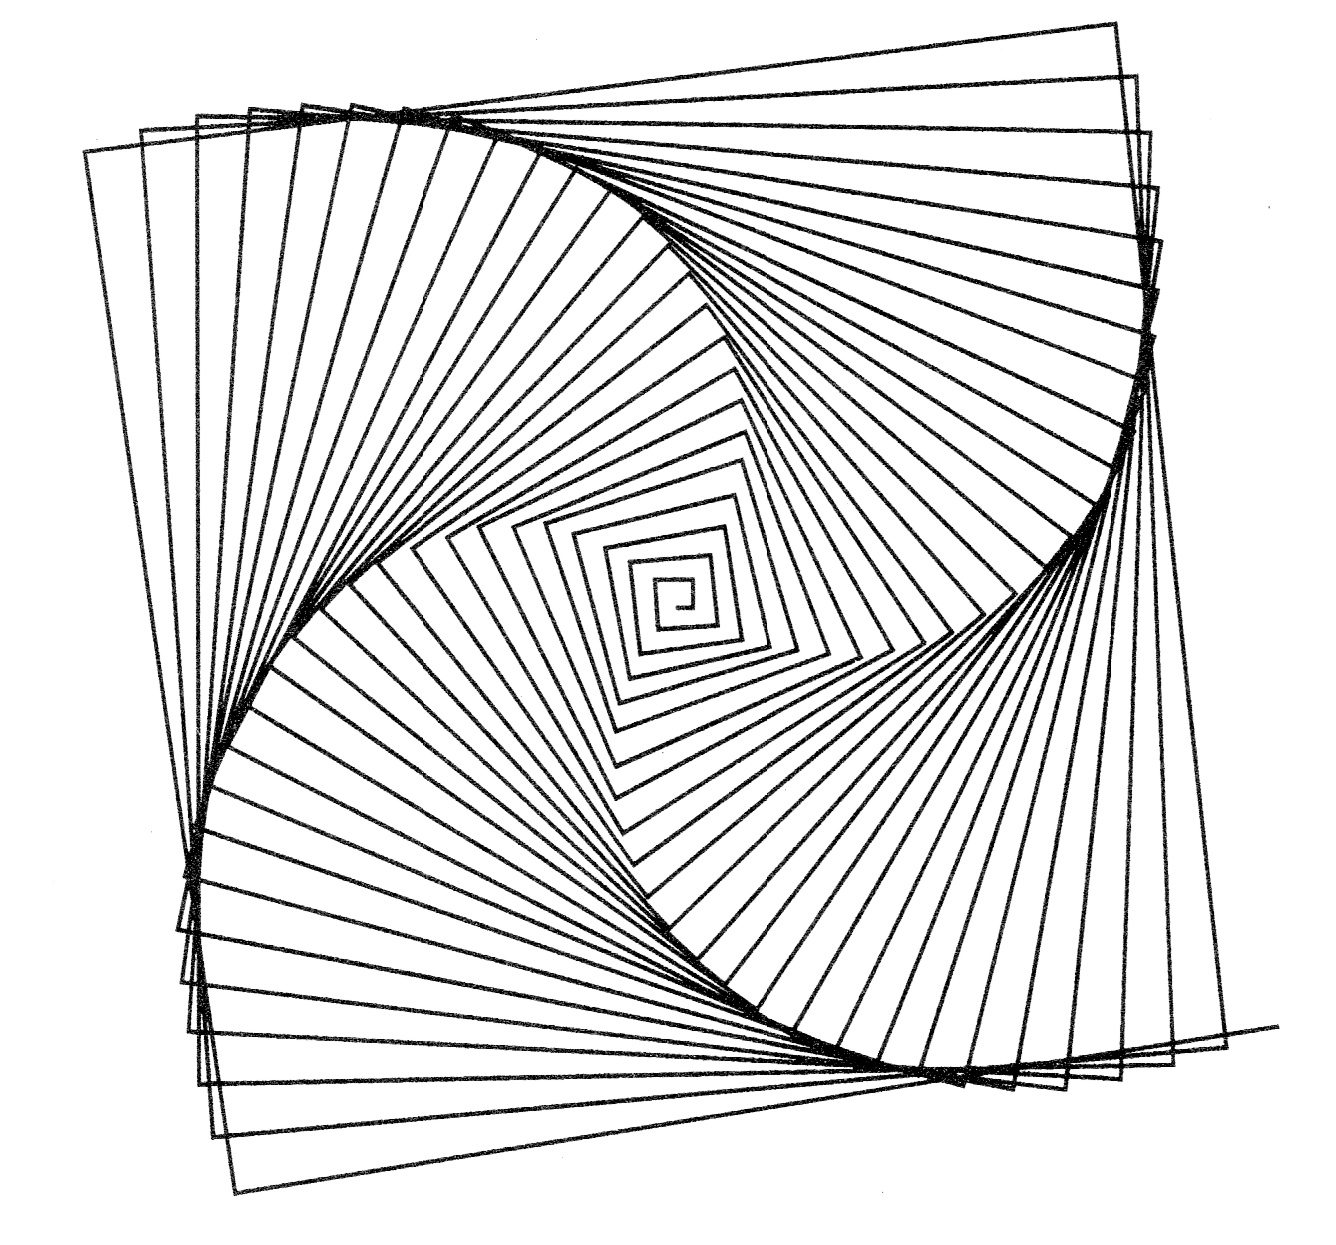
\includegraphics[height=40mm ,width=40mm ]{Imatges/Preface2.jpg}

\paragraph{Posar en joc l'abstracció.} La tercera part introdueix la necessitat de l'abstracció, és a dir, de mètodes
o procediments que poden ser reutilitzats per programes diferents. El concepte 
més difícil que s'introdueix és la idea de composar nous mètodes a partir de mètodes
ja existents per resoldre problemes més complexos. Proposaré diversos 
experiments no trivials, com ara dibuixar rectangles d'or. També introduirem
tècniques i eines per depurar (\textit{debug}) programes.

%% Aqui va la figura dels rectangles d'or
\vspace{5mm}
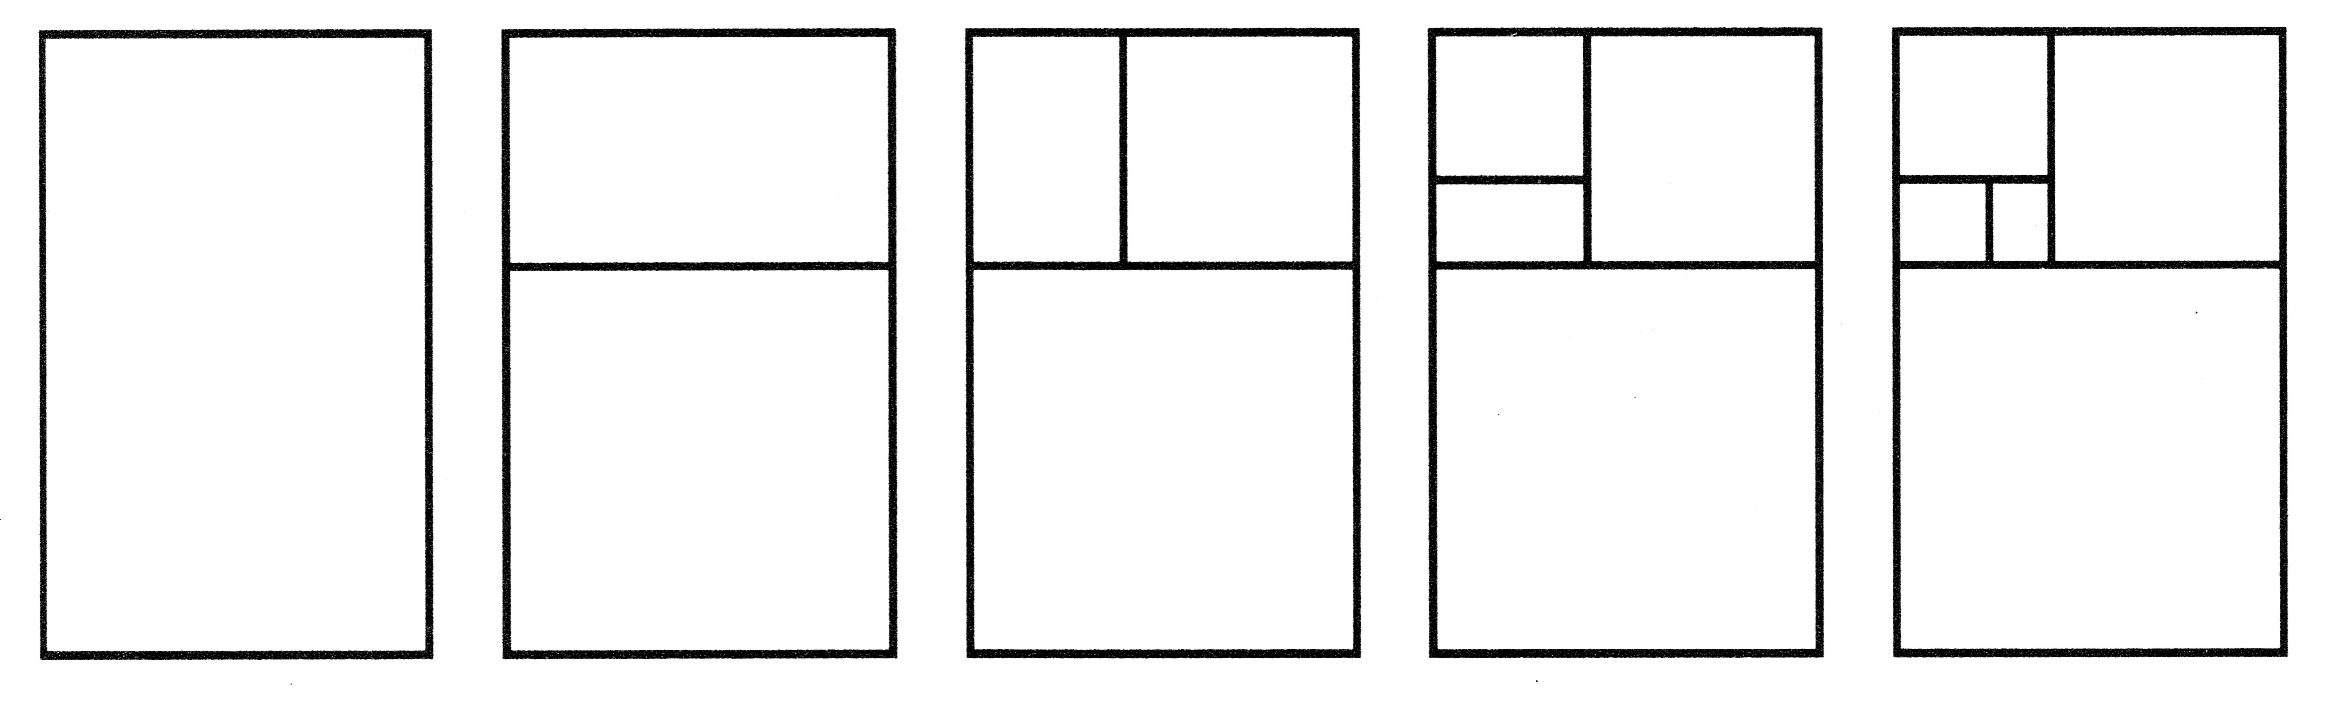
\includegraphics[height=30mm ,width=100mm ]{Imatges/Preface3.jpg}

\paragraph{Condicionals.} La quarta part introdueix les nocions de condicional, bucle condicional i 
expressió booleana, totes fonamentals per a la programació. Aquesta part 
explica també el concepte de referència en un espai bidimensional i altres
tipus de comportaments robòtics. Finalment, es presenten maneres d'utillitzar
els robots per simular el comportament d'animals simples.

%% Aqui va la figura dels comportaments d'animals
\vspace{5mm}
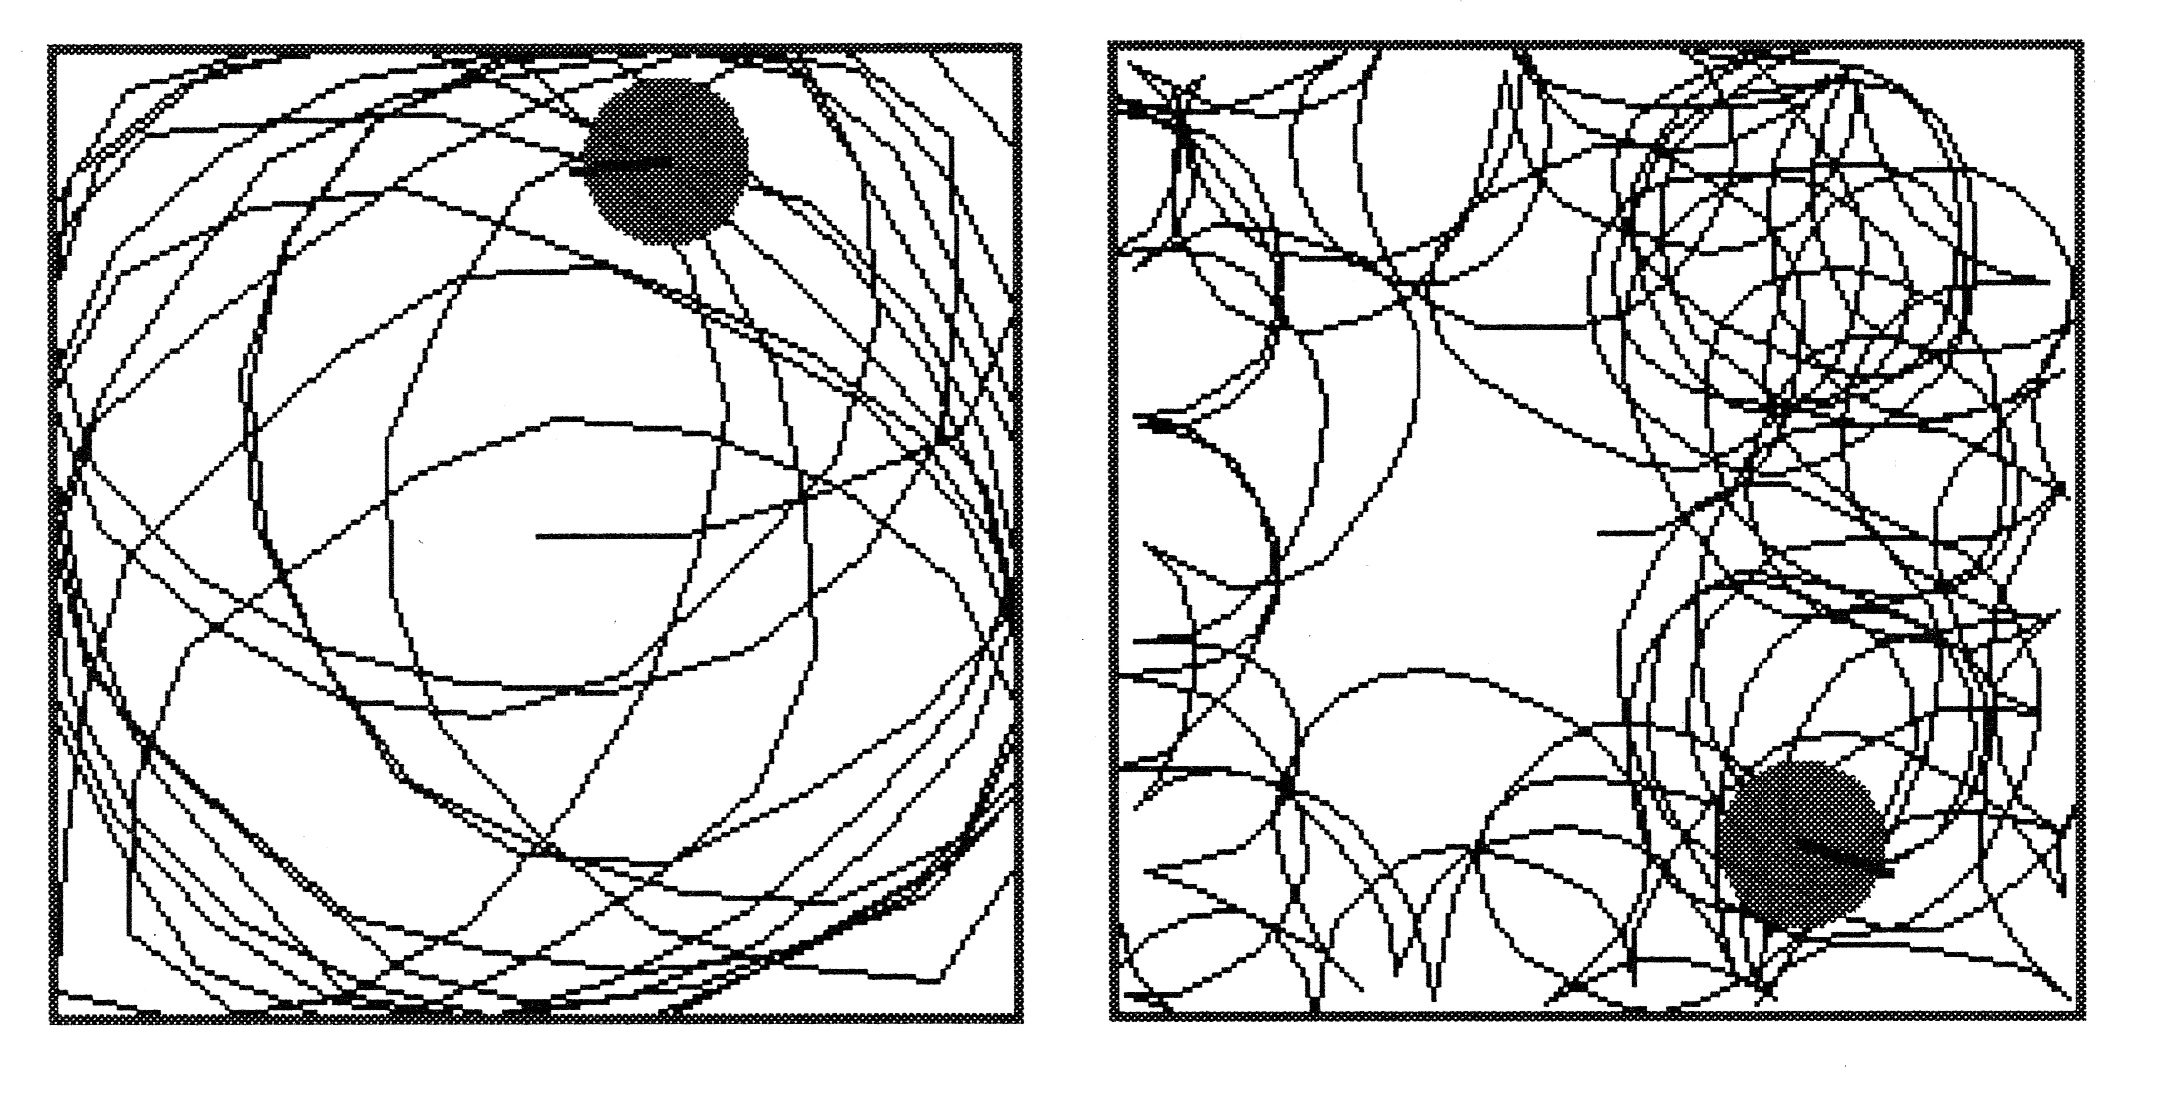
\includegraphics[height=45mm ,width=90mm ]{Imatges/Preface4.jpg}

\paragraph{Altres Mons Squeak.}
La cinquena part presenta dos entorns de programació força entretinguts que estan
disponibles en Squeak: el sistema d'\textit{scripting} gràfic \textsf{eToy} i l'entorn
\textsf{3D Alice}.

\section*{Per quina raó Squeak i Smalltalk?}

Podeu preguntar-vos perquè, d'entre el gran nombre de llenguatges de 
programació existents avui dia, he triat Smalltalk. Els he triat per les seguents raons:

\begin{itemize}
\item Smalltalk és un llenguatge molt potent. Podeu construir sistemes molt
complexos en un llenguatge que és simple i uniforme.
\item Smalltalk va ser dissenyat com un llenguatge per a l'ensenyament. Va inspirar-se
en Logo i en Lisp, i va influenciar fortament
llenguatges com Java o C\#. Tot i així, aquests llenguatges són massa complexos 
per a una primera aproximació a la programació. A més, han perdut la bellesa de
la simplicitat d'Smalltalk. 
\item Smalltalk és un llenguatge tipat dinàmicament i això torna irrellevants una
sèrie de qüestions relacionades amb tipus i coerció de tipus que són difícils
d'explicar i de poc interès pels neòfits.
\item Amb Smalltalk només cal aprendre conceptes clau, essencials, que es poden
trobar en tots els llenguatges de programació. Així, puc 
concentrar-me a explicar els conceptes importants sense haver de tractar altres
aspectes més difícils i poc atractius dels llenguatges més complexos.
\item Squeak és un potent entorn multimèdia, de manera que després de llegir 
aquests llibres hom podrà construir programes en un entorn 
realment ric.
\item Squeak està disponible gratuïtament i es pot executar en totes les 
plataformes principals. I hauria de ser fàcilment portable a altres
plataformes del futur.
\item Squeak és popular. Per exemple, a 
Espanya\footnote{\emph{Nota del traductor}: Ducasse es refereix a la 
utilització que es fa d'Squeak a Extremadura. \\ Veure \textsf{http://squeak.educarex.es/squeakpolis}} 
s'utilitza a les escoles, on s'executa en uns 80.000 ordinadors.
\end{itemize}

 

\mainmatter 

\renewcommand{\chaptermark}[1]{
\markboth{\fontfamily{phv}\selectfont  \upshape \chaptername
\ \thechapter.\ #1}{\fontfamily{phv}\selectfont  \upshape \chaptername
\ \thechapter.\ #1}
}

\part{Començar}

\chapter{Instal·lació i creació de robots}
\label{cap1}
  
Poseu en marxa el vostre cronòmetre! En cinc minuts, l'\textit{entorn} de joc dels robots, que utilitzareu en aquest llibre, estarà executant-se i preparat per a que us divertiu fent-lo servir. En aquest capítol aprendreu com instal·lar l'entorn, a conèixer-ne les diferents parts i començareu a interactuar amb els robots que viuen en aquest entorn. Aprendreu com programar aquests robots per aconseguir que realitzin tasques interessants tot enviant-los \textit{missatges}.

Així, comencem instal·lant l'entorn i preparant-nos pels reptes que vindran. Si el vostre entorn ja està instal·lat, apagueu el cronòmetre, salteu la primera secció i aneu directament a les seccions següents, que fan un resum de l'entorn. Després que hagueu adquirit una mica de soltura amb els robots als capítols~\ref{cap2}, \ref{cap3} i~\ref{cap4}, entraré  més en detall sobre la utilització de l'entorn al capítol~\ref{cap5}.

\section{Instal·lar l'entorn}
\index{entorn!instal·lar}
\index{instal·lació!en sistemes Windows i Macintosh}
\index{Squeak!instalacio@instal·lació|(}
L'entorn utilitzat en aquest llibre ha estat desenvolupat per executar-se sobre Squeak. Squeak és un entorn multimèdia \emph{open source}  ric i potent escrit completament en Smalltalk i disponible gratuïtament per a la majoria de sistemes operatius a \textsf{http://www.squeak.org}. Tingueu en compte, però, que no utilitzarem la distribució Squeak per defecte. Farem servir una distribució que hem preparat per utilitzar amb aquest llibre. Es pot aconseguir de l'editorial que el publica\footnote{\emph{Nota del Traductor}: Es refereix al llibre original, publicat en anglès per Apress.},  \textsf{http://www.apress.com}, a la secció de \emph{downloads}.\index{Squeak!downloading@\emph{downloading}} \index{llocs web!Squeak}

Squeak s'executa exactament igual en totes les plataformes. Malgrat això, per fer-vos la vida més fàcil, he preparat diversos fitxers comprimits que depenen de la plataforma. El principi és exactament el mateix en un Mac, un PC, o qualsevol altra plataforma. Les úniques diferències són les eines que cal fer servir per descomprimir fitxers i la manera en què Squeak arrenca. Un cop s'ha obtingut un fitxer anomenat \textsf{Ready[Mac/PC].zip}, cal descomprimir-lo i arrosegar el fitxer anomenat \textsf{Ready.image} (Mac) o \textsf{Ready} (PC) sobre l'aplicació \textsf{Squeak} i ja està! El fitxer \textsf{Ready}[\textsf{.image}] conté l'entorn complet utilitzat en aquest llibre. Tingueu en compte que pot ser que els fitxers no es diguin exactament igual, però això no té importància a l'hora de fer-los funcionar\footnote{\emph{Nota del Traductor}: Recordeu que hi ha una versió en català de l'entorn. Només cal utilitzar els fitxers \textsf{ReadyPC.zip} o \textsf{ReadyMac.zip} del servidor mencionat al principi del llibre. Tota la resta de l'explicació que fa el capítol és vàlida, tot i que al final obtindrem la imatge en català. Aquesta és la imatge que utilitzarem en aquest llibre traduït}.

\subsection{Instal·lació en un Macintosh}
\index{Macintosh!instal·lar Squeak en un}
Per instal·lar l'entorn en un Macintosh hauríeu de tenir un fitxer ZIP anomenat \textsf{ReadyMac.zip}. Usualment, fent doble clic sobre la icona s'hauria d'executar el programa de descompressió corresponent, com per exemple l'\emph{Stuffit Expander}. Un cop aquest arxiu ha estat descomprimit, hauríeu d'obtenir sis fitxers, tal com es mostra en la figura~\ref{fig0101}. Hauríeu d'identificar dos fitxers: el fitxer anomenat \textsf{Ready.image} i el fitxer executable \textsf{Squeak.app} (l'extensió \textsf{.app} pot no aparèixer)

\begin{figure}[h]
\begin{center}
\includegraphics[height=50mm ,width=82mm ]{Imatges/CarpetaReadyMac.png}
\end{center}
\caption{Els fitxers preparats per ser utilitzats pel Macintosh. \emph{Esquerra}: el fitxer ZIP. \emph{Dreta}: Els fitxers descomprimits.}
\label{fig0101}
\end{figure}

\subsection{Instal·lació en Windows}
\index{Windows!instal·lar Squeak a}
Per instal·lar l'entorn sobre windows, hauríeu de tenir un fitxer ZIP anomenat \textsf{ReadyPC.zip}. Un cop es descomprimeix aquest fitxer, hauríem d'obtenir vuit fitxers, tal com es veu a la figura~\ref{fig0102}.  Hauríeu d'identificar dos fitxers: el fitxer anomenat \textsf{Ready} i el fitxer executable \textsf{Squeak}

\begin{figure}[h]
\begin{center}
\includegraphics[height=50mm ,width=127mm ]{Imatges/CarpetaReadyPC.PNG}
\end{center}
\caption{Els fitxers preparats per ser utilitzats per un PC. \emph{Esquerra}: el fitxer ZIP. \emph{Dreta}: Els fitxers descomprimits.}
\label{fig0102}
\index{Squeak!instalacio@instal·lació|)}
\end{figure}

\section{Obrir l'entorn}
\index{entorn!obrir|(}
Per obrir l'entorn, arrossegueu el fitxer \textsf{Ready}[\textsf{.image}]  sobre la icona del fitxer executable \textsf{Squeak}[\textsf{.app}], com veieu a la figura~\ref{fig0103}. Hauríeu d'obtenir l'entorn tal com es mostra a la figura~\ref{fig0104}. Si no obteniu aquest entorn, llegiu la secció ``Problemes amb la Instal·lació'' que trobareu al final d'aquest capítol.\index{Macintosh!obrir l'entorn en un}  \index{Windows!obrir l'entorn a}

\begin{figure}[h]
\begin{center}
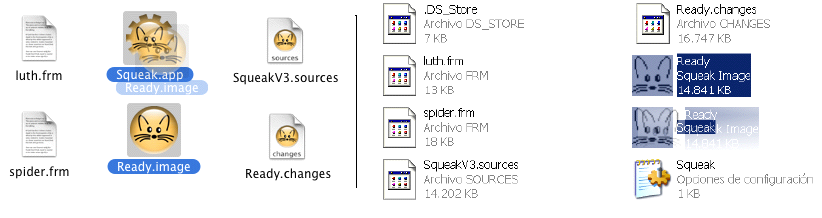
\includegraphics[height=35mm ,width=140mm ]{Imatges/fusio.png}
\end{center}
\caption{Arrosegar el fitxer imatge i deixar-lo anar sobre el fitxer executable \textsf{\upshape Squeak}, l'entorn s'obre en un Mac (esquerra) o en un PC (dreta).}
\label{fig0103}
\end{figure}

\newpage

\begin{figure}[h!]
\begin{center}
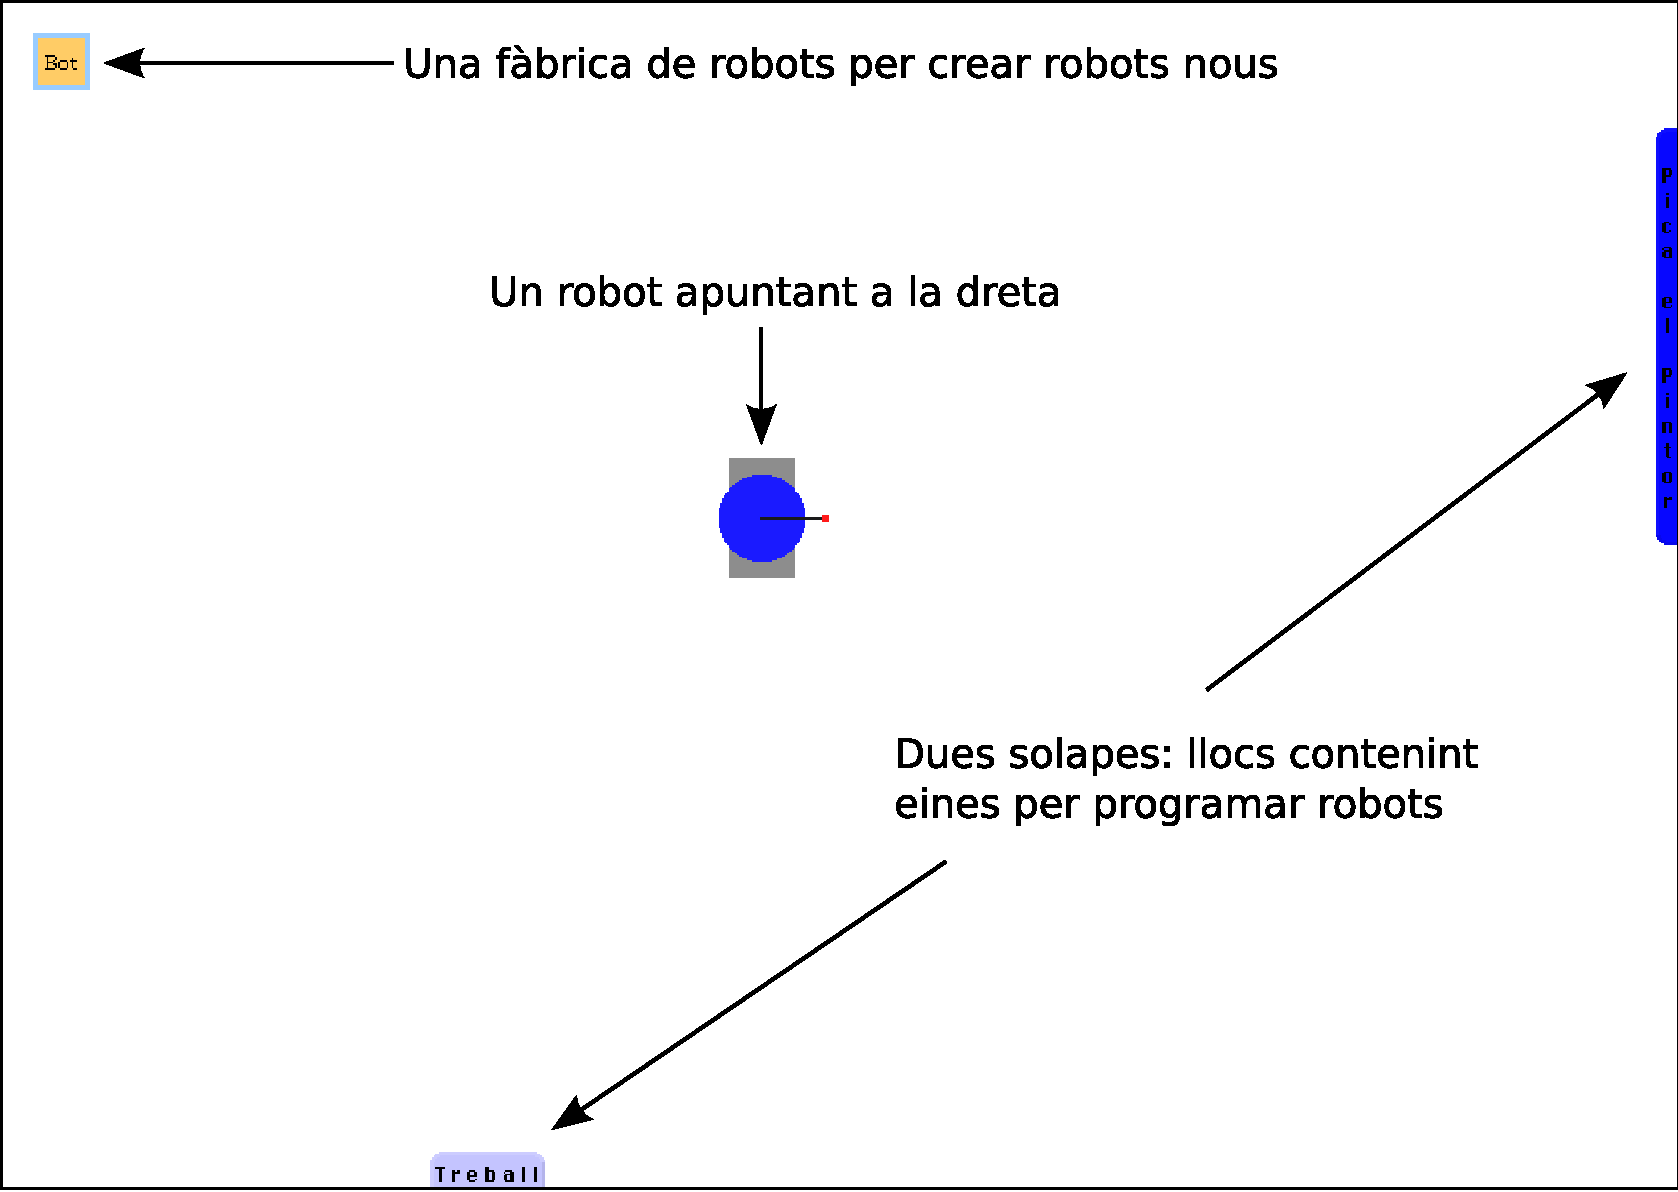
\includegraphics[scale=0.4]{Imatges/figura1-4}
\end{center}
\caption{L'entorn preparat per ser utilitzat.}
\label{fig0104}
\end{figure}

\vspace*{5mm}

\begin{figure}[h!]
\begin{center}
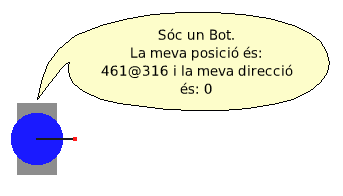
\includegraphics[height=45mm ,width=79mm ]{Imatges/figura1-5.png}
\end{center}
\caption{Poseu el ratolí sobre un robot per fer aparèixer una bafarada amb informació sobre el robot}
\label{fig0105}
\end{figure}

\newpage

\subsection{Ajuts a la instal·lació}
\index{instal·lació!ajuts a la}
L'entorn pot ser obert simplement fent doble clic sobre el fitxer imatge. Això, però, té alguns desavantatges: Heu d'identificar l'aplicació \textsf{Squeak} i de vegades una altra aplicació pot interferir i provar d'utilitzar el fitxer d'imatge. És més, podeu tenir problemes si teniu diverses instal·lacions de diferentes versions d'Squeak. Així doncs, us suggereixo que sempre obriu l'entorn arrossegant la imatge sobre l'aplicació \textsf{Squeak} o un algun àlies de l'aplicació.
Penseu que si no teniu prou espai per a la instal·lació en el disc dur, podeu fer servir un àlies pel fitxer \textsf{SqueakV3.sources}, que es pot compartir entre diverses instal·lacions.

\vspace{3mm}
\noindent
\rule{\textwidth}{2pt}
\noindent
\textbf{Important!} Per arrencar l'entorn, arrossegueu el fitxer \textsf{Ready} (amb la extensió \textsf{.image}  pel Mac) sobre l'aplicació \textsf{Squeak}. \\
\noindent
\rule{\textwidth}{2pt}

\section{Primeres interaccions amb un robot}
\index{entorn!obrir|)}
\index{robots!identificar dins l'entorn}
Un cop heu obert l'entorn arrossegant el fitxer anomenat \textsf{Ready}[\textsf{.image}]  sobre l'aplicació \textsf{Squeak}  tal com heu vist abans, l'entorn que s'obté hauria d'assemblar-se al que podem veure a la figura~\ref{fig0104}.

L'entorn està compost d'una fàbrica de robots i dues solapes. Una solapa és com una capsa que conté eines per programar. No les necessitareu de seguida, de manera que ja les descriuré en un altre capítol, més endavant. Hauríeu de veure un petit robot blau al mig de la pantalla. Aquest no és un robot fet de cables i metall sinó un programa-robot, vist des de dalt, apuntant cap al cantó dret de la pantalla. Un robot és una rodona blava; té dues rodes i un petit cap de color vermell que apunta en la seva direcció actual. Més endavant, si aneu seguint el llibre, enviareu ordres als robots. Aquestes ordres s'anomenen \emph{missatges}, i direm que els robots \emph{executen} aquests missatges. \index{entorn!components del} \index{solapa!definició de}

Poseu el ratolí sobre el robot i espereu un segon. Apareix una bafarada amb alguna informació sobre el robot, com la seva posició actual i la seva direcció, tal com veiem en la figura~\ref{fig0105}. Com que els monitors poden ser de diferents mides i resolucions, la posició del vostre robot no ha de ser necessàriament la de la figura. \index{bafarada, mostrant missatges mitjançant els} \index{entorn!identificar robots} \index{robots!obtenir informació sobre}

\subsection{Enviar missatges al robot}
\index{missatges!exemples de}
\index{missatges!enviar als robots|(}
\index{robots!enviar missatges a}
Podeu interactuar directament amb un robot fent clic amb el botó esquerre del ratolí sobre el robot (o fent només un clic amb un ratolí d'un sol botó). Una bafarada de missatges apareix, tal com veiem a la part esquerra de la figura~\ref{fig0106}. En aquesta bafarada hi podem escriure missatges que s'enviaran al robot. Després d'escriure el missatge, l'envieu al robot prement la tecla \emph{return}, i el robot aleshores l'executa.

\newpage

\begin{figure}[h!]
\begin{center}
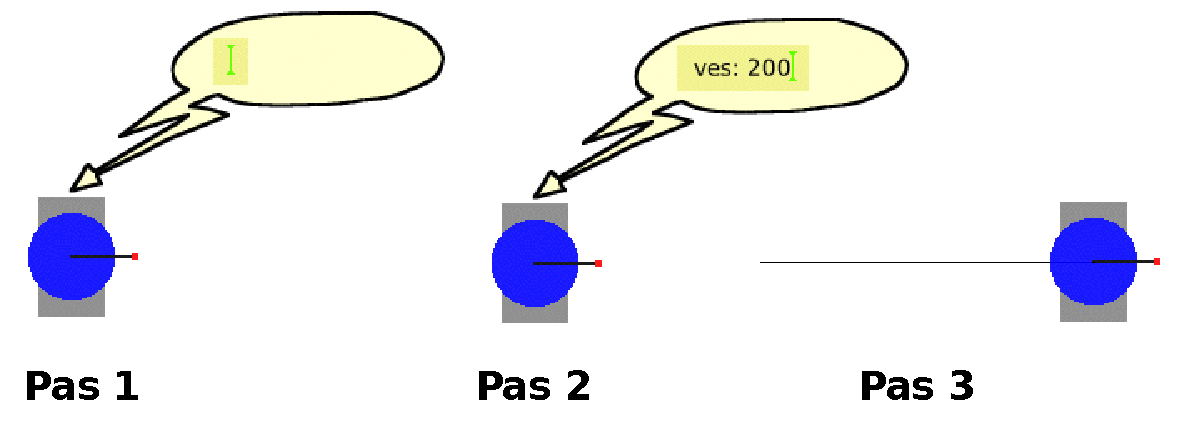
\includegraphics[scale=0.75]{Imatges/figura1-6}
\end{center}
\caption{\emph{Pas 1}: Fent clic amb el botó esquerre del ratolí sobre el robot, apareix una bafarada de missatges. \emph{Pas 2}: Podeu escriure un missatge al robot per fer-lo moure 200 píxels endavant, i  prémer return. \emph{Pas 3}: El robot executa el missatge; s'ha mogut, deixant un rastre a la pantalla en forma de línia.}
\label{fig0106}
\end{figure}

\vspace*{10mm}

\begin{figure}[h!]
\begin{center}
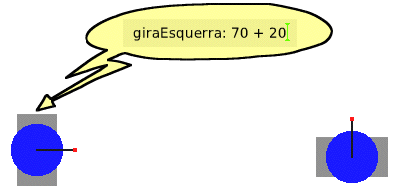
\includegraphics[height=45mm ,width=93mm ]{Imatges/figura1-7.png}
\end{center}
\caption{\emph{Esquerra}: Enviar un missatge compost. \emph{Dreta}: El missatge fa que el robot giri a l'esquerra 90 graus.}
\label{fig0107}
\end{figure}

\newpage

Per exemple, si hom escriu el missatge \textsf{ves: 200} seguit de \emph{return}, el robot rep l'ordre de desplaçar-se endavant 200 píxels en la seva direcció actual. Si hom escriu el missatge \textsf{giraEsquerra: 20 + 70}, s'està ordenant al robot que giri cap a l'esquerra (en el sentit contrari al de les agulles del rellotge) \textsf{20 + 70 = 90} graus, tal com veiem a la figura~\ref{fig0107}. Aquest segon missatge és més complicat que l'anterior, ja que el valor que representa el nombre de graus que el robot ha de girar és en ell mateix un missatge (tal com explicarem ben aviat), és a dir,  \textsf{20 + 70}. Anomenarem a aquests missatges \emph{missatges compostos}. Quan s'envia el missatge \textsf{color: Color verd}, el robot canvia de color, tal com veiem a la figura~\ref{fig0108} (us heu d'imaginar el color verd si la imatge és en escala de grisos). \index{missatges compostos!definició de} \index{missatges compostos!exemples de|(} \index{missatges compostos!enviar}\index{ves missatge!efecte de} \index{giraEsquerra: missatge, efecte de}

\begin{figure}[h]
\begin{center}
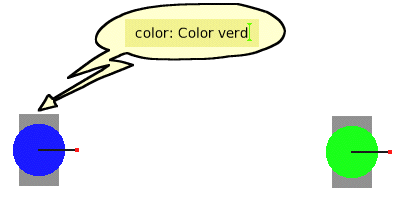
\includegraphics[height=45mm ,width=86mm ]{Imatges/figura1-8.png}
\end{center}
\caption{\emph{Esquerra}: S'ordena al robot canviar el seu color a verd. \emph{Dreta}: El color ha canviat.}
\label{fig0108}
\end{figure}

Pot ser que no entengueu el format dels missatges que acabem de presentar. Alguns poden semblar una mica complicats. De fet, \textsf{color: Color verd} és un altre missatge compost. Explicaré més tard com podeu construir els vostres propis missatges. Ara per ara, simplement escriviu els missatges que anirem presentant de manera que us aneu familiaritzant amb l'entorn dels robots. Si voleu repetir un missatge que ja havíeu escrit, no cal que el torneu a escriure. Utilitzeu les tecles \emph{amunt} i \emph{avall} per navegar pels missatges que ja havíeu enviat al robot. En propers capítols, aprendreu pas a pas tots els missatges que un robot entén, i a més, aprendreu com definir nous comportaments per als vostres robots.\index{color, missatges!efecte de} \index{robots!interactuar amb}

\noindent
\rule{\textwidth}{2pt}
\noindent
\textbf{Nota} Per interactuar amb un robot, feu clic al damunt, escriviu un missatge i premeu la tecla \emph{return}\\
\noindent
\rule{\textwidth}{2pt}

\section{Crear un nou robot}
\index{missatges compostos!exemples de|)}
\index{robots!crear}
\index{missatges!enviar als robots|)}
\index{nou, missatge; efecte de}
\index{fabriques de robots@fàbriques de robots!enviar missatges a les}
L'entorn ja conté un robot; ara, però, us ensenyaré com crear nous robots. Si no esteu satisfets tenint només un robot, podeu crear-ne un de nou enviant el missatge adequat a la \emph{fàbrica} de robots. Una fàbrica de robots és representada gràficament per una caixa  de color taronja envoltada per una caixa de color blau cel, al mig de la qual hi ha escrita la paraula \textsf{Bot}, com veieu a la figura~\ref{fig0109} . En l'argot d'Squeak, i en general en l'argot de la programació orientada a objectes, una fàbrica de robots és anomenada una \emph{classe}. Les classes (fàbriques que produeixen \emph{objectes}, com els robots) tenen un nom que comença per majúscula. Per tant aquesta és la classe \textsf{Bot}, i no \textsf{bot}.

\begin{figure}[h]
\begin{center}
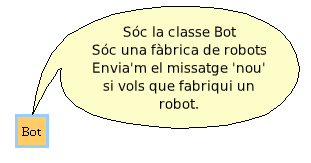
\includegraphics[height=45mm ,width=86mm ]{Imatges/figura1-9.png}
\end{center}
\caption{En l'argot d'Squeak, una fàbrica de robots s'anomena una classe. Les classes produeixen objectes. La classe \textsf{\upshape Bot} produeix nous robots.}
\label{fig0109}
\end{figure}

De la mateixa manera que vau fer amb els robots, podeu interactuar amb una fàbrica de robots enviant-li missatges. El missatge per crear un robot nou és el missatge \textsf{nou}, com veieu a la figura~\ref{fig0110}. Cada nou robot, igual que el robot original, apunta cap a la dreta de la pantalla. Cada robot té una existència independent, i podeu enviar missatges a cadascun d'ells.\index{missatges!enviar a fàbriques de robots}

\begin{figure}[h]
\begin{center}
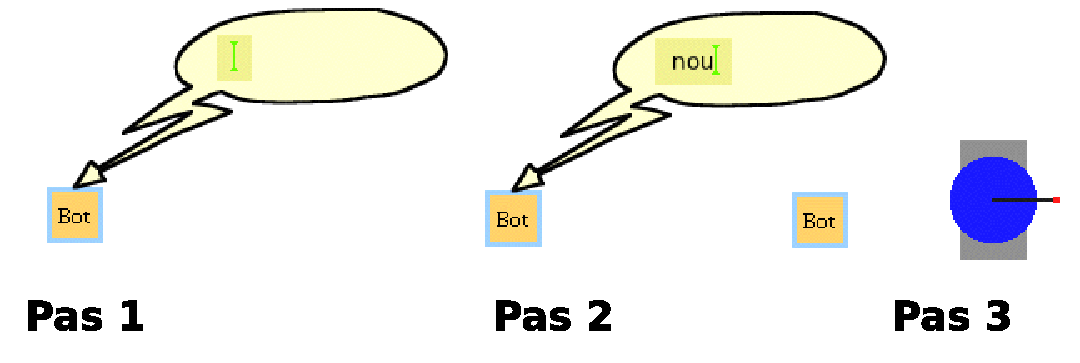
\includegraphics[scale=0.75]{Imatges/figura1-10}
\end{center}
\caption{\emph{Pas 1}: Comenceu a escriure un missatge.
 \emph{Pas 2}:  El missatge \textsf{\upshape nou} s'ha enviat a la fàbrica de robots.
\emph{Pas 3}: Com a resposta, la fàbrica ha creat un robot i us l'ha lliurat.}
\label{fig0110}
\end{figure}

\noindent
\rule{\textwidth}{2pt}
\noindent
Per crear un nou robot, envieu el missatge \textsf{nou} a la fàbrica de robots, que és la classe \textsf{Bot}. Quan es crea un robot, sempre apunta cap a l'\textsf{est}, és a dir, a la dreta de la pantalla.\\
\noindent
\rule{\textwidth}{2pt}

\section{Sortir i guardar}
\index{Squeak!sortir i guardar l'entorn}
\index{guardar l'entorn Squeak}
\index{entorn!sortir i guardar}
\index{sortir de l'entorn Squeak}
El fons de la finestra d'Squeak s'anomena el Món (\emph{World}). El Món té un menú que ofereix un cert nombre d'opcions. Per mostrar el menú del Món tan sols heu de fer clic amb el botó esquerre del ratolí sobre el fons de la finestra de l'entorn. Hauríeu d'obtenir un menú similar al que mostro a la figura 
~\ref{fig0111}. El darrer grup d'opcions són totes aquelles accions que podeu fer servir per sortir de l'entorn o guardar la vostra feina. \index{menus@menús, mostrar per Món} \index{Mon@Món (\emph{World}) menú!mostrar}

\begin{figure}[h]
\begin{center}
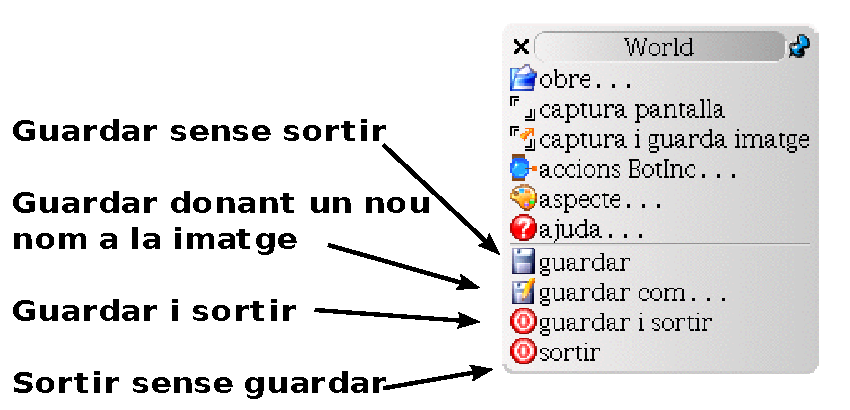
\includegraphics[scale=0.65]{Imatges/figura1-11}
\end{center}
\caption{El menú del Món (World) inclou accions per sortir i guardar.}
\label{fig0111}
\end{figure}

Seleccionar l'opció \textbf{sortir} senzillament tanca l'entorn sense guardar res de la vostra feina. El resultat és que la propera vegada que obriu l'entorn, estarà exactament en el mateix estat que la darrera vegada que el vau guardar. Seleccionar l'opció  \textbf{guardar} guarda tot l'entorn. La propera vegada que obriu l'entorn, estarà exactament en l'estat en que l'acabeu de guardar. Finalment, seleccionar l'opció \textbf{guardar com...}, l'entorn us preguntarà per un nom nou, i crearà dos fitxers nous amb aquest nom: un amb l'extensió \textsf{.image} i un altre amb l'extensió  \textsf{.changes}. Així és com jo vaig crear els fitxers \textsf{Ready}[\textsf{.image}] i \textsf{Ready.changes}. Per obrir l'entorn que heu guardat amb el nou nom, arrossegueu el fitxer amb el nou nom que té l'extensió \textsf{.image} sobre l'aplicació \textsf{Squeak}, tal com vau fer al començament per obrir l'entorn arrossegant el fitxer \textsf{Ready}[\textsf{.image}].

\section{Problemes amb la instal·lació}
\index{fitxer changes@fitxer \emph{changes}, resoldre problemes amb|(}
\index{fitxer imatge, resoldre problemes amb|(}
\index{fitxers!problemes amb|(}
\index{instal·lació!problemes amb|(}
\index{resoldre problemes d'instal·lació d'Squeak|(}
Algunes vegades les coses no van com podríem esperar, així que en aquesta secció donaré informació que us pot ajudar si teniu problemes amb la instal·lació. Primer, explicaré el rol dels principals fitxers que us heu trobat en descomprimir el fitxer descarregat.

Per executar l'entorn proporcionat amb aquest llibre, o amb qualsevol altra distribució Squeak, són necessaris quatre fitxers. Saber-ne alguna cosa pot ajudar-vos a resoldre alguns dels problemes que podríeu trobar.

\begin{itemize}
\item[] \textbf{Imatge i canvis}. El fitxer \textsf{Ready}[\textsf{.image}] , anomenat simplement el fitxer \emph{imatge}, i el fitxer \textsf{Ready.changes}, anomenat simplement el fitxer de \emph{canvis}, contenen informació sobre el vostre sistema Squeak actual. Aquests dos fitxers estan sincronitzats automàticament per Squeak i haurien de tenir els permisos d'escriptura habilitats. Cada cop que guardeu l'entorn, aquests dos fitxers es sincronitzen. No els hauríeu d'editar mai amb un editor de textos o canviar-los el nom manualment. Si voleu utilitzar diferents noms, utilitzeu l'opció \textbf{guardar com...} del menú del Món. Squeak crearà un nou parell de fitxers per a vosaltres.\index{Squeak!fitxers necessaris per a}
\item[] \textbf{Fonts}. El fitxer anomenat \textsf{SqueakV3.sources}, anomenat el fitxer dels \emph{fonts}, conté el codi font de part de l'entorn Squeak. No el necessitareu per estudiar aquest llibre, de manera que no proveu d'editar-lo manualment. Tot i així, aquest fitxer hauria d'estar sempre al mateix directori on teniu el fitxer imatge. \index{sources, fitxer; resoldre problemes amb} 
\item[] \textbf{Aplicació}. El fitxer executable \textsf{Squeak}[\textsf{.app}] per Mac, o \textsf{Squeak.exe} pel PC, és l'aplicació \textsf{Squeak}. Aquest fitxer és l'aplicació que s'executa quan esteu programant en Squeak. Hauria de tenir el permís d'execució habilitat. Aquest fitxer s'anomena l'aplicació \textsf{Squeak}. En l'argot de la informàtica, aquesta aplicació s'anomena una \emph{màquina virtual}, o MV. \index{fitxer de l'aplicació Squeak, resoldre problemes relacionats amb} \index{MV (màquina virtual), fitxer d'aplicació Squeak com a} \index{màquina virtual (MV), fitxer d'aplicació Squeak com a}
\end{itemize}

Recordeu que els fitxers d'imatge i de canvis haurien de tenir els permisos d'escriptura habilitats. Alguns sistemes operatius canvien les propietats dels fitxers a ``només lectura'' quan són copiats des de fonts externes. Si passa això, Squeak us avisa amb un missatge en anglès\footnote{\emph{Nota del Traductor}: L'Squeak amb què treballeu és un sistema força gran i, encara que pràcticament tot l'entorn BotsInc que fareu servir amb aquest llibre ha estat traduït, és molt possible que de tant en tant us apareguin missatges en anglès que pertanyen a l'entorn Squeak general.}, com el que us ensenyem a la figura~\ref{fig0112}. Si us surt aquest missatge, sortiu d'Squeak sense guardar, canvieu la propietat del fitxer per permetre l'escriptura, i torneu a obrir l'entorn. \index{aplicació (Squeak), fitxer de, resoldre problemes} \index{només lectura, identificar fitxers de}

\begin{figure}[h]
\begin{center}
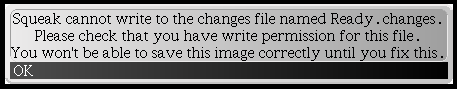
\includegraphics[height=20mm ,width=103mm ]{Imatges/figura1-12.png}
\end{center}
\caption{Aquest missatge apareix si la imatge (\textsf{\upshape Ready}[\textsf{\upshape .image}]) o el fitxer de canvis (\textsf{\upshape Ready.changes}) no tenen els permisos d'escriptura habilitats.}
\label{fig0112}
\end{figure}

Un altre problema que podeu trobar està relacionat amb el fitxer dels fonts \textsf{SqueakV3.sources}. Aquest fitxer, o un àlies referenciant-lo, hauria d'estar present al directori de la imatge. Si el fitxer no hi és, podeu trobar-vos amb el missatge (també en anglès) de la figura~\ref{fig0113}. Per resoldre aquest problema, creeu un àlies al fitxer \textsf{SqueakV3.sources} dins el directori que conté el fitxer de la imatge o simplement copieu el fitxer \textsf{SqueakV3.sources} dins aquest directori. No hauríeu de tenir aquest problema si esteu utilitzant la distribució feta per a aquest llibre.

\vspace*{5mm}

\begin{figure}[h]
\begin{center}
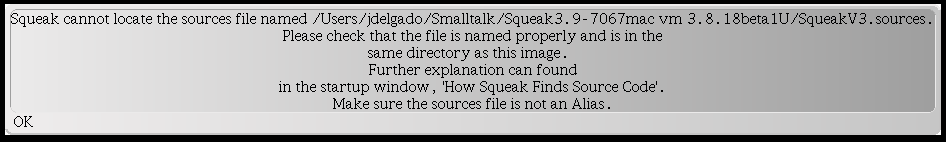
\includegraphics[height=20mm ,width=133mm ]{Imatges/figura1-13.png}
\end{center}
\caption{Missatge que indica que el fitxer dels fonts (\textsf{\upshape SqueakV3.sources}) no és al directori que conté el fitxer de la imatge.}
\label{fig0113}
\end{figure}
\index{fitxer changes@fitxer \emph{changes}, resoldre problemes amb|)}
\index{fitxers!problemes amb|)}
\index{instal·lació!problemes amb|)}
\index{resoldre problemes d'instal·lació d'Squeak|)}
\index{fitxer imatge, resoldre problemes amb|)}
\newpage

\section{Resum}

Per obrir l'entorn, arrossegueu el fitxer \textsf{Ready}[\textsf{.image}] o algun altre fitxer que hagueu guardat amb l'extensió \textsf{.image} dins l'aplicació \textsf{Squeak}.

\begin{itemize}
\item Per enviar un missatge a un robot, feu clic sobre el robot amb el botó esquerre del ratolí, escriviu el missatge i premeu \emph{return}.
\item Per crear un robot nou, envieu el missatge \textsf{nou} a la classe \textsf{Bot}, que és la vostra fàbrica de robots.
\item Quan es crea un robot, sempre apunta a l'\textsf{est}, és a dir, a la dreta de la pantalla.
\item Per obtenir el menú per guardar l'entorn feu clic en el fons de la finestra de l'entorn.
\end{itemize}

 \chapter{Un primer \emph{script} i les seves implicacions}
\label{cap2}

Enviar missatges als robots via interacció directa és una manera divertida i potent de programar-los, però és bastant limitada com a tècnica per escriure programes complicats. Per expandir els horitzons de les vostres possibilitats a l'hora de programar els robots, us ensenyaré la noció d'\emph{script}, que és una seqüència d'expressions, juntament amb els conceptes fonamentals i el vocabulari que necessitareu a la resta del llibre. Aquest capítol també servirà de mapa per als propers capítols, que introduiran en profunditat els conceptes breument presentats aquí. \index{scripts@\emph{scripts}!definició de}

Primer, us mostraré com enviar múltiples missatges al mateix robot, tot separant una seqüència de missatges amb punts i coma. Després aprendreu com escriure un \emph{script} utilitzant una eina anomenada \emph{Espai de Treball} (\emph{workspace}). Explicaré els elements diferents que composen un \emph{script} i mostraré alguns dels errors que hom pot cometre quan escriu un  programa.

\section{Utilitzar una cascada per enviar múltiples missatges}
\index{cascada|seealso{missatges}}
\index{cascada!enviar múltiples missatges amb}
\index{missatges!enviar amb cascades}
Imagineu que voleu fer que el robot que teniu en pantalla dibuixi un rectangle d'alçada 200 píxels i amplada 100 píxels. Per fer això, podríeu fer clic sobre el robot i començar a escriure el primer missatge, \textsf{ves: 100}, premeu la tecla \emph{return}, després feu clic i escriviu la segona expressió, \textsf{giraEsquerra: 90} i premeu la tecla \emph{return}, aleshores torneu a fer clic sobre el robot i escriviu \textsf{ves: 200} i així successivament. Ràpidament us adoneu que interactuar així amb el vostre robot és força tediós. Seria molt més convenient si poguéssiu escriure totes les instruccions de cop i executar-les totes només prement un botó.

De fet, podeu enviar múltiples missatges a un robot separant els missatges amb un punt i coma (\textsf{;}). Per enviar els missatges \textsf{ves: 100}, \textsf{giraEsquerra: 90} i \textsf{ves: 200} a un robot, escriviu-los separats per punts i coma, \textsf{ves: 100; giraEsquerra: 90; ves: 200} (veure figura \ref{fig0201}). Aquesta manera d'enviar múltiples missatges a un mateix robot s'anomena \emph{cascada de missatges} en l'argot d'Squeak. \index{ves missatge!dibuixar rectangles amb}

\begin{figure}[h]
\begin{center}
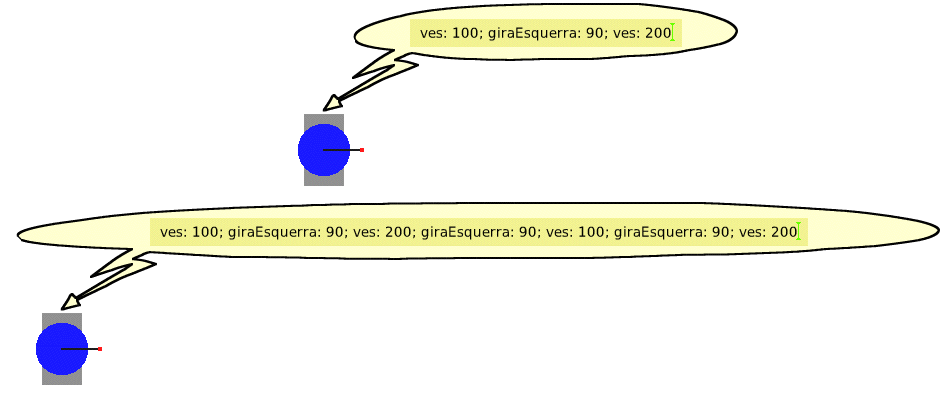
\includegraphics[height=60mm ,width=144mm ]{Imatges/figura2-1.png}
\end{center}
\caption{Podeu enviar d'una sola vegada diversos missatges a un robot utilitzant el caràcter punt i coma (\textsf{\upshape ;}).}
\label{fig0201}
\end{figure}

Malgrat tot, la tècnica d'escriure una cascada de missatges (vull dir, enviar a un robot múltiples missatges separats per punts i coma) no funciona bé per a programes complexos. De fet, fins i tot per dibuixar un simple rectangle, la seqüència de missatges ràpidament creix fins a ser massa llarga, com podeu veure en el segon missatge de la figura~\ref{fig0201}. I hi ha altres problemes. Per exemple, els programadors tenen en consideració aspectes com guardar una seqüència de missatges per executar-la més tard, o bé reutilitzar els seus missatges sense haver-los d'escriure altre cop. \index{rectangles!dibuixar}
Per aquestes raons, necessiteu alguna altra manera de programar robots. La primera manera que aprendreu és a escriure una seqüència de missatges, anomenada un \emph{script}\footnote{\emph{Nota del Traductor}: Per manca d'una traducció satisfactòria de la paraula anglesa ``script'' (que voldria dir ``petit programa''), la deixarem en anglés i en cursiva, per deixar clar que és un anglicisme.}, en un editor de text i demanar a l'entorn que executi el vostre \emph{script}.

\section{Primer \emph{script}}
\index{scripts@\emph{scripts}!escriure|(}
\index{editor de text Espai de Treball Bot!propietats}
\index{editor de text, utilitzar l'Espai de Treball Bot com a}
\index{Fes-ho tot (botó), efecte de|(}
L'entorn \textsf{Bot} proporciona un petit editor de text, anomenat l'\textsf{Espai de Treball Bot} (\emph{Bot Workspace}), que està pensat per a l'execució de programes. Feu clic a la solapa que trobareu a la part de sota, anomenada \textsf{Treball}. Per defecte conté un editor \textsf{Espai de Treball Bot}, com podeu veure a la figura~\ref{fig0202}.

\begin{figure}[h]
\begin{center}
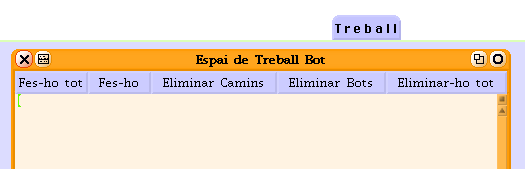
\includegraphics[height=35mm ,width=109mm ]{Imatges/figura2-2.png}
\end{center}
\caption{L' \textsf{\upshape Espai de Treball Bot} és un petit editor de text dedicat a l'execució de programes per als robots.}
\label{fig0202}
\end{figure}

Començarem escrivint un \emph{script} que dibuixa un rectangle, i després l'explicarem en detall (\emph{Script}~\ref{scr2-1}). \index{robots!crear picas}

\newtheorem{script}{Script}[chapter]
\begin{script} Creem el robot pica i el fem moure i girar
\noindent
\textsf{\upshape
\\
\\$|$ pica $|$\\
pica := Bot nou.\\
pica ves: 100.\\
pica giraEsquerra: 90.\\
pica ves: 200.\\
pica giraEsquerra: 90.\\
pica ves: 100.\\
pica giraEsquerra: 90.\\
pica ves: 200.\\
pica giraEsquerra: 90.\\
}
\label{scr2-1}
\end{script}

La figura~\ref{fig0203} mostra l'\emph{script} en un \textsf{Espai de Treball Bot} i el resultat de l'execució, obtingut prement el botó \textbf{Fes-ho tot}. Intenteu aconseguir el mateix resultat: escriviu l'\emph{script} i premeu el botó \textbf{Fes-ho tot}. He anomenat el robot \textsf{Pica} com a abreviatura de Picasso, ja que els nostres robots dibuixen, igual que ho feia el gran pintor espanyol.

El botó \textbf{Fes-ho tot} de l'\textsf{Espai de Treball Bot} executa \emph{tots} els missatges que conté l'espai de treball. Per tant, abans d'escriure un \emph{script}, assegureu-vos que no hi ha cap altre text escrit en l'espai de treball. És més, els ordinadors  i els llenguatges de programació no poden tractar ni el més mínim error, per obvi que sigui, així doncs, tingueu molta cura d'escriure el text exactament com està escrit en  l'\emph{Script}~\ref{scr2-1}. Per exemple, heu d'escriure la majúscula ``B'' de \textsf{Bot} a la segona línia, i heu d'acabar cada línia amb un punt (no cal posar el punt al final de la darrera línia, ja que els punts \emph{separen} missatges en Squeak. Tampoc cal un punt després de la primera línia, ja que no conté cap missatge). Ho ampliarem més endavant en aquest capítol. Podeu veure l'\emph{script} i el resultat d'executar-lo a la figura~\ref{fig0203}. \index{scripts@\emph{scripts}!escriure|)}

\begin{figure}[h]
\begin{center}
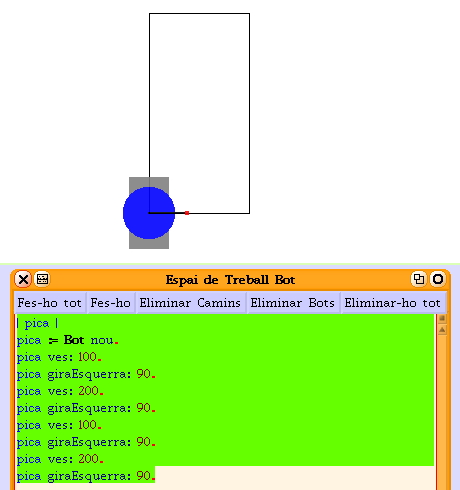
\includegraphics[height=110mm ,width=103mm ]{Imatges/figura2-3.png}
\end{center}
\caption{Un script executat utilitzant el botó \textbf{\upshape Fes-ho tot} de l' \textsf{\upshape Espai de Treball Bot} i el resultat de l'execució.}
\label{fig0203}
\end{figure}

\section{Squeak i Smalltalk}
\index{Smalltalk!significat de|(}
\index{Squeak!llenguatge@i el llenguatge de programació Smalltalk|(}
\index{Fes-ho tot (botó), efecte de|)} \index{expressions!relació amb els programes}
L'\emph{Script}~\ref{scr2-1} és molt senzill, tot i així és un autèntic programa informàtic. Un \emph{programa} és una llista d'\emph{expressions} que un ordinador pot executar. Per escriure programes necessitem llenguatges de programació, és a dir, llenguatges que permeten als programadors escriure instruccions que un ordinador pot ``entendre'' i executar.\index{programes!definició}

\subsection{Llenguatges de programació}
\index{llenguatges de programació}
Un llenguatge de programació ben dissenyat serveix per ajudar els programadors a expressar solucions als seus problemes. Per ajuda vull dir que el llenguatge hauria de, entre d'altres coses, facilitar l'expressió de la tasca a realitzar, proporcionar una execució eficient del codi del programa i confiança en el resultat, donar al programador la capacitat de demostrar que els seus programes són correctes, promoure la producció de codi llegible i facilitar als programadors fer canvis en les aplicacions. No existeix ni l'ideal, ni el ``millor'' llenguatge de programació que satisfaci totes aquestes propietats tan desitjables, i llenguatges de programació diferents estan millor adaptats a diverses tasques.

\subsection{Smalltalk i Squeak}
\index{llenguatge de programació orientat a objectes, Smalltalk com a}
Aquest llibre us ensenyarà com programar en el \emph{llenguatge de programació} Smalltalk dins de l'\emph{entorn de programació} Squeak. Un entorn de programació és un conjunt d'eines que els programadors utilitzen per desenvolupar aplicacions. Squeak conté un gran nombre d'eines útils: editors de text, exploradors de codi (\emph{code browsers}), depurador (\emph{debugger}), inspector d'objectes, compilador, \emph{widgets}, i molts altres. I això no és tot! En l'entorn Squeak podeu programar música, fitxers \emph{flash} animats, accedir a l'Internet, mostrar objectes 3D i molt més. Malgrat tot, abans no pugueu  programar aplicacions sofisticades heu d'aprendre alguns principis bàsics, i aquest és el propòsit d'aquest llibre.

Els programadors Squeak desenvolupen les seves aplicacions escrivint programes en el llenguatge de programació Smalltalk. Smalltalk és un llenguatge de programació \emph{orientat a objectes}. Altres llenguatges orientats a objectes són Java i C++, però Smalltalk és el més pur i el més senzill. Tal com suggereix el terme ``orientat a objectes'', aquest llenguatge de programació utilitza \emph{objectes}. Els objectes que són creats i utilitzats no són, naturalment, objectes reals sinó estructures lògiques, o objectes ``virtuals'', dins l'ordinador. Són anomenats objectes perque és útil pensar en aquestes estructures com a objectes reals manufacturats, com un robot, que és capaç d'entendre els missatges que rep i executar les instruccions que estiguin contingudes en aquests missatges. La raó de l'analogia amb els objectes és que podem utilitzar un robot, o una ràdio, o una càmara, sense conèixer la seva estructura interna. Només ens cal saber com utilitzar-los prement botons o enviant-los missatges via comandaments a distància.\index{fàbriques!relació amb objectes manufacturats}

D'on venen els objectes reals manufacturats? D'una fàbrica, naturalment. Les fàbriques d'objectes s'anomenen \emph{classes} en els llenguatges de programació orientats a objectes. Definir classes és una mica complicat, igual que la programació orientada a objectes en general, de manera que en aquest llibre introductori no us ensenyaré a definir classes. Enlloc d'això, el que acabarem fent és definir nous comportament pels nostres robots, i això ens donarà una bona base en els conceptes elementals de la programació.\index{classes!paper dins la programació orientada a objectes}

He triat Smalltalk com a llenguatge d'aquest llibre perquè és simple, uniforme i pur. Diem que és pur ja que a Smalltalk, \emph{tot} és un objecte que envia i rep missatges a i des d'altres objectes. Smalltalk és simple ja que només hi ha unes poques regles bàsiques, i és uniforme ja que aquestes regles s'apliquen sempre de manera consistent. De fet, Smalltalk va ser dissenyat originalment per ensenyar als neòfits a programar. Això, però, no significa que només puguem utilitzar Smalltalk per escriure aplicacions ``de joguina''. Hi ha aplicacions grans i complexes que han estat escrites en Smalltalk, com les aplicacions que controlen les màquines que fan els xips AMD que potser duu el vostre ordinador.

Una altra aplicació escrita completament en Smalltalk és l'entorn Squeak mateix. No us sembla interessant? Això significa que un cop entengueu bé el llenguatge Smalltalk, podeu modificar l'entorn Squeak per adaptar-lo a allò que vulgueu fer o simplement per aprendre més sobre el sistema. Així doncs, amb Smalltalk teniu un gran potencial a les vostres mans.

Espero que aquesta discussió sobre llenguatges de programació en general, i Smalltalk en particular, us hagi motivat prou com per voler aprendre a programar. Si us plau, sigueu conscients que aprendre a programar és com aprendre a tocar el piano o pintar a l'oli. No és simple, per tant no us desanimeu si trobeu algunes dificultats. Així com un pianista principiant no comença amb la sonata de Beethoven \emph{Waldstein Sonata}, i un pintor principiant no intenta reproduir el sostre de la capella sixtina de Michelangelo, un programador novell comença amb tasques senzilles. He dissenyat aquest llibre de manera que els continguts siguin introduïts en un ordre lògic i el que apreneu en cada capítol necessita del que heu après en capítols anteriors i us prepara per al que vindrà en capítols posteriors. \index{Smalltalk!significat de|)} \index{Squeak!llenguatge@i el llenguatge de programació Smalltalk|)}

\section{Programes, expressions i missatges}
\index{scripts@\emph{scripts}!relació amb les expressions}
Ara estem preparats per fer una ullada als detalls del vostre primer \emph{script}.

\subsection{Escriure i executar programes}
\index{programes!escriure i executar}
Quan vau escriure l'\emph{Script}~\ref{scr2-1}, vau escriure un text, constituint una sèrie d'expressions, i vau demanar a Squeak que l'executés tot prement el botó \textbf{Fes-ho tot}. Squeak va executar la seqüència d'expressions; això és, va transformar la representació textual del vostre programa en una forma comprensible per a l'ordinador,  i aleshores cada expressió va ser executada en sèrie. En aquest primer \emph{script}, executar la seqüència d'instruccions va crear un robot anomenat \textsf{pica} i \textsf{pica} va executar, un darrera l'altre, els missatges que li vau enviar.

Un programa en Squeak consisteix en una sèrie d'\emph{expressions} que han de ser executades per l'entorn Squeak. En aquest llibre anomenarem a aquesta seqüència un \emph{script}.\index{expressions!relació amb els programes}

\vspace{3mm}
\noindent
\rule{\textwidth}{2pt}
\noindent
\textbf{Important!} Un \emph{script} és una seqüència d'expressions.\\
\noindent
\rule{\textwidth}{2pt}
\vspace{3mm}

Un programa és com una recepta per a un pastís de xocolata. Una bona recepta descriu tots els passos que s'han de dur a terme en la seqüència correcta: barrejar els rovells d'ou amb sucre, fondre la cobertura de xocolata al bany maria, afegir mantega i remenar, muntar les clares i barrejar-ho tot, remenar-ho i posar-ho en un motllo per al forn; deixar coure al forn a 180 graus durant 30 minuts; deixar refredar i servir. I bon profit! Igualment, un programa informàtic descriu tots els passos en seqüència per aconseguir l'efecte desitjat: declarar (triar) el nom per a un robot; crear un robot amb aquest nom; dir-li al robot que es mogui 100 píxels; dir-li al robot que giri 90 graus; etcètera.

\subsection{Anatomia d'un \emph{script}}
\index{scripts@\emph{scripts}!analitzar|(}
Ja és hora d'analitzar el nostre primer \emph{script}, que reproduïm aquí com a \emph{Script}~\ref{scr2-2}.

\begin{script} 
\noindent
\textsf{\upshape
\\
\\$|$ pica $|$\\
pica := Bot nou.\\
pica ves: 100.\\
pica giraEsquerra: 90.\\
pica ves: 200.\\
pica giraEsquerra: 90.\\
pica ves: 100.\\
pica giraEsquerra: 90.\\
pica ves: 200.\\
pica giraEsquerra: 90.\\
}
\label{scr2-2}
\end{script}

Resumint, l'\emph{Script}~\ref{scr2-2} comença declarant que utilitzarà una \emph{variable} anomenada \textsf{pica} per referir-se al robot que crea. Un cop s'ha creat el robot i està associat amb la variable \textsf{pica}, l'\emph{script} li diu al robot que faci una seqüència específica de moviments a diferents llocs de la pantalla mentre gira 90 graus a l'esquerra després de cada moviment. Analitzem cada línia pas per pas. No us amoïneu si alguns conceptes com la noció de variable no queden clars. Tots ells seran explicats quan toqui, si no en aquest capítol, en un de posterior.

\begin{itemize}
\item[] \textsf{$\mid$ pica $\mid$}: Aquesta primera línia declara una \emph{variable}. Diu a Squeak que volem utilitzar el nom \textsf{pica} per referir-nos a un objecte. Penseu-ho com si diguéssiu a un amic: ``d'ara en endavant utilitzaré la paraula \textsf{pica} en les meves frases per referir-me al robot que estic a punt d'encarregar a la fàbrica de robots''. Aprendreu més sobre variables al capítol~\ref{cap8}.
\item[] \textsf{pica := Bot nou.}: Aquesta línia crea un robot nou enviant el missatge \textsf{nou} a la fàbrica (classe) de robots i associa el robot amb el nom \textsf{pica}, la variable declarada en el pas anterior. La paraula \textsf{Bot} requereix una B majúscula ja que és una classe, en aquest cas la classe (fàbrica) per produir robots.
\item[] \textsf{pica ves: 100.}: En aquesta expressió, el missatge \textsf{ves: 100} és enviat al robot anomenat \textsf{pica}. Aquesta línia pot ser entesa com: ``\textsf{pica}, mou-te 100 unitats pel monitor de l'ordinador''. És implícit en el missatge que el robot que rep un missatge \textsf{ves:} sap en quina direcció ha d'anar. De fet, un robot sempre apunta en alguna direcció, i quan rep un missatge \textsf{ves:}, sap que s'ha de moure en la direcció que està apuntant. Fixeu-vos que el missatge \textsf{ves:} acaba amb dos punts. Això vol dir que aquest missatge necessita informació addicional, en aquest cas una longitud. Per exemple, \textsf{ves: 100} diu que el robot s'hauria de moure 100 píxels. El nom del missatge és \textsf{ves:}.        
\item[]\textsf{pica giraEsquerra: 90.}: Aquesta línia li diu a \textsf{pica} que giri 90 graus a la seva esquerra (en sentit contrari a les agulles del rellotge). Aquesta línia és un altre missatge enviat al robot anomenat \textsf{pica}. El nom del missatge \textsf{giraEsquerra:} acaba en dos punts, i per tant cal donar informació addicional, en aquest cas un angle.   
\end{itemize}

\noindent
La resta de línies de l'\emph{script} són similars.\index{scripts@\emph{scripts}!analitzar|)}

\noindent
\rule{\textwidth}{2pt}
\noindent
\textbf{Important!} Qualsevol missatge que acaba amb dos punts indica que el missatge necessita informació addicional, com una longitud o un angle. Per exemple, el nom del missatge \textsf{giraEsquerra:} necessita un nombre que representi l'angle que el robot ha de girar en sentit contrari a les agulles del rellotge.\\
\noindent
\rule{\textwidth}{2pt}

\subsection{Sobre els píxels}
\index{pixels@píxels!significat de}
La unitat de distància en una pantalla d'ordinador s'anomena \emph{pixel}. Aquesta paraula va ser inventada cap al 1970 i és un acrònim de \emph{picture element}. Un pixel és la mida del punt més petit que es pot dibuixar a la pantalla d'un ordinador. La mida del pixel pot variar en funció del tipus de monitor. Es poden veure els píxels individuals mirant la pantalla amb una lupa.

\subsection{Expressions, missatges i mètodes}

Hem estat utilitzant els termes \emph{expressió} i \emph{missatge}. Ara és el moment de definir-los. També definirem el terme important \emph{mètode}.

\subsubsection*{Expressió}
\index{expressions!exemples de}
Una \emph{expressió} és qualsevol element amb significat d'un programa. Aquí teniu alguns exemples d'expressions:

\begin{itemize}
\item \textsf{$\mid$ pica $\mid$} és una expressió que declara una variable (més al capítol~\ref{cap8}). 
\item \textsf{pica := Bot nou.} és una expressió amb una operació, anomenada \emph{assignació}, que associa un valor amb una variable (veure capítol~\ref{cap8}). Aquí un robot, acabat de crear en haver enviat el missatge \textsf{nou} a la classe \textsf{Bot}, s'associa amb la variable \textsf{pica}.
\item \textsf{pica ves: 100.}  és una expressió que envia un missatge a un objecte. Aquesta expressió s'anomena \emph{enviament de missatge}. El missatge \textsf{ves: 100} és enviat a l'objecte anomenat \textsf{pica}.
\item \textsf{100 + 200} és també un enviament de missatge. El missatge \textsf{+ 200} és enviat a l'objecte \textsf{100}.
\end{itemize}

\subsubsection*{Missatge}
\index{missatges!exemples de|(}
Un \emph{missatge} és una parella composada pel nom del missatge, també anomenat \emph{selector del missatge}, i els possibles \emph{arguments} del missatge, que són els valors que l'objecte que rep el missatge necessita per poder executar-lo. Aquestes relacions estan il·lustrades a la figura~\ref{fig0204}. L'objecte que rep el missatge s'anomena el \emph{receptor del missatge}. Un missatge, juntament amb el receptor del missatge és el que anomenem un \emph{enviament de missatge}. Aqui teniu alguns exemples de missatges:

\begin{itemize}
\item A l'expressió \textsf{pica tornarInvisible}, el missatge \textsf{tornarInvisible} s'ha enviat a un receptor, en aquest cas un robot. Aquest missatge no té cap argument.
\item A l'expressió \textsf{pica ves: 100}, el missatge \textsf{ves: 100} ha estat enviat a un receptor, un robot anomenat \textsf{pica}. Està compost del selector del missatge \textsf{ves:} i un sol argument, el nombre \textsf{100}. Aquí, \textsf{100} representa la distància en píxels que el robot hauria de recòrrer. Fixeu-vos que els dos punts formen part del selector del missatge.
\item A l'expressió \textsf{33 between: 30 and: 50} el missatge  \textsf{between: 30 and: 50} està compost del selector del missatge  \textsf{between: and:} i de dos arguments  \textsf{30} i  \textsf{50}. Aquest missatge demana al receptor, aquí el nombre  \textsf{33}, si està entre dos valors, aquí els nombres \textsf{30} i  \textsf{50}.
\item A l'expressió \textsf{4 vegadesRepetir: [pica ves: 100]}, el missatge \textsf{vegadesRepetir: [pica ves: 100]}, que ha estat enviat al nombre \textsf{4}, es composa del selector del missatge \textsf{vegadesRepetir:}\footnote{\emph{Nota del Traductor} El mètode \textsf{between: and:} pertany al llenguatge Smalltalk general més que a l'entorn dels bots preparat per a aquest llibre. Per això no ha estat traduït. Hi ha, però, alguns mètodes d'Smalltalk que no pertanyen pròpiament a l'entorn dels bots que \emph{sí} que hem traduït, com per exemple \textsf{vegadesRepetir:}, que és \textsf{timesRepeat:} en Smalltalk. Això ho hem fet essencialment amb mètodes molt utilitzats i amb algunes estructures de control.} i de l'argument \textsf{[pica ves: 100]}. Aquest argument s'anomena un \emph{bloc}, que és una seqüència d'expressions (en aquest cas n'hi ha només una) dins d'un parell de claudàtors (més al capítol~\ref{cap7}).
\item A l'expressió \textsf{100 + 200}, el missatge \textsf{+ 200} es composa del selector de missatge \textsf{+} i un argument, el nombre \textsf{200}. El receptor és el nombre \textsf{100}.
\end{itemize}\index{missatges!exemples de|)}

\begin{figure}[h]
\begin{center}
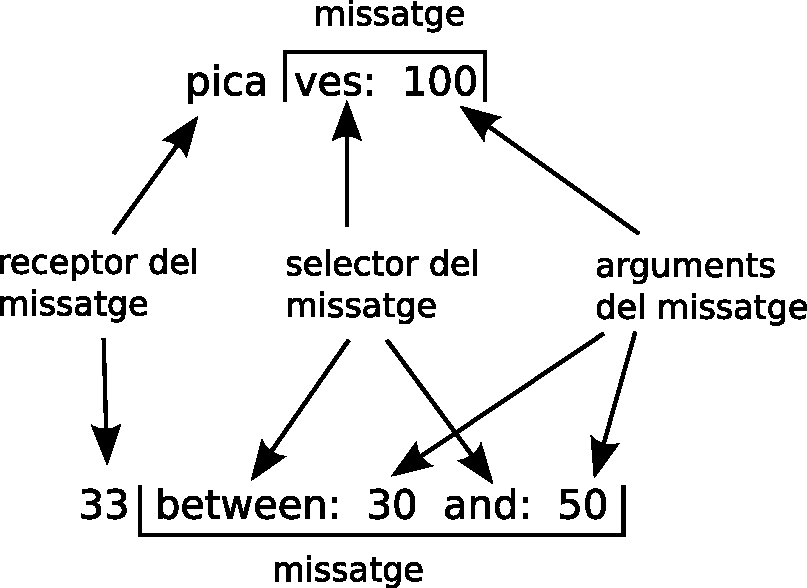
\includegraphics[scale=0.6]{Imatges/figura2-4}
\end{center}
\caption{Dos enviaments de missatges compostos d'un receptor del missatge, un nom de missatge (o selector del missatge) i uns arguments.}
\label{fig0204}
\end{figure}

\subsection{Separació de missatges}
\index{. (punt)!utilitzar en missatges i \emph{scripts}}
\index{punt (.)!utilitzar en missatges i \emph{scripts}}
Tal com hem dit abans, cada línia de l'\emph{Script}~\ref{scr2-1}, excepte la primera i l'última, s'acaba amb un punt. La primera línia no conté cap missatge. Una línia com aquesta s'anomena una \emph{declaració de variables} en argot informàtic. Així, podem fer la següent observació: cada missatge enviat ha de separar-se del següent amb un punt. Fixeu-vos que posar el punt després del darrer missatge és possible però no obligatori. Smalltalk ho accepta de les dues maneres. \index{declaració de variables, relació amb els missatges}

\vspace{3mm}
\noindent
\rule{\textwidth}{2pt}
\noindent
\textbf{Important!} Els enviaments de missatges haurien de separar-se amb un punt. El darrer enviament no requereix un punt. Aquí teniu quatre missatges separats per tres punts.

\noindent
\textsf{\upshape
\\
pica := Bot nou.\\
pica ves: 100.\\
pica giraEsquerra: 90.\\
pica ves: 100\\
}
\noindent
\rule{\textwidth}{2pt}

\noindent
\rule{\textwidth}{2pt}
\noindent
\textbf{Important!} El caràcter punt $.$ és un separador de missatges, de manera que no cal posar-ne un en acabar un enviament de missatge si no hi ha un altre enviament de missatge després. Per tant, no cal cap punt al final d'un \emph{script} o d'un bloc de missatges.\\
\noindent
\rule{\textwidth}{2pt}
 
\subsection{Mètode}
\index{metodes@mètodes!definició dels}
Quan un robot (o un altre objecte) rep un missatge, executa un \emph{mètode}, que és una mena d'\emph{script} amb nom. Més formalment, un mètode és una seqüència d'expressions amb nom que un objecte receptor executa en resposta a la recepció d'un missatge. Un mètode és executat quan un objecte rep un missatge del mateix nom que un dels seus mètodes. Per exemple, un robot executa el seu mètode \textsf{ves:} quan rep un missatge el nom del qual és \textsf{ves:}. Així doncs, l'expressió \textsf{pica ves: 224} provoca que el receptor del missatge, \textsf{pica}, executi el seu mètode \textsf{ves:} amb argument \textsf{224}, amb el resultat d'efectuar un moviment de 224 píxels endavant en la direcció actual. Més endavant explicarem com podeu definir nous mètodes per als vostres robots, ara per ara no cal saber-ho per començar a programar.

\subsection{Cascada}
\index{cascada!usos de}
Tal com vam mencionar en la primera secció d'aquest capítol, podeu enviar múltiples missatges a un robot separant-los amb punts i coma. Aquesta seqüència de missatges s'anomena una \emph{cascada}. També podeu utilitzar una cascada en un \emph{script} per enviar diversos missatges a un robot. L'\emph{Script}~\ref{scr2-3} és equivalent a l'\emph{Script}~\ref{scr2-2}, excepte que ara tots els missatges enviats al robot \textsf{pica} estan separats per punts i coma. Utilitzar cascades és pràctic quan voleu evitar escriure repetides vegades el nom del receptor dels múltiples missatges. Les cascades són útils ja que fan els \emph{scripts} més curts. Però aneu amb compte! Les dreceres poden donar-vos problemes si no mireu per on aneu; així doncs, assegureu-vos que realment voleu enviar tots els missatges al mateix receptor.

\newpage

\begin{script} 
\noindent
\textsf{\upshape
\\
\\$|$ pica $|$\\
pica := Bot nou.\\
pica \\
\hspace*{5mm}    ves: 100 ; giraEsquerra: 90 ; ves: 200 ; giraEsquerra: 90 ;\\
\hspace*{5mm}    ves: 100 ; giraEsquerra: 90 ; ves: 200 ; giraEsquerra: 90 .\\
}
\label{scr2-3}
\end{script}

\vspace{3mm}
\noindent
\rule{\textwidth}{2pt}
\noindent
\textbf{Important!} Per enviar múltiples missatges a un robot, utilitzeu el caràcter punt i coma ; per separar els missatges, seguint l'estructura \emph{unBot missatge1 ; missatge2}. Un exemple: \textsf{pica ves: 100 ; giraEsquerra: 90 ; ves: 200 ; giraEsquerra: 90}.\\
\noindent
\rule{\textwidth}{2pt}

\subsection{Crear nous robots}
\index{classes!obtenir nous objectes a partir de}
\index{robots!crear|(}
Per aconseguir un robot nou heu d'encarregar-lo a la fàbrica de robots. És a dir, heu d'enviar el missatge \textsf{nou} a la classe \textsf{Bot}. Això ja ho sabíem. És exactament el que vau fer en el capítol anterior quan vau fer clic sobre la capseta blava i taronja anomenada \textsf{Bot}, que representa la classe amb aquest nom, i vau escriure \textsf{nou} a la bafarada. A Squeak, sempre cal enviar missatges als robots, altres objectes o classes per interactuar amb ells. No hi ha cap diferència en el tractament, excepte que els objectes i les classes entenen diferents missatges. La feina de les classes és crear objectes. Un objecte no sap com crear altres objectes, de manera que obtenim un error si enviem el missatge \textsf{nou} a un robot. Les classes, per altra part, generalment no tenen colors i no saben moure's, per tant enviar missatges com \textsf{color} o \textsf{ves: 135} a una classe no té gaire sentit, i obtenim un error en fer-ho. Malgrat tot, en ambdós casos estem enviant missatges!

La classe \textsf{Bot} no és l'única fàbrica d'objectes en l'entorn Squeak. Hi ha altres classes, que entenen diferents missatges i utilitzen mètodes diferents per crear tipus diversos d'objectes. Per exemple, la classe \textsf{Color} fabrica colors (objectes-color). Retorna un color blau o verd en resposta al missatge \textsf{blau} o \textsf{verd}. En aquest llibre, quan calgui obtenir un objecte a partir d'una classe específica, ja us direm com fer-ho. \index{classe Bot!significat de} \index{objectes!obtenir de classes}\index{robots!crear|)}

\newpage

\noindent
\rule{\textwidth}{2pt}
\noindent
\textbf{Important!} Per obtenir un objecte nou a partir d'una classe, usualment s'envia el missatge \textsf{nou} a la classe\footnote{\emph{Nota del Traductor}: En realitat el missatge que usualment cal enviar a una classe per crear objectes dins de l'entorn Squeak general és \textsf{new}. Com que aquí estem treballant amb l'entorn més petit dels robots, el missatge \textsf{new} per a la classe \textsf{Bot} ha estat traduït i per crear nous robots podem enviar el missatge \textsf{nou}.}. Així, \textsf{Bot nou} crea un robot nou. Altres classes poden oferir diferents missatges per crear objectes nous. Per exemple, \textsf{Color blau} diu a la classe \textsf{Color} que ha de crear un objecte color \textsf{blau} nou\\
\noindent
\rule{\textwidth}{2pt}

\section{Errors als programes}
\index{Color classe, efecte de}
\index{errors en el programa!panorama general}
Els ordinadors són molt bons fent càlculs molt complexos a velocitats increïbles, però no tenen intel·ligència per corregir petits errors. Si escriguéssim accidentalment ``ara, engega el teu ordinyiador'' podríeu riure amb l'error comès, però no tindríeu cap problema entenent el que volem dir. Els ordinadors, però, no tenen aquest tipus d'intel·ligència, i això vol dir que cada expressió  que vulguem proporcionar a un ordinador ha de ser introduïda de manera precisa, sense cap error. L'error més petit, per insignificant que ens sembli, fins i tot quelcom tan trivial com canviar una lletra minúscula per una majúscula, no serà entés per l'ordinador. Si teniu errors en els vostres \emph{scripts}, dues coses poden anar malament: o bé apareixerà per pantalla un missatge d'error, i això és probable que passi en els vostres primers experiments, o bé el programa serà executat però els resultats no seran els que volíeu. Així, quan les coses van malament, no desespereu i proveu de trobar l'error al vostre programa.

Squeak té eines força útils per corregir i prevenir errors. Acoloreix les lletres mentre escriviu. Quan una paraula es torna vermella significa que esteu escrivint alguna cosa que Squeak no entén. Podeu veure un exemple a la figura~\ref{fig0205}. Si una paraula és blava (per a un nom de variable o de missatge) o negre (per a un nom de classe) vol dir que tot és estructuralment correcte.

Si intenteu executar una expressió que conté un error, Squeak intenta ajudar-vos, notificant-vos-ho quan troba l'error al vostre codi. Els missatges d'error que Squeak fa servir són menús. La part de dalt de la finestra del menú conté una petita descripció de l'error; després, depenent del tipus d'error, se suggereixen algunes correccions en forma de llista d'opcions. Si no voleu triar cap de les opcions, sempre podeu cancel·lar l'execució triant ``cancel·lar'' al menú. Aleshores, hauríeu de trobar què és el que Squeak no entén del vostre \emph{script}, corregir-ho i provar d'executar l'\emph{script} altre cop.

Ara us explicarem alguns dels errors més comuns.

\subsection{Escriure malament un selector de missatge}
\index{missatge, selectors de!escriure malament els}
\index{errors en el programa!escriure malament els selectors d'un missatge}
Escriure malament el nom d'un missatge dóna lloc a un error. A la figura~\ref{fig0205}, hem escrit malament el selector de missatge \textsf{ves:}, escrivint \textsf{veshi:}. El missatge \textsf{veshi:} no existeix a Squeak, per tant Squeak acoloreix la paraula de vermell. Ignorant l'amable avís d'Squeak hem triat d'executar l'\emph{script}. Squeak ha intentat endevinar quin selector de missatge teníem al cap, i ens ha suggerit un menú de possibilitats. En aquest moment, podríem triar el selector de missatge correcte (\textsf{ves:}) i el missatge \textsf{veshi:} seria substituït per \textsf{ves:}. O podríem triar ``cancel·lar''. Si decidim triar aquesta opció, haurem de canviar \textsf{veshi:} per \textsf{ves:} manualment.

\begin{figure}[h]
\begin{center}
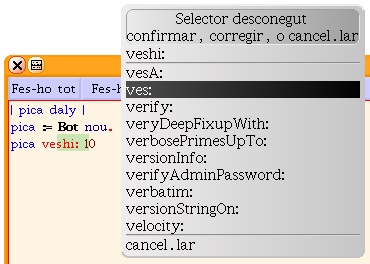
\includegraphics[height=50mm ,width=71mm ]{Imatges/figura2-5.png}
\end{center}
\caption{Hem escrit malament el missatge \textsf{\upshape ves:} escrivint \textsf{\upshape veshi:} per error. El missatge \textsf{\upshape veshi:} no existeix (a Squeak). Per tant Squeak suggereix possibles correccions.}
\label{fig0205}
\end{figure}

\subsection{Escriure malament el nom d'una variable}
\index{variables!errors relacionats amb|(}
\index{variable, nom de!escriure malament}
\index{errors en el programa!escriure malament el nom d'una variable}
Hi ha dues maneres d'escriure malament el nom d'una variable: en el cos de l'\emph{script} i quan es declara (entre barres verticals, com a $|$ \textsf{pica} $|$). La figura~\ref{fig0206} mostra els dos casos: A dalt hem declarat la variable \textsf{pica}, però hem escrit \textsf{pica1} a l'\emph{script}, enlloc de \textsf{pica}. Squeak s'ha adonat que intentàvem utilitzar una variable no declarada, de manera que l'ha acolorit de vermell i suggereix o bé que declarem la variable \textsf{pica1} com a nova variable, o bé que substituïm \textsf{pica1} per \textsf{pica}. Com que \textsf{pica} és el nom de variable que en realitat volem i \textsf{pica1} només era un error, triem l'opció \textsf{pica}, com es veu a la figura. A baix es mostra com hem escrit accidentalment un espai entre la \textsf{c} i la \textsf{a} en escriure \textsf{pica} mentre la declaràvem. Squeak no ha considerat que això sigui un error, simplement ha ``pensat'' que estàvem intentant declarar dues variables, \textsf{pic} i \textsf{a}. Aleshores, dins l'\emph{script} hem escrit \textsf{pica}, pensant que ja havíem declarat la variable. Squeak, però, ha detectat que \textsf{pica} és una variable no declarada de manera que l'ha acolorit de vermell i ens ha suggerit algunes opcions, incloent-hi declarar una nova variable amb nom \textsf{pica} o substituir el que hem escrit per la variable declarada \textsf{pic}. 

\begin{figure}[h]
\begin{center}
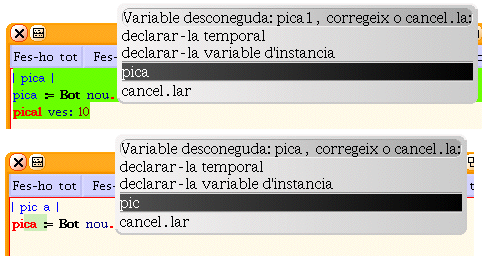
\includegraphics[height=50mm ,width=92mm ]{Imatges/figura2-6.png}
\end{center}
\caption{Dos exemples d'error. \emph{A dalt}: Hem escrit \textsf{\upshape pica1} enlloc del nom de la variable declarada \textsf{\upshape pica}. \emph{A baix}: Accidentalment hem escrit \textsf{\upshape pic a} quan provàvem de declarar la variable \textsf{\upshape pica}. Això té com a resultat la declaració de les variables \textsf{\upshape pic} i \textsf{\upshape a} i no de la variable \textsf{\upshape pica}.}
\label{fig0206}
\end{figure}

\subsection{Variables no utilitzades}
\index{errors en el programa!variables no utilitzades}
Pot pasar que accidentalment declareu massa variables. Per exemple, podríeu declarar les variables \textsf{pica} i \textsf{daly}, pensant que necessitareu dos robots, però no utilitzar mai \textsf{daly} a l'\emph{script}. Això no és realment un error, i el vostre programa podria executar-se correctament amb variables declarades i no utilitzades. Això és anàleg a comprar dues maletes, per si de cas, però utilitzar-ne només una. Simplement tenim equipatge extra que no fem servir. Tot i així, per si realment volíeu utiltzar \textsf{daly} i us n'heu oblidat, Squeak comprova si hi ha variables declarades i no utilitzades i, si en troba alguna, suggereix que potser voldríeu esborrar-la. Per exemple, a la figura~\ref{fig0207}, l'\emph{script} declara les variables \textsf{pica} i \textsf{daly} però només utilitza \textsf{pica}. Squeak s'adona d'això i pregunta si voldríeu esborrar la variable no utilitzada \textsf{daly}. \index{variables!errors relacionats amb|)}

\begin{figure}[h]
\begin{center}
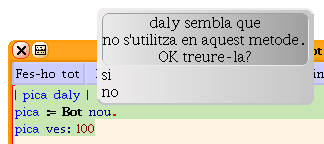
\includegraphics[height=40mm ,width=90mm ]{Imatges/figura2-7.png}
\end{center}
\caption{Totes les variables i els enviaments de missatges són correctes. La variable \textsf{\upshape daly}, però, s'ha declarat tot i no fer-la servir, de manera que Squeak ens ho fa notar i ens suggereix si voldríem esborrar-la. Les variables declarades i no utilitzades no són un error, però les coses com més senzilles millor, així que hauríem d'esborrar-la.}
\label{fig0207}
\end{figure}

\subsection{Majúscules o minúscules?}
\index{minúscules, lletres; errors relacionats amb}
\index{majúscules, lletres; errors relacionats amb}
\index{errors en el programa!majúscules versus minúscules}
Un altre error comú és oblidar que hi ha lletres que cal posar en majúscules. Els noms de les classes comencen amb un caràcter en majúscules, així que no ho oblideu quan vulgueu enviar un missatge a una fàbrica d'objectes. La figura~\ref{fig0208} ens mostra com hem escrit distretament \textsf{bot} enlloc de \textsf{Bot}. Squeak ha provat d'endevinar què és el que volíem dir, però no ha pogut i cap de les opcions que ofereix per arreglar el problema serveix. En aquest cas, cal que un mateix corregeixi l'error. En el context d'aquest llibre, les úniques classes de què us heu de preocupar són \textsf{Bot}, la fàbrica de robots, i \textsf{Color}, la fàbrica de colors.
\begin{figure}[h!]
\begin{center}
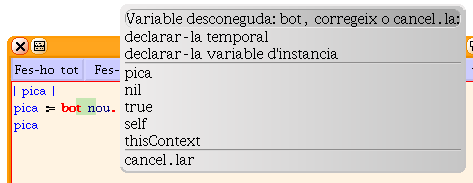
\includegraphics[height=45mm ,width=116mm ]{Imatges/figura2-8.png}
\end{center}
\caption{Hem oblidat la majúscula B al nom de la classe \textsf{\upshape Bot}, la fàbrica de robots. Squeak sap que alguna cosa no va bé, però no està segur de quina és. Haurem de corregir l'error nosaltres mateixos.}
\label{fig0208}
\end{figure}

\subsection{Oblidar un punt}
\index{. (punt)!oblidar un}
\index{punt (.)!oblidar un}
\index{missatges!oblidar punts entre}
\index{errors en el programa!oblidar un punt}
Finalment, un dels errors més comuns, un que fins i tot els programadors cometen, és oblidar un punt entre dos enviaments de missatge, o un punt i coma entre missatges en una cascada. Un punt indica que està a punt de començar un nou enviament de missatge, però sense el punt Squeak creu que el missatge actual continua, i que la variable que hauria de ser el receptor d'un nou missatge és només un altre selector de missatge. Com que no hi ha cap selector de missatge amb el nom de la variable, Squeak us diu que heu escrit un selector desconegut i us ofereix algunes correccions. Per exemple, a la figura~\ref{fig0209} no hi ha punt darrera l'expressió \textsf{pica := Bot nou}, i Squeak analitza (vull dir, intenta endevinar quina és l'estructura) el missatge  \textsf{pica := Bot nou pica ves: 120}, i d'acord amb les regles de la sintaxi (l'estructura) dels missatges, que aprendreu en el capítol~\ref{cap11}, \textsf{pica} hauria de ser un selector de missatge. Però aquest selector de missatge no existeix, de manera que Squeak es queixa i proposa algunes possibles substitucions. Com que vosaltres ja sabeu que  \textsf{pica} és la vostra variable declarada i no un selector de missatge, us adoneu que heu oblidat un punt, trieu ``cancel·lar'' i poseu el punt manualment.

\begin{figure}[h]
\begin{center}
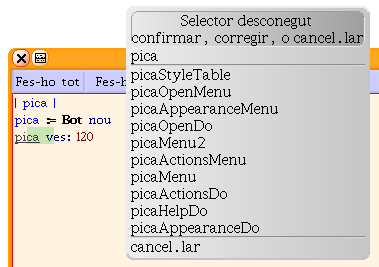
\includegraphics[height=55mm ,width=78mm ]{Imatges/figura2-9.png}
\end{center}
\caption{Les conseqüències d'oblidar un punt entre enviaments de missatges: Squeak creu que el receptor del missatge del segon enviament de missatge és un selector de missatge inexistent.}
\label{fig0209}
\end{figure}

\subsection{Paraules que canvien de color}
\index{color del text, canvis del}
\index{text, color; canvis del}
Squeak prova d'identificar els errors mentre esteu escrivint els vostres \emph{scripts}. Si detecta alguna cosa que no lliga amb el que espera, canvia el color del text i proporciona algunes indicacions visuals que suggereixen el que pot estar malament. La figura~\ref{fig0210} ens mostra algunes situacions típiques. Malauradament, si no veieu la figura en color haureu d'utilitzar la vostra imaginació!

\begin{figure}[h]
\begin{center}
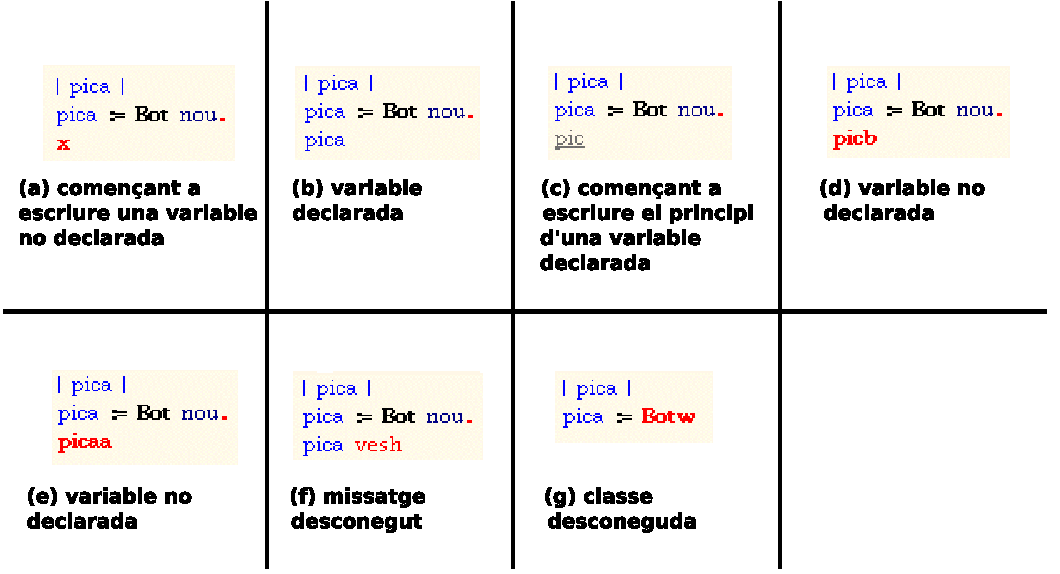
\includegraphics[scale=0.75]{Imatges/figura2-10}
\end{center}
\caption{Squeak utilitza colors per ajudar-vos a trobar errors i per saber si tot va bé.}
\label{fig0210}
\end{figure}

Aquí teniu una explicació més detallada de la figura:\index{errors en el programa|seealso{depurador; errors}} \index{errors en el programa!detectar amb el color del text|(}

\begin{itemize}
\item[\textbf{(a)}] Hem començat a escriure la primera lletra d'una variable desconeguda o no declarada. Com que no ha estat declarada cap variable començant amb la lletra x, Squeak l'acoloreix de vermell, fent-nos saber que alguna cosa està malament.
\item[\textbf{(b)}] Hem acabat d'escriure una variable que ha estat declarada. Squeak ens diu que hem escrit una variable declarada acolorint el nom de blau.
\item[\textbf{(c)}] Estem escrivint el nom d'una variable. Mentre el que anem escrivint es correspongui amb el començament del nom d'alguna variable declarada, Squeak el subratlla per fer-nos saber que fins ara tot és correcte.
\item[\textbf{(d)}] Tan aviat com escriguem un caràcter al nom de la variable de manera que la seqüència de caràcters ja no sigui el començament d'una variable declarada, Squeak acoloreix el text de vermell. Fixeu-vos en la diferència respecte del cas anterior. En el cas (c), podríem haver escrit el caràcter \textsf{a} i completar el nom de  la variable declarada \textsf{pica}, com en el cas (a). Hem escrit, però, el caràcter \textsf{b} i hem obtingut una seqüència de lletres (\textsf{picb}) que no és el començament del nom de cap variable declarada.
\item[\textbf{(e)}] Després d'escriure el nom d'una variable declarada (\textsf{pica}, com en el cas (b)), accidentalment hi hem afegit un caràcter més \textsf{a}, que dóna lloc a \textsf{picaa}, que no és el començament d'una variable declarada.
\item[\textbf{(f)}] Squeak intenta fer el mateix que fa amb els noms de les variables per als selectors de missatge. Aquí, hem escrit malament el missatge \textsf{ves:} i hem escrit \textsf{vesh} en el seu lloc. Squeak estava esperant un selector de missatge i tan aviat com hem escrit el caràcter \textsf{h}, s'ha adonat que no hi ha cap missatge que comenci per \textsf{vesh}, de manera que ha acolorit de vermell el que  estàvem escrivint.
\item[\textbf{(g)}] Squeak prova de fer el mateix amb les classes. Aquí hem escrit el caràcter \textsf{w} després de \textsf{Bot}, i Squeak, esperant un nom de classe ja que hem començat el nom amb \textsf{B} majúscula, acoloreix \textsf{Botw} de vermell ja que no hi ha cap classe al sistema el nom de la qual comenci així.
\end{itemize}
\index{errors en el programa!detectar amb el color del text|)}

\section{Resum}

\begin{itemize}
\item Per executar una expressió, premeu el botó \textbf{Fes-ho tot} de l'espai de treball.
\item Un \emph{script} és una seqüència d'expressions que fa alguna tasca.
\item Un missatge està compost d'un selector de missatge i possiblement un o més arguments. Alguns selectors de missatge no necessiten cap argument, com a l'enviament de missatge \textsf{pica tornarInvisible}.
\item Qualsevol selector de missatge que acaba amb dos punts requereix informació addicional (un o més arguments), com una longitud o un angle. Per exemple, el selector de missatge \textsf{giraEsquerra:} necessita un argument el valor del qual és un nombre que representa l'angle que el robot hauria de girar en sentit contrari a les agulles del rellotge.
\item Per obtenir un objecte nou, usualment cal enviar el missatge \textsf{nou} a una classe. Per exemple, \textsf{Bot nou} crea un robot nou. Pot ser que altres classes entenguin altres missatges per crear objectes nous. Per exemple, \textsf{Color groc} demana a la classe \textsf{Color} que creï un color groc nou.
\item Una classe és una fàbrica per produir objectes. Els noms de les classes sempre s'han de fer començar amb una lletra majúscula. Per exemple, \textsf{Bot} és la fàbrica per crear nous robots, i \textsf{Color} és la fàbrica de colors. EL missatge \textsf{Bot nou color: Color groc} demana a la classe \textsf{Bot}  que creï un robot nou, i després demanem a la fàbrica de colors que fabriqui un nou objecte color groc. Finalment, el missatge \textsf{color:} s'envia al nou robot amb el nou objecte color groc com a argument, resultant en un robot nou de color groc.
\item Els enviaments de missatges han de ser separats amb un punt. No cal posar un punt al final, després del darrer enviament de missatge. Aquí teniu un exemple de quatre enviaments de missatge separats per tres punts:

\noindent
\textsf{\upshape
\\
pica := Bot nou.\\
pica ves: 100.\\
pica giraEsquerra: 90.\\
pica ves: 100\\
}
\item Per enviar múltiples missatges al mateix objecte podeu utilitzar un punt i coma per separar els missatges, com a \textsf{unBot} \emph{missatge1 ; missatge2}. Per exemple, \textsf{pica ves: 100 ; giraEsquerra: 90 ; ves: 200 ; giraEsquerra: 200} envia una seqüència de quatre missatges (1) \textsf{ves: 100}, (2) \textsf{giraEsquerra: 90}, (3) \textsf{ves: 200}, (4) \textsf{giraEsquerra: 200} al robot anomenat \textsf{pica}.
\end{itemize}

\index{ifTrue:ifFalse:, mètode|see{siCert:siFals:}}
\index{ifFalse:, mètode|see{siFals:}}
\index{whileTrue: bucle|see{mentreCert: bucle}}   
\index{whileFalse: bucle|see{mentreFals: bucle}}   

\chapter{Homes i robots}
\label{cap3}

\begin{center}
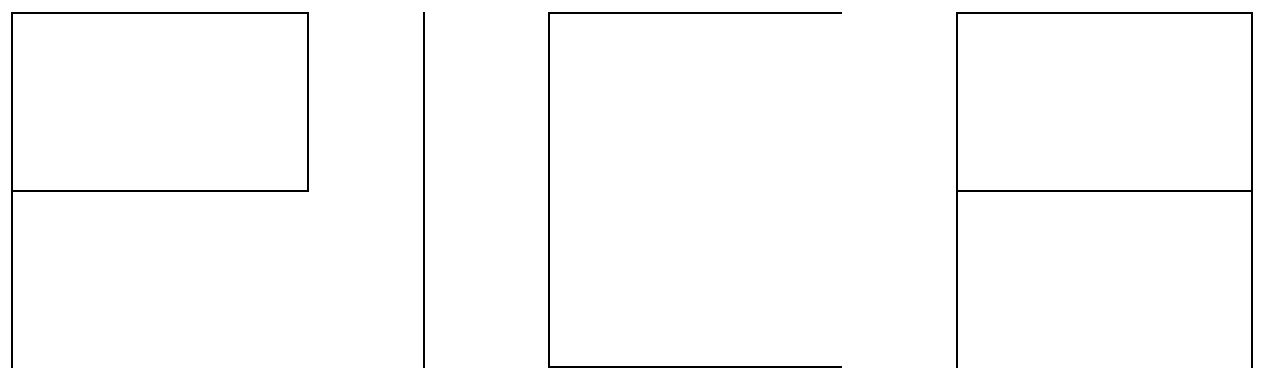
\includegraphics[height=40mm ,width=\textwidth ]{Imatges/figura3-0}
\end{center}

En aquest capítol\footnote{\emph{Nota del Traductor:} El títol del capítol en anglès és \emph{Of Robots and Men} recordant el títol de la novel·la de John Steinbeck \emph{Of Mice and Men}. D'acord amb la traducció al català de la novel·la publicada per l'editorial La Galera, el títol traduït de la novel·la és ``Homes i Ratolins''. Per tant, he traduït el títol del capítol per mantenir la coherència amb la traducció catalana de l'obra d'Steinbeck.} descrivim la creació de robots i els diferents tipus de moviments que els robots coneixen i són capaços de realitzar.  Perque pugueu practicar el que heu après en capítols anteriors, us proposem alguns experiments senzills. També us ensenyarem com els robots poden canviar de direcció seguint els punts cardinals. 

\section{Crear robots}
\index{robots!crear}
\index{classes|seealso{fàbriques de robots}}
\index{classes!crear objectes}
\index{classes!com a fàbriques}
Al capítol anterior heu creat \emph{un} robot, no \emph{el} robot. Volem dir que els robots no són únics, i que podeu crear tants robots com vulgueu. L'\emph{Script}~\ref{scr3-1} crea dos robots: \textsf{pica} i  \textsf{daly}. \index{daly, crear robot} \index{pica, robot!crear}

\begin{script}  El naixement de dos robots.
\noindent
\textsf{\upshape
\\
\\$|$ pica daly $|$\\
pica := Bot nou.\\
daly := Bot nou.\\
pica color: Color groc.\\
daly salta: 100.\\
}
\label{scr3-1}
\end{script}

La segona línia crea un robot anomenat \textsf{pica}, com a l'\emph{script}~\ref{scr2-1}. La tercera línia crea un robot nou a què ens referirem utilitzant la variable \textsf{daly} (igual que vam fer amb la variable \textsf{pica}, el nom de la qual és un homenatge a Pablo Picasso, el nom de la variable \textsf{daly} és un homenatge a Salvador Dalí). Tots dos robots són creats al mateix lloc de la pantalla. A la línia quatre, li diem a \textsf{pica} que canviï el seu color a groc de manera que puguem distingir els dos robots.

Tal i com ja hem dit abans, Smalltalk és un llenguatge orientat a objectes. Això no només significa que podem crear objectes i interactuar amb ells, sinó que a més els objectes poden crear altres objectes i comunicar-se amb ells. És més, a Smalltalk hi ha objectes especials, anomenats \emph{classes}, que s'utilitzen per crear objectes. En general, enviant el missatge \textsf{new} a una classe creem un objecte tal i com és descrit a la classe. Enviar el missatge \textsf{nou} a la classe \textsf{Bot} crea un robot.\index{fàbriques!classes com a}

Per entendre què són les classes, imagineu una classe com una mena de fàbrica. Una fàbrica per crear capses pot fabricar un gran nombre de capses sense cap ús en especial, totes de la mateixa forma, mida i color. Després de fabricades, algunes capses poden acabar contenint galetes i d'altres es poden trencar. Quan una capsa es trenca, les altres capses no es veuen afectades. El mateix passa amb els objectes creats dins d'Squeak. En el nostre cas, \textsf{daly} no ha canviat de color, tot i que \textsf{pica} sí que ho ha fet, mentre que \textsf{pica} no s'ha mogut i \textsf{daly} sí. Podeu pensar en una classe com en una fàbrica capaç de produir un nombre il·limitat d'objectes d'un mateix tipus. Un cop fabricats, cada objecte existeix independentment dels altres i el podem modificar tan com vulguem.\index{objectes!crear per classes}

A Smalltalk, els noms de les classes sempre comencen amb una lletra majúscula. Aquesta és la raó per la qual el nom de la classe robot és \textsf{Bot}, amb ``B'' majúscula. Fixeu-vos que a la instrucció \textsf{Color groc}, la paraula \textsf{Color} s'ha escrit amb una ``C'' majúscula. Això és per que \textsf{Color} és una classe, i el que fabrica són objectes color. Especificant el nom del color, obtenim un objecte color del color que volem (l'expressió \textsf{Color groc} és una manera abreujada de crear un objecte color groc. Primer es crea un objecte color enviant el missatge \textsf{new} a la classe\textsf{Color}, i després alguns missatges més defineixen l'objecte color com a groc). \index{Smalltalk!llenguatge de programació}

\newpage

\noindent
\rule{\textwidth}{2pt}
\noindent
\textbf{Important!} Una classe és una fàbrica que manufactura objectes. En general, enviant el missatge \textsf{new} a una classe creem un objecte d'aquella classe. Els noms de les classes sempre comencen amb una lletra majúscula. Aquí, \textsf{Bot} és el nom de la fàbrica per crear nous robots, i \textsf{Color} és la fàbrica de colors.

\noindent
Així, l'enviament de missatge \textsf{Bot nou color: Color blau} envia un missatge a la classe \textsf{Bot} per crear un robot nou i després envia un missatge al nou robot perquè s'acoloreixi ell mateix de blau. \index{colors!canviar-los en els robots} \index{robots!canviar els colors}

\noindent
\rule{\textwidth}{2pt}

\section{Dibuixar segments de línia}
\index{ves missatge!avançar píxels}
\index{segments de línia, dibuixar}
Demanar a un robot que dibuixi una línia és força senzill, tal com heu vist al capítol anterior. El missatge \textsf{ves: 100} li diu al robot que es mogui endavant 100 píxels, i el robot deixa una marca mentre es mou. Quan dibuixem, però, cal que de tant en tant aixequem el llapis del paper, fins i tot si som uns escriptors experts en cal·ligrafia xinesa o japonesa. Per això, un robot sap saltar; és a dir, el robot sap moure's sense deixar cap traça. Els robots entenen el missatge \textsf{salta:} l'argument del qual és el mateix que per al missatge \textsf{ves:}, una distància donada en píxels. L'\emph{Script}~\ref{scr3-2} dibuixa dos segments. Per què quedi clar el que dibuixen els robots, aquests s'han fet desaparèixer de la il·lustració tot enviant-los el missatge \textsf{tornarInvisible}.\index{salta: missatges!efecte de}

\begin{script}  Creem pica i després dibuixa dues línies.
\newline
\newline
\noindent
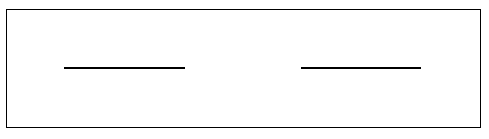
\includegraphics[height=10mm ,width=40mm]{Imatges/figuraS3-2.png}
\noindent
\textsf{\upshape
\\
\\$|$ pica $|$\\
pica := Bot nou.\\
pica ves: 30.\\
pica salta: 30.\\
pica ves: 30.\\
}
\label{scr3-2}
\end{script}

\index{Experiments|seealso{\emph{Scripts}}}
\begin{center}
\colorbox{black}{\makebox[\textwidth]{  \color{white} {\large {\bfseries Experiment 3-1 (crear i moure un robot)}} }}
\end{center}
\index{crear i moure un robot, Experiment}
\index{Experiments!crear i moure un robot}
\index{Morse, codi; dibuixar missatge SOS en}
\index{SOS missatge en codi morse, dibuixar}
{\small
\noindent
Experimenteu canviant els valors de l'\emph{script} anterior.}\\
\noindent
\rule{\textwidth}{3pt}

\newpage

\begin{center}
\colorbox{black}{\makebox[\textwidth]{  \color{white} {\large {\bfseries Experiment 3-2 (SOS)}} }}
\end{center}
\index{SOS, Experiment}
\index{Experiments!SOS}
{\small
\noindent
Escriviu un \emph{script} que dibuixi el missatge ``SOS'' en codi Morse (en codi Morse, una ``S'' es representa amb tres línies curtes i una ``O'' amb tres línies llargues, com mostrem a la figura)}
\begin{center}
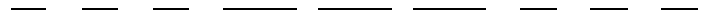
\includegraphics[height=3mm ,width=90mm]{Imatges/figuraE3-2.png}
\end{center}
\noindent
\rule{\textwidth}{3pt}
\index{direccions absolutes!significat de|(}
\section{Canviar de direcció}
\index{canviar de direcció|(}
\index{direcció!canviar de|(}
Un robot es pot orientar en les vuit direccions principals d'una brúixola, com es pot veure a la figura~\ref{fig0301}. Les direccions són com les d'un mapa normal i corrent: est és a la dreta, oest és a l'esquerra, nord és amunt i sud és avall. Aquestes direccions són \emph{absolutes}, la qual cosa significa que no importa en quina direcció estigui apuntant el robot, si li diem que apunti a l'\textsf{est}, el robot apuntarà a la dreta de la pantalla, no a la seva dreta. Per apuntar un robot  en una direcció absoluta, només cal enviar-li un missatge amb el nom de la direcció. Així, si volem que \textsf{pica} apunti al sud, simplement escrivim \textsf{pica sud}. \index{brúixola, apuntar els robots en les direccions principals de la} \index{robots!apuntar en les direccions principals de la}

\begin{figure}[h]
\begin{center}
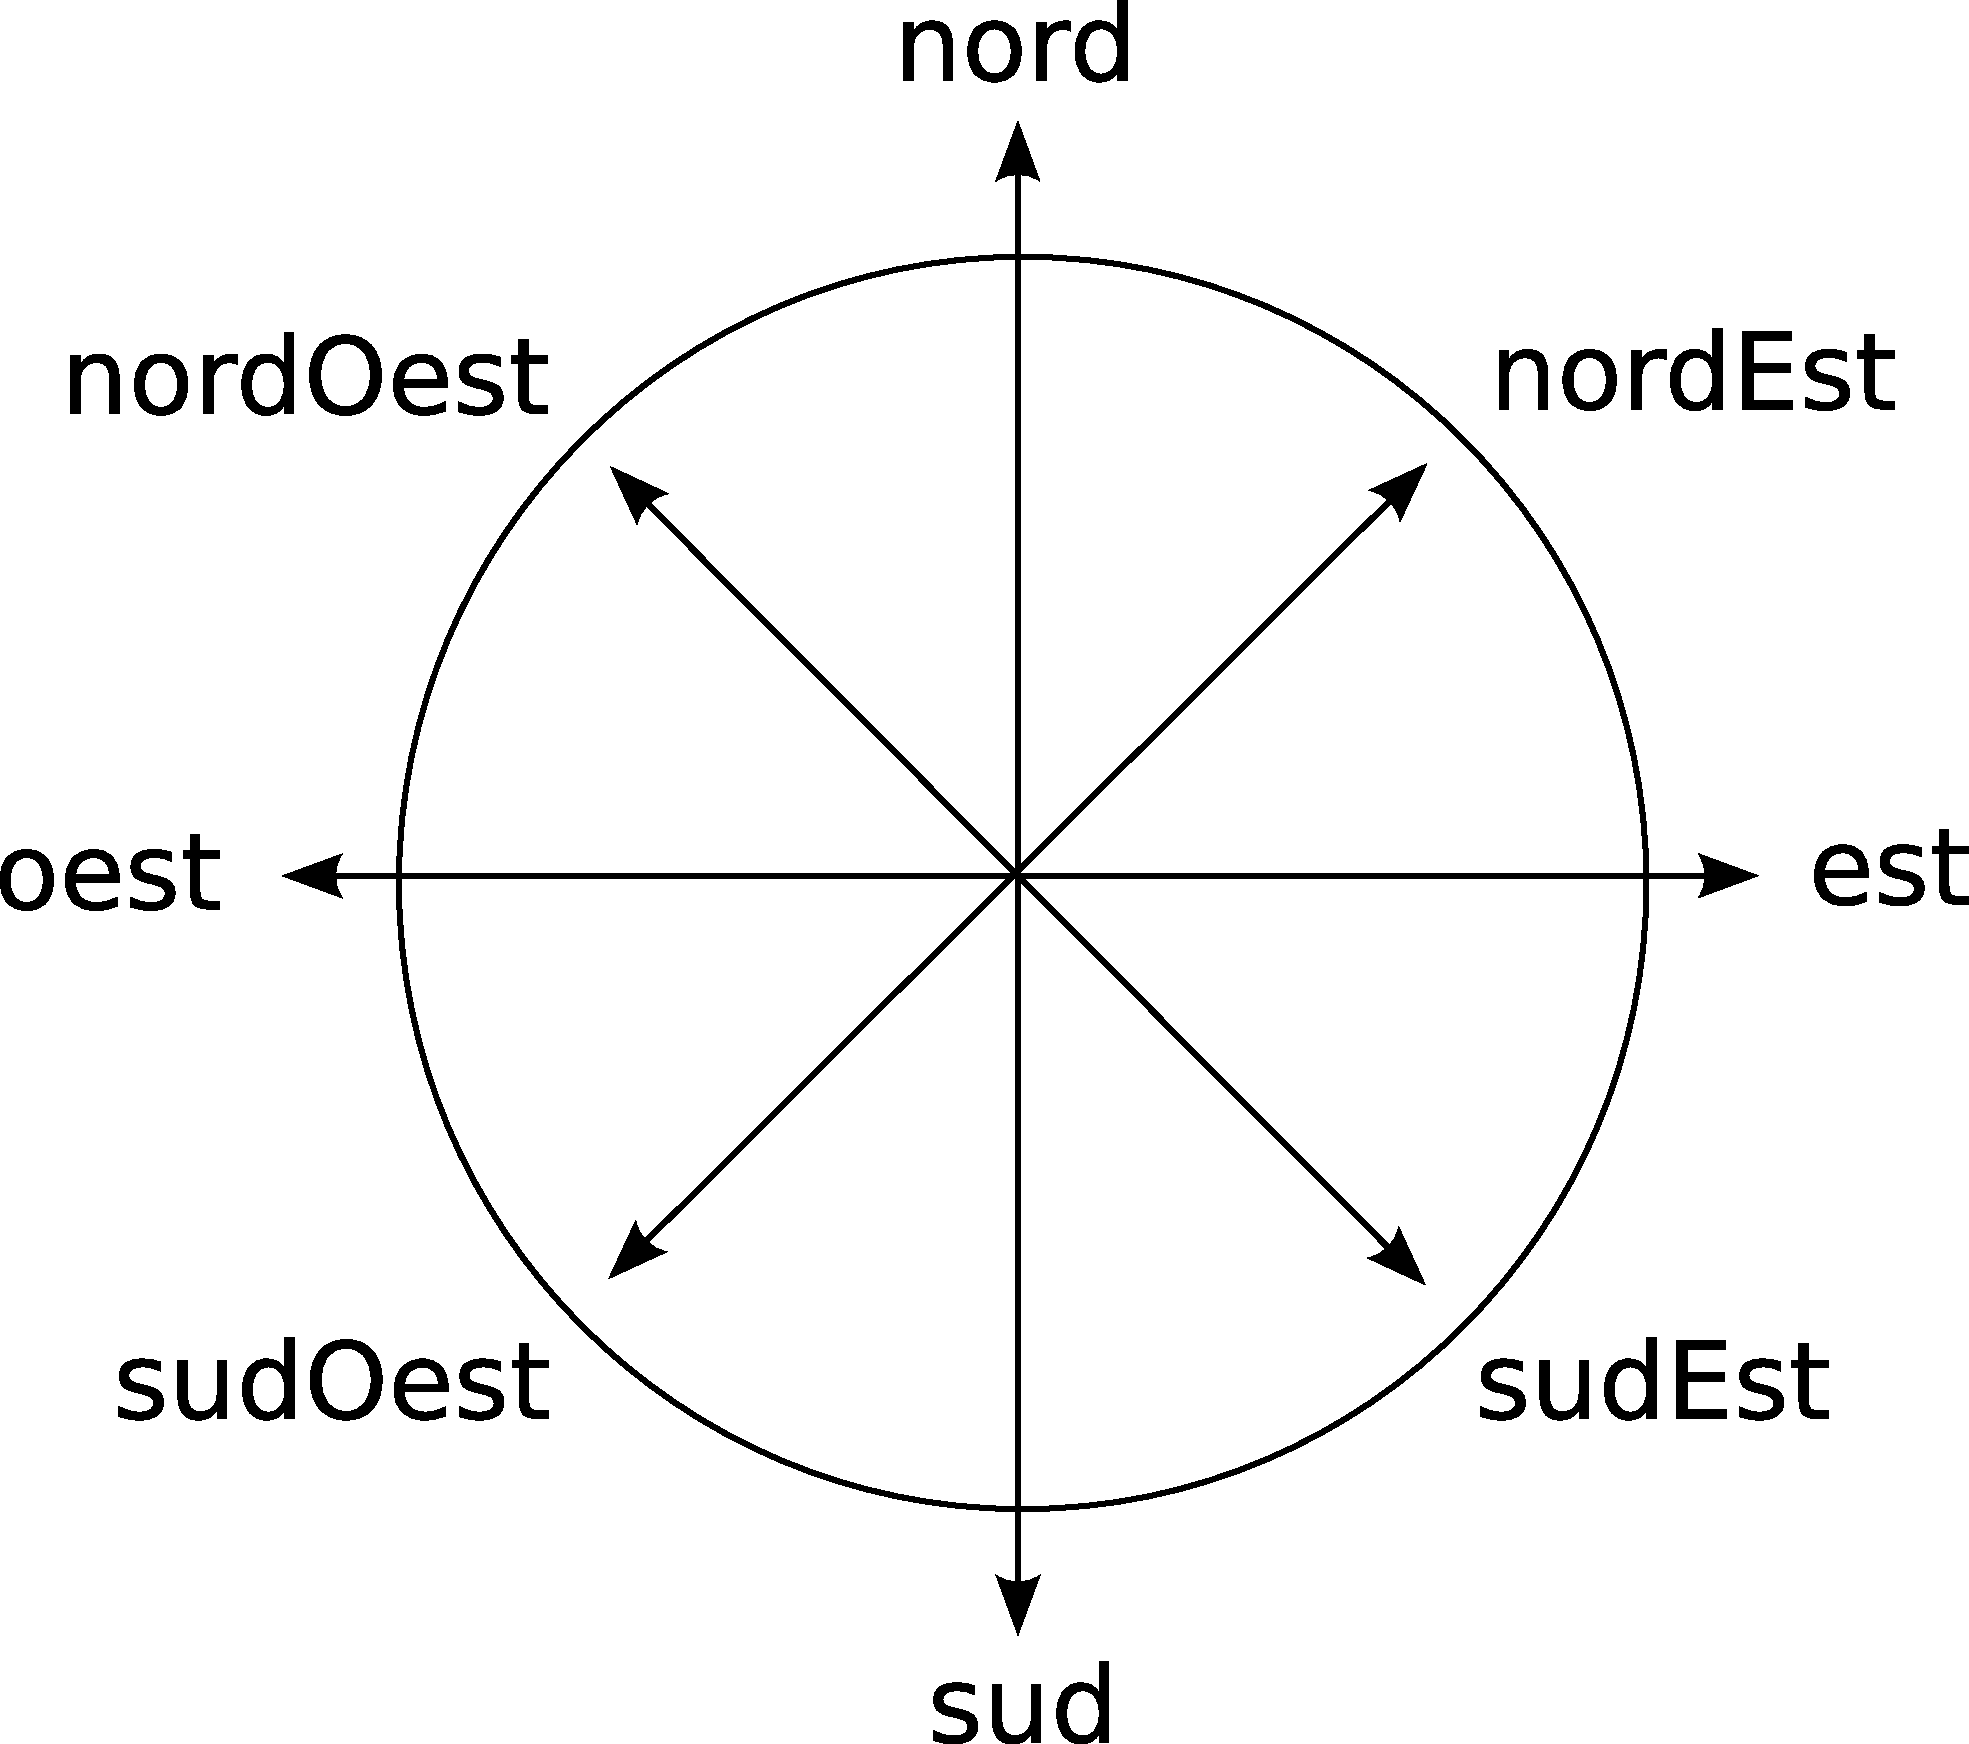
\includegraphics[scale=0.25]{Imatges/figura3-1}
\end{center}
\caption{Les direccions absolutes d'una brúixola a què un robot pot apuntar.}
\label{fig0301}
\end{figure}

Els robots entenen els següents missatges de direcció respecte als punts cardinals: \textsf{est}, \textsf{nord}, \textsf{nordEst}, \textsf{nordOest}, \textsf{sud}, \textsf{sudEst}, \textsf{sudOest} i  \textsf{oest}. Al proper capítol, us ensenyarem com fer que un robot giri un angle qualsevol de manera relativa a la seva posició actual. \index{est missatge, exemple de} \index{oest missatge, exemple de} \index{nord missatge, exemple de} \index{sud missatge, exemple de} \index{sudEst missatge, exemple de} \index{sudOest missatge, exemple de} \index{nordEst missatge, exemple de} \index{nordOest missatge, exemple de} 

L'\emph{Script}~\ref{scr3-3} il·lustra les quatre direccions cardinals amb quatre robots diferents; aquí Picasso i Dali són acompanyats per Paul Klee i Alfred Sisley. Excepte per \textsf{pica}, que es manté en la direcció \textsf{est}, on apunten per defecte els robots, hem orientat a cada robot en una direcció diferent abans de dir-li que es mogui.

\begin{script}  Un grup de robots en moviment.
\noindent
\textsf{\upshape
\\
\\$|$ pica daly klee sisl $|$\\
pica := Bot nou.\\
pica color: Color verd.\\
pica ves: 100.\\
daly := Bot nou.\\
daly nord.\\
daly color: Color groc.\\
daly ves: 100.\\
klee := Bot nou.\\
klee oest.\\
klee color: Color vermell.\\
klee ves: 100.\\
sisl := Bot nou.\\
sisl sud.\\
sisl ves: 100.
}
\label{scr3-3}
\end{script}

\vspace*{2mm}
\index{direccions absolutes!significat de|)}

\noindent
Podeu utilitzar aquests mètodes d'orientació per fer dibuixos molt més complicats.

\begin{center}
\colorbox{black}{\makebox[\textwidth]{  \color{white} {\large {\bfseries Experiment 3-3 (quadrat)} }}}
\end{center}
\index{quadrat @quadrat, Experiment}
\index{Experiments!quadrat @quadrat}
{\small
\noindent
Com a primer exercici, dibuixeu un quadrat de costat 50 píxels. Després dibuixeu-ne un altre de costat 250 píxels.}\\
\noindent
\rule{\textwidth}{3pt}

\newpage

\begin{center}
\colorbox{black}{\makebox[\textwidth]{  \color{white} {\large {\bfseries Experiment 3-4 (escala)} }}}
\end{center}
\index{escala, Experiment}
\index{Experiments!escala}
{\small
\noindent
No només podeu dibuixar quadrats. Podeu crear un ampli ventall de figures geomètriques. Per exemple, aquí teniu el dibuix d'una petita escala. Escriviu un \emph{script} per reproduir aquest dibuix.}
\begin{center}
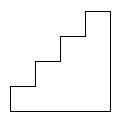
\includegraphics[height=25mm ,width=25mm]{Imatges/figuraE3-4.png}
\end{center}
\noindent
\rule{\textwidth}{3pt}

\begin{center}
\colorbox{black}{\makebox[\textwidth]{  \color{white} {\large {\bfseries Experiment 3-5 (la piràmide esglaonada de Saqqara)}} }}
\end{center}
\index{piràmide esglaonada@la piràmide esglaonada de Saqqara, Experiment}
\index{Experiments!piràmide esglaonada@la piràmide esglaonada de Saqqara}
{\small
\noindent
Ara ja podeu desplegar el vostre enginy arquitectònic i dibuixar una vista esquemàtica de la piràmide esglaonada de Saqqara, construïda cap al 2900 a.c. per l'arquitecte Imhotep. Feu un \emph{script} que dibuixi una vista lateral de la piràmide (veieu la figura). La piràmide té quatre esglaons, i la part superior és el doble de llarga que cada esglaó.}
\begin{center}
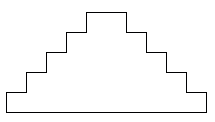
\includegraphics[height=20mm ,width=35mm]{Imatges/figuraE3-5.png}
\end{center}
\vspace*{-1mm}
\noindent
\rule{\textwidth}{3pt}

\begin{center}
\colorbox{black}{\makebox[\textwidth]{  \color{white} {\large {\bfseries Experiment 3-6 (art abstracte)} }}}
\end{center}
\index{art abstracte, Experiment}
\index{Experiments!art abstracte}
{\small
\noindent
Escriviu un \emph{script} per reproduir el dibuix d'aquesta figura.}
\begin{center}
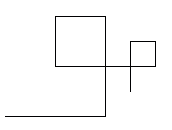
\includegraphics[height=30mm ,width=40mm]{Imatges/figuraE3-6.png}
\end{center}
\noindent
\rule{\textwidth}{3pt}
\index{canviar de direcció|)}

\section{L'ABC del dibuix}
\index{A!dibuixar|(}
\index{lletra A!dibuixar|(}
\index{direcció!canviar de|)}
\index{dibuixar!ABC del}
Fins i tot sense tenir encara gaire control sobre la direcció en què el vostre robot dibuixa segments de línia, podeu començar a programar a \textsf{pica} per dibuixar lletres. L'\emph{Script}~\ref{scr3-4} dibuixa una ``A'' més aviat primitiva.

\begin{script}  Dibuixem la lletra A.
\newline
\noindent
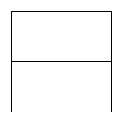
\includegraphics[height=30mm ,width=31mm]{Imatges/figuraS3-4.png}
\noindent
\textsf{\upshape
\\
\\$|$ pica $|$\\
pica := Bot nou.\\
pica nord.\\
pica ves: 100.\\
pica est.\\
pica ves: 100.\\
pica sud.\\
pica ves: 100.\\
pica nord.\\
pica ves: 50.\\
pica oest.\\
pica ves: 100.\\
}
\label{scr3-4}
\end{script}

Dibuixar una lletra ``C'' no és més difícil. Podeu fins i tot escriure la paraula ``pica''.

\begin{center}
\colorbox{black}{\makebox[\textwidth]{  \color{white} {\large {\bfseries Experiment 3-7 (PICA)} }}}
\end{center}
\index{PICA, Experiment}
\index{Experiments!PICA}
\index{salta: mètode, utilitzar a l'experiment PICA}
{\small
\noindent
Dibuixeu el nom ``pica'' tal com es mostra al principi d'aquest capítol. Per separar les lletres individuals hauríeu d'utilitzar el missatge \textsf{salta:}}\\
\noindent
\rule{\textwidth}{3pt}

\newpage

\noindent
\rule{\textwidth}{2pt}
\noindent
\textbf{Observació} Es podria argumentar que l'\emph{script}~\ref{scr3-4} es pot millorar. Per exemple, la meitat inferior de la línia vertical de la dreta de la ``A'' s'ha dibuixat dues vegades, ja que el robot retorna sobre aquest segment --un cop anant cap al nord, un altre cop anant cap al sud-- per posar-se en posició de dibuixar la línia horitzontal. Decidir quina és la millor manera de resoldre un problema de programació pot ser difícil. Hi ha molts aspectes del problema a considerar, tals com la rapidesa, la complexitat o la llegibilitat del codi, i aquestes qüestions tindran diferentes respostes depenent de quin llenguatge de programació i quins mètodes s'hagin fet servir. Tot i així, podem considerar una primera aproximació triant la solució més senzilla. Aleshores, si estem insatisfets perquè el programa és massa lent o perquè no té les peculiaritats que desitjaríem, sempre podem modificar-lo per fer-lo més ràpid o afegir-li més ampliacions.\\
\noindent
\rule{\textwidth}{2pt}
\index{A!dibuixar|)}
\index{lletra A!dibuixar|)}
\section{Controlar la visibilitat del robot}
\index{visibilitat i invisibilitat, aplicar als robots}
\index{visibilitat del robot, controlar}
\index{robots!tornar invisible}
\index{robots!moure}
Podeu controlar si un robot es mostra a la pantalla utilitzant els missatges \textsf{tornarInvisible} i \textsf{tornarVisible}. El missatge \textsf{tornarInvisible} amaga al receptor del missatge. Un robot ocult actua exactament com un de visible, però no ens ensenya on és. Aneu amb compte de no utilitzar el mètode \textsf{hide} (vol dir amagar), que està definit a Squeak pel seu ús particular i pot fer malbé l'entorn dels robots si s'utilitza inadequadament. El missatge \textsf{tornarVisible} fa que el robot receptor del missatge sigui visible. Un robot nou és visible per defecte.\index{invisibilitat i visibilitat, aplicar als robots} \index{variables!declarar per \emph{scripts}}

\newpage

\section{Resum}
\index{direcció!canviar de} \index{scripts@\emph{scripts}!declarar variables pels}
La taula següent resumeix les expressions i missatges apareguts en aquest capítol.
\index{colors!canviar-los en els robots} \index{robots!canviar colors} \index{robots!crear}

\vspace*{5mm}

\noindent
\setlength{\extrarowheight}{1mm}
{\small \begin{tabular}{p{50mm}p{50mm}p{40mm}}
\hline
\textbf{Expressions / Missatges}
&
\textbf{Descripció}
&
\textbf{Exemple}
\\
\hline
\textsf{Bot nou}
&
Crea un robot.
&
\textsf{pica := Bot nou}
\\
\textsf{$|$ x y $|$}
&
Declara variables per utilitzar en un \emph{script}
&
\textsf{$|$ pica $|$}
\\
\textsf{salta: {\itshape unEnter}}
&
Diu al robot que s'ha de moure endavant un determinat nombre de píxels sense deixar cap traça
&
\textsf{pica salta: 10}
\\
\textsf{ves: {\itshape unEnter}}
&
Diu al robot que s'ha de moure endavant un determinat nombre de píxels deixant una marca
&
\textsf{pica ves: 10}
\\
\textsf{tornarInvisible}
&
Diu al robot que s'ha de tornar invisible
&
\textsf{pica tornarInvisible}
\\
\textsf{tornarVisible}
&
Diu al robot que s'ha de tornar visible
&
\textsf{pica tornarVisible}
\\
\textsf{est, nordEst, nord, nordOest, oest, sudOest, sud, sudEst}
&
Diu al robot que ha d'apuntar en una determinada direcció
&
\textsf{pica nord}
\\
\textsf{Color {\itshape nomDeColor}}
&
Crea el color \textit{nomDeColor}
&
\textsf{Color blau}
\\
\textsf{color: {\itshape unColor}}
&
Demana al robot que canviï de color
&
\textsf{pica color: Color vermell}
\\
\hline
\end{tabular}}


\chapter{Direccions i angles}
\label{cap4}

\begin{center}
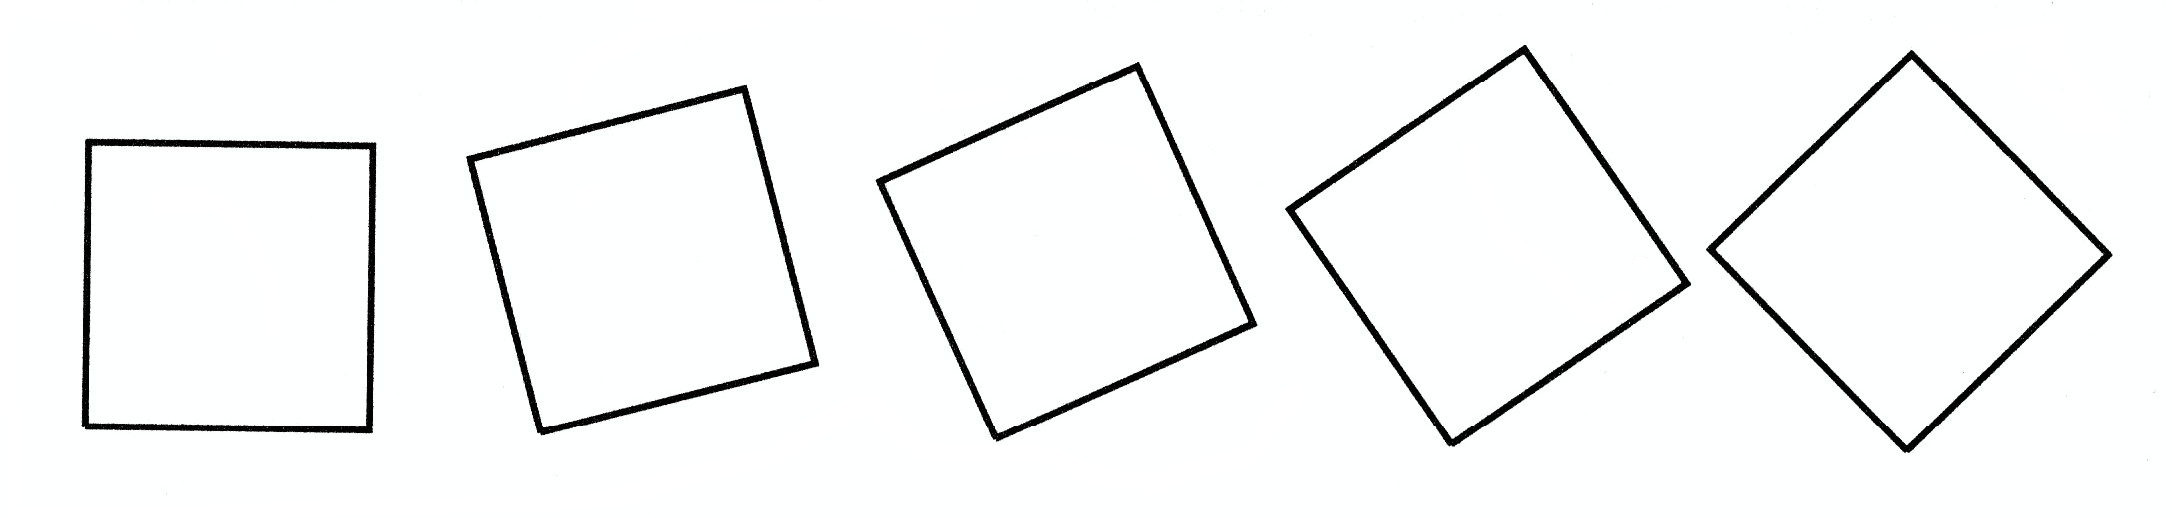
\includegraphics[height=35mm ,width=\textwidth ]{Imatges/figura4-0.jpg}
\end{center}

Ara ja hauríeu d'estar cansats de dibuixar figures només seguint direccions \emph{fixades}. En aquest capítol aprendreu com canviar la direcció a què apunta un robot, permetent al robot apuntar a \emph{qualsevol} direcció, girar qualsevol angle relatiu a la seva posició actual, i, per tant, dibuixar línies en qualsevol direcció. Si enteneu bé què és un angle i com mesurar angles en graus, podeu saltar la secció ``L'Enfocament Adequat'' i seguir amb els exemples i experiments de la secció ``Dibuixos Senzills''.

Començarem presentant els missatges elementals que els robots entenen per canviar de direcció. Amagarem els robots de les il·lustracions utilitzant el missatge \textsf{tornarInvisible} de manera que els dibuixos es vegin més clars.\index{tornarInvisible i tornarVisible mètodes, efectes de}

\section{Dreta o esquerra?}
\index{giraDreta: missatge, efecte de|(}
\index{giraEsquerra: missatge, efecte de|(}
Al capítol anterior vau aprendre que podíem fer que un robot apuntés a diferents direccions amb els missatges \textsf{est}, \textsf{nord}, \textsf{nordEst}, \textsf{nordOest}, \textsf{sud}, \textsf{sudEst}, \textsf{sudOest} i \textsf{oest}. Amb aquests missatges, però, no podeu canviar la direcció del vostre robot un angle qualsevol, com per exemple 15 graus. A més, tampoc podeu fer girar un robot, diguem, un quart de circumferència respecte de la seva posició actual.

Per girar un robot un determinat angle hem d'utiltzar els mètodes \textsf{giraEsquerra:} i \textsf{giraDreta:}, que ordenen al robot girar a la dreta o a l'esquerra. Tal com indiquen els dos punts al final del nom dels mètodes, tots dos mètodes esperen un argument. Aquest argument és l'angle que el robot hauria de girar relatiu a la seva posició actual. És a dir, l'argument és la diferència entre la direcció del robot abans que el missatge fos enviat i la seva direcció després que el missatge sigui enviat. L'angle es dóna en graus. Per exemple, l'expressió \textsf{pica giraEsquerra: 15} demana a \textsf{pica} que giri a l'esquerra 15 graus partint de la seva posició actual, i \textsf{pica giraDreta: 30} fa girar \textsf{pica} a la dreta trenta graus partint de la seva posició actual. La figura~\ref{fig0401} il·lustra l'efecte dels missatges \textsf{giraEsquerra:} i \textsf{giraDreta:}, primer, quan un robot apunta a l'\textsf{est} i segon, quan un robot apunta a alguna altra direcció. \index{robots!girar un angle determinat}

A mesura que aneu practicant fent girar els robots diversos angles, tingueu en compte que quan es crea un robot nou, sempre apunta cap a l'est, és a dir, a la dreta de la pantalla.

\begin{figure}[h!]
\begin{center}
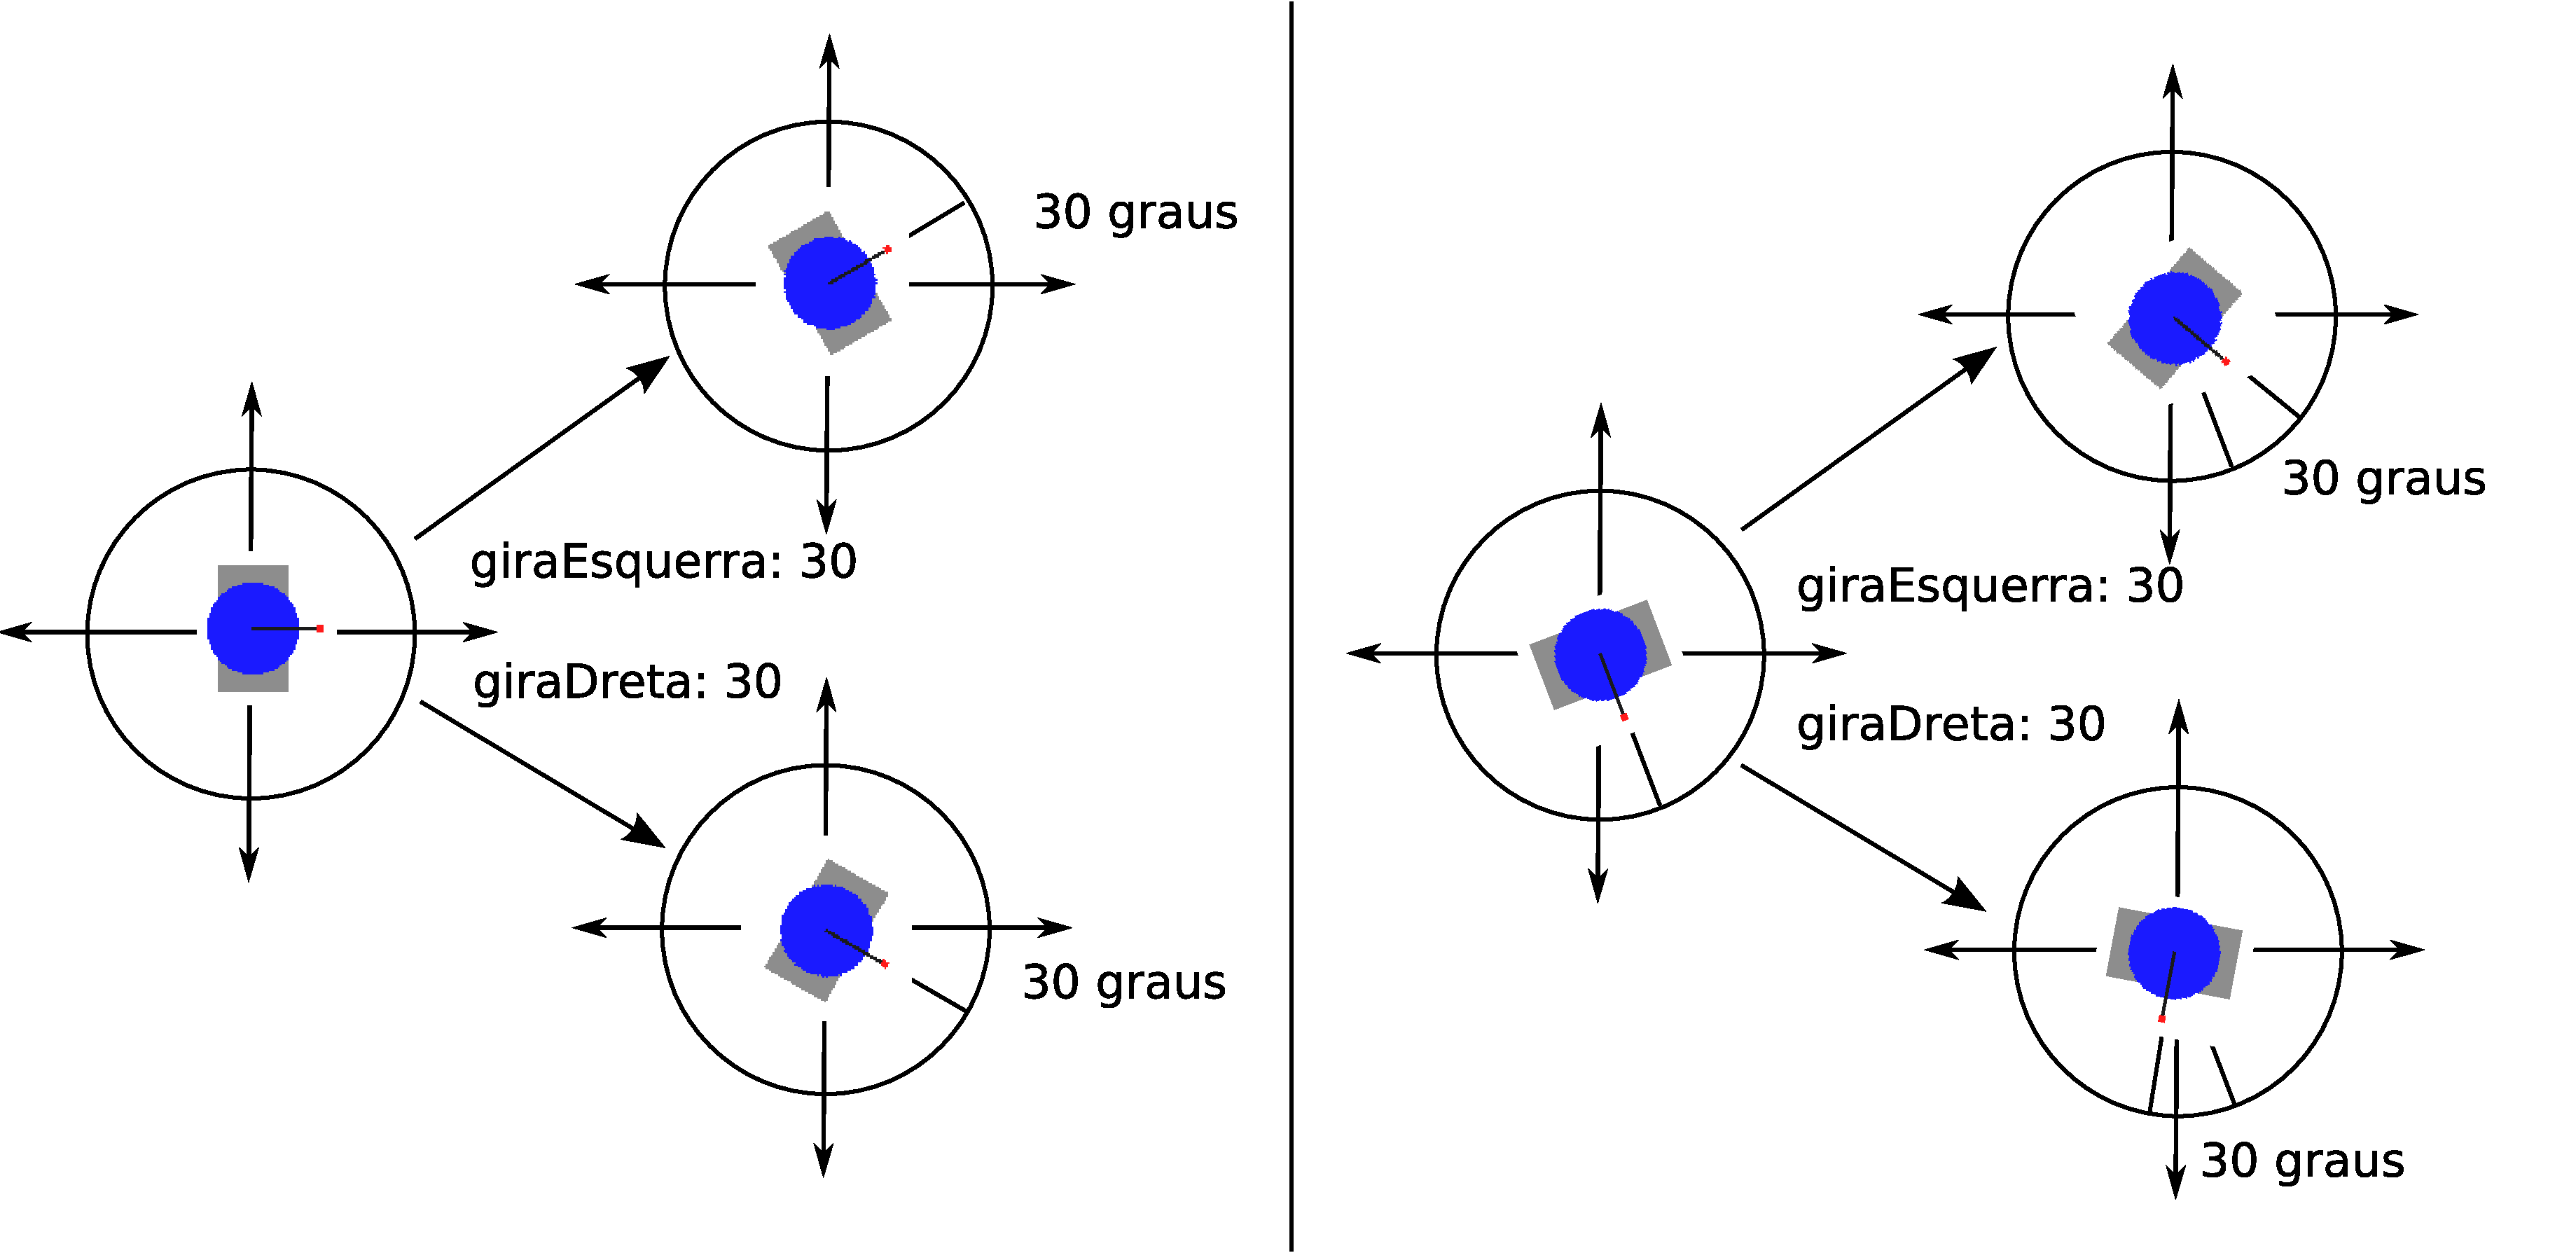
\includegraphics[scale=0.25]{Imatges/figura4-1}
\end{center}
\caption{\emph{Esquerra:} Un robot apuntant a l'est gira 30 graus a l'esquerra o a la dreta.
\emph{Dreta:} Un robot apuntant a una altra direcció gira 30 graus a l'esquerra o a la dreta.}
\label{fig0401}
\end{figure}

\newpage

\begin{center}
\colorbox{black}{\makebox[\textwidth]{  \color{white} {\large {\bfseries Experiment 4-1 (\emph{scripts} misteriosos)} }}}
\end{center}
\index{scripts misteriosos@\emph{scripts} misteriosos, Experiment}
\index{Experiments!scripts misteriosos@\emph{scripts} misteriosos}
{\small
\noindent
Els \emph{Scripts}~\ref{scr4-1} i~\ref{scr4-2} són problemes en els quals heu d'endevinar què farà el robot creat a cada \emph{script}. Després que estudieu aquests dos \emph{scripts}, experimenteu amb ells canviant-los els valors dels angles, per exemple, per determinar quin angle fa que el robot giri un quart de circumferència, mitja circumferència o una circumferència sencera. Si us cal revisar la noció d'angle, llegiu la secció ``L'Enfocament Adequat'' abans de continuar.}\\
\noindent
\rule{\textwidth}{3pt}

\begin{script}  Què fa pica? (Problema 1)
\noindent
\textsf{\upshape
\\
\\$|$ pica $|$\\
pica := Bot nou.\\
pica ves: 100.\\
pica giraEsquerra: 45.\\
pica ves: 50.\\
pica giraEsquerra: 45.\\
pica ves: 100.\\
}
\label{scr4-1}
\end{script}

\begin{script}  Què fa pica? (Problema 2)
\noindent
\textsf{\upshape
\\
\\$|$ pica $|$\\
pica := Bot nou.\\
pica ves: 100.\\
pica giraDreta: 60.\\
pica ves: 100.\\
pica giraEsquerra: 60.\\
pica ves: 100.\\
}
\label{scr4-2}
\end{script}

\subsection{Una convenció direccional}
\index{convenció direccional, significat de}
\index{giraDreta: missatge, efecte de|)}
\index{giraEsquerra: missatge, efecte de|)}
En matemàtiques és una convenció general que la rotació d'un angle negatiu es considera en el sentit de les agulles del rellotge, mentre que una rotació d'un angle positiu és en el sentit contrari al de les agulles d'un rellotge. Podeu fer servir aquesta convenció matemàtica utilitzant el missatge \textsf{gira:}. Per tant, el missatge \textsf{giraEsquerra: {\itshape unNombre}} és equivalent al missatge  \textsf{gira: {\itshape unNombre}}, mentre que el missatge  \textsf{giraDreta: {\itshape unNombre}}, és equivalent a  \textsf{gira: -{\itshape unNombre}}, on  \mbox{\textsf{-{\itshape unNombre}}} és el negatiu de  \textsf{{\itshape unNombre}}. Aquesta relació està il·lustrada a la figura~\ref{fig0402}. \index{30 graus, girar} \index{girar:, mètode; efecte de}

\begin{figure}[h!]
\begin{center}
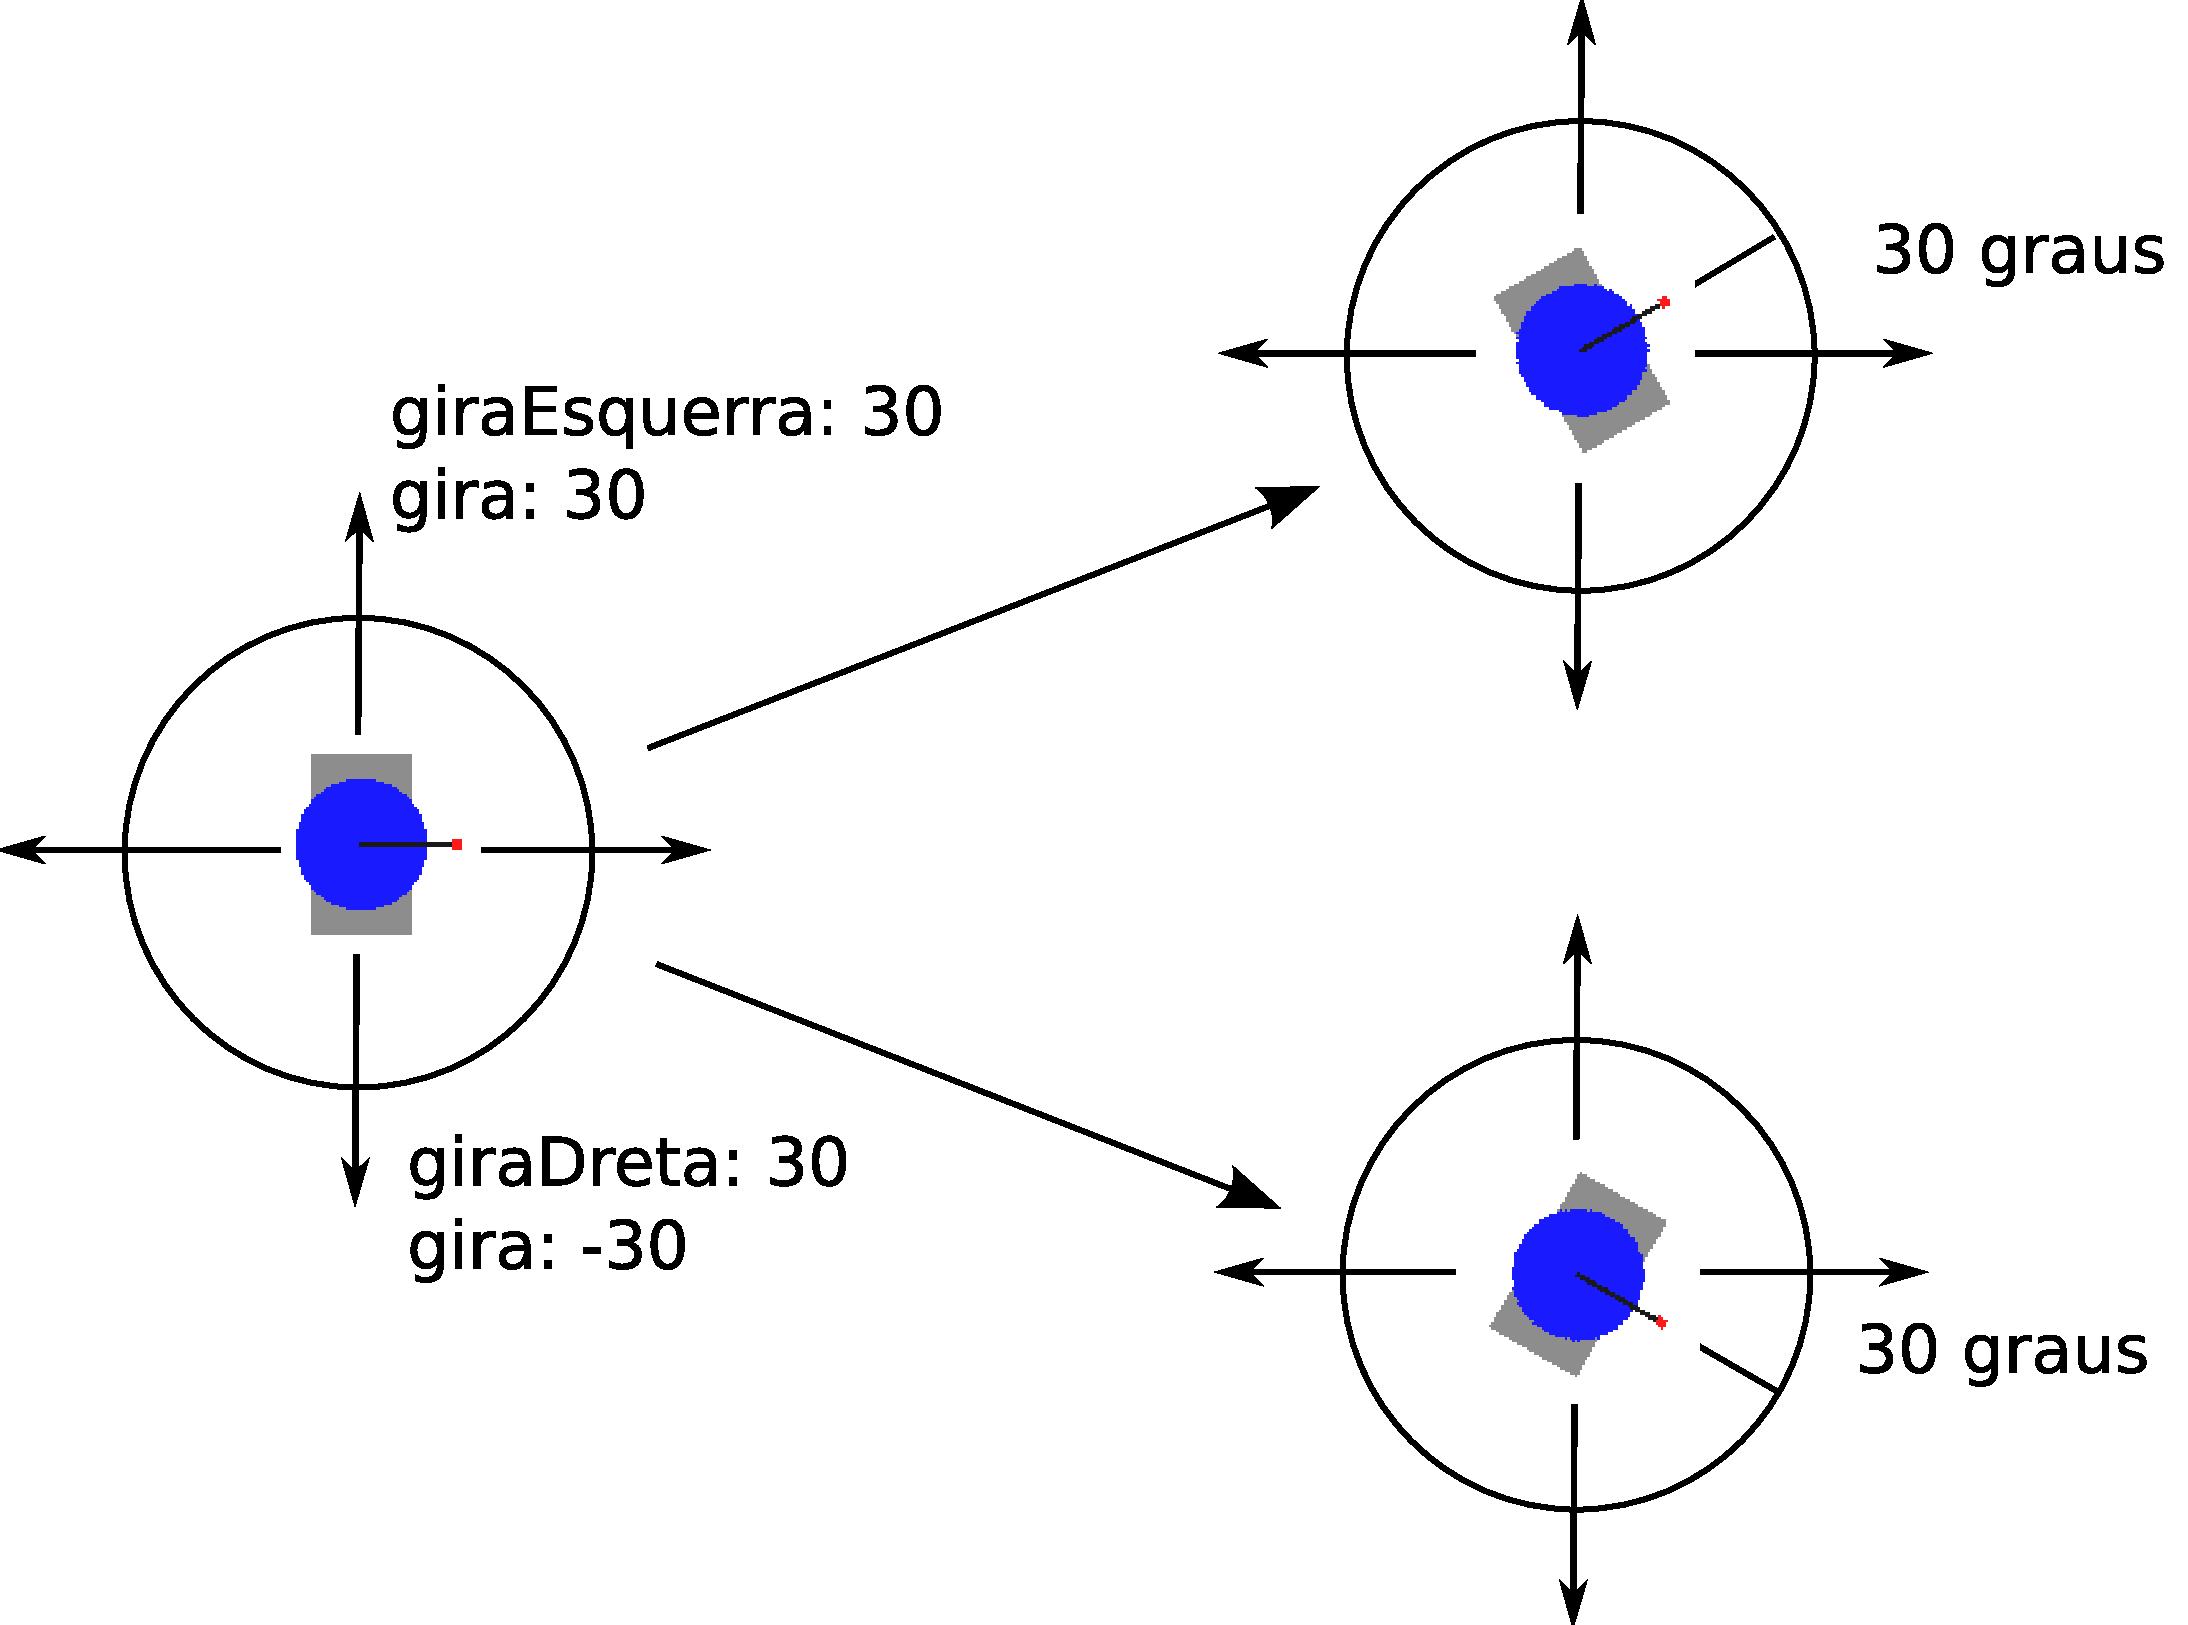
\includegraphics[scale=0.21]{Imatges/figura4-2}
\end{center}
\caption{Girar 30 graus des de la direcció est.}
\label{fig0402}
\end{figure}

\section{Orientació absoluta vs. orientació relativa}
\index{absoluta!orientació, versus orientació relativa|(}
\index{relativa!orientació, versus orientació absoluta|(}
Ja hauríeu de tenir prou confiança en les vostres habilitats manipulant robots com per fer que un robot realitzi qualsevol dibuix compost per línies rectes. Abans de continuar, estigueu segurs que enteneu la diferència entre orientar un robot de manera \emph{absoluta} utilitzant les mètodes \textsf{nord}, \textsf{sud}, \textsf{sudEst}, \textsf{est}, etc., i fer servir els mètodes \textsf{gira:}, \textsf{giraEsquerra:} i \textsf{giraDreta:} per orientar al robot de manera \emph{relativa} a la seva orientació actual. \index{quadrats|seealso{quadrats centrats; quadrats concèntrics}} \index{quadrats!dibuixar}

\noindent
Els experiments 4-2, 4-3 i 4-4 us ajudaran a acabar d'entendre aquesta diferència.

\begin{center}
\colorbox{black}{\makebox[\textwidth]{  \color{white} {\large {\bfseries Experiment 4-2 (un quadrat relatiu)}} }}
\end{center}
\index{quadrat relatiu@un quadrat relatiu, Experiment}
\index{Experiments!quadrat relatiu@un quadrat relatiu}
{\small
\noindent
Escriviu un \emph{script} per dibuixar un quadrat utilitzant el mètode \textsf{giraEsquerra:} o \textsf{giraDreta:}  }
\begin{center}

\includegraphics[height=30mm ,width=30mm]{Imatges/figuraE4-2.jpg}
\end{center}
\noindent
\rule{\textwidth}{3pt}

\begin{center}
\colorbox{black}{\makebox[\textwidth]{  \color{white} {\large {\bfseries Experiment 4-3 (girar el quadrat)} }}}
\end{center}
\index{girar el quadrat, Experiment}
\index{Experiments!girar el quadrat}
{\small
\noindent
Modifiqueu l'experiment anterior afegint la línia \textsf{pica giraEsquerra: 33.} abans de la primera línia contenint el missatge \textsf{ves: 100}. Obtindreu un quadrat altre cop, però aquesta vegada estarà girat 33 graus respecte al que ja havíeu dibuixat.}\\
\noindent
\rule{\textwidth}{3pt}

\begin{center}
\colorbox{black}{\makebox[\textwidth]{  \color{white} {\large {\bfseries Experiment 4-4 (un quadrat trencat)} }}}
\end{center}
\index{quadrat trencat@un quadrat trencat, Experiment}
\index{Experiments!quadrat trencat@un quadrat trencat}
{\small
\noindent
Finalment, executeu l'\emph{script}~\ref{scr4-3}, que intenta dibuixar un quadrat girat utilitzant els mètodes \textsf{nord}, \textsf{sud}, \textsf{est}, i \textsf{oest} que hem introduït al capítol anterior.}\\
\noindent
\rule{\textwidth}{3pt}

\begin{script}  Un quadrat trencat.
\newline
\newline
\noindent

\includegraphics[scale=0.75]{Imatges/figuraS4-3} 
\noindent
\textsf{\upshape
\\
\\$|$ pica $|$\\
pica := Bot nou.\\
{\itshape pica giraEsquerra: 33.}\\
pica ves: 100.\\
pica nord.\\
pica ves: 100.\\
pica oest.\\
pica ves: 100.\\
pica sud.\\
pica ves: 100.\\
}
\label{scr4-3}
\end{script}

Encara obteniu un quadrat? No! El primer costat dibuixat pel robot està tort, mentre que els altres costats són horitzontals o verticals. L'\emph{script} que vau escriure per a l'Experiment 4-3 i l'\emph{Script}~\ref{scr4-3} demostren la diferència tan important que hi ha entre canvis \emph{relatius} i \emph{absoluts} de direcció:

\begin{itemize}
\item Els mètodes \textsf{nord}, \textsf{sud}, \textsf{est}, i \textsf{oest} canvien la direcció d'una manera \emph{absoluta}. La direcció a què el robot acabarà apuntant  \emph{no depèn} de la direcció actual a què està apuntant.
\item Els mètodes \textsf{giraEsquerra:} i \textsf{giraDreta:} canvien la direcció de manera \emph{relativa}. La direcció a què el robot apunta \emph{depèn} de la seva direcció actual.
\end{itemize}

La figura~\ref{fig0403} mostra l'equivalència entre moviments relatius a partir d'un robot que apunta a l'est i moviments absoluts.
Com ja sabeu, aquesta equivalència és només vàlida si el robot està apuntant a l'est i no si està apuntant a qualsevol altra direcció.
Fixeu-vos que girant el robot 180 graus apunta a la direcció oposada; aquest truc s'utilitza sovint als \emph{scripts}.

\begin{figure}[h!]
\begin{center}
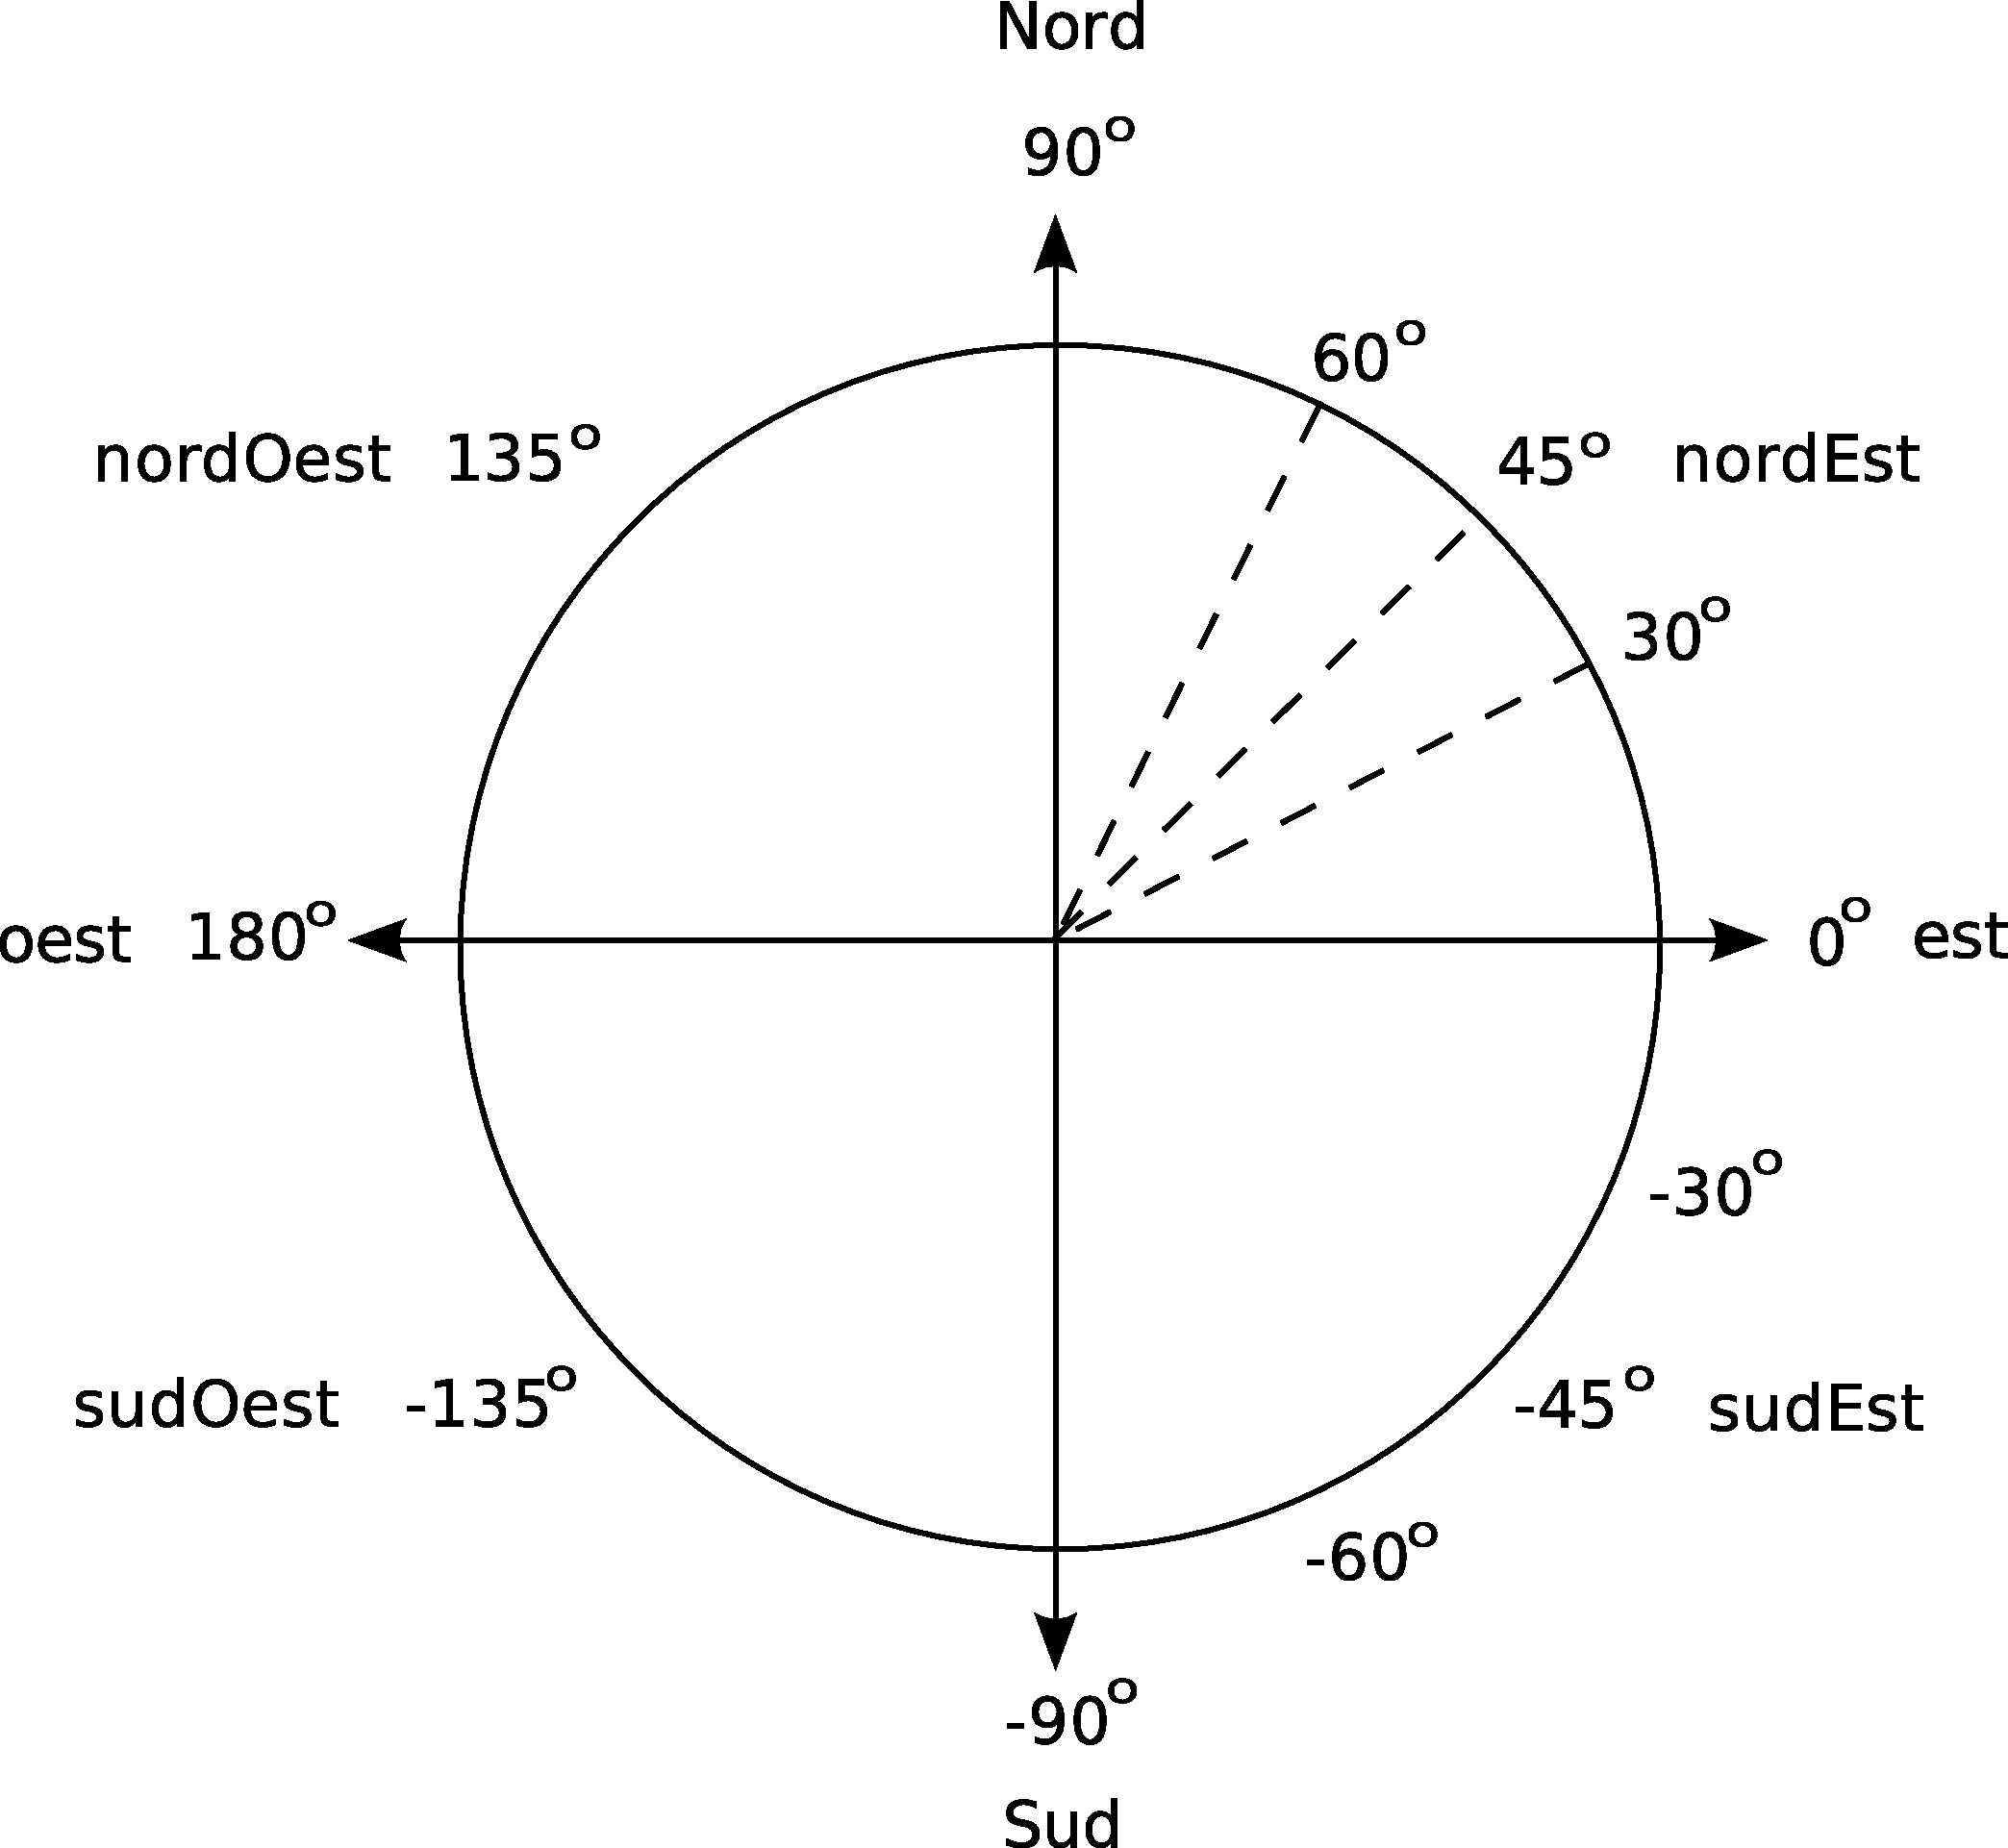
\includegraphics[scale=0.25]{Imatges/figura4-3}
\end{center}
\caption{Comparar l'orientació relativa i absoluta començant per l'est.}
\label{fig0403}
\end{figure}
\index{absoluta!orientació, versus orientació relativa|)}
\index{relativa!orientació, versus orientació absoluta|)}

\section{L'enfocament adequat}
\index{angles!girar|(}
\index{angles!representar}
Un robot nou, com ja sabeu, apunta l'est, és a dir, cap al costat dret de la pantalla. Si demanem al robot que giri a l'esquerra 90 graus, acabarà apuntant al nord. Si li demanem que giri a la dreta 90 graus, apuntarà al sud. L'\emph{Script}~\ref{scr4-4} il·lustra el resultat d'un gir a l'esquerra de 45 graus. Per ajudar-vos a entendre l'\emph{script}, la figura us mostra el punt de partida del robot.
\index{45 graus, girar}

\begin{script}  Jugar amb els angles (1)
\newline
\newline
\noindent
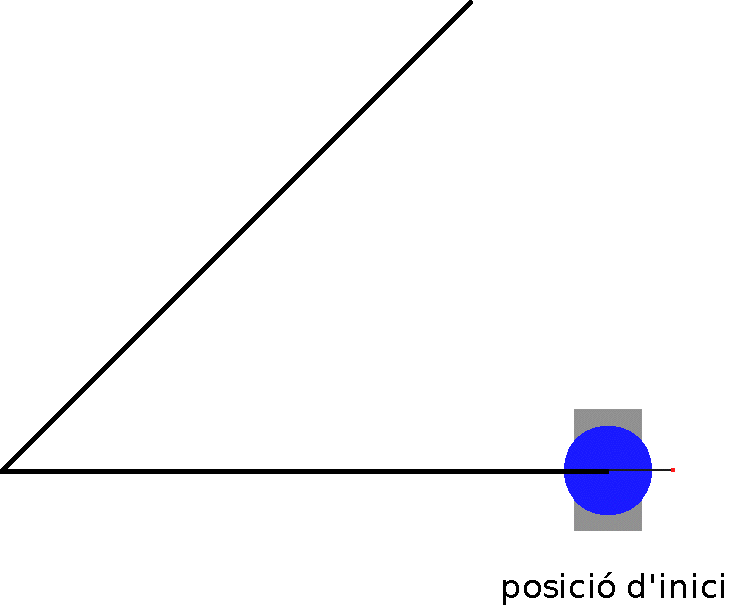
\includegraphics[scale=0.5]{Imatges/figuraS4-4.pdf} 
\noindent
\textsf{\upshape
\\
\\$|$ pica $|$\\
pica := Bot nou.\\
pica oest.\\
pica ves: 100.\\
pica est.\\
pica giraEsquerra: 45.\\
pica ves: 100.\\
}
\label{scr4-4}
\end{script}

La primera part de l'\emph{script}~\ref{scr4-4}, fins a la línia \textsf{pica est}, dibuixa una línia horitzontal, que farà el paper de línia de referència per indicar la direcció est. La darrera part dibuixa una línia en la direcció 45 graus a l'esquerra de la direcció est. Podeu fer variar
el valor de l'angle per veure quina mena d'angles representen altres quantitats en graus. Proveu els valors 60, 120, 180, 240, 360 i 420. En particular, fixeu-vos que un gir de 180 graus és el mateix que tombar el robot per a que apunti a la direcció oposada a la que apuntava. \index{est, indicar la direcció} \index{girar a l'esquerra 45 graus, resultat de}

Veieu alguna diferència entre els arguments 60 i 420? Representen el mateix angle! Qualsevol parell de valors tals que la seva diferència sigui 360 o qualsevol múltiple de 360 són equivalents, ja que 360 graus representen una circumferència completa. Intenteu un angle de 1860 ($1860 = 60 + 360 \times 5$). El resultat és el mateix que obtindríeu amb valors 60 i 420. Així, quan treballeu amb angles recordeu que l'orientació d'un robot no canvia afegint un o més girs complets a aquesta orientació.

Ara provarem de divertir-nos amb el mètode \textsf{giraDreta:}. L'\emph{Script}~\ref{scr4-5} dibuixa les agulles d'un rellotge (l'hora i els minuts) i una línia que ens servirà de referència. Utilitza dos robots, que podeu utilitzar per investigar la correspondència entre els girs a l'esquerra i els girs a la dreta. Hem afegit comentaris entre cometes i hem utiltzat diferents fonts per ajudar-vos a identificar les diverses parts de l'\emph{script}. Fixeu-vos que no heu d'escriure els comentaris, ja que no s'executaran.\index{agulles de rellotge, moure|(} \index{giraDreta: missatge, efecte de|(}

\begin{script}  Jugar amb els angles (2)
\newline
\newline
\noindent
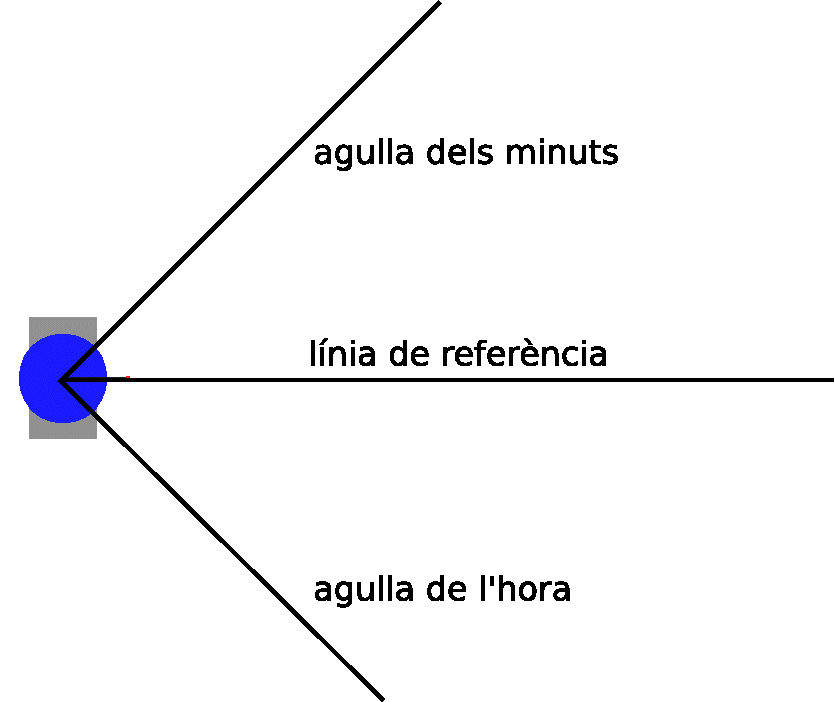
\includegraphics[scale=0.425]{Imatges/figuraS4-5.pdf} 
\noindent
\textsf{\upshape
\begin{tabbing}
\hspace{40mm} \= \kill
\\$|$ pica daly $|$\\
pica := Bot nou.\\
{\itshape pica salta: 200}. \> ``dibuixar la línia de referència''\\
{\itshape pica giraEsquerra: 180}.\\
{\itshape pica ves: 200}.\\
{\itshape pica giraEsquerra: 180}.\\
pica color: Color blau.\\
pica giraEsquerra: 45.\> ``dibuixar l'agulla dels minuts''\\
pica ves: 150.\\
daly := Bot nou.\\
daly color: Color vermell.\\
{\bfseries daly giraDreta: 45}.\>  ``dibuixar l'agulla de l'hora''\\
{\bfseries daly ves: 100}.\\
\end{tabbing}
}
\label{scr4-5}
\end{script}

A l'\emph{Script}~\ref{scr4-5}, el codi en itàlica dibuixa la línia de referència --és a dir, la línia que representa la direcció del robot abans de fer cap gir-- utilitzant el fet que un gir de 180 graus és el mateix que girar per apuntar a la direcció oposada. La línia de referència és també la línia més llarga. Així, encara serà visible si les línies dibuixades pels robots se superposen a la línia de referència. El text en font normal és el codi que dibuixa l'agulla minutera (utilitzant \textsf{pica}) i en negreta, el codi dibuixant l'agulla de l'hora utilitzant el robot \textsf{daly}. \index{angles!canviar els valors dels} \index{agulles de rellotge, moure|)} \index{linies de@línies de referència, dibuixar}

\begin{center}
\colorbox{black}{\makebox[\textwidth]{  \color{white} {\large {\bfseries Experiment 4-5 (moure les agulles del rellotge)} }}}
\end{center}
\index{moure les agulles del rellotge, Experiment}
\index{Experiments!moure les agulles del rellotge}
{\small
\noindent
Experimenteu amb diferents valors dels angles per a cada un dels dos robots; és a dir, canvieu els valors dels angles per als dos mètodes per girar. Després, compareu l'efecte del mètode \textsf{giraEsquerra: 60} (per a  \textsf{pica}) i  \textsf{giraDreta: 300} (per  \textsf{daly}). Podeu veure que girar a l'esquerra 60 graus dóna el mateix resultat que girar a la dreta 300 graus. Això és així ja que la suma dels valors és 360 graus, és a dir, una circumferència sencera.}\\
\noindent
\rule{\textwidth}{3pt}

\vspace*{5mm}

Ara veurem el que passa quan el robot gira a partir d'una altra direcció. Aquí teniu un \emph{script} igual a  l'\emph{script}~\ref{scr4-4}, però aquest cop comencem a girar des del nord. En aquest \emph{script} hem substituït \textsf{daly} per un altre robot, \textsf{berthe}, que 
fa honor a pintor impressionista francés Berthe Morisot.

\vspace*{5mm}

\begin{script}  Jugar amb els angles (3)
\newline
\newline
\noindent
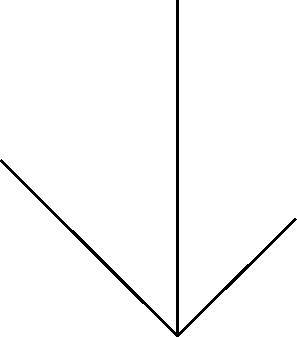
\includegraphics[scale=0.75]{Imatges/figuraS4-6.pdf} 
\noindent
\textsf{\upshape
\\
\\$|$ pica berthe $|$\\
pica := Bot nou.\\
{\bfseries pica nord}.\\
pica salta: 200.\\
pica giraEsquerra: 180.\\
pica ves: 200.\\
pica giraEsquerra: 180.\\
pica color: Color blau.\\
pica giraEsquerra: 45.\\
pica ves: 150.\\
berthe := Bot nou.\\
berthe nord.\\
berthe color: Color vermell.\\
berthe giraDreta: 45.\\
berthe ves: 100.\\
}
\label{scr4-6}
\end{script}

\begin{center}
\colorbox{black}{\makebox[\textwidth]{  \color{white} {\large {\bfseries Experiment 4-6 (canviar la direcció de referència)} }}}
\end{center}
\index{canviar la direcció de referència, Experiment}
\index{Experiments!canviar la direcció de referència}
\index{direcció de referència, canviar}
{\small
\noindent
Continueu experimentant amb  l'\emph{Script}~\ref{scr4-6} canviant la direcció de referència. Per tal que la comparació sigui significativa, haureu d'orientar \textsf{berthe} en la mateixa direcció que \textsf{pica} després de crear-lo. Intenteu qualsevol valor pels angles i proveu de fer prediccions respecte al resultat abans d'executar l'\emph{script}. Continueu experimentant amb l'\emph{script} fins que les vostres prediccions siguin prou acurades.}\\
\noindent
\rule{\textwidth}{3pt}
\newline


Fixeu-vos que sempre hauríeu de ser capaços de predir el que passarà abans d'executar un \emph{script}, ja que l'ordinador executarà totes les instruccions vàlides cegament, incloent-hi les més absurdes.\index{angles!girar|)} \index{giraDreta: missatge, efecte de|)}

\section{Un rellotge robot}
\index{rellotge, crear}
He mencionat abans que les línies dibuixades a l'\emph{Script}~\ref{scr4-6} són similars a les agulles d'un rellotge. L'analogia entre el temps i els angles és una bona analogia, ja que la noció de grau està força correlacionada amb la noció d'hora. Les civilitzacions antigues van descobrir la noció del temps mesurant l'angle del Sol (o d'un estel) relatiu a una direcció de referència. Un \emph{script} com l'\emph{Script}~\ref{scr4-6}, però, us permet posar les agulles del rellotge en una posició que no indica cap moment real del dia. Per exemple, podríeu dibuixar un rellotge amb l'agulla de l'hora apuntant al nord i l'agulla dels minuts apuntant al sud. En canvi, en un rellotge real, si l'agulla dels minuts està apuntant al sud vol dir que ha passat mitja hora des de l'hora en punt i per tant l'agulla de l'hora hauria d'estar a mig camí entre dues hores. \index{angles!versus temps}

Ara estudiareu la relació que hi ha entre l'agulla de l'hora i l'agulla minutera en un rellotge \emph{real} que representa algun moment \emph{real} del dia.

\newpage

\begin{center}
\colorbox{black}{\makebox[\textwidth]{  \color{white} {\large {\bfseries Experiment 4-7 (un rellotge ``real'')} }}}
\end{center}
\index{rellotge real@un rellotge ``real'', Experiment}
\index{Experiments!rellotge real@un rellotge ``real''}
\index{rellotge robot, crear}
\index{temps!versus angles}
{\small
\noindent
Modifiqueu l'\emph{Script}~\ref{scr4-6} de la manera següent:
\begin{itemize}
\item Manteniu la direcció de referència cap al nord (tal com està escrit a l'\emph{Script}~\ref{scr4-6}). Aquesta línia de referència indica les 12:00 del migdia o de la mitjanit.
\item Utilitzeu el mètode \textsf{giraDreta:} per ambdós robots. Després de tot, les agulles del rellotge es mouen en el sentit de les agulles del rellotge, que és cap a la dreta.
\item Ara podem demanar a \textsf{pica} que dibuixi l'agulla minutera multiplicant el nombre de minuts que passen de l'hora que volem indicar per 6 (ja que durant els 60 minuts d'una hora, l'agulla minutera viatja els $6 \times 60 = 360$ graus d'una circumferència sencera). Per exemple, per representar l'agulla minutera per 20 minuts passats de l'hora en punt, hauríeu d'utilitzar l'expressió \textsf{giraDreta: 120} (ja que $120 = 6 \times 20$).
\item Podem demanar \textsf{berthe} que dibuixi l'agulla de l'hora multiplicant el nombre d'hores que volem indicar per 30 (12 hores multiplicat per 30 graus fan 360 graus) afegint mig ($0.5$) grau per cada minut que passi de l'hora en punt, ja que en 60 minuts, l'agulla de l'hora es mou 30 graus. Per exemple, podeu posicionar l'agulla de l'hora a les 2 en punt amb el missatge \textsf{giraDreta: 60} ($60 = 30 \times 2$), mentre que per a les 4:26 cal posicionar l'agulla de l'hora amb el missatge  \textsf{giraDreta: 133} ($133 = 30 \times 4 + 26 \times 0.5$).
\end{itemize}

\noindent
Intenteu dibuixar unes quantes hores i minuts del dia amb aquest \emph{script} modificat.}\\
\noindent
\rule{\textwidth}{3pt}

\section{Dibuixos senzills}
\index{triangles!dibuixar}
Per començar, aquí teniu un \emph{script} per dibuixar un triangle amb tres costats iguals. \index{dibuixar!triangle equilàter} \index{triangle equilàter, dibuixar}

\begin{script}  Un triangle equilàter.
\newline
\newline
\noindent
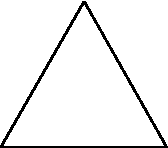
\includegraphics[scale=0.8]{Imatges/figuraS4-7.pdf} 
\noindent
\textsf{\upshape
\\
\\$|$ pica $|$\\
pica := Bot nou.\\
pica ves: 100.\\
pica giraEsquerra: 120.\\
pica ves: 100.\\
pica giraEsquerra: 120.\\
pica ves: 100.\\
pica giraEsquerra: 120.\\
}
\label{scr4-7}
\end{script}

\noindent
La darrera línia de codi no és necessària per dibuixar el triangle; serveix per apuntar \textsf{pica} altra cop cap a l'est (la seva posició inicial).

\vspace*{2mm}

\noindent
Ara, ja esteu preparats per dibuixar una casa.\index{casa, dibuixar}

\begin{center}
\colorbox{black}{\makebox[\textwidth]{  \color{white} {\large {\bfseries Experiment 4-8} }}}
\end{center}
\index{dibuixar!una casa}
{\small
\noindent
Dibuixeu una casa tal com es mostra a la figura. Intenteu dibuixar cases de diferentes formes.}
\begin{center}

\includegraphics[scale=0.75]{Imatges/figuraE4-8.pdf} 
\end{center}
\noindent
\rule{\textwidth}{3pt}

\section{Polígons regulars}
\index{dibuixar!polígons regulars}
\index{poligon@polígon!dibuixar|(}
\index{poligon regular@polígon regular!dibuixar|(}
Un polígon regular és una figura composta per segments de línia tots de la mateixa longitud i tots els angles de la qual són iguals. Un triangle equilàter és un polígon regular amb tres costats. Un quadrat és un polígon regular amb quatre costats. Per exemple, l'\emph{Script}~\ref{scr4-7} dibuixa un triangle equilàter de costats de mida 100 píxels. S'obté dient-li a \textsf{pica} d'anar endavant 100 píxels i girar a la dreta 120 graus, i repetir aquests dos missatges dues vegades més, de manera que en total són executats tres vegades.

Podeu programar un robot per dibuixar un polígon regular amb qualsevol nombre de costats demanant-li que es mogui una certa quantitat de píxels i després giri a l'esquerra o a la dreta 360 graus dividit pel nombre de costats del polígon; aquesta seqüència s'ha de repetir tantes vegades com costats tingui el polígon. Fixeu-vos que el darrer gir del robot no cal que el posem, ja que el robot ja ha dibuixat l'última línia del polígon.

\begin{center}
\colorbox{black}{\makebox[\textwidth]{  \color{white} {\large {\bfseries Experiment 4-9} }}}
\end{center}
\index{dibuixar!pentàgon}
{\small
\noindent
Dibuixeu un pentàgon regular (un polígon regular amb cinc costats), tal com es mostra a la figura, amb costats de 100 píxels.}
\begin{center}
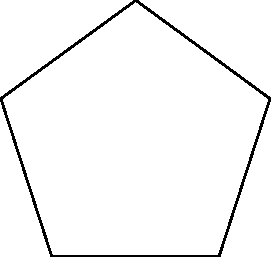
\includegraphics[scale=0.9]{Imatges/figuraE4-9.pdf}
\end{center}
\noindent
\rule{\textwidth}{3pt}

\begin{center}
\colorbox{black}{\makebox[\textwidth]{  \color{white} {\large {\bfseries Experiment 4-10} }}}
\end{center}
\index{dibuixar!hexàgon}
\index{hexàgons!dibuixar}
{\small
\noindent
Dibuixeu un hexàgon regular (un polígon regular amb sis costats), tal com es mostra a la figura, amb costats de 100 píxels.}
\begin{center}

\includegraphics[scale=0.8]{Imatges/figuraE4-10.pdf} 
\end{center}
\noindent
\rule{\textwidth}{3pt}
\newline

Si teniu prou curiositat per veure fins a on podeu arribar en aquest procés, podeu utilitzar les possibilitats de tallar i enganxar de l'\textsf{Espai de Treball Bot} per generar polígons regulars d'un gran nombre de costats. Si voleu, aneu incrementant el nombre de costats. Al capítol~\ref{cap7}, 
us ensenyarem com podeu escriure una seqüència d'expressions i fer que es repeteixi tantes vegades com vulgueu. \index{tallar i enganxar, generar polígons regulars amb} \index{poligon@polígon!dibuixar|)} \index{poligon regular@polígon regular!dibuixar|)}

\begin{center}
\colorbox{black}{\makebox[\textwidth]{  \color{white} {\large {\bfseries Experiment 4-11}} }}
\end{center}
\index{tres radis, dibuixar figura amb}
{\small
\noindent
Dibuixeu aquesta figura amb tres radis.}
\begin{center}
\includegraphics[scale=0.75]{Imatges/figuraE4-11.pdf} 
\end{center}
\noindent
\rule{\textwidth}{3pt}

\section{Resum}

\begin{itemize}
\item Un robot es pot orientar \emph{relativament} a la seva direcció actual amb els mètodes \textsf{giraEsquerra:} i \textsf{giraDreta:}.
\item El paràmetre que cal proporcionar als mètodes \textsf{giraEsquerra:} i \textsf{giraDreta:} es dóna en graus.
\item Girar 360 graus correspon a girar una circumferència sencera
\item Girar 180 graus correspon a girar mitja circumferència.
\item Els angles els valors dels quals difereixen en algun múltiple de 360 graus són equivalents.
\end{itemize}

\newpage

\noindent
Aquí teniu la llista de mètodes que heu après en aquest capítol.\index{tornarInvisible i tornarVisible mètodes, efectes de} \index{direcció!canviar de} \index{receptors!amagar i mostrar} \index{robots!canviar la direcció dels}

\vspace*{5mm}
\noindent
\setlength{\extrarowheight}{1mm}
{\small \begin{tabular}{p{18mm}p{38mm}p{45mm}p{30mm}}
\hline
\textbf{Mètode} & \textbf{Sintaxi} & \textbf{Descripció} & \textbf{Exemple}\\
\hline
\textsf{giraEsquerra:} & \textsf{giraEsquerra: unNombre} &
Demana al robot que canviï la seva direcció un determinat nombre de graus a l'esquerra.
& \textsf{pica giraEsquerra: 30} \\
\textsf{giraDreta:} & \textsf{giraDreta: unNombre} &
Demana al robot que canviï la seva direcció un determinat nombre de graus a la dreta.
& \textsf{pica giraDreta: 30} \\
\textsf{gira:} & \textsf{gira: unNombre} &
Demana al robot que canviï la seva direcció un determinat nombre de graus, seguint la convenció matemàtica que ens diu que un nombre positiu representa un gir a l'esquerra i un nombre negatiu representa un gir a la dreta.
& \textsf{pica gira: 30} \\
\textsf{tornarInvisible} & \textsf{tornarInvisible} &
Amaga el receptor
& \textsf{pica tornarInvisible} \\
\textsf{tornarVisible} & \textsf{tornarVisible} &
Mostra el receptor
& \textsf{pica tornarVisible} \\
\hline
\end{tabular}}

\chapter{L'entorn de Pica}
\label{cap5}

En aquest capítol us presentarem l'entorn de pica, us ensenyarem com utilitzar les eines disponibles i a guardar els vostres \emph{scripts}. També retornarem a la noció de missatge i us ensenyarem que no només podeu demanar a l'entorn que executi un missatge, sinó que a més li podeu demanar que escrigui el \emph{resultat} de l'execució del missatge.

\section{El menú principal}
\index{menu@menú principal, opcions del}
Quan feu clic al fons de l'entorn obteniu el menú principal, com podeu veure a la figura~\ref{fig0501}.

\begin{figure}[h]
\begin{center}
\includegraphics[scale=0.5]{Imatges/figura5-1}
\end{center}
\caption{Opcions del menú de l'entorn}
\label{fig0501}
\end{figure}

Si voleu saber què fa una determinada opció del menú, mogueu el punter del ratolí sobre l'opció durant un segon i voilà!  apareixerà una bafarada que descriu l'opció. El menú principal dóna accés a cinc grans grups de funcionalitats: l'accés a eines, les captures de pantalla, l'accés a alguns comportaments dels robots, l'aspecte i guardar l'entorn. Els submenús estan agrupats de la següent manera:\index{aspecte\dots submenú, descripció de} \index{accions BotsInc\dots submenú, descripció de} \index{obre\dots submenú, descripció de} \index{submenú, explicació de}

\begin{itemize}
\item El menú \textbf{obre\dots} recull diverses eines com ara l'explorador del codi dels robots, l'\textsf{Espai de Treball Bot}, un explorador de fitxers i altres eines que anirem veient a mida que les necessitem.
\item El menú \textbf{accions BotInc\dots} recull diverses accions com per exemple indicar quina versió de l'entorn estem utilitzant o esborrar tots els robots i les seves traces, també n'inclou d'altres per reinstal·lar l'entorn si cal: reinstal·lar les preferències per defecte assigna els valors per defecte a les preferències que poguéssiu haver modificat amb el menú d'aspecte.
\item El menú \textbf{aspecte\dots} recull accions que canvien l'aspecte de l'entorn, com canviar les fonts utilitzades, activar el mode de pantalla completa o modificar color del fons de l'entorn.
\end{itemize}

\subsection{Obtenir un \textsf{Espai de Treball Bot}}
\index{editor de text Espai de Treball Bot!obtenir|(}
Si tanqueu l'\textsf{Espai de Treball Bot} per accident no us amoïneu. Podeu obtenir-ne un de nou a partir de la solapa blava, tal com es mostra a l'esquerra de la figura~\ref{fig0502}, o a partir del menú del Món, com veiem a la figura~\ref{fig0501}. Per instal·lar un nou \textsf{Espai de Treball Bot} a la solapa de Treball, obriu-la (la solapa que està situada a la part de sota) i arrossegueu l' \textsf{Espai de Treball Bot} des de la solapa blava fins a la solapa de Treball.\index{solapa!obtenir Espai de Treball Bot}
\begin{figure}[h]
\begin{center}
\includegraphics[scale=1.65]{Imatges/figura5-2.png}
\end{center}
\caption{Obtenir un nou \textsf{\upshape Espai de Treball Bot} a partir de les solapes.}
\label{fig0502}
\end{figure}

La solapa blava conté altres eines que utilitzarem més endavant. La segona eina és bàsicament un explorador de codi que utilitzareu quan comenceu a definir nous mètodes per als robots.\index{menu@menú, opcions del; explicacions}

L'entorn conté una eina senzilla (figura~\ref{fig0503}) que llista els missatges més importants que un robot pot entendre. Podeu accedir-hi via el menú \textbf{obrir... vocabulari} o el menú d'\textbf{ajuda} (opció \textbf{obre vocabulari}). La finestra del vocabulari llista els missatges, agrupats d'acord al seu tipus. Per exemple, els missatges \textsf{est}, \textsf{nord} i similars estan llistats sota \textbf{direccions absolutes}.\index{editor de text Espai de Treball Bot!obtenir|)} \index{vocabulari, subfinestra; llistar missatges a la}

\section{Interaccionar amb Squeak}
\index{halo de nanses!explicació|(}
\index{missatges!exemples comuns de}
\index{Squeak!interaccionar amb|(}
La interacció amb Squeak està basada en la suposició que teniu un ratolí de tres botons, tot i que hi ha equivalències per a ratolins de dos botons (Windows) o d'un sol botó (Mac), com mostrem a la taula~\ref{tab0501}. Cada botó està associat amb un cert conjunt d'operacions. El botó esquerre serveix per obtenir menus contextuals i per apuntar i seleccionar, el botó del mig és per  manipular finestres (fer que una finestra estigui davant de tot o per moure una finestra), i el botó dret és per obtenir \emph{nanses}\footnote{\emph{Nota del Traductor:} No sé encara com traduir \emph{handle} d'una manera satisfactòria, però segons el TERMCAT \emph{nansa} és la traducció correcta en Informàtica.}, que són petites icones rodones que apareixen al voltant dels elements gràfics (veure figura~\ref{fig0504}). Col·lectivament, les nanses s'anomenen un \emph{halo}. Les nanses són útils ja que permeten que l'usuari interaccioni directament amb el robot. Els introduirem en detall al proper capítol.\index{botons del ratolí, operacions associades als} \index{tecles, combinacions i botons del ratolí, explicacions} \index{botó esquerre del ratolí, conjunt d'operacions associades amb} \index{botó central del ratolí, conjunt d'operacions associades amb} \index{botó dret del ratolí, conjunt d'operacions associades amb} \index{botons del ratolí!explicació|(} \index{botons del ratolí!i combinacions de tecles} \index{Apuntar i Seleccionar amb el ratolí} \index{Squeak!interaccionar amb|)}
\noindent
\begin{table}[h!]
\caption{Combinacions amb tecles i botons del ratolí}
\label{tab0501}
\begin{center}
{\small \begin{tabular}{p{30mm}p{40mm}p{30mm}p{30mm}}
\hline
&{\small \textbf{Apuntar i Seleccionar}} & {\small \textbf{Menus Sensibles al Context}} & {\small \textbf{Obrir l'Halo}}\\
\hline
{\small Tres botons} & {\small clic esquerre} & {\small clic central} & {\small clic dret}\\
{\small Windows: 2 botons} & {\small clic esquerre} & {\small \emph{Alt} - clic esquerre} & {\small clic dret}\\
{\small Mac: 1 botó} & {\small clic} & {\small \emph{Option} - clic} & {\small \emph{Command} - clic} \\
\hline
\end{tabular}}
\end{center}
\end{table}

\newpage

\begin{figure}[h!]
\begin{center}
\includegraphics[scale=2]{Imatges/figura5-3.png}
\end{center}
\caption{Els missatges més importants per als robots.}
\label{fig0503}
\end{figure}

\begin{figure}[h!]
\begin{center}
\includegraphics[scale=0.5]{Imatges/figura5-4}
\end{center}
\caption{Fent clic amb el botó de la dreta apareix l'halo.}
\label{fig0504}
\end{figure}

\newpage

\section{Utilitzar l'\textsf{Espai de Treball Bot} per guardar un \emph{script}}
\index{scripts@\emph{scripts}!guardar amb l'Espai de Treball Bot}
\index{guardar el contingut, opció del menú, accedir}
\index{botons del ratolí!explicació|)}
\index{editor de text Espai de Treball Bot!guardar \emph{scripts} amb}
\index{halo de nanses!explicació|)}
\index{Fes-ho tot (botó), efecte de}
\index{Fes-ho (botó), efecte de}
\index{Eliminar camins (botó), efecte de}
\index{Eliminar Bots (botó), efecte de}
\index{Eliminar-ho tot (botó), efecte de}
\index{seleccionar amb el ratolí}
L'\textsf{Espai de Treball Bot} té cinc botons i un menú que us permet guardar \emph{scripts}. El botó \textbf{Fes-ho tot} executa tot l'\emph{script} contingut en l'espai de treball. El botó \textbf{Fes-ho} executa el tros seleccionat de l'\emph{script} dins l'espai de treball. El botó \textbf{Eliminar Camins} esborra els camins dibuixats pels robots sense esborrar els robots. El botó \textbf{Eliminar Bots} esborra només els robots sense eliminar els camins. El botó \textbf{Eliminar-ho tot} esborra els robots i els camins.

Un cop heu escrit un \emph{script}, pot ser que vulgueu guardar-lo en un fitxer, per, si cal, tornar-lo a utilitzar. L'\textsf{Espai de Treball Bot} us permet guardar i carregar fitxers via el menú de l'espai de treball. Feu clic dins l'espai de treball per fer aparèixer el menú associat, tal com podeu veure a la figura~\ref{fig0505}. L'opció \textbf{guardar el contingut} guardarà tot el contingut de l'espai de treball en un fitxer.
Triar aquesta opció fa que aparegui una finestra de diàleg, com veieu a la figura. Fixeu-vos que els sistema comprova si ja existeix algun fitxer amb el mateix nom. Si és així, el sistema us dóna l'opció de sobreescriure el fitxer o guardar-lo amb un altre nom. \index{menu@menús contextuals, accedir a}

\begin{figure}[h]
\begin{center}
\includegraphics[height=30mm ,width=123mm ]{Imatges/figura5-5.png}
\end{center}
\caption{\emph{Esquerra:} Opcions del menú de l'\textsf{\upshape Espai de Treball Bot}.
 	\emph{Mig:} Especifiquem el nom del fitxer en què volem guardar l'script.
	\emph{Dreta:} Si el fitxer ja existeix, podeu sobreescriure'l o reanomenar-lo.}
\label{fig0505}
\end{figure}

\section{Carregar un \emph{script}}
\index{llista de fitxers (\emph{file list}), carregar \emph{scripts} amb}
\index{scripts@\emph{scripts}!carregar}
Per carregar un \emph{script}, heu de fer servir una llista de fitxers (\emph{file list}), una eina que us permet seleccionar i carregar fitxers diferents dins Squeak. Podeu obtenir la llista de fitxers seleccionant l'opció \textbf{obre... fitxers} a partir del menú principal. Una llista de fitxers conté diverses subfinestres. La finestra de dalt a l'esquerra us permet explorar discos i carpetes; cada vegada que seleccioneu una opció d'aquesta finestra, la finestra de dalt a la dreta s'actualitza. Mostra tots els fitxers continguts a la carpeta seleccionada dins la finestra de l'esquerra. Quan trieu un fitxer de la finestra de la dreta, la finestra de baix automàticament mostra el seu contingut. La figura~\ref{fig0506} mostra que estem a la carpeta \textsf{ReadyMac}, dins la qual hem seleccionat el fitxer \textsf{quadrat.text}.\index{carpetes, explorar}

\begin{figure}[h]
\begin{center}
\includegraphics[scale=0.65]{Imatges/figura5-6}
\end{center}
\caption{La llista de fitxers està oberta a l'script \textsf{\upshape quadrat.text}.}
\label{fig0506}
\end{figure}

Per carregar un \emph{script}, senzillament heu de copiar el contingut de la finestra de baix utilitzant l'opció del menú \textbf{copy}\footnote{\emph{Nota del Traductor:} La llista de fitxers (\emph{file list}) és una eina de l'entorn Squeak general, no de l'entorn dels bots, per això ni l'eina ni els seus menus han estat traduïts.} i enganxar-la dins l'\textsf{Espai de Treball Bot} utilitzant l'opció \textbf{enganxar}, tal com faríeu amb qualsevol editor de text.

\section{Capturar un dibuix}
\index{capturar pantalla (opció menú), accedir|(}
\index{dibuixar!capturar|(}
Per guardar els vostres dibuixos, podeu utilitzar la possibilitat de capturar la pantalla del vostre ordinador. Amb alguns ordinadors això és problemàtic. Per evitar aquests problemes, l'entorn us ofereix un mecanisme simple per capturar la pantalla, tant se val amb quin ordinador treballeu. Obriu el menú principal fent clic al fons de l'entorn. El menú ofereix dues opcions per capturar pantalles, anomenats \textbf{captura pantalla} i \textbf{captura i guarda imatge}, tal i com es mostra a la figura~\ref{fig0507}.

\begin{figure}[h]
\begin{center}
\includegraphics[height=40mm ,width=80mm ]{Imatges/figura5-7.png}
\end{center}
\caption{\emph{Esquerra:} Dues possibilitats per capturar i guardar el dibuix.
	\emph{Dreta:} El cursor ha canviat i indica que Squeak està preparat per a la captura. Ara feu clic per indicar una cantonada de la regió rectangular que voleu capturar.}
\label{fig0507}
\end{figure}

L'opció més senzilla de les dues és utilitzar  \textbf{captura i guarda imatge}. Quan seleccioneu aquesta opció, Squeak mostra que està preparat per capturar una imatge canviant la forma del cursor al dibuix d'una cantonada, com es veu a la dreta de la figura~\ref{fig0507}. Poseu el cursor en una cantonada de la regió rectangular que voleu capturar, feu clic, i arrossegueu el ratolí per delimitar la regió desitjada. La imatge de la regió es mostrarà a la cantonada superior esquerra de la finestra d'Squeak i Squeak us demanarà el nom sense extensió que ha de donar al fitxer. \index{captura i guarda imatge, opció del menú, accedir|(}

Si voleu capturar una regió de la pantalla, utilitzeu l'opció \textbf{captura pantalla}. En aquest cas, Squeak no us demanarà guardar el fitxer, enlloc d'això us permetrà capturar una regió de la pantalla, mostrant-la a la cantonada superior esquerra de l'entorn. Ara, podeu manipular aquesta imatge utilitzant l'halo que obteniu fent clic sobre la imatge amb el botó dret del ratolí. Un cert nombre de nanses apareixen al voltant de la imatge, com veieu a l'esquerra de la figura~\ref{fig0508}. Ara podeu fer clic damunt de la nansa vermella, i s'obrirà la possibilitat de fer un cert conjunt d'accions sobre la vostre imatge\footnote{\emph{Nota del Traductor:} Altre cop, el menú de l'halo és una eina de l'entorn Squeak general, no de l'entorn dels bots, per això no ha estat traduït}. Trieu \textbf{export...} i Squeak us demanarà en quin format voleu guardar la imatge. Llavors, Squeak us demanarà pel nom del fitxer. Fixeu-vos que podeu importar aquests fitxers dins Squeak arrossegant-los des de l'escriptori de l'ordinador.\index{capturar pantalla (opció menú), accedir|)} \index{fitxers!importar} \index{halo de nanses!accedir}\index{halo de nanses!obtenir en dibuixar robots} \index{importar fitxers} \index{captura i guarda imatge, opció del menú, accedir|)} \index{pantalla, capturar regions de la}

\begin{figure}[t]
\begin{center}
\includegraphics[scale=3]{Imatges/figura5-8.png}
\end{center}
\caption{Obriu l'halo i trieu l'opció \textbf{\upshape export...} del menú de la nansa vermella per guardar la imatge a disc.}
\label{fig0508}
\end{figure}

\section{Resultat dels missatges}
\index{Smalltalk!comportament dels objectes a}
\index{dibuixar!capturar|)}
\index{missatges!resultats dels}
\index{objectes!comportament a Smalltalk}
\index{resultats d'un missatge, significat de}
A Smalltalk els objectes només es comuniquen enviant i rebent missatges a i des d'altres objectes. Un cop un objecte rep un missatge, l'executa, i, addicionalment, retorna  un resultat. Un resultat és un objecte que l'objecte receptor retorna a l'objecte que ha enviat el missatge. La comunicació entre objectes mitjançant missatges és similar a la comunicació entre persones mitjançant cartes: Algunes cartes ens poden exigir la realització d'alguna acció (com un avís de l'ajuntament que hem de pagar l'impost de circulació), mentre que altres cartes no les podrem rebre sense una signatura de conformitat (una carta certificada).

A Squeak, el receptor d'un missatge sempre retorna un resultat, que per defecte és el receptor del missatge. Sovint, però, aquest resultat no és gaire interessant. Per exemple, enviar el missatge \textsf{ves: 100} a un robot fa que el robot es mogui 100 píxels en la seva direcció actual. No en fem res del resultat retornat , que és el mateix robot, de manera que en aquest cas ignorem el resultat retornat. En molts casos el resultat de l'execució és important. Per exemple, l'expressió \textsf{2 + 3} envia el missatge \textsf{+ 3} a l'objecte \textsf{2}, que retorna l'objecte \textsf{5}. Enviar el missatge \textsf{color} a un robot retorna el seu color actual. El resultat d'un missatge pot ser utilitzat en un altre missatge, formant part d'un missatge compost. Per exemple, quan l'expressió \textsf{(2 + 3) * 10} s'executa, l'expressió \textsf{(2 + 3)} s'executa enviant el missatge \textsf{+ 3} a l'objecte \textsf{2} i retornant \textsf{5}. El resultat \textsf{5} és utilitzat com l'objecte a què un segon missatge \textsf{* 10} és enviat. Així, \textsf{5} és el receptor del missatge, i retorna com a resultat \textsf{50}.

L'entorn Squeak us permet executar missatges sense haver de tractar amb el resultat del missatge, però també us permet executar missatges i escriure el valor retornat per l'enviament del missatge. La propera secció il·lustrarà amb detalls aquesta diferència.

\vspace*{5mm}

\noindent
\rule{\textwidth}{2pt}
\noindent
\textbf{Nota} Un \emph{resultat} és un objecte que l'objecte receptor retorna a l'objecte que li ha enviat un missatge. Per exemple, \textsf{2 + 5} retorna \textsf{7} i \textsf{pica color} retorna el color de \textsf{pica}, un objecte color.
\noindent
\rule{\textwidth}{2pt}

\newpage

A la figura~\ref{fig0509}, l'expressió \textsf{50 + 90} se selecciona, després s'executa utilitzant el menú i el resultat, \textsf{140}, s'escriu a la pantalla.
\begin{figure}[h!]
\begin{center}
\includegraphics[height=40mm ,width=110mm ]{Imatges/figura5-9.png}
\end{center}
\caption{
\emph{Esquerra:} Seleccionar l'expressió \textsf{\upshape 50 + 90}.
\emph{Mig:} Obrir el menú.
\emph{Dreta:} Executar el missatge i escriure el resultat.
}
\label{fig0509}
\end{figure}

\section{Executar un \emph{script}}
\index{scripts@\emph{scripts}!executar|(}
Hi ha tres maneres d'executar un \emph{script}.

\begin{enumerate}
\item Utilitzant els botons de l'editor de l'\textsf{Espai de Treball Bot}. Al capítol~\ref{cap2} vau veure una manera senzilla d'executar el vostre primer \emph{script} tot prement el botó \textbf{Fes-ho tot} de l'\textsf{Espai de Treball Bot}. Però per executar un \emph{script}, també podeu \emph{seleccionar} amb el ratolí el text que voleu executar (la selecció es torna de color verd) i prémer el botó \textbf{Fes-ho} de l'\textsf{Espai de Treball Bot}.
\item Utilitzant el menú. Seleccioneu el tros de l'\emph{script} que voleu executar, com veieu a la figura~\ref{fig0510}. Obriu el menú fent clic amb el botó del mig del ratolí (o prement la tecla \emph{option} mentre feu clic amb el botó esquerre), i trieu l'opció \textbf{fes-ho (d)} o l'opció \textbf{escriu-ho (p)} del menú, com heu vist a la figura~\ref{fig0509}.\index{fes-ho (d) missatge, efecte de} \index{escriu-ho (p) opció menú, seleccionar} \index{scripts@\emph{scripts}!seleccionar el text complet de} \index{paraules, seleccionar en un \emph{script}}
\begin{figure}[h]
\begin{center}
\includegraphics[height=65mm ,width=90mm ]{Imatges/figura5-10.png}
\end{center}
\caption{Seleccionar un tros d'un script i executar-lo explícitament utilitzant el menú}
\label{fig0510}
\end{figure}
\item Utilitzant les tecles de drecera. Seleccioneu un fragment del text, després premeu command+D en un Mac o alt+D en un PC.
\end{enumerate}

\subsection{Consells}

Per seleccionar automàticament tot el text d'un \emph{script}, podeu fer clic al començament del text (abans del primer caràcter), al final del text o a la línia següent a la darrera expressió. Si voleu seleccionar una paraula, podeu fer doble clic a qualsevol lloc de la paraula. Si voleu seleccionar una línia, feu doble clic al començament (abans del primer caràcter) o al final (després del darrer caràcter) de la línia.

\subsection{Dos exemples}
\index{colors!demanar a un robot|(}
\index{robots!determinar els colors dels|(}
\index{pica color, expressió; executar|(}
Quan executeu l'expressió \textsf{pica color} utilitzant l'opció \textbf{fes-ho (d)} del menú, el missatge \textsf{color}, que demana al robot el seu color, és enviat i executat. La sensació que fa, però, és que no ha passat res. Això és perquè no heu demanat al sistema que faci alguna cosa amb el resultat de l'execució del missatge. Si esteu interessats en el resultat del missatge, hauríeu de fer servir l'opció del menú \textbf{escriu-ho (p)}, com veieu a la figura~\ref{fig0511}. Això provoca que s'executi el fragment de codi seleccionat \emph{i} que s'escrigui el resultat del darrer missatge del codi. A la figura l'expressió \textsf{Bot nou} s'executa i el missatge \textsf{color} s'envia al nou robot tot just creat. El missatge \textsf{color} s'executa i el color del robot receptor és retornat i escrit, com es mostra a la figura~\ref{fig0512}. El text (\textsf{TranslucentColor r: 0.0 g: 0.0 b: 1.0 alpha: 0.847}) ens diu que el color del robot és un color transparent amb tres components de color, vermell (\textsf{r} de \emph{red}), verd (\textsf{g} de \emph{green}) i blau (\textsf{b} de \emph{blue}).\index{expressió Bot nou, executar} \index{color, missatges!executar} \index{colors!demanar a un robot|)} \index{pica color, expressió; executar|)} \index{robots!determinar els colors dels|)}

\begin{figure}[h!]
\begin{center}
\includegraphics[height=60mm ,width=115mm ]{Imatges/figura5-11.png}
\end{center}
\caption{Obriu el menú i trieu l'opció \textbf{\upshape escriu-ho (p)} per executar el fragment de codi seleccionat i escriure el resultat retornat.}
\label{fig0511}
\end{figure}

\begin{figure}[h!]
\begin{center}
\includegraphics[height=30mm ,width=122mm ]{Imatges/figura5-12.png}
\end{center}
\caption{El resultat del missatge s'escriu com una representació textual d'un color.}
\label{fig0512}
\end{figure}

Anem a fer una ullada a un exemple final per assegurar-nos que heu entès quan heu d'utilitzar \textbf{escriu-ho (p)}. Quan executeu l'expressió \textsf{100 + 20} utilitzant l'opció \textbf{fes-ho (d)} del menú, el missatge \textsf{+ 20} s'envia a l'objecte  \textsf{100}, al que se suma  \textsf{20}. Tot i així, no veieu res. Això és normal, ja que en aquest cas l'execució del missatge  \textsf{+ 20} retorna un nou nombre representant la suma, però no heu demanat a Squeak que l'escrigui. Per veure el resultat, heu d'escriure el resultat de l'execució del missatge utilitzant l'opció \textbf{escriu-ho (p)} del menú. A partir d'ara, escriurem ``\textsf{-- Escriure el valor retornat:}'' per indicar que estem utilitzant la comanda d'escriure per executar una expressió i escriure'n el resultat, com veieu a l'\emph{script}~\ref{scr5-1}. Fixeu-vos que utilitzarem aquesta convenció només si el resultat és important. \index{expressions!escriure els resultats de} \index{halo de nanses!accedir} \index{escriure!resultat d'una expressió} \index{scripts@\emph{scripts}!executar|)}

\begin{script}  Escriure el resultat d'executar una expressió.
\noindent
\textsf{\upshape
\\
\\
(100 + 20) * 10\\
{\itshape -- Escriure el valor retornat:} 1200\\
}
\label{scr5-1}
\end{script}

\noindent
\rule{\textwidth}{2pt}
\noindent
\textbf{Important!}  Hi ha dues maneres d'executar una expressió: (1) utilitzant l'opció \textbf{fes-ho (d)} del menú per executar una expressió,
i (2) utilitzant l'opció \textbf{escriu-ho (p)} del menú per executar i escriure el resultat retornat.\\
\noindent
\rule{\textwidth}{2pt}

\section{Resum}
\index{expressions!executar}
\index{robots!moure}
\index{halo de nanses!aconseguir-ne informació}
\begin{itemize}
\item Per executar una expressió, selecciona un bocí de text representant una o diverses expressions i prem el botó \textbf{Fes-ho} o selecciona l'opció \textbf{fes-ho (d)} del menú d'execució.
\item Un resultat és un objecte que s'obté d'un missatge. Per exemple, \textsf{pica color} retorna el color del robot.
\item Hi ha dues maneres d'executar una expressió, (1) utilitzant l'opció \textbf{fes-ho (d)} del menú per executar una expressió,
i (2) utilitzant l'opció \textbf{escriu-ho (p)} del menú per executar i escriure el resultat retornat.
\end{itemize}

\chapter{Divertim-nos amb els robots}
\label{cap6}


\begin{figure}[h]
\includegraphics[height=50mm ,width=87mm ]{Imatges/figura6-0.png} 
\label{fig0600}
\end{figure}

L'aparença bàsica d'un robot és força senzilla. No seria interessant poder crear robots que tinguessin una mica més de gràcia? Afortunadament, això és possible i podeu crear els vostres propis robots. En aquest capítol us ensenyarem com canviar la forma, la mida del llapis i el color dels vostres robots. Podeu fer que el vostre robot sembli un animal, un monstre o fins i tot el famós robot R2D2 de la pel·lícula \emph{Star Wars}.

\section{Nanses del robot}

Ja heu après com enviar missatges a un robot fent clic sobre el robot i obrint  una bafarada de missatge. Ara aprendreu a accedir i manipular altres funcionalitats dels robots, així podreu moure'ls, duplicar-los o canviar-los l'aparença. Aquestes capacitats extres estan disponibles via l'halo de nanses, que, tal com ja vam mencionar breument al capítol~\ref{cap5}, podeu fer aparèixer fent clic amb el botó dret del ratolí (fent \emph{command}-clic en un Mac) sobre el robot. Les nanses són les icones petites i rodones que envolten el robot com un halo, com mostrem a la figura~\ref{fig0601}. Explicaré les funcions de les diferents nanses a mida que les necessitem. Podeu aconseguir més informació sobre una nansa deixant el ratolí quiet al damunt; tot seguit apareix una bafarada que explica què fa la nansa. Ara per ara, proveu de fer una còpia del robot fent clic sobre la nansa verda (``duplicar el robot''), proveu de moure el robot fent clic sobre la nansa negra (``agafa el robot'') tot arrossegant el robot, o elimineu el robot amb la nansa de color rosa fluix (``tancar el robot'') amb la ``X''.

\begin{figure}[h]
\begin{center}
\includegraphics[scale=0.65]{Imatges/figura6-1} 
\end{center}
\caption{Fent clic amb el botó dret del ratolí (command-clic en un Mac) sobre el robot feu aparèixer l'halo de nanses.}
\label{fig0601}
\end{figure}

\section{Mida del llapis i color}
\index{color (objectes), obtenir}
\index{colors!dels llàpissos|(}
\index{linies@línies!dibuixar i acolorir|(}
\index{llapis, mida i color|(}
\index{colorLlapis: missatge, efecte de|(}
Quan, en capítols anteriors, els vostres robots es movien per la pantalla, dibuixaven el seu trajecte amb una línia negra. No esteu, però, limitats al color -per defecte- negre. Podeu canviar el color del llapis d'un robot tot enviant-li el missatge \textsf{colorLlapis:} amb un objecte color d'argument. Una de les maneres d'obtenir un objecte color és enviant un missatge a la classe \textsf{Color}, que és una fàbrica d'objectes color, amb el nom del color. Per exemple, \textsf{Color blau} genera un objecte color de color blau, i \textsf{Color groc} en genera un de color groc. Podeu canviar el color del llapis del robot \textsf{pica} i tornar-lo blau amb el missatge \textsf{pica colorLlapis: Color blau}. Explicarem més coses sobre colors a la propera secció.\index{missatge, selectors de!Color, per a la classe}

També podeu canviar el gruix del llapis del robot enviant el missatge \textsf{midaLlapis:} amb un nombre com a argument. Per exemple, \textsf{pica midaLlapis: 5} ordena a \textsf{pica}  que la mida del seu llapis sigui de 5 píxels d'ample. L'\emph{Script}~\ref{scr6-1} dibuixa una línia blava de gruix 5 píxels.
\begin{script}  Pica pot dibuixar una línia blava i gruixuda.
\textsf{\upshape
\\
\\$|$ pica $|$\\
pica := Bot nou.\\
pica {\bfseries colorLlapis: Color blau}.\\
pica ves: 100.\\
pica {\bfseries midaLlapis: 5}.\\
pica ves: 100.\\
}
\label{scr6-1}
\end{script}

\noindent
L'\emph{Script}~\ref{scr6-2} dibuixa unes ulleres de llarga vista incrementant repetidament la mida del llapis.\index{dibuixar!ulleres de llarga vista} \index{ulleres de llarga vista, dibuixar}

\begin{script}  Pica dibuixa unes ulleres de llarga vista.
\newline
\newline
\noindent
\includegraphics[height=10mm ,width=44mm]{Imatges/figuraS6-2.png} 
\noindent
\textsf{\upshape
\\
\\$|$ pica $|$\\
pica := Bot nou.\\
pica ves: 40.\\
{\bfseries pica midaLlapis: 2}.\\
pica ves: 40.\\
{\bfseries pica midaLlapis: 4}.\\
pica ves: 40.\\
{\bfseries pica midaLlapis: 6}.\\
pica ves: 40.\\
}
\label{scr6-2}
\end{script}

Podeu canviar el color del robot mateix utilitzant el mètode \textsf{color:}. Per exemple, l'enviament de missatge \textsf{berthe color: Color groc} fa que el robot \textsf{berthe} sigui de color groc. L'\emph{Script}~\ref{scr6-3} ordena a \textsf{berthe} que canviï el seu color a groc i que vagi endavant 100 píxels, mentre \textsf{pica} es queda enrera amb el seu color per defecte i sense moure's.\index{linies@línies!dibuixar i acolorir|)}\index{llapis, mida i color|)} \index{colorLlapis: missatge, efecte de|)}


\newpage

\begin{script}  Berthe canvia el seu color i se'n va a passejar, mentre pica es queda enrera.
\textsf{\upshape
\\
\\$|$ pica berthe $|$\\
pica := Bot nou.\\
berthe := Bot nou.\\
berthe color: Color groc.\\
berthe ves: 100.\\
}
\label{scr6-3}
\end{script}

\section{Més sobre els colors}
\index{colors!dels llàpissos|)}
Tal com hem dit abans, Squeak és un entorn que està construït a partir d'objectes i que utilitza objectes. Per tant, programar en Squeak és crear objectes i enviar-los missatges. En particular, un \textsf{color} és un objecte creat per la classe \textsf{Color}. Per obtenir un objecte color, heu d'enviar un missatge a la classe \textsf{Color}.

Alguns missatges per a la classe \textsf{Color} tenen el mateix nom del color que representen. Per exemple, \textsf{Color vermell} fa que \textsf{Color} creï un objecte color corresponent al color vermell. Aquí teniu una llista dels selectors de missatge predefinits que podeu enviar a la classe \textsf{Color} per crear el color:
\textsf{beigPàlid}, \textsf{blanc}, \textsf{blau}, \textsf{blauClar}, \textsf{blauPàlid}, \textsf{cyanClar}, \textsf{gris}, \textsf{grisClar}, \textsf{grisFosc}, \textsf{grisMoltClar}, \textsf{grisMoltFosc}, \textsf{grisMoltMoltClar}, \textsf{grisMoltMoltFosc}, \textsf{groc}, \textsf{grocClar}, \textsf{grocPàlid}, \textsf{magentaClar}, \textsf{magentaPàlid}, \textsf{marró}, \textsf{marróClar}, \textsf{negre}, \textsf{préssecPàlid}, \textsf{rosa}, \textsf{tanPàlid}, \textsf{taronja}, \textsf{taronjaClar}, \textsf{taronjaPàlid}, \textsf{verd}, \textsf{verdClar}, \textsf{verdPàlid}, \textsf{vermell}, \textsf{vermellClar}, \textsf{vermellMoltPàlid} i \textsf{vermellPàlid}\footnote{\emph{Nota del Traductor:} Sóc conscient que ``pàl·lid'' s'escriu amb ela geminada, malgrat això els noms dels selectors de missatges, pensats per ser escrits en anglès, no permeten segons quins caràcters.}.\index{color, missatges!noms de} \index{robots!canviar colors}

La classe \textsf{Color} és com una fàbrica de colors de veritat. No només pot crear un nombre força gran de colors estàndard, sinó que també pot crear colors especials combinant quantitats diferents de vermell, verd i blau. La taula~\ref{tab0601} mostra uns quants exemples de creació de colors utilitzant el missatge \textsf{r: {\itshape quantitat de vermell} g: {\itshape quantitat de verd} b: {\itshape quantitat de blau}}. Els arguments que hem de proporcionar al selector de missatge \textsf{r:g:b:} han de ser nombres decimals entre 0 i 1 que representen les quantitats de vermell, verd i blau per combinar. Per exemple, l'expressió \textsf{Color r: 1 g: 0 b: 0} crea el mateix color vermell que obteniu com a resultat de \textsf{Color vermell}. Utilitzant la mateixa quantitat dels tres colors produeix una mena de gris. Tot uns produeix el color blanc i tot zeros produeix el color negre. \index{Color, fàbrica, propietats de} \index{Color r:g:b: expressió, crear colors amb} \index{colors!triar-los amb el mètode fromUser} \index{fàbriques!fàbrica Color} \index{fromUser mètode, triar colors amb}

Finalment, el mètode \textsf{fromUser} us deixa triar un color d'una paleta de colors que surt en pantalla, i us mostra les quantitats de vermell, verd i blau que formen la corresponent combinació, com il·lustrem a la figura~\ref{fig0602} (tot i que si la figura és en blanc, negre i gris us haureu d'imaginar els colors). Us caldrà executar l'expressió \textsf{Color fromUser} utiltzant l'opció \textbf{escriu-ho (p)} per escriure el resultat de l'expressió. \index{colors!crear}

\noindent
\begin{table}[h!]
\caption{Crear colors amb \textsf{\upshape Color r:g:b:}}
\label{tab0601}
\begin{center}
{\small \begin{tabular}{p{20mm}p{20mm}p{20mm}p{20mm}}
\hline
{\small \textbf{Color}} & {\small \textbf{r: (Vermell)}} & {\small \textbf{g: (Verd)}} & {\small \textbf{b: (Blau)}}\\
\hline
{\small vermell} & {\small 1} & {\small 0} & {\small 0}\\
{\small gris fluix} & {\small 0.1} & {\small 0.1} & {\small 0.1}\\
{\small groc} & {\small 1} & {\small 1} & {\small 0}\\
{\small blanc} & {\small 1} & {\small 1} & {\small 1}\\
{\small negre} & {\small 0} & {\small 0} & {\small 0}\\
{\small gris} & {\small 0.5} & {\small 0.5} & {\small 0.5}\\
{\small gris pàl·lid} & {\small 0.8739} & {\small 1} & {\small 0.8348}\\
\hline
\end{tabular}}
\end{center}
\end{table}

\begin{figure}[h!]
\begin{center}
\includegraphics[height=30mm ,width=105mm ]{Imatges/figura6-2.png}
\end{center}
\caption{Trieu el vostre color de la paleta de colors amb el missatge \textsf{\upshape Color fromUser}.}
\label{fig0602}
\end{figure}


\section{Canviar la forma i la mida dels robots}
\index{forma dels robots, canviar|(}
\index{mida dels robots, canviar|(}
\index{robots!canviar la forma i la mida|(}
\index{circular, forma; aplicar als robots}
\index{triangular, forma; aplicar als robots}
\index{aparentaBot missatge, efecte de}
\index{aparentaCercle missatge, aplicat als robots}
\index{aparentaTriangle missatge, efecte de|(}
Ja heu vist que podeu canviar el color del robot. Això, però, no és la única cosa que podeu canviar, també podeu canviar-ne la forma. A més de la forma per defecte, dues formes més, un cercle i un triangle, estan disponibles a la fàbrica \textsf{Bot} de robots (també és possible dibuixar les vostres pròpies formes amb una eina de dibuix, com veurem a la propera secció). El missatge \textsf{aparentaTriangle} dóna al robot una forma triangular. El missatge \textsf{aparentaCercle} dóna al robot una forma circular. Podeu recuperar la forma per defecte amb \textsf{aparentaBot}.

Una altra característica del robot que podeu canviar és la mida, amb el missatge \textsf{area: {\itshape amplada-alçada}} on els valors \emph{amplada-alçada} representen l'amplada i l'alçada del rectangle dins del qual es dibuixarà el robot. L'argument \emph{amplada-alçada} és un parell de nombres, el que en Squeak s'anomena un \emph{punt}. Està compost per dos nombres separats pel símbol \textsf{@}. Per exemple, el punt \textsf{50@100} representa un rectangle de 50 píxels d'amplada i 100 píxels d'alçada. \index{area: missatge, canviar la mida del robot amb}

Per tant, per crear un robot anomenat \textsf{picagran} amb forma triangular i que càpiga dins un quadrat de dimensions \textsf{150@150}, hauríeu d'enviar a \textsf{picagran} el missatge \textsf{aparentaTriangle} i després el missatge \textsf{area: 150@150}.

La figura~\ref{fig0603} mostra algunes formes de robot creades utilitzant les formes circulars i triangulars disponibles a \textsf{Bot}, i l'\emph{script}~\ref{scr6-4} us ensenya a crear robots d'aquestes formes i mides, i a moure'ls a les posicions mostrades a la figura.

\begin{figure}[h]
\begin{center}
\includegraphics[height=50mm ,width=71mm ]{Imatges/figura6-3.png} 
\end{center}
\caption{Els robots poden tenir diverses formes i mides.}
\label{fig0603}
\end{figure}

\begin{script}  Crear robots de diferents formes i mides (cercles i triangles).
\textsf{\upshape
\\
\\$|$ pica daly picagran $|$\\
pica := Bot nou.\\
pica {\bfseries aparentaTriangle}.\\
pica oest.\\
pica color: Color vermell.\\
pica colorLlapis: Color verd.\\
pica midaLlapis: 3.\\
pica ves: 100.\\
daly := Bot nou.\\
daly {\bfseries area: 60@60}.\\
daly est.\\
daly ves: 100.\\
picagran := Bot nou.\\
picagran {\bfseries aparentaTriangle}.\\
picagran {\bfseries area: 150@150}.\\
picagran midaLlapis: 5.\\
picagran nord.\\
picagran ves: 80.\\
}
\label{scr6-4}
\index{robots!canviar la forma i la mida|)}
\index{forma dels robots, canviar|)}
\index{mida dels robots, canviar|)}
\end{script}

\section{Dibuixar el vostre propi robot}
\index{dibuixar!robots|(}
\index{robots!dibuixar|(}
\index{gràfics!dibuixar i preservar pels robots|(}
\index{halo de nanses!obtenir en dibuixar robots}
\index{aparentaTriangle missatge, efecte de|)}
Squeak us permet dibuixar un robot personalitzat. Fins  i tot podeu crear un robot que s'assembli a un dels que heu vist al començament d'aquest capítol. Ara us explicarem pas a pas com dibuixar el vostre propi robot.

\begin{itemize}
\item[] \textbf{Pas 1: Obrir l'eina de dibuix via la nansa vermella.} El primer pas és obrir l'eina de dibuix que ve inclosa amb Squeak. Feu clic amb el botó dret del ratolí (o \emph{command}-clic amb un Mac) per fer aparèixer l'halo al voltant del robot que voleu dibuixar, com es veu a la figura~\ref{fig0604}. Feu clic a la nansa vermella, la que té un llapis pintat. Això obrirà l'editor de dibuixos, que es mostra a la figura~\ref{fig0605}. No feu cas de les altres nanses. Fixeu-vos que si ja heu dibuixat alguna cosa, aquesta es mostrarà dins l'eina de dibuix.\index{dibuix, eina de; obrir}\index{robots!pintar}
\begin{figure}[h]
\begin{center}
\includegraphics[scale=0.75]{Imatges/figura6-4}
\end{center}
\caption{Feu clic amb el botó dret del ratolí (o command-clic)
per fer aparèixer l'halo. Trieu l'editor de dibuixos amb la nansa vermella.}
\label{fig0604}
\end{figure}
\begin{figure}[h]
\begin{center}
\includegraphics[scale=1]{Imatges/figura6-5.png} 
\end{center}
\caption{L'editor de dibuixos.}
\label{fig0605}
\end{figure}
 
 \item[] \textbf{Pas 2: Dibuixeu la nova aparença del robot.} El segon pas és dibuixar un gràfic nou per al vostre robot. Dibuixeu el vostre robot apuntant a la dreta, com veieu a la figura~\ref{fig0606}. L'editor de dibuixos té les opcions usuals dels programes de gràfics: triar la mida del pinzell, omplir una certa regió, repetir una regió seleccionada o triar el color amb què es dibuixa. L'eina de dibuix també té dos botons (mostrats a la figura~\ref{fig0607}, per girar i fer zoom amb el dibuix).\index{dibuixos, girar i fer zoom} \index{girar dibuixos} \index{zoom, fer amb els dibuixos}
\begin{figure}[h!]
\begin{center}
\includegraphics[scale=1.35]{Imatges/figura6-6.png} 
\end{center}
\caption{Aquest robot sembla una aranya amb taques.}
\label{fig0606}
\end{figure}

 \item[] \textbf{Pas 3: Guardeu el vostre dibuix.} Un cop us agradi el que heu dibuixat, hauríeu de prémer el botó \textbf{keep}. Això tanca l'eina de dibuix. Ara el vostre robot té l'aparença del que heu dibuixat.
\begin{figure}[h!]
\begin{center}
\includegraphics[height=30mm ,width=108mm ]{Imatges/figura6-7.png} 
\end{center}
\caption{Els botons per girar i fer zoom. \emph{Esquerra} ``Arrossegueu-me amunt i avall per canviar la mida del vostre dibuix''. \emph{Dreta} ``Arrossegueu-me de costat a costat per girar el vostre dibuix".}
\label{fig0607}
\end{figure}
\end{itemize}

\section{Guardar i restaurar dibuixos}
\index{gràfics!dibuixar i preservar pels robots|)}
\index{dibuixar!robots|)}
\index{robots!dibuixar|)}
\index{gràfics!guardar i restaurar|(}
Si heu passat molta estona dibuixant un robot i el voleu guardar per fer-lo servir altres vegades, podeu guardar-lo en un fitxer. Un cop guardat, podreu carregar-lo en diferents entorns i compartir-lo amb els vostres amics. Podeu fins i tot començar a construir una mena de biblioteca de dibuixos de robot. Ara us ensenyarem a guardar i a carregar un dibuix. Després us ensenyarem a associar un gràfic amb un robot o amb la classe \textsf{Bot}, de manera que els nous robots ja siguin creats amb l'aparença del gràfic que heu dibuixat. Començarem mostrant-vos com realitzar totes aquestes manipulacions interaccionant directament amb els robots, i després veurem com escriure \emph{scripts} per fer tot això automàticament.

\subsection{La nansa ``Guardar Gràfic''}
\index{classe Bot!crear el robot aranya amb|(}
\index{robot aranya, crear amb la classe Bot|(}
Per guardar un gràfic, senzillament feu clic a la nansa blava, la que té la icona del fitxer (figura~\ref{fig0608}). L'hem fet de color blau per fer-vos pensar en un llac congelat: guardar el gràfic ``congela'' la forma del vostre robot per preservar-la. El sistema us demanarà que doneu un nom al gràfic guardat, com mostrem a la figura~\ref{fig0609}. Aquesta operació guardarà el vostre gràfic en un fitxer, a la mateixa carpeta on teniu la imatge de Squeak, amb el nom que heu introduït i amb extensió \textsf{.frm}.
\begin{figure}[h!]
\begin{center}
\includegraphics[scale=0.75]{Imatges/figura6-8.pdf} 
\end{center}
\caption{El robot ara sembla una aranya. Apunta cap a la dreta}
\label{fig0608}
\end{figure}
\begin{figure}[h]
\begin{center}
\includegraphics[scale=0.75]{Imatges/figura6-9.pdf} 
\end{center}
\caption{Fer clic a la nansa blava fa que el sistema us demani un nom.}
\label{fig0609}
\end{figure}

Podeu invertir l'operació i carregar un gràfic fent clic damunt de la nansa rosa, la que té dibuixada una eina. Hem triat el color rosa per fer-vos pensar en tornar el robot a la vida. Quan feu clic a la nansa rosa, el sistema us demanarà el nom del gràfic que voleu carregar. El robot prendrà l'aparença del gràfic que tot just heu carregat.\index{gràfics!carregar}

\subsection{Re-equipar la fàbrica de robots}
\index{fabriques de robots@fàbriques de robots|seealso{classes}}
\index{fabriques de robots@fàbriques de robots!re-equipar|(}
Heu dibuixat i guardat una bonica aranya plena de taques, i us agradaria que la fàbrica de robots fes un robot amb aquest gràfic, però quan li dieu a la classe \textsf{Bot} que creï un nou robot, en crea un amb el gràfic per defecte. Per fer possible que la classe \textsf{Bot} creï el vostre robot aranya, li heu de dir al robot que li passi la imatge a la classe, utilitzant el missatge \textsf{passaImatgeAClasse}. Després d'haver enviat aquest missatge, en crear un robot nou i demanar-li que aparenti la imatge, aparentarà el dibuix que tot just li ha estat passat a la classe. \index{passaImatgeAClasse missatge, efecte de}

Una  altra manera d'obtenir el mateix resultat és enviar el missatge \textsf{aparentaImatge} o qualsevol dels missatges \textsf{aparenta} a la classe \textsf{Bot} mateixa. En fer això, la classe es configurarà per crear nous robots amb el nou gràfic o la nova forma. Per exemple, si envieu el missatge \textsf{aparentaCercle}
a la classe \textsf{Bot}, tots els robots nous tindran forma de cercle. Per tant, si voleu que la classe \textsf{Bot} creï robots amb forma d'aranya, heu de (1) crear un robot, (2) dibuixar l'aranya o carregar-ne una de guardada, (3) passar la imatge de l'aranya a la classe, i (4) dir-li a la classe de fer robots amb aquella imatge tot enviant-li el missatge \textsf{aparentaImatge}. Aleshores tots els robots nous semblaran una aranya amb taques, com veieu a la figura~\ref{fig0610}.\index{aparentaCercle missatge, aplicat als robots}
\begin{figure}[h]
\begin{center}
\includegraphics[scale=0.475]{Imatges/figura6-10.pdf} 
\end{center}
\caption{Passar una imatge a la classe \textsf{\upshape Bot} i enviar-li el missatge \textsf{\upshape aparentaImatge} fa que tots els robots nous siguin creats amb l'aparença de la imatge.}
\label{fig0610}
\end{figure}

\subsection{Operacions gràfiques utilitzant \emph{scripts}}
\index{scripts@\emph{scripts}!utilitzar en operacions gràfiques|(}
\index{fabriques de robots@fàbriques de robots!re-equipar|)}
\index{classe Bot!crear el robot aranya amb|)}
\index{robot aranya, crear amb la classe Bot|)}
\index{aranya.frm fitxer de gràfic, contingut de}
\index{gràfics!utilitzar \emph{scripts} amb|(}
\index{carregaImatge: missatge!efecte de|(}
També podeu escriure un \emph{script} per carregar i guardar gràfics i associar-los amb un sol robot o una classe.

L'\emph{Script}~\ref{scr6-5} crea dos robots i carrega un gràfic per a cada un d'ells de dues maneres diferents. Després de crear \textsf{pica}, el missatge \textsf{carregaImatge} li és enviat, que resulta en la petició a l'usuari del nom de la imatge a carregar. Aleshores es crea \textsf{berthe}, i li enviem el missatge \textsf{carregaImatge: 'aranya'}, la qual cosa canvia la seva imatge a aquella emmagatzemada en el fitxer \textsf{aranya.frm}.

Fixeu-vos que és important la distinció entre els missatges \textsf{carregaImatge} i \textsf{carregaImatge: '{\itshape nomFitxer}'}. El primer no té cap paràmetre, i es demana a l'usuari el nom del fitxer que s'ha de carregar. El segon missatge té un paràmetre, \textsf{'{\itshape nomFitxer}'}, que representa el nom del fitxer on hi ha la imatge que volem carregar, entre cometes simples i sense extensió. \index{classe Bot!carregar i guardar gràfics associats amb}

Podeu guardar la imatge utilitzant els missatges \textsf{guardaImatge} i \textsf{guardaImatge: '{\itshape nomFitxer}'}. Primer li enviem a \textsf{berthe} el missatge \textsf{guardaImatge}, i es demana a l'usuari el nom del fitxer on vol guardar la imatge. Finalment, enviem a \textsf{pica} el missatge \textsf{guardaImatge: 'aranya2'}, que guarda la seva aparença en un fitxer de nom \textsf{aranya2.frm}. \index{guardaImatge: missatge, efecte de}

\begin{script}  Dues maneres de carregar i guardar dibuixos de robots.
\noindent
\textsf{\upshape
\begin{tabbing}
\hspace{50mm} \= \kill
\\$|$ pica berthe $|$\\
pica := Bot nou.\\
pica carregaImatge.\>  {\itshape ``Es demana a l'usuari el nom de la imatge a carregar''}\\
berthe := Bot nou.\\
berthe carregaImatge: 'aranya'.\> {\itshape ``El paràmetre dóna el nom del fitxer a carregar''}\\
berthe guardaImatge.\> {\itshape ``Es demana a l'usuari el nom del fitxer on es guardarà la imatge''}\\
pica guardaImatge: 'aranya2'.\> {\itshape ``El paràmetre dóna el nom del fitxer on es guardarà la imatge''}
\end{tabbing}
}
\label{scr6-5}
\index{dibuixos de robots, guardar i carregar}
\end{script}

De la mateixa manera que vosaltres podeu guardar i carregar gràfics associats a un robot individual, també podeu guardar  i carregar els gràfics associats a la classe \textsf{Bot}. Els mateixos missatges que hem fet servir amb els robots es poden utilitzar
amb la classe. Només cal enviar-los a \textsf{Bot} i no a \textsf{pica} o a \textsf{berthe}. L'\emph{Script}~\ref{scr6-6} associa primer la imatge \textsf{aranya.frm} amb la classe \textsf{Bot}. Després la imatge es guarda amb un altre nom, \textsf{aranyaBot.frm}. 

Podeu utilitzar també els mètodes \textsf{carregaImatge} i \textsf{guardaImatge}  (no hi ha dos punts, per tant no cal argument), que demanen a l'usuari el nom del fitxer. L'expressió \textsf{Bot inicialitzaImatge} torna la classe \textsf{Bot} a l'estat original on genera robots amb l'aparença per defecte. Això implica que en executar l'\emph{script} ho feu en un escenari predictible. \index{inicialitzaImatge (missatge de la classe Bot), efecte de} \index{classes!inicialitzar gràfics per defecte} \index{gràfics!carregar i guardar} \index{gràfics!carregar i guardar per a la classe Bot} \index{imatges!restaurar les classes} \index{imatges!guardar} 

\begin{script}  Carregar i guardar un gràfic associat a la classe \textsf{Bot}
\noindent
\textsf{\upshape
\begin{tabbing}
\hspace{50mm} \= \kill
\\$|$ pica berthe $|$\\
Bot inicialitzaImatge. \>  {\itshape ``Elimina qualsevol gràfic prèviament associat amb la classe} Bot {\itshape ''}\\
berthe := Bot nou.\>  {\itshape ``} berthe {\itshape té l'aspecte per defecte dels robots''}\\
Bot carregaImatge: 'aranya'.\>  {\itshape ``La imatge a} aranya.frm {\itshape s'associa amb la classe} Bot {\itshape ''}\\
Bot aparentaImatge.\\
pica := Bot nou.\>  {\itshape ``El robot} pica {\itshape té l'aparença d'una aranya''}\\
Bot guardaImatge: 'aranya3'.\>  {\itshape ``La imatge  de l'aranya es guarda amb el nom} aranya3.frm {\itshape ''}
\end{tabbing}
}
\label{scr6-6}
\end{script}

Els següents \emph{scripts} (\emph{Scripts}~\ref{scr6-7} i~\ref{scr6-8}) donen per fet que els fitxers \textsf{luth.frm} i \textsf{aranya.frm} són a la mateixa carpeta que el fitxer imatge de l'entorn. Aquests fitxers s'inclouen amb la distribució del programari en aquest llibre. \index{classe Bot!associar gràfics amb|(} \index{scripts@\emph{scripts}!utilitzar en operacions gràfiques|)}

L'\emph{Script}~\ref{scr6-7} utilitza el mètode \textsf{carregaImatge:} per associar una imatge amb un robot, i el mètode \textsf{aparentaImatge} per ordenar al robot que la seva aparença sigui la de la imatge amb què se l'ha associat. Després que el robot \textsf{pica} es creï, se li demana que canviï la seva aparença per la de la seva imatge associada (\textsf{pica aparentaImatge}). Com que no hi ha cap gràfic associat amb \textsf{pica}, demanar-li que canviï la seva aparença no produeix cap efecte i \textsf{pica} es queda com està. Aleshores la imatge del fitxer \textsf{luth.frm} s'associa amb \textsf{pica} enviant-li el missatge \textsf{carregaImatge: 'luth'}. Ara, quan s'envia a \textsf{pica} el missatge \textsf{aparentaImatge} la seva aparença canvia, i es transforma en una tortuga de mar. A la darrera línia de l'\emph{script}, una imatge diferent s'associa amb \textsf{pica}. Com que ja li havíem enviat el missatge \textsf{aparentaImatge}, a partir d'aquest moment el robot tindrà l'aparença de qualsevol imatge que se li associï. Per tant, després d'executar l'expressió \textsf{pica carregaImatge: 'aranya'}, \textsf{pica} semblarà una aranya. \index{gràfics!associar amb la classe Bot|(} \index{imatges!canviar}

L'\emph{script} continua creant un robot nou, \textsf{berthe}. Com que la classe \textsf{Bot} no té cap imatge associada, \textsf{berthe} tindrà l'aparença per defecte dels robots, i si li enviem el missatge \textsf{aparentaImatge} res no canviarà, ja que no té associada cap imatge.\index{aparentaImatge missatge, efecte de} \index{robots!canviar l'aparença}

\begin{script}  Canviar l'aparença d'un robot
\noindent
\textsf{\upshape
\\
\\$|$ pica berthe $|$\\
Bot inicialitzaImatge.\\
\\
pica := Bot nou.\\
pica aparentaImatge.\\
{\itshape ``No hi ha cap imatge carregada o creada, així doncs, no canvia res''}\\
\\
pica carregaImatge: 'luth'.\\
pica aparentaImatge.\\
{\itshape ``Carrega una imatge i demana al robot que la utilitzi per a la seva aparença''}\\
\\
pica carregaImatge: 'aranya'.\\
{\itshape ``Carrega una altra imatge, i, com que el missatge} aparentaImatge {\itshape ja ha estat enviat,} \\
pica {\itshape canviarà la seva aparença per la de la nova imatge''}\\
\\
berthe := Bot nou.\\
berthe aparentaImatge.\\
{\itshape ``Quan} berthe {\itshape es crea, la seva aparença és la imatge per defecte, i com que no s'ha carregat cap imatge} \\
{\itshape a la classe, el missatge} aparentaImatge {\itshape no provoca cap canvi''}
}
\label{scr6-7}
\end{script}

A l'\emph{Script}~\ref{scr6-8} veiem com indicar a la classe \textsf{Bot} que tots els robots que es creïn nous han de tenir una determinada aparença. En aquest cas, el missatge \textsf{carregaImatge: '{\itshape nomFitxer}'} és enviat a la classe \textsf{Bot} i no a cap robot particular, com havíem fet a l'\emph{Script}~\ref{scr6-7}. De la mateixa manera que la paraula ``lliure'' evoca significats diferents en un pres i en un taxista, diferents objectes i classes poden entendre de manera diferent el mateix missatge. Això és degut al fet que cada objecte o classe té el seu propi mètode per respondre a un missatge donat, i aquests mètodes pel mateix missatge poden ser diferents. En el cas que ens ocupa, \textsf{carregaImatge:} té comportaments diferents depenent de si és rebut per la classe \textsf{Bot} o per un robot, que és una \emph{instància} de la classe. Quan és rebut per la classe \textsf{Bot}, el missatge \textsf{carregaImatge: {\itshape nomFitxer}} fa que la classe carregui el gràfic del fitxer i l'associï amb el procés de creació de robots, de manera que noves instàncies de robots poden fer servir el nou gràfic. Quan és un robot qui rep el missatge, només aquell robot en particular podrà fer servir el gràfic carregat.\index{pica, robot!assignar un gràfic a}

\begin{script}  Associar un gràfic amb la classe \textsf{Bot}
\noindent
\textsf{\upshape
\begin{tabbing}
\hspace{50mm} \= \kill
\\$|$ pica berthe daly yertle $|$\\
Bot carregaImatge: 'aranya'.\\
berthe := Bot nou.\\
berthe aparentaImatge.\\
{\itshape ``}berthe, {\itshape com a instància de la classe} Bot, {\itshape sembla ara una aranya.''}\\
\\
daly := Bot nou.\\
daly aparentaImatge.\\
{\itshape ``}daly {\itshape també sembla una aranya''}\\
\\
pica := Bot nou.\\
pica carregaImatge: 'luth'.\\
pica aparentaImatge.\\
{\itshape ``Però un robot particular pot encara canviar la seva aparença;}\\
pica {\itshape ara sembla una tortuga''}\\
\\
pica aconsegueixImatgeDeClasse.\\
{\itshape ``}pica {\itshape obté el seu gràfic de la classe } Bot; {\itshape ara sembla una aranya altre cop''}\\
\\
Bot carregaImatge: 'luth'.\\
Bot aparentaImatge.\\
yertle := Bot nou.\\
{\itshape ``Ara la classe crearà robots que semblen tortugues marines''}\\
\end{tabbing}
}
\label{scr6-8}
\index{yertle, robot; aparició de}
\end{script}

L'\emph{Script}~\ref{scr6-8} comença carregant un dibuix nou d'un fitxer i associant-lo amb la classe \textsf{Bot}. Aleshores es crea un nou robot, \textsf{berthe}, i li enviem el missatge per a que utilitzi el nou gràfic. Crear un altre robot, \textsf{daly}, i enviar-li el missatge \textsf{aparentaImatge} també li fa adoptar la imatge associada amb la classe.\index{imatges!aplicar als robots} \index{robots!aplicar imatges als}

Tots els robots creats poden ser obligats a semblar una aranya. Un robot particular, però, pot adquirir la seva pròpia aparença enviant-li el missatge \textsf{carregaImatge: '{\itshape nomFitxer}'}, com el robot \textsf{pica} de l'\emph{script}. La imatge associada al robot substitueix a la imatge  de la classe. El missatge \textsf{aconsegueixImatgeDeClasse} fa possible restaurar el gràfic associat a la classe. La darrera seqüència de missatges mostra que podem associar un nou dibuix a la classe, substituint el gràfic ja associat. Enviar el missatge \textsf{carregaImatge: '{\itshape nomFitxer}'} a la classe \textsf{Bot} associa el gràfic del fitxer \textsf{{\itshape nomFitxer.frm}} a \textsf{Bot}. Aleshores, enviar el missatge \textsf{aparentaImatge} assegura que els robots nous tindran per defecte l'aparença del gràfic ara associat a la classe. Per tant, el robot \textsf{yertle} tindrà l'aparença d'una tortuga.\index{classe Bot!associar gràfics amb|)}\index{gràfics!associar amb la classe Bot|)}\index{gràfics!guardar i restaurar|)} \index{gràfics!utilitzar \emph{scripts} amb|)} \index{carregaImatge: missatge!efecte de|)}

\newpage
\section{Resum}
\index{color: mètode, descripció i exemple}
\index{area: mètode, descripció i exemple}
\index{aparenta* mètodes, descripció i exemple}
\index{carregaImatge: missatge!descripció i exemple}
\index{guardaImatge mètode, descripció i exemple}
\index{colorLlapis: mètode, descripció i exemple}
\index{midaLlapis mètode, descripció i exemple}
\index{passaImatgeAClasse mètode, descripció i exemple}
\index{aconsegueixImatgeDeClasse mètode, descripció i exemple}
\noindent
{\small \begin{tabular}{p{35mm}p{65mm}p{40mm}}
\hline
\textbf{Mètode} & \textbf{Descripció} & \textbf{Exemple}\\
\hline
\textsf{aparentaCercle} & 
La forma del receptor passa a ser un cercle.
& \textsf{Bot nou aparentaCercle} \\
\textsf{aparentaBot} & 
La forma del receptor passa a ser un robot.
& \textsf{Bot nou aparentaBot} \\
\textsf{aparentaTriangle} & 
La forma del receptor passa a ser un triangle.
& \textsf{Bot nou aparentaTriangle} \\
\textsf{aparentaImatge} & 
La forma del receptor passa a ser un gràfic que hem dibuixat.
& \textsf{Bot nou aparentaImatge} \\
\textsf{aparentaCercle} & 
Enviat a \textsf{Bot}, els nous robots es crearan amb forma de cercle.
& \textsf{Bot aparentaCercle} \\
\textsf{aparentaBot} & 
Enviat a \textsf{Bot}, els nous robots es crearan amb forma de robot.
& \textsf{Bot aparentaBot} \\
\textsf{aparentaTriangle} & 
Enviat a \textsf{Bot}, els nous robots es crearan amb forma de triangle.
& \textsf{Bot aparentaTriangle} \\
\textsf{aparentaImatge} & 
Enviat a \textsf{Bot}, els nous robots tindran la forma del gràfic que haguem dibuixat o carregat.
& \textsf{Bot aparentaImatge} \\
\textsf{carregaImatge: '{\itshape nomFitxer}'} & 
Carrega el fitxer \textsf{{\itshape nomFitxer.frm}} a la classe o al robot.
& \textsf{Bot carregaImatge: 'aranya'} \newline o bé \newline \textsf{berthe carregaImatge: \newline \hspace*{25mm} 'aranya'} \\
\textsf{carregaImatge} & 
Demana a l'usuari pel nom del fitxer que hauria de ser carregat a una classe o un robot.
& \textsf{Bot carregaImatge} o bé \newline  \textsf{berthe carregaImatge} \\
\textsf{guardaImatge: '{\itshape nomFitxer}'} & 
Guarda el gràfic de la classe o del robot al fitxer anomenat \textsf{{\itshape nomFitxer.frm}}.
& \textsf{Bot guardaImatge: 'aranya'} \newline o bé \newline  \textsf{berthe guardaImatge: \newline \hspace*{25mm} 'aranya'} \\
\textsf{guardaImatge} & 
Guarda el gràfic de la classe o del robot demanant a l'usuari el nom del fitxer
& \textsf{Bot guardaImatge} o bé \newline  \textsf{berthe guardaImatge} \\
\textsf{colorLlapis: {\itshape unColor}} & 
Canvia el color del llapis.
& \textsf{berthe colorLlapis: Color blau} \\
\textsf{midaLlapis: {\itshape unNombre}} & 
Canvia la mida del llapis. Per defecte és 1.
& \textsf{berthe midaLlapis: 3} \\
\textsf{color: {\itshape unColor}} & 
Canvia el color del receptor al color especificat.
& \textsf{berthe color: Color groc} \\
\textsf{area: {\itshape unPunt}} & 
Canvia la mida del receptor a les dimensions especificades per \textsf{{\itshape unPunt}}, on
\textsf{{\itshape unPunt}} ve donat per \textsf{{\itshape am@al}}, on \textsf{{\itshape am}} és l'amplada i \textsf{{\itshape al}}
és l'alçada.
& \textsf{berthe area: 80@100} \\
\textsf{passaImatgeAClasse} & 
Passa el gràfic del receptor a la classe. Després d'aquest missatge, els robots creats tindran com
a dibuix el gràfic del robot actual.
& \textsf{berthe passaImatgeAClasse} \\
\textsf{aconsegueixImatgeDeClasse} & 
Aconsegueix el gràfic de la classe. Després d'aquest missatge, el receptor tindrà l'aparença dels robots
que serien creats per la classe
& \textsf{berthe \newline \hspace*{1mm} aconsegueixImatgeDeClasse} \\
\hline
\end{tabular}}




 
\part{Conceptes elementals de programació}


\chapter{Repetir}
\label{cap7}

\includegraphics[scale=0.135]{Imatges/figura7-0.jpg}

Ara per ara, segur que penseu que la feina del programador de robots és força tediosa. Probablement teniu bones idees per fer dibuixos interessants, però no us veieu amb cor  d'escriure els \emph{scripts} per fer-los realitat, ja que sembla que el nombre de línies que heu d'escriure creix a mida que la complexitat del dibuix augmenta. En aquest capítol aprendreu a utilitzar \emph{repeticions} (també conegudes com \emph{bucles}) per reduir el nombre d'expressions que cal donar als robots. Les repeticions us permeten \emph{repetir una seqüència d'expressions}. Amb un bucle, l'\emph{script} per dibuixar un hexàgon o un octàgon no és pas més gran que l'\emph{script} per dibuixar un quadrat.

\section{Ha nascut una estrella}
\index{dibuixar!estrella|(}
\index{estrella!dibuixar|(}
Ens agradaria que un robot dibuixés una estrella, semblant a la que teniu dibuixada al començament d'aquest capítol. Ho farem de la seguent manera: començant des del que serà el centre de l'estrella, el robot dibuixa una línia, retorna al centre, gira un determinat angle, dibuixa una altra línia, i així fins que l'estrella s'acabi. L'\emph{Script}~\ref{scr7-1} crea un robot que dibuixa una línia de 70 píxels de llarg i retorna al lloc d'on ha sortit. Fixeu-vos que  després de tornar al lloc de partida, el robot fa mitja volta, i així apunta en la direcció original.
\begin{script}  Dibuixar una línia i tornar al lloc de partida.
\textsf{\upshape
\\
\\$|$ pica $|$\\
pica := Bot nou.\\
pica ves: 70.\\
pica giraEsquerra: 180.\\
pica ves: 70.\\
pica giraEsquerra: 180.\\
}
\label{scr7-1}
\end{script}

Per dibuixar una estrella, hem de repetir part de l'\emph{script}~\ref{scr7-1} i després ordenar al robot que giri un angle determinat. Si volem dibuixar una estrella de sis puntes, l'angle ha de ser de 60 graus, ja que girant 60 graus cada vegada resultarà en $360/60 = 6$ branques. L'\emph{Script}~\ref{scr7-2} ens mostra com hem de fer això per obtenir una estrella amb 6 branques sense utilitzar repeticions. \index{linies@línies!dibuixar per a una estrella}

\begin{script}  Una estrella de sis puntes sense utilitzar repeticions.
\textsf{\upshape
\\
\\$|$ pica $|$\\
pica := Bot nou.\\
pica ves: 70.\\
pica giraEsquerra: 180.\\
pica ves: 70.\\
pica giraEsquerra: 180.\\
pica giraEsquerra: 60.\\
{\itshape
pica ves: 70.\\
pica giraEsquerra: 180.\\
pica ves: 70.\\
pica giraEsquerra: 180.\\
pica giraEsquerra: 60.\\
}
pica ves: 70.\\
pica giraEsquerra: 180.\\
pica ves: 70.\\
pica giraEsquerra: 180.\\
pica giraEsquerra: 60.\\
{\itshape
pica ves: 70.\\
pica giraEsquerra: 180.\\
pica ves: 70.\\
pica giraEsquerra: 180.\\
pica giraEsquerra: 60.\\
}
pica ves: 70.\\
pica giraEsquerra: 180.\\
pica ves: 70.\\
pica giraEsquerra: 180.\\
pica giraEsquerra: 60.\\
{\itshape
pica ves: 70.\\
pica giraEsquerra: 180.\\
pica ves: 70.\\
pica giraEsquerra: 180.\\
pica giraEsquerra: 60.\\
}}
\label{scr7-2}
\end{script}

Com podeu veure, després ser creat, \textsf{pica} repeteix les mateixes cinc línies de codi sis vegades (ho hem mostrat alternant el tipus normal amb lletra itàlica). Sembla una pèrdua de temps haver d'escriure el mateix tros de codi una vegada i una altra. Imagineu la mida del vostre \emph{script} si volguéssiu una estrella amb 60 branques, com la que mostrem a l'Experiment 7-1. El que ens cal és una manera de repetir una seqüència d'expressions.

\subsection{Bucles al rescat}
\index{missatges!utilitzar bucles amb|(}
\index{vegadesRepetir: mètode!efecte de}
La solució del nostre problema és utilitzar un \emph{bucle}. Hi ha diferents tipus de bucles, i el que introduirem ara us permet repetir una seqüència donada de missatges un nombre donat de vegades. El mètode\footnote{\emph{Nota del Traductor:} \textsf{timesRepeat:} en la versió original de Smalltalk} \textsf{vegadesRepetir:} repeteix una seqüència d'expressions un cert nombre de vegades, com veieu a l'\emph{Script}~\ref{scr7-3}. Aquest \emph{script} defineix la mateixa estrella que l'\emph{Script}~\ref{scr7-2}, però amb molt menys codi. Fixeu-vos que les expressions que s'han de repetir estan col·locades entre claudàtors.\index{bucles!repetir seq{\"u}ències de missatges en|(} \index{n vegadesRepetir: [], efecte de}
\begin{script}  Dibuixar una estrella de sis puntes utilitzant un bucle.
\textsf{\upshape
\begin{tabbing}
\hspace{5mm} \= \kill
$|$ pica $|$\\
pica := Bot nou.\\
6 vegadesRepetir:\\
\> {\bfseries [  pica ves: 70.}\\
\> {\bfseries pica giraEsquerra: 180.}\\
\> {\bfseries pica ves: 70.}\\
\> {\bfseries pica giraEsquerra: 180.}\\
\> {\bfseries pica giraEsquerra: 60.  ]}\\
\end{tabbing}
}
\label{scr7-3}
\end{script}

\noindent
\rule{\textwidth}{2pt}
\noindent
\textbf{Important!} \textsf{{\itshape n} vegadesRepetir: [ {\itshape seqüència d'expressions} ]} repeteix una seqüència d'expressions \textsf{{\itshape n}} vegades.\\
\noindent
\rule{\textwidth}{2pt}
\vspace{3mm}

El mètode \textsf{vegadesRepetir:} permet repetir una seqüència d'expressions, i a Smalltalk, aquesta seqüència d'expressions delimitada per claudàtors s'anomena \emph{bloc}. \index{Smalltalk!blocs (\emph{block})}\index{[] (claudàtors)!utilitzar en repeticions} \index{claudàtors ([])!utilitzar en repeticions}

El missatge \textsf{vegadesRepetir:} s'envia a un nombre enter, el nombre de vegades que la seqüència s'hauria de repetir. A l'\emph{Script}~\ref{scr7-3} el missatge \textsf{vegadesRepetir: [ \dots ]} és enviat a l'enter \textsf{6}. Res de nou aquí; ja vau veure un missatge enviat a un nombre enter quan vam parlar de la suma: el segon enter és enviat al primer, que retorna la suma dels dos.

Finalment, fixeu-vos que el nombre receptor del missatge \textsf{vegadesRepetir:} ha de ser un \emph{nombre enter} ja que en un bucle, igual que a la vida real, no està clar què vol dir executar una seqüència d'expressions, diguem, 0.2785 vegades.

L'argument de \textsf{vegadesRepetir:} és un bloc, és a dir, una seqüència d'expressions envoltada per un parell de claudàtors. Recordeu del capítol~\ref{cap2} que l'argument d'un missatge consisteix en la informació que l'objecte receptor necessita per executar el missatge. Per exemple, \textsf{[ pica ves: 70. pica giraEsquerra: 180. pica ves: 70. ]} és un bloc compost de tres expressions: \textsf{pica ves: 70}, \textsf{pica giraEsquerra: 180} i \textsf{pica ves: 70}. \index{vegadesRepetir: mètode!arguments de} \index{timesRepeat:|see{vegadesRepetir:}}

\noindent
\rule{\textwidth}{2pt}
\noindent
\textbf{Important!} L'argument de \textsf{vegadesRepetir:} és un \emph{bloc}, això és, una seqüència d'expressions entre claudàtors.\\
\noindent
\rule{\textwidth}{2pt}

\subsection{Repeticions en marxa}

Si compareu l'\emph{Script}~\ref{scr7-1} amb les expressions a la repetició de l'\emph{Script}~\ref{scr7-3}, veureu que hi ha una expressió més: \textsf{pica giraEsquerra: 60}, que crea l'angle entre branques adjacents. Hi ha una relació molt simple entre el nombre de branques i l'angle que el robot hauria de girar abans de dibuixar la propera branca: Per a una estrella completa, la relació entre l'angle i el nombre de repeticions ha de ser $angle \times n = 360$.

Si voleu adaptar l'\emph{Script}~\ref{scr7-3} per dibuixar una estrella amb qualsevol nombre de branques, hauríeu de canviar el nombre de vegades que el bucle es repeteix substituint \textsf{6} pel nombre enter apropiat. Fixeu-vos que l'angle \textsf{60} hauria de ser modificat si voleu generar una estrella completa.

\begin{center}
\colorbox{black}{\makebox[\textwidth]{  \color{white} {\large {\bfseries Experiment 7-1 (una estrella amb seixanta branques)}}}}
\end{center}
\index{estrella amb seix@una estrella amb seixanta branques, Experiment}
\index{Experiments!estrella amb seix@una estrella amb seixanta branques}
{\small
\noindent
Feu un \emph{script} que dibuixi una estrella amb 60 branques.}
\begin{center}
\includegraphics[scale=0.12]{Imatges/figuraE7-1.jpg} 
\end{center}
\noindent
\rule{\textwidth}{3pt}

\vspace*{5mm}

\begin{figure}[h!]
\begin{multicols}{2}{

\noindent
\textsf{\upshape
\begin{tabbing}
\hspace{1mm} \= \kill
$|$ pica $|$\\
pica := Bot nou.\\
{\bfseries 6 vegadesRepetir:} [  pica ves: 70.\\
pica giraEsquerra: 180.\\
pica ves: 70.\\
pica giraEsquerra: 180.\\
pica giraEsquerra: 60.  ]\\
\end{tabbing}}
\columnbreak

\noindent
\textsf{\upshape
\begin{tabbing}
\hspace{1mm} \= \kill
\> $|$ pica $|$\\
\> pica := Bot nou.\\
\colorbox{gris}{
\begin{minipage}{0.6\columnwidth}
\begin{tabbing}
\hspace{5mm} \= \kill
{\bfseries 6 vegadesRepetir:}\\
\> [  pica ves: 70.\\
\> pica giraEsquerra: 180.\\
\> pica ves: 70.\\
\> pica giraEsquerra: 180.\\
\> pica giraEsquerra: 60.  ]
\end{tabbing}
\end{minipage}
}
\end{tabbing}}
}
\end{multicols}
\caption{Fer sagnat de blocs fa molt més fàcil identificar repeticions. \emph{Esquerra:} Sense sagnat. \emph{Dreta:} Amb sagnat.}
\label{fig0701}
\end{figure}

\subsection{Sagnat de codi}
\index{missatges!utilitzar bucles amb|)}
\index{bucles!repetir seq{\"u}ències de missatges en|)}
\index{dibuixar!estrella|)}
\index{estrella!dibuixar|)}
\index{blocs, sagnat de}
\index{codi, sagnat de}
Els programes Smalltalk es poden escriure de moltes maneres diferents, i, en particular, el sagnat des del marge esquerre no té cap efecte en l'execució del codi. Diem que el sagnat no té cap efecte en el ``significat'' sintàctic del programa. Tot i això, utilitzar un sagnat clar i consistent ajuda el lector a entendre el codi.

Us suggerim que seguiu la convenció que hem fet servir a l'\emph{Script}~\ref{scr7-3} en donar format a \mbox{l'expressió} \textsf{vegadesRepetir:}. La idea és que el bloc d'expressions que es repeteixen, situades entre claudàtors, formi un rectangle textual i visual. Aquesta és la raó que el bloc comenci amb el claudàtor esquerre a la línia que segueix el misatge \textsf{vegadesRepetir:} i d'alinear 
totes les expressions dins del bloc amb un tabulador. El claudàtor dret al final indica que el bloc s'ha acabat. La figura~\ref{fig0701} us hauria de convèncer que el codi sagnat és més fàcil de llegir que el codi sense sagnar. \index{Smalltalk!donar forma al codi en}

La discussió sobre el format que caldria donar als programes podria allargar-se eternament, ja que gent diversa llegeix el codi de manera diferent. La convenció que proposem pretén ajudar a identificar expressions repetides.

\section{Dibuixar figures geomètriques regulars}
\index{dibuixar!figures geomètriques|(}
\index{figures geomètriques, dibuixar|(}
Podeu dibuixar moltes figures diferents només repetint seqüències de missatges, com el quadrat del capítol~\ref{cap4} (que repetim aquí com a \emph{Script}~\ref{scr7-4}).
\begin{script}  El primer quadrat de pica.
\textsf{\upshape
\\
\\$|$ pica $|$\\
pica := Bot nou.\\
pica ves: 100.\\
pica giraEsquerra: 90.\\
pica ves: 100.\\
pica giraEsquerra: 90.\\
pica ves: 100.\\
pica giraEsquerra: 90.\\
pica ves: 100.\\
pica giraEsquerra: 90.\\
}
\label{scr7-4}
\index{quadrats!dibuixar}
\end{script}

\begin{center}
\colorbox{black}{\makebox[\textwidth]{  \color{white} {\large {\bfseries Experiment 7-2 (un quadrat utilitzant un bucle)}}}}
\end{center}
\index{quadrat utili@un quadrat utilitzant un bucle, Experiment}
\index{Experiments!quadrat utili@un quadrat utilitzant un bucle}
{\small
\noindent
Transformeu l'\emph{Script}~\ref{scr7-4} perquè dibuixi el mateix quadrat utilitzant el mètode \textsf{vegadesRepetir:}. Ara hauríeu de ser capaços de dibuixar altres polígons regulars, fins i tot els que tenen un gran nombre de costats.}\\
\noindent
\rule{\textwidth}{3pt}

\newpage

\begin{center}
\colorbox{black}{\makebox[\textwidth]{  \color{white} {\large {\bfseries Experiment 7-3 (pentàgon regular)}}}}
\end{center}
\index{pentàgon regular, Experiment}
\index{Experiments!pentàgon regular}
{\small
\noindent
Dibuixeu un pentàgon regular utilitzant el mètode \textsf{vegadesRepetir:}.}
\begin{center}
\includegraphics[scale=0.7]{Imatges/figuraE7-3.pdf} 
\end{center}
\noindent
\rule{\textwidth}{3pt}

\begin{center}
\colorbox{black}{\makebox[\textwidth]{  \color{white} {\large {\bfseries Experiment 7-4 (hexàgon regular)}}}}
\end{center}
\index{hexàgon regular, Experiment}
\index{Experiments!hexàgon regular}
{\small
\noindent
Dibuixeu un hexàgon regular utilitzant el mètode \textsf{vegadesRepetir:}.}
\begin{center}
\includegraphics[scale=0.6]{Imatges/figuraE7-4.pdf} 
\end{center}
\noindent
\rule{\textwidth}{3pt}

\vspace*{3mm}

Un cop ho hagueu dominat, intenteu dibuixar un polígon regular amb un nombre molt gran de costats. És possible que hagueu de reduir la mida dels costats per fer que la figura pugui caber a la pantalla. Quan el nombre de costats sigui gran i la mida dels costats sigui petita, el polígon us semblarà un cercle.

\section{Redescobrir les piràmides}
\index{dibuixar!figures geomètriques|)}
\index{figures geomètriques, dibuixar|)}
Recordeu com vau codificar el perfil de la piràmide de Saqqara a l'Experiment 3-5? Podeu simplificar el vostre codi utilitzant un bucle, com a l'\emph{Script}~\ref{scr7-5}.\index{bucles!utilitzar en un \emph{script} per dibuixar una piràmide}
\begin{script}  Un script amb repeticions per dibuixar la piràmide.
\newline
\newline
\noindent
\includegraphics[scale=0.6]{Imatges/figuraS7-5.png}
\noindent
\textsf{\upshape
\begin{tabbing}
\hspace{5mm} \= \kill
$|$ pica $|$\\
pica := Bot nou.\\
5 vegadesRepetir:\\
\>[  pica nord.\\
\>pica ves: 20.\\
\>pica est.\\
\>pica ves: 20  ].\\
5 vegadesRepetir:\\
\>[  pica ves: 20.\\
\>pica sud.\\
\>pica ves: 20.\\
\>pica est  ].\\
pica oest.\\
pica ves: 200.\\
\end{tabbing}
}
\label{scr7-5}
\end{script}

Ara ja hauríeu de generar piràmides amb un nombre arbitrari d'esglaons utilitzant el mateix nombre d'expressions, només canviant els nombres de l'\emph{script}.

\begin{center}
\colorbox{black}{\makebox[\textwidth]{  \color{white} {\large {\bfseries Experiment 7-5 (piràmide amb deu esglaons)}}}}
\end{center}
\index{piràmide amb deu esglaons, Experiment}
\index{Experiments!piràmide amb deu esglaons}
{\small
\noindent
Dibuixeu una piràmide amb 10 esglaons utilitzant una variació de l'\emph{Script}~\ref{scr7-5} .}
\begin{center}
\includegraphics[scale=0.27]{Imatges/figuraE7-5.png} 
\end{center}
\noindent
\rule{\textwidth}{3pt}
\vspace{3mm}

És possible que vulgueu generar piràmides amb un nombre encara més gran d'esglaons. S'hauria d'ajustar la mida dels esglaons si voleu que càpiguen a la pantalla.

\section{Més experiments amb repeticions}
\index{bucles!experimentar amb|(}
Com ja heu comprovat, generar una piràmide esglaonada implica la repetició d'un bloc de codi que dibuixa dos segments de línia. Un cop identifiqueu els elements que cal repetir, podeu produir dibuixos complexos a partir de la repetició de dibuixos elementals. Els experiments següents il·lustren aquest principi.

\begin{center}
\colorbox{black}{\makebox[\textwidth]{  \color{white} {\large {\bfseries Experiment 7-6 (una creu suïssa)}}}}
\end{center}
\index{creu su@una creu su{\"i}ssa, Experiment}
\index{Experiments!creu su@una creu su{\"i}ssa}
{\small
\noindent
Dibuixeu l'esbós de la creu suïssa mostrada a la figura utilitzant \textsf{giraEsquerra:} o bé \textsf{giraDreta:}, i \textsf{vegadesRepetir:}}
\begin{center}
\includegraphics[scale=0.26]{Imatges/figuraE7-6.png} 
\end{center}
\noindent
\rule{\textwidth}{3pt}

\begin{center}
\colorbox{black}{\makebox[\textwidth]{  \color{white} {\large {\bfseries Experiment 7-7 (una escala)}}}}
\end{center}
\index{escala @una escala, Experiment}
\index{Experiments!escala @una escala}
{\small
\noindent
Dibuixeu l'escala que veieu a la figura.}
\begin{center}
\includegraphics[scale=0.72]{Imatges/figuraE7-7.png} 
\end{center}
\noindent
\rule{\textwidth}{3pt}

\begin{center}
\colorbox{black}{\makebox[\textwidth]{  \color{white} {\large {\bfseries Experiment 7-8 (escala sense alçadors)}}}}
\end{center}
\index{escala sense alçadors, Experiment}
\index{Experiments!escala sense alçadors}
{\small
\noindent
Dibuixeu l'escala estilitzada --sense alçadors-- que veieu a la figura.}
\begin{center}
\includegraphics[scale=0.78]{Imatges/figuraE7-8.png} 
\end{center}
\noindent
\rule{\textwidth}{3pt}

\begin{center}
\colorbox{black}{\makebox[\textwidth]{  \color{white} {\large {\bfseries Experiment 7-9 (una grapa)}}}}
\end{center}
\index{grapa @una grapa, Experiment}
\index{Experiments!grapa @una grapa}
{\small
\noindent
Dibuixeu l'element gràfic, semblant a una grapa, mostrat a la figura.}
\begin{center}
\includegraphics[scale=1.4]{Imatges/figuraE7-9.png} 
\end{center}
\noindent
\rule{\textwidth}{3pt}

\begin{center}
\colorbox{black}{\makebox[\textwidth]{  \color{white} {\large {\bfseries Experiment 7-10 (una pinta)}}}}
\end{center}
\index{pinta @una pinta, Experiment}
\index{Experiments!pinta @una pinta}
{\small
\noindent
Transformeu l'element gràfic que heu fet a l'Experiment 7-9 per construir la pinta mostrada a la figura.}
\begin{center}
\includegraphics[scale=0.8]{Imatges/figuraE7-10.png} 
\end{center}
\noindent
\rule{\textwidth}{3pt}
\newpage
\begin{center}
\colorbox{black}{\makebox[\textwidth]{  \color{white} {\large {\bfseries Experiment 7-11 (una escala de mà)}}}}
\end{center}
\index{escala de mà@una escala de mà, Experiment}
\index{Experiments!escala de mà@una escala de mà}
{\small
\noindent
Transformeu l'element gràfic que heu fet a l'Experiment 7-9 per construir una escala de mà.}
\begin{center}
\includegraphics[scale=1.0]{Imatges/figuraE7-11.png} 
\end{center}
\noindent
\rule{\textwidth}{3pt}

\begin{center}
\colorbox{black}{\makebox[\textwidth]{  \color{white} {\large {\bfseries Experiment 7-12 (quadrats que fan tombarelles)}}}}
\end{center}
\index{quadrats que fan tombarelles, Experiment}
\index{Experiments!quadrats que fan tombarelles}
{\small
\noindent
Ara que ja sou uns mestres en repeticions utilitzant \textsf{vegadesRepetir:}, feu un bucle per dibuixar els quadrats fent tombarelles que teniu al començament del capítol~\ref{cap4}. }\\
\noindent
\rule{\textwidth}{3pt}
\index{bucles!experimentar amb|)}

\section{Resum}

En aquest capítol heu après a programar repeticions utilitzant el mètode \textsf{{\itshape n} vegadesRepetir:}.\index{n vegadesRepetir: [], efecte de} \index{vegadesRepetir: mètode!efecte de}

\vspace{5mm}
\noindent
{\small \begin{tabular}{p{22mm}p{45mm}p{38mm}p{28mm}}
\hline
\textbf{Mètode} & \textbf{Sintaxi} & \textbf{Descripció} & \textbf{Exemple}\\
\hline
\textsf{vegadesRepetir:} & \textsf{{\itshape n} vegadesRepetir:\newline \hspace*{5mm} [ {\itshape seqüència d'expressions} ]} &
Repeteix una seqüència \newline d'expressions \emph{n} vegades
& \textsf{10 vegadesRepetir: \newline \hspace*{5mm} [ pica ves: 10. \newline \hspace*{5mm} pica salta: 10 ]} \\
\hline
\end{tabular}}
\index{scripts@\emph{scripts} amb nom|see{mètodes}}

\chapter{Variables}
\label{cap8}

\includegraphics[scale=1.0]{Imatges/figura8-0.png}

Hom sempre posa nom a les coses. Per exemple, donem nom a l'altra gent, als gossos i als cotxes. Quan fem això, estem \emph{associant} algun objecte, ésser o idea amb una paraula o símbol. Un cop hem fet aquesta associació, podem fer servir aquesta paraula per \emph{referir-nos} a o interactuar amb l'objecte associat a ella. Un nom pot durar tota una vida, o el podem descartar després de no gaire temps. Algunes vegades, els noms fan referència a d'altres noms. Per exemple, un actor té usualment diversos noms: el seu nom, el nom d'actor i el nom del personatge que està interpretant. En un llenguatge de programació, també ens cal poder donar nom a les coses, i per a això utilitzem \emph{variables}.

En aquest capítol veureu les variables, que són receptacles per a objectes, i com les podeu utilitzar per simplificar els vostres programes. De fet, les variables són sovint imprescindibles en els programes. Finalment, a mesura que la complexitat dels problemes que anem trobant s'incrementi, veureu que caldrà expressar dependències entre variables. Per exemple, l'amplada d'un rectangle pot ser dos terços de la seva altura. En aquest capítol us mostrarem com fer servir les variables per expressar dependències entre diverses quantitats.

\section{Per cortesia de la lletra A}
\index{A!forma de}
\index{lletra A!forma de}
Tal com vau fer al capítol~\ref{cap3}, imagineu que voleu utilitzar un robot per escriure lletres de l'alfabet. La lletra A més aviat primitiva que dibuixarem tot seguit està caracteritzada per la seva \emph{altura}, la seva \emph{amplada} i la seva \emph{mitja altura}, que és l'altura a què dibuixem la línia del mig de la lletra A (figura~\ref{fig0801}). \index{altura, variable; relació amb l'amplada i la mitja altura} \index{mitja altura, variable; relació amb l'amplada i l'altura} \index{amplada, variable; relació amb l'altura i la mitja altura}
\begin{figure}[h]
\begin{center}
\includegraphics[scale=0.25]{Imatges/figura8-1.pdf}
\end{center}
\caption{La forma de la lletra A es caracteritza per la seva altura, la seva amplada i la seva mitja altura.}
\label{fig0801}
\end{figure}

\begin{center}
\colorbox{black}{\makebox[\textwidth]{  \color{white} {\large {\bfseries Experiment 8-1}}}}
\end{center}
{\small
\noindent
Feu un \emph{script} que dibuixi una lletra A d'altura 100 píxels, amplada 70 píxels i mitja altura 60 píxels}\\
\noindent
\rule{\textwidth}{3pt}

\subsection{Variacions sobre el tema de la A}
\index{A!variacions|(}
\index{lletra A!variacions|(}

L'\emph{script} que heu escrit per a l'Experiment 8-1 s'hauria d'assemblar a l'\emph{Script}~\ref{scr8-1}.

\begin{script}  Una A per a l'Experiment 8-1
\textsf{\upshape
\\
\\$|$ pica $|$\\
pica := Bot nou.\\
pica nord.\\
pica ves: 100.\\
pica est.\\
pica ves: 70.\\
pica sud.\\
pica ves: 100.\\
pica oest.\\
pica salta: 70.\\
pica nord.\\
pica ves: 60.\\
pica est.\\
pica ves: 70.\\
}
\label{scr8-1}
\end{script}

\begin{center}
\colorbox{black}{\makebox[\textwidth]{  \color{white} {\large {\bfseries Experiment 8-2 (frAnkenstein)}} }}
\end{center}
\index{frAnkenstein, Experiment}
\index{Experiments!frAnkenstein}
{\small
\noindent
Modifiqueu l'\emph{Script}~\ref{scr8-1} per dibuixar una lletra A monstruosa d'altura 200 píxels, amplada 100 píxels i mitja altura 70 píxels, com veieu a la figura.}
\begin{center}
\includegraphics[scale=3.0]{Imatges/figuraE8-2.png}
\end{center}
\noindent
\rule{\textwidth}{3pt}
\vspace{3mm}

En modificar l'\emph{Script}~\ref{scr8-1} per a l'Experiment 8-2, heu vist que per fer una A de mida diferent, heu hagut de canviar els valors que representen l'altura, l'amplada i la mitja altura de la lletra \emph{a tot arreu} on aquests nombres apareixen, i a més ho heu hagut de fer \emph{síncronament}. Per síncronament volem dir ``en l'ordre correcte''; és a dir, el 100 hauria de ser un 200, el 70 hauria de ser un 100 i el 60 hauria de ser un 70, sense barrejar-los.
\begin{center}
\colorbox{black}{\makebox[\textwidth]{  \color{white} {\large {\bfseries Experiment 8-3}}}}
\end{center}
{\small
\noindent
Modifiqueu l'\emph{Script}~\ref{scr8-1} per dibuixar altres A de mides diferents. Proveu de reproduir algunes de les As que apareixen a la figura del començament d'aquest capítol.}\\
\noindent
\rule{\textwidth}{3pt}
\vspace{1mm}

Fent l'Experiment 8-3 heu arribat sens dubte a la conclusió que canviar els valors de les característiques de la lletra A a tot arreu és força avorrit. És més, hauria de ser obvi que fent aquests canvis us arrisqueu a confusions, a oblidar algun valor o a fer un canvi de valor incorrecte. El resultat no serà gens semblant al que teniu al cap quan feu l'\emph{script}. Podeu imaginar que en programes complexos, canviar els valors un per un tal com ho heu fet pot ser força problemàtic.
\index{A!variacions|)}
\index{lletra A!variacions|)}

\section{Variables al rescat}
\index{expressió d'assignació (:=)!utilitzar en variables|(}
\index{variables!inicialitzar|(}
Fer molts canvis per construir lletres de diverses mides i formes és molt pesat i pot introduir errors. Ens cal una solució que ens estalviï barrejar els nombres que representen les diferentes característiques d'una lletra i que també ens permeti fer alteracions sense haver de canviar els valors a tot arreu. De fet, voldríem ser capaços de fer el següent:
\begin{itemize}
\item \emph{Declarar} l'altura, l'amplada i la mitja altura de la lletra A només un cop a tot l'\emph{script}.
\item \emph{Referir-nos} a aquests valors si els necessitem.
\item \emph{Canviar} els valors, si cal.
\end{itemize}

Aquestes tres coses són exactament el que una variable ens permet fer!  Fantàstic, no? Una variable és un \emph{nom} a què \emph{associem un valor}. Cal \emph{declarar} la variable i \emph{associar-li} un valor nou. Aleshores podrem \emph{referir-nos} a la variable i obtenir-ne el valor. També és possible \emph{modificar} el valor associat a la variable i assignar-li un valor nou. El valor d'una variable pot ser un nombre, una col·lecció d'objectes, o fins i tot un robot. Tot seguit mostrarem com declarar, associar un valor i utilitzar una variable. \index{variables!definir}
\newpage
\noindent
\rule{\textwidth}{2pt}
\noindent
\textbf{Important!}  Una variable és un \emph{nom} a què \emph{associem un valor}. Cal que \emph{declarem} la variable i li \emph{associem} un valor nou. Aleshores podrem \emph{referir-nos} a la variable i obtenir-ne el valor. També és possible \emph{modificar} el valor associat a la variable i associar-hi un valor nou. \\
\noindent
\rule{\textwidth}{2pt}

\subsection{Declarar una variable}
\index{variables!declarar}
\index{\textbar\textbar (barres verticals) posar variables entre}
\index{barres verticals (\textbar\textbar) posar variables entre}
Abans d'utilitzar una variable, l'hem de \emph{declarar}; és a dir, li hem de dir a Squeak el nom de la variable que volem fer servir. Declarem variables posant-les entre barres verticals $|$ $|$, com veieu en l'exemple, que declara tres variables \textsf{altura}, \textsf{amplada} i \textsf{mitjaAltura}:

\noindent
\textsf{ 
\\
$|$ altura amplada mitjaAltura $|$}
\vspace{3mm}

\noindent
Per ser precís, les barres verticals \textbar \hspace*{2mm} \textbar declaren variables \emph{temporals}, que són variables que existeixen només mentre s'executa l'\emph{script}.\index{variables!inicialitzar|)}

\subsection{Assignar un valor a una variable}
\index{variables!assignar valors a}
\index{valors!assignar a variables}
\index{valors!relació amb les variables}
\index{:= (expressió d'assignació)!utilitzar en variables|(}
Abans de fer servir una variable és quasi sempre necessari donar-li un valor. Associar un valor a una variable s'anomena \emph{assignar} un valor a una variable. Smalltalk utilitza el símbol (compost per un parell de caràcters) \textsf{:=} per assignar un valor a una variable. A l'\emph{script} següent, després de declarar tres variables, assignem \textsf{100} a la variable \textsf{altura}, \textsf{70} a la variable \textsf{amplada} i \textsf{60} a la variable \textsf{mitjaAltura}. Quan assignem un valor a una variable per primera vegada, diem que la \emph{inicialitzem}:

\noindent
\textsf{ 
\\
$|$ altura amplada mitjaAltura $|$\\
altura := 100.\\
amplada := 70.\\
mitjaAltura := 60.\\
}

\vspace{3mm}
\noindent
\rule{\textwidth}{2pt}
\noindent
\textbf{Important!}  El símbol \textsf{:=} assigna un valor a una variable. Per exemple, \textsf{altura := 120} assigna el valor \textsf{120} a la variable \textsf{altura}, mentre que \textsf{longitud := 120 + 30} assigna el resultat de l'expressió \textsf{120 + 30}, és a dir, \textsf{150}, a la variable \textsf{longitud}

\noindent
\rule{\textwidth}{2pt}

\noindent
Quan assignem un valor a una variable per primer cop, diem que l'estem \emph{inicialitzant}.

\noindent
\rule{\textwidth}{2pt}

\subsection{Referir-nos a les variables}
\index{variables!referir-nos a les}
\index{expressió d'assignació (:=)!utilitzar en variables|)}
\index{:= (expressió d'assignació)!utilitzar en variables|)}
Per referir-nos al valor assignat a una variable --també parlem d'\emph{utilitzar} una variable-- senzillament escrivim el seu nom. Al següent \emph{script}, després d'haver \emph{declarat} les variables a la primera línia, la variable \textsf{altura} s'\emph{inicialitza} amb el valor \textsf{100} a  la línia 3 i s'\emph{utilitza} a la línia 5 per dir-li al robot que vagi endavant el nombre de píxels associat amb la variable \textsf{altura}, que aquí és \textsf{100}.

\noindent
\textsf{ 
\\
$|$ pica altura $|$\\
pica := Bot nou.\\
altura := 100.\\
pica nord.\\
pica ves: {\bfseries altura}.
}


\vspace{3mm}
\noindent
\rule{\textwidth}{2pt}
\noindent
\textbf{Important!}  En general, cal \emph{declarar} i \emph{inicialitzar} una variable abans d'utilitzar-la.

\noindent
\rule{\textwidth}{2pt}

\subsection{I què passa amb Pica?}
\index{pica, robot!com a variable}
Ho heu encertat! \textsf{pica} també és una variable. El que passa és que el seu valor és un robot. Per tant, \textsf{$|$ pica $|$} declara una variable anomenada \textsf{pica}. L'expressió \textsf{pica := Bot nou} inicialitza la variable amb un valor, que aquí és un robot nou. Aleshores utilitzem aquest robot tot enviant-li missatges via la variable \textsf{pica}, per exemple, \textsf{pica ves: 100}.

\section{Utilitzar variables}
\index{A!utilitzar variables|(}
\index{lletra A!utilitzar variables|(}
\index{variables!utilitzar en la lletra A|(}
Ara explorarem els beneficis d'utilitzar variables, i us mostrarem algunes propietats interessants de les variables. En particular, us ensenyarem la potència que aconseguim en expressar relacions entre variables.

Introduint variables a  l'\emph{Script}~\ref{scr8-1}, obtenim  l'\emph{Script}~\ref{scr8-2}
\begin{script}  Una A amb variables.
\textsf{\upshape
\begin{tabbing}
\hspace{50mm} \= \kill
$|$ pica {\bfseries altura amplada mitjaAltura} $|$\\
pica := Bot nou.\\
{\bfseries altura := 100.} \> {\itshape ``inicialitzem les variables''}\\
{\bfseries amplada := 70.}\\
{\bfseries mitjaAltura := 60.}\\
pica nord.\\
pica ves: {\bfseries altura.} \> {\itshape ``després utilitzem les variables''}\\
pica est.\\
pica ves: {\bfseries amplada.}\\
pica sud.\\
pica ves: {\bfseries altura.}\\
pica oest.\\
pica salta: {\bfseries amplada.}\\
pica nord.\\
pica ves: {\bfseries mitjaAltura.}\\
pica est.\\
pica ves: {\bfseries amplada.}
\end{tabbing}
}
\label{scr8-2}
\end{script}

Estareu d'acord que canviar els valors de les variables una vegada és més senzill que canviar els nombres repartits per tot l'\emph{script}. Canvieu alguns valors, així us n'acabareu de convèncer. Hauríeu de ser capaços de dibuixar totes les A de la figura
del començament del capítol. Ara, si voleu canviar les característiques de la vostra A, només us cal re-inicialitzar les variables tot canviant els valors a les línies 3, 4 i 5, com veieu a l'\emph{Script}~\ref{scr8-3}. El dibuix resultant us el mostrem a la figura~\ref{fig0802}.
\begin{script}  Una lletra A modificada.
\textsf{\upshape
\begin{tabbing}
\hspace{50mm} \= \kill
$|$ pica {\bfseries altura amplada mitjaAltura} $|$\\
pica := Bot nou.\\
{\bfseries altura := 30.} \> {\itshape ``inicialitzem les variables''}\\
{\bfseries amplada := 200.}\\
{\bfseries mitjaAltura := 10.}\\
\dots
\end{tabbing}
}
\label{scr8-3}
\end{script}
\begin{figure}[h]
\begin{center}
\includegraphics[scale=2.0]{Imatges/figura8-2.png}
\end{center}
\caption{Una A curta i ampla creada simplement inicialitzant \textsf{\upshape altura := 30}, \textsf{\upshape amplada := 200} i \textsf{\upshape mitjaAltura := 10}.}
\label{fig0802}
\end{figure}

Utilizant variables podeu crear fàcilment moltes lletres diferents, i en un futur podreu escriure programes per resoldre molts problemes interessants. Tornem un moment enrere i considerem la potència que ens proporcionen les variables. \index{A!utilitzar variables|)} \index{lletra A!utilitzar variables|)} \index{variables!utilitzar en la lletra A|)}

\subsection{La potència de les variables}
\index{variables!potencia@potència de|(}
Els experiments que trobareu en el que queda de capítol il·lustren la potència de les variables. Les variables us permeten donar nom a una entitat, ja sigui un robot, una longitud o pràcticament qualsevol altra cosa. Després podeu utilitzar els noms en lloc de repetir els valors que heu associat amb aquests noms. Les variables fan que els vostres \emph{scripts} siguin molt més senzills de canviar, ja que només cal re-inicialitzar les variables amb valors diferents.

A més a més, una variable pot contenir una gran varietat de tipus de valors. Fins ara, heu assignat robots i nombres a les variables, però també podeu assignar colors (per exemple, \textsf{robotColor := Color groc}), sons, o qualsevol objecte d'Squeak.

Fixeu-vos també que les variables fan els vostres \emph{scripts} més llegibles i fàcils d'entendre. Per quedar-ne convençuts, compareu l'\emph{Script}~\ref{scr8-1} i l'\emph{Script}~\ref{scr8-2}. El fet d'utilitzar variables amb noms com ``altura'' o ``amplada'' us ajuda a entendre com es dibuixa la lletra. \index{variables!potencia@potència de|)}

\subsection{Expressar les relacions entre variables}
\index{variables!expressar relacions entre|(}
En els vostres experiments amb la lletra A, segurament heu trobat que algunes de les lletres són més reconeixibles que altres. Les lletres de l'alfabet haurien de mantenir certes proporcions per ser llegibles. En particular, les dimensions que descriuen una lletra concreta no es trien a l'atzar, sinó que existeixen unes certes proporcions.

Podem decidir, per a la nostra lletra A, que l'amplada hauria de ser dos terços de l'altura, i que la mitja altura hauria de ser tres cinquenes parts de l'altura. Podem expressar aquestes relacions utilitzant variables com ensenyem a l'\emph{Script}~\ref{scr8-4}. Com podeu veure, el valor d'una variable no ha de ser un simple nombre, sinó que pot ser el resultat d'algun càlcul complex.
\begin{script}  Relacions entre variables: una primera aproximació.
\textsf{\upshape
\begin{tabbing}
\hspace{50mm} \= \kill
$|$ pica altura amplada mitjaAltura $|$\\
pica := Bot nou.\\
altura := {\bfseries 120.}\\
amplada := {\bfseries 120} * 2 / 3.\\
mitjaAltura := {\bfseries 120} * 3 / 5.\\
\dots
\end{tabbing}
}
\label{scr8-4}
\end{script}

Mirant l'\emph{Script}~\ref{scr8-4}, aviat us adoneu que no és òptim. Les relacions entre les variables no s'expressen entre les variables, sinó en termes del valor \textsf{120} (a les línies 3, 4 i 5). Aquest valor hauria de ser canviat manualment si volguéssiu fer una altra lletra A amb les mateixes proporcions. Vosaltres voleu ser capaços de canviar el valor d'\textsf{altura} i que els valors d'\textsf{amplada} i \textsf{mitjaAltura} canviïn automàticament. La solució està a utilitzar la variable \textsf{altura} en lloc del valor \textsf{120}, com veieu a l'\emph{Script}~\ref{scr8-5}. En aquest \emph{script}, els valors de les variables \textsf{amplada} i \textsf{mitjaAltura} realment depenen del valor d'\textsf{altura}. Això funciona ja que el valor d'una variable pot ser expressat en termes d'altres variables. L'expressio \textsf{amplada := altura * 2 / 3} expressa que l'amplada de la lletra és igual a dos terços de la seva altura.
\begin{script}  Relacions entre variables: Les variables \textsf{{\upshape amplada}} i \textsf{{\upshape mitjaAltura}} depenen d'\textsf{{\upshape altura}}.
\textsf{\upshape
\begin{tabbing}
\hspace{50mm} \= \kill
$|$ pica altura amplada mitjaAltura $|$\\
pica := Bot nou.\\
{\bfseries altura := 120.}\\
amplada := {\bfseries altura} * 2 / 3.\\
mitjaAltura := {\bfseries altura} * 3 / 5.\\
pica nord.\\
\dots
\end{tabbing}
}
\label{scr8-5}
\end{script}

\vspace*{2mm}

\noindent
{\large Inicialitzeu abans d'utilitzar!}
\vspace*{5mm}

\noindent
L'única restricció que heu de considerar en expressar relacions entre variables és que una variable utilitzada a la definició d'una altra variable hauria de tenir un valor. Per exemple, a l'\emph{Script}~\ref{scr8-5}, la variable \textsf{altura} té \textsf{120} com a valor d'inicialització, que és utilitzat per \textsf{amplada} i \textsf{mitjaAltura} en calcular els seus valors inicials. Per veure què pot anar malament, a l'\emph{Script}~\ref{scr8-6} la variable \textsf{altura} no ha estat inicialitzada, i per tant quan provem d'inicialitzar la variable \textsf{amplada} a \textsf{altura * 2 / 3} obtenim un error ja que \textsf{altura} no té cap valor. Parlarem més sobre els errors al capítol~\ref{cap15}. \index{variables!expressar relacions entre|)}
\begin{script}  Inicialització problemàtica d'\textsf{{\upshape amplada}}.
\textsf{\upshape
\begin{tabbing}
\hspace{50mm} \= \kill
$|$ altura amplada mitjaAltura $|$\\
amplada := altura * 2 / 3.\\
altura := 120.\\
mitjaAltura :=  altura * 3 / 5.
\end{tabbing}
}
\label{scr8-6}
\end{script}

\section{Experimentar amb variables}
\index{variables!experimentar amb|(}
Els experiments que segueixen us ajudaran a guanyar experiència amb les variables.

\begin{center}
\colorbox{black}{\makebox[\textwidth]{  \color{white} {\large {\bfseries Experiment 8-4 (el rectangle d'or)}} }}
\end{center}
\index{rectangle d'or@el rectangle d'or, Experiment}
\index{Experiments!rectangle d'or@el rectangle d'or}
\index{scripts@\emph{scripts}!pel rectangle d'or}
{\small
\noindent
Un rectangle d'or és un rectangle tal que un dels seus costats és aproximadament 1.6 vegades la longitud de l'altre. El nombre 1.6 és una aproximació de la ``raó àuria'': el nombre. Una propietat interessant d'aquests rectangles és que si talleu un quadrat del rectangle, com veieu a la figura, el rectangle que queda també és un rectangle d'or. Ara podeu tallar un quadrat d'aquest rectangle més petit i obtenir un rectangle d'or encara més petit, i així \emph{ad infinitum}. Les dimensions d'un rectangle d'or són agradables a la vista, i des de temps antics, artistes i arquitectes han utilitzat la raó àuria a la seva feina. Feu un \emph{script} que dibuixi un rectangle d'or. Podeu expressar el nombre en Smalltalk de la forma \textsf{1 + 5 sqrt / 2}}
\begin{center}
\includegraphics[scale=2.5]{Imatges/figuraE8-4.png}
\end{center}
\noindent
\rule{\textwidth}{3pt}

\begin{center}
\colorbox{black}{\makebox[\textwidth]{  \color{white} {\large {\bfseries Experiment 8-5 (\emph{Scripts} que no funcionen)}} }}
\end{center}
\index{scripts que no@\emph{Scripts} que no funcionen, Experiment}
\index{Experiments!scripts que no@\emph{Scripts} que no funcionen}
{\small
\noindent
Expliqueu per quina raó cap dels \emph{scripts} següents és capaç de dibuixar una lletra A d'altura 120 píxels.}
\begin{multicols}{2}{

\noindent
\textsf{\upshape
$|$ pica altura $|$\\
pica := Bot nou.\\
altura := 120.\\
pica nord.\\
pica ves: 100.\\
pica est.\\
pica ves: 70.\\
pica sud.\\
pica ves: 100.\\
pica oest.\\
pica salta: 70.\\
pica nord.\\
pica ves: 50.\\
pica est.\\
pica ves: 70.
}
\columnbreak

\noindent
\textsf{\upshape
$|$ pica altura $|$\\
pica := Bot nou.\\
pica nord.\\
pica ves: altura.\\
pica est.\\
pica ves: 70.\\
pica sud.\\
pica ves: altura.\\
pica oest.\\
pica salta: 70.\\
pica nord.\\
pica ves: 50.\\
pica est.\\
pica ves: 70.\\
}
}
\end{multicols}

\noindent
\rule{\textwidth}{3pt}

\subsection{Les piràmides redescobertes}

A l'\emph{Script}~\ref{scr7-5}, al capítol~\ref{cap7}, vam definir el perfil de la piràmide de Saqqara com a l'\emph{Script}~\ref{scr8-7}.
\begin{script}  La piràmide de Saqqara.
\newline
\newline
\noindent
\includegraphics[scale=0.6]{Imatges/figuraS8-7.png}
\noindent
\textsf{\upshape
\begin{tabbing}
\hspace{5mm} \= \kill
$|$ pica $|$\\
pica := Bot nou.\\
5 vegadesRepetir:\\
\>[  pica nord.\\
\>pica ves: 20.\\
\>pica est.\\
\>pica ves: 20  ].\\
5 vegadesRepetir:\\
\>[  pica ves: 20.\\
\>pica sud.\\
\>pica ves: 20.\\
\>pica est  ].\\
pica oest.\\
pica ves: 200.\\
\end{tabbing}
}
\label{scr8-7}
\end{script}

\begin{center}
\colorbox{black}{\makebox[\textwidth]{  \color{white} {\large {\bfseries Experiment 8-6 (una piràmide amb un nombre variable d'esglaons)}}}}
\end{center}
\index{piràmide amb un nombre@una piràmide amb un nombre variable d'esglaons, Experiment}
\index{Experiments!piràmide amb un nombre@una piràmide amb un nombre variable d'esglaons}
\index{nombreEsglaons variable, utilitzar en piràmide}
{\small
\noindent
Modifiqueu l'\emph{Script}~\ref{scr7-5}, introduint la variable \textsf{nombreEsglaons} per representar el nombre d'esglaons que hauria de tenir  la piràmide.}\\
\noindent
\rule{\textwidth}{3pt}
\begin{center}
\colorbox{black}{\makebox[\textwidth]{  \color{white} {\large {\bfseries Experiment 8-7 (una piràmide amb una mida variable de l'esglaó)}}}}
\end{center}
\index{piràmide amb una mida@una piràmide amb una mida variable de l'esglaó, Experiment}
\index{Experiments!piràmide amb una mida@una piràmide amb una mida variable de l'esglaó}
\index{midaEsglaons variable, utilitzar en piràmide}
\index{variables!utilitzar en l'Experiment de la piràmide de Saqqara}
{\small
\noindent
Modifiqueu l'\emph{Script} de l'Experiment 8-6 introduint la variable \textsf{midaEsglaons} per representar la mida dels esglaons.}\\
\noindent
\rule{\textwidth}{3pt}

\section{Polígons automatitzats utilitzant variables}
\index{variables!experimentar amb|)}
\index{variables!automatitzar polígons amb|(}
\index{poligon@polígon!automatitzar amb variables|(}
La utilització de variables simplifica enormement la definició d'\emph{scripts} on alguna de les \emph{variables} depèn d'altres variables. En aquesta secció, veureu com l'ús de variables proporciona força avantatges a l'hora de tractar amb bucles. El capítol~\ref{cap10} aprofundirà més en la potència que la combinació de variables i bucles proporciona als vostres programes.

Tornem als Experiments 7-3 i 7-4, en què un \textsf{Bot} havia de dibuixar un pentàgon regular i un hexàgon regular. El codi necessari apareix aquí com a \emph{Scripts}~\ref{scr8-8} i~\ref{scr8-9}.\index{hexàgons!exemple de} \index{pentàgon, exemple de} \index{hexàgon regular, exemple de} \index{pentàgon regular, exemple de}
\begin{script}  Un pentàgon regular.
\newline
\newline
\noindent
\includegraphics[scale=0.6]{Imatges/figuraS8-8.pdf}
\noindent
\textsf{\upshape
\begin{tabbing}
\hspace{5mm} \= \kill
$|$ pica $|$\\
pica := Bot nou.\\
5 vegadesRepetir:\\
\>[  pica ves: 100.\\
\>pica giraEsquerra: 72  ].\\
\end{tabbing}
}
\label{scr8-8}
\end{script}
\begin{script}  Un hexàgon regular.
\newline
\newline
\noindent
\includegraphics[scale=0.5]{Imatges/figuraS8-9.pdf}
\noindent
\textsf{\upshape
\begin{tabbing}
\hspace{5mm} \= \kill
$|$ pica $|$\\
pica := Bot nou.\\
6 vegadesRepetir:\\
\>[  pica ves: 100.\\
\>pica giraEsquerra: 60  ].\\
\end{tabbing}
}
\label{scr8-9}
\end{script}

Per transformar el primer \emph{script} en el segon només cal canviar el nombre de costats (diguem-ne $s$) \emph{i} el gir (diguem-ne $T$) de manera que el producte $s \times T$ sigui igual a 360. No estaria bé poder escriure un \emph{script} on només calgués canviar un nombre, diguem-ne el nombre de costats, ja que aquest és el paràmetre més senzill? Això ho podem fer mitjançant les variables. Proveu de trobar-ne una solució. \index{variable angle!utilització amb polígons}

L'\emph{Script}~\ref{scr8-10} resol el problema. Fa possible dibuixar un polígon regular amb qualsevol nombre de costats, només canviant un nombre. Proveu-lo abans de continuar la discussió.\index{costats variable, utilitzar en polígons}
\begin{script}  Dibuixar un polígon regular.
\textsf{\upshape
\begin{tabbing}
\hspace{5mm} \= \kill
$|$ pica costats angle $|$\\
pica := Bot nou.\\
costats := 6.\\
angle := 360 / costats.\\
costats vegadesRepetir:\\
\> [ pica ves: 100.\\
\> pica giraEsquerra: angle].\\
\end{tabbing}
}
\label{scr8-10}
\end{script}

Aquest \emph{script} introdueix dues noves variables, \textsf{costats} i \textsf{angle}, que s'utilitzen per guardar el nombre de costats i l'angle.
Aleshores, l'expressió \textsf{costats := 6} assigna el valor \textsf{6} a la variable \textsf{costats}, i l'expressió \textsf{angle := 360 / costats} assigna un valor a la variable \textsf{angle} que és el resultat de dividir 360 pel valor contingut a la variable \textsf{costats}. El valor de la variable \textsf{angle} s'utilitza com a argument del missatge \textsf{giraEsquerra:} enviat al robot dins del bloc que es repeteix. \index{poligon@polígon!automatitzar amb variables|)} \index{variables!automatitzar polígons amb|)}

\section{Polígons regulars de mida fixa}
\index{poligon@polígon!de mida fixa}
Segur que us heu adonat que si l'\emph{Script}~\ref{scr8-10} s'executa amb un nombre molt gran de costats, la figura no cap a la pantalla.
El proper experiment us demana que arregleu aquest problema reduint la longitud dels costats a mesura que creix el nombre de costats.

\begin{center}
\colorbox{black}{\makebox[\textwidth]{  \color{white} {\large {\bfseries Experiment 8-8 (controlar els costats del polígon)}} }}
\end{center}
\index{controlar els costats del polígon, Experiment}
\index{Experiments!controlar els costats del polígon}
\index{poligon regular@polígon regular!de mida fixa}
\index{longitudTotal variable, utilitzar en polígons}
{\small
\noindent
Modifiqueu l'\emph{Script}~\ref{scr8-10} de manera que la mida del polígon regular romangui més o menys constant mentre canvia el nombre de costats. Ajuda: Introduïu una variable \textsf{longitudTotal} que s'inicialitza a un valor determinat fix, i feu que cada costat del polígon tingui longitud igual a \textsf{longitudTotal} dividit pel nombre de costats.}
\begin{center}
\includegraphics[scale=0.5]{Imatges/figuraE8-8.pdf}
\end{center}
\noindent
\rule{\textwidth}{3pt}

\section{Resum}

\begin{itemize}
\item Una variable és un \emph{nom} a què podem \emph{associar un valor}. Les variables han de ser \emph{declarades} i cal que els \emph{assignem} un valor. Aleshores, podem \emph{referir-nos} a la variable per obtenir-ne el \emph{valor} associat. També és possible \emph{modificar} el valor associat a una variable i assignar-hi un nou valor. 
\item Una variable pot ser utilitzada a qualsevol lloc on el seu valor pugui ser utilitzat.
\item El primer cop que assignem un valor a una variable, diem que la \emph{inicialitzem}.
\item El símbol \textsf{:=} assigna un valor a una variable. Per exemple, \textsf{altura := 120} assigna el valor \textsf{120} a la variable \textsf{altura}, mentre que \textsf{longitud := 120 + 30} assigna el resultat de l'expressió \textsf{120 + 30}, és a dir, \textsf{150}, a la variable \textsf{longitud}.
\item Una variable ha de ser, en general, \emph{declarada} i \emph{inicialitzada} abans de ser utilitzada.
\end{itemize}
\index{variables!declarar i assignar}

\vspace*{5mm}
\noindent
\setlength{\extrarowheight}{1mm}
{\small \begin{tabular}{p{30mm}p{30mm}p{40mm}p{30mm}}
\hline
\textbf{Ús de la variable} & \textbf{Sintaxi} & \textbf{Descripció} & \textbf{Exemple}\\
\hline
declaració de \newline variables & \textsf{$|$ {\itshape nomVariable} $|$} &
Declarar \textsf{nomVariable} com a variable.
& \textsf{$|$ pica altura $|$}\\
assignació de \newline variables & \textsf{{\itshape nomVar} := {\itshape expressió}} &
Assignar el valor d'\textsf{{\itshape expressió}} a la variable \textsf{{\itshape nomVar}}
& \textsf{longitud := 40  \newline  longitud := 30 + 20}\\ 
&  &
Utilitzar el nom d'una variable en una expressió.
& \textsf{pica ves: longitud}\\ 
&  &
Canviar el valor d'una variable utilitzant el seu valor actual.
& \textsf{long := long + 10}\\ 
\hline
\end{tabular}}

\chapter{Aprofundir en les variables}
\label{cap9}

En el capítol anterior vam introduir les variables. En aquest capítol aprofundirem en el tema de manera que pugueu aprendre més sobre com s'utilitzen les variables. Podeu optar per ometre aquest capítol en una primera lectura, ja que és una mica tècnic.

Abans d'il·lustrar amb detalls com funcionen les variables, voldríem posar èmfasi altre cop en la importància de triar noms adequats per a  les variables.

\section{Anomenar les variables}
\index{Smalltalk!anomenar les variables}
\index{variables!anomenar}
En triar un nom per a una variable, podeu triar el nom que vulgueu. Tot i així, és molt important donar a les vostres variables noms amb un cert significat, ja que això us ajudarà a escriure programes i a entendre els programes que ja heu escrit. Per il·lustrar-ho, llegiu l'\emph{Script}~\ref{scr9-1}, que és l'\emph{Script}~\ref{scr8-10} escrit utilitzant noms de variables sense cap significat.
\begin{script}  Les variables sense cap significat fan que un programa sigui difícil d'entendre.
\textsf{\upshape
\begin{tabbing}
\hspace{5mm} \= \kill
$|$ x y z $|$\\
x := Bot nou.\\
y := 6.\\
z := 360 / y.\\
y vegadesRepetir:\\
\> [ x ves: 100.\\
\> x giraEsquerra: z].\\
\end{tabbing}
}
\label{scr9-1}
\end{script}

Com podeu descobrir tot provant-lo, l'\emph{Script}~\ref{scr9-1} és perfectament correcte, i Squeak pot executar-lo sense cap problema. Però estem segurs que teniu clar quin dels dos \emph{Scripts}~\ref{scr8-10} i~\ref{scr9-1} és més comprensible.

A Smalltalk el nom d'una variable pot ser qualsevol seqüència de caràcters alfabètics i numèrics (\emph{alfanumèrics}) començant per una lletra minúscula. És habitual utilitzar noms de variable llargs que indiquen clarament quina funció té la variable dins del programa. Fent-ho així us ajuda, a vosaltres i a d'altres programadors, a entendre millor els vostres \emph{scripts}.

Ser capaç d'entendre el que fa un programa és molt important, ja que, com veureu més tard, un programa usualment implica una combinació de diversos \emph{scripts}\footnote{Això és una simplificació. Aviat sabreu més coses sobre els mètodes, que són els autèntics fonaments de la programació amb objectes}. Quan arribi el moment d'entendre un \emph{script} escrit per algú altre, o fins i tot un d'escrit per vosaltres mateixos fa temps, estareu agraïts d'haver agafat l'hàbit de triar noms de variables significatius.\index{variable, nom de!importància}

Ara que ja us hem convençut de la importancia de triar els noms de les variables amb significat, discutirem en detall les variables.

\section{Variables com a contenidors}
\index{variables!contenidors@com a contenidors|(}
\index{contenidors!variables com a|(}
\index{pica, variable; declarar|(}
Les variables són receptacles que fan referència als objectes. Una manera habitual d'explicar la noció de variable és utilitzar una notació gràfica en què les variables es representen com a contenidors. Veiem aquesta idea a l'\emph{Script}~\ref{scr9-2} i la figura~\ref{fig0901}.

A l'\emph{Script}~\ref{scr9-2} (pas (a) a l'\emph{script} i a la figura), dues variables han estat declarades, \textsf{pica} i \textsf{pablo}. Al pas (b) creem un robot i l'assignem a la variable \textsf{pica}; és a dir, la variable \textsf{pica} ara fa referència al robot que tot just hem creat. Després, a (c), assignem el valor de la variable \textsf{pica} a la variable \textsf{pablo}, i per tant \textsf{pablo} fa referència (també es diu \emph{apunta}) al mateix objecte a què apunta la variable \textsf{pica}, el robot que acabem de crear. Quan enviem un missatge utilitzant qualsevol de les dues variables, estem enviant un missatge al mateix objecte, és a dir, al robot creat al pas (b), ja que les dues variables fan referència al mateix objecte. Per tant, a (d), el missatge enviat a \textsf{pica} fa que el robot es mogui 100 píxels, mentre que l'enviament de missatge (e), que va dirigit a \textsf{pablo}, fa que \emph{el mateix} robot canviï el seu color a groc.\index{pablo, variable; declarar|(}

Una altra manera de pensar això és considerar que el robot té dos noms: \textsf{pica} i \textsf{pablo}. És tot just com si la mare de l'artista Pablo Picasso hagués dit ``Picasso, vine aquí'' (\textsf{pica ves: 100}), i després hagués dit ``Pablo, aquí tens la teva camisa groga. Posa-te-la'' (\textsf{pablo color: Color groc}).
\begin{script}  Dues variables apunten al mateix robot.
\textsf{\upshape
\begin{tabbing}
\hspace{10mm} \= \kill
(a) \> $|$ pica pablo $|$\\
(b) \> pica := Bot nou.\\
(c) \> pablo := pica.\\
(d) \> pica ves: 100.\\
(e) \> pablo color: Color groc.\\
\end{tabbing}
}
\label{scr9-2}
\end{script}
\begin{figure}[h]
\begin{center}
\includegraphics[scale=0.225]{Imatges/figura9-1.pdf}
\end{center}
\caption{
\textbf{\upshape (a)} Dues variables són declarades, \textsf{\upshape pica} i \textsf{\upshape pablo}.
\textbf{\upshape (b)} Es crea un robot i la variable \textsf{\upshape pica} s'associa amb aquest objecte nou.
\textbf{\upshape (c)} S'assigna a la variable \textsf{\upshape pablo} el valor de la variable \textsf{\upshape pica}; ara \textsf{\upshape pablo} apunta al mateix objecte que apunta \textsf{\upshape pica}.
\textbf{\upshape (d)} Quan enviem el missatge \textsf{\upshape ves: 100} utilitzant \textsf{\upshape pica}, el robot es mou.
\textbf{\upshape (e)} Quan enviem el missatge \textsf{\upshape color: Color groc} a \textsf{\upshape pablo}, el mateix robot canvia de color.
Resumint, si enviem un missatge a qualsevol de les dues variables, estem enviant aquest missatge al mateix objecte
}
\label{fig0901}
\end{figure}

\vspace*{5mm}

\section{Assignació: L'esquerra i la dreta de :=}
\index{pablo, variable; declarar|)}
\index{contenidors!variables com a|)}
\index{variables!contenidors@com a contenidors|)}
\index{:= (expressió d'assignació)!parts dreta i esquerra|(}
\index{expressió d'assignació (:=)!parts dreta i esquerra|(}
Hi ha dues maneres diferents d'utilitzar el nom d'una variable en un \emph{script}. De vegades el nom s'utilitza per fer referència al valor, per exemple a expressions de la forma \textsf{longitudCami + 100} i \textsf{pica ves: 100}. Altres vegades, el nom de la variable s'utilitza per fer referència a la variable mateixa, com a \textsf{longitudCami := 100} o \textsf{pica := Bot nou}.

La clau per entendre les variables és: La utilització del nom d'una variable sempre fa referència al valor associat amb la variable, \emph{excepte en el cas que la variable estigui a l'esquerra d'una assignació}, és a dir, a l'esquerra del símbol \textsf{:=}. En aquest cas, el nom de la variable representa el contenidor (la variable mateixa) i no el valor de la variable. Una altra manera de dir el mateix és que el valor d'una variable és sempre \emph{llegit}, excepte quan apareix a l'esquerra de \textsf{:=}, en aquest cas és \emph{escrit}, és a dir, canviat. L'\emph{Script}~\ref{scr9-3} en mostra un exemple.
\newpage
\begin{script}  La variable \textsf{{\upshape longitudCami}} és escrita a la línia 3 i llegida a la línia 4.
\textsf{\upshape
\begin{tabbing}
\hspace{10mm} \= \kill
(1) \> $|$ longitudCami pica $|$\\
(2) \> pica := Bot nou.\\
(3) \> longitudCami := 100.\\
(4) \> longitudCami + 150.\\
(5) \> pica ves: longitudCami.\\
\end{tabbing}
}
\label{scr9-3}
\end{script}

A la línia 3 de l'\emph{Script}~\ref{scr9-3}, el nom de variable \textsf{longitudCami} apareix a l'esquerra de \textsf{:=}, de manera que es refereix al contenidor, i el valor \textsf{100} és assignat a la variable \textsf{longitudCami}. Després que la línia 3 s'hagi executat, la variable \textsf{longitudCami} es refereix al nombre \textsf{100}. A la línia 4, \textsf{longitudCami + 150} no és part d'una assignació, per tant el nom de la variable es refereix al valor de la variable (fixeu-vos que a la línia 4 es fa una suma però el resultat no s'utilitza. Per tant la línia no fa res i podríem eliminar-la). A la línia 5, les dues variables, \textsf{pica} i \textsf{longitudCami} s'utilitzen pels seus valors, és a dir, els objectes a què fan referència. Per tant la variable \textsf{longitudCami} es referix al valor \textsf{100}, mentre \textsf{pica} fa referència al robot creat més amunt dins l'\emph{script}. Així, la línia 5 té com a efecte que el missatge \textsf{ves: 100} s'envia al robot creat a la línia 2.\index{longitudCami, variable!escriure i llegir}

\vspace*{3mm}

\noindent
\rule{\textwidth}{2pt}
\noindent
\textbf{Important!} Una variable és un contenidor on guardem una referència a un valor, és a dir, a un objecte. Utilitzar una variable retorna un valor excepte quan la variable és a l'esquerra d'una assignació, és a dir, a l'esquerra del símbol \textsf{:=}. En aquest cas, el valor de la variable és canviat pel valor de l'expressió a la dreta de l'assignació. Per exemple, \textsf{longitudCami + 150} retorna \textsf{150} sumat al \emph{valor} de la variable \textsf{longitudCami}, mentre que \textsf{longitudCami := 100} \emph{canvia} el valor de \textsf{longitudCami} a \textsf{100}.\\
\noindent
\rule{\textwidth}{2pt}

\section{Analitzar alguns \emph{scripts} senzills}
\index{scripts@\emph{scripts}!analitzar|(}
\index{variables!declarar, inicialitzar i utilitzar|(}
\index{expressió d'assignació (:=)!parts dreta i esquerra|)}
\index{:= (expressió d'assignació)!parts dreta i esquerra|)}
Per comprendre millor com manipular les variables, descriurem una sèrie d'\emph{scripts}. Primer, llegiu-vos l'\emph{script} i proveu d'endevinar què fa; aleshores mireu d'avaluar l'\emph{script} amb molta cura per determinar-ne el resultat. Us suggerim que dibuixeu una representació dels contenidors com a capsetes si penseu que us pot ajudar, i comproveu els vostres dibuxos amb el que mostrem a la figura. Com veureu, donarem una petita explicació de cada \emph{script}. Fixeu-vos que les explicacions d'un \emph{script} no es repetiran en els \emph{scripts}
següents, per tant estudieu-los en ordre, i torneu enrera a \emph{scripts} anteriors per aclarir qualsevol cosa que us sembli confusa. \index{longitudCami, variable!declarar|(}
\begin{script}  Es declaren i inicialitzen dues variables, i s'utilitzen els seus valors.
\newline
\newline
\noindent
\includegraphics[scale=0.3]{Imatges/figuraS9-4.pdf}
\noindent
\textsf{\upshape
\begin{tabbing}
\hspace{5mm} \= \kill
$|$ pica longitudCami $|$\\
pica := Bot nou.\\
longitudCami := 100.\\
pica ves: longitudCami\\
\end{tabbing}
}
\label{scr9-4}
\end{script}

A l'\emph{Script}~\ref{scr9-4}, les variables \textsf{pica} i \textsf{longitudCami} són declarades. Es crea un robot nou i s'assigna a la variable \textsf{pica}. Aleshores \textsf{100} s'assigna a la variable \textsf{longitudCami}. El robot (valor assignat a la variable \textsf{pica}) rep el missatge \textsf{ves:} amb el valor de la variable \textsf{longitudCami} com a argument, que en aquest cas és \textsf{100}.\index{expressions!utilitzar variables dins de} \index{variables!per a la longitud en el camí de pica} \index{variables!utilitzar dins d'expressions}
\begin{script}  Com a l'\emph{Script}~\ref{scr9-4}, però ara una variable s'utilitza com a part d'una expressió.
\textsf{\upshape
\begin{tabbing}
\hspace{10mm} \= \kill
$|$ pica longitudCami $|$\\
pica := Bot nou.\\
longitudCami := 100.\\
pica ves: longitudCami + 170\\
\end{tabbing}
}
\label{scr9-5}
\end{script}

A l'\emph{Script}~\ref{scr9-5}, s'avalua l'expressió \textsf{longitudCami + 170} per determinar el nombre de píxels que el robot s'hauria de moure endavant. Com \textsf{longitudCami} ha estat inicialitzada al valor \textsf{100} i el seu valor no ha canviat des d'aleshores, el valor de \textsf{longitudCami} és \textsf{100}. Per tant, l'expressió \textsf{longitudCami + 170} té valor \textsf{270}, i el robot es mou endavant \textsf{270} píxels. L'expressió \textsf{pica ves: longitudCami + 170} a l'\emph{Script}~\ref{scr9-5} és equivalent a l'expressió \textsf{pica ves: longitudCami2} de l'\emph{Script}~\ref{scr9-6}. De fet, el valor de la variable \textsf{longitudCami2} és el valor de la variable \textsf{longitudCami} més \textsf{170}. \index{pixels@píxels!determinar pel moviment endavant del robot}
\begin{script}  Utilitzar una nova variable per contenir el valor de la longitud del camí de \textsf{{\upshape pica}}.
\newline
\newline
\noindent
\includegraphics[scale=0.225]{Imatges/figuraS9-6.pdf}
\noindent
\textsf{\upshape
\begin{tabbing}
\hspace{5mm} \= \kill
$|$ pica longitudCami longitudCami2 $|$\\
pica := Bot nou.\\
longitudCami := 100.\\
longitudCami2 := longitudCami + 170.\\
pica ves: longitudCami2\\
\end{tabbing}
}
\label{scr9-6}
\end{script}

El valor d'una variable pot canviar-se utilitzant \textsf{:=}. A l'\emph{Script}~\ref{scr9-7} primer declarem la variable \textsf{longitudCami} i després li assignem el valor \textsf{100}.  Immediatament després tornem a assignar-li un valor, en aquest cas \textsf{300} (la fletxa de guionets a la figura apuntant a \textsf{100} indica que la variable ja no apunta a \textsf{100}). Quan la variable s'utilitza a la darrera expressió de l'\emph{script}, el seu valor és \textsf{300}. Com a resultat, el robot es mou endavant 300 píxels.\index{pica, variable; declarar|)} \index{variables!declarar, inicialitzar i utilitzar|)} \index{variables!utilitzar sense valor} \index{longitudCami, variable!canviar dues vegades}
\begin{script}  Canviar \textsf{{\upshape longitudCami}} dues vegades.
\newline
\newline
\newline
\noindent
\includegraphics[scale=0.275]{Imatges/figuraS9-7.pdf}
\noindent
\textsf{\upshape
\begin{tabbing}
\hspace{5mm} \= \kill
$|$ pica longitudCami $|$\\
pica := Bot nou.\\
longitudCami := 100.\\
longitudCami := 300.\\
pica ves: longitudCami\\
\end{tabbing}
}
\label{scr9-7}
\end{script}

L'\emph{Script}~\ref{scr9-8} demostra que utilitzar el valor d'una variable de qualsevol manera que no sigui assignant-hi un valor, no té cap efecte sobre el valor de la variable. L'única manera de canviar el valor d'una variable és amb una assignació. A l'\emph{Script}~\ref{scr9-8}, la variable \textsf{longitudCami} s'inicialitza amb el valor \textsf{100}. Aleshores, el valor de \textsf{longitudCami}, aquí \textsf{100}, s'afegeix a \textsf{200}, però no hi ha cap assignació, de manera que el valor de la variable no es veu modificat. Per tant, quan el valor de \textsf{longitudCami}, que continua sent \textsf{100}, s'utilitza en la darrera instrucció per especificar quants píxels s'hauria de moure el robot, el robot es mou endavant \textsf{100} píxels. \index{valors!excloure d'una variable} \index{variables!definir amb la variable longitudCami} \index{longitudCami, variable!declarar|)} \index{longitudCami, variable!definir variable amb} \index{longitudCami, variable!inicialitzar|(}
\begin{script}  Utilitzar una variable sense assignar-hi un valor no té cap efecte sobre el valor de la variable.
\newline
\newline
\noindent
\includegraphics[scale=0.275]{Imatges/figuraS9-8.pdf}
\noindent
\textsf{\upshape
\begin{tabbing}
\hspace{5mm} \= \kill
$|$ pica longitudCami $|$\\
pica := Bot nou.\\
longitudCami := 100.\\
{\bfseries longitudCami + 200}.\\
pica ves: longitudCami\\
\end{tabbing}
}
\label{scr9-8}
\end{script}

A l'\emph{Script}~\ref{scr9-9}, la variable \textsf{longitudCami} s'inicialitza a \textsf{100}. Després el seu valor és canviat pel valor de l'expressió \textsf{longitudCami + 50}. En aquest punt, el valor de \textsf{longitudCami} és \textsf{100}, de manera que l'expressió \textsf{longitudCami + 50} retorna \textsf{150}, i per tant el valor \textsf{150} és assignat a la variable \textsf{longitudCami}. Així doncs, el robot es mou endavant \textsf{150} píxels al darrer pas.

És important que us fixeu que a l'expressió \textsf{longitudCami := longitudCami + 150}, el nom de la variable \textsf{longitudCami} s'utilitza de \emph{dues maneres diferents}: primer, s'avalua l'expressió a la dreta de \textsf{:=}, en la que \textsf{longitudCami} representa un valor, i el resultat d'aquesta avaluació s'assigna a la variable \textsf{longitudCami}, a l'esquerra de \textsf{:=}, on la variable es comporta com un contenidor on dipositar-hi un valor.
\begin{script}  El valor de la variable \textsf{{\upshape longitudCami}} s'utilitza per definir la mateixa variable.
\newline
\newline
\noindent
\includegraphics[scale=0.25]{Imatges/figuraS9-9.pdf}
\noindent
\textsf{\upshape
\begin{tabbing}
\hspace{5mm} \= \kill
$|$ pica longitudCami $|$\\
pica := Bot nou.\\
longitudCami := 100.\\
longitudCami := longitudCami + 50.\\
pica ves: longitudCami\\
\end{tabbing}
}
\label{scr9-9}
\end{script}

A l'\emph{Script}~\ref{scr9-10}, inicialitzem la variable \textsf{longitudCami} a \textsf{150}. Després el valor de la variable \textsf{longitudCami} es reassigna per referir-se al valor de l'expressió \textsf{longitudCami + longitudCami}. En calcular el valor de l'expressió \textsf{longitudCami + longitudCami}, el valor de \textsf{longitudCami} és \textsf{150}. Per tant l'expressió retorna \textsf{300}, que passa a ser el nou valor de la variable \textsf{longitudCami}. Així, el robot es mou endavant \textsf{300} píxels. \index{scripts@\emph{scripts}!analitzar|)} \index{longitudCami, variable!inicialitzar|)}
\begin{script}  
\textsf{\upshape
\begin{tabbing}
\hspace{10mm} \= \kill
$|$ pica longitudCami $|$\\
pica := Bot nou.\\
longitudCami := 150.\\
longitudCami := longitudCami + longitudCami.\\
pica ves: longitudCami\\
\end{tabbing}
}
\label{scr9-10}
\end{script}

\section{Resum}

\begin{itemize}
\item Una variable és un receptacle que serveix com a contenidor d'un valor. Podeu pensar en una variable com una capsa que es refereix a un objecte.
\item Utilitzar una variable retorna el seu valor excepte quan la variable es troba a l'esquerra d'una assignació \textsf{:=}. En aquest cas, el valor de la variable canvia i aquesta queda associada al valor de l'expressió a la dreta de l'assignació \textsf{:=}. Per exemple,  \textsf{longitudCami + 100} retorna  \textsf{100} afegit al valor de la variable \textsf{longitudCami}. Per altra part,  \textsf{longitudCami := 100} canvia el valor de  \textsf{longitudCami} i aquest passa a ser  \textsf{100}.
\end{itemize}


\chapter{Repeticions i variables}
\label{cap10}

\includegraphics[scale=0.2]{Imatges/figura10-0.jpg}

En aquest capítol us ensenyarem com fer servir les variables i els bucles conjuntament. Començarem analitzant un problema senzill que il·lustra la necessitat d'utiltzar variables als bucles. Després, experimentareu amb altres problemes.

\section{Una escala estranya}
\index{dibuixar!escala|(}
\index{escala!dibuixar|(}
Intenteu programar un robot per dibuixar l'estranya escala de la figura~\ref{fig1001}. Tots els esglaons tenen la mateixa alçada, però la  longitud de l'esglaó va creixent i creixent a mida que anem pujant l'escala. Una manera de començar podria ser escriure un \emph{script} per a una escala normal i modificar-lo. Hauríeu, però, de resoldre com fer que la longitud de l'esglaó fos més gran que la de l'esglaó anterior.
\begin{figure}[h]
\begin{center}
\includegraphics[scale=0.05]{Imatges/figura10-1.pdf}
\end{center}
\caption{Pica dibuixa una escala molt estranya.}
\label{fig1001}
\end{figure}

Una solució senzilla la mostrem a l'\emph{script}~\ref{scr10-1}, on la longitud de cada esglaó creix 10 píxels. Aquesta solució, però, no és satisfactòria per dues raons: Primera, heu de calcular la longitud de cada esglaó manualment. I segona, heu d'escriure molts cops una seqüència de missatges que varia molt poc a cada repetició.
\begin{script}  Pica dibuixa l'escala estranya.
\textsf{\upshape
\begin{tabbing}
\hspace{5mm} \= \kill
$|$ pica $|$\\
pica := Bot nou.\\
pica ves: 10.\\
pica giraEsquerra: 90.\\
pica ves: 5.\\
pica giraDreta: 90.\\
pica ves: 20.\\
pica giraEsquerra: 90.\\
pica ves: 5.\\
pica giraDreta: 90.\\
pica ves: 30.\\
pica giraEsquerra: 90.\\
pica ves: 5.\\
pica giraDreta: 90.\\
pica ves: 40.\\
pica giraEsquerra: 90.\\
pica ves: 5.\\
pica giraDreta: 90.\\
\dots \\
\end{tabbing}
}
\label{scr10-1}
\end{script}

Ens agradaria ser capaços d'utilitzar totes les possibilitats que ens donen les variables (per automatitzar l'increment de la mida de l'esglaó) combinades amb la potència dels bucles (de manera que no calgui repetir tant de codi). Per evitar repetir la seqüència d'enviaments de missatges podeu utilitzar el missatge \textsf{vegadesRepetir:}. I la clau de la utilització de les variables la podeu trobar en un examen atent de l'\emph{script}~\ref{scr10-1}, on podeu veure que la longitud de cada esglaó posterior al primer és la longitud de l'esglaó anterior més 10 píxels. És clar que $20=10+10$, $30=20+10$, $40=30+10$ i així successivament, com mostrem a la figura~\ref{fig1002}. \index{esglaons!mesurar per dibuixar una escala|(} \index{variables!utilitzar en dibuixar una escala}
\begin{figure}[h]
\begin{center}
\includegraphics[scale=0.1]{Imatges/figura10-2.pdf}
\end{center}
\caption{La mida d'un esglaó és la mida de l'esglaó anterior més 10 píxels.}
\label{fig1002}
\end{figure}

Utilitzem la variable \textsf{longitudEsglao} per representar la longitud d'un esglaó. Un cop \textsf{longitudEsglao} ha estat inicialitzada a la longitud del primer esglaó, l'expressió \textsf{longitudEsglao := longitudEsglao + 10} fixarà la longitud del \emph{proper} esglaó al valor del esglaó \emph{actual} incrementat en 10. El resultat és que si \textsf{longitudEsglao} s'inicialitza a 10 i dibuixem el primer esglaó, aquest esglaó tindrà òbviament mida 10. Després que l'expressió \textsf{longitudEsglao := longitudEsglao + 10} sigui executada, la propera vegada que es dibuixi un esglaó tindrà mida 20. I després que l'expressió s'executi altre cop, el proper esglaó tindrà mida 30, i així successivament.

Combinem-ho tot! Començarem amb l'\emph{script} d'una escala normal (\emph{Script}~\ref{scr10-2}). Aleshores, a l'\emph{Script}~\ref{scr10-3}, obtenim la mateixa escala però utilitzant la variable \textsf{longitudEsglao}. A l'\emph{Script}~\ref{scr10-4} afegim la línia \textsf{longitudEsglao := longitudEsglao + 10} per canviar el valor de \textsf{longitudEsglao} a cada iteració, finalment aconseguim l'escala que volem.

\begin{script}  Una escala amb esglaons normals.
\textsf{\upshape
\begin{tabbing}
\hspace{5mm} \= \kill
$|$ pica $|$\\
pica := Bot nou.\\
10 vegadesRepetir:\\
\> [ pica ves: 10.\\
\> pica giraEsquerra: 90.\\
\> pica ves: 5.\\
\> pica giraDreta: 90 ]\\
\end{tabbing}
}
\label{scr10-2}
\end{script}

\begin{script}  Una escala amb esglaons normals, utilitzant la variable \textsf{{\upshape longitudEsglao}}.
\textsf{\upshape
\begin{tabbing}
\hspace{5mm} \= \kill
$|$ pica {\bfseries longitudEsglao} $|$\\
pica := Bot nou.\\
{\bfseries longitudEsglao := 10.}\\
10 vegadesRepetir:\\
\> [ pica ves: {\bfseries longitudEsglao}.\\
\> pica giraEsquerra: 90.\\
\> pica ves: 5.\\
\> pica giraDreta: 90 ]\\
\end{tabbing}
}
\label{scr10-3}
\end{script}

\begin{script}  La solució: incrementar la variable \textsf{{\upshape longitudEsglao}} cada cop dins del bucle produeix l'escala estranya.
\textsf{\upshape
\begin{tabbing}
\hspace{5mm} \= \kill
$|$ pica {\bfseries longitudEsglao} $|$\\
pica := Bot nou.\\
{\bfseries longitudEsglao := 10.}\\
10 vegadesRepetir:\\
\> [ pica ves: {\bfseries longitudEsglao}.\\
\> pica giraEsquerra: 90.\\
\> pica ves: 5.\\
\> pica giraDreta: 90.\\
\> {\bfseries longitudEsglao := longitudEsglao + 10.} ]\\
\end{tabbing}
}
\label{scr10-4}
\end{script}

Anem a examinar més detingudament la seqüència d'expressions dins del bucle de l'\emph{Script}~\ref{scr10-4}. La primera expressió dibuixa un esglaó fent que el robot es mogui endavant una distància que ve donada pel valor de la variable \textsf{longitudEsglao} (que ha estat inicialitzada a 10 abans d'entrar dins del bucle). Aleshores el robot gira, dibuixa l'alçada de l'esglaó i gira un altre cop. Llavors el valor de la variable \textsf{longitudEsglao} s'incrementa en 10 i la repetició torna a començar, tot i que ara la variable \textsf{longitudEsglao} té un valor nou, més gran que el que tenia abans. (20 a la segona repetició). Tot aquest procés s'executa 10 vegades.

L'expressió \textsf{longitudEsglao := longitudEsglao + 10} és absolutament necessària. Sense ella, el valor de la variable mai no canviaria.\index{expressions!per dibuixar una escala}

\begin{center}
\colorbox{black}{\makebox[\textwidth]{  \color{white} {\large {\bfseries Experiment 10-1 (col·locació de l'increment dins del bucle)}}}}
\end{center}
\index{colocacio@col·locació de l'increment dins del bucle, Experiment}
\index{Experiments!colocacio@col·locació de l'increment dins del bucle}
{\small
\noindent
Intenteu canviar la darrera línia del bucle; per exemple, \textsf{longitudEsglao := longitudEsglao + 15}. Aleshores proveu de moure aquesta línia a diferents llocs del bucle. Podeu explicar què passa quan moveu la darrera línia del bucle al començament del bucle?}\\
\noindent
\rule{\textwidth}{3pt}
\vspace{1mm}

Si encara no esteu del tot segurs de què està passant a l'\emph{Script}~\ref{scr10-4}, us suggerim que penseu amb cura sobre el valor de la variable \textsf{longitudEsglao}, especialment al començament i al final del bucle. Intenteu endevinar el valor de \textsf{longitudEsglao} a cada una de les expressions del bucle durant tres iteracions. Si cal, llegiu el capítol~\ref{cap8} altre cop. \index{dibuixar!escala|)} \index{escala!dibuixar|)}\index{esglaons!mesurar per dibuixar una escala|)}


\section{Pràctiques amb repeticions i variables: laberints, espirals i altres.}
\index{bucles|seealso{bucles imbricats}}
\index{variables!combinar amb bucles|(}
\index{bucles!combinar variables amb|(}
Anem a veure com, combinant variables i repeticions, podem ajudar-vos a resoldre altres problemes.
\begin{center}
\colorbox{black}{\makebox[\textwidth]{  \color{white} {\large {\bfseries Experiment 10-2 (una altra escala estranya)}} }}
\end{center}
\index{altra escala@una altra escala estranya, Experiment}
\index{Experiments!altra escala@una altra escala estranya}
{\small
\noindent
Modifiqueu l'\emph{Script}~\ref{scr10-4} per dibuixar la figura que veieu més avall, que representa una escala en què s'incrementen tant la longitud com l'alçada de l'esglaó.}
\begin{center}
\includegraphics[scale=0.25]{Imatges/figuraE10-2.png}
\end{center}
\noindent
\rule{\textwidth}{3pt}

\begin{center}
\colorbox{black}{\makebox[\textwidth]{  \color{white} {\large {\bfseries Experiment 10-3 (un senzill laberint)}} }}
\end{center}
\index{laberint senzill@un senzill laberint, Experiment}
\index{Experiments!laberint senzill@un senzill laberint}
{\small
\noindent
Escriviu un \emph{script} que reprodueixi la figura mostrada més avall. A més, canviant l'angle que gira el robot, hauríeu de ser capaços de re-crear la figura que podeu veure al començament del capítol, així com l'espiral de la figura~\ref{fig1003}. }
\begin{center}
\includegraphics[scale=0.5]{Imatges/figuraE10-3.png}
\end{center}
\noindent
\rule{\textwidth}{3pt}

\begin{figure}[h!]
\begin{center}
\includegraphics[scale=0.1]{Imatges/figura10-3.jpg}
\end{center}
\caption{Una espiral bonica.}
\label{fig1003}
\index{espiral, dibuixar}
\end{figure}

\begin{center}
\colorbox{black}{\makebox[\textwidth]{  \color{white} {\large {\bfseries Experiment 10-4 (quadrats russos)}} }}
\end{center}
\index{quadrats russos, Experiment}
\index{Experiments!quadrats russos}
\index{midaCostat paràmetre!utilitzar a l'experiment dels quadrats russos}
{\small
\noindent
Dibuixeu els quadrats encaixats de diferentes mides com mostrem a la figura de més avall. Podríeu començar definint un bucle que dibuixi el mateix quadrat deu vegades. Aleshores introduïu una variable \textsf{longitudCostat} per representar la longitud del costat del quadrat, i finalment, feu que el costat s'incrementi a cada iteració del bucle. Com a repte addicional, podríeu provar d'escriure un nou \emph{script} que dibuixi la mateixa figura sense que el robot salti o dibuixi cap línia dos cops.}
\begin{center}
\includegraphics[scale=0.75]{Imatges/figuraE10-4.png}
\end{center}
\noindent
\rule{\textwidth}{3pt}

\begin{center}
\colorbox{black}{\makebox[\textwidth]{  \color{white} {\large {\bfseries Experiment 10-5 (un passadís llarg)}} }}
\end{center}
\index{passadís llarg@un passadís llarg, Experiment}
\index{Experiments!passadís llarg@un passadís llarg}
\index{quadrats concèntrics, dibuixar}
{\small
\noindent
Els quadrats concèntrics (que tenen el mateix centre) de diferentes mides mostrats a la figura de més avall representen un llarg passadís, que sembla fer-se més petit a mida que l'anem veient de més lluny. Altre cop, comenceu dibuixant un quadrat, però aquest cop dibuixeu-lo començant des del mig (us caldrà un missatge \textsf{salta:}), de manera que quan canvieu la mida del quadrat, el proper quadrat serà dibuixat automàticament concèntric al primer. Ara definiu el vostre quadrat dins d'un bucle, i introduïu la variable \textsf{longitudCostat} representant la longitud del costat del quadrat. Finalment, incrementeu la longitud del costat del quadrat a cada iteració.}
\begin{center}
\includegraphics[scale=0.25]{Imatges/figuraE10-5.png}
\end{center}
\noindent
\rule{\textwidth}{3pt}

\section{Alguns aspectes importants d'utilitzar variables i repeticions}
\index{bucles!combinar variables amb|)}
Ara que ja heu vist el procés complet de combinar repeticions i variables i heu experimentat una miqueta, ens agradaria emfatitzar alguns aspectes importants. L'\emph{Script}~\ref{scr10-5} mostra la típica situació de forma esquemàtica: Primer declarem una variable. Després aquesta variable és inicialitzada. Dins del bucle, la variable és utilitzada per fer alguns càlculs, i el seu valor és canviat per a la propera iteració.\index{variables!combinar amb bucles|)}
\begin{script}  Un esquema d'\emph{script} mostrant l'ús d'una variable dins d'un bucle.
\textsf{\upshape
\begin{tabbing}
\hspace{5mm} \= \hspace{70mm}\=\kill
$|$ {\bfseries longitudEsglao} pica $|$ \> \> {\itshape ``declaració de variables''}\\
\dots \\
{\bfseries longitudEsglao := 10.} \> \> {\itshape ``inicialització de la variable''}\\
\dots \\
10 vegadesRepetir:\\
\> [ pica ves: {\bfseries longitudEsglao}.\> {\itshape ``ús de  la variable''}\\
\> \dots \\
\> {\bfseries longitudEsglao := longitudEsglao + 10} ] \> {\itshape ``canvi de valor de la variable''}\\
\end{tabbing}
}
\label{scr10-5}
\end{script}

\subsection{Inicialització de variables}
\index{inicialització de variables}
\index{variables!inicialitzar}
Quan introduïu una variable en un bucle, heu de posar especial atenció al valor inicial de la variable, és a dir, al valor assignat a la variable quan és inicialitzada. Recordeu que una variable no pot ser utilitzada fins que ha estat inicialitzada. Usualment, la inicialització de les variables es fa fora del bucle, ja que d'una altra manera el valor de la variable seria reinicialitzat a cada iteració, i aquest valor no canviaria mai.

\subsection{Utilitzar i canviar el valor d'una variable}
\index{variables!utilitzar}
\index{variables!introduir en bucles}
\index{bucles!introduir variables als}
\index{variables!canviar el valor de les}
\index{valors!canviar el d'una variable}
Dins del bucle, el valor de la variable s'utilitza sovint per realitzar càlculs diversos, com calcular els valors d'altres variables o dir-li a un robot a quina distància s'ha de moure. Per tant, el valor d'una variable eventualment es canvia. A l'exemple de l'escala, l'expressió \textsf{longitudEsglao := longitudEsglao + 10} incrementa el valor de la longitud de l'esglaó basant-se en el seu valor anterior. El que és important d'entendre és que el nou valor assignat a la variable serà el seu valor a la propera volta del bucle, com veieu a la figura~\ref{fig1004}.

\begin{figure}
\begin{center}
\includegraphics[scale=0.135]{Imatges/figura10-4.pdf}
\end{center}
\caption{La longitud d'un esglaó és la longitud de l'esglaó anterior més 10 píxels. El darrer valor que una variable té dins del bucle és el valor que la variable tindrà al començament del bucle quan es repeteixi.}
\label{fig1004}
\end{figure}
\newpage

\section{Experiments avançats}

\begin{center}
\colorbox{black}{\makebox[\textwidth]{  \color{white} {\large {\bfseries Experiment 10-6 (quadrats)}} }}
\end{center}
\index{quadrats, Experiment}
\index{Experiments!quadrats}
\index{tauler, construcció de}
{\small
\noindent
Definiu un \emph{script} que dibuixi el tauler que veieu més avall. Aquest experiment és una mica més complicat que els experiments anteriors, ja que és difícil veure com dibuixar la figura amb una sola repetició. Tot i així, hi ha diverses maneres de resoldre el problema utilitzant dos bucles. Per exemple, podríeu utilitzar un bucle per dibuixar totes les línies horitzontals i un altre per dibuixar totes les línies verticals.}
\begin{center}
\includegraphics[scale=0.3]{Imatges/figuraE10-6.png}
\end{center}
\noindent
\rule{\textwidth}{3pt}

\begin{center}
\colorbox{black}{\makebox[\textwidth]{  \color{white} {\large {\bfseries Experiment 10-7 (piràmide)}} }}
\end{center}
\index{piràmide, Experiment}
\index{Experiments!piràmide}
{\small
\noindent
Escriviu un \emph{script} que dibuixi la figura que veieu més avall, representant els blocs de pedra que formen part de la piràmide esglaonada de Saqqara, que ja coneixeu de capítols anteriors. Podríeu modificar el vostre \emph{script} de l'Experiment 10-7 canviant la variable corresponent a la longitud de la línia dibuixada a cada iteració.}
\begin{center}
\includegraphics[scale=0.45]{Imatges/figuraE10-7.png}
\end{center}
\noindent
\rule{\textwidth}{3pt}
\newpage
\section{Resum}
\index{quadrats concèntrics, dibuixar|seealso{quadrats}}
\index{binaris, missatges|seealso{missatges}}
\index{unaris, missatges|seealso{missatges}}
\index{paraula-clau, missatges|seealso{missatges}}
\begin{itemize}
\item Quan s'introdueix una variable dins d'un bucle, heu d'estar segurs d'haver-la inicialitzat correctament. Recordeu que cal inicialitzar una variable abans d'utilitzar-ne el valor. Usualment, la inicialització es fa fora del bucle, ja que si no fos així el valor de la variable no canviaria amb les repeticions del bucle.
\item Recordeu que el darrer valor que rep una variable dins d'un bucle serà el valor de la variable al començament de la següent iteració del bucle.
\end{itemize}

\chapter{Compondre missatges}
\label{cap11}
\index{binaris, missatges!exemples de|(}
\index{binaris, missatges!explicació de|(}
\index{unaris, missatges!explicació de|(}
\index{paraula-clau, missatges!exemples de|(}
\index{paraula-clau, missatges!explicació de|(}
\index{missatges!components dels}
\index{missatges!tipus de|(}
Smalltalk, com tots els altres llenguatges de programació, segueix algunes regles en executar els missatges enviats als objectes. Encara no us hem explicat aquestes regles, i és possible que us hagueu preguntat quines són quan estaveu experimentant amb els \emph{scripts} dels capítols anteriors. La vostra paciència es veurà ara recompensada. Aquest capítol explica com llegir i escriure missatges formulats correctament.

Aquest capítol pot semblar una mica més difícil o abstracte que els capítols anteriors. Tot i així, hem procurat presentar tan clarament com hem sabut les senzilles regles que governen l'escriptura de missatges. Entendre aquests detalls no és tan divertit com jugar amb els robots, però és el preu que heu de pagar si voleu ser capaços d'escriure programes més complicats. Les bones notícies són que Smalltalk no és un llenguatge complex: Hi ha només cinc regles que heu d'entendre. Si encara dubteu, podeu saltar-vos aquest capítol en una primera lectura i tornar-hi quan tingueu algun dubte sobre l'estructura dels vostres programes.

Tal com vam explicar al capítol~\ref{cap2}, un missatge està compost d'un \emph{selector de missatge} i els \emph{arguments del missatge}, si n'hi ha. Un missatge és enviat a un \emph{receptor del missatge}. La combinació del missatge i el receptor s'anomena un \emph{enviament de missatge}.

Quan escriviu una \emph{expressió} complexa, com \textsf{pica ves: 100 + 20}, aquesta conté dos enviaments de missatge, amb els selectors \textsf{ves:} i \textsf{$+$}, i heu de conèixer en quin ordre són executats els missatges si voleu entendre el resultat de l'expressió. A Smalltalk, l'ordre en què els missatges s'executen ve determinat pel \emph{tipus} de l'enviament de missatge. N'hi ha tres tipus: \emph{unaris}, \emph{binaris} i \emph{paraula-clau}. Els missatges unaris sempre s'envien els primers, seguits dels missatges binaris i finalment els missatges de paraula-clau. Els missatges posats entre parèntesis s'executen abans que qualsevol altre tipus de missatge. Això vol dir que podeu canviar l'ordre en què els enviaments de missatges són executats mitjançant la col·locació de parèntesis. Aquestes regles són en gran part responsables que el codi Smalltalk sigui fàcil de llegir. I aviat descobrireu que la majoria de les vegades ni tan sols us caldrà pensar-hi. Tot i així, heu de conèixer aquestes regles, ja que pot ser que en alguna ocasió sí que us calgui saber-les aplicar.\index{expressions!components de}

Tots els exemples que apareixen en aquest capítol són codi executable, tal com es mostra en el text. No dubteu a provar-los i entendre com funcionen. Començarem ensenyant-vos la manera d'identificar els diferents tipus de missatges, i després presentarem alguns exemples de cada tipus. Finalment, introduirem les regles per a la composició de missatges.

\section{Els tres tipus de missatges}

Smalltalk defineix un petit nombre de regles senzilles per determinar l'ordre en què s'executen els missatges. Aquestes regles, que presentarem en detall més tard, es basen en la diferenciació dels missatges en tres tipus:

\begin{itemize}
\item \emph{Missatges unaris} són missatge sense arguments. Són enviats a un objecte (el receptor del missatge) sense cap altra informació. Per exemple, a l'expressió \textsf{pica color}, el missatge \textsf{color} és un missatge unari. No envia cap informació addicional; això vol dir que no hi ha cap argument. Aquests missatges s'anomenen ``unaris'' del Llatí \emph{unum}, que significa ``un'', ja que un enviament de missatge amb un missatge unari involucra \emph{només un objecte}, el receptor del missatge.
\item \emph{Missatges binaris}, són missatges que involucren \emph{dos objectes}: el receptor del missatge i l'únic argument del selector del missatge (la paraula ``binari'' ve del Llatí \emph{bis}, que significa ``dues vegades''). Els missatges binaris usualment s'utilitzen en expressions matemàtiques. Per exemple, a l'enviament de missatge \textsf{10 + 20}, el missatge consta del selector de missatge \textsf{$+$} juntament amb el seu únic argument \textsf{20}. El missatge \textsf{+ 20} és enviat a l'objecte \textsf{10}, que és el receptor del missatge. \index{objectes!relació amb missatges binaris}
\item \emph{Missatges de paraula-clau}, són missatges el selector dels quals conté almenys una paraula clau amb un caràcter ``dos punts'' (:) al seu nom i que té un o més arguments. Per exemple, al missatge \textsf{pica ves: 100}, la paraula clau \textsf{ves:} conté el caràcter ``dos punts'' (:), hi ha un argument, \textsf{100}, i per tant hi ha dos objectes involucrats en l'enviament de missatge: el receptor del missatge \textsf{pica} i l'argument \textsf{100}.
\end{itemize}

\newpage

\noindent
\rule{\textwidth}{2pt}
\noindent
\textbf{Nota} No us confongueu per la nomenclatura dels missatges unaris i binaris. La idea d' ``un'' a la paraula \emph{unari} i la idea de ``dos'' a la paraula \emph{binari} es refereixen al nombre d'objectes involucrats en l'enviament del missatge, no al nombre d'arguments. Així, un missatge unari no té cap argument, però hi participa un objecte, el receptor del missatge. Un missatge binari té només un argument, i per tant un enviament de missatge d'un missatge binari implica dos objectes: l'argument del selector del missatge i el receptor del missatge.\\
\noindent
\rule{\textwidth}{2pt}

\section{Identificar missatges}
\index{binaris, missatges!exemples de|)}
\index{binaris, missatges!explicació de|)}
\index{unaris, missatges!explicació de|)}
\index{paraula-clau, missatges!exemples de|)}
\index{paraula-clau, missatges!explicació de|)}
\index{missatges!identificar|(}
\index{missatges!tipus de|)}
Per poder entendre l'estructura d'una expressió, el primer que us cal fer és identificar els missatges i els seus receptors. Per tal de fer això, us suggerim que utilitzeu una notació gràfica com la que veieu a la figura~\ref{fig1101}. En totes les figures d'aquest capítol, els receptors de missatge estan \emph{subratllats}, cada missatge està envoltat d'una \emph{el·lipse}, i els missatges que constitueixen l'expressió estan \emph{numerats} en l'ordre en què s'executaran. Quan hi ha més d'una el·lipse, la primera el·lipse a executar es dibuixa amb una línia interrompuda de manera que es pugui veure de seguida on començar.\index{elipses@el·lipses!al voltant dels missatges, significat de}

La figura~\ref{fig1101} mostra que l'expressió \textsf{pica color: Color groc} conté l'expressió \textsf{Color groc}. Per tant hi ha dues el·lipses, una per a l'expressió completa \textsf{pica color: Color groc} i una altra per a la subexpressió \textsf{Color groc}. Aprendreu una mica més endavant que l'expressió \textsf{Color groc} s'executa primer, de manera que l'el·lipse està dibuixada amb línia interrompuda i s'ha numerat amb el nombre 1. Fixeu-vos que cada missatge té un receptor. El robot \textsf{pica} rep el missatge \textsf{color: \dots}, i \textsf{Color} rep el missatge \textsf{groc}. Per tant, aquests dos receptors de missatge estan subratllats (els tres punts al missatge \textsf{color: \dots} indiquen l'argument del selector de missatge \textsf{color:}, que serà el resultat de l'enviament de missatge \textsf{Color groc}). \index{subratllats, receptors de missatge; significat de|(}
\begin{figure}[h]
\begin{center}
\includegraphics[scale=0.25]{Imatges/figura11-1.pdf}
\end{center}
\caption{L'expressió \textsf{\upshape pica color: Color groc} conté la subexpressió \textsf{\upshape Color groc}. El missatge \textsf{\upshape groc} és enviat a \textsf{\upshape Color}, i després el missatge \textsf{\upshape color: \dots} és enviat a \textsf{\upshape pica}.}
\label{fig1101}
\index{unaris, missatges!exemples de}
\end{figure}

Tal com hem dit, cada missatge és enviat a un objecte anomenat el receptor del missatge. Un receptor no ha de ser un robot. Pot ser qualsevol cosa, des d'un nombre a una finestra. Un receptor de missatge pot aparèixer explícitament com a primer element d'una expressió, com \textsf{pica} a l'expressió \textsf{pica ves: 100} o \textsf{Color} a l'expressió \textsf{Color blau}. Un receptor, però, també pot ser el resultat d'altres enviaments de missatges. Per exemple, al missatge \textsf{Bot nou ves: 100}, el receptor del missatge \textsf{ves: 100} és l'objecte resultant del retorn de l'enviament de missatge \textsf{Bot nou}. Tot i així, un missatge sempre és enviat a algun objecte, i aquest objecte és anomenat receptor del missatge.\index{arguments!indicar pels receptors dels missatges} \index{missatge, enviaments de!efecte de} \index{receptors!explicació de} \index{indicar els arguments per a}

\noindent
\rule{\textwidth}{2pt}
\noindent
\textbf{Important!} En un \emph{enviament de missatge}, un \emph{missatge} és sempre enviat a un \emph{objecte}, anomenat el \emph{receptor del missatge}, que pot ser explícit o el resultat d'altres enviaments de missatge.

\noindent
\rule{\textwidth}{2pt}
\vspace{3mm}

La taula~\ref{tab1101} mostra alguns enviaments de missatge; us suggerim que en cada cas identifiqueu el tipus de missatge i dibuixeu la representació gràfica de l'expressió.
\begin{table}[h]
\caption{Alguns exemples d'enviaments de missatge, simples i compostos.}
\label{tab1101}
\begin{center}
{\small \begin{tabular}{p{40mm}p{40mm}p{60mm}}
\hline
\textbf{Expressió} & \textbf{Tipus} & \textbf{Acció}\\
\hline
\textsf{pica ves: 100} & paraula-clau & El robot receptor es mou endavant 100 píxels.\\
\textsf{100 + 20} & binari & El nombre \textsf{100} rep el missatge \textsf{$+$} amb el nombre \textsf{20} com a argument.\\
\textsf{pica est} & unari & El robot receptor \textsf{pica} apunta a l'\textsf{est}\\
\textsf{pica color: Color groc} & paraula-clau, unari & El robot receptor \textsf{pica} canvia els seu color pel color groc\\
\textsf{pica ves: 100 + 20} & paraula-clau, binari & El robot receptor es mou endavant 120 píxels.\\
\textsf{Bot nou ves: 100} & unari, paraula-clau & El missatge \textsf{nou} és enviat a la classe \textsf{Bot}, que retorna un robot nou al qual el missatge \textsf{ves: 100} és enviat, fent que el robot es mogui endavant 100 píxels.\\
\hline
\end{tabular}}
\end{center}
\end{table}

A partir de la taula~\ref{tab1101} hauríeu de parar atenció a les següents observacions:
\begin{itemize}
\item Alguns missatges tenen arguments, altres missatges no. El missatge \textsf{est}, sent unari, no té cap argument, mentre que \textsf{ves: 100} i \textsf{+ 20} tenen cadascun un argument, el nombre \textsf{100} i el nombre \textsf{20} respectivament.
\item S'envien diferents missatges a diversos objectes. A l'expressió \textsf{pica est}, el missatge \textsf{est} és enviat a un robot, i a \textsf{100 + 20}, el missatge \textsf{+ 20} és enviat al nombre \textsf{100}.
\item Hi ha missatges simples i missatges compostos. Per exemple, \textsf{Color groc} i \textsf{100 + 20} són simples: Un missatge és enviat a un objecte. Per altra part, l'expressió \textsf{pica ves: 100 + 20} conté dos missatges: \textsf{+ 20} és enviat a \textsf{100}, i després \textsf{ves: \dots} és enviat a \textsf{pica}, on \textsf{\dots} representa el resultat de l'execució de l'enviament de missatge \textsf{100 + 20}. 
\item El receptor de missatge pot ser el resultat d'una expressió que retorna un objecte. A l'expressió \textsf{Bot nou ves: 100}, el missatge \textsf{ves: 100} és enviat a l'objecte (un robot) que resulta de l'avaluació de l'expressió \textsf{Bot nou}.
\end{itemize}

\section{Els tres tipus de missatges en detall}
\index{missatges!identificar|)}
\index{subratllats, receptors de missatge; significat de|)}
Ara que ja sou capaços d'identificar els receptors de missatge i els tres tipus de missatges, examinem en detall els diferents tipus de missatges.

\subsection{Missatges unaris}

Entre els usos habituals dels missatges unaris hi ha l'obtenció d'un valor a partir d'un objecte, com la mida del llapis d'un robot (\textsf{pica midaLlapis}); obtenir un objecte a partir d'una classe (\textsf{Color groc}); i ordenar al receptor la realització d'alguna acció (\textsf{pica tornarInvisible}). Recordeu que un missatge unari no té arguments: és enviat al receptor sense cap més informació. Així, l'únic objecte implicat en un enviament de missatge unari és el receptor del missatge. Enviaments de missatge unaris són de la forma \textsf{{\itshape receptor nomMissatge}}. L'\emph{Script}~\ref{scr11-1} presenta alguns exemples de missatges unaris, mostrats en negreta.
\begin{script}  Exemples de missatges unaris.
\textsf{\upshape
\begin{tabbing}
\hspace{5mm} \= \kill
$|$ pica $|$\\
pica := Bot {\bfseries nou}.\\
pica {\bfseries color}.\\
pica {\bfseries midaLlapis}.\\
pica {\bfseries est}.\\
Color {\bfseries groc}.\\
125 {\bfseries factorial}.\\
\end{tabbing}
}
\label{scr11-1}
\index{unaris, missatges!exemples de}
\end{script}
\noindent
\rule{\textwidth}{2pt}
\noindent
\textbf{Important!} Els missatges unaris són missatges que no tenen cap argument. Un enviament de missatge unari té la forma \textsf{{\itshape receptor nomMissatge}}.

\noindent
\rule{\textwidth}{2pt}

\subsection{Missatges binaris}
\index{binaris, missatges!exemples de}
\index{objectes!en missatges binaris}
Els missatges binaris són missatges que involucren dos objectes: el receptor i un únic argument. Tots els selectors de missatges dels missatges binaris consisteixen en un o dos caràcters de la llista següent: \textsf{$+$}, \textsf{$*$}, \textsf{$/$}, \textsf{$|$}, \textsf{\&}, \textsf{$=$}, \textsf{$>$}, \textsf{$<$}, \textsf{$\sim$}, \textsf{@}. Per tant, \textsf{$+$},  \textsf{$=$} i  \textsf{$*$} són selectors de missatge, però també ho és  \textsf{$=>$}, que està compost de dos símbols.

La taula~\ref{tab1102} mostra alguns exemples d'enviaments de missatge binari i el seu significat. Ara mateix, no entrarem en els detalls d'aquests exemples, no us amoïneu si no esteu completament segurs del que fan tots i cadascun d'aquests selectors de missatge. Proveu, però, d'executar les expressions i altres de similars.

\begin{table}[h]
\caption{Exemples de missatges binaris numèrics.}
\label{tab1102}
\begin{center}
{\small \begin{tabular}{p{25mm}p{40mm}p{75mm}}
\hline
\textbf{Expressió} & \textbf{Valor Retornat} & \textbf{Acció}\\
\hline
\textsf{1 + 2.5} & \textsf{3.5} & 
Suma de dos nombres\\
\textsf{3.4 \textsf{$*$} 5} & \textsf{17.0} & 
Producte de dos nombres\\
\textsf{8 / 2} & \textsf{4} & 
Divisió de dos nombres\\
\textsf{10 - 8.3} & \textsf{1.7} & 
Resta de dos nombres\\
\textsf{12 $=$ 11} & \textsf{false} & 
Test d'igualtat entre nombres\\
\textsf{12 $\sim=$ 11} & \textsf{true} & 
Test de desigualtat entre nombres\\
\textsf{12 $>$ 9} & \textsf{true} & 
És el receptor més gran que l'argument?\\
\textsf{12 $>=$ 10} & \textsf{true} & 
És el receptor més gran o igual que l'argument?\\
\textsf{12 $<$ 10} & \textsf{false} & 
És el receptor més petit que l'argument?\\
\textsf{100@10} & \textsf{100@10} & 
Crea un punt amb coordenades (100,10)\\
\hline
\end{tabular}}
\end{center}
\end{table}

\noindent
\rule{\textwidth}{2pt}
\noindent
\textbf{Important!} Els enviaments de missatge binari involucren dos objectes: el receptor i un únic argument. El selector de missatge d'un missatge binari està compost d'un o dos caràcters de la llista següent:  \textsf{$+$}, \textsf{$*$}, \textsf{$/$}, \textsf{$|$}, \textsf{\&}, \textsf{$=$}, \textsf{$>$}, \textsf{$<$}, \textsf{$\sim$}, \textsf{@}. Els enviaments de missatge binari tenen la forma \textsf{{\itshape receptor nomMissatge argument}}.

\noindent
\rule{\textwidth}{2pt}

\subsection{Missatges de paraula-clau}
\index{paraula-clau, missatges!exemples de}
Els missatges de paraula-clau són missatges que prenen com a mínim un argument i contenen com a mínim un caràcter ``dos punts'' (:). Fixeu-vos que els dos punts formen part del selector de missatge. Per tant, \textsf{ves:}, no \textsf{ves}, és el nom d'un missatge de paraula-clau. L'\emph{Script}~\ref{scr11-2} presenta alguns exemples de missatges de paraula-clau, mostrats en negreta.
\begin{script}  Exemples de missatges de paraula-clau.
\textsf{\upshape
\begin{tabbing}
\hspace{5mm} \= \kill
$|$ pica $|$\\
pica := Bot nou.\\
pica {\bfseries ves:} 100.\\
pica {\bfseries midaLlapis:} 5.\\
pica {\bfseries color:} Color groc.\\
pica {\bfseries gira:} 90.\\
\end{tabbing}
}
\label{scr11-2}
\end{script}

Ja hem dit que els missatges de paraula-clau tenen com a mínim un argument, però encara no hem vist cap exemple d'un missatge amb múltiples arguments. L'enviament de missatge\footnote{\emph{Nota del Traductor:} Altre cop, aquest missatge pertany a Smalltalk més que a l'entorn \textsf{BotInc}, per tant no l'hem traduït.} \textsf{{\itshape unNumero} between: {\itshape fitaInferior} and: {\itshape fitaSuperior}} mira si el nombre \textsf{{\itshape unNumero}} és a l'interval representat pels dos nombres \textsf{{\itshape fitaInferior}}  i \textsf{{\itshape fitaSuperior}}. El missatge necessita dos arguments, els dos extrems de l'interval. En mostrem un exemple a la taula~\ref{tab1103}. Fixeu-vos que el selector de missatge és \textsf{between:and:}. Està compost de les dues paraules  \textsf{between:} i \textsf{and:}.\index{arguments!en missatges de paraula-clau}
\begin{table}[h]
\caption{Missatges de paraula-clau que necessiten més d'un argument.}
\label{tab1103}
\begin{center}
{\small \begin{tabular}{p{35mm}p{20mm}p{35mm}p{40mm}}
\hline
\textbf{Expressió} & \textbf{Arguments} & \textbf{Valor Retornat} & \textbf{Acció}\\
\hline
\textsf{5 {\bfseries between:} 2 {\bfseries and:} 10} & \textsf{2, 10} & \textsf{true} &
Està 5 entre 2 i 10?\\
\textsf{Color {\bfseries r:} 0 {\bfseries g:} 1 {\bfseries b:} 0} & \textsf{0, 1, 0} & un objecte-color verd &
Crea un color amb els valors donats de vermell, verd i blau.\\
\hline
\end{tabular}}
\end{center}
\end{table}

\noindent
\rule{\textwidth}{2pt}
\noindent
\textbf{Important!} Els missatges de paraula-clau necessiten com a mínim un argument, i el seu selector de missatge conté com a mínim un caràcter ``dos punts'' (:). Un enviament de missatge de paraula-clau amb dos arguments pren la forma \textsf{{\itshape receptor primeraParaulaNomMissatge: primerArgument segonaParaulaNomMissatge: segonArgument}}.

\noindent
\rule{\textwidth}{2pt}

\section{Ordre d'execució}
\index{Regla 1 de l'ordre d'execució!explicació de}
\index{Regla 2 de l'ordre d'execució!explicació de}
\index{Regla 3 de l'ordre d'execució!explicació de}
\index{() (parèntesi)!inclosos per alterar l'ordre d'execució|(}
\index{parèntesi (())!inclosos per alterar l'ordre d'execució|(}
\index{ordre d'execució!panorama general|(}
\index{unaris, missatges!ordre d'execució}
Ja sabeu que hi ha tres tipus de missatges: unaris, binaris i de paraula-clau. Ara us explicarem, com vam prometre, la manera de determinar l'ordre en què són executats els missatges. L'ordre d'execució dels missatges ve donat pel tipus de missatge, tal com està descrit en les tres regles següents: \index{ordre d'execució!Regla 1}\index{ordre d'execució!Regla 2}\index{ordre d'execució!Regla 3}
\begin{itemize}
\item[] \textbf{Regla 1:} Els enviaments de missatge unari s'executen primer, després els enviaments de missatge binari i finalment els enviaments de missatge de paraula-clau.
\item[] \textbf{Regla 2:} Tal com passa amb les expressions matemàtiques, la prioritat d'execució dels missatges pot ser invalidada mitjançant la col·locació de parèntesis: els enviaments de missatge entre parèntesis s'executen abans que qualsevol altre tipus d'enviament de missatge.
\item[] \textbf{Regla 3:} Els enviaments de missatge del mateix tipus s'executen d'esquerra a dreta.
\end{itemize}

Aquestes regles poden semblar complicades, però són força naturals, i un cop us hi acostumeu, pràcticament no hi haureu de tornar a pensar. En particular, la tercera regla senzillament diu que els missatges del mateix tipus s'executen en l'ordre en el qual són llegits.

Si mai teniu dubtes, i voleu assegurar-vos que els vostres missatges s'executen en l'ordre que cal, sempre podeu afegir parèntesis extra, com veieu a la figura~\ref{fig1102}. A la figura, s'analitza l'expressió \textsf{pica color: Color groc}. El selector de missatge \textsf{groc} és un missatge unari, mentre que el selector de missatge \textsf{color:} és un missatge de paraula-clau. Per tant, l'expressió \textsf{Color groc} s'executa primer. Si no esteu convençuts de l'ordre d'execució, podeu posar parèntesis al voltant de \textsf{Color groc} per assegurar-vos que aquesta expressió serà executada primer. És a dir, \textsf{pica color: Color groc} i  \textsf{pica color: (Color groc)} tenen exactament el mateix efecte. La resta d'aquesta secció il·lustra cada un d'aquests aspectes.
\begin{figure}[h]
\begin{center}
\includegraphics[scale=0.2]{Imatges/figura11-2.pdf}
\end{center}
\caption{Els missatges unaris s'executen primer, de manera que \textsf{\upshape Color groc} és la primera expressió a executar-se. Aquesta execució retorna un objecte color, que es passa com a argument del missatge \textsf{\upshape color: \dots}, que és enviat a \textsf{\upshape pica}.}
\label{fig1102}
\end{figure}
\index{() (parèntesi)!inclosos per alterar l'ordre d'execució|)}
\index{parèntesi (())!inclosos per alterar l'ordre d'execució|)}
\subsection{Regla 1: Unari $>$ Binari $>$ Paraula-Clau}
\index{Unari $>$ Binari $>$ Paraula-clau ordre d'execució, exemples de|(}
\index{Regla 1 de l'ordre d'execució!Unari $>$ Binari $>$ Paraula-clau|(}
\index{missatges compostos!representar|(}
\index{ordre d'execució!panorama general|)}
\index{ordre d'execució!Regla 1|(}
Els enviaments de missatge unari s'executen primer, després els enviaments de missatge binari i finalment els enviaments de missatge de paraula-clau. En l'argot de la programació diem que els missatges unaris tenen \emph{precedència} sobre els missatges binaris, i que els missatges binaris tenen precedència sobre els missatges de paraula-clau.

\noindent
\rule{\textwidth}{2pt}
\noindent
\textbf{Important!} Regla 1: Els enviaments de missatge unari s'executen abans que els enviaments de missatge binari, que s'executen abans que els enviaments de missatge de paraula-clau.

\noindent
\rule{\textwidth}{2pt}

\subsubsection*{Exemple 1}

A l'enviament de missatge \textsf{pica color: Color groc}, hi ha un missatge unari, \textsf{groc}, enviat a la classe \textsf{Color}, i hi ha un missatge de paraula-clau, \textsf{color: \dots}, enviat al robot \textsf{pica}. Els enviaments de missatge unari s'executen primer, de manera que el primer enviament de missatge per executar és \textsf{Color groc}. Aquesta execució retorna un objecte color, representat com a \textsf{{\itshape unColor}} (ja que ens cal un nom), que es passa a \textsf{pica} com a argument del missatge \textsf{color: {\itshape unColor}}. La figura~\ref{fig1102} mostra gràficament l'ordre en què són executats els missatges.

Per ajudar-vos a entendre-ho millor, voldríem proposar una representació textual de l'execució pas a pas dels enviaments de missatge compostos.
A Pas-a-pas~\ref{ss11-1}, l'enviament de missatge per ser executat pas a pas és \textsf{pica color: Color groc}. La primera línia mostra l'enviament de missatge complet en negreta. \index{pica color: Color groc, descomposició de l'execució de}
\newtheorem{pas-a-pas}{Pas-a-pas}[chapter]
\begin{pas-a-pas} Descomposició de l'execució de \textsf{{\upshape pica color: Color groc}}
\noindent
\textsf{\upshape
\begin{tabbing}
\hspace{7mm} \= {\bfseries pica color:} \=  {\bfseries Color groc} \hspace{25mm} \= \\
(1) \> \> Color groc \> {\itshape ``unari''}\\
\> \> {\itshape -retorna$>$ unColor}\\
(2)\> pica color: {\itshape unColor} \> \> {\itshape ``paraula-clau''}\\
\end{tabbing}
}
\label{ss11-1}
\end{pas-a-pas}

Les línies de codi representen els diferents passos de l'execució enumerats en l'ordre que succeeixen. Així, \textsf{Color groc} és la primera expressió a ser executada. Fixeu-vos que les expressions han estat sagnades per alinear-se amb les seves expressions equivalents a l'enviament de missatge que hi ha a dalt de tot.

Quan l'execució d'un enviament de missatge retorna un resultat que s'utilitza en les següents execucions, la línia que segueix l'expressió executada mostra ``\textsf{{\itshape -retorna$>$}}'' seguit del resultat. Aquí l'expressió \textsf{Color groc} retorna un objecte color que hem anomenat \textsf{{\itshape unColor}} de manera que podem referir-nos-en més endavant. La segona expressió executada és \textsf{pica color: {\itshape unColor}}, on, com acabem d'explicar, \textsf{{\itshape unColor}} és el resultat obtingut del pas d'execució previ. Per emfatitzar això, el valor retornat és escrit en itàlica. El tipus del missatge que s'està executant s'escriu com a comentari dins de cometes, per deixar-ho més clar. Per exemple, es diu explícitament que \textsf{Color groc} és un missatge unari.

\subsubsection*{Exemple 2}
\index{missatges compostos!representar|)}
L'enviament de missatge \textsf{pica ves: 100 + 20}, conté el selector de missatge binari \textsf{$+$} i el selector de missatge de paraula-clau \textsf{ves:}.
Els missatges binaris s'executen abans que els missatges de paraula-clau, per tant \textsf{100 + 20} s'executa primer: El missatge \textsf{+ 20} és enviat a l'objecte \textsf{100}, que retorna el nombre \textsf{120}. Després el missatge \textsf{pica ves: 120} s'executa amb 120 com a argument. Pas-a-pas~\ref{ss11-2} mostra com s'executa l'expressió.\index{pica ves: 100 + 20 expressió, descomposició de}
\begin{pas-a-pas} Descomposició de l'expressió \textsf{{\upshape pica ves: 100 + 20}}
\newline
\newline
\noindent
\includegraphics[scale=0.3]{Imatges/figuraSS11-2.pdf}
\noindent
\textsf{\upshape
\begin{tabbing}
\hspace{7mm} \= {\bfseries pica ves:} \= {\bfseries 100 + 20} \= \hspace{30mm} \= \\
(1) \> \> 100 + 20 \> {\itshape ``binari''}\\
\> \> {\itshape -retorna$>$ 120}\\
(2)\> pica ves: 120 \> \> {\itshape ``paraula-clau''}\\
\end{tabbing}
}
\label{ss11-2}
\end{pas-a-pas}

\subsubsection*{Exemple 3}

El missatge \textsf{pica midaLlapis: pica midaLlapis + 2} conté el missatge unari \textsf{midaLlapis}, el missatge binari amb selector \textsf{$+$}, i el missatge de paraula-clau amb selector \textsf{midaLlapis:}. Pas-a-pas~\ref{ss11-3} il·lustra la descomposició de l'execució del missatge. L'enviament de missatge unari \textsf{pica midaLlapis} s'executa primer (pas 1). Aquest missatge retorna un nombre, que anomenarem \textsf{{\itshape unNumero}}, representant la mida de llapis actual  del receptor. Després s'executa l'enviament de missatge binari \textsf{{\itshape unNumero} + 2} (pas 2). El nombre \textsf{{\itshape unNumero}} és el receptor del missatge \textsf{+ 2}, que retorna un altre nombre, la suma, que anomenem \textsf{{\itshape unAltreNumero}}. Finalment, el missatge de paraula-clau \textsf{midaLlapis: {\itshape unAltreNumero}} és enviat a \textsf{pica}, que fa que \textsf{{\itshape unAltreNumero}} sigui la seva mida de llapis actual.

Tot plegat, l'expressió sencera incrementa la mida del llapis del receptor en dos píxels. Ho fa demanant primer la mida del seu llapis a \textsf{pica}, afegint dos a aquest nombre (\textsf{{\itshape unNumero} + 2}), i després dient-li a \textsf{pica} que canviï la mida del seu llapis pel nou nombre (\textsf{pica midaLlapis: {\itshape unAltreNumero}}). Fixeu-vos que \textsf{midaLlapis} i \textsf{midaLlapis:} són dos selectors de missatge diferents! El primer és unari i \emph{demana} al receptor la mida del seu llapis, i el segon és de paraula-clau i \emph{ordena} al receptor que canviï la seva mida de llapis pel valor de l'argument.\index{pica midaLlapis: pica midaLlapis + 2 expressió, descomposició de}

\begin{pas-a-pas} Descomposició de l'expressió \textsf{{\upshape pica midaLlapis: pica midaLlapis + 2}}
\newline
\newline
\noindent
\includegraphics[scale=0.2]{Imatges/figuraSS11-3.pdf}
\noindent
\textsf{\upshape
\begin{tabbing}
\hspace{7mm} \= {\bfseries pica midaLlapis:} \= {\bfseries pica midaLlapis + 2} \hspace{20mm} \= \\
(1) \> \> pica midaLlapis \> {\itshape ``unari''}\\
\> \> {\itshape -retorna$>$ unNumero}\\
(2) \> \> {\itshape unNumero} + 2 \> {\itshape ``binari''}\\
\> \> {\itshape -retorna$>$ unAltreNumero}\\
(3) \> pica midaLlapis: {\itshape unAltreNumero} \> \> {\itshape ``paraula-clau''}\\
\end{tabbing}
}
\label{ss11-3}
\end{pas-a-pas}

\subsubsection*{Exemple 4}

Com a exercici, us deixarem descompondre l'execució del missatge \textsf{Bot nou ves: 100 + 20}, que està compost d'un missatge unari, un missatge de paraula-clau i un missatge binari (figura~\ref{fig1103}).\index{missatge Bot nou ves: 100 + 20, descomposició}
\begin{figure}[h]
\begin{center}
\includegraphics[scale=0.275]{Imatges/figura11-3.pdf}
\end{center}
\caption{Descompondre  \textsf{\upshape Bot nou ves: 100 + 20} }
\label{fig1103}
\end{figure}

\subsection{Regla 2: Primer els parèntesis}
\index{Regla 1 de l'ordre d'execució!Unari $>$ Binari $>$ Paraula-clau|)}
\index{Unari $>$ Binari $>$ Paraula-clau ordre d'execució, exemples de|)}
\index{Regla 2 de l'ordre d'execució!primer els parèntesis|(}
\index{ordre d'execució!Regla 1|)}
\index{ordre d'execució!Regla 2|(}
\index{Primer els Parèntesis, ordre d'execució; exemples de|(}
L'ordenació per defecte de l'execució de missatges pot no ser l'adequada pel que voleu fer amb una expressió, per tant hauríeu de poder canviar aquesta ordenació. Per poder fer això, Smalltalk us dóna la possibilitat d'utilitzar parèntesis ( i ). Igual que en matemàtiques, les expressions entre parèntesis tenen la precedència màxima, i s'executen abans que qualsevol altra cosa.

Recordeu que si trobeu les regles per a l'ordre d'execució complicades o si senzillament voleu deixar més clara l'estructura d'una expressió, utilitzeu parèntesis per assegurar que l'execució dels missatges es fa en l'ordre que vosaltres voleu. La figura~\ref{fig1104} mostra algunes de les expressions que hem vist anteriorment juntament amb les expressions equivalents utilitzant parèntesis.
\begin{figure}[h]
\begin{center}
\includegraphics[scale=0.15]{Imatges/figura11-4.pdf}
\end{center}
\caption{Missatges equivalents utilitzant parèntesis.}
\label{fig1104}
\end{figure}

\noindent
\rule{\textwidth}{2pt}
\noindent
\textbf{Important!} Regla 2: Igual que en matemàtiques, els missatges entre parèntesis s'executen abans que qualsevol altre missatge. Tenen la \emph{prioritat} més alta. \index{compostes, expressions, descomponent considerant els parèntesis}

\noindent
\rule{\textwidth}{2pt}

\subsubsection*{Exemple 5}
\index{65"@325 extent: 134"@100 missatge, descompondre}
El missatge\footnote{\emph{Nota del Traductor:} Els punts de la forma \textsf{a@b} són propis de l'entorn general Squeak, per tant els seus missatges no han estat traduïts, per exemple \textsf{extent:} que retorna un rectangle. Amb els rectangles passa el mateix, per tant els missatges corresponents tampoc no han estat traduïts, per exemple, \textsf{center}.} \textsf{(65@ 325 extent: 134@100) center} retorna el centre d'un rectangle amb \textsf{(65,325)} com a cantonada superior esquerra, l'amplada del qual és 134 píxels i l'altura és 100 píxels. 
Pas-a-pas~\ref{ss11-4} ens mostra com es descompon i executa el missatge. Primer, el missatge dins dels parèntesis és executat. És una expressió composta consistent en tres enviaments de missatge: dos enviaments de missatge binari, \textsf{65 @ 325} i \textsf{134 @ 100}, que s'executen primer i retornen punts; i el missatge de paraula-clau \textsf{extent: \dots}, que és enviat al punt \textsf{(65,325)} i que retorna un rectangle amb la cantonada superior esquerra, l'amplada i l'altura que ja hem dit. Finalment, el missatge unari \textsf{center} és enviat a aquest rectangle, i un punt, el centre del rectangle, és retornat. Provar d'avaluar el missatge sense parèntesis donaria un error, ja que en aquest cas, el missatge unari \textsf{center} s'hauria d'executar primer enviant-lo a l'objecte \textsf{100}, que, com és un nombre, no entén el missatge \textsf{center}.\index{Primer els Parèntesis, ordre d'execució; exemples de|)}
\begin{pas-a-pas} Descomposició d'una expressió composta amb parèntesis prioritaris.
\noindent
\textsf{\upshape
\begin{tabbing}
\hspace{7mm} \= {\bfseries (65 @ 325 extent:} \=  {\bfseries 134 @ 100) center} \hspace{10mm} \= \\
(1) \> 65 @ 325 \> \> {\itshape ``binari''}\\
\> {\itshape -retorna$>$ unPunt}\\
(2) \> \> 134 @ 100 \> {\itshape ``binari''}\\
\> \> {\itshape -retorna$>$ unAltrePunt}\\
(3) \> {\itshape unPunt} extent: {\itshape unAltrePunt} \> \> {\itshape ``paraula-clau''}\\
\> {\itshape -retorna$>$ unRectangle}\\
(4) \> {\itshape unRectangle} center \> \> {\itshape ``unari''}\\
\> {\itshape -retorna$>$ 132 @ 375}\\
\end{tabbing}
}
\label{ss11-4}
\end{pas-a-pas}

\subsection{Regla 3: D'esquerra a dreta}
\index{Regla 2 de l'ordre d'execució!primer els parèntesis|)}
\index{Regla 3 de l'ordre d'execució!d'esquerra a dreta|(}
\index{Esquerra a Dreta, ordre d'execució, exemples de|(}
\index{ordre d'execució!Regla 2|)}
\index{ordre d'execució!Regla 3|(}
Ara que ja sabeu com categoritzar els missatges d'acord amb la prioritat d'execució, la darrera pregunta que queda pendent és en quin ordre s'executen els missatges amb la mateixa prioritat. La regla 3 ens diu que s'executen d'esquerra a dreta. Ja hem utilitzat aquesta regla, a Pas-a-pas~\ref{ss11-4}, on el missatge binari \textsf{@ 325} s'ha executat abans que el missatge \textsf{@ 100}, que està més a la dreta.

\noindent
\rule{\textwidth}{2pt}
\noindent
\textbf{Important!} Regla 3: Missatges del mateix tipus s'executen en ordre d'esquerra a dreta.

\noindent
\rule{\textwidth}{2pt}

\subsubsection*{Exemple 6}

A l'expressió \textsf{Bot nou est}, els dos enviaments de missatge envien missatges unaris, de manera que el missatge que està més a l'esquerra, \textsf{Bot nou}, s'executa primer. Retorna un robot nou, anomenat \textsf{{\itshape unBot}} a Pas-a-pas~\ref{ss11-5}, al que s'envia el segon missatge, \textsf{est}. Pas-a-pas~\ref{ss11-5} mostra l'ordre d'execució.\index{expressió Bot nou est, descomposició}
\begin{pas-a-pas} Descomposició de l'expressió \textsf{{\upshape Bot nou est}}
\newline
\newline
\noindent
\includegraphics[scale=0.25]{Imatges/figuraSS11-5.pdf}
\noindent
\textsf{\upshape
\begin{tabbing}
\hspace{7mm} \= {\bfseries Bot} \= {\bfseries nou est} \hspace{25mm} \= \\
(1) \>  Bot nou \> \> {\itshape ``unari''}\\
\> {\itshape -retorna$>$ unBot}\\
(2) \> \> {\itshape unBot} est \> {\itshape ``unari''}\\
\end{tabbing}
}
\label{ss11-5}
\end{pas-a-pas}

\subsubsection*{Exemple 7}

A l'expressió \textsf{20 + 2 * 5}, \index{20 + 2 * 5 expressió, descomposició} hi ha només dos selectors de missatge binari \textsf{$+$} i \textsf{$*$}. Seguint la regla 3, com \textsf{$+$} és a l'esquerra de \textsf{$*$}, \textsf{+ 2} hauria d'executar-se primer. La notació matemàtica habitual i molts altres llenguatges de programació ens han acostumat que la multiplicació tingui més precedència que la suma, sense importar l'ordre en què apareixen els operadors aritmètics. A Smalltalk, però, no hi ha cap \emph{prioritat específica} per a operacions matemàtiques. Els descriptors de missatge \textsf{$+$} i \textsf{$*$} són només missatges binaris,  per tant tenen el mateix estatus. El selector de missatge \textsf{$*$} no té precedència sobre \textsf{$+$}, i el selector de missatge de més a l'esquerra \textsf{$+$} és enviat primer. Després, \textsf{$*$} és enviat al resultat, com mostrem a Pas-a-pas~\ref{ss11-6}.\index{binaris, missatges!prioritat}
\begin{pas-a-pas} Descomposició de \textsf{{\upshape 20 + 2 * 5}}
\newline
\newline
\noindent
\includegraphics[scale=0.25]{Imatges/figuraSS11-6.pdf}
\noindent
\textsf{\upshape
\begin{tabbing}
\hspace{5mm} \= \hspace{20mm} \= \hspace{20mm} \= \kill
\>{\bfseries 20 + 2 * 5}\\
(1) \>  20 + 2 \> \> {\itshape ``binari''}\\
\> {\itshape -retorna$>$ 22}\\
(2) \>  22 * 5 \> \> {\itshape ``binari''}\\
\> {\itshape -retorna$>$ 110}\\
\end{tabbing}
}
\label{ss11-6}
\end{pas-a-pas}

\noindent
\rule{\textwidth}{2pt}
\noindent
\textbf{Nota} No hi ha prioritat entre missatges binaris. A l'expressió \textsf{20 + 2 * 5}, el missatge situat més a l'esquerra, \textsf{$+$}, s'avalua primer, malgrat que en notació matemàtica habitual, el producte té més precedència que la suma.\\
\noindent
\rule{\textwidth}{2pt}

\vspace*{5mm}

Podeu veure, com mostrem a Pas-a-pas~\ref{ss11-6}, que el resultat d'aquesta expressió no és \textsf{30}, que és el que obtindríeu si féssim primer el producte, sinó \textsf{110}. Aquest comportament és d'entrada sorprenent, però deriva de les tres senzilles regles per executar missatges. Aquest ordre anti-intuïtiu de les operacions matemàtiques és el preu que heu de pagar per la simplicitat del model Smalltalk, que només té mètodes. Si voleu que la vostra expressió obeeixi la prioritat habitual de les operacions matemàtiques, hauríeu d'utilitzar parèntesis, ja que quan els enviaments de missatge estan tancats entre parèntesis, s'executen primer. Per tant, l'expressió \textsf{20 + (2 * 5)}  \index{20 + (2 * 5) expressió, descomposició}retorna el resultat \textsf{30}, tal i com es veu a Pas-a-pas~\ref{ss11-7}.\index{missatge, enviaments de!prioritat dels}

\vspace*{5mm}

\noindent
\rule{\textwidth}{2pt}
\noindent
\textbf{Important!} Enviaments de missatge envoltats de parèntesis s'executen primer. Per tant, a l'expressió \textsf{20 + (2 * 5)}, el missatge amb \textsf{$*$} s'executa abans que el missatge amb \textsf{$+$}, que és l'ordre habitual de les operacions en matemàtiques.\\
\noindent
\rule{\textwidth}{2pt}

\vspace*{5mm}

\begin{pas-a-pas} Descomposició de \textsf{{\upshape 20 + (2 * 5)}}
\newline
\newline
\noindent
\includegraphics[scale=0.25]{Imatges/figuraSS11-7.pdf}
\noindent
\textsf{\upshape
\begin{tabbing}
\hspace{7mm} \= {\bfseries 20 + } \= {\bfseries (2 * 5)} \hspace{25mm} \= \\
(1) \>  \> 2 * 5 \> {\itshape ``binari''}\\
\> \> {\itshape -retorna$>$ 10}\\
(2) \>  20 +  10 \> \> {\itshape ``binari''}\\
\> {\itshape -retorna$>$ 30}\\
\end{tabbing}
}
\label{ss11-7}
\end{pas-a-pas}

\newpage

\noindent
\rule{\textwidth}{2pt}
\noindent
\textbf{Nota} A Smalltalk, els selectors matemàtics de missatge com \textsf{$+$} i \textsf{$*$} tenen tots la mateixa prioritat. Els símbols \textsf{$+$} i \textsf{$*$} són senzillament selectors per a missatges binaris. Per tant, \textsf{$*$} no té prioritat sobre \textsf{$+$}. Si voleu forçar que una operació tingui precedència sobre una altra, hauríeu d'utilitzar parèntesis.\index{selectors de missatges matemàtics, prioritats} \index{Smalltalk!selectors de missatges matemàtics}

\noindent
El fet que Smalltalk no segueix la precedència matemàtica pot ser confús al començament. Per tant, si teniu múltiples missatges binaris representant una expressió matemàtica, feu la vostra vida (i la de qualsevol que hagi de llegir el vostre codi) més fàcil i poseu parèntesis per expressar com s'hauria de dur a terme el càlcul. Quan estigueu més acostumats a la manera d'executar-se els missatges, probablement deixareu poc a poc de fer servir els parèntesis.

\noindent
\rule{\textwidth}{2pt}
\vspace{3mm}

Una conseqüència de la regla 1 --que diu en quin ordre s'han d'executar els diferents tipus de missatges, amb els missatges unaris executant-se abans que els missatges binaris, i els missatges binaris abans que els missatges de paraula-clau-- és que no heu d'utilitzar parèntesis gaire sovint. És a dir, la majoria de vegades no us heu d'amoïnar sobre l'ordre d'execució. La taula~\ref{tab1104} mostra expressions escrites per ser executades d'acord amb les regles d'Smalltalk i expressions equivalents utilitzant parèntesis, que serien necessaris si l'ordre de precedència no existís.\index{expressions!equivalents amb parèntesis} \index{Esquerra a Dreta, ordre d'execució, exemples de|)} \index{ordre d'execució!Regla 3|)}\index{ordre d'execució!Regla 1}\index{parèntesi (())!inclosos per alterar l'ordre d'execució} \index{Regla 1 de l'ordre d'execució!conseq\"uències} \index{Regla 3 de l'ordre d'execució!d'esquerra a dreta|)}



\begin{table}[h]
\caption{Algunes expressions i els seus equivalents amb parèntesis.}
\label{tab1104}
\begin{center}
{\small \begin{tabular}{p{70mm}p{70mm}}
\hline
\textbf{Sense Parèntesis} & \textbf{Expressions Equivalents amb Parèntesis} \\
\hline
\textsf{pica color: Color groc} & \textsf{pica color: (Color groc)} \\
\textsf{pica ves: 100 + 20} & \textsf{pica ves: (100 + 20)} \\
\textsf{pica midaLlapis: pica midaLlapis + 2} & \textsf{pica midaLlapis: ((pica midaLlapis) + 2)}\\
\textsf{2 factorial + 4} & \textsf{(2 factorial) + 4} \\
\hline
\end{tabular}}
\end{center}
\end{table}

\newpage

\section{Resum}

\begin{itemize}
\item Un missatge sempre s'envia a un objecte, anomenat el receptor del missatge, que pot ser el resultat d'altres missatges.
\item Els missatges unaris són missatges que no tenen cap argument. Un enviament de missatge unari té la forma \textsf{{\itshape receptor nomMissatge}}.
\item Els missatges binaris són missatges que involucren dos objectes: el receptor del missatge i un únic argument. El selector de missatge d'un missatge binari consisteix d'un o dos caràcters de la llista següent:  \textsf{$+$}, \textsf{$*$}, \textsf{$/$}, \textsf{$|$}, \textsf{\&}, \textsf{$=$}, \textsf{$>$}, \textsf{$<$}, \textsf{$\sim$}, \textsf{@}. Els enviaments de missatge binari tenen la forma \textsf{{\itshape receptor nomMissatge argument}}.
\item Els missatges de paraula-clau són missatges que prenen un o més arguments i utilitzen una paraula-clau amb
com a mínim un caràcter ``dos punts'' (:). Un enviament de missatge de paraula-clau amb dos arguments pren la forma \textsf{{\itshape receptor primeraParaulaNomMissatge: primerArgument segonaParaulaNomMissatge: segonArgument}}
\item Regla 1: Els missatges unaris s'executen primer, després els missatges binaris, i finalment els missatges de paraula-clau.
\item Regla 2: Igual que en matemàtiques, els missatges entre parèntesis s'executen abans que qualsevol altre missatge.
\item Regla 3: Quan els missatges són del mateix tipus, l'ordre d'execució és d'esquerra a dreta.
\item A Smalltalk, els selectors de missatge matemàtics, com \textsf{$+$} i \textsf{$*$}, tenen tots la mateixa prioritat, i per tant, \textsf{$*$} no té prioritat sobre \textsf{$+$}. Hauríeu d'utilitzar parèntesis si voleu que les vostres expressions matemàtiques s'executin en l'ordre adequat.
\end{itemize}

 
%%%%%%%%%%%%%%%%%%%%%%%%%%%%%
% Sorry, I don't know how to do it better...
%%%%%%%%%%%%%%%%%%%%%%%%%%%%%
\newcommand\parttres{%
  \cleardoublepage
  \thispagestyle{plain}%
  \null\vfil
   \secdef\kkpart\kkpart}
\def\kkpart[#1]#2{%
      \relax
      \refstepcounter{part}%
      \addcontentsline{toc}{part}{\thepart\hspace{1em}#1}%
    {\centering
     \interlinepenalty
     \normalfont
      \relax
       \huge\bfseries \partname\nobreakspace\thepart
       \par
       \vskip 20pt
     \Huge \bfseries #2\par}%
    \kkendpart}
\def\kkendpart{
\vspace*{3cm}
\begin{center}
\begin{minipage}{0.8\textwidth}
\textbf{ \noindent En aquesta part del llibre aprendreu a definir els vostres propis mètodes. Això us permetrà reutilitzar
seqüències de missatges, i sereu capaços de definir mètodes complexos a partir de mètodes més 
senzills.}
\end{minipage}
\end{center}
	\vfil\newpage
                \null
                \thispagestyle{empty}}
%%%%%%%%%%%%%%%%%%%%%%%%%%%%%
%%%%%%%%%%%%%%%%%%%%%%%%%%%%%
%%%%%%%%%%%%%%%%%%%%%%%%%%%%%

\parttres{Posar en joc l'abstracció}

\chapter{Mètodes: seqüències de missatges amb nom}
\label{cap12}

Fins ara, heu estat utilitzant \emph{scripts} per crear robots i enviar-los seqüències de missatges. Utilitzar \emph{scripts} té l'avantatge de ser l'aproximació més immediata, però té limitacions importants. Una de les principals és que un \emph{script} no pot ser invocat per un altre \emph{script}. Aquest és un problema seriós, ja que un \emph{script} no pot ser reutilitzat per altres \emph{scripts}. Heu de reescriure la mateixa seqüència de missatges una vegada i una altra.

No estaria bé que poguéssim definir una mena d'\emph{script} la seqüència de missatges del qual pogués ser enviada a qualsevol robot? De fet, això és possible i aquestes seqüències d'\emph{scripts} es diuen \emph{mètodes} (en el context d'aquest llibre no entrarem a estudiar tota la potència que poden proporcionar els mètodes, ja que això ens introduiria de ple en el complicat món de la programació orientada a objectes). Un \emph{mètode} és un \emph{script} amb nom. El nom del mètode pot utilitzar-se en un \emph{script}, o fins i tot en un altre mètode, per invocar el mètode. Si us fixeu, no hi ha gairebé res de nou en això: tots els missatges per a robots que heu utilitzat fins ara representen mètodes que podeu fer servir amb qualsevol robot!

En aquest capítol aprendreu com definir mètodes. Ja sabeu gairebé tot el que cal saber per escriure un mètode. Tot i així, un mètode s'ha de definir amb un editor especial anomenat \emph{explorador (o navegador) de codi}. Començarem comparant un \emph{script} i un mètode. Després definirem un mètode, i finalment, entrarem en detall a veure què hem aconseguit.

\section{\emph{Scripts} versus mètodes}
\index{scripts@\emph{scripts}!versus mètodes|(}
\index{dibuixar!quadrats|(}
\index{metodes@mètodes!versus \emph{scripts}|(}
Anem a retrobar un dels \emph{scripts} que ja heu escrit, per exemple l'\emph{Script}~\ref{scr12-1}, que crea un robot i li diu com dibuixar un quadrat amb costat de mida 100 píxels.\index{quadrats!dibuixar|(}
\begin{script}  Pica dibuixa un quadrat senzill.
\textsf{\upshape
\begin{tabbing}
\hspace{5mm} \= \kill
$|$ pica $|$\\
pica := Bot nou.\\
4 vegadesRepetir:\\
\> [  pica giraEsquerra: 90.\\
\> pica ves: 100  ]\\
\end{tabbing}
}
\label{scr12-1}
\end{script}

El problema amb aquest \emph{script} és que cada cop que necessiteu dibuixar un quadrat de costat 100 píxels heu de \emph{copiar} les darreres tres línies de l'\emph{Script}~\ref{scr12-1}. És més, si voleu que un altre robot (per exemple, \textsf{daly}) dibuixi el quadrat, heu de canviar el nom \textsf{pica} a \textsf{daly} a tot arreu. Això ho podeu veure a l'\emph{Script}~\ref{scr12-2}.
\begin{script}  Pica i daly dibuixen cadascú un quadrat senzill.
\textsf{\upshape
\begin{tabbing}
\hspace{5mm} \= \kill
$|$ pica daly $|$\\
pica := Bot nou.\\
daly := Bot nou.\\
daly salta: 200.\\
daly color: Color vermell.\\
\\
{\bfseries 4 vegadesRepetir:}\\
\> {\bfseries [  pica giraEsquerra: 90.}\\
\> {\bfseries pica ves: 100  ].}\\
{\bfseries 4 vegadesRepetir:}\\
\> {\bfseries [  daly giraEsquerra: 90.}\\
\> {\bfseries daly ves: 100  ].}\\
\end{tabbing}
}
\label{scr12-2}
\end{script}

Per aquestes raons, treballar amb \emph{scripts} no és fàcil. De fet, sospitem que les tres afirmacions següents reflecteixen part de la vostra experiència personal amb els \emph{scripts}:
\begin{itemize}
\item Escriure \emph{scripts} llargs és una tasca penosa.
\item Repetir \emph{scripts} llargs és avorrit i susceptible d'introduir errors.
\item Quan un copia \emph{scripts} complexos, la probabilitat de cometre un error de programació, com ometre una línia, és alta (un error de programació és un error dins la lògica del programa. Per contrast amb els errors de sintaxi, que són trobats ràpidament per l'ordinador ja que són errors en l'estructura del programa, els errors de programació poden ser bastant difícils de trobar).
\end{itemize}

Per superar aquestes dificultats, ens agradaria \emph{definir} una seqüència de missatges una vegada, donar-li un \emph{nom}, i després poder \emph{enviar la seqüència amb nom} com un sol missatge a qualsevol robot, tal i com hem fet enviant missatges predefinits com \textsf{ves:}, \textsf{nord} o \textsf{salta:}.

D'aquesta manera, podríem definir un \emph{mètode} nou, anomenat \textsf{quadrat}, i aleshores escriure l'\emph{Script}~\ref{scr12-3}. No executeu l'\emph{script} de moment, perquè el mètode \textsf{quadrat} encara no ha estat definit. Un cop tingueu el mètode \textsf{quadrat}, ja no us caldrà copiar ni adaptar la seqüència de missatges definint un quadrat. Senzillament podeu utilitzar-la dues vegades. L'enviament de missatge \textsf{pica quadrat} li dirà a \textsf{pica} que dugui a terme les instruccions codificades dins el mètode \textsf{quadrat}.

Esperem haver-vos convençut que aprendre a definir mètodes valdrà la pena.
\begin{script}  Pica i daly dibuixen quadrats utilitzant el mètode \textsf{{\upshape quadrat}}.\index{scripts@\emph{scripts}!versus mètodes|)} \index{quadrats!dibuixar|)}
\textsf{\upshape
\begin{tabbing}
\hspace{5mm} \= \kill
$|$ pica daly $|$\\
pica := Bot nou.\\
daly := Bot nou.\\
daly salta: 200.\\
daly color: Color vermell.\\
{\bfseries pica quadrat.}\\
{\bfseries daly quadrat.}\\
\end{tabbing}
}
\label{scr12-3}
\end{script}

\section{Com definir un mètode?}
\index{dibuixar!quadrats|)}
\index{metodes@mètodes!versus \emph{scripts}|)}
\index{Explorador de la classe Bot!propietats de}
En aquesta secció us donarem una recepta per crear mètodes. A Squeak podeu definir mètodes en qualsevol objecte, en aquest llibre, però, definireu mètodes només pels robots. Per ajudar-vos, hem desenvolupat un explorador de codi anomenat \textsf{Explorador de la classe Bot}, només per definir mètodes pels vostres robots. Podeu aconseguir un \textsf{Explorador de la classe Bot} arrossegant la seva icona des de la solapa blau fosc o via el menu \textbf{obre\dots} i després triant \textbf{explorador Bots}.

Utilitzar un \textsf{Explorador de la classe Bot} per definir un mètode requereix que (1) trieu o creeu una categoria nova de mètodes, que és una mena de carpeta de mètodes; (2) escriviu el mètode; i (3) el compileu. Descriurem aquests passos en les properes seccions. Primer, deixeu-nos explorar amb detall les diferents parts de l'\textsf{Explorador de la classe Bot}.

\subsection{\textsf{Explorador de la classe Bot}}
\index{Explorador de la classe Bot!utilitzar el}
Definir mètodes requereix una nova eina: l'editor mostrat a la figura~\ref{fig1201}. Aquest explorador és una versió simplificada de l'explorador que utilitzen els programadors en Smalltalk. L'explorador consisteix en tres parts, o \emph{subfinestres}.\index{subfinestres de l'Explorador de la Classe Bot, explicació de}
\begin{figure}[h!]
\begin{center}
\includegraphics[scale=0.55]{Imatges/figura12-1.pdf}
\end{center}
\caption{Un \textsf{\upshape Explorador de la classe Bot} mostrant la definició (subfinestra inferior) del mètode \textsf{\upshape gira:} (seleccionat a la subfinestra superior dreta) pertanyent a la categoria \textsf{\upshape girar} (seleccionada a la subfinestra superior esquerra).}
\label{fig1201}
\end{figure}
\begin{itemize}
\item[] \textbf{Categories.} La subfinestra superior esquerra conté la \emph{llista de categories}. Mostra les diferentes categories de mètodes. Les categories de mètodes són només noms per a grups de mètodes que ajuntem per trobar més de pressa la informació. A la figura~\ref{fig1201}, la categoria \textsf{girar} s'ha seleccionat; agrupa totes les operacions que tenen a veure amb els canvis de direcció dels robots. Podeu veure també altres categories que agrupen altres mètodes per als robots. 
\item[] \textbf{Mètodes.} La subfinestra superior dreta conté la \emph{llista de mètodes}. Aquesta llista mostra els noms dels mètodes dins la categoria seleccionada. A la figura~\ref{fig1201}, veiem llistats cinc mètodes \textsf{apuntaA:}, \textsf{giraA:}, \textsf{giraDreta:}, \textsf{giraEsquerra:} i \textsf{gira:}. El mètode \textsf{gira:} està seleccionat.\index{metodes@mètodes!definir amb l'Explorador de la classe Bot}
\item[] \textbf{Definició de Mètodes.} La subfinestra inferior conté l'\emph{editor de codi}. Mostra la definició del mètode el nom del qual està seleccionat, juntament amb un comentari opcional. Aquesta subfinestra és també el lloc on podeu escriure el codi d'un mètode nou.
\end{itemize}

\subsection{Crear una nova categoria de mètodes}
\index{categories!crear pels mètodes|(}
\index{metodes, categories@mètodes, categories de|(}
Agrupem els mètodes per categories. Una categoria es defineix donant-li un nom. Per definir un mètode, o bé definim una categoria nova pel mètode o bé seleccionem una categoria ja existent. Crearem una nova categoria de nom \textsf{polígons regulars}. Aquí teniu els detalls:

\begin{itemize}
\item[\textbf{1.}] Feu clic amb el botó dret del ratolí (\emph{Alt}-clic o bé \emph{Option}-clic) a la llista de categories. Apareixerà un menú com el de la figura~\ref{fig1202}.
\begin{figure}[h]
\begin{center}
\includegraphics[scale=1.75]{Imatges/figura12-2.png}
\end{center}
\caption{Per crear una nova categoria de mètodes, obriu el menú de categories i seleccioneu \textsf{\upshape afegir categoria}.}
\label{fig1202}
\end{figure}
\item[\textbf{2.}] Seleccioneu l'opció \textsf{afegir categoria} d'aquest menú.
\item[\textbf{3.}] Escriviu el nom de la categoria al quadre de diàleg que apareixerà tot seguit, com podeu veure a la figura~\ref{fig1203}. Podeu triar qualsevol nom per a la categoria. Naturalment, noms significatius són millors que noms que no ho són quan voleu compartir la vostra feina amb altra gent o trobar el vostre mètode hores, dies o mesos més tard.
\begin{figure}[h]
\begin{center}
\includegraphics[scale=2.5]{Imatges/figura12-3.png}
\end{center}
\caption{Escriviu un nou nom de categoria al quadre de diàleg i feu clic al botó \textsf{\upshape Acceptar}.}
\label{fig1203}
\end{figure}
\item[\textbf{4.}] Feu clic al botó \textsf{Acceptar} per validar la vostra tria.
\end{itemize}

Com veieu a la figura~\ref{fig1204}, el nom de la nova categoria apareix a la subfinestra de categories i està seleccionat automàticament. L'editor està preparat per acceptar una nova definició de mètode. Us mostra un recordatori de com cal definir un mètode, que haureu d'eliminar quan comenceu a escriure el vostre mètode. Ara ja esteu preparats per definir el vostre primer mètode.\index{categories!crear pels mètodes|)} \index{metodes, categories@mètodes, categories de|)}
\begin{figure}[h]
\begin{center}
\includegraphics[scale=2]{Imatges/figura12-4.png}
\end{center}
\caption{La nova categoria està preparada.}
\label{fig1204}
\end{figure}

\newpage

\subsection{Definir el vostre primer mètode}
\index{metodes@mètodes!definir amb l'Explorador de la classe Bot|(}
Si la categoria on voleu afegir el vostre mètode no està seleccionada, seleccioneu-la. Aleshores escriviu el contingut del Mètode~\ref{met12-1} (després d'aquest paràgraf) dins la subfinestra de l'editor de codi. Per fer això, seleccioneu tot el text dins l'editor de codi i comenceu a escriure el mètode.
\newtheorem{metode}{Mètode}[chapter]
\begin{metode} Un nou mètode per dibuixar un quadrat amb costats de mida 100 píxels.
\noindent
\textsf{\upshape
\begin{tabbing}
\hspace{5mm} \= \hspace{10mm} \= \kill
{\bfseries quadrat}\\
\> {\itshape ``Dibuixa un quadrat amb costats de mida 100 píxels''}\\
\\
\> 4 vegadesRepetir:\\
\>\> [  self ves: 100.\\
\>\> self giraEsquerra: 90  ]\\
\end{tabbing}
}
\label{met12-1}
\end{metode}

Definir un mètode és un procés en tres passos:
\begin{itemize}
\item[\textbf{1.}] \textbf{Escriure el mètode.} Escriure codi dins l'editor de codi funciona exactament igual que amb l'editor d'\emph{scripts}. Primer elimineu el text que hi hagi a la subfinestra de l'editor de codi. La manera més senzilla de fer això és apuntar el ratolí al començament de la subfinestra de l'editor i fer clic abans del primer caràcter. Això seleccionarà tot el text de l'editor de codi. Un cop acabeu d'escriure el nou mètode, el codi dins la subfinestra de l'editor de codi hauria de semblar el que teniu a la figura~\ref{fig1205}.
\begin{figure}[h!]
\begin{center}
\includegraphics[scale=1.5]{Imatges/figura12-5.png}
\end{center}
\caption{Després d'escriure el mètode \textsf{\upshape quadrat}, l'heu de compilar utilitzant el menú de l'editor de codi.}
\label{fig1205}
\end{figure}
\item[\textbf{2.}] \textbf{Compilar el mètode.}  Feu clic per fer aparèixer el menú de l'editor de codi, com veieu a la figura, i seleccioneu l'opció \textbf{acceptar}. En fer això la definició del vostre mètode es \emph{compilarà}, és a dir, serà transformada a una representació que l'ordinador pugui entendre i executar. Un mètode nou anomenat \textsf{quadrat} ara apareix a la llista de mètodes. Si haguéssiu comès cap error mentre escrivíeu el mètode, Squeak es queixaria igual que ho feia amb els \emph{scripts}.
Si heu definit el mètode correctament, hauríeu de poder compilar el mètode sense que Squeak es queixés. L'explorador reflectirà el fet que la compilació és completa i que els robots ara poden entendre missatges que continguin el nou mètode mostrant el nom del nou mètode a la llista de mètodes (figura~\ref{fig1206}).\index{metodes@mètodes!compilar i comprovar}
\item[\textbf{3.}] \textbf{Comprovar el mètode.} Segons la dita, la manera de comprovar si un pastís està ben fet és tastant-lo. Aquí igual, no heu acabat de crear el vostre mètode nou fins que l'heu comprovat, ja que el mètode que heu definit pot no fer el que teníeu al cap. Ara ja podeu executar l'\emph{Script}~\ref{scr12-3}. Hauríeu d'obtenir un quadrat negre i un altre de vermell.
\end{itemize}

Observeu que un mètode pot utilitzar-se molts cops, com queda demostrat a l'\emph{Script}~\ref{scr12-3}. Això ja ho sabíem. De fet, ho hem utilitzat des que vam començar el llibre: selectors de missatge com \textsf{ves:} o \textsf{giraEsquerra:} són els noms de mètodes definits de la mateixa manera que el mètode \textsf{quadrat}.\index{metodes@mètodes!definir amb l'Explorador de la classe Bot|)}\index{metodes@mètodes!utilitzar i reutilitzar}

\section{Què hi ha en un mètode?}
\index{metodes@mètodes!components de|(}
Us hem demanat que escriviu un mètode sense gaire explicacions. Ara és el moment d'analitzar l'estructura d'un mètode.

Un mètode està compost d'un \emph{nom}, un \emph{comentari} opcional i el \emph{cos del mètode} (una seqüència d'expressions), com es veu a la figura~\ref{fig1206}. El nom del mètode també pot contenir paràmetres (veure capítol~\ref{cap14}) i el cos del mètode pot també definir variables locals utilitzant les barres verticals \textbar \hspace{2mm} \textbar .
\begin{figure}[h]
\begin{center}
\includegraphics[scale=0.5]{Imatges/figura12-6.pdf}
\end{center}
\caption{Un mètode està format per un nom, un comentari opcional i el cos del mètode.}
\label{fig1206}
\end{figure}

\begin{itemize}
\item[] \textbf{Nom del mètode.} El nom d'un mètode hauria de representar el que fa el mètode, no com ho fa. Quan voleu que algú obri una porta, oi que no li expliqueu tota la física i les matemàtiques que hi ha relacionades? Doncs amb els mètodes és el mateix.

\noindent
\rule{142mm}{2pt}\\
\noindent
\textbf{Important!} El nom d'un mètode ha de representar sempre què fa el mètode, no com ho fa\\
\noindent
\rule{142mm}{2pt}

Els noms de mètodes sense paràmetres, com \textsf{quadrat}, segueixen la mateixa sintaxi que els noms de les variables. Estan compostos de caràcters alfanumèrics (lletres i dígits) i comencen amb un caràcter en minúscules. En el nostre cas, el nom del mètode és \textsf{quadrat}.
\item[] \textbf{Comentari del mètode.} Un comentari és un text entre cometes dobles (\textsf{``Això és un comentari''}). El text no pot contenir cometes dobles. El text pot ser tan llarg com vulgueu, fins i tot pot ocupar diverses línies. \index{comentaris, incloure dins dels mètodes}  \index{'' (cometes), utilitzades en comentaris}  \index{cometes (''), utilitzades en comentaris}

\noindent
En general un comentari explica el propòsit i l'efecte d'un mètode. Explica com podem utilitzar-lo, però no com fa la seva feina. Qui vulgui saber com funciona el mètode pot llegir-ne el cos.

\noindent
Si el nom del mètode és prou clar, el comentari es pot ometre. En el nostre cas, el comentari del mètode és \textsf{``Dibuixa un quadrat amb costats de mida 100 píxels''}.
\item[] \textbf{Cos del mètode.} Després del comentari ve la definició del mètode, que és la seqüència de missatges que s'executaran com a resposta al missatge. En el nostre cas, el cos del mètode és:
\noindent
\textsf{\upshape
\begin{tabbing}
\hspace{10mm} \= \kill
4 vegadesRepetir:\\
\> [  self ves: 100.\\
\> self giraEsquerra: 90  ]\\
\end{tabbing}}
\end{itemize}
\index{expressions!relació amb els mètodes}\index{metodes@mètodes!relació amb les expressions}

\noindent
\rule{\textwidth}{2pt}
\noindent
\textbf{Important!} Un mètode és una seqüència d'expressions amb nom. Es compon d'un nom, un comentari opcional i una seqüència d'expressions. Un cop s'ha definit un mètode per a robots, qualsevol robot pot executar-lo en resposta a un missatge amb el mateix nom.\\   
\noindent
\rule{\textwidth}{2pt}

\subsection{\emph{Scripts} versus mètodes: Anàlisi}
\index{scripts@\emph{scripts}!versus mètodes|(}
\index{metodes@mètodes!components de|)}
\index{metodes@mètodes!versus \emph{scripts}|(}
Comparem el Mètode~\ref{met12-2} amb l'\emph{Script}~\ref{scr12-4}. Podeu veure-hi tres diferències significatives: (1) La línia de l'\emph{script} que declara la variable \textsf{pica} no és al mètode; (2) la línia que crea el robot tampoc hi és; (3) a la resta del mètode, la variable \textsf{pica} ha estat substituïda per \textsf{self}.
\begin{script}  Pica dibuixa un quadrat senzill.
\textsf{\upshape
\begin{tabbing}
\hspace{5mm} \= \kill
{\bfseries $|$ pica $|$}\\
{\bfseries pica := Bot nou.}\\
4 vegadesRepetir:\\
\> [  pica giraEsquerra: 90.\\
\> pica ves: 100  ]\\
\end{tabbing}
}
\label{scr12-4}
\end{script}

\begin{metode} Instruccions perquè qualsevol robot dibuixi un quadrat senzill.
\noindent
\textsf{\upshape
\begin{tabbing}
\hspace{5mm} \= \hspace{5mm} \= \kill
{\bfseries quadrat}\\
\> {\itshape ``Dibuixa un quadrat amb costats de mida 100 píxels''}\\
\> 4 vegadesRepetir:\\
\>\> [  {\bfseries self} ves: 100.\\
\>\> {\bfseries self} giraEsquerra: 90  ]\\
\end{tabbing}
}
\label{met12-2}
\end{metode}
Recordeu que un mètode per a un robot representa una seqüència d'expressions que pot ser enviada a \emph{qualsevol} robot: El robot  referenciat per la variable \textsf{pica} dins l'\emph{script} no serà necessàriament el receptor del missatge \textsf{quadrat}. El robot \textsf{daly}, o qualsevol altre robot, podrien ser també receptors del missatge \textsf{quadrat}, com vam veure a l'\emph{Script}~\ref{scr12-3}.\index{dibuixar!quadrats}

Per tant, en definir el mètode \textsf{quadrat} és important no fer referència a cap robot \emph{en particular}, ja que el missatge \textsf{quadrat} s'enviarà a robots \emph{diferents} en moments diferents. Així doncs, ens cal un nom que representi al robot receptor del missatge \textsf{quadrat}, sigui quin sigui aquest robot. Aquest és el propòsit de \textsf{self}. Dins d'un mètode, \textsf{self} representa l'objecte receptor del missatge, ja que \emph{l'objecte mateix} serà el que executi els missatges com \textsf{ves:} i \textsf{giraEsquerra:}.
\vspace*{4mm}

\noindent
{\large La Variable ``self''}
\vspace*{3mm}

Al capítol~\ref{cap8} vam explicar que una variable és només un receptacle amb nom per a un objecte. En particular, vam posar èmfasi a que la mateixa variable podia ser utilitzada per apuntar a diferents objectes en diversos moments.\index{self variable, relació amb els mètodes} \index{variable, nom de!self}

En el cas d'un mètode, la variable \textsf{self} apunta a l'objecte que ha rebut el missatge, sigui quin sigui aquest objecte: quan l'expressió \textsf{pica quadrat} és executada, la variable \textsf{self} dins del mètode \textsf{quadrat} es refereix al robot anomenat \textsf{pica}, i quan l'expressió \textsf{daly quadrat} és executada, \textsf{self} es refereix al robot anomenat \textsf{daly}.\index{receptors!enviar missatges a}
\vspace*{3mm}

\noindent
\rule{\textwidth}{2pt}
\noindent
\textbf{Important!} Dins d'un mètode, la variable \textsf{self} representa l'objecte que ha rebut el missatge desencadenant de l'execució del mètode. Per exemple, quan l'expressió \textsf{pica quadrat} s'executa, \textsf{pica} rep el missatge \textsf{quadrat} i executa el mètode del mateix nom. La paraula \textsf{self} dins del mètode fa referència al robot anomenat \textsf{pica}, ja que \textsf{pica} està executant el mètode; quan l'expressió \textsf{daly quadrat} s'executa, \textsf{self} es refereix al robot \textsf{daly}.\\
\noindent
\rule{\textwidth}{2pt}
\vspace*{1mm}

La paraula \textsf{self} dins d'un mètode és una variable especial, ja que no en podeu canviar el valor. Només Squeak pot assignar un valor a \textsf{self}. Aquesta és la raó per la qual \textsf{self} no és declarada entre barres verticals \textbar \hspace{2mm} \textbar . Encara més, \textsf{self}  només es pot fer servir dins de la definició d'un mètode.
\vspace*{3mm}

\noindent
\rule{\textwidth}{2pt}
\noindent
\textbf{Important!} Quan el codi d'un mètode necessita enviar un missatge al receptor, el missatge s'envia a \textsf{self}. Per exemple, al mètode \textsf{quadrat}, el robot que executa el mètode ha de girar, per tant el missatge \textsf{gira: 90} és enviat a \textsf{self}.\\
\noindent
\rule{\textwidth}{2pt}
\vspace*{4mm}

\noindent
{\large Mètode o no mètode: Aquesta és la qüestió}
\vspace{3mm}

Ara per ara, potser esteu temptats de tornar enrere i convertir tots els \emph{scripts} que heu escrit en mètodes. Això no és aconsellable, ja que no tots els \emph{scripts} mereixen la conversió a mètodes. En general, hauríeu  de definir un mètode quan teniu una seqüència de missatges prou general com per ser utilitzada diverses vegades. \index{scripts@\emph{scripts}!versus mètodes|)}

\section{Retornar un valor}
\index{valors!retornar|(}
\index{metodes@mètodes!versus \emph{scripts}|)}
\index{accent circumflex (\textasciicircum), retornar valors amb}
Un mètode també pot retornar un valor, utilitzant el caràcter \textasciicircum, és a dir, l'accent circumflex. Quan escriviu un accent circumflex, Squeak escriu una fletxa apuntant cap a dalt ($\uparrow$) dins l'entorn. Imagineu que voleu un mètode que retorni la distància més gran que li hauria d'estar permès recórrer a un robot d'un sol cop. Podríeu definir el mètode \textsf{distanciaMaxima}, mostrat com a Mètode~\ref{met12-3}. En aquest exemple, el mètode simplement retorna un nombre, però podria donar-se el cas que el mètode retornés el resultat d'una expressió complexa, i involucrés la posició actual del robot a la pantalla.
\index{\textasciicircum, retornar valors amb}

\newpage

\begin{metode} Aquest mètode retorna un valor.
\noindent
\textsf{\upshape
\begin{tabbing}
\hspace{5mm} \= \hspace{5mm} \= \kill
distanciaMaxima\\
\> {\itshape ``retorna la distància més gran que li hauria d'estar permès recórrer a un robot d'un sol cop''}\\
\> \textasciicircum 100\\
\end{tabbing}
}
\label{met12-3}
\end{metode}

Si un mètode no retorna explícitament un valor, aleshores retorna per defecte el receptor del missatge. El Mètode~\ref{met12-4} és equivalent al mètode \textsf{quadrat} definit prèviament. De fet, al final de cada mètode hi ha una expressió implícita \textsf{\textasciicircum self} si no hi ha una expressió explícita de retorn. En aquest llibre, però, no us heu d'amoïnar per això.
\begin{metode} Aquesta versió equivalent del mètode \textsf{{\upshape quadrat}} retorna explícitament el receptor del missatge.
\noindent
\textsf{\upshape
\begin{tabbing}
\hspace{5mm} \= \hspace{5mm} \= \kill
quadratEquivalent\\
\> {\itshape ``Dibuixa un quadrat amb costats de mida 100 píxels''}\\
\> 4 vegadesRepetir:\\
\>\> [  self ves: 100.\\
\>\> self giraEsquerra: 90  ]\\
\> \textasciicircum self\\
\end{tabbing}
}
\label{met12-4}
\index{receptors!retornar amb el mètode quadrat}
\index{quadrat: mètode!retornar el receptor del missatge amb}
\end{metode}

En aquest llibre no utilitzareu gaire aquesta propietat, però és important saber que un mètode sempre retorna un valor.\index{valors!retornar|)}

\section{Dibuixar figures}
\index{dibuixar!figures|(}
\index{figures!dibuixar|(}
Ara és hora de practicar. Com heu vist, és força senzill transformar un \emph{script} en un mètode. Molts programadors experimentats utilitzen \emph{scripts} per provar idees. Quan han comprovat, utilitzant \emph{scripts}, que una idea és factible, mouen el codi a un mètode per poder reutilitzar-lo més tard. El proper exercici us servirà d'entrenament per fer això mateix. Considerem l'\emph{Script}~\ref{scr12-5}, que dibuixa un disseny abstracte ``art nouveau''.
\newpage
\begin{script}  Pica dibuixa una senzilla figura abstracta.
\newline
\newline
\noindent
\includegraphics[scale=0.75]{Imatges/figuraS12-5.png}
\noindent
\textsf{\upshape
\begin{tabbing}
$|$ pica $|$\\
pica := Bot nou.\\
pica \= ves: 100 ; \\
\> giraEsquerra: 90 ;\\
\> ves: 100 ;\\
\> giraEsquerra: 90 ;\\
\> ves: 50 ;\\
\> giraEsquerra: 90 ;\\
\> ves: 50 ;\\
\> giraEsquerra: 90 ;\\
\> ves: 100 ;\\
\> giraEsquerra: 90 ;\\
\> ves: 25 ;\\
\> giraEsquerra: 90 ;\\
\> ves: 25 ;\\
\> giraEsquerra: 90 ;\\
\> ves: 50 \\
\end{tabbing}
}
\label{scr12-5}
\end{script}

\begin{center}
\colorbox{black}{\makebox[\textwidth]{  \color{white} {\large {\bfseries Experiment 12-1 (un disseny abstracte senzill)}}}}
\end{center}
\index{disseny abstracte@un disseny abstracte senzill, Experiment}
\index{Experiments!disseny abstracte@un disseny abstracte senzill}
{\small
\noindent
Creeu un mètode anomenat \textsf{patro} que generi la figura de l'\emph{Script}~\ref{scr12-5}}\\
\noindent
\rule{\textwidth}{3pt}
\vspace*{2mm}

Ara podeu utilitzar aquest mètode dins un \emph{script} per dibuixar un disseny més elaborat que podríeu fer servir com a marc ``art nouveau''.
\begin{script}  Un marc art nouveau.
\newline
\newline
\noindent
\includegraphics[scale=1.5]{Imatges/figuraS12-6.png}
\noindent
\textsf{\upshape
\begin{tabbing}
$|$ pica $|$\\
pica := Bot nou.\\
4 vegadesRepetir: [ pica patro ; ves: 50 ]\\
\end{tabbing}
}
\label{scr12-6}
\end{script}

Ara el lector astut podria preguntar, ``Per què no creem un mètode, anomenat \textsf{marc50}, per exemple, corresponent a l'\emph{Script}~\ref{scr12-6}?'' Això és possible, ja que \emph{qualsevol mètode creat per a un robot pot ser reutilitzat per qualsevol altre mètode de robots}. Crear aquests mètodes és el tema del proper capítol. \index{dibuixar!figures|)}\index{figures!dibuixar|)}

\begin{center}
\colorbox{black}{\makebox[\textwidth]{  \color{white} {\large {\bfseries Experiment 12-2 (un mètode pel marc art nouveau)}}}}
\end{center}
\index{metode pel marc@un mètode pel marc art nouveau, Experiment}
\index{Experiments!metode pel marc@un mètode pel marc art nouveau}
{\small
\noindent
Creeu un mètode anomenat \textsf{marc50} que generi el disseny de l'\emph{Script}~\ref{scr12-6}}\\
\noindent
\rule{\textwidth}{3pt}

\section{Resum}
\index{compondre mètodes, definició de|seealso{mètodes}}
\begin{itemize}
\item Un \emph{mètode} és una seqüència d'expressions amb nom. Està compost d'un nom, un comentari i una seqüència d'expressions. Un cop s'ha definit un mètode per a robots, qualsevol robot pot executar-lo en resposta a un missatge amb el mateix nom. 
\item El nom d'un mètode sempre hauria de representar què fa el mètode, no com ho fa.
\item Un mètode nou per a robots es crea utilitzant l'\textsf{Explorador de la classe Bot}, que és un editor especial per definir mètodes.
\item Dins d'un mètode la variable \textsf{self} representa l'objecte que rep el missatge. Quan el codi del mètode necessita enviar un missatge al receptor, el missatge s'hauria d'enviar a \textsf{self}.
\end{itemize}

\section{Glossari} \index{Glossari per a mètodes}

\begin{itemize}
\item[] \textbf{Categories de Mètodes} Una categoria de mètodes és una carpeta on els mètodes es classifiquen. Les categories us ajuden a trobar els mètodes més ràpidament.
\item[] \textbf{Mètode} Un mètode representa una seqüència d'expressions que un objecte pot executar. Un mètode té un nom. S'executa quan l'objecte rep un missatge amb el mateix nom.
\item[] \textbf{Explorador de la Classe Bot} Un \textsf{Explorador de la Classe Bot} és una eina especial per veure i editar mètodes.
\item[] \textbf{Comentari} Un comentari és un text entre cometes dobles que explica el propòsit d'un mètode.
\item[] \textbf{self} La variable \textsf{self} està predefinida a Smalltalk. Sempre representa el receptor del missatge dins de la definició d'un mètode.
\end{itemize}

\chapter{Combinar mètodes}
\label{cap13}

\includegraphics[scale=0.10]{Imatges/figura13-0.jpg}

Heu après al capítol~\ref{cap12} com definir mètodes. Vam ensenyar-vos que definir mètodes és útil i interessant ja que (1) els mètodes us estalvien haver de reescriure \emph{scripts}, la qual cosa requereix temps i és susceptible d'introduir errors, i (2) els mètodes poden ser utilitzats i reutilitzats per robots diferents. L'altre gran avantatge d'utilitzar mètodes és la possibilitat d'emprar mètodes dins d'altres mètodes, és a dir, cridar un o més mètodes ja existents com a part de la definició d'un mètode nou. La reutilització de mètodes és el que explorarem en aquest capítol.

És extremadament important que siguem capaços de reutilitzar mètodes, ja que podem definir un mètode en termes d'un altre sense haver de conèixer tots els detalls de la definició d'aquest altre mètode. Ens podem limitar a cridar-lo i demanar que faci allò pel que ha estat dissenyat.

\section{Res de nou: Revisitar el mètode \textsf{quadrat}}
\index{compondre mètodes, definició de}
Tenir mètodes que cridin altres mètodes (cosa que anomenem \emph{compondre mètodes}) és natural i no és realment nou. De fet, és el que vau fer al capítol~\ref{cap12} quan vau definir un mètode! El mètode \textsf{quadrat} inclou a la seva definició crides als mètodes \textsf{giraEsquerra:}, \textsf{ves:} i \textsf{vegadesRepetir:} (com es pot veure al Mètode~\ref{met13-1}). Així, fins i tot el simple mètode \textsf{quadrat} està definit en termes d'altres mètodes, i no ens ha calgut saber com estan definits \textsf{giraEsquerra:}, \textsf{ves:} i \textsf{vegadesRepetir:}. Només ens calia conèixer què feien. Per tant, ja hem acabat aquest capítol, sense res més a fer que divertir-nos una mica.
\begin{metode}
\noindent
\textsf{\upshape
\begin{tabbing}
\hspace{5mm} \= \hspace{10mm} \= \kill
{\bfseries quadrat}\\
\> {\itshape ``Dibuixa un quadrat amb costats de mida 100 píxels''}\\
\\
\> 4 vegadesRepetir:\\
\>\> [  self \= ves: 100 ; \\
\>\> \> giraEsquerra: 90  ]\\
\end{tabbing}
}
\label{met13-1}
\end{metode}

\section{Altres patrons gràfics}
\index{figures!exemples de|(}
Al capítol~\ref{cap12} us vam demanar de definir el mètode \textsf{patro}, que dibuixa un senzill patró abstracte (veure \emph{Script}~\ref{scr12-5}). Ara us demanarem de fer alguns experiments per generar més dibuixos definint més mètodes. \index{patro4, mètode!definir|(}

\begin{center}
\colorbox{black}{\makebox[\textwidth]{  \color{white} {\large {\bfseries Experiment 13-1}}}}
\end{center}
{\small
\noindent
Definiu un mètode \textsf{patro4} que cridi a \textsf{patro} quatre vegades per generar la figura de més avall. Utilitzareu aquest mètode més tard, en un altre \emph{script}. Després que hagueu creat el mètode \textsf{patro4}, utilitzeu l'\emph{script} de tres línies següent per fer que pica dibuixi la figura}\\
\includegraphics[scale=0.1]{Imatges/figuraE13-1.jpg} 
\noindent
{\small
\textsf{
\\$|$ pica $|$\\
pica := Bot nou.\\
pica patro4\\
}}
\noindent
\rule{\textwidth}{3pt}

\begin{center}
\colorbox{black}{\makebox[\textwidth]{  \color{white} {\large {\bfseries Experiment 13-2 (una roda)}}}}
\end{center}
\index{roda @una roda, Experiment}
\index{Experiments!roda @una roda}
{\small
\noindent
Definiu un mètode anomenat \textsf{patroInclinat} que generi la figura que podeu veure al començament d'aquest capítol, que sembla lleugerament una sínia. Pista: haureu de cridar a \textsf{patro} nou vegades, i l'angle que haureu de girar entre crides és de 10 graus.}\\
\noindent
\rule{\textwidth}{3pt}

\begin{center}
\colorbox{black}{\makebox[\textwidth]{  \color{white} {\large {\bfseries Experiment 13-3 (duplicar el marc)}}}}
\end{center}
\index{duplicar el marc, Experiment}
\index{Experiments!duplicar el marc}
\index{dobleMarc mètode, definir|(}
{\small
\noindent
Definiu el mètode \textsf{dobleMarc}, que podeu trobar més avall, per dibuixar la figura que veieu abans de la definició del mètode}\\
\newline
\includegraphics[scale=1.5]{Imatges/figuraE13-3.png} 
\noindent
{\small
\textsf{
\begin{tabbing}
\hspace{5mm} \= \hspace{10mm} \= \kill
{\bfseries dobleMarc}\\
\\
\> 8 vegadesRepetir:\\
\>\> [  self patro. \\
\>\> self giraEsquerra: 45.\\
\>\>self ves: 100  ]\\
\end{tabbing}
}}

\noindent
\rule{\textwidth}{3pt}

\section{Què us diuen aquests experiments?}
\index{metodes@mètodes!utilitzar i reutilitzar}
\index{patrons|see{figures}}
\index{figures!exemples de|)}
\index{patro4, mètode!definir|)}
Què podeu aprendre dels experiments que acabeu de fer?. Com podeu veure en els mètodes \textsf{patro4}, \textsf{patroInclinat} i \textsf{dobleMarc}, el mètode \textsf{patro} ha estat definit una sola vegada, i \emph{reutiltzat diverses vegades} a mètodes diferents. Definir \textsf{patro} com a mètode us permet (1) definir-lo només una vegada, (2) reutilitzar-lo en contextos diversos, i (3) no introduir errors a causa de copiar una vegada i una altra aquest mètode.\index{patroInclinat mètode, significat de}

Si pareu atenció a la definició del mètode \textsf{dobleMarc}, veureu que està definit en termes del mètode \textsf{patro}, definit ell mateix en termes d'altres mètodes, com \textsf{ves:} i \textsf{giraEsquerra:}. De fet, un mètode complex sovint es defineix en termes de mètodes més simples, que alhora estan definits en termes de mètodes encara més senzills, que alhora estan definits en termes de mètodes encara més senzills, que alhora\dots L'avantatge d'això és que els mètodes senzills són més fàcils d'entendre i definir que els mètodes complexos, i la tècnica de definir mètodes en termes de mètodes més simples limita el grau de complexitat de qualsevol mètode. Al capítol~\ref{cap16} us ensenyarem que per resoldre un problema, és avantatjós descompondre el problema en subproblemes més senzills, resoldre aquests subproblemes, i després utilitzar les solucions als subproblemes per resoldre el problema principal.

És essencial entendre que per definir el mètode \textsf{dobleMarc}, no us cal conèixer com està definit \textsf{patro}. Només heu de saber què fa i com utilitzar-lo! Quan definim un mètode estem donant un sol nom a una seqüència de missatges, la qual cosa redueix el nombre de detalls que hem de tenir en compte. Només ens cal recordar què fa el mètode, no com ho fa. Direm que estem construint una \emph{abstracció} sobre els detalls de la definició.
\index{abstracció, construint sobre els detalls de la definició}
Per deixar-ho clar, hem escrit el mètode \textsf{dobleMarc} sense cridar el mètode \textsf{patro}, copiant-ne directament la definició (mostrada en itàlica). Compareu \textsf{dobleMarcSenseCridarPatro} (Mètode~\ref{met13-2}) amb el mètode \textsf{dobleMarc}. La nova versió sense \textsf{patro} no només és més llarga, sinó que per a la majoria de la gent és més confusa i difícil d'entendre.\index{metodes@mètodes!cridar altres mètodes amb}

Ara imagineu què passaria si féssim el mateix amb el codi de \textsf{giraDreta:}, \textsf{giraEsquerra:} i \textsf{ves:} --ja que aquests són també mètodes. Seria un malson! Hi hauria tants detalls que estaríem perduts tota l'estona.
%%COMPTE
\newpage
%%COMPTE
\begin{metode} Crear el doble marc sense l'abstracció del mètode patro.
\noindent
\textsf{\upshape
\begin{tabbing}
\hspace{5mm} \= \hspace{10mm} \= \kill
{\bfseries dobleMarcSenseCridarPatro}\\
\\
\> 8 vegadesRepetir:\\
\>\> {\itshape [  self  ves: 100.} \\
\>\> {\itshape self giraDreta: 90.}\\
\>\> {\itshape  self  ves: 100.} \\
\>\> {\itshape self giraDreta: 90.}\\
\>\> {\itshape  self  ves: 50.} \\
\>\> {\itshape self giraDreta: 90.}\\
\>\> {\itshape  self  ves: 50.} \\
\>\> {\itshape self giraDreta: 90.}\\
\>\> {\itshape  self  ves: 100.} \\
\>\> {\itshape self giraDreta: 90.}\\
\>\> {\itshape  self  ves: 25.} \\
\>\> {\itshape self giraDreta: 90.}\\
\>\> {\itshape  self  ves: 25.} \\
\>\> {\itshape self giraDreta: 90.}\\
\>\> {\itshape  self  ves: 50.} \\
\>\> self giraEsquerra: 45.\\
\>\> self ves: 100  ]\\
\end{tabbing}
}
\label{met13-2}
\end{metode}
\index{dobleMarc mètode, definir|)}
\index{dobleMarcSenseCridarPatro mètode, definir}
\noindent
\rule{\textwidth}{2pt}
\noindent
\textbf{Important!} Quan escriviu un nou mètode, aquest pot cridar altres mètodes. Podeu utilitzar un mètode sense conèixer com està definit. Després d'acabar d'escriure un mètode, podeu cridar-lo quan definiu un altre mètode.\\
\noindent
\rule{\textwidth}{2pt}

\section{Quadrats a tot arreu}
\index{quadrat: mètode!definir mètodes amb}
\index{metodes@mètodes!definir amb el mètode quadrat}
Ara és el moment de practicar. Definiu els següents mètodes utilitzant el mètode \textsf{quadrat}.

\begin{center}
\colorbox{black}{\makebox[\textwidth]{  \color{white} {\large {\bfseries Experiment 13-4 (algunes capses)}}}}
\end{center}
\index{algunes capses, Experiment}
\index{Experiments!algunes capses}
{\small
\noindent
Definiu els mètodes \textsf{capsa} i \textsf{capsaSeparada} que generi els dibuixos de la figura~\ref{fig1301}}\\
\noindent
\rule{\textwidth}{3pt}

\begin{figure}[h!]
\begin{center}
\includegraphics[scale=0.1]{Imatges/figura13-1.jpg}
\end{center}
\caption{Capses}
\label{fig1301}
\end{figure}

\begin{center}
\colorbox{black}{\makebox[\textwidth]{  \color{white} {\large {\bfseries Experiment 13-5 (trieu vosaltres)}}}}
\end{center}
\index{trieu vosaltres, Experiment}
\index{Experiments!trieu vosaltres}
{\small
\noindent
Utilitzeu els mètodes que ja heu definit per generar diverses figures. Vosaltres trieu quines figures. Divertiu-vos!}\\
\noindent
\rule{\textwidth}{3pt}

\begin{figure}[h!]
\begin{center}
\includegraphics[scale=0.1]{Imatges/figura13-2.jpg}
\end{center}
\caption{Estrelles}
\label{fig1302}
\end{figure}

\begin{center}
\colorbox{black}{\makebox[\textwidth]{  \color{white} {\large {\bfseries Experiment 13-6 (una estrella)}}}}
\end{center}
\index{estrella @una estrella, Experiment}
\index{Experiments!estrella @una estrella}
\index{metode@mètode capsa, definir mètode estrella amb}
{\small
\noindent
Utilitzant el mètode \textsf{capsa}, experimenteu i definiu un mètode \textsf{estrella} per generar el dibuix de la dreta de la figura~\ref{fig1302}}\\
\noindent
\rule{\textwidth}{3pt}

\section{Resum}

\begin{itemize}
\item Quan definiu un mètode nou, pot cridar a altres mètodes.
\item Podeu utilitzar un mètode sense conèixer com està definit; només us cal saber què fa.
\item Després de definir un mètode, el podeu cridar quan definiu altres mètodes.
\item Amagar els detalls d'un mètode tot donant-li un nom és el que anomenem \emph{abstracció}.
\end{itemize}

\chapter{Paràmetres i arguments}
\label{cap14}

\includegraphics[scale=0.13]{Imatges/figura14-0.jpg}

En molts dels \emph{scripts} que ja heu escrit, heu enviat missatges amb \emph{arguments}. Per exemple, al missatge \textsf{ves: 100} vau especificar que un robot s'hauria de moure una distància de 100 píxels, i l'argument del missatge és per tant \textsf{100}. Malgrat que heu après com definir mètodes, no heu après encara com definir mètodes que requereixin un o més arguments.

En aquest capítol aprendreu com definir mètodes el comportament dels quals depengui dels valors dels arguments del missatge. Direm que aquests mètodes tenen \emph{paràmetres}, i que el seu comportament està parametritzat. Els paràmetres d'un mètode actuen com a receptacles a la definició del mètode, i aquests receptacles s'omplen amb els arguments del missatge quan el missatge és enviat. Primer definirem un mètode amb un paràmetre, i l'invocarem. Després l'analitzarem.

\section{Què és un paràmetre?}
\index{parametres@paràmetres!definició de}
\index{arguments!utilitzar en mètodes}
\index{missatge, selectors de!utilitzar dos punts (:) amb}
\index{metodes@mètodes!utilitzar arguments amb}
El mètode \textsf{quadrat} definit al capítol~\ref{cap12} és una mica limitat, ja que la mida del quadrat es fixa una vegada i ja no es pot modificar. Us podeu haver preguntat, ``Què podríem fer per poder dibuixar un quadrat de costats de mida 300 píxels, o 175, o 225, o fins i tot 23 píxels?'' No hi ha res que us impedeixi definir els mètodes \textsf{quadrat300}, \textsf{quadrat175}, \textsf{quadrat225}, \textsf{quadrat23} i així successivament.

Crear múltiples mètodes \textsf{quadrat}, però, no resol el problema de manera satisfactòria. Seria molt incòmode si haguéssim de definir un mètode nou cada cop que volguéssim dibuixar un quadrat de mida diferent. El que realment volem és tenir un mètode general per dibuixar quadrats, que permeti a l'usuari especificar la mida del costat del quadrat en el moment de cridar al mètode. D'aquesta manera, no hauríem de definir un mètode nou per a cada quadrat de mida diferent.

El que necessitem és substituir la mida fixa del costat del quadrat per una mena de variable el valor de la qual serà assignat en el moment d'enviar el missatge, no abans. Aquesta mena de variable existeix en molts llenguatges de programació. S'anomena un \emph{paràmetre}. Un paràmetre d'un mètode és una variable especial que pot prendre qualsevol valor \emph{en el moment de l'enviament del missatge}. Així doncs, serveix com a receptacle quan es defineix el mètode i per tant no rep cap valor en la definició del missatge.

Això us hauria de sonar. Després de tot, ja sabeu que mètodes com \textsf{ves:} i \textsf{giraEsquerra:} necessiten un argument (una distància o un angle) en el moment de l'enviament del missatge. Cada vegada que escriviu una expressió com \textsf{pica giraEsquerra: 90}, \textsf{pica giraEsquerra: 32} o \textsf{daly giraEsquerra: 65} afegiu en el missatge el valor d'un angle com a argument, i aleshores el \emph{mètode} \textsf{giraEsquerra:} utilitza aquest valor per decidir quin angle ha de girar el robot. De fet, en totes i cada una d'aquestes expressions, és el \emph{mateix} mètode \textsf{giraEsquerra:} el que s'executa, cada cop amb un \emph{valor diferent} per a l'angle que \textsf{pica} o \textsf{daly} ha de girar. Ser capaç d'especificar diferents angles en enviaments de missatge diferents utilitzant el mateix selector de missatge \textsf{giraEsquerra:} és una valuosa propietat  del mètode \textsf{giraEsquerra:}. Vosaltres voldríeu que el mètode per dibuixar quadrats tingués aquestes propietats, igualment amb altres mètodes que pugueu definir. I els vostres mètodes les tindran aquestes propietats, tan aviat com expliquem com definir mètodes que, com el mètode \textsf{giraEsquerra:}, puguin tenir un o més arguments en temps d'execució.\index{metodes@mètodes!definir amb múltiples arguments}

\subsection{Un mètode per dibuixar quadrats}
\index{: (dos punts)!utilitzar en selectors de missatge}
\index{dos punts (:)!utilitzar en selectors de missatge}
\index{metodes@mètodes!per dibuixar quadrats|(}
\index{quadrats!dibuixar amb mètodes|(}
Ja heu vist que en Smalltalk, el nom d'un selector de missatge acaba en ``dos punts'' (:) per indicar que el missatge necessita un argument. Igualment, el nom del mètode corresponent a aquest selector de missatge també acaba en ``dos punts'' (:), i a la definició del mètode, un paràmetre és utilitzat com a receptacle per a l'argument del missatge. Així, si voleu crear un mètode per dibuixar un quadrat de mida arbitrària, podríeu utilitzar \textsf{quadrat:} com a nom i \textsf{midaCostat} com a paràmetre. Podeu definir aleshores el mètode \textsf{quadrat:} com veieu al Mètode~\ref{met14-1}. Aquest mètode s'utilitza en l'\emph{Script}~\ref{scr14-1}, en el qual \textsf{pica} dibuixa dos quadrats, un de costat de mida 10 i l'altre de costat de mida 20.
\begin{metode} El mètode \textsf{\upshape quadrat:} utilitza el paràmetre \textsf{\upshape midaCostat} per dibuixar un quadrat de mida arbitrària.
\noindent
\textsf{\upshape
\begin{tabbing}
\hspace{5mm} \= \hspace{10mm} \= \kill
quadrat: {\bfseries {\itshape midaCostat}}\\
\> {\itshape ``Dibuixa un quadrat amb costats de la mida donada''}\\
\\
\> 4 vegadesRepetir:\\
\>\> [  self  ves: {\bfseries {\itshape midaCostat}} .\\
\>\> self giraEsquerra: 90  ]\\
\end{tabbing}
}
\label{met14-1}
\index{midaCostat paràmetre!utilitzar al mètode quadrat:}
\index{quadrat: mètode!utilitzar el paràmetre midaCostat amb}
\end{metode}

\begin{script}  El mètode \textsf{\upshape quadrat:} és utilitzat per dibuixar quadrats de diferentes mides.
\textsf{\upshape
\begin{tabbing}
\hspace{5mm} \= \kill
$|$ pica $|$\\
pica := Bot nou.\\
pica quadrat: 10.\\
pica ves: 300.\\
pica quadrat: 20.\\
\end{tabbing}
}
\label{scr14-1}
\end{script}

Ara analitzem la definició del mètode \textsf{quadrat:} al Mètode~\ref{met14-1}. Per definir un mètode que requereix un argument, cal que el nom del mètode acabi amb ``dos punts'' i sigui seguit del nom del paràmetre, que aquí és \textsf{midaCostat}.

El paràmetre representa una variable el valor de la qual es defineix quan el missatge és enviat (no quan el mètode és definit). A l'\emph{Script}~\ref{scr14-1}, quan s'envia el missatge \textsf{quadrat: 10}, el paràmetre \textsf{midaCostat} pren el valor \textsf{10}. Després, quan s'enviï el missatge \textsf{quadrat: 20}, \textsf{midaCostat} prendrà el valor \textsf{20}. Els paràmetres no es declaren explícitament utilitzant les barres verticals \textbar  \hspace{2mm} \textbar, com les variables normals dels \emph{scripts}.

Al Mètode~\ref{met14-1}, el nom del paràmetre és \textsf{midaCostat}. El nom del paràmetre hauria de triar-se per indicar per a què s'utilitza. Podríeu haver-lo anomenat \textsf{longitud}, com en el Mètode~\ref{met14-2} (o \textsf{mida}, o qualsevol altra cosa), sempre i quan substituíssiu totes les aparicions de \textsf{midaCostat} dins del cos del mètode per \textsf{longitud}. Fixeu-vos que el Mètode~\ref{met14-1} i el Mètode~\ref{met14-2} produeixen \emph{exactament} els mateixos resultats. Això és degut al fet que \textsf{midaCostat} i \textsf{longitud} són noms per a exactament la mateixa cosa: el paràmetre del mètode \textsf{quadrat:}.\index{metodes@mètodes!per dibuixar quadrats|)}
\newpage
\begin{metode} 
\noindent
\textsf{\upshape
\begin{tabbing}
\hspace{5mm} \= \hspace{10mm} \= \kill
quadrat: {\bfseries {\itshape longitud}}\\
\> {\itshape ``Dibuixa un quadrat amb costats de la mida donada''}\\
\\
\> 4 vegadesRepetir:\\
\>\> [  self  ves: {\bfseries {\itshape longitud}} .\\
\>\> self giraEsquerra: 90  ]\\
\end{tabbing}
}
\label{met14-2}
\end{metode}

\section{Practiqueu amb els paràmetres}
\index{parametres@paràmetres!utilitzar}
Ara és moment de practicar una mica. Comencem amb un exercici senzill.

\begin{center}
\colorbox{black}{\makebox[\textwidth]{  \color{white} {\large {\bfseries Experiment 14-1 (un mètode per dibuixar un hexàgon)}}}}
\end{center}
\index{metode per dibuixar un hexàgon@un mètode per dibuixar un hexàgon, Experiment}
\index{Experiments!metode per dibuixar un hexàgon@un mètode per dibuixar un hexàgon}
\index{hexàgons!dibuixar amb paràmetres}
{\small
\noindent
Definiu un mètode \textsf{hexagon:}, que dibuixa un hexàgon amb la mida dels costats com a argument}
\begin{center}
\includegraphics[scale=1]{Imatges/figuraE14-1.pdf} 
\end{center}
\noindent
\rule{\textwidth}{3pt}
\newpage
\begin{center}
\colorbox{black}{\makebox[\textwidth]{  \color{white} {\large {\bfseries Experiment 14-2 (un mètode per dibuixar una creu)}}}}
\end{center}
\index{metode per dibuixar una creu@un mètode per dibuixar una creu, Experiment}
\index{Experiments!metode per dibuixar una creu@un mètode per dibuixar una creu}
\index{creu, dibuixar amb paràmetres}
{\small
\noindent
Transformeu l'\emph{script} que us donem més avall en un mètode anomenat \textsf{creu:} que dibuixa una creu amb la mida d'un dels seus braços com a argument. Després, hauríeu d'executar l'expressió \textsf{pica creu: 100}. Pista: fixeu-vos que $50 = 100 / 2$. Un bon nom per al paràmetre seria \textsf{longitudBraç}.}\\
\includegraphics[scale=0.35]{Imatges/figuraE14-2.png} 
\noindent
{\small
\textsf{
\begin{tabbing}
\hspace{5mm} \= \kill
$|$ pica $|$\\
pica := Bot nou.\\
4 vegadesRepetir:\\
\> [ pica ves: 50.\\
\> pica giraEsquerra: 90.\\
\> pica ves: 100.\\
\> pica giraDreta: 90.\\
\> pica ves: 100.\\
\> pica giraDreta: 90.\\
\> pica ves: 50 ]
\end{tabbing}
}}
\noindent
\rule{\textwidth}{3pt}

\section{Variables en mètodes}
\index{variables!metodes@en mètodes|(}
\index{metodes@mètodes!variables en|(}
\index{parametres@paràmetres!utilitzar en polígons}
\index{poligon@polígon!utilitzar variables i paràmetres amb}
Tal com hem fet servir variables en els nostres \emph{scripts} per anomenar algunes quantitats, també podem utilitzar variables en mètodes pel mateix propòsit. Si volguéssim dir a pica que dibuixés un polígon amb costats de mida 100, podríem escriure alguna cosa similar a l'\emph{Script}~\ref{scr14-2}. Com que el valor de l'angle que pica ha de girar depèn del nombre de costats del polígon, hem introduït les variables \textsf{nombreDeCostats} i \textsf{angle}. Assignem a \textsf{nombreDeCostats} un cert valor (\textsf{nombreDeCostats := 6} en el nostre exemple) i després assignem a \textsf{angle} un valor que és calculat en funció del valor de \textsf{nombreDeCostats}. Ara, si volem canviar el nombre de costats del polígon de 6, tal i com està definit a l'\emph{script}, per qualsevol altre valor, només cal canviar el valor assignat a \textsf{nombreDeCostats} a la tercera línia de l'\emph{script}, sense haver de preocupar-nos de l'angle.\index{quadrats!dibuixar amb mètodes|)}
\begin{script}  Dibuixar un polígon en un script utilitzant variables. \index{nombreDeCostats variable, utilitzar en mètodes}
\textsf{\upshape
\begin{tabbing}
\hspace{5mm} \= \kill
$|$ pica nombreDeCostats angle $|$\\
pica := Bot nou.\\
nombreDeCostats := 6.\\
angle := 360 / nombreDeCostats.\\
nombreDeCostats vegadesRepetir:\\
\> [ pica ves: 100.\\
\> pica giraEsquerra: angle ]
\end{tabbing}
}
\label{scr14-2}
\end{script}
Per convertir  l'\emph{Script}~\ref{scr14-2} en un mètode, podem definir un paràmetre pel nombre de costats. Això ho fem al Mètode~\ref{met14-3}, que defineix el mètode \textsf{poligon100:} per dibuixar un polígon amb un nombre arbitrari de costats, tots de mida 100 píxels.
\begin{metode}  Dibuixar un polígon en un mètode utilitzant una variable i un paràmetre.
\textsf{\upshape
\begin{tabbing}
\hspace{5mm} \= \hspace{10mm} \= \kill
poligon100: nombreDeCostats \\
\> ``Dibuixa un polígon amb un nombre arbitrari de costats;\\
\> la mida de cada costat és de 100 píxels''\\
\\
\> $|$ angle $|$\\
\> angle := 360 / nombreDeCostats.\\
\> nombreDeCostats vegadesRepetir:\\
\>\> [ self ves: 100.\\
\>\> self giraEsquerra: angle ]
\end{tabbing}}
\label{met14-3}
\end{metode}
El mètode té un argument, \textsf{nombreDeCostats}, i una variable, \textsf{angle}. Tots dos són utilitzats dins del cos del mètode. Com que \textsf{nombreDeCostats} és un \emph{paràmetre}, el seu valor s'especifica a l'argument de qualsevol missatge que cridi el mètode, per exemple, \textsf{pica poligon100: 7} per a un polígon regular de 7 costats (heptàgon). La \emph{variable} \textsf{angle} s'inicialitza dins del text del mètode assignant-hi l'angle adequat, que depèn del valor del paràmetre \emph{en el moment de l'enviament del missatge} (a l'exemple serà \textsf{360 / 7}). Per qualsevol valor de \textsf{nombreDeCostats}, la variable \textsf{angle} tindrà el valor correcte per a un polígon regular amb aquell nombre de costats. \index{variable angle!utilització en mètodes}

Ara que ja teniu el mètode \textsf{poligon100:}, podeu utilitzar-lo per dibuixar polígons, com veieu a l'\emph{Script}~\ref{scr14-3}.\index{heptàgon, dibuixar amb el mètode poligon100:} \index{parametres@paràmetres!definir mètodes amb} \index{polígon100}

\newpage

\begin{script}  Utilitzar el mètode \textsf{\upshape poligon100:} per dibuixar un heptàgon i un pentàgon.
\newline
\noindent
\includegraphics[scale=0.1]{Imatges/figuraS14-3.jpg}
\noindent
\textsf{\upshape
\begin{tabbing}
$|$ pica berthe $|$\\
berthe := Bot nou.\\
pica := Bot nou.\\
berthe poligon100: 5.\\
pica poligon100: 7.
\end{tabbing}}
\label{scr14-3}
\index{pentàgon, dibuixar amb el mètode poligon100:}
\index{variables!metodes@en mètodes|)}
\end{script}

\section{Experimentar amb múltiples arguments}
\index{metodes@mètodes!variables en|)}
\index{: (dos punts)!utilitzar en mètodes i paràmetres}
\index{dos punts (:)!utilitzar en mètodes i paràmetres}
\index{arguments!per a mètodes}
\index{metodes@mètodes!utilitzar arguments amb}
\index{metodes@mètodes!definir amb múltiples paràmetres}
Per quina raó hauríem de limitar-nos a polígons amb costats de mida 100? No seria millor tenir un mètode que dibuixés un polígon regular arbitrari, on tant el nombre de costats com la seva mida fossin determinats en el moment d'enviar el missatge? Per aconseguir això, caldrien dos paràmetres: \textsf{nombreDeCostats} i \textsf{midaCostat}. Així, com creem un mètode amb dos paràmetres? Podeu crear un mètode amb dos paràmetres escrivint el nom del mètode amb dos ``dos punts'' i posant un argument darrera de cada ``dos punts''.

\vspace*{1mm}
\noindent
\rule{\textwidth}{2pt}
\noindent
\textbf{Nota} Per definir un mètode amb múltiples paràmetres, acabeu cada paraula del nom del mètode (una paraula per a cada paràmetre) amb ``dos punts'', i poseu cada paràmetre darrera la seva paraula corresponent en el nom del mètode. El mètode anomenat \textsf{poligon:mida:} requereix dos arguments. La definició del mètode \textsf{poligon: nombreDeCostats mida: valorMida} defineix dos paràmetres, \textsf{nombreDeCostats} i \textsf{valorMida}. El primer paràmetre representa, com queda clar pel nom, el nombre de costats. El segon paràmetre està relacionat amb la mida del polígon. Ho explicarem tot seguit després de la definició del mètode.
\\
\noindent
\rule{\textwidth}{2pt}
\vspace*{1mm}

La definició del mètode \textsf{poligon:mida:} la teniu com a Mètode~\ref{met14-4}. Després de definir el mètode, podeu simplement enviar un missatge com ara \textsf{pica poligon: 7 mida: 100}. \index{poligon:mida: mètode, definir}

\newpage

\begin{metode}  
\textsf{\upshape
\begin{tabbing}
\hspace{5mm} \= \hspace{10mm} \= \kill
poligon: nombreDeCostats mida: valorMida\\
\> ``Dibuixa un polígon amb un nombre de costats i una mida per especificar''\\
\\
\> $|$ angle midaCostat $|$\\
\> angle := 360 / nombreDeCostats.\\
\> midaCostat := 4 * valorMida / nombreDeCostats. \\
\> nombreDeCostats vegadesRepetir:\\
\>\> [ self ves: midaCostat.\\
\>\> self giraEsquerra: angle ]\\
\end{tabbing}
}
\label{met14-4}
\index{valorMida paràmetre, exemple de}
\end{metode}

Us podeu preguntar per quina raó el paràmetre \textsf{valorMida} no especifica la mida del costat del polígon, i en canvi hem decidit definir la mida del costat (donada per la variable \textsf{midaCostat} en el mètode) com a \textsf{4 * valorMida / nombreDeCostats}. Per fer que tots els polígons amb el mateix \textsf{valorMida} tinguin aproximadament la mateixa mida, hem fet que tots els polígons tinguin el perímetre igual al perímetre d'un quadrat amb costats de mida \textsf{valorMida}. El perímetre d'aquest quadrat és \textsf{4 * valorMida}. El resultat és que fent que \textsf{midaCostat} sigui igual a \textsf{4 * valorMida / nombreDeCostats}, quan el robot dibuixa \textsf{nombreDeCostats} costats cada un de mida \textsf{midaCostat}, acaba fent un recorregut de distància igual al perímetre d'un quadrat amb costats de mida \textsf{valorMida}.
Així doncs, qualsevol polígon dibuixat amb \textsf{100} de segon argument tindrà un perímetre de valor \textsf{400} píxels, i tots els polígons ocuparan la mateixa fracció de la pantalla en ser dibuixats.\index{bucles imbricats, exemples de|seealso{bucles}}

Podeu pensar que el nom del paràmetre \textsf{nombreDeCostats} és una mica llarg i incòmode. Tot i així, és un bon nom per a un paràmetre, ja que pot ser comprès fàcilment per qualsevol persona que llegeixi el mètode. Com ja vam comentar en el capítol~\ref{cap9}, és molt important que el vostre codi sigui llegible, quasi bé com una narració, per a tothom. I això us inclou a vosaltres: el nom d'una variable o d'un paràmetre que no està clar us pot deixar aturats quan torneu al vostre codi al cap d'uns mesos d'haver-lo escrit.\index{parametres@paràmetres!donar nom als}

\begin{center}
\colorbox{black}{\makebox[\textwidth]{  \color{white} {\large {\bfseries Experiment 14-3}}}}
\end{center}
\index{rectangleAmplada:altura: mètode, definició}
{\small
\noindent
Definiu un mètode anomenat \textsf{rectangleAmplada:altura:} que dibuixa un rectangle amb la seva amplada i la seva altura com a arguments.}\\
\noindent
\rule{\textwidth}{3pt}
\newpage
\begin{center}
\colorbox{black}{\makebox[\textwidth]{  \color{white} {\large {\bfseries Experiment 14-4}}}}
\end{center}
\index{creuRecorregut1:recorregut2: mètode, definir}
{\small
\noindent
Modificant lleugerament el mètode \textsf{creu:} que vau escriure a l'Experiment 14-2, definiu un mètode \textsf{creuRecorregut1:recorregut2:}  que pugui dibuixar les creus estilitzades mostrades a la figura~\ref{fig1401}. Ordeneu els paràmetres de manera que una creu normal com la que dibuixaríeu amb \textsf{creu:} tingui el primer paràmetre igual al doble del segon, i per tant es pugui dibuixar amb expressions com \textsf{pica creuRecorregut1: 60 recorregut2: 30}.}\\
\noindent
\rule{\textwidth}{3pt}

\begin{figure}
\begin{center}
\includegraphics[scale=0.75]{Imatges/figura14-1.png}
\end{center}
\caption{Tres creus estilitzades generades pel mètode \textsf{\upshape creuRecorregut1:recorregut2:}. La creu de l'esquerra és el resultat de  \textsf{\upshape pica creuRecorregut1: 5 recorregut2: 50}; la creu del mig és el resultat de  \textsf{\upshape pica creuRecorregut1: 50 recorregut2: 5};  la creu de la dreta és el resultat de  \textsf{\upshape pica creuRecorregut1: 20 recorregut2: 40}.}
\label{fig1401}
\end{figure}

\section{Paràmetres i variables}
\index{variables!parametres@i paràmetres|(}
\index{parametres@paràmetres!variables@i variables|(}
Ara que ja heu practicat una mica, és el moment per investigar amb una mica de cura la diferència entre les variables normals i els paràmetres. Comparem l'\emph{script} i el mètode que ja hem definit per dibuixar un quadrat amb costats de mida arbitrària. Els hem tornat a reproduir com a \emph{Script}~\ref{scr14-4} i Mètode~\ref{met14-5}.

A l'\emph{Script}~\ref{scr14-4}, la variable \textsf{midaCostat} és declarada (línia 1), després rep un valor (línia 3), i finalment s'utilitza com a argument del mètode \textsf{ves:} (línia 5). \index{quadrat, \emph{script}, utilitzar variable amb}
\begin{script}  L'script del quadrat que utilitza una variable.
\textsf{\upshape
\begin{tabbing}
\hspace{7mm} \= \hspace{12mm} \= \kill
(1) \> $|$ pica midaCostat $|$\\
(2) \> pica := Bot nou.\\
(3) \> midaCostat := 10.\\
(4) \> 4 vegadesRepetir:\\
(5) \> \> [  pica ves: midaCostat.\\
(6) \> \> pica giraEsquerra: 90 ] \\
\end{tabbing}
}
\label{scr14-4}
\index{variables!utilitzar en l'\emph{script} del quadrat}
\end{script}

El Mètode~\ref{met14-5} mostra exemples de dues propietats dels paràmetres. Primer el paràmetre \textsf{midaCostat} és declarat posant-lo darrera de ``dos punts'' en el nom del mètode (línia 1). Segon, és utilitzat com a argument del missatge \textsf{ves:} (línia 5). Un paràmetre no s'inicialitza en la definició del mètode ja que sempre rep el seu valor de l'argument corresponent en qualsevol missatge que invoqui el mètode. Per exemple, quan el missatge \textsf{quadrat: 20} s'envia a \textsf{pica}, aleshores el paràmetre \textsf{midaCostat} del Mètode~\ref{met14-5} rep el valor \textsf{20}.\index{parametres@paràmetres!dibuixar quadrats amb} \index{parametres@paràmetres!propietats dels}

\begin{metode} El mètode que dibuixa quadrats utilitzant un paràmetre
\noindent
\textsf{\upshape
\begin{tabbing}
\hspace{7mm} \= \hspace{12mm} \= \kill
(1) \> quadrat: midaCostat\\
(2) \> ``Dibuixa un quadrat amb costats de la mida donada''\\
(3)\\
(4) \> 4 vegadesRepetir:\\
(5) \>\> [  self  ves: midaCostat.\\
(6) \>\> self giraEsquerra: 90  ]\\
\end{tabbing}
}
\label{met14-5}
\end{metode}

Així doncs, hi ha tres clares diferències entre paràmetres i variables: \index{: (dos punts)!utilitzar en paràmetres} \index{dos punts (:)!utilitzar en paràmetres} \index{parametres@paràmetres, canviar el valor dels} \index{parametres@paràmetres!declarar} 
\begin{itemize}
\item[] \textbf{Els paràmetres no es declaren explícitament.} Els paràmetres no es declaren entre barres verticals \textbar \hspace{2mm} \textbar , com cal fer amb les variables normals. Un paràmetre és declarat quan apareix darrera els ``dos punts'' a la primera línia de la definició d'un mètode.
\item[] \textbf{Als paràmetres no se'ls assigna valors.} Els paràmetres no es poden modificar de la mateixa manera que modifiquem les variables. No podem assignar nous valors als paràmetres dins del cos de la definició d'un mètode. Per exemple, l'expressió \textsf{midaCostat := 100} és impossible dins del Mètode~\ref{met14-5}. No podem modificar els valors d'un paràmetre ja que són una mena especial de variable. Són receptacles pels arguments utilitzats quan un missatge invoca el mètode corresponent, i els seus valors són assignats per Squeak quan un missatge és enviat, per tant no es poden assignar explícitament valors als paràmetres utilitzant \textsf{:=}.\index{parametres@paràmetres!no es pot assignar valors als}
\item[] \textbf{Inicialització de variables.} Les variables normals i els paràmetres obtenen els seus valors de maneres molt diferents. El valor d'una variable és canviat utilitzant una assignació explícita amb \textsf{:=}. El valor d'un paràmetre és assignat quan el mètode és invocat per un missatge. Per exemple, l'enviament de missatge \textsf{pica quadrat: 10} fa que el paràmetre \textsf{midaCostat} rebi el valor \textsf{10}. Per tant, un paràmetre és una variable, però d'un tipus especial el valor de la qual és assignat només en el moment en què un missatge és enviat i el mètode corresponent és executat.\index{parametres@paràmetres!variables@i variables|)} \index{variable, valor; canviar}\index{variables!parametres@i paràmetres|)}
\end{itemize}

\noindent
\rule{\textwidth}{2pt}
\noindent
\textbf{Nota} A part de les tres diferències entre paràmetres i variables normals, un paràmetre pot ser utilitzat dins el codi de la definició d'un mètode de la mateixa manera que qualsevol altra variable.
\\
\noindent
\rule{\textwidth}{2pt}

\section{Arguments i paràmetres}
\index{arguments!i paràmetres|(}
\index{parametres@paràmetres!arguments@i arguments|(}
Hem introduït els dos termes \emph{argument} i \emph{paràmetre} per a dues idees relacionades, tot i que diferents. Un argument és un objecte específic passat en un missatge. Un paràmetre és una variable receptacle utilitzada en la definició d'un mètode el valor de la qual és desconeguda quan el mètode és definit. Un paràmetre pren el seu valor de l'argument corresponent\footnote{Molts autors defineixen aquests termes de manera diferent. Alguns utilitzen ``paràmetre real'' pel que nosaltres anomenem ``argument'' i ``paràmetre formal'' pel que nosaltres anomenem ``paràmetre''. D'altres utilitzen els termes ``paràmetre'' i ``argument'' de manera intercanviable.}

A la figura~\ref{fig1402}, en el missatge \textsf{quadrat: 100}, el nombre \textsf{100} és l'argument del missatge. Quan el mètode \textsf{quadrat:} s'executa, el seu paràmetre \textsf{midaCostat} és col·locat a \textsf{100}, el valor de l'argument.
\begin{figure}[h]
\begin{center}
\includegraphics[scale=0.5]{Imatges/figura14-2.pdf}
\end{center}
\caption{La relació entre argument (un objecte) i paràmetre (una variable receptacle).}
\label{fig1402}
\end{figure}

Una altra manera d'entendre la diferència entre un argument i un paràmetre és que un paràmetre és un receptacle dins del mètode que representa una dada d'entrada pel mètode, mentre que un argument és el valor real que és passat com a entrada. Aquesta idea s'il·lustra a la figura~\ref{fig1403}.
\begin{figure}[h]
\begin{center}
\includegraphics[scale=0.7]{Imatges/figura14-3.pdf}
\end{center}
\caption{El valor d'un argument queda lligat al paràmetre mentre el mètode s'executa.}
\label{fig1403}
\end{figure}

Fixeu-vos que un paràmetre es pot utilitzar també com a argument en altres enviaments de missatges. Per exemple, a la definició del mètode \textsf{quadrat:} (Mètode~\ref{met14-5}), el paràmetre \textsf{midaCostat} s'utilitza com a argument del missatge \textsf{ves: midaCostat}.

L'argument d'un missatge pot ser també una variable. Per exemple, a l'\emph{Script}~\ref{scr14-5}, que utilitza el mètode \textsf{quadrat:}, l'argument del primer missatge \textsf{quadrat:} és el valor de la variable \textsf{midaQuadrat}, que és \textsf{100}. L'argument del segon missatge \textsf{quadrat:} és el valor de l'expressió \textsf{midaQuadrat + 200}, que és \textsf{300}. El paràmetre \textsf{midaCostat} del mètode \textsf{quadrat:} pren el valor \textsf{100} al primer missatge \textsf{quadrat:}, i després el valor \textsf{300} del segon missatge \textsf{quadrat}. \index{variables!argument@com a argument}
\begin{script} Una variable com a argument.
\textsf{\upshape
\begin{tabbing}
\hspace{7mm} \= \hspace{12mm} \= \kill
$|$ pica midaQuadrat $|$\\
pica := Bot nou.\\
midaQuadrat := 100.\\
pica quadrat: midaQuadrat.\\
pica ves: 300.\\
pica quadrat: midaQuadrat.\\
\end{tabbing}
}
\label{scr14-5}
\end{script}

\subsection{Sobre l'execució dels mètodes}
\index{arguments!variables com a}
\index{metodes, exec@mètodes, execució|(}
En una primera lectura podeu saltar-vos aquesta secció, ja que entra en detalls que potser als programadors novells no els cal conèixer. L'hem escrit ja que volem respondre les preguntes dels lectors més curiosos, però ho podríem haver omès sense perdre continuitat.

Quan s'executa un mètode, es creen algunes variables. Aquestes variables són \textsf{self}, el receptor del missatge, i els paràmetres del mètode (que fan referència als arguments del mètode), com \textsf{midaCostat} a la figura~\ref{fig1404}, que mostra l'efecte d'enviar el missatge \textsf{quadrat: mida} a un robot a què ens referim amb la variable \textsf{pica}, on la variable \textsf{mida} fa referència al nombre \textsf{100}.
\begin{figure}[h]
\begin{center}
\includegraphics[scale=0.65]{Imatges/figura14-4.pdf}
\end{center}
\caption{Quan s'envia un missatge i s'executa un mètode, es creen noves variables que fan referència als arguments i al receptor del missatge.}
\label{fig1404}
\end{figure}

Quan el mètode \textsf{quadrat:} s'executa, la variable \textsf{self} fa referència al receptor del missatge, que en el nostre exemple és el robot apuntat per la variable \textsf{pica}; i el paràmetre \textsf{midaCostat} fa referència al valor de la variable \textsf{mida}, que aquí és el nombre \textsf{100}. El mateix procés succeeix per a cada enviament de missatge. Per exemple, l'execució de l'expressió \textsf{daly quadrat: 200} assigna a \textsf{self} el robot referenciat per la variable \textsf{daly} i assigna a \textsf{midaCostat} el nombre \textsf{200}.\index{quadrat: mètode!execució de}

Això pot semblar complicat, però no us heu d'amoïnar. Aquest són els passos amagats que Squeak realitza per assegurar-se que els paràmetres prenen els valors dels arguments dels missatges.\index{metodes@mètodes|seealso{compondre mètodes}} \index{self variable, relació amb els mètodes}

\section{Resum}
\index{metodes, exec@mètodes, execució|)}
\index{: (dos punts)!utilitzar en mètodes i múltiples arguments}
\index{dos punts (:)!utilitzar en mètodes i múltiples arguments}
\index{arguments!i paràmetres|)}
\index{parametres@paràmetres!arguments@i arguments|)}
\begin{itemize}
\item Un paràmetre és una mena especial de variable que actua com a receptacle per als arguments dels missatges. El paràmetre d'un mètode es declara tot just després dels ``dos punts'' en el nom del mètode, indicant la posició del paràmetre. Un paràmetre no s'ha de declarar com una variable, i no se li poden assignar valors dins del cos de la definició del mètode. Els paràmetres reben els seus valors dels arguments del missatge que invoca el mètode.
\item Per definir un mètode amb múltiples arguments, cal acabar cada paraula del nom del mètode amb ``dos punts'', i col·locar cada paràmetre després de la corresponent paraula del nom del mètode. Per exemple, el mètode anomenat \textsf{poligon:mida:} requereix dos arguments. La definició del mètode \textsf{poligon: nombreDeCostats mida: valorMida} defineix dos paràmetres, \textsf{nombreDeCostats} i \textsf{valorMida}.
\end{itemize}

\chapter{Errors i depuració} 
\label{cap15}

Ara que ja sabeu com definir mètodes que criden altres mètodes, podeu escriure programes més i més complexos. Més tard o més d'hora cometreu algun error i no aconseguireu trobar què és el que està malament.
Els errors en els programes d'ordinador s'anomenen \emph{bugs}\footnote{\emph{Nota del Traductor:} D'on ve l'expressió \emph{debugging} que aquí hem traduït com a ``depuració'', seguint els consells de softcatalà.}, i us ensenyarem com utilitzar una eina molt potent que us ajudarà a trobar aquests errors, i corregir-los: el depurador d'Squeak (l'\emph{Squeak debugger}\footnote{\emph{Nota del Traductor:} Com ja sabeu, el depurador d'Squeak és una eina de l'entorn general, i no pròpiament de l'entorn BotsInc, per tant no ha estat traduïda, 
tal i com hem fet amb algunes eines que ja hem trobat en aquest llibre.}).

Un \emph{depurador} és una eina que mostra l'execució d'un programa. Us deixa inspeccionar i canviar els valors de les variables i editar els mètodes d'un programa. En aquest capítol us ensenyarem alguns exemples típics d'errors i us explicarem què és el depurador i com utilitzar-lo. Començarem presentant alguns errors comuns amb variables. Després us mostrarem com utilitzar el depurador per identificar i arreglar altres tipus de problemes. \index{depurador (\emph{debugger})!definició del}

\section{El valor per defecte d'una variable}
\index{nil valor, significat de|(}
\index{variables!valor per defecte de|(}
\index{valors!representar amb nil|(}
Les variables són molt útils per programar, però requereixen que hi poseu una mica d'atenció. Per exemple, podeu introduir
fàcilment un error en un programa utilitzant una variable que no ha estat declarada o a la qual s'han assignat valors incorrectes. Fins i tot els programadors amb experiència cometen errors. Aquests, però, saben com trobar-los i eliminar-los. Squeak us ajuda una mica comprovant, per exemple, si les variables que utilitzeu han estat declarades. Aquests errors estructurals, o \emph{sintàctics}, són fàcils de localitzar, i Squeak els localitzarà. Tot i així, Squeak no té cap manera de detectar errors \emph{lògics}, com ara assignar a una variable el valor 1000 quan li hauríeu d'haver assignat el valor 100. Aquests errors els haureu de trobar vosaltres mateixos, i utilizar un depurador us pot ajudar a entendre, localitzar i eliminar els vostres errors.

Primer, experimentem una mica. Escriviu, seleccioneu i demaneu el resultat de l'\emph{Script}~\ref{scr15-1}, que declara la variable \textsf{mida} i prova de fer-la servir abans de ser inicialitzada. Hauríeu d'obtenir la figura~\ref{fig1501}, que mostra com Squeak us avisa quan una variable no ha estat inicialitzada. Si trieu l'opció \textbf{si} quan us pregunti, hauríeu d'obtenir \textsf{nil} escrit com veieu a la dreta de la figura~\ref{fig1501}. El valor \textsf{nil} que tot just heu obtingut és un objecte especial assignat a qualsevol variable declarada. Començarem per mirar el valor per defecte d'una variable.
\begin{figure}[h]
\begin{center}
\includegraphics[scale=3.0]{Imatges/figura15-1.png}
\end{center}
\caption{\emph{Esquerra:} Squeak us avisa quan proveu d'utilitzar una variable que no ha estat inicialitzada.
\emph{Dreta:} El valor \textsf{\upshape nil} s'escriu si decidiu procedir responent \textsf{\upshape si}.}
\label{fig1501}
\end{figure}

\begin{script} Provar d'utilitzar una variable abans d'inicialitzar-la.
\textsf{\upshape
\begin{tabbing}
\hspace{7mm} \= \hspace{12mm} \= \kill
$|$ mida $|$\\
mida\\
\end{tabbing}
}
\label{scr15-1}
\index{mida, variable; declarar}
\end{script}

La raó de la queixa d'Squeak quan utilitzeu una variable que no ha estat inicialitzada és que si no inicialitzeu una o més variables, és pràcticament segur que el vostre programa és incorrecte, ja que estareu utilitzant una variable que té un valor incorrecte o fins i tot cap valor. El valor de les variables a Smalltalk és per defecte l'objecte \textsf{nil}, que representa un valor indefinit. Tot i que \textsf{nil} és un objecte com qualsevol altre, no entén gaires missatges. En particular, no entén cap dels missatges que s'envien als objectes nombre o als objectes robot. Per tant, obtindreu un error en provar d'enviar un d'aquests missatges a l'objecte \textsf{nil}. L'objecte \textsf{nil} és important per determinar si una variable té o no un valor assignat.

\newpage

\noindent
\rule{\textwidth}{2pt}
\noindent
\textbf{Important!} A Smalltalk, el valor d'una variable no inicialitzada és per defecte l'objecte \textsf{nil}, que s'utilitza per representar un valor indefinit.\\
\noindent
\rule{\textwidth}{2pt}
\vspace*{1mm}

L'error que succeeix mentre provem d'executar l'\emph{Script}~\ref{scr15-1} genera el missatge que podem veure a la figura~\ref{fig1501}. Normalment, és suficient respondre \textbf{no} i tornar a l'\emph{script} per inicialitzar la variable. Tot i així, malgrat Squeak és capaç d'analitzar els \emph{scripts} i trobar aquests errors estructurals, no pot detectar, abans d'executar un \emph{script}, si heu utilitzat una valor  \emph{no vàlid}. En aquest cas, Squeak obre un \emph{depurador} (\emph{debugger} en anglès) que podeu utilitzar per accedir l'estat de l'execució, que inclou el receptor del missatge, el missatge mateix, les variables involucrades, etc. Això és el que ara us explicarem. \index{nil valor, significat de|)} \index{valors!representar amb nil|)} \index{variables!valor per defecte de|)}

\section{Examinar l'execució d'un missatge}

Per si de cas us heu oblidat de les definicions dels mètodes \textsf{patro} i \textsf{patro4}, els hem tornat a escriure aquí (Mètodes~\ref{met15-1} i~\ref{met15-2}). El que és important és adonar-se que el mètode \textsf{patro4} utilitza el mètode \textsf{patro}, mentre que el mètode \textsf{patro} invoca els mètodes \textsf{ves:} i \textsf{giraDreta:}.\index{missatge, examinar l'execució del|(} \index{patro, mètode!definir} \index{patro4, mètode!definir}
\begin{metode} 
\noindent
\textsf{\upshape
\begin{tabbing}
\hspace{5mm} \= \kill
{\bfseries patro}\\
\> ``dibuixa un patró''\\
\\
\> self ves: 100.\\
\> self giraDreta: 90.\\
\> self ves: 100.\\
\> self giraDreta: 90.\\
\> self ves: 50.\\
\> self giraDreta: 90.\\
\> self ves: 50.\\
\> self giraDreta: 90.\\
\> self ves: 100.\\
\> self giraDreta: 90.\\
\> self ves: 25.\\
\> self giraDreta: 90.\\
\> self ves: 25.\\
\> self giraDreta: 90.\\
\> self ves: 50.
\end{tabbing}
}
\label{met15-1}
\end{metode}

\begin{metode} 
\noindent
\textsf{\upshape
\begin{tabbing}
\hspace{5mm} \= \hspace{10mm} \= \kill
{\bfseries patro4}\\
\> ``dibuixa quatre patrons''\\
\\
\> 4 vegadesRepetir: [ self patro ]
\end{tabbing}
}
\label{met15-2}
\end{metode}

Després de definir aquests mètodes, si Squeak executa l'expressió \textsf{Bot nou patro4}, diversos missatges són invocats en una reacció en cadena el resultat final de la qual és que el robot dibuixa quatre patrons a la pantalla. Examinem aquesta cadena de missatges: Primer, \textsf{Bot nou} crea un robot nou, al que el missatge \textsf{patro4} s'envia. Com a resultat, el mètode \textsf{patro4} és executat. Aquesta execució envia el missatge \textsf{vegadesRepetir:}, el qual envia el missatge \textsf{patro}. L'execució del mètode \textsf{patro} envia diversos missatges, en concret \textsf{ves:} i \textsf{giraDreta:}. En l'argot dels llenguatges de programació, aquesta cadena de missatges s'anomena la pila d'execució: la pila conté tots els mètodes executats com a reacció a un missatge inicial i la cadena de missatges que aquests mètodes han executat, després tots els mètodes executats com a reacció a aquest segon conjunt de missatges i la cadena de missatges que aquests mètdes han executat i així successivament fins que no queden més missatges. \index{negreta (tipus de lletra), significat de |(}

Una representació possible la podeu veure a la figura~\ref{fig1502}, on el darrer mètode executat és a sobre de tot, i així successivament cap avall. Un mètode que crida un altre mètode apareix sota el mètode cridat. La part de cada expressió que porta a la invocació del mètode sobre seu apareix en negreta. Mirem què passa detalladament:
\begin{itemize}
\item[\textbf{1.}] A la capsa de baix de tot, el missatge \textsf{nou} és enviat a la classe \textsf{Bot}, que crea un robot nou.
\item[\textbf{2.}] El missatge \textsf{patro4} és enviat al robot creat.
\item[\textbf{3.}] L'execució del mètode \textsf{patro4} envia el missatge \textsf{vegadesRepetir: [ self patro ]}. El missatge \textsf{vegadesRepetir:} està en negreta, ja que és el primer en ser enviat.
\item[\textbf{4.}] L'execució del mètode \textsf{vegadesRepetir:} porta a l'execució del bloc. Aquesta es fa mitjançant l'enviament el missatge \textsf{value} a l'argument del missatge \textsf{vegadesRepetir:}.
\item[\textbf{5.}] Dins del mètode \textsf{patro4}, el missatge \textsf{patro} és enviat pel mètode \textsf{vegadesRepetir:} com a resultat de l'execució del bloc.
\item[\textbf{6.}] El procés continua de manera similar, amb els missatges del mètode \textsf{patro} executant-se un darrera l'altre.
\end{itemize}

\begin{figure}
\begin{center}
\includegraphics[scale=0.5]{Imatges/figura15-2.pdf}
\end{center}
\caption{La pila d'execució, que conté tots els missatges i els mètodes invocats com a resultat de l'execució de \textsf{\upshape Bot nou patro4}.}
\label{fig1502}
\end{figure}

La figura~\ref{fig1502} conté una altra capsa que explicarem de seguida. El que hauríeu d'entendre ara és que un mètode crida un altre i que el mètode cridat és col·locat a la pila a sobre del mètode que el crida.\index{negreta (tipus de lletra), significat de |)} \index{Bot nou patro4, execució de} \index{pila d'execució, exemple de} \index{missatge, examinar l'execució del|)}

\section{Una primera ullada al depurador}
\index{depurador (\emph{debugger})!invocar|(}
\index{expressions!self halt|(}
\index{self halt expressió, obrir el depurador amb|(}
La figura~\ref{fig1502} mostra la manera en la que podeu imaginar la seqüència de missatges enviats i mètodes executats com a resultat de l'execució d'un missatge. El depurador d'Squeak us deixa veure, explorar i canviar la cadena de missatges. El depurador s'invoca automàticament quan un objecte no entén un missatge que li han enviat, com discutirem més tard, però també podeu invocar-lo explícitament amb l'expressió \textsf{self halt} dins del cos d'un mètode. Introduir aquesta expressió és útil quan voleu entendre com s'executa una expressió o localitzar un error en un programa.\index{receptors dels missatges|see{missatges}}
\index{missatges|seealso{binaris, missatges; cascades; paraula-clau, missatges; ordre d'execució; unaris, missatges}}
\noindent
\rule{\textwidth}{2pt}
\noindent
\textbf{Important!} El depurador d'Squeak és una eina que us permet explorar una seqüència de mètodes executats. Utilitzant el depurador, podeu conèixer els valors dels arguments dels mètodes, modificar la definició d'un mètode, canviar i veure els valors de variables i arguments, i continuar l'execució.\\
\noindent
\rule{\textwidth}{2pt}
\vspace*{1mm}

Per obrir el depurador, afegiu l'expressió \textsf{self halt} dins del mètode \textsf{patro}, com veieu al Mètode~\ref{met15-3}. Després executeu l'expressió \textsf{Bot nou patro4}. Hauríeu d'obtenir la situació mostrada a la figura~\ref{fig1503}. Primer es crea un robot nou, després comença a dibuixar el primer patró, i després de dibuixar quatre línies s'atura i apareix una finestra oferint-vos la possibilitat d'obrir el depurador.

\begin{figure}
\begin{center}
\includegraphics[scale=0.65]{Imatges/figura15-3.pdf}
\end{center}
\caption{El robot comença a dibuixar el començament del primer patró, però després de dibuixar quatre línies, s'atura i podeu obrir el depurador.}
\label{fig1503}
\end{figure}
\newpage
\begin{metode} Introduir l'expressió \textsf{{\upshape self halt}} dins d'un mètode obre una finestra que us ofereix la possibilitat d'obrir el depurador.
\noindent
\textsf{\upshape
\begin{tabbing}
\hspace{5mm} \= \kill
{\bfseries patro}\\
\> ``dibuixa un patró''\\
\\
\> self ves: 100.\\
\> self giraDreta: 90.\\
\> self ves: 100.\\
\> self giraDreta: 90.\\
\> self ves: 50.\\
\> self giraDreta: 90.\\
\> self ves: 50.\\
\> {\bfseries self halt.}\\
\> self giraDreta: 90.\\
\> self ves: 100.\\
\> self giraDreta: 90.\\
\> self ves: 25.\\
\> self giraDreta: 90.\\
\> self ves: 25.\\
\> self giraDreta: 90.\\
\> self ves: 50.
\end{tabbing}
}
\label{met15-3}
\end{metode}

\noindent
\rule{\textwidth}{2pt}
\noindent
\textbf{Important!} Per invocar el depurador, inseriu l'expressió \textsf{self halt} dins del cos d'un mètode. L'execució de l'expressió \textsf{self halt} obre una finestra oferint-vos la possibilitat d'obrir el depuador.\\
\noindent
\rule{\textwidth}{2pt}
\vspace*{1mm}

La finestra del depurador mostrada a la figura~\ref{fig1503} ofereix tres botons: \textbf{Proceed} (Procedir), \textbf{Abandon} (Abandonar), i \textbf{Debug} (Depurar). 
\index{expressions!self halt|)}
\index{Abandon, botó; a la finestra del depurador, efecte}
\index{Debug, botó; a la finestra del depurador, efecte}
\index{depurador (\emph{debugger})!invocar|)} \index{self halt expressió, obrir el depurador amb|)}
\begin{itemize}
\item[] \textbf{Proceed.} Aquest botó li diu al depurador que continuï l'execució del mètode, ignorant el missatge \textsf{self halt}. Fixeu-vos que és possible procedir només si heu obert el depurador utilitzant \textsf{self halt}. Si teniu un error de debó que obre el depurador, utilitzar \textbf{Proceed} no és de cap ajuda, ja que Squeak no pot continuar.\index{Proceed, botó; utilitzar al depurador}
\item[] \textbf{Abandon.} Aquest botó li diu al depurador que es tanqui, i l'execució del mètode és aturada.
\item[] \textbf{Debug.} Aquest botó li diu al depurador que s'obri. A la figura~\ref{fig1504} podeu veure una finestra oberta del depurador.
\end{itemize}

\begin{figure}[h]
\begin{center}
\includegraphics[scale=0.525]{Imatges/figura15-4.pdf}
\end{center}
\caption{La finestra del depurador. El mètode \textsf{\upshape patro} està seleccionat.}
\label{fig1504}
\end{figure}

Si premeu \textbf{Debug} i seleccioneu la segona línia de la subfinestra de dalt de tot, obteniu la finestra mostrada a la figura~\ref{fig1504}. Com podeu veure, el depurador es composa de diverses subfinestres. La subfinestra de dalt de tot representa la pila d'execució, que ja vau veure esquematitzada a la figura~\ref{fig1502}. Tots els missatges que han estat enviats fins l'\textsf{halt} són mostrats, amb els missatges més recents al cim. El missatge més recent és, naturalment, \textsf{halt}, i per tant és al cim de la pila. Aquest és el missatge que ha desencadenat l'obertura de la capsa de diàleg mostrada a la figura~\ref{fig1503}.\index{depurador, obrir la finestra del}

Seleccionar una de les línies de la subfinestra superior fa que la definició del mètode apareixi a la subfinestra del mig. A  la figura~\ref{fig1504} es veu que hem seleccionat a la pila el mètode \textsf{patro}, i la seva definició la podeu veure a la segona subfinestra gran. L'objecte que ha rebut el missatge \textsf{patro} (que és l'objecte al que la variable \textsf{self} es refereix) i que l'ha executat és mostrat a la subfinestra de baix de tot.\index{patro, mètode!seleccionar a la finestra del depurador}

Al cos del mètode seleccionat a la pila, que en el nostre exemple és \textsf{patro}, el depurador ressalta en verd el mètode l'execució del qual està ara mateix aturada, i que, a la pila, està al damunt del mètode seleccionat. Aquí \textsf{self halt} està aturat, i està al damunt de \textsf{patro} a la pila. Podeu també fixar-vos que totes les expressions per sobre de \textsf{self halt} dins el cos del mètode ja han estat executades, mentre que les expressions de sota no ho han estat encara. En aquest exemple, 
\textsf{self ves: 100. self giraDreta: 90. self ves: 100. self giraDreta: 90. self ves: 50. self giraDreta: 90. self ves: 50.}
ja han estat executades.

Si seleccioneu la tercera línia de la subfinestra superior, és a dir, el mètode \textsf{patro4}, veureu, com es mostra a l'esquerra de la figura~\ref{fig1505}, que la pila de l'execució del mètode \textsf{patro4} a dalt, està relacionada amb l'execució de l'expressió \textsf{self patro} del mètode \textsf{patro4}. Ara, si seleccioneu la cinquena línia, veieu un altre cop el mètode \textsf{patro4}, però ara abans que s'executi el bucle \textsf{vegadesRepetir:}. \index{patro4, mètode!seleccionar dins del depurador}

Si seleccioneu la quarta línia, com podeu veure a la figura~\ref{fig1505}, veieu la definició del mètode \textsf{vegadesRepetir:}. Podeu veure a la subfinestra superior que l'objecte que rep el missatge \textsf{vegadesRepetir:} no  és un robot, sinó un nombre enter. En el nostre exemple, el receptor del bucle és l'objecte \textsf{4}, a l'expressió \textsf{4 vegadesRepetir: [ self patro ]}. Això significa que dins d'aquest mètode, la variable \textsf{self} està lligada a un objecte enter. Això no és inusual, ja que la variable \textsf{self} \emph{sempre} representa l'objecte que ha rebut el missatge actual. \index{vegadesRepetir: mètode!mostrar en el depurador} 
\begin{figure}[h]
\begin{center}
\includegraphics[scale=0.4]{Imatges/figura15-5.png}
\end{center}
\caption{\emph{Esquerra:} El mètode \textsf{\upshape patro4} s'ha seleccionat.
\emph{Dreta:} El mètode \textsf{\upshape vegadesRepetir:} s'ha seleccionat.}
\label{fig1505}
\end{figure}

\section{Anar pas a pas per la pila}
\index{pila, depurador; anar pas a pas per la}
Amb el depurador d'Squeak no només podeu explorar la pila i identificar els receptors de diversos missatges, sinó que també us deixa executar un mètode pas a pas. Podeu dir-li al depurador de realitzar diferentes accions utilitzant els botons que hi ha entre la primera i la segona subfinestra. Aquí teniu una descripció de les més útils, ordenades de dreta a esquerra. \index{depurador (\emph{debugger})|seealso{errors; errors de programa}} \index{depurador (\emph{debugger})!tancar}
\begin{itemize}
\item[] \textbf{Proceed.} Prémer aquest botó té el mateix efecte que prémer el botó \textbf{Proceed} a la capsa de diàleg de la figura~\ref{fig1503}. El depurador es tanca i l'execució del mètode continua si és possible.\index{Proceed, botó; utilitzar al depurador}
\item[] \textbf{Restart.} Podeu demanar-li al depurador que torni a començar l'execució del mètode actual. Fixeu-vos que de vegades fer això pot portar problemes, ja que podeu estar modificant el mateix objecte dues vegades, obtenint resultats inesperats o fins i tot errors.\index{Restart, botó; utilitzar al depurador}
\item[] \textbf{Into.} Aquest botó i el proper són els botons més útils del depurador, i els que s'utilitzen més sovint. Prémer aquest botó us porta dins del mètode seleccionat sense executar-lo. És a dir, podeu examinar el codi del mètode seleccionat, tal i com apareix a la segona subfinestra del depurador, sense que tingui lloc cap execució del mètode. Veieu la figura~\ref{fig1506} com a exemple, en què el mètode \textsf{giraDreta:} del mètode \textsf{patro} s'ha seleccionat i es pot examinar.\index{Into, botó; utilitzar al depurador}
\begin{figure}[h!]
\begin{center}
\includegraphics[scale=0.4]{Imatges/figura15-6.png}
\end{center}
\caption{Entrant dins del mètode \textsf{\upshape giraDreta:}.}
\label{fig1506}
\end{figure}
\item[] \textbf{Over.} Prémer aquest botó us permet executar el missatge seleccionat sense examinar-lo. Només s'executa l'expressió i s'atura. Veieu la figura~\ref{fig1507}. En aquesta figura hem \emph{examinat} el mètode \textsf{patro}, i després he \emph{executat} algunes expressions dins del mètode \textsf{patro}. Podeu veure a la figura que ens hem aturat a l'expressió \textsf{ves: 25}. Encara som dins del mètode \textsf{patro} ja que no hem volgut examinar cap de les expressions que composen \textsf{patro}. A mida que es van executant les expressions, hauríeu de veure el robot realitzant cada acció, una darrera l'altra. Fixeu-vos que quan sigueu al final del mètode, havent executat totes les expressions, el botó \textbf{Over} us retorna al mètode que ha invocat el mètode actual, i us moveu cap avall a la pila. Per exemple, després d'acabar d'executar \textsf{patro}, tornareu a \textsf{patro4}.\index{Over, botó; utilitzar al depurador} \index{missatges!executar}\index{metodes@mètodes!depurar}
\begin{figure}[h!]
\begin{center}
\includegraphics[scale=0.5]{Imatges/figura15-7.png}
\end{center}
\index{patro, mètode!examinar}
\caption{Examinant el mètode \textsf{\upshape patro} i executant cada missatge, podeu veure com el robot executa cada expressió una a una.}
\label{fig1507}
\end{figure}
\end{itemize}

Quan premeu el botó \textbf{Into}, esteu demanant al depurador d'\emph{examinar} el mètode sense executar-lo. Per exemple, si l'expressió seleccionada dins el mètode \textsf{patro} és \textsf{self giraDreta: 90}, podeu simplement executar l'expressió prement el botó \textbf{Over} o podeu prémer el botó \textbf{Into}, que li diu al depurador d'anar dins del mètode \textsf{giraDreta:}, aturant-se a la primera expressió, com es mostra a la figura~\ref{fig1506}, on el primer missatge a enviar és el missatge \textsf{negat}. Aquí també teniu l'opció d'examinar l'expressió \textsf{negat} o executar-la. I un cop més, quan arribeu al final del mètode, retorneu al mètode que crida el mètode on sou ara. També podeu veure els valors dels arguments passats al mètode seleccionant el nom de l'argument al cos del mètode i triant \textbf{escriu-ho} (figura~\ref{fig1508}).\index{valor dels arguments, visualitzant-los amb el depurador} \index{depurador (\emph{debugger})!escriure arguments des del}\index{metodes@mètodes!entrar sense executar|(} \index{escriure!arguments des del depurador}

\newpage

\begin{figure}[h!]
\begin{center}
\includegraphics[scale=1.5]{Imatges/figura15-8.png}
\end{center}
\caption{\emph{Esquerra:} Seleccionant un argument i escrivint-lo.
\emph{Dreta:} El valor és escrit.}
\label{fig1508}
\end{figure}

\begin{figure}[h!]
\begin{center}
\includegraphics[scale=0.35]{Imatges/figura15-9.png}
\end{center}
\caption{\emph{Esquerra:} Editant la definició del mètode i recompilant-la.
\emph{Dreta:} El mètode \textsf{\upshape patro} ha estat recompilat.}
\label{fig1509}
\end{figure}

\newpage

Finalment, podeu \emph{modificar} la definició d'un mètode des del depurador editant el codi i acceptant-lo via l'opció del menú contextual
\textbf{acceptar} (veure figura~\ref{fig1509}). Per exemple, a la figura~\ref{fig1509}, hem tornat a començar el mètode prement el botó \textbf{Restart}; després hem editat el mètode en el mateix depurador, substituint el valor 100 del primer \textsf{ves:} pel valor 500. Aleshores hem recompilat el mètode amb l'opció \textbf{accept} del menú. Ara el robot es mourà 500 píxels si premem el botó \textbf{Proceed}.\index{metodes, definic@mètodes, definicions; modificar amb el depurador}

Això és una mica complicat, i en veure-ho per primera vegada ho podeu trobar una mica confús. Recordeu que el depurador us deixa executar totes les expressions d'un mètode pas a pas. Així doncs, si us plau, experimenteu amb el depurador i proveu tots els botons.
Estigueu tranquils, que cap robot prendrà mal en el procés.\index{metodes@mètodes!entrar sense executar|)}

\section{Corregir els errors}
\index{doesNotUnderstand mètode, efecte de}
\index{errors!corregir|(}
\index{metodes@mètodes!recompilar amb el depurador}
Us hem mostrat com obrir el depurador inserint l'expressió \textsf{self halt} en un mètode. També us hem ensenyat com podeu editar el codi d'un mètode en el depurador. Aquesta tècnica us permet utilitzar el depurador per corregir els vostres errors, és a dir, \emph{depurar} el vostre codi. Quan un objecte rep un missatge que no entén, Squeak us dóna l'oportunitat d'obrir el depurador. Quan un objecte no entén un missatge, Squeak envia a aquest objecte el missatge \textsf{doesNotUnderstand:} (això vol dir ``no entén'' literalment) juntament amb una representació del missatge. Per defecte, el mètode \textsf{doesNotUnderstand:} obre una capsa de diàleg per preguntar-vos si voleu obrir el depurador. Aleshores podeu utilitzar el depurador per explorar la pila dels mètodes executats i intentar entendre què ha anat malament.

\subsection{Exemple 1}

Per il·lustrar el procés, canvieu la primera línia del mètode \textsf{patro} a \textsf{self ves2: 100} i executeu l'expressió \textsf{Bot nou patro4}. Hauria d'aparèixer la capsa de diàleg del depurador (figura~\ref{fig1510}). La capsa de diàleg del depurador indica que el receptor, un robot creat per la classe \textsf{Bot}, no entén el missatge \textsf{ves2:}. Quan premeu el botó \textbf{Debug} a la capsa de diàleg, obriu el depurador, com podeu veure a l'esquerra de la figura~\ref{fig1510}. \index{patro, mètode!depurar}

El mètode al cim de la pila és el mètode \textsf{doesNotUnderstand:}, que és enviat al receptor d'un missatge quan el receptor no entén aquest missatge. El mètode directament davall és el mètode que conté el missatge que ha desencadenat l'error i per tant la crida al missatge \textsf{doesNotUnderstand:}. Aquí el mètode \textsf{patro} conté el missatge \textsf{ves2:}, que no és entès pel robot, com veieu a la figura~\ref{fig1510}.
\begin{figure}[h]
\begin{center}
\includegraphics[scale=0.5]{Imatges/figura15-10.pdf}
\end{center}
\caption{\emph{Esquerra:} Un error \textsf{\upshape doesNotUnderstand:} ha succeït. 
\emph{Dreta:} Trobar el problema.}
\label{fig1510}
\end{figure}

\subsection{Exemple 2}
\index{nil valor, significat de|(}
Ara canvieu la primera línia del mètode \textsf{patro} a \textsf{self ves: nil} i executeu l'expressió \textsf{Bot nou patro4}. Hauríeu d'obtenir la capsa de diàleg del depurador mostrada a la figura~\ref{fig1511}. L'error és una mica difícil de trobar. Aquí, el títol de la capsa de diàleg \textsf{MessageNotUnderstood: UndefinedObject} indica que hi ha un missatge no entès enviat a \textsf{nil}, que és una instància de la classe \textsf{UndefinedObject}.
\begin{figure}[h!]
\begin{center}
\includegraphics[scale=0.38]{Imatges/figura15-11.png}
\end{center}
\caption{\emph{Esquerra:} \textsf{\upshape nil} rep un missatge que no entén. 
\emph{Dreta:} Anar cap avall per la pila d'execució.}
\label{fig1511}
\end{figure}

El fet que \textsf{nil} sigui passat com a valor ha desencadenat un error després que s'executessin altres mètodes. Així doncs, heu d'anar avall a la pila, al punt on podeu entendre i corregir el vostre error. Per exemple, a la dreta de la figura~\ref{fig1511}, el segon mètode des de dalt deixa clar que alguna cosa no ha anat bé amb $*$, però el problema no ve d'aquest mètode. El mateix passa amb el següent mètode \textsf{ves:}. Si seleccioneu aquest mètode, podeu veure que el mètode \textsf{ves:} només passa l'argument que rep del mètode \textsf{patro} al mètode \textsf{posicioSiVes:}. Si seleccioneu el paràmetre \textsf{distancia} i escriviu el seu valor, obteniu \textsf{nil}. Això indica que l'error ve de més avall de la pila.

Finalment, podeu veure a l'esquerra de la figura~\ref{fig1512} que \textsf{nil} es passa com a argument, i no un nombre, que és el que espera el mètode \textsf{ves:}. Ara podeu corregir l'error editant el mètode \textsf{patro} i canviar \textsf{self ves: nil} per \textsf{self ves: 100}, acceptant els canvis mitjançant el menú i prement el botó \textbf{Proceed} per continuar l'execució.\index{Proceed, botó; utilitzar al depurador}\index{patro, mètode!recompilar amb el depurador}

Aquest exemple utilitzant \textsf{nil} com a argument d'un missatge \textsf{ves:} provoca un error fàcil d'identificar. És possible que cometeu ocasionalment errors trivials com aquest, però el que generalment haureu d'afrontar és una gran varietat de situacions inesperades que provoquen errors. Tot i així, el procés és el mateix: Heu d'utilitzar el depurador per explorar la pila d'execució, i comprovar els valors dels arguments fins que pugueu entendre què és el que ha anat malament. Us podeu trobar amb la situació que també calgui modificar el codi, no només els arguments dels missatges. \index{errors!corregir|)} \index{metodes, definic@mètodes, definicions; modificar amb el depurador} \index{nil valor, significat de|)}
\begin{figure}[hb]
\begin{center}
\includegraphics[scale=0.4]{Imatges/figura15-12.png}
\end{center}
\caption{\emph{Esquerra:} Editar i recompilar la definició del mètode. 
\emph{Dreta:} El mètode \textsf{\upshape patro} ha estat recompilat.}
\label{fig1512}
\end{figure}

\section{Resum}

\begin{itemize}
\item A Smalltalk, el valor d'una variable no inicialitzada és per defecte l'objecte \textsf{nil}, que s'utilitza per representar un valor indefinit.
\item El depurador d'Squeak és una eina que us permet explorar els mètodes ja executats. Utilizant el depurador, podeu escriure els valors dels arguments, modificar la definició dels mètodes, i continuar l'execució.
\item Per obrir el depurador explícitament, inseriu l'expressió \textsf{self halt} en un mètode. Quan l'expressió \textsf{self halt} s'executa, podeu obrir el depurador.
\end{itemize}

\chapter{Descompondre per recompondre} 
\label{cap16}

\includegraphics[scale=0.15]{Imatges/figura16-0.jpg}
\vspace*{2mm}

En aquest capítol voldríem ensenyar-vos que una bona aproximació per resoldre un problema és \emph{descompondre} el problema en petits problemes més senzills de resoldre, i després \emph{compondre} les solucions dels problemes més petits per resoldre el problema original. Sovint, definir i utilitzar un cert nombre de mètodes simples us permet resoldre un problema complex d'una manera molt més senzilla i natural que intentar resoldre el problema tot de cop. Aquest és un altre exemple del poder de l'abstracció que vam introduir al capítol~\ref{cap12}.\index{compondre solucions, significat de} \index{descompondre problemes, significat de}

Desafortunadament, tot i que la decomposició de problemes en problemes més petits és una tècnica molt valuosa, no hi ha cap manera sistemàtica de descompondre un problema. Només amb experiència i molta prova i error és possible aprendre i desenvolupar alguna intuïció sobre la resolució de problemes. En aquest capítol, us proposo alguns problemes, petits però no trivials, que hauríeu de provar de resoldre. Intenteu descompondre'ls en problemes més petits i amb les solucions d'aquests compondre una solució al problema plantejat en un principi. Els problemes plantejats en aquest capítol són els exercicis més complexos de tot el llibre, així que no us desanimeu si no els resoleu a la primera. Tot i així, és molt important que ho intenteu.

\section{Laberints i espirals}
\index{laberints, crear|(}
Al capítol~\ref{cap10}, vau fer experiments amb repeticions i variables. En aquell moment, no sabíeu que podíeu utilitzar mètodes escrits per vosaltres mateixos. Ara us suggerim que torneu a fer aquells experiments utilitzant mètodes com \textsf{quadrat:} i que definiu mètodes amb múltiples arguments per ajudar-vos. Com ja vam mencionar, resoldre problemes complexos utilitzant mètodes més senzills és una tasca difícil que només es pot aprendre amb la pràctica. Per tant, us encoratgem a fer tots els experiments d'aquest capítol, i, de fet, hauríeu de provar de trobar més d'una solució per a cada un d'ells. Intenteu veure com la solució a un problema pot ser expressada a un cert nivell elevat d'abstracció. Aquesta aproximació fa que el problema global sigui més senzill d'expressar. Per exemple, per dibuixar una piràmide de quadrats, podríeu simplement dibuixar un gran nombre de quadrats. Però a un nivell més alt d'abstracció podríeu veure la piràmide com un cert nombre de fileres de diferent mida amb quadrats com a components, i provar de definir i utilitzar un mètode que dibuixi fileres de \emph{n} quadrats.

\subsection{Quadrats centrats}
\index{quadrats centrats, crear|(}
Els experiments següents us proporcionen més oportunitats de practicar les vostres habilitats. Imagineu diferents estratègies per resoldre aquests problemes. Una pista: definiu un mètode \textsf{quadratCentrat: mida} que dibuixi un quadrat centrat al voltant del robot, i que després de dibuixar el quadrat faci que el robot es desplaci a la seva posició original.

\begin{center}
\colorbox{black}{\makebox[\textwidth]{  \color{white} {\large {\bfseries Experiment 16-1 (ones quadrades en un estany quadrat)}}}}
\end{center}
\index{ones quadrades en un estany quadrat, Experiment}
\index{Experiments!ones quadrades en un estany quadrat}
{\small
\noindent
Mitjançant la composició de mètodes, dibuixeu la figura que veieu més avall.}
\begin{center}
\includegraphics[scale=0.25]{Imatges/figuraE16-1.png} 
\end{center}
\noindent
\rule{\textwidth}{3pt}
\newpage
\begin{center}
\colorbox{black}{\makebox[\textwidth]{  \color{white} {\large {\bfseries Experiment 16-2 (un passadís)}}}}
\end{center}
\index{passadis @un passadís, Experiment}
\index{Experiments!passadis @un passadís}
{\small
\noindent
Mitjançant la composició de mètodes, dibuixeu la figura que veieu més avall.}
\begin{center}
\includegraphics[scale=0.4]{Imatges/figuraE16-2.png} 
\end{center}
\noindent
\rule{\textwidth}{3pt}

\vspace*{5mm}

\begin{center}
\colorbox{black}{\makebox[\textwidth]{  \color{white} {\large {\bfseries Experiment 16-3 (quadrats russos)}}}}
\end{center}
\index{Quadrats Russos, Experiment}
\index{Experiments!Quadrats Russos}
{\small
\noindent
Utilitzant el mètode \textsf{quadrat:} per construir quadrats de diferents mides, com podeu veure a la figura.}
\begin{center}
\includegraphics[scale=1]{Imatges/figuraE16-3.png} 
\end{center}
\noindent
\rule{\textwidth}{3pt}
\index{quadrats centrats, crear|)} \index{laberints, crear|)}
\newpage
\subsection{Espirals}
\index{espirals, crear}
\index{parametres@paràmetres!utillitzar amb espirals}
Les espirals d'aquest capítol s'han dibuixat totes utilitzant només segments rectes, angles i repeticions. No tenen cap corba; el robot dibuixa una línia recta a mida que va endavant, gira un cert angle i repeteix el procés.

Al primer grup d'espirals, la longitud de cada segment canvia una mica respecte de la del segment previ. El robot gira el mateix angle després de cada segment recte. Aquestes espirals s'anomenen \emph{espirals d'angle constant} ja que l'angle no canvia.

\begin{center}
\colorbox{black}{\makebox[\textwidth]{  \color{white} {\large {\bfseries Experiment 16-4 (una espiral d'angle constant)}}}}
\end{center}
\index{espiral d'angle constant@una espiral d'angle constant, Experiment}
\index{Experiments!espiral d'angle constant@una espiral d'angle constant}
\index{espiral d'angle constant, definició}
{\small
\noindent
Definiu un mètode \textsf{espiralAngleConstant:} que dibuixi una espiral d'angle constant. L'angle que el robot ha de girar és l'únic paràmetre. Canvieu la distància que el robot viatja en la mateixa quantitat per a cada segment. Divertiu-vos i proveu diferents angles; podeu crear dibuixos molt bonics. L'\emph{script} següent ha creat l'espiral que veieu aquí.}\\
\begin{center}
\includegraphics[scale=0.06]{Imatges/figuraE16-4.jpg} 
\end{center}
\noindent
{\small
\textsf{
\begin{tabbing}
\hspace{5mm} \= \kill
$|$ pica $|$\\
pica := Bot nou.\\
pica espiralAngleConstant: 121
\end{tabbing}
}}
\noindent
\rule{\textwidth}{3pt}

\begin{center}
\colorbox{black}{\makebox[\textwidth]{  \color{white} {\large {\bfseries Experiment 16-5 (una altra espiral)}}}}
\end{center}
\index{altra espiral@una altra espiral, Experiment}
\index{Experiments!altra espiral@una altra espiral}
{\small
\noindent
En l'experiment anterior, a cada pas afegíeu el mateix nombre a la distància a què el robot es desplaçava. Ara experimenteu calculant la mida d'un costat, no afegint una constant a la longitud del costat previ, sinó multiplicant-la per una proporció constant. Pareu atenció! Multiplicar per 1.1 implica un increment d'un 10 per cent.}\\
\noindent
\rule{\textwidth}{3pt}

\begin{center}
\colorbox{black}{\makebox[\textwidth]{  \color{white} {\large {\bfseries Experiment 16-6 (una espiral amb quatre paràmetres)}}}}
\end{center}
\index{espiral amb quatre@una espiral amb quatre paràmetres, Experiment}
\index{Experiments!espiral amb quatre@una espiral amb quatre paràmetres}
{\small
\noindent
El mètode \textsf{espiralAngleConstant:} depèn de quatre valors. Aquests són el \emph{nombre de segments}, la \emph{longitud inicial} del primer segment, la \emph{quantitat afegida a cada segment}, i l'\emph{angle} que gira el robot. Definiu un mètode \textsf{espiralSegments:longitudInicial:incrementLongitud:angleConstant:} que dibuixi qualsevol espiral canviant aquests quatre paràmetres. Proveu, per exemple, l'\emph{script} següent, que dibuixa dues espirals diferents.}
\noindent
{\small
\textsf{
\begin{tabbing}
\hspace{5mm} \= \kill
$|$ pica $|$\\
pica := Bot nou.\\
pica espiralSegments: 50 longitudInicial: 10 incrementLongitud: 3 angleConstant: 144.\\
pica color: Color vermell.\\
pica espiralSegments: 120 longitudInicial: 1 incrementLongitud: 3 angleConstant: 12.
\end{tabbing}}}
\noindent
\rule{\textwidth}{3pt}
\begin{figure}[h!]
\begin{center}
\includegraphics[scale=0.07]{Imatges/figura16-1.jpg}
\end{center}
\caption{\emph{Esquerra:} Iteracions: 90, angle inicial: 2, increment: 20, longitud: 30.
\emph{Mig:} Iteracions: 72, angle inicial: 40, increment: 30, longitud: 30. 
\emph{Dreta:} Iteracions: 100, angle inicial: 40, increment: 5, longitud: 23.}
\label{fig1601}
\end{figure}
\begin{center}
\colorbox{black}{\makebox[\textwidth]{  \color{white} {\large {\bfseries Experiment 16-7 (espirals amb distància constant)}}}}
\end{center}
\index{espirals amb distància constant, Experiment}
\index{Experiments!espirals amb distància constant}
{\small
\noindent
Fins ara heu creat espirals \emph{canviant la distància} que el robot es movia endavant, i el robot sempre girava \emph{el mateix angle}. Ara experimenteu fent el contrari: manteniu la distància constant, i incrementeu l'angle una quantitat fixada després de cada segment. Per a aquests experiments, definiu un mètode amb quatre arguments: el nombre de repeticions, el valor inicial de l'angle, l'increment de l'angle, i la longitud d'un segment. Com podeu veure a la figura~\ref{fig1601}, que mostra tres espirals, fer prediccions de les corbes que aquest mètode pot generar és més aviat difícil. Jugueu amb diferents valors. Divertiu-vos!}\\
\noindent
\rule{\textwidth}{3pt}

\newpage

\begin{center}
\colorbox{black}{\makebox[\textwidth]{  \color{white} {\large {\bfseries Experiment 16-8 (espirals a partir de quadrats)}}}}
\end{center}
\index{espirals a partir de quadrats, Experiment}
\index{Experiments!espirals a partir de quadrats}
{\small
\noindent
Si canvieu el mètode que heu definit a l'Experiment 16-7 per a que dibuixi un petit quadrat en lloc d'una línia, podeu aconseguir figures molt extravagants, com la que veieu a la figura~\ref{fig1602}.}\\
\noindent
\rule{\textwidth}{3pt}

\begin{figure}[h]
\begin{center}
\includegraphics[scale=0.1]{Imatges/figura16-2.jpg}
\end{center}
\caption{Dibuix d'una ``espiral'' de longitud constant utilitzant quadrats.}
\label{fig1602}
\end{figure}

\begin{center}
\colorbox{black}{\makebox[\textwidth]{  \color{white} {\large {\bfseries Experiment 16-9 (una espiral a partir de línies)}}}}
\end{center}
\index{espiral a partir de línies@una espiral a partir de línies, Experiment}
\index{Experiments!espiral a partir de línies@una espiral a partir de línies}
\index{linies@línies!crear espirals a partir de}
{\small
\noindent
Intenteu reproduir la figura de més avall. Algunes indicacions: comenceu amb una longitud de 5 i incrementeu-la de 3 en 3, i feu que el robot giri un angle de 178 graus.}
\begin{center}
\includegraphics[scale=0.075]{Imatges/figuraE16-9.jpg} 
\end{center}
\noindent
\rule{\textwidth}{3pt}

\section{Rectangles d'or}
\index{rectangles d'or|seealso{rectangles}}
\index{rectangles d'or!dibuixar|(}
\index{rectangles d'or!imbricar}
\index{secció àuria, calcular}
\index{metodes@mètodes!definir per dibuixar rectangles d'or|(}
Ara és el moment d'escriure alguns mètodes per dibuixar el famós rectangle d'or que vam introduir al capítol~\ref{cap8}. Us encoratgem a provar els vostres propis mètodes abans de llegir cap solució. Per a alguns dels experiments no donem cap solució. En lloc d'això, us oferim algunes pistes.

Un rectangle d'or és un rectangle amb la propietat que si traieu un quadrat d'un extrem del rectangle, amb costat de longitud igual a l'amplada del rectangle, allò que queda és també un rectangle d'or. Per exemple, el rectangle 2 de la figura~\ref{fig1603} està compost d'un quadrat a la part de sota i un altre rectangle d'or a la part de dalt. Al rectangle 3, el rectangle d'or dins el rectangle 2 ha estat dividit en un quadrat i un rectangle d'or més petit encara. El procés es repeteix en els rectangles 4 i 5.

No és difícil demostrar que per tal que un rectangle tingui aquesta propietat, la proporció entre llargada i amplada ha de ser $\frac{1 + \sqrt{5}}{2}$ (que és aproximadament igual a $1.6$)\footnote{Si l'amplada d'un rectangle d'or és $1$ i la seva llargada és $x$, quan traieu un quadrat del rectangle d'or, el rectangle d'or més petit que queda té llargada $1$ i amplada $x-1$. Com que aquests rectangles són similars, la proporció entre els seus costats ha de ser la mateixa. Traient els denominadors i resolent l'eqüació quadràtica resultant posem de manifest que la llargada $x$ del rectangle original ha de ser igual a la raó àuria.}. Aquest nombre especial s'anomena la \emph{raó àuria} o la \emph{secció àuria}. Podem calcular-lo a Smalltalk amb l'expressió \textsf{1 + 5 sqrt / 2}.

El problema que us estem plantejant és dibuixar diversos rectangles d'or, cada un dins de l'anterior, com podeu veure a la figura~\ref{fig1603}.
\begin{figure}[h!]
\begin{center}
\includegraphics[scale=0.125]{Imatges/figura16-3.pdf}
\end{center}
\caption{Els primers cinc passos en la construcció dels rectangles d'or.}
\label{fig1603}
\end{figure}

Proveu d'identificar accions que us puguin ajudar a aconseguir el vostre objectiu. Preneu, si cal, un tros de paper i dibuixeu un rectangle d'or de 10 cm d'amplada amb un o dos rectangles d'or a dins, com els de la figura~\ref{fig1603}. Per exemple, podríeu definir primer un mètode \textsf{rectangleDaurat:} que dibuixa un rectangle d'or. Després podríeu definir un mètode \textsf{moltsRectanglesDaurats:} que dibuixi diversos rectangles d'or cridant el mètode anterior.

Una altra aproximació és dibuixar un rectangle d'or i traçar una línia dins del rectangle per crear el proper rectangle d'or, i així successivament. No us amoïneu si no us en sortiu a la primera i heu de fer una mica de prova i error, aquest exercici és complicat.

Per ajudar-vos a començar, fixeu-vos en l'\emph{Script}~\ref{scr16-1}, que dibuixa un rectangle d'or. Comenceu convertint aquest \emph{script} en un mètode que té com a paràmetre l'amplada del rectangle.
\begin{script}  Pica dibuixa un rectangle d'or.
\textsf{\upshape
\begin{tabbing}
%\hspace{5mm} \= \kill
$|$ pica longitud amplada $|$\\
pica := Bot nou.\\
amplada := 100.\\
longitud := amplada * ((1 + 5 sqrt) / 2).\\
2 vegadesRepetir:\\
\hspace*{5mm} \= [  pica \= ves: amplada ;\\
\> \> giraEsquerra: 90 ;\\
\> \> ves: longitud ;\\
\> \> giraEsquerra: 90.  ]
\end{tabbing}
}
\label{scr16-1}
\end{script}

\subsection{Una solució d'un-rectangle-per-línia}
\index{rectangles d'or!dibuixar|)}
\index{rectangles d'or!un-rectangle-per-línia|(}
Aquí teniu una solució basada en el fet que només necessiteu dibuixar completament el rectangle més gran. Després d'això podeu dibuixar una sola línia en el lloc adequat per crear el proper rectangle d'or més petit. Aquest procés es mostra a la figura~\ref{fig1604}.
\begin{figure}[h!]
\begin{center}
\includegraphics[scale=0.225]{Imatges/figura16-4.pdf}
\end{center}
\caption{Un cop un robot ha dibuixat un rectangle d'or, es col·loca en la posició adequada i dibuixa una línia que talla el rectangle per formar un quadrat i un rectangle d'or més petit.}
\label{fig1604}
\end{figure}

Per tant, per dibuixar diversos rectangles d'or us cal saber com (1) dibuixar un rectangle d'or sencer, (2) dibuixar una línia que defineixi el quadrat dins del rectangle d'or, i (3) calcular l'amplada del proper rectangle d'or. Així, tenim tres tasques:
\begin{itemize}
\item[{\bf 1.}] Definir un mètode que donada una amplada, sap com calcular la llargada corresponent i dibuixa un rectangle d'or, com hem suggerit que féssiu a la secció anterior. Anomenem aquest mètode \textsf{rectangleDaurat: amplada}, on el paràmetre \textsf{amplada} representa l'amplada del rectangle d'or.
\item[{\bf 2.}] Definir un mètode que dibuixa la línia per delimitar el quadrat inclòs dins del rectangle, tal com ho mostra el segon rectangle de la figura ~\ref{fig1603}. Anomenem aquest mètode \textsf{liniaDivisoria: llargada}; primer mou el robot una distància \textsf{llargada} des de la seva posició de partida, i després dibuixa un segment de longitud \textsf{llargada} en la direcció inicial del robot. Fixeu-vos que aquestes dues distàncies són la mateixa ja que són dos costats d'un quadrat.
\item[{\bf 3.}] Un cop els mètodes \textsf{rectangleDaurat:} i \textsf{liniaDivisoria:} han estat definits, us caldrà un mètode que ho combini tot: Hauria de dibuixar un rectangle d'or, i aleshores, repetidament, dibuixar el costat que falta del quadrat per formar el proper rectangle d'or més petit i calcular la mida del proper quadrat, que també és l'amplada del proper rectangle d'or. També necessitareu assegurar-vos que el robot parteix del lloc adequat, i que apunta en la direcció correcta en el moment de dibuixar el proper quadrat.
Anomenem aquest mètode \textsf{rectanglesDaurats: ampleMaxim aNivell: n}, on \textsf{ampleMaxim} representa l'amplada del primer rectangle d'or i \textsf{n} indica el nombre de quadrats que es dibuixaran (de manera que al final hi haurà $n + 1$ retangles d'or).
\end{itemize}

Anem a desenvolupar els tres mètodes.\index{metodes@mètodes!definir per dibuixar rectangles d'or|)}

\vspace*{3mm}
\noindent
{\bf \large El Mètode \textsf{rectangleDaurat: amplada}}
\vspace*{3mm}

El Mètode~\ref{met16-1} no té res d'especial; donada l'amplada d'un rectangle d'or, calcula la llargada i dibuixa el rectangle.\index{rectangleDaurat: mètodes, desenvolupar i exemples de|(}

\begin{metode} Dibuixa un rectangle d'or, donada la seva amplada.
\noindent
\textsf{\upshape
\begin{tabbing}
\hspace{5mm} \= \kill
rectangleDaurat: amplada\\
\> ``Dibuixa un rectangle la llargada del qual és la raó àuria multiplicada per la seva amplada''\\
\\
\> $|$ llargada $|$\\
\> llargada := amplada * (1 + 5 sqrt / 2).\\
\> 2 vegadesRepetir:\\
\> [  self \= ves: amplada ;\\
\> \> giraEsquerra: 90 ;\\
\> \> ves: llargada ;\\
\> \> giraEsquerra: 90.  ]
\end{tabbing}
}
\label{met16-1}
\end{metode}

El mètode \textsf{rectangleDaurat:} comença dibuixant en la direcció actual del robot i dibuixa primer l'amplada del rectangle. Quan acaba, el robot torna al punt de partida apuntant en la direcció original.

\vspace*{3mm}
\noindent
{\bf \large El Mètode \textsf{liniaDivisoria: llargada}}
\vspace*{3mm}

La definició del mètode \textsf{liniaDivisoria:} parteix de la base que el robot és en una cantonada i apuntant cap a l'amplada del rectangle, amb la llargada del rectangle a la seva esquerra. Aquest escenari coincideix amb la situació al final del mètode \textsf{rectangleDaurat:}. La figura~\ref{fig1604} mostra l'acció de \textsf{liniaDivisoria:}, on el robot gira noranta graus a l'esquerra, es desplaça la llargada del rectangle, gira noranta graus a la dreta, i dibuixa el costat que li falta al quadrat per crear el nou rectangle d'or.\index{liniaDivisoria: mètode, desenvolupar per a rectangles daurats|(}

A la situació de la figura~\ref{fig1604}, on el robot és a la base del rectangle d'or i apunta a la dreta (primer dibuix de la figura), acaba dibuixant un segment horitzontal de mida \textsf{llargada} a una distància \textsf{llargada} de la seva posició inicial (tercer dibuix de la figura). Aquesta explicació és de fet més complicada que la definició del mètode.
\begin{metode} Dibuixa una línia que divideix un rectangle d'or en un quadrat i un rectangle d'or més petit.
\noindent
\textsf{\upshape
\begin{tabbing}
\hspace{5mm} \= \kill
liniaDivisoria: llargada\\
\> ``Mou la distància llargada a l'esquerra de la posició inicial,\\
\> i dibuixa un segment de mida llargada en la direcció inicial''\\
\\
\> self \= giraEsquerra: 90 ;\\
\> \> salta: llargada ;\\
\> \> giraDreta: 90 ;\\
\> \> ves: llargada \\
\end{tabbing}
}
\label{met16-2}
\end{metode}
\index{liniaDivisoria: mètode, desenvolupar per a rectangles daurats|)}

\noindent
{\bf \large El Mètode \textsf{rectanglesDaurats: ampleMaxim aNivell: n}}
\vspace*{3mm}

Aquest mètode, Mètode~\ref{met16-3}, és una mica més complicat. Proveu d'entendre'l vosaltres mateixos abans de llegir-ne l'explicació.\index{rectangles d'or!imbricar}
\newpage
\begin{metode}
\noindent
\textsf{\upshape
\begin{tabbing}
\hspace{10mm} \= \hspace{5mm} \= \kill
rectanglesDaurats: ampleMaxim aNivell: n\\
\hspace*{3mm} ``Dibuixa n + 1 rectangles d'or; el més gran té amplada ampleMaxim''\\
(1) \> $|$ ampleActual $|$\\
(2) \> ampleActual := ampleMaxim.\\
(3) \> self rectangleDaurat: ampleActual.\\
(4) \> n vegadesRepetir: [  self liniaDivisoria: ampleActual.\\
(5) \> \> self giraEsquerra: 90.\\
(6) \> \> ampleActual := ampleActual * ((1 + 5 sqrt) / 2 - 1) ]
\end{tabbing}
}
\label{met16-3}
\end{metode}

Aquest mètode genera un grup de rectangles d'or un dins de l'altre el primer dels quals té \textsf{ampleMaxim} com a amplada. Per crear sis rectangles d'or, executeu l'expressió \textsf{Bot nou rectanglesDaurats: 100 aNivell: 5}. Això és el que passa:
\begin{itemize}
\item[$\bullet$] La variable \textsf{ampleActual} representa l'amplada del rectangle actual. També representa la mida del segment del quadrat que queda per dibuixar.
\item[$\bullet$] La línia \textsf{(2)} inicialitza el valor de la variable \textsf{ampleActual} a l'amplada del primer rectangle d'or. Aquesta amplada es dóna com a argument del mètode. Aquesta és l'amplada del primer rectangle d'or.
\item[$\bullet$] La línia \textsf{(3)} dibuixa el primer rectangle d'or, que serveix de base a la resta de rectangles.
\item[$\bullet$] La línia \textsf{(4)} defineix un bucle que repeteix les mateixes accions \textsf{n} vegades. \begin{itemize}
\item[$\bullet$] La línia \textsf{(4)} primer dibuixa la part que falta del quadrat utilitzant el mètode \textsf{liniaDivisoria:}. La mida d'aquest quadrat és l'amplada del rectangle d'or actual. Per tant, el mètode utilitza la variable \textsf{ampleActual} com a argument. Fixeu-vos que utilitzar la variable \textsf{ampleMaxim} no funcionaria per als rectangles petits, ja que el seu valor no canvia dins del cos del bucle.
\item[$\bullet$] La línia \textsf{(5)} posiciona el robot de manera que pugui dibuixar el proper segment. La nostra hipòtesi de partida és que el rectangle sempre es dibuixa amb la seva amplada en la direcció apuntada pel robot. Així, l'expressió \textsf{self giraEsquerra:90} apunta el robot cap a l'amplada del nou rectangle (per exemple, després del darrer dibuix de la figura~\ref{fig1604}, el robot girarà de l'est al nord).
\item[$\bullet$] La darrera línia sorgeix de l'observació que la llargada d'un rectangle d'or és l'amplada del rectangle anterior. Per tant, l'amplada d'un nou rectangle és la diferència entre la llargada i l'amplada del rectangle previ. Expressant-ho matemàticament, tenim
\vspace*{2mm}

\noindent
{\bf novaAmplada = llargadaRectangleActual $-$ ampladaRectangleActual}

\noindent
A partir de la fórmula de la raó àuria, 
\vspace*{2mm}

\noindent
{\bf llargadaRectangleActual = $\frac{1 + \sqrt{5}}{2}$ $\times$ ampladaRectangleActual}
\vspace*{2mm}

\noindent
Per tant,
\vspace*{2mm}

\noindent
{\bf novaAmplada = ampladaRectangleActual $\times$ $\left( \frac{1 + \sqrt{5}}{2} - 1\right)$}
\vspace*{2mm}

\noindent
A Smalltalk escrivim això com: \textsf{ampleActual := ampleActual * ((1 + 5 sqrt) / 2 - 1)}.
\end{itemize}
\end{itemize}

Els problemes de dibuixar un rectangle d'or i dibuixar la línia divisòria són força senzills. La composició de les solucions d'aquests dos problemes per obtenir la solució desitjada requereix parar atenció a les suposicions que fem per tal que cada mètode funcioni correctament, és a dir, el context pel qual ha estat definit.

Potser voleu provar de trobar una altra solució a aquest problema. Podeu utilitzar la mateixa tècnica amb l'Experiment 16-10.\index{rectangles d'or!un-rectangle-per-línia|)}

\begin{center}
\colorbox{black}{\makebox[\textwidth]{  \color{white} {\large {\bfseries Experiment 16-10 (rectangles d'or incrementals)}}}}
\end{center}
\index{rectangles d'or incrementals, Experiment}
\index{Experiments!rectangles d'or incrementals}
\index{rectangleDaurat: mètodes, desenvolupar i exemples de|)}
{\small
\noindent
Heu vist un mètode per dibuixar un conjunt de rectangles d'or \emph{decreixents}. Ara feu un mètode per crear un conjunt de rectangles d'or creixents. Les figures d'aquí sota us ensenyen alguns possibles passos.}
\begin{center}
\includegraphics[scale=0.1]{Imatges/figuraE16-10.jpg} 
\end{center}
\noindent
\rule{\textwidth}{3pt}

\section{Enrajolar}
\index{quadrat: mètode!reproduir figures amb|(}
\index{enrajolar quadrats|(}
Ara ens agradaria que intentéssiu reproduir algunes figures utilitzant el mètode \textsf{quadrat:}. Aquests experiments són importants per desenvolupar i entendre la composició de mètodes i la reutilització de les abstraccions que representen. La idea que intentem promoure amb aquests exercicis és fonamental per entendre com es construeixen els programes complexos.

Us donarem algunes pautes: Primer de tot, hi ha diverses maneres d'aproximar-se als problemes. En general, proveu de veure com simplificar-los. Si mireu les tres figures dels tres experiments següents, podeu imaginar-vos que seria força convenient disposar d'un mètode anomenat, diguem, \textsf{filaDeQuadrats:} que pogués dibuixar una fila d'un nombre arbitrari de quadrats. Suposant que tinguéssiu aquesta solució, proveu de donar un esquema de solució per a cada un dels problemes. Després, implementeu el mètode i comproveu si us ha ajudat. Descompondre un problema és difícil, i l'única manera d'aprendre'n és inventant i provant diferents idees, avaluant el resultat, millorant la idea, i provant-ho altre cop.

Com a alternativa, també podeu utilitzar bucles dins d'altres bucles: \index{bucles imbricats, exemples de|(}

\noindent
\textsf{\upshape
\begin{tabbing}
\hspace{5mm} \= \kill
n vegadesRepetir:  [ \\
\> m vegadesRepetir:  [ \dots ] ]\\
\end{tabbing}}

També us suggerim que definiu els vostres mètodes de manera que acabin col·locant el robot al punt de partida. Això fa més senzill compondre els mètodes. Experimenteu amb totes aquestes aproximacions.

\begin{center}
\colorbox{black}{\makebox[\textwidth]{  \color{white} {\large {\bfseries Experiment 16-11 (Una Piràmide Rectangular)}}}}
\end{center}
\index{piràmide rectangular@Una Piràmide Rectangular, Experiment}
\index{Experiments!piràmide rectangular@Una Piràmide Rectangular}
{\small
\noindent
Utilitzant el mètode \textsf{quadrat:}, que dibuixa un quadrat d'una mida determinada, \textsf{filaDeQuadrats:}, que dibuixa una fila de quadrats, i altres mètodes que pugueu definir, dibuixeu la piràmide que veieu aquí a sota.}
\begin{center}
\includegraphics[scale=0.5]{Imatges/figuraE16-11.png} 
\end{center}
\noindent
\rule{\textwidth}{3pt}
\newpage
\begin{center}
\colorbox{black}{\makebox[\textwidth]{  \color{white} {\large {\bfseries Experiment 16-12 (una piràmide triangular)}}}}
\end{center}
\index{piràmide triangular@una piràmide triangular, Experiment}
\index{Experiments!piràmide triangular@una piràmide triangular}
{\small
\noindent
Utilitzant el mètode \textsf{quadrat:}, que dibuixa un quadrat d'una mida determinada, \textsf{filaDeQuadrats:}, que dibuixa una fila de quadrats, i altres mètodes que pugueu definir, dibuixeu la piràmide que veieu aquí a sota.}
\begin{center}
\includegraphics[scale=0.125]{Imatges/figuraE16-12.jpg} 
\end{center}
\noindent
\rule{\textwidth}{3pt}

\begin{center}
\colorbox{black}{\makebox[\textwidth]{  \color{white} {\large {\bfseries Experiment 16-13 (tauler de dames)}}}}
\end{center}
\index{tauler de dames, Experiment}
\index{Experiments!tauler de dames}
{\small
\noindent
Utilitzant el mètode \textsf{quadrat:}, que dibuixa un quadrat d'una mida determinada, \textsf{filaDeQuadrats:}, que dibuixa una fila de quadrats, i altres mètodes que pugueu definir, dibuixeu el tauler que veieu aquí a sota.}
\begin{center}
\includegraphics[scale=0.4]{Imatges/figuraE16-13.png} 
\end{center}
\noindent
\rule{\textwidth}{3pt}

\section{Resum}
\index{enrajolar quadrats|)}
\index{quadrat: mètode!reproduir figures amb|)}
\index{bucles imbricats, exemples de|)}
\index{quadrats centrats, crear|seealso{quadrats}}
\begin{itemize}
\item Per resoldre un problema gran, descomponeu-lo en problemes més petits; aleshores torneu a compondre la solució als problemes més petits per arribar a la solució del problema gran.
\item Pareu atenció al context en què els problemes petits es resolen, ja que caldrà assegurar-vos que aquest context no us passa per alt en el moment de compondre les solucions.
\end{itemize}

\chapter{Cadenes, i eines per entendre programes} 
\label{cap17}

En aquest capítol us presentem un concepte important: la noció de cadena de caràcters\footnote{\emph{Nota del Traductor:} En anglès s'anomenen \emph{Strings}, classe d'Smalltalk que, com ja hem dit, no s'ha traduït. A més, per no utilitzar l'expressió composta ``cadenes de caràcters'' tota l'estona, i seguint els consells de SoftCatalà, les anomenarem ``cadenes'' d'ara en endavant.}. Una cadena és una seqüència de caràcters que podem utilitzar per representar paraules o frases. Una utilització destacada de les cadenes és la interacció amb l'usuari. En propers capítols, aprendreu a utilitzar les cadenes com a eina per entendre estructures més complexes, com ara condicions i bucles condicionals. En aquest capítol us presentarem només les característiques més importants de les cadenes, la informació bàsica que utilitzareu després en propers capítols. També us ensenyarem com utilitzar cadenes per ajudar-vos a entendre l'execució dels programes. Finalment us recomanem que proveu d'utilitzar el depurador com a ajut per a la comprensió dels experiments proposats en aquest capítol.

\section{Cadenes}
\index{cadenes de caràcters!panorama general}
Les cadenes s'utilitzen per representar informació i mostrar-la a l'usuari. Les cadenes estan delimitades per cometes simples (\textsf{'Això és una cadena de caràcters'}), i, com podeu veure, poden contenir espais. Per exemple, la cadena \textsf{'Squeak és interessant'} representa una seqüència de vint-i-un caràcters: S q u e \dots Fixeu-vos que l'espai és també un caràcter. Una cadena pot contenir qualsevol nombre de caràcters, fins i tot zero. Per tant, \textsf{''} és una cadena buida, \textsf{'a'} és una cadena amb un sol caràcter a, i \textsf{'  '} és una cadena amb un sol caràcter espai.
\index{' (cometes simples), utilitzades en cadenes de caràcters} \index{cometes simples ('), utilitzades en cadenes de caràcters}
\noindent
\rule{\textwidth}{2pt}
\noindent
\textbf{Important!} Una cadena és una seqüència de caràcters delimitada per cometes simples. Una cadena representa informació textual, com paraules o frases. Les cadenes es poden utilitzar per mostrar informació a la pantalla.\\
\noindent
\rule{\textwidth}{2pt}

\vspace*{3mm}

Seleccionant una cadena i triant \textbf{escriu-ho} al menú, s'escriu la cadena. Les cadenes tenen associades diversos mètodes, però el més important dins del context d'aquest llibre és el mètode \textsf{,} amb el caràcter coma com a nom. Quan s'envia el missatge \textsf{,} a una cadena com a receptor amb una cadena com a argument, el mètode \textsf{,} retorna una cadena resultat de concatenar el receptor amb l'argument. És a dir, retorna una cadena els caràcters de la qual són els de la primera cadena seguits dels caràcters de la segona cadena.

\noindent
\textsf{\upshape
\begin{tabbing}
\hspace{50mm} \= \kill
'squeak' \> ``el valor d'una cadena és la cadena mateixa''\\
{\itshape -- Escriure el valor retornat: 'squeak'}\\
\\
'a' \> ``el valor d'una cadena és la cadena mateixa''\\
\\
'' \> ``una cadena buida''\\
\\
'squeak' , 'és interessant' \> ``concatenar dues cadenes''\\
{\itshape -- Escriure el valor retornat: 'squeak és interessant'}\\
\\
'squeak' , ' ' , 'és interessant' \> ``concatenar múltiples cadenes''\\
{\itshape -- Escriure el valor retornat: 'squeak és interessant'}\\
\end{tabbing}}

El mètode \textsf{copyReplaceAll:with:} us permet modificar una cadena substituint totes les aparicions d'una subcadena particular per una cadena diferent. A l'exemple de sota, \textsf{'no'} és substituït per \textsf{'realment'}:

\noindent
\textsf{\upshape
\begin{tabbing}
\hspace{50mm} \= \kill
'Squeak no és interessant' copyReplaceAll: 'no' with: 'realment'\\
{\itshape -- Escriure el valor retornat: 'Squeak realment és interessant'}\\
\end{tabbing}}

\section{La comunicació amb l'usuari}
\index{usuari, comunicació amb|(}
\index{PopUp menú, exemple de|(}
\index{pantalla!mostrant informació a la|(}
Squeak ofereix eines per mostrar informació per pantalla i per demanar informació a l'usuari. La classe \textsf{PopUpMenu} permet fer aparèixer un menú i mostrar informació a l'usuari utilitzant cadenes. Per exemple, l'expressió \textsf{PopUpMenu inform: 'squeak és interessant'} fa que aparegui una petita finestra mostrant el missatge \textsf{'squeak és interessant'} que s'espera a que l'usuari premi el botó \textbf{ok}. La classe \textsf{FillInTheBlank} permet demanar dades a l'usuari. Per exemple, l'expressió \textsf{FillInTheBlank request: 'és interessant squeak?'} fa aparèixer una capsa de diàleg amb lloc per introduir text i espera que l'usuari escrigui algun text i premi el botó \textbf{Acceptar} o el botó \textbf{Cancel·lar}. El resultat d'aquesta expressió és una cadena que representa el que ha estat escrit per l'usuari. Podeu especificar també una resposta per defecte de l'usuari utilitzant el missatge \textsf{request:initialAnswer:} com podeu veure a l'\emph{script} següent, i a la figura~\ref{fig1701}. \index{request:initialAnswer: missatge, efecte de}

\noindent
\textsf{\upshape
\begin{tabbing}
\hspace{50mm} \= \kill
(1) PopUpMenu inform: 'squeak és interessant'\\
\\
(2) FillInTheBlank request: 'és interessant squeak?'\\
{\itshape -- Escriure el valor retornat: 'si'}\\
\\
(2) FillInTheBlank request: 'és interessant squeak?' initialAnswer: 'és clar que sí!'\\
{\itshape -- Escriure el valor retornat: 'és clar que sí!'}\\
\end{tabbing}}

\begin{figure}[h!]
\begin{center}
\includegraphics[scale=0.6]{Imatges/figura17-1.pdf}
\end{center}
\caption{Finestres de missatges i d'entrada de dades.}
\label{fig1701}
\index{pantalla!mostrant informació a la|)}
\index{usuari, comunicació amb|)}
\end{figure}

\section{Cadenes i caràcters}
\index{cadenes de caràcters!i caràcters|(}
\index{PopUp menú, exemple de|)}
Una cadena està composta de caràcters. Així com una cadena es col·loca entre cometes simples per deixar clar que és una cadena, els caràcters individuals són prefixats pel signe del dòlar \textsf{\$} per indicar que són caràcters. Per exemple, \textsf{\$a} és el caràcter representant la lletra ``a''. Fixeu-vos que, encara que els caràcters individuals són prefixats per \textsf{\$}, quan s'edita una cadena els caràcters s'escriuren sense el signe del dòlar.

Hi ha diverses maneres d'accedir als caràcters individuals d'una cadena. Per exemple, els mètodes \textsf{first}, \textsf{second} i \textsf{third} retornen el primer, segon o tercer caràcter d'una cadena. El mètode \textsf{size} retorna el nombre de caràcters de la cadena, mentre que el mètode \textsf{at: unNombre} retorna el caràcter present a una posició determinada de la cadena. Podeu substituir el caràcter a una posició específica de la cadena (\textsf{unNombre}) per un altre caràcter utilitzant \textsf{at: unNombre put: unCaracter}. El mètode \textsf{copyUpTo: unCaracter} retorna una cadena composta de tots els caràcters de la cadena receptora des del començament fins el primer caràcter que coincideix amb \textsf{unCaracter}. Aquí teniu alguns exemples: \index{first mètode, exemple de} \index{size mètode, exemple de}

\noindent
\textsf{\upshape
\begin{tabbing}
\hspace{50mm} \= \kill
'squeak és interessant' first\\
{\itshape -- Escriure el valor retornat: \$s}\\
\\
'squeak és interessant' size\\
{\itshape -- Escriure el valor retornat: 21}\\
\\
'squeak' at: 5\\
{\itshape -- Escriure el valor retornat: \$a}\\
\\
'squeak és interessant' at: 11 put: \$f\\
{\itshape -- Escriure el valor retornat: \$f}\\
\\
'squeakésinteressant' copyUpTo: \$i\\
{\itshape -- Escriure el valor retornat: 'squeakés'}\\
\\
'squeak és interessant' copyUpTo: Character space\\
{\itshape -- Escriure el valor retornat: 'squeak'}\\
\end{tabbing}}

Per crear un caràcter sense representació gràfica, com l'espai, el tabulador o el \emph{return}, podeu enviar un missatge a la classe \textsf{Character}. Els missatges \textsf{Character space}, \textsf{Character tab} i \textsf{Character cr} retornen respectivament els caràcters espai, tabulador i \emph{return}. \index{return@\emph{return} caràcters, representar} \index{copyUpTo: mètode, exemple de} \index{espai, caràcter; representar} \index{tab caràcter, representar}

L'\emph{Script}~\ref{scr17-1} mostra com inserir un \emph{return} dins d'una cadena. Fixeu-vos que el mètode \textsf{at:put:} no retorna la cadena modificada, sinó el caràcter inserit. Aquest és un exemple on l'\emph{efecte} d'un missatge i el seu \emph{resultat} són clarament diferents. Escriure el resultat del missatge \textsf{'squeak és interessant' at: 7 put: Character cr} no il·lustra l'efecte del mètode. El que podem fer és escriure la cadena modificada. Per revisar com escriure per pantalla els resultats d'un enviament de missatge, veieu el capítol~\ref{cap5}.
\begin{script}  Inserir un \emph{return} dins una cadena.
\textsf{\upshape
\begin{tabbing}
\hspace{5mm} \= \kill
$|$ laMevaCadena $|$\\
laMevaCadena := 'squeak és interessant'.\\
laMevaCadena at: 7 put: Character cr.\\
laMevaCadena\\
{\itshape -- Escriure el valor retornat: 'squeak}\\
{\itshape és interessant'}\\
\end{tabbing}
}
\label{scr17-1}
\end{script}

Un caràcter pot ser transformat en una cadena enviant-li el missatge \textsf{asString}. A l'\emph{Script}~\ref{scr17-2}, es concatenen tres cadenes. La del mig és la cadena \textsf{'a'} creada per l'enviament de missatge \textsf{\$a asString}.\index{asString missatge, exemple de}
\begin{script}  Un caràcter es transforma en una cadena, que és concatenada amb altres cadenes.
\textsf{\upshape
\begin{tabbing}
\hspace{5mm} \= \kill
'sque', \$a asString, 'k'\\
{\itshape -- Escriure el valor retornat: 'squeak'}\\
\end{tabbing}
}
\label{scr17-2}
\end{script}

\section{Cadenes i nombres}
\index{cadenes de caràcters!i caràcters|)}
\index{nombres i cadenes, panorama general}
\index{cadenes de caràcters!i nombres}
Una cadena pot representar un nombre. Per exemple, la \emph{cadena} '10' és una representació textual del \emph{nombre} 10. Tot i així, una cadena no és un nombre. Una cadena no sap com realitzar cap operació matemàtica, i un nombre no sap com comportar-se com una cadena. Per exemple, no podem concatenar dos nombres o sumar dues cadenes. Tot i així, un nombre sap com generar una cadena que \emph{el representa}, utilitzant el mètode \textsf{asString}. A més, una cadena sap com convertir la representació d'un nombre en un nombre amb el mètode \textsf{asNumber}.

Així doncs, hi ha una diferència entre el nombre \textsf{10} i la cadena \textsf{'10'}. El nombre \textsf{10} representa la quantitat matemàtica 10, mentre la cadena \textsf{'10'} és la representació textual del nombre 10 que consisteix en els dos caràcters 1 i 0. La cadena \textsf{'10'} es compon dels dos caràcters \textsf{\$1} i \textsf{\$0}, i la cadena \textsf{'12'} es compon dels dos caràcters \textsf{\$1} i \textsf{\$2}. Aquí teniu algunes il·lustracions d'operacions amb cadenes i nombres:

\noindent
\textsf{\upshape
\begin{tabbing}
\hspace{50mm} \= \kill
10 , 12\\
{\itshape $\rightarrow$ error! un nombre no coneix el missatge ,}\\
\\
'10' , '12'\\
{\itshape -- Escriure el valor retornat: '1012'}\\
\\
10 asString\\
{\itshape -- Escriure el valor retornat: '10'}\\
\\
10 asString , 12 asString\\
{\itshape -- Escriure el valor retornat: '1012'}\\
\\
'10' asNumber\\
{\itshape -- Escriure el valor retornat: 10}\\
\end{tabbing}}

\noindent
\rule{\textwidth}{2pt}
\noindent
\textbf{Nota} Una cadena (\emph{string}) pot representar un nombre, però aquesta cadena no és un nombre. Per exemple, la cadena \textsf{'79'} es compon dels dos caràcters \textsf{\$7} i \textsf{\$9}. Per aconseguir la cadena que representa un nombre, cal enviar el missatge \textsf{asString} al nombre.\\
\noindent
\rule{\textwidth}{2pt}

\section{Utilitzar el \emph{Transcript}}
\index{execució de programes, utiltzar el \emph{Transcript} per a la|(}
\index{Transcript@\emph{Transcript}, eina!utilitzar el|(}
Squeak us ofereix diverses eines molt potents per entendre l'execució dels programes, com per exemple el depurador que ja vam veure al capítol~\ref{cap15}. Una altra eina s'anomena el \emph{Transcript}\footnote{\emph{Nota del Traductor:} Igual que ens ha passat amb \emph{script}, deixarem \emph{Transcript} en anglès, escrivint-lo en cursiva per deixar clar que és un anglicisme.}, i pot mostrar informació textual amb cadenes de caràcters. Per obrir una finestra de \emph{Transcript}, arrossegueu la icona disponible en una de les solapes a l'entorn, o trieu l'opció \textbf{transcript} del menú \textbf{obrir \dots}. Això obre una finestra com la que veieu a la figura\ref{fig1702}.
\begin{figure}[h!]
\begin{center}
\includegraphics[scale=2.5]{Imatges/figura17-2.png}
\end{center}
\caption{Per obrir una finestra amb un \emph{Transcript} arrossegueu i deixeu dins l'entorn la icona que podeu trobar en una solapa.}
\label{fig1702}
\end{figure}

Hi ha dos missatges per mostrar informació en un \emph{Transcript}: \textsf{show:} i \textsf{cr}. El missatge \textsf{show: unaCadena} escriu la cadena a la finestra, i el missatge \textsf{cr} insereix una línia nova. Veieu la figura~\ref{fig1703}.
\begin{figure}[h!]
\begin{center}
\includegraphics[scale=2.5]{Imatges/figura17-3.png}
\end{center}
\caption{Escriure dins d'un \emph{Transcript}.}
\label{fig1703}
\end{figure}

L'\emph{Script}~\ref{scr17-3} dóna alguns exemples mostrant informació en un \emph{Transcript}.
\begin{script}  Mostrar informació en una finestra de \emph{Transcript}
\textsf{\upshape
\begin{tabbing}
\hspace{5mm} \= \kill
Transcript show: 'squeak és interessant'.\\
Transcript cr.\\
Transcript show: 'realment interessant'.\\
\end{tabbing}
}
\label{scr17-3}
\end{script}

Fixeu-vos que una finestra amb un \emph{Transcript} només pot mostrar cadenes. Per tant, si voleu escriure un nombre, haureu d'obtenir la cadena que el representi amb el mètode \textsf{asString}, Això ho il·lustrem a l'\emph{Script}~\ref{scr17-4}. \index{nombres i cadenes, panorama general} \index{cadenes de caràcters!i nombres}

\begin{script} Un nombre es transforma en una cadena abans de poder ser escrit.
\textsf{\upshape
\begin{tabbing}
\hspace{5mm} \= \kill
Transcript show: '21 + 21 és: ' , 42 asString ; cr\\
\end{tabbing}
}
\label{scr17-4}
\end{script}

\section{Generar i comprendre una traça}
\index{traces!generar|(}
\index{Transcript@\emph{Transcript}, eina!utilitzar el|)}
\index{execució de programes, utiltzar el \emph{Transcript} per a la|)}
\index{Transcript@\emph{Transcript}, eina!generar traces de programes amb|(}
\index{:= (expressió d'assignació)!utilitzar per fer traces}
\index{moviments de robot, seguiment dins dels \emph{scripts}}
\index{escala!dibuixar amb esglaons|(}
\index{esglaons!dibuixar una escala amb|(}
Ara ens agradaria ensenyar-vos com podeu utilitzar la classe \textsf{Transcript} per generar la traça d'un programa. Una traça és una col·lecció d'indicadors del que està passant generats per un programa. Per exemple, podria ser que volguéssiu
seguir els moviments d'un robot en un \emph{script} fent que l'\emph{script} escrigués \textsf{'Estic girant a la dreta'} cada cop que el robot giri a la dreta. Per generar una traça, simplement cal que introduïu una o més expressions dins del vostre \emph{script} que no canviïn l'execució original del programa però que, per exemple, mostrin informació en un \emph{Transcript}. Comencem amb l'\emph{Script}~\ref{scr17-5}, que dibuixa una escala amb esglaons de longitud creixent.
\begin{script} Una escala amb esglaons de longitud creixent.
\textsf{\upshape
\begin{tabbing}
\hspace{5mm} \= \kill
$|$ pica  longitudEsglao $|$\\
pica := Bot nou.\\
longitudEsglao := 10.\\
10 vegadesRepetir:\\
\> [ pica ves: longitudEsglao.\\
\> pica giraEsquerra: 90.\\
\> pica ves: 5.\\
\> pica giraDreta: 90.\\
\> longitudEsglao := longitudEsglao + 10.  ]
\end{tabbing}
}
\label{scr17-5}
\end{script}

La primera traça senzilla que podem generar ens diu quan el programa està tot just a punt d'entrar al bucle \textsf{vegadesRepetir:}, i quan ha sortit del bucle. Això es pot veure a l'\emph{Script}~\ref{scr17-6}.
\begin{script} L'escala amb una traça senzilla.
\textsf{\upshape
\begin{tabbing}
\hspace{5mm} \= \kill
$|$ pica  longitudEsglao $|$\\
pica := Bot nou.\\
longitudEsglao := 10.\\
{\bfseries Transcript show: 'Abans del bucle' ; cr.}\\ 
10 vegadesRepetir:\\
\> [ pica ves: longitudEsglao.\\
\> pica giraEsquerra: 90.\\
\> pica ves: 5.\\
\> pica giraDreta: 90.\\
\> longitudEsglao := longitudEsglao + 10.  ]\\
{\bfseries Transcript show: 'Després del bucle' ; cr.}\\ 
\end{tabbing}
}
\label{scr17-6}
\end{script}

 \begin{center}
\colorbox{black}{\makebox[\textwidth]{  \color{white} {\large {\bfseries Experiment 17-1 (posar una traça dins del bucle)}}}}
\end{center}
\index{posar una traça dins del bucle, Experiment}
\index{Experiments!posar una traça dins del bucle}
{\small
\noindent
Modifiqueu l'\emph{Script}~\ref{scr17-6} introduint l'expressió \textsf{Transcript show: 'dins del bucle' ; cr.} dins del bucle. El vostre \emph{transcript} hauria d'escriure \textsf{'dins del bucle'} deu vegades, una vegada cada iteració. També podeu inserir l'expressió \textsf{self halt} per permetre obrir el depurador. Aneu amb compte, però, sinó acabareu amb deu depuradors!.}\\
\noindent
\rule{\textwidth}{3pt}
\vspace*{2mm}

Ara utilitzarem la mateixa tècnica per generar una traça una mica més sofisticada. Per exemple, estaria bé veure com canvia el valor de la variable \textsf{longitudEsglao} mentre s'executa el programa. L'\emph{Script}~\ref{scr17-7} conté una expressió nova que escriu el valor de la variable \textsf{longitudEsglao} al començament del bucle cada cop que és executat. Els resultats els podeu veure a la figura~\ref{fig1704}.
\begin{figure}[h!]
\begin{center}
\includegraphics[scale=2.5]{Imatges/figura17-4.png}
\end{center}
\caption{Afegir una traça a un \emph{script}.}
\label{fig1704}
\index{scripts@\emph{scripts}|seealso{Experiments}}
\index{scripts@\emph{scripts}!afegir traces als}
\end{figure}

\begin{script} L'escala amb una traça més sofisticada.
\textsf{\upshape
\begin{tabbing}
\hspace{5mm} \= \kill
$|$ pica  longitudEsglao $|$\\
pica := Bot nou.\\
longitudEsglao := 10.\\
10 vegadesRepetir:\\
\> [  {\bfseries Transcript show: '\textgreater\textgreater\hspace*{1mm}' , longitudEsglao asString ; cr.}\\ 
\> pica ves: longitudEsglao.\\
\> pica giraEsquerra: 90.\\
\> pica ves: 5.\\
\> pica giraDreta: 90.\\
\> longitudEsglao := longitudEsglao + 10.  ]
\end{tabbing}
}
\label{scr17-7}
\end{script}

Afegir una traça a una assignació és sovint útil, ja que revela un comportament important del programa. Per exemple, a l'\emph{Script}~\ref{scr17-8}, l'expressió \textsf{Transcript show: 'Després := ' , longitudEsglao asString ; cr.} s'ha afegit després de la instrucció d'assignació que és la darrera expressió del bucle. La traça, que teniu tot seguit de l'\emph{script}, escriu el valor de la variable \textsf{longitudEsglao} al començament i al final del bucle. Aquests dos valors haurien de ser el mateix, i, de fet, ho són, com veieu a la traça.\index{:= (expressió d'assignació)!utilitzar en traces} \index{escala!dibuixar amb esglaons|)} \index{traces!generar|)}\index{Transcript@\emph{Transcript}, eina!generar traces de programes amb|)} \index{esglaons!dibuixar una escala amb|)}
\newpage
\begin{script} L'escala amb una traça després d'una assignació.
\textsf{\upshape
\begin{tabbing}
\hspace{5mm} \= \kill
$|$ pica  longitudEsglao $|$\\
pica := Bot nou.\\
longitudEsglao := 10.\\
10 vegadesRepetir:\\
\> [  {\bfseries Transcript show: 'longitudEsglao: ' , longitudEsglao asString ; cr.}\\ 
\> pica ves: longitudEsglao.\\
\> pica giraEsquerra: 90.\\
\> pica ves: 5.\\
\> pica giraDreta: 90.\\
\> longitudEsglao := longitudEsglao + 10.\\
\> {\bfseries Transcript show: 'longitudEsglao després de := ' , longitudEsglao asString ; cr.}  ]\\ 
\end{tabbing}
}
\label{scr17-8}
\end{script}

\noindent
I aquí teniu la traça:
\noindent
\textsf{\upshape
\begin{tabbing}
\hspace{50mm} \= \kill
longitudEsglao:  10\\
longitudEsglao després de :=  20\\
longitudEsglao:  20\\
longitudEsglao després de :=  30\\
longitudEsglao:  30\\
longitudEsglao després de :=  40\\
longitudEsglao:  40\\
longitudEsglao després de :=  50\\
longitudEsglao:  50\\
longitudEsglao després de :=  60\\
longitudEsglao:  60\\
longitudEsglao després de :=  70\\
longitudEsglao:  70\\
longitudEsglao després de :=  80\\
longitudEsglao:  80\\
longitudEsglao després de :=  90\\
longitudEsglao:  90\\
longitudEsglao després de :=  100\\
longitudEsglao:  100\\
longitudEsglao després de :=  110\\
\end{tabbing}}

\section{Resum}

\begin{itemize}
\item Una cadena és una seqüència de caràcters delimitada per cometes simples: \textsf{'Això és una cadena'}. Una cadena representa informació textual com paraules o frases i es pot utilitzar per mostrar informació a la pantalla. Per exemple: \textsf{'squeak és interessant'} és una cadena de 21 caràcters.
\item Un caràcter és una lletra prefixada amb el signe del dòlar \$. Així, \textsf{\$a} representa el caràcter \textsf{a}.
\item Una cadena pot representar un nombre, però aquesta cadena no és un nombre. Per exemple, la cadena \textsf{'79'} es compon dels dos caràcters \textsf{\$7} i \textsf{\$9}. Per aconseguir la cadena que representa un nombre, cal enviar el missatge \textsf{asString} al nombre.
\item Una finestra de \textsf{Transcript} és una petita finestra que s'utilitza per mostrar missatges. El missatge \textsf{show: unaCadena} escriu el valor de l'argument \textsf{unaCadena}, que ha de ser una cadena, a una finestra de \emph{transcript}. El missatge \textsf{cr} insereix una línia nova a una finestra de \emph{transcript}. 
\end{itemize}

 
%%%%%%%%%%%%%%%%%%%%%%%%%%%%%
% Sorry, I don't know how to do it better...
%%%%%%%%%%%%%%%%%%%%%%%%%%%%%
\newcommand\partquatre{%
  \cleardoublepage
  \thispagestyle{plain}%
  \null\vfil
   \secdef\kkkpart\kkkpart}
\def\kkkpart[#1]#2{%
      \relax
      \refstepcounter{part}%
      \addcontentsline{toc}{part}{\thepart\hspace{1em}#1}%
    {\centering
     \interlinepenalty
     \normalfont
      \relax
       \huge\bfseries \partname\nobreakspace\thepart
       \par
       \vskip 20pt
     \Huge \bfseries #2\par}%
    \kkkendpart}
\def\kkkendpart{
\vspace*{3cm}
\begin{center}
\begin{minipage}{0.8\textwidth}
\textbf{ \noindent Fins ara, els vostres programes han executat totes i cada una de les seves expressions. No heu disposat de cap manera d'expressar que algunes parts d'un programa haurien de ser executades només si es compleixen certes condicions. En aquesta part, us presentem les expressions condicionals, que resolen aquest problema. Aquesta part també introdueix la noció de referències en l'espai bidimensional d'un pla i altres comportaments dels robots. Finalment us ensenyarem com utilitzar un robot per simular el comportament d'animals simples.}
\end{minipage}
\end{center}
	\vfil\newpage
                \null
                \thispagestyle{empty}}
%%%%%%%%%%%%%%%%%%%%%%%%%%%%%
%%%%%%%%%%%%%%%%%%%%%%%%%%%%%
%%%%%%%%%%%%%%%%%%%%%%%%%%%%%

\partquatre{Condicionals}

\chapter{Condicions}
\label{cap18}
\index{errors|seealso{depurador; errors de programa}}
Fins ara, els programes que heu definit executen \emph{totes} les expressions que contenen, una darrera l'altra. No teniu cap manera de dir que algunes expressions s'haurien d'executar només si determinades \emph{condicions} es satisfan. Aquest capítol i el següent introdueixen un concepte molt important en programació: la noció d'\emph{execució} condicional, és a dir, l'execució d'un determinat fragment de codi només quan es compleix certa condició. Formalment, una \emph{condició} és una expressió que pot ser o bé cert (\textsf{true}) o bé fals (\textsf{false}).

Aquest capítol comença definint un problema senzill que mostra la necessitat de l'execució condicional. Després veurem que una expressió condicional està composta d'una \emph{condició} i d'un \emph{missatge condicional} que pren un o més arguments, l'execució del qual depèn del valor de la condició. Els arguments d'un missatge condicional s'anomenen \emph{blocs condicionals}, i són seqüències d'expressions tancades entre claudàtors [ ].

\section{Els autèntics colors d'un robot}
\index{colors!canviar-los en els robots|(}
\index{robots!canviar colors|(}
\index{expressions condicionals!utilitzar per canviar els colors d'un robot|(}
Imaginem que volem canviar el color d'un robot depenent de la seva distància al centre de la pantalla. Si un robot és a menys de 200 píxels del centre, hauria de ser vermell. Sinó, hauria de ser verd. Aquest problema requereix una execució \emph{condicional}. En funció d'una condició --la posició del robot-- el color hauria de canviar.

El mètode \textsf{detectorDistancia}, que podeu veure com a Mètode~\ref{met18-1}, mostra una possible solució, i l'\emph{Script}~\ref{scr18-1} us ensenya com s'ha d'utilitzar.
\begin{script}  Pica canvia el color d'acord amb el mètode \textsf{\upshape detectorDistancia}.
\textsf{\upshape
\begin{tabbing}
\hspace{5mm} \= \kill
$|$ pica $|$\\
pica := Bot nou.\\
pica salta: 20.\\
pica detectorDistancia.\\
pica salta: 200.\\
pica detectorDistancia.
\end{tabbing}}
\label{scr18-1}
\end{script}
\begin{metode} Instruccions per tal que qualsevol robot dibuixi un quadrat senzill.
\noindent
\textsf{\upshape
\begin{tabbing}
\hspace{5mm} \= \hspace{10mm} \= \kill
{\bfseries detectorDistancia}\\
\\
\> $|$ distanciaDelCentre $|$\\
\> distanciaDelCentre := self distanciaDesde: World center.\\
\> distanciaDelCentre \textless \hspace*{1mm}   200\\
\>\> siCert: [  self color: Color vermell  ]\\
\>\> siFals: [  self color: Color verd  ]
\end{tabbing}
}
\label{met18-1}
\end{metode}
Analitzem què passa quan l'expressió \textsf{pica detectorDistancia} s'executa. Primer, l'expressió \textsf{self distanciaDesde: World center} calcula la distància del receptor al centre de la pantalla. Aquesta distància és guardada a la variable \textsf{distanciaDelCentre}. \index{detectorDistancia mètode!canviar els colors amb}

Després l'expressió \textsf{distanciaDelCentre \textless \hspace*{1mm}   200 siCert: [  self color: Color vermell  ] siFals: [  self color: Color verd  ]}
s'executa de la següent manera: \emph{si} la distància del centre és inferior a 200, el color del receptor és canviat a vermell; sinó, és canviat a verd. Aquesta expressió és una expressió \emph{condicional}. Ocupa tres línies dins la definició del mètode, però és una sola expressió, i la podeu distingir ja que no hi ha cap punt entre cap de les seves parts.

Diguem-ho un altre cop, una expressió condicional es compon de dues parts: una \emph{condició} i un \emph{missatge condicional} els arguments del qual són \emph{blocs condicionals}. L'expressió \textsf{distanciaDelCentre \textless \hspace*{1mm}   200} és una condició, l'expressió  \textsf{siCert: [  self color: Color vermell  ] siFals: [  self color: Color verd  ]} és un missatge condicional, i  \textsf{[  self color: Color vermell  ]} i \textsf{[  self color: Color verd  ]} són blocs condicionals, com podeu veure a la figura~\ref{fig1801}.
\begin{figure}[h!]
\begin{center}
\includegraphics[scale=0.7]{Imatges/figura18-1.pdf}
\end{center}
\caption{Una expressió condicional es compon d'una condició i d'un missatge condicional, els arguments del qual són blocs condicionals.}
\label{fig1801}
\end{figure}

El mètode \textsf{siCert:siFals:}\footnote{\emph{Nota del Traductor:} Tal com hem explicat al principi del llibre, aquest mètode està traduït. L'original Smalltalk és \textsf{ifTrue:ifFalse:}.} executa una condició, aquí \textsf{distanciaDelCentre \textless \hspace*{1mm}   200}, i en funció del seu valor, executa un dels blocs condicionals i no executa l'altre. La paraula clau \textsf{siCert:} indica que el bloc condicional \textsf{[ self color: Color vermell ]} s'executa només si la condició és certa. Igualment, la paraula clau \textsf{siFals:} indica que el bloc condicional \textsf{[ self color: Color verd ]} s'executa només si la condició és falsa. Els blocs condicionals també s'anomenen bifurcacions de la condició. Suposeu que esteu resseguint amb el dit, en una fotografia, el tronc d'un arbre, i cada cop que trobeu una branca heu de decidir quin camí seguir, i només podeu seguir un camí a la vegada. El terme \emph{bifurcació} es refereix a aquesta situació. Representa el fet que l'execució del programa ha de triar entre camins i executar només un camí, prescindint de l'altre camí.\index{siCert:siFals: mètode!efecte de}

Ja heu vist dos tipus diferents d'expressió: un tipus, per exemple \textsf{self distanciaDesde: World center}, s'executa sempre que la trobem en un programa, mentre que l'altre tipus, aquelles que estan dins de blocs condicionals, s'executen només quan la condició associada és certa o falsa, depèn de quin sigui el cas.

Un bloc condicional no està limitat a una sola expressió, sinó que pot contenir una seqüència d'expressions, com veurem al proper capítol. Així, el mètode \textsf{siCert:siFals:} defineix dos blocs condicionals, cada un contenint una \emph{seqüència} d'expressions (com veureu a la propera secció, fins i tot podeu tenir una seqüència de cap expressió).

Finalment, fixeu-vos que el mètode \textsf{siCert:siFals:} és \emph{un} mètode amb \emph{dos} arguments, un pel cas cert i l'altre pel cas fals. Per tant no heu de posar cap punt després del claudàtor dret ] que tanca el bloc \textsf{siCert:}, ja que trencaríeu la instrucció condicional acabant-la massa aviat, i provocaríeu un error. \index{robots!canviar colors|)}

\subsection{Afegir una traça per veure què va passant}
\index{expressions condicionals!utilitzar per canviar els colors d'un robot|)}
\index{expressions condicionals!utilitzar traces amb|(}
\index{traces!utilitzar en expressions condicionals|(}
\index{Transcript@\emph{Transcript}, eina!utilitzar en expressions condicionals|(}
Per entendre com s'executen les expressions condicionals, hauríeu d'experimentar enviant missatges al \textsf{Transcript} per generar una traça, com vam veure al capítol~\ref{cap17}. També podeu utilitzar el depurador inserint l'expressió \textsf{self halt}, com us vam ensenyar al capítol~\ref{cap15}. Si voleu saber si s'està executant algun dels blocs condicionals en particular, introduïu expressions en aquell bloc. Per exemple, podríeu inserir l'expressió \textsf{Transcript show: 'ara executant el bloc corresponent a cert' ; cr } a la branca \textsf{siCert:}. El Mètode~\ref{met18-2} presenta una manera de generar una traça com la mencionada al context del mètode \textsf{detectorDistancia}. Depenent de la posició del robot, es generaran traces diferents. Proveu d'endevinar les traces abans d'executar l'\emph{Script}~\ref{scr18-1}. No dubteu a afegir i modificar aquest tipus de traces a tots els \emph{scripts} que trobeu difícils d'entendre.\index{detectorDistancia mètode!amb una traça}
\begin{metode} El mètode per detectar la distància amb una traça.
\noindent
\textsf{\upshape
\begin{tabbing}
\hspace{5mm} \= \hspace{10mm} \= \kill
{\bfseries detectorDistancia}\\
\> $|$ distanciaDelCentre $|$\\
\> distanciaDelCentre := self distanciaDesde: World center.\\
\> {\bfseries Transcript show: 'sempre' ; cr }.\\
\> distanciaDelCentre \textless \hspace*{1mm}   200\\
\>\> siCert: [ \= self color: Color vermell.\\
\>\>\> {\bfseries Transcript show: 'vermell' ; cr }  ]\\
\>\> siFals: [  self color: Color verd.\\
\>\>\> {\bfseries Transcript show: 'verd' ; cr }  ]
\end{tabbing}
}
\label{met18-2}
\end{metode}

\subsection{El valor retornat per un mètode}
\index{valors!retornat pels mètodes}
\index{metodes@mètodes!valor retornat per}
\index{colors!canviar-los en els robots|)}
\index{bloc condicional, exemple de}
\index{expressions condicionals!utilitzar traces amb|)}
\index{traces!utilitzar en expressions condicionals|)}
\index{Transcript@\emph{Transcript}, eina!utilitzar en expressions condicionals|)}
Quan us vam ensenyar com definir mètodes al capítol~\ref{cap12}, vam explicar que executant un mètode no només s'avaluen els missatges que conté, sinó que a més \emph{retorna} un valor. Fins ara, no hem posat especial èmfasi en els valors retornats pels mètodes. Ara, però, començarem a fixar-nos en els valors retornats per la condició d'una expressió condicional. Per exemple, la condició \textsf{distanciaDelCentre \textless \hspace*{1mm}   200} retorna un valor (cert o fals) que ens diu si la distància al centre de la pantalla és o no és inferior a 200 (aprendreu més sobre \textsf{true} --cert-- i \textsf{false} --fals-- al capítol~\ref{cap20}).

Altres expressions que apareixen al Mètode~\ref{met18-1} retornen valors d'interès. Per exemple, no només l'expressió \textsf{self distanciaDesde: World center} calcula la distància del receptor al centre de la pantalla, sinó que també \emph{retorna} aquesta distància. Després, la condició  \textsf{distanciaDelCentre \textless \hspace*{1mm}   200} utilitza aquesta distància per decidir quina branca de l'expressió condicional hauria de ser executada.\index{[] (claudàtors)!utilitzar en blocs condicionals} \index{claudàtors ([])!utilitzar en blocs condicionals}

\noindent
\rule{\textwidth}{2pt}
\noindent
\textbf{Important!} Una expressió condicional es compon d'una \emph{condició} i d'un \emph{missatge condicional} que pren un o més arguments i l'execució del qual depèn del valor d'una condició. Els arguments d'un missatge condicional s'anomenen \emph{blocs condicionals}, i són seqüències d'expressions tancades entre claudàtors [ ]:\index{expressions condicionals!components de}
\noindent
\textsf{\upshape
\begin{tabbing}
\hspace{10mm} \= \kill
{\itshape unaCondicio}\\
\> {\bfseries siCert:  [  } {\itshape expressionsSiCondicioEsCerta }{\bfseries  ] }\\
\> {\bfseries siFals:  [  } {\itshape expressionsSiCondicioEsFalsa }{\bfseries  ] }
\end{tabbing}}
\noindent
\rule{\textwidth}{2pt}

\section{Expressions condicionals amb una sola bifurcació}
\index{expressions condicionals!amb una sola bifurcació|(}
\index{siFals: mètode, efecte de|(}
\index{siCert:siFals: mètode!utilitzar bloc condicional buit amb}
Algunes vegades, heu de realitzar una acció quan determinada condició és certa, però si la condició és falsa no voleu fer res (i viceversa). Prenent un exemple de la vida real, si porteu un paraigües tancat i comença a ploure, voleu obrir-lo, però si no plou, no voleu fer res de res. Prenent un exemple d'Squeak, el mètode \textsf{vermellSiPropDelCentre} (Mètode~\ref{met18-3}) canvia el color del receptor a vermell quan és a una distància més petita que 200 píxels del centre de la pantalla, però si la distància no és més petita que 200 píxels, el color del robot no canvia.
\begin{metode} Si voleu no fer res quan la condició és falsa, podeu utilitzar un bloc condicional buit amb \textsf{\upshape siCert:siFals:}.
\noindent
\textsf{\upshape
\begin{tabbing}
\hspace{5mm} \= \hspace{10mm} \= \kill
{\bfseries vermellSiPropDelCentre}\\
\\
\> $|$ distanciaDelCentre $|$\\
\> distanciaDelCentre := self distanciaDesde: World center.\\
\> distanciaDelCentre \textless \hspace*{1mm}   200\\
\>\> {\bfseries siCert:} [  self color: Color vermell  ]\\
\>\> {\bfseries siFals:} [   ]
\end{tabbing}
}
\label{met18-3}
\end{metode}

Amb el mètode \textsf{siCert:siFals:}, deixeu la segona branca buida, amb un bloc condicional sense cap expressió: [ ]. Smalltalk, però, proporciona dos mètodes alternatius, \textsf{siCert:} i \textsf{siFals:}, per escriure aquesta classe d'expressions condicionals. El mètode \textsf{siCert:} executa el seu bloc condicional quan la condició és certa. Utilitzant el mètode \textsf{siCert:} podem reescriure el Mètode~\ref{met18-3} més convenientment com el Mètode~\ref{met18-4}.
\begin{metode} Amb el mètode \textsf{\upshape siCert:}, ja no us cal un bloc condicional buit.
\noindent
\textsf{\upshape
\begin{tabbing}
\hspace{5mm} \= \hspace{10mm} \= \kill
{\bfseries vermellSiPropDelCentre}\\
\\
\> $|$ distanciaDelCentre $|$\\
\> distanciaDelCentre := self distanciaDesde: World center.\\
\> distanciaDelCentre \textless \hspace*{1mm}   200\\
\>\> {\bfseries siCert:} [  self color: Color vermell  ]\\
\end{tabbing}
}
\label{met18-4}
\end{metode}

El mètode \textsf{siFals:} és completament anàleg al mètode \textsf{siCert:}, executa el seu bloc condicional quan la condició és \emph{falsa}. Cada un dels mètodes \textsf{siCert:} i \textsf{siFals:} executa una condició i després, en funció del valor retornat per la condició, el mètode executa, o no, el bloc condicional.
\newpage
\noindent
\rule{\textwidth}{2pt}
\noindent
\textbf{Important!} El mètode \textsf{siCert:} executa el seu bloc condicional quan la condició és certa. El mètode \textsf{siFals:} executa el seu bloc condicional quan la condició és falsa.
\noindent
\textsf{\upshape
\begin{tabbing}
\hspace{10mm} \= \kill
{\itshape unaCondicio}\\
\> {\bfseries siCert:  [  } {\itshape expressionsSiCondicioEsCerta }{\bfseries  ] }\\
{\itshape unaCondicio}\\
\> {\bfseries siFals:  [  } {\itshape expressionsSiCondicioEsFalsa }{\bfseries  ] }
\end{tabbing}}
\noindent
\rule{\textwidth}{2pt}

\subsection{Triar el mètode condicional adequat}
\index{condicionals mètodes, triar}
Utilitzar \textsf{siCert:siFals:} no és el mateix que utilitzar \textsf{siCert:} seguit de \textsf{siFals:}. Amb  \textsf{siCert:siFals:} la condició que el precedeix només s'executa una vegada, però si voleu utilitzar \textsf{siCert:} seguit de \textsf{siFals:}, us cal una condició davant de cada missatge, i totes dues seran executades, fins i tot si són idèntiques. Això pot donar lloc a conseqüències no desitjades si el bloc condicional de la primera expressió condicional (\textsf{siCert:}) modifica allò que comprovem a la condició de la segona expressió condicional  (\textsf{siFals:}). En aquest cas, utilitzar \textsf{siCert:} seguit de \textsf{siFals:} no és equivalent a utilitzar \textsf{siCert:siFals:}.

\section{Imbricar expressions condicionals}
\index{expressions condicionals!imbricar|(}
\index{siFals: mètode, efecte de|)}
\index{expressions condicionals!amb una sola bifurcació|)}
Una expressió condicional pot contenir qualsevol altra expressió dins dels seus blocs condicionals, en particular, aquests blocs poden contenir altres expressions condicionals. Això és el que ara tractarem. No hi ha res conceptualment nou, però és una pràctica útil i habitual, per tant pensem que és interessant que us l'ensenyem.

\subsection{Acolorir robots amb tres colors}
\index{colors!canviar-los en els robots|(}
\index{robots!acolorir|(}
Modifiquem el problema anterior. Si un robot és a menys de 200 píxels del centre de la pantalla, hauria de ser de color vermell; si està situat entre 200 i 300 píxels lluny del centre, hauria de ser de color groc, i si la distància és superior a 300 píxels, hauria de ser de color verd.

En aquest problema, diferents parts del mètode haurien de ser executades sota circumstàncies diferents. És a dir, hi ha tres rangs diferents de distàncies, i el color del robot hauria de canviar a vermell, groc o verd depenent d'on es trobi. Una solució possible al nostre problema la podem veure al Mètode~\ref{met18-5}. El que hem fet és dividir el problema en dos trossos: què fer si la distància del robot al centre és superior a 300 píxels, i què fer si no ho és. Després dividim el tros ``què fer si no'' en dos subproblemes: què fer si la distància al centre és inferior a 200, i què fer si no ho és.
\begin{metode} Acolorim el robot amb un color, entre tres colors possibles, en funció de la seva distància del centre de la pantalla.
\noindent
\textsf{\upshape
\begin{tabbing}
\hspace{5mm} \= \hspace{5mm} \= \kill
{\bfseries modificaTresColors}\\
\\
\> $|$ distancia $|$\\
\> distancia := self distanciaDesde: World center.\\
\> distancia \textgreater \hspace*{1mm}   300\\
\>\> siCert: [  self color: Color verd  ]\\
\>\>  siFals: [  \= distancia \textless \hspace*{1mm}  200\\
\>\>\>  siCert: [  self color: Color vermell  ]\\
\>\>\>  siFals: [  self color: Color groc  ]  ]
\end{tabbing}
}
\label{met18-5}
\end{metode}

El Mètode~\ref{met18-6} conté exactament el mateix codi, amb codi emfatitzat per mostrar les expressions condicionals. Hi ha dues expressions condicionals diferents. La primera (Expressió condicional 1) es mostra en itàlica, i la segona (Expressió condicional 2) en negreta. La segona expressió condicional s'executa només si la condició de la primera expressió condicional és falsa. És a dir, si la distància és menor o igual a 200, aleshores l'expressió condicional 2 s'executa. Si l'expressió condicional 2 s'executa, la seva condició \textsf{distancia \textless \hspace*{1mm}   200} també s'executa, i en funció del seu valor, la branca \textsf{siCert:} o la branca \textsf{siFals} s'executaran. Aquí teniu les dues expressions condicionals:

\vspace*{3mm}
\noindent
{\bf \large Expressió condicional 1:}
%\vspace*{1mm}
\noindent
\textsf{\upshape
\begin{tabbing}
\hspace{5mm} \= \kill
{\itshape distancia \textgreater \hspace*{1mm}   300}\\
\> {\itshape siCert: [  self color: Color verd  ]}\\
\> {\itshape siFals: [  ``executa l'expressió condicional 2''  ]}\\
\end{tabbing}}

\noindent
{\bf \large Expressió condicional 2:}
%\vspace*{1mm}
\noindent
\textsf{\upshape
\begin{tabbing}
\hspace{5mm} \= \kill
{\bfseries distancia \textless \hspace*{1mm}    200}\\
\> {\bfseries siCert: [  self color: Color vermell  ]}\\
\> {\bfseries siFals: [  self color: Color groc  ]}\\
\end{tabbing}}

\noindent
I aquí teniu el Mètode~\ref{met18-6}.
\newpage
\begin{metode} Aquest és el Mètode~\ref{met18-5} emfatitzat.
\noindent
\textsf{\upshape
\begin{tabbing}
\hspace{5mm} \= \hspace{5mm} \= \kill
{\bfseries modificaTresColors}\\
\\
\> $|$ distancia $|$\\
\> distancia := self distanciaDesde: World center.\\
\> distancia \textgreater \hspace*{1mm}   300\\
\>\> {\itshape siCert: [  self color: Color verd  ]}\\
\>\> {\itshape siFals: [}  \= {\itshape distancia \textless \hspace*{1mm}  200}\\
\>\>\> {\bfseries siCert: [  self color: Color vermell  ]}\\
\>\>\> {\bfseries siFals: [  self color: Color groc  ] ]}
\end{tabbing}}
\label{met18-6}
\end{metode}

Si teniu dificultats identificant quin bloc condicional serà executat, trieu alguns valors particulars per a la distància (com per exemple, 150, 250 i 350). Proveu de fer una execució manual del mètode i subratlleu la part del mètode que serà executada. Seguint cada pas veureu que només s'executen algunes branques. Podeu afegir algunes traces per mostrar com s'executen les diferents condicions, o podeu utilitzar el depurador per anar executant el mètode pas a pas. \index{colors!canviar-los en els robots|)} \index{robots!acolorir|)}

\section{Aprendre dels errors}
\index{girDeColors: mètode!definir}
\index{colors!relació amb la direcció del robot|(}
\index{expressions condicionals!imbricar|)}
\index{errors!aprendre de|(}
Tothom comet errors. Precisament per això estudiar errors de programació és una manera excel·lent d'aprendre i entendre un concepte des d'una altra perspectiva. Hem definit un mètode \textsf{girDeColors: unAngle} que canvia el color d'un robot  en funció de la direcció a què apunta. Quan el robot apunta al nord, ens agradaria que fos de color blau per representar el fred. Voldríem que fos vermell quan apunta al sud, i en els altres casos, hauria de ser verd. El primer intent de definir aquest mètode, que no va tenir gaire èxit, el teniu com a Mètode~\ref{met18-7}.

\begin{metode} El color del robot depèn de la seva direcció: primer intent (amb un error).
\noindent
\textsf{\upshape
\begin{tabbing}
\hspace{5mm} \= \hspace{5mm} \= \kill
{\bfseries girDeColors: unAngle}\\
\> ``canvia el color del robot de manera que és blau quan apunta al nord,\\
\> vermell si apunta al sud, i verd en els altres casos''\\
\\
\> self gira: unAngle.\\
\> self direccio = 90\\
\>\> siCert: [  self color: Color blau  ].\\
\> self direccio = -90\\
\>\> siCert: [  self color: Color vermell  ]\\
\>\> siFals: [  self color: Color verd  ]
\end{tabbing}
}
\label{met18-7}
\end{metode}

La definició del Mètode~\ref{met18-7} no és correcte. Proveu d'entendre per què no ho és abans de continuar llegint. Seguiu la definició del mètode per veure que quan un robot està apuntant al nord, primer tindrà el color blau, tal com hauríem esperat, però després es tornarà verd, i això no és el que hauria de passar. Hauria de mantenir el color blau després d'haver-li assignat el color blau. L'\emph{Script}~\ref{scr18-2} il·lustra l'error en el mètode. \index{girDeColors: mètode!depurar|(}
\begin{script}  Hi ha un error en el mètode!
\textsf{\upshape
\begin{tabbing}
\hspace{5mm} \= \hspace{70mm} \= \kill
$|$ pica $|$\\
pica := Bot nou.\\
pica girDeColors: -90.\\
pica color.\\
{\itshape -- Escriure el valor retornat: Color red} \>\> {\itshape ``ok''}\\
pica girDeColors: 90.\\
pica color.\\
{\itshape -- Escriure el valor retornat: Color green} \>\> {\itshape ``ok''}\\
pica girDeColors: 90.\\
pica color.\\
-- Escriure el valor retornat: Color green \>\> ``error''\\
\end{tabbing}}
\label{scr18-2}
\end{script}

\emph{Què ha anat malament?} Executeu el Mètode~\ref{met18-7} mentalment per identificar l'error. El problema és que quan el robot està apuntant al nord, la condició \textsf{self direccio = 90} és certa, i el bloc associat s'executa, acolorint el robot de blau. El mètode hauria d'acabar aquí. Però quan el mètode continua i executa el bloc condicional de la segona expressió condicional, el color del robot canvia a verd ja que la direcció del robot no és \textsf{sud}. El següent codi comentat ho il·lustra.

\noindent
\textsf{\upshape
\begin{tabbing}
\hspace{10mm} \= \hspace{5mm} \= \hspace{70mm} \= \kill
pica girDeColors: 90.\\
\\
\> self direccio = 90 \>\>``és cert''\\
\>\> siCert: [ self color: Color blau ] \> ``així el missatge condicional cert \\
\>\>\> s'executa; el robot es torna blau\\
\>\>\>  i avalua la propera condició''\\
\> self direccio = -90 \>\>``és fals''\\
\>\> {\bfseries siFals: [ self color: Color verd ]} \> ``de manera que el missatge condicional\\
\>\>\> fals s'executa. Error!''\\
\end{tabbing}}

\emph{Com corregir-ho?} En fer la traça del mètode, vau veure que quan el robot apunta al nord, la segona expressió condicional no s'hauria d'executar. S'hauria d'executar només si la primera condició és falsa. Per tant, podeu utilitzar expressions condicionals imbricades. El codi correcte el teniu al Mètode~\ref{met18-8}. \index{girDeColors: mètode!depurar|)} \index{colors!relació amb la direcció del robot|)} \index{errors!aprendre de|)}

\begin{metode} El color del robot depèn de la seva direcció: versió correcta.
\noindent
\textsf{\upshape
\begin{tabbing}
\hspace{5mm} \= \hspace{5mm} \= \kill
{\bfseries girDeColors: unAngle}\\
\> ``canvia el color del robot de manera que és blau quan apunta al nord,\\
\> vermell si apunta al sud, i verd en els altres casos''\\
\\
\> self gira: unAngle.\\
\> self direccio = 90\\
\>\> siCert: [  self color: Color blau  ].\\
\>\> siFals: [  self \= direccio = -90\\
\>\>\> siCert: [  self color: Color vermell  ]\\
\>\>\> siFals: [  self color: Color verd  ]  ]
\end{tabbing}
}
\label{met18-8}
\end{metode}

\section{Interpretar un petit llenguatge}
\index{interpretar un petit llenguatge}
\index{llenguatge petit, interpretar|(}
Investigadors en biologia teòrica han desenvolupat sistemes per estudiar el creixement de les plantes, anomenats \emph{Lindenmeyer Systems}. Els sistemes de Lindenmeyer es basen en gràfics de robots semblants als robots amb què ja heu estat experimentant. Els robots de Lindenmeyer entenen un petit llenguatge format per caràcters com \textsf{\$v} i \textsf{\$g}. L'acció d'un robot s'associa a cada un d'aquests caràcters. Per exemple, el caràcter \textsf{\$v} (de ``ves'') és associat al moviment cap a endavant, mentre \textsf{\$g} (de ``gira'') és associat a girar un angle de 45 graus. Un sistema de Lindenmeyer genera una seqüència de caràcters. Aquests caràcters són interpretats per un robot, i la seqüència d'accions que fa el robot genera el dibuix. \index{Lindenmeyer sistemes, significat de}

Anem a definir un mètode \textsf{interpreta: unCaracter} que fa que un robot es mogui endavant si el caràcter és \textsf{\$v} i gira 45 graus en sentit contrari a les agulles del rellotge si el caràcter és \textsf{\$g}. L'\emph{Script}~\ref{scr18-3} il·lustra com utilitzar el mètode, i el mètode es defineix al Mètode~\ref{met18-9}. \index{interpreta: mètode, definir}

\begin{script}  Utilitzar el mètode \textsf{\upshape interpreta: unCaracter}
\textsf{\upshape
\begin{tabbing}
\hspace{5mm} \= \hspace{3mm} \= \kill
$|$ pica $|$\\
pica := Bot nou.\\
4 vegadesRepetir:\\
\> [  pica\\
\>\> interpreta: \$v ; \\
\>\> interpreta: \$g ; \\
\>\> interpreta: \$v ; \\
\>\> interpreta: \$v ; \\
\>\> interpreta: \$g ; \\
\>\> interpreta: \$v  ]
\end{tabbing}}
\label{scr18-3}
\end{script}

\begin{metode} Interpretar un caràcter.
\noindent
\textsf{\upshape
\begin{tabbing}
\hspace{5mm} \= \hspace{5mm} \= \kill
{\bfseries interpreta: unCaracter}\\
\\
\> unCaracter = \$v\\
\>\> siCert: [ self ves: 20 ]\\
\>\> siFals: [\= unCaracter = \$g\\
\>\>\> siCert: [  self gira: 45  ]  ]
\end{tabbing}
}
\label{met18-9}
\end{metode}

Proveu d'escriure un \emph{script} que reprodueixi la figura~\ref{fig1802}. Com que una cadena és una seqüència de caràcters, pot codificar un dibuix generat per un robot de Lindenmeyer. Encara que utilitza uns mètodes que encara no hem explicat (seran explicats a la seqüela d'aquest llibre), intenteu l'\emph{Script}~\ref{scr18-4}, que repetidament envia el missatge \textsf{interpreta:} al robot amb cada caràcter de la cadena. Després, experimenteu una mica més canviant la cadena utilitzada a l'\emph{script} per crear les vostres figures. Construireu un sistema de Lindenmeyer complet a la seqüela d'aquest llibre.
\begin{figure}[h!]
\begin{center}
\includegraphics[scale=1]{Imatges/figura18-2.png}
\end{center}
\caption{Un dibuix generat amb el mètode \textsf{\upshape interpreta:} amb la seqüència de caràcters \textsf{\upshape 'vggvggvggggggvggggggvggvggvggggggvggggggv'}.}
\label{fig1802}
\end{figure}
\newpage
\begin{script}  Utilitzar \textsf{\upshape interpreta:} en un bucle
\textsf{\upshape
\begin{tabbing}
\hspace{5mm} \= \hspace{3mm} \= \kill
$|$ pica $|$\\
pica := Bot nou.\\
'vggvggvggggggvggggggvggvggvggggggvggggggv'\\
\> do: [ :unCaracter | pica interpreta: unCaracter ]
\end{tabbing}}
\label{scr18-4}
\end{script}

\subsection{Més experiments}
Milloreu el mètode \textsf{interpreta: unCaracter} de manera que tant \textsf{\$v} com \textsf{\$V} facin que el robot vagi endavant, i tant \textsf{\$g} com \textsf{\$G} facin que el robot giri 45 graus en sentit contrari a les agulles del rellotge. També podeu utilitzar el caràcter \textsf{\$+} abans de \textsf{\$g} o \textsf{\$G} per fer girar el robot 45 graus en sentit contrari a les agulles del rellotge, i de manera similar \textsf{\$-} per fer-lo girar 45 graus en el sentit de les agulles del rellotge.\index{llenguatge petit, interpretar|)}
\newpage
\section{Resum}
\index{unaCondició (mètode), descripció i exemple de}
Una expressió condicional es compon de dues parts: una \emph{condició} i un \emph{missatge condicional}, que conté un o més \emph{blocs condicionals}. Quin bloc condicional serà executat depèn del valor de la condició. La taula següent mostra alguns dels mètodes utilitzats amb condicions.

\vspace*{2mm}
\noindent
{\footnotesize \begin{tabular}{|l|lllll|}
\rotatebox{90}{\textbf{Exemple}} & 
\rotatebox{90}{
\begin{minipage}{41mm}
\textsf{self direccio = 90} \\ \hspace*{1mm} \textsf{siCert: [ self color: Color verd ]}
\end{minipage}
} & 
\rotatebox{90}{
\begin{minipage}{40mm}
Si un robot apunta al nord, es torna \textsf{verd}.
\end{minipage}
} &
\rotatebox{90}{
\begin{minipage}{40mm}
\textsf{self direccio = 90} \\ \hspace*{1mm} \textsf{siFals: [ Beeper beep ]}
\end{minipage}
} & 
\rotatebox{90}{
\begin{minipage}{40mm}
El sistema es queixa només quan el robot no està apuntant al nord
\end{minipage}
} &
\rotatebox{90}{
\begin{minipage}{41mm}
\textsf{self direccio = 90} \\ \hspace*{1mm} \textsf{siCert: [ self color: Color verd ]} \\ \hspace*{1mm} \textsf{siFals: [ Beeper beep ]}
\end{minipage}
}  \\
\rotatebox{90}{\textbf{Descripció}} & 
\rotatebox{90}{
\begin{minipage}{50mm}
Executa \textsf{\itshape expressionsSiCondicioCerta} només si \textsf{unaCondicio} és certa.
\end{minipage}
} & &
\rotatebox{90}{
\begin{minipage}{50mm}
Executa \textsf{\itshape expressionsSiCondicioFalsa} només si \textsf{unaCondicio} és falsa.
\end{minipage}
} & &
\rotatebox{90}{
\begin{minipage}{50mm}
Executa \textsf{\itshape expressionsSiCondicioCerta} si \textsf{unaCondicio} és certa; en altre cas,
executa \textsf{\itshape expressionsSiCondicioFalsa}.
\end{minipage}
}  \\
\rotatebox{90}{\textbf{Mètode}} & 
\rotatebox{90}{
\begin{minipage}{50mm}
\textsf{{\itshape unaCondicio} \\ \hspace*{1mm} {\itshape siCert: [ expressionsSiCondicioCerta ]}}
\end{minipage}
} & &
\rotatebox{90}{
\begin{minipage}{50mm}
\textsf{{\itshape unaCondicio} \\ \hspace*{1mm} {\itshape siFals: [ expressionsSiCondicioFalsa ]}}
\end{minipage}
} & &
\rotatebox{90}{
\begin{minipage}{50mm}
\textsf{{\itshape unaCondicio} \\ \hspace*{1mm} {\itshape siCert: [ expressionsSiCondicioCerta ]} \\ \hspace*{1mm} {\itshape siFals: [ expressionsSiCondicioFalsa ]}}
\end{minipage}
} 
\end{tabular}}

\chapter{Repeticions condicionals}
\label{cap19}

Les expressions condicionals són una eina molt potent per crear programes complexos ja que us permeten controlar el flux d'execució, bifurcant-lo d'una manera si una determinada condició és certa i d'una altra manera si és falsa. Tot i així, no n'hi ha prou només amb les condicions. Alguns programes necessiten combinar bucles i condicions en \emph{repeticions condicionals}, és a dir, bucles que executen un bloc d'expressions \emph{mentre} es satisfà una determinada condició, aturant l'execució quan aquesta condició ja no es compleix. Aquest capítol presenta els bucles condicionals oferits per Smalltalk i introdueix alguns exemples senzills. Després, al capítol~\ref{cap23}, utilitzarem els bucles condicionals per simular alguns comportaments animals.

\section{Repeticions condicionals}
\index{repeticions condicionals!exemple de|(}
\index{mentreCert: bucle!efecte de} \index{mentreFals: bucle!efecte de}
La idea darrera dels bucles condicionals és que un bloc (una seqüència d'expressions) és repetit mentre es compleixi una certa condició (o, de manera alternativa, mentre una determinada condició no es compleixi). Smalltalk defineix dos missatges, \textsf{whileTrue:} i \textsf{whileFalse:}\footnote{\emph{Nota del Traductor:} Que, com ja hem dit, aquí hem traduït per \textsf{mentreCert:} i \textsf{mentreFals:}.}, que us permeten definir bucles condicionals.

El que fan aquests bucles és clar a partir del nom del mètode: \textsf{mentreCert:} executa la seva condició i executa el bloc condicional mentre la condició sigui certa. El mètode \textsf{mentreFals:} fa el mateix, però executa el bloc condicional només mentre la condició sigui falsa.

\noindent
\rule{\textwidth}{2pt}
\noindent
\textbf{Important!} \textsf{mentreCert:} i \textsf{mentreFals:} us permeten definir bucles condicionals pels que es repeteix el bloc condicional mentre la condició es satisfà (\textsf{mentreCert:}) o no es satisfà (\textsf{mentreFals:})
\noindent
\rule{\textwidth}{2pt}

\subsection{Un exemple}
\index{bucles condicionals|see{repeticions condicionals}}
\index{repeticions condicionals!components de|(}
Anem a posar un exemple senzill. Suposem que tenim un robot en algun lloc a la part sud de la pantalla, on la coordenada \emph{y} és més gran que 100 (per Squeak, l'eix \emph{y} va de nord a sud, és a dir, creix cap avall), i volem que el robot es mogui cap al nord fins que la seva coordenada \emph{y} sigui menor que 100 píxels (veure figura~\ref{fig1901}. Una solució utilitzant un bucle condicional es pot veure al Mètode~\ref{met19-1}, i la podeu fer servir com veieu a l'\emph{Script}~\ref{scr19-1}. \index{finsA100 mètode!efecte de}

\begin{figure}[h!]
\begin{center}
\includegraphics[scale=0.5]{Imatges/figura19-1.pdf}
\end{center}
\caption{El mètode \textsf{\upshape finsA100} mou el robot cap al nord mentre la seva coordenada \emph{y} sigui més gran que 100.}
\label{fig1901}
\end{figure}

\begin{script}  Utilitzar el mètode \textsf{\upshape finsA100}
\textsf{\upshape
\begin{tabbing}
\hspace{5mm} \= \hspace{70mm} \= \kill
$|$ pica $|$\\
pica := Bot nou.\\
pica finsA100
\end{tabbing}}
\label{scr19-1}
\end{script}

\begin{metode} Moure el robot cap al nord mentre la seva coordenada \emph{y} sigui més gran que 100
\noindent
\textsf{\upshape
\begin{tabbing}
\hspace{5mm} \= \hspace{5mm} \= \kill
finsA100\\
\> ``Gira el receptor cap al nord i mou-lo deu píxels cada vegada fins\\
\> que la seva coordenada y sigui inferior a 100. Després torna verd el receptor''\\
\\
\> self nord.\\
\> [  self center y \textgreater \hspace*{1mm} 100  ]\\
\>\> mentreCert: [  self ves: 10  ].\\
\> self color: Color verd.\\
\end{tabbing}}
\label{met19-1}
\index{robots!moure al nord}
\end{metode}

Anem a veure amb detall què passa quan executem aquest mètode. \index{direcció nord, moure el robot en la} \index{mentreCert: bucle!components de} \index{mentreFals: bucle!components de}
\begin{itemize} 
\item[\textbf{1.}] L'expressió \textsf{self nord} no és part del bucle condicional, així només s'executa un cop.
\item[\textbf{2.}] El bucle condicional es compon d'una condició i d'un missatge condicional, com veieu a les figures~\ref{fig1902} i~\ref{fig1903}. La condició, que aquí expressem amb el bloc \textsf{[  self center y \textgreater \hspace*{1mm} 100  ]}, s'executa (i retorna un valor cert o fals).
\begin{figure}[h!]
\begin{center}
\includegraphics[scale=0.6]{Imatges/figura19-2.pdf}
\end{center}
\caption{Un bucle condicional \textsf{\upshape mentreCert:} es compon d'una condició i d'un missatge condicional, que conté un bloc condicional (una seqüència d'expressions).}
\label{fig1902}
\end{figure}
\item[\textbf{3.}] El mètode \textsf{mentreCert:} especifica el bucle: Si el resultat de la condició del pas 2 és certa, llavors el bloc condicional \textsf{[ self ves: 10 ]} s'executa, i després de l'acabament de l'execució del bloc condicional, l'execució del mètode torna al pas 2 (on la condició s'executa altre cop). Per altra part, si la condició és falsa, l'execució continua al pas 4.
\begin{figure}[h!]
\begin{center}
\includegraphics[scale=0.5]{Imatges/figura19-3.pdf}
\end{center}
\caption{Els bucles condicionals \textsf{\upshape mentreCert:} i \textsf{\upshape mentreFals:} es componen d'una condició i d'un missatge condicional. El bloc condicional del \textsf{\upshape mentreFals:} s'executa mentre la condició del \textsf{\upshape mentreFals:} és falsa; el bloc condicional del \textsf{\upshape mentreCert:} s'executa mentre la condició del \textsf{\upshape mentreCert:} és certa.}
\label{fig1903}
\end{figure}
\item[\textbf{4.}] En aquest pas, el resultat de la condició \textsf{[  self center y \textgreater \hspace*{1mm} 100  ]} del pas 2 és \textsf{false}, de manera que el bloc condicional no s'executa i el bucle s'atura. El programa va al pas 5.
\item[\textbf{5.}] L'execució del mètode es reprèn a la primera expressió després del bloc condicional, en aquest exemple, l'expressió \textsf{self color: Color verd} s'executa, i el mètode s'acaba.
\end{itemize}
\vspace*{3mm}
\noindent
\rule{\textwidth}{2pt}
\noindent
\textbf{Important!} Un bucle condicional es compon d'una condició i d'un missatge condicional, que conté un bloc condicional (una seqüència d'expressions).
\noindent
\textsf{\upshape
\begin{tabbing}
\hspace{5mm} \= \kill
[ {\itshape condicio} ]  {\bfseries mentreFals:}\\
\> [  {\itshape missatges condicionals} ]\\
\noindent
[ {\itshape condicio} ]  {\bfseries mentreCert:}\\
\> [  {\itshape missatges condicionals} ]
\end{tabbing}}
\noindent
\rule{\textwidth}{2pt}
\vspace*{3mm}

\section{Experiències amb traces}
\index{repeticions condicionals!components de|)}
\index{repeticions condicionals!exemple de|)}
\index{metodes@mètodes!afegir traces|(}
\index{traces!afegir als mètodes|(}
\index{finsA100 mètode!afegir una traça a|(}
Us suggerim que afegiu traces al mètode que heu escrit i analitzeu la traça resultant. També, utilitzeu el depurador. No dubteu a modificar el lloc on poseu la traça dins del mètode, ja que diferentes col·locacions de \textsf{Transcript show:} poden mostrar traces diferents. Per exemple, al Mètode~\ref{met19-2} hem introduït una traça al començament del bloc condicional. Obtenim la traça que veieu a la figura~\ref{fig1904}.
\begin{figure}[h!]
\begin{center}
\includegraphics[scale=0.5]{Imatges/figura19-4.png}
\end{center}
\caption{Una traça de l'execució del mètode \textsf{\upshape finsA100}}
\label{fig1904}
\end{figure}

\begin{metode} El mètode \textsf{\upshape finsA100} amb una traça dins del bucle
\noindent
\textsf{\upshape
\begin{tabbing}
\hspace{5mm} \= \hspace{5mm} \= \hspace{5mm} \= \kill
{\bfseries finsA100}\\
\> ``Gira el receptor cap al nord i mou-lo deu píxels cada vegada fins\\
\> que la seva coordenada y sigui inferior a 100. Després torna verd el receptor''\\
\\
\> self nord.\\
\> [  self center y \textgreater \hspace*{1mm} 100  ]\\
\>\> mentreCert: \\
\>\>\> {\bfseries [ Transcript show:} '$*$ ' {\bfseries , self center y asString.}\\  
\>\>\> self ves: 10  ].\\
\> self color: Color verd.\\
\end{tabbing}}
\label{met19-2}
\end{metode}

Com a alternativa podeu introduir la línia \textsf{Transcript show: '\# ' , self center y asString ; cr.} després de l'expressió \textsf{self ves: 10}, com veieu al Mètode~\ref{met19-3}, o fins i tot dins del bloc condicional, abans de la primera línia, com al Mètode~\ref{met19-4}.

\begin{metode} Posar \emph{transcripts} dins del mètode \textsf{\upshape finsA100}
\noindent
\textsf{\upshape
\begin{tabbing}
\hspace{5mm} \= \hspace{5mm} \= \hspace{5mm} \= \kill
{\bfseries finsA100}\\
\> ``Gira el receptor cap al nord i mou-lo deu píxels cada vegada fins\\
\> que la seva coordenada y sigui inferior a 100. Després torna verd el receptor''\\
\\
\> self nord.\\
\> [  self center y \textgreater \hspace*{1mm} 100  ]\\
\>\> mentreCert: \\
\>\>\> [  self ves: 10.\\
\>\>\> {\bfseries Transcript show: '\# ' , self center y asString ; cr  ]}\\  
\> self color: Color verd.\\
\end{tabbing}}
\label{met19-3}
\index{Transcript@\emph{Transcript}, eina!utilitzar al mètode finsA100}
\end{metode}
\newpage
\begin{metode} Posar \emph{transcripts} dins el mètode \textsf{\upshape finsA100}
\noindent
\textsf{\upshape
\begin{tabbing}
\hspace{5mm} \= \hspace{5mm} \= \hspace{5mm} \= \kill
{\bfseries finsA100}\\
\> ``Gira el receptor cap al nord i mou-lo deu píxels cada vegada fins\\
\> que la seva coordenada y sigui inferior a 100. Després torna verd el receptor''\\
\\
\> self nord.\\
\> {\bfseries [ Transcript show: 'c ' , self center y asString ; cr.}\\    
\> self center y \textgreater \hspace*{1mm} 100  ]\\
\>\> mentreCert: \\
\>\>\> {\bfseries [ Transcript show:} '$*$ ' {\bfseries , self center y asString ; cr.}\\  
\>\>\> self ves: 10  ].\\
\> self color: Color verd.\\
\end{tabbing}}
\label{met19-4}
\end{metode}

Comparem les traces produïdes pels diferents mètodes. Fixeu-vos en particular en els valors finals. Observeu que \textsf{mentreCert:} pot ser convertit en \textsf{mentreFals:} negant la condició (quedar-se a casa mentre plou és lògicament el mateix que quedar-se a casa mentre és fals que no plou). Utilitzeu el mètode amb el qual entengueu millor el vostre programa. Proveu de redefinir el mètode \textsf{finsA100} utilitzant \textsf{mentreFals:}  en lloc de \textsf{mentreCert:}. Després definiu un mètode que faci moure el robot cap al nord un píxel cada cop. Compareu les posicions exactes on el robot s'atura. \index{finsA100 mètode!afegir una traça a|)} \index{mentreCert: bucle!convertir a mentreFals:}

Definir blocs condicionals pot ser difícil. Tingueu al cap els següents aspectes (per a un bucle \textsf{mentreCert:}; els mateixos aspectes, convenientment adaptats, podrien ser emfatitzats dels bucles \textsf{mentreFals:}): \index{repeticions condicionals!definir}
\begin{itemize}
\item La condició s'executa \emph{abans} que el missatge a \textsf{mentreCert:} s'executi.
\item Si la condició és certa i per tant s'executa el bloc condicional, la condició s'executa altre cop. \emph{Alguna cosa ha de passar dins del bucle} (com per exemple moure el robot cap al nord) que eventualment faci falsa la condició. Sinó, el bucle mai no acabaria. 
\item Si la condició és falsa la primera vegada que s'executa, el bucle mai no s'executarà.
\end{itemize}

És fàcil oblidar-se de comprovar la condició amb cura pel que fa al segon aspecte tot just mencionat, és a dir, que la condició eventualment es torni falsa (o certa en el cas del bucle \textsf{mentreFals:}). Sinó, el bucle es repetirà infinitament. En escriure un bucle condicional, sempre cal tenir en compte que, d'alguna manera, el bucle hauria d'anar treballant per arribar a la seva fi. El bucle hauria de tendir cap a una situació que fa la condició falsa per a un bucle \textsf{mentreCert:} o certa per a un bucle \textsf{mentreFals:}.

Per investigar el tercer aspecte mencionat, proveu de fer el següent experiment: Moveu el robot utilitzant l'halo negre prop de la part de dalt de la finestra d'halos de manera que la seva coordenada \emph{y} sigui inferior a 100. Invoqueu aleshores el mètode \textsf{finsA100}. Com veieu, no passa res, que és exactament el que hauria de passar: el mètode s'invoca i la condició \textsf{self center y \textgreater \hspace*{1mm} 100} és falsa, ja que la posició del robot és inferior a 100. Per tant, el bloc condicional no s'executa.\index{repeticions condicionals!efecte d'executar només un cop} \index{metodes@mètodes!afegir traces|)} \index{traces!afegir als mètodes|)}

\section{Aturar un bucle infinit}
\index{depurador (\emph{debugger})!utilitzar als bucles infinits}
\index{bucles infinits, aturar|(}
\index{bucles!aturar|(}
No és difícil escriure un bucle sense fi. Us en trobareu un si la condició no retorna mai \textsf{true} per \textsf{mentreFals:} o mai retorna \textsf{false} per \textsf{mentreCert:}.

Si trobeu que heu escrit i executat un bucle sense fi, el podeu aturar prement \emph{Command} i punt en un Mac o bé \emph{Alt} i punt o \emph{Control} i C en altres plataformes. Un cop heu aturat el bucle, heu d'esbrinar per quina raó el bucle no ha acabat entrant en el depurador, prement el botó \textbf{debug} a la finestra que apareix. També podeu escriure i analitzar informació utilitzant el \textsf{Transcript}.
\vspace*{2mm}
\noindent
\rule{\textwidth}{2pt}
\noindent
\textbf{Important!} Si un bucle condicional s'executa una vegada, no s'aturarà mai si el bloc condicional no realitza alguna acció que eventualment ``trenqui'' la condició. Això vol dir que la faci falsa si el bucle és \textsf{mentreCert:} o la faci certa si el bucle és \textsf{mentreFals:}.\\
\noindent
\rule{\textwidth}{2pt}
\vspace*{1mm}

Anem a considerar aquesta difícil qüestió amb l'exemple que ja coneixem. Si el bucle ha d'acabar-se, la distància entre el robot i la línia horitzontal amb coordenada \emph{y} de valor 100 ha de fer-se cada cop més petita, fins que el robot creui la línia amb coordenada \emph{y} 100, i per tant, per poder acabar el bucle, les expressions dins del bloc condicional han de reduir aquesta distància d'alguna manera. Més concretament, mentre la coordenada \emph{y} del robot és massa gran (\textsf{\textgreater = 100}), el bucle continuarà. Per estar segurs que el bucle s'acabarà, el bucle condicional ha de disminuir la coordenada \emph{y} del robot. L'expressió \textsf{self ves: 10} dins el bloc condicional fa això, ja que la coordenada \emph{y} del robot es fa cada cop més petita a mida que el robot es mou cap al nord (i el mètode s'assegura al principi que el robot apunti al nord).

Analitzem el cas del Mètode~\ref{met19-5}, \textsf{finsA100Infinit}. Aquí la condició, com en els mètodes previs, aturarà el bucle quan la coordenada \emph{y} és inferior a 100, és a dir, quan el robot passi per sobre de la línia horitzontal a 100 píxels del capdamunt de la pantalla. Aquest mètode, però, fa que inicialment el robot apunti al sud, com veieu a la figura~\ref{fig1905}, i no hi ha cap manera de fer que la seva coordenada \emph{y} sigui inferior a 100 si comença al sud de la línia amb coordenada \emph{y} 100. En aquest cas, el Mètode~\ref{met19-5} mai s'acabarà, ja que el bloc condicional no pot fer que la condició sigui falsa. El problema en aquest cas és que el bloc condicional \emph{incrementa} el valor de la coordenada \emph{y}, i així la possibilitat que la condició s'avaluï a fals disminueix a cada moviment del robot. Aquest exemple és més aviat exagerat, però il·lustra clarament el problema de fallar a l'hora de construir un bucle que s'acabi.\index{bucles!definir} \index{bucles!aturar|)}
\begin{figure}[h!]
\begin{center}
\includegraphics[scale=0.5]{Imatges/figura19-5.pdf}
\end{center}
\caption{La situació per a l'execució del mètode \textsf{\upshape finsA100Infinit}.}
\label{fig1905}
\index{finsA100Infinit, mètode; executar}
\end{figure}

\begin{metode} Una situació que ens duu a un bucle infinit
\noindent
\textsf{\upshape
\begin{tabbing}
\hspace{5mm} \= \hspace{5mm} \= \hspace{5mm} \= \kill
{\bfseries finsA100Infinit}\\
\> ``Gira el receptor cap al sud i mou-lo deu píxels cada vegada fins\\
\> que la seva coordenada y sigui inferior a 100. Després torna verd el receptor''\\
\\
\> {\bfseries self sud.}\\
\> {\bfseries [  self center y \textgreater \hspace*{1mm} 100  ]}\\
\>\> mentreCert: {\bfseries [  self ves: 10  ].}\\
\> self color: Color verd.\\
\end{tabbing}}
\label{met19-5}
\end{metode}

\noindent
\rule{\textwidth}{2pt}
\noindent
\textbf{Important!} Quan definiu un bucle, sempre pregunteu-vos si hi ha cap possibilitat que la condició no es pugui ``trencar'' mai. Si la condició no té cap possibilitat de fallar, el bucle continuarà executant-se per sempre.\\
\noindent
\rule{\textwidth}{2pt}

\section{Aprofundir en els bucles condicionals}
\index{bucles infinits, aturar|)}
El lector astut s'haurà adonat que la condició en un bloc condicional és un bloc, ja que és una expressió envoltada per claudàtors. Una conseqüència d'això és que la condició d'un bucle condicional no té per què limitar-se a contenir només una sola expressió. Aquest bloc pot contenir una seqüència d'expressions, sempre que el darrer missatge de la condició retorni \textsf{True} o \textsf{False}. Això us permet expressar bucles condicionals més complicats. El següent ``\emph{script}'' us mostra el bloc en forma esquemàtica. Fixeu-vos que el receptor del missatge condicional és un bloc, en què el receptor fa alguna cosa, després algun objecte fa una altra cosa, i finalment s'avalua una condició: encara treballa el receptor?
\index{[] (claudàtors)!utilitzar en repeticions} \index{claudàtors ([])!utilitzar en repeticions}
\noindent
\textsf{\upshape
\begin{tabbing}
\hspace{5mm} \= \hspace{5mm} \= \kill
{\bfseries [} self {\itshape fesAixo}.\\
{\itshape unAltreObjecte fesAllo}.\\
self {\itshape encaraTreballa} {\bfseries ]}\\
\> {\bfseries mentreCert:}\\
\>\>{\bfseries [}  self  {\itshape renegarIContinuarTreballant}  {\bfseries ]}\\
\end{tabbing}}

Amb aquesta opció podeu canviar el mètode \textsf{finsA100} per que s'assembli al Mètode~\ref{met19-6}. Tot i que aquest mètode és molt similar al mètode \textsf{finsA100}, pot tenir efectes diferents en circumstàncies diferents. Proveu d'entendre quina és la diferència. Per exemple, afegiu una traça o invoqueu el depurador dins el Mètode~\ref{met19-6} i analitzeu-ho.\index{direcció nord, moure el robot en la}
\begin{metode} Un mètode modificat per moure el robot cap al nord.
\noindent
\textsf{\upshape
\begin{tabbing}
\hspace{5mm} \= \hspace{5mm} \= \hspace{5mm} \= \kill
{\bfseries noElMateixFinsA100}\\
\> ``Gira el receptor cap al nord i mou-lo deu píxels cada vegada fins\\
\> que la seva coordenada y sigui inferior a 100. Després torna verd el receptor''\\
\\
\> self nord.\\
\> [  self ves: 10.\\
\> self center y \textgreater \hspace*{1mm} 100  ]\\
\>\> mentreCert: [ ].\\
\> self color: Color verd.
\end{tabbing}}
\label{met19-6}
\end{metode}

Com que la condició \emph{sempre s'executa com a mínim un cop}, el robot es mourà com a mínim deu píxels, fins i tot si la seva coordenada \emph{y} és inferior a 100 al començament. Això no passava a les versions anteriors d'aquest mètode.

\section{Una aplicació interactiva senzilla}
\index{interactiva, aplicació; exemple de|(}
Suposem que voleu que l'usuari decideixi quants passos de deu píxels cap a l'est i després deu píxels cap al nord hauria de fer un robot. A l'\emph{Script}~\ref{scr19-2} veureu com podeu fer això. L'usuari és preguntat pel nombre de passos; després s'utilitza una expressió condicional (com les del capítol anterior) en la qual una condició comprova si l'entrada de l'usuari és un nombre vàlid (amb el mètode \textsf{isAllDigits}). Si ho és, es converteix en un nombre (mètode \textsf{asNumber}), i el robot fa el nombre de passos especificat. Si l'entrada de l'usuari no és vàlida, l'\emph{script} s'acaba i el robot ja no es mou més. 

\begin{script}  Una escala interactiva amb dades d'entrada proporcionades per l'usuari.
\textsf{\upshape
\begin{tabbing}
\hspace{5mm} \= \hspace{10mm} \= \hspace{10mm} \= \hspace{5mm} \= \kill
$|$ pica resposta $|$\\
resposta := (FillInTheBlank\\
\>\>\> request: 'Nombre de passos'\\
\>\>\> initialAnswer: '15').\\
resposta isAllDigits\\
\> siCert: [ pica := Bot nou.\\
\>\> resposta asNumber vegadesRepetir:\\
\>\>\> [ pica ves: 10 ; nord ; ves: 10 ; est ]  ]\\
\end{tabbing}}
\label{scr19-2}
\index{escala!versió interactiva}
\end{script}

Però ho podem fer millor! L'\emph{Script}~\ref{scr19-3} mostra un meravellós ús dels bucles condicionals per demanar a l'usuari un valor, i continuar demanat-lo (bucle) fins que s'introdueixi un valor vàlid. Altre cop, demanarem a l'usuari que introdueixi una cadena que representi el nombre de passos. Altre cop, comprovarem si la cadena introduïda representa un nombre amb \textsf{isAllDigits}. Aquesta vegada, però, la petició de dades a l'usuari està dins del bloc condició, i si les dades introduïdes no representen un nombre vàlid (\textsf{\dots resposta isAllDigits] mentreFals:}), es repetirà la petició a l'usuari. Aquest bucle es repetirà fins que l'usuari introdueixi un nombre vàlid.\index{interactiva, aplicació; exemple de|)} \index{robots!moure al nord}

\begin{script}  Una escala interactiva amb un bucle controlat per les dades d'entrada proporcionades per l'usuari.
\textsf{\upshape
\begin{tabbing}
\hspace{5mm} \= \hspace{10mm} \= \hspace{10mm} \= \hspace{5mm} \= \kill
$|$ pica resposta $|$\\
$[$ resposta := (FillInTheBlank\\
\>\>\> request: 'Nombre de passos'\\
\>\>\> initialAnswer: '10').\\
resposta isAllDigits ]  mentreFals: [  ].\\
pica := Bot nou.\\
resposta asNumber vegadesRepetir:\\
\>\> [ pica ves: 10 ; nord ; ves: 10 ; est ]
\end{tabbing}}
\label{scr19-3}
\index{bucle controlat per les dades d'entrada proporcionades per l'usuari, afegir a una escala interactiva}
\end{script}

\section{Quan hem d'utilitzar claudàtors}
\index{[] (claudàtors)!utilització de}
\index{claudàtors ([])!utilització de}
\index{expressions!utilitzar claudàtors ([]) amb}
Sens dubte us heu fixat que hem introduït condicions que requereixen l'ús de claudàtors sense res a dins [ ]. També pot ser que us hagueu fixat que hem posat claudàtors envoltant la condició (o bloc condició) a les expressions condicionals dels \textsf{mentreCert:} i \textsf{mentreFals:} que han aparegut en aquest capítol. Així, quan cal utilitzar claudàtors? Hi ha bàsicament dues regles a Smalltalk: heu d'envoltar una expressió o seqüència d'expressions amb [ i ] en els casos següents:
\begin{itemize}
\item[$\bullet$] Quan heu d'executar la mateixa expressió un cert nombre de vegades. Per exemple,
\begin{itemize}
\item[$\bullet$] \textsf{4 vegadesRepetir: [ pica ves: 10 ; giraEsquerra: 90 ]} repeteix els enviaments de missatge \textsf{pica ves: 10 ; giraEsquerra: 90} quatre vegades.
\end{itemize}
Fixeu-vos que el nombre de vegades que l'expressió es repeteix pot ser 1 o fins i tot zero, però tot i així heu de fer servir claudàtors: \textsf{1 vegadesRepetir: [ self ves: 120 ]}.
\item[$\bullet$] Quan una expressió és executada un nombre variable de vegades. Per exemple, 
\begin{itemize}
\item[$\bullet$] \textsf{distancia \textless \hspace*{1mm} 200 siCert: [  self color: Color vermell  ]} executa \textsf{self color: Color vermell} només en determinades circumstàncies.
\item[$\bullet$] \textsf{[ self center y \textgreater \hspace*{1mm} 100 ] mentreCert: [ self ves: 10 ]} repeteix condicionalment les dues expressions \textsf{self center y \textgreater \hspace*{1mm} 100} i \textsf{self ves: 10} múltiples vegades. Per tant el receptor i l'argument són blocs.  
\end{itemize}
\end{itemize}

Per concretar, aquí teniu la definició real de les situacions en què els claudàtors són necessaris: l'argument d'un missatge condicional (\textsf{siCert:}, \textsf{siFals:}, \textsf{siCert:siFals:}, \textsf{vegadesRepetir:}) o un bucle condicional (\textsf{mentreCert:}, \textsf{mentreFals:}) són envoltats de claudàtors. El receptor d'un missatge en un bucle condicional (\textsf{mentreCert:}, \textsf{mentreFals:}) també s'ha de representar entre claudàtors.

\section{Resum}

\begin{itemize}
\item Un bucle condicional es compon d'una condició i d'un missatge condicional, l'argument del qual és un bloc condicional que conté una seqüència d'expressions.
\item Els mètodes \textsf{mentreCert:} i \textsf{mentreFals:} us permeten definir bucles condicionals en els quals el bloc condicional és repetit mentre la condició es satisfà (\textsf{mentreCert:}) o no (\textsf{mentreFals:}).
\item Quan esteu definint una repetició, sempre us heu de preguntar si existeix la possibilitat que la condició no es satisfaci mai, cas en què el bucle no s'executarà mai. Per altra part, si la condició no té cap opció de fallar, el bucle es repetirà indefinidament.
\item Envolteu una expressió o seqüència d'expressions amb claudàtors quan (1) necessiteu executar la mateixa expressió diverses vegades (\textsf{4 vegadesRepetir: [ self ves: 10 ]}) o (2) l'expressió s'executa condicionalment (\textsf{dist \textless \hspace*{1mm} 200 siCert: [  self color: Color blau  ]}). També, el receptor d'un bucle condicional (\textsf{mentreCert:}, \textsf{mentreFals:}) s'ha de representar entre claudàtors.
\end{itemize}

\noindent
Aquí teniu una descripció dels mètodes introduïts en aquest capítol: \index{mentreCert: bucle!descripció i exemple de} \index{mentreFals: bucle!descripció i exemple de}

\vspace*{3mm}
\noindent
\begin{tabular}{p{42mm}p{47mm}p{47mm}}
\hline
\textbf{Mètode}  & \textbf{Descripció} & \textbf{Exemple} \\
\hline
{\footnotesize
\textsf{ [ {\itshape unaCondició} ] {\bfseries mentreFals:}}\newline
\hspace*{3mm} \textsf{[ {\itshape SeqüènciaDeMissatges} ]}
}
& 
{\footnotesize
Executa \textsf{\itshape unaCondició}. Si és falsa, executa \textsf{\itshape SeqüènciaDeMissatges} i repeteix aquest pas. \newline
Si \textsf{\itshape unaCondició} és certa, passar a executar la propera expressió, sense executar \textsf{\itshape SeqüènciaDeMissatges}.
}
&
\textsf{\footnotesize
[  resposta := (FillInTheBlank\newline
\hspace*{5mm} request: 'Nombre de passos'\newline
\hspace*{5mm} initialAnswer: '10').\newline
resposta isAllDigits  ] mentreFals: [ ].}
\\
{\footnotesize
\textsf{ [ {\itshape unaCondició} ] {\bfseries mentreCert:}}\newline
\hspace*{3mm} \textsf{[ {\itshape SeqüènciaDeMissatges} ]}}
& 
{\footnotesize
Executa \textsf{\itshape unaCondició}. Si és certa, executa \textsf{\itshape SeqüènciaDeMissatges} i repeteix aquest pas. \newline
Si \textsf{\itshape unaCondició} és falsa, passar a executar la propera expressió, sense executar \textsf{\itshape SeqüènciaDeMissatges}.}
&
\textsf{\footnotesize
[  self center y \textgreater \hspace*{1mm} 100  ]\newline
\hspace*{2mm} mentreCert: [  self ves: 10  ]}
\\
\hline 
\end{tabular}

\chapter{Booleans i expressions booleanes}
\label{cap20}

Tal com hem mencionat en els dos capítols anteriors, les expressions condicionals i els bucles condicionals requereixen expressions que retornin un valor \emph{cert} (\textsf{true}) o \emph{fals} (\textsf{false}). Aquestes expressions s'anomenen expressions \emph{booleanes}, i ara les estudiarem detalladament, ja que les expressions booleanes i els valors booleans són conceptes clau en programació i, de fet, en tota la informàtica. Aprendreu a escriure expressions booleanes bàsiques i com combinar-les per expressar condicions més complexes. Finalment, us presentarem alguns dels errors més comuns que sorgeixen de posar malament els parèntesis.

\section{Valors booleans i expressions booleanes}
\index{expressions booleanes!exemples de|(}
\index{true i false, objectes retornats amb expressions booleanes|(}
Una \emph{Expressió booleana} és una expressió que retorna o bé \emph{cert} o bé \emph{fals}. Aquests valors s'anomenen booleans\footnote{La paraula \emph{booleà} és en honor de George Boole (1815 - 1864), un lògic i matemàtic britànic que va descobrir que els enunciats matemàtics podien ser representats com a expressions simbòliques (avui dia anomenades expressions booleanes) i  manipulats com a objectes matemàtics.}. Un valor booleà \emph{només} pot ser cert o fals. En els llenguatges de programació, els valors booleans són importants ja que són la base de l'execució condicional.

\subsection{Valors booleans}
\index{valors booleans, exemples de}
Els valors booleans representen la veritat o la falsedat d'un enunciat. Aquí teniu alguns enunciats certs: \emph{2 + 2 igual a 4}; \emph{la terra completa una rotació al voltant del seu eix aproximadament cada 24 hores}. Aquí teniu alguns enunciats falsos: \emph{La revolució francesa va acabar el 1648}; \emph{56 \textless \hspace*{1mm} 34}. A Smalltalk, hi ha dos objectes disponibles per representar els booleans: \textsf{true} i \textsf{false}. L'objecte \textsf{true} representa l'enunciat ``és cert'', i l'objecte \textsf{false} representa ``és fals''. Els objectes \textsf{true} i \textsf{false} entenen tots els missatges que us permeten utilitzar expressions booleanes, com veureu de seguida.

\subsection{Expressions booleanes}
\index{false i true, objectes; retornar amb expressions booleanes|(}
\index{missatges!utilitzar en expressions booleanes|(}
Un expressió booleana és una expressió que retorna un objecte booleà (\textsf{true} o \textsf{false}). L'expressió \textsf{(2 \textgreater \hspace*{1mm} 1)} és una expressió booleana. Retorna un objecte booleà. Podeu pensar en una expressió booleana com una qüestió amb resposta cert o fals. (és 2 més gran que 1? cert!). La taula~\ref{tab2001} mostra alguns exemples d'expressions booleanes i del tipus de qüestions que poden expressar. Proveu d'escriure l'expressió \textsf{Time now \textgreater \hspace*{1mm} (Time new hours: 8)}. Obtindreu \textsf{true} o \textsf{false}, depenent de l'hora que sigui quan ho executeu.

\begin{table}[h]
\caption{Exemples d'expressions booleanes senzilles.}
\label{tab2001}
%\begin{center}
\setlength{\extrarowheight}{1mm}
{\small \begin{tabular}{p{70mm}p{70mm}}
\hline
\textbf{Expressió} & \textbf{Explicació} \\
\hline
\textsf{Bot nou color = Color vermell} & És vermell el color del nou robot? \\
\textsf{Bot nou center = (100@153)} & Està el nou robot posicionat 153 píxels avall i 100 píxels a la dreta del costat esquerre de  la pantalla?\\
\textsf{Time now \textgreater \hspace*{1mm} (Time new hours: 8)} & És més tard de les vuit del matí?\\
\textsf{
\noindent
\hspace*{-1mm}$|$ pica $|$ \newline 
pica := Bot nou. \newline
pica ves: 100 \newline
(Rectangle origin: 100@200 \newline
\hspace*{5mm} corner: 300@400)\newline
\hspace*{15mm} containsPoint: pica center
}
& 
Està el centre del robot dins un rectangle amb cantonades esquerra superior i dreta inferior determinades per les coordenades \textsf{100@200} i \textsf{300@400}?\\
\hline
\end{tabular}}
%\end{center}
\end{table}

Observeu que les dues primeres qüestions podrien ser respostes només a partir de la informació a l'expressió booleana (ja que els robots nous tenen per defecte una posició i un color). Les altres requereixen saber què ha passat, en algun \emph{script}, abans de l'avaluació de l'expressió booleana. Avalueu i escriviu els resultats de les expressions booleanes de la taula. Després de provar cada exemple, experimenteu canviant l'expressió i comprovant les vostres prediccions del resultat.

Les expressions booleanes senzilles es basen en diversos missatges: \textsf{$=$}, que retorna \textsf{true} o \textsf{false} depenent de si dos objectes són iguals; \textsf{$\sim=$}, que retorna \textsf{true} o \textsf{false} depenent de si dos objectes no són iguals; i altres missatges com \textsf{$>$}, \textsf{$<$}, \textsf{$>=$}, \textsf{$<=$},  que retornen \textsf{true} o \textsf{false} depenent de si dos objectes tenen una determinada relació d'ordre. \index{false i true, objectes; retornar amb expressions booleanes|)}

\section{Combinar expressions booleanes bàsiques}
\index{expressions booleanes!exemples de|)}
\index{true i false, objectes retornats amb expressions booleanes|)}
\index{disjunció (or) missatges, exemple de}
\index{expressions booleanes!combinar|(}
\index{compostes, expressions booleanes, utilitzar|(}
\index{negació (not) missatge, exemple de|(}
\index{not (negació) missatge!exemple de|(}
Les expressions presentades dins les seccions prèvies són senzilles, i sovint no són suficients per elles mateixes. Malgrat això, poden ser combinades per expressar condicions complexes. Podem construir expressions booleanes \emph{compostes} a partir d'expressions booleanes més senzilles utilitzant tres connectives lògiques: la \emph{negació} (\emph{no}, en anglès \emph{not}), la \emph{conjunció} (\emph{i}, en anglès \emph{and}) i la \emph{disjunció} (\emph{o}, en anglès \emph{or}). Fixeu-vos que la negació no combina expressions booleanes, però s'acostuma a presentar juntament amb la conjunció i la disjunció.

A Smalltalk hi ha tres missatges, corresponents a les tres connectives lògiques, que permeten compondre expressions booleanes a partir d'expressions booleanes més simples: \textsf{not} per a la negació (\emph{no}), \textsf{\&} per a la conjunció (\emph{i}) i \textsf{$|$} per a la disjunció. Per compondre expressions compostes, només cal enviar qualsevol d'aquests missatges a una expressió booleana, amb una altra expressió booleana com a argument en el cas de la conjunció i la disjunció. Els missatges s'utilitzen de la següent manera: \index{o (\textbar) missatge!exemple de} \index{\& (conjunció) missatge!exemples|(} \index{conjunció (\&) missatge!exemples|(} \index{\textbar (disjunció) missatge!exemples|(} \index{disjunció (\textbar) missatge!exemples|(}

\vspace*{2mm}
\noindent
\textsf{\upshape
{\itshape unaExpressióBooleana} {\bfseries not}\\
{\itshape unaExpressióBooleana} {\bfseries \&} {\itshape unaAltraExpressióBooleana}\\
{\itshape unaExpressióBooleana} {\bfseries $|$} {\itshape unaAltraExpressióBooleana}\\
}

La taula~\ref{tab2002} presenta alguns exemples d'expressions booleanes compostes. Observem detalladament com compondre expressions booleanes combinant expressions booleanes senzilles utilitzant els missatges \textsf{not}, \textsf{\&} i \textsf{$|$}.
\begin{table}[h]
\caption{Exemples d'expressions booleanes compostes.}
\label{tab2002}
%\begin{center}
\setlength{\extrarowheight}{1mm}
{\small \begin{tabular}{p{70mm}p{70mm}}
\hline
\textbf{Expressió} & \textbf{Explicació} \\
\hline
\textsf{(Bot nou color = Color vermell) not} & És d'algun altre color que no sigui vermell el nou robot? \\
\textsf{
\noindent
\hspace*{-1mm}$|$ pica $|$ \newline 
pica := Bot nou. \newline
(pica center = (100@100)) \& \newline
(pica direccio = 90)
} &  Està el centre del robot nou a la posició \textsf{100@100} i també apuntant al nord?\\
\textsf{
\noindent
\hspace*{-1mm}Time now \textgreater \hspace*{1mm} (Time new hours: 8) $|$ \newline
(Date today weekDay asString = 'Sunday')
} & És més tard de les vuit del matí o és diumenge (o les dues coses)?\\
\textsf{
\noindent
\hspace*{-1mm}Time now \textgreater \hspace*{1mm} (Time new hours: 8) $|$ \newline
(Date today weekDay asString = 'Sunday') not
} & És més tard de les vuit del matí o no és diumenge (o les dues coses)?\\
\textsf{
\noindent
\hspace*{-1mm}((pica color = Color vermell) \& \newline
(pica direccio = 90)) $|$ \newline
((pica color = Color blau) \& \newline
(pica direccio = 90) not)
} &  És cert que \emph{o bé} el color de pica és vermell i apunta cap al nord \emph{o} el color de pica és blau i no està apuntant cap al nord (o les dues coses)?\\
\hline
\end{tabular}}
%\end{center}
\end{table}

\subsection{Negació (no)}

La negació s'utilitza per expressar el contrari d'alguna cosa. A Smalltalk, la negació s'expressa utilitzant el missatge \textsf{not}, que senzillament nega l'expressió booleana a la qual s'envia. A la darrera línia de l'\emph{Script}~\ref{scr20-1}, el missatge \textsf{not} s'envia a l'expressió \textsf{(unBot color = Color vermell)}. Si aquesta expressió és certa, la seva negació serà falsa, i viceversa. Podeu interpretar \textsf{(unBot color = Color vermell) not} de la següent manera: ``És el robot d'algun altre color que no sigui vermell?'' o ``És fals que el robot sigui de color vermell?''.
\begin{script}  Exemple de negació.
\textsf{\upshape
\begin{tabbing}
\hspace{5mm} \= \kill
$|$ unBot $|$\\
unBot := Bot nou.\\
unBot color: Color verd.\\
(unBot color = Color vermell) not\\
``És el robot d'algun altre color que no sigui vermell?''
\end{tabbing}}
\label{scr20-1}
\end{script}

Fixeu-vos que sempre podeu negar (invertir lògicament) una condició per passar d'una forma a l'altra. Per exemple, al Mètode~\ref{met20-1} \textsf{distancia \textgreater= 200} és la negació de l'expressió \textsf{distancia \textless \hspace*{1mm} 200}, com podeu veure en el Mètode~\ref{met20-2}. Aquests dos mètodes tenen exactament el mateix efecte. Altre cop, us suggerim que afegiu una traça per entendre què està passant.

\begin{metode} Si la distància del robot al centre no és més gran que 200 (és a dir, menor que 200), acoloreix-lo de vermell.
\noindent
\textsf{\upshape
\begin{tabbing}
\hspace{5mm} \= \hspace{5mm} \= \hspace{5mm} \= \kill
vermellSiPropDelCentre\\
\\
\> $|$ distancia $|$\\
\> distancia := self distanciaDesde: World center.\\
\> {\bfseries distancia \textgreater$=$ 200}\\
\> {\bfseries siFals:} [  self color: Color vermell  ]
\end{tabbing}}
\label{met20-1}
\end{metode}

\begin{metode} Si la distància del robot al centre és menor que 200, acoloreix-lo de vermell.
\noindent
\textsf{\upshape
\begin{tabbing}
\hspace{5mm} \= \hspace{5mm} \= \hspace{5mm} \= \kill
vermellSiPropDelCentre\\
\\
\> $|$ distancia $|$\\
\> distancia := self distanciaDesde: World center.\\
\> {\bfseries distancia \textless \hspace*{1mm} 200}\\
\> {\bfseries siCert:} [  self color: Color vermell  ]
\end{tabbing}}
\label{met20-2}
\end{metode}

\subsection{Conjunció (i)}
\index{negació (not) missatge, exemple de|)}
\index{not (negació) missatge!exemple de|)}
El terme \emph{conjunció} significa literalment \emph{ajuntar-se}. La conjunció s'utilitza per indicar que una expressió booleana composta \textsf{{\itshape expressio1} \& {\itshape expressio2}} és certa només quan \emph{totes dues} expressions booleanes \textsf{{\itshape expressio1}} i \textsf{{\itshape expressio2}} són certes. A Squeak, una conjunció es defineix enviant el missatge binari \textsf{\&} a una expressió booleana amb una altra expressió booleana com a argument. Altre cop, una conjunció es certa només quan les dues subexpressions que la componen són certes. Si alguna, o les dues, és falsa, aleshores l'expressió composta és falsa.  A la taula~\ref{tab2003}, l'expressió composta serà certa només si \emph{totes dues} \textsf{(unBot center = 100@100)} \emph{i} \textsf{(unBot direccio = 90)} són certes.
\begin{table}[h]
\caption{Exemple de conjunció.}
\label{tab2003}
%\begin{center}
\setlength{\extrarowheight}{1mm}
{\small \begin{tabular}{p{70mm}p{70mm}}
\hline
\textbf{Expressió} & \textbf{Explicació} \\
\hline
\textsf{(unBot center = 100@100) \& (unBot direccio = 90)} & Éstà el robot a la posició \textsf{100@100} \emph{i} apuntant cap al nord? \\
\hline
\end{tabular}}
%\end{center}
\end{table}

\subsection{Disjunció (o)}
\index{o (\textbar) missatge!exemple de|(}
\index{o (disjunció) missatge!exemple de|(}
La disjunció s'utilitza per expressar la idea d'alternativa. Penseu-ne alguna: voleu cafè o te? pastís o gelat? Una disjunció es defineix enviant el missatge \textsf{$|$} a una expressió booleana amb una altra expressió booleana com a argument. Una disjunció s'utilitza per expressar que voleu que \emph{almenys una} de les expressions booleanes sigui certa. Per tant una disjunció és certa quan una o dues de les expressions booleanes que la componen són certes.

Aquesta definició de disjunció és sovint motiu de confusió. Això és degut al fet que la paraula ``o'' (utilitzada per expressar disjuncions) s'utilitza de \emph{dues maneres diferents}. Quan sou sopant a casa d'en Fred, ell pot preguntar ``Què prefereixes, cafè o te?'', esperant la resposta ``cafè'' o o la resposta ``te'', o també podeu dir ``no res, gràcies''. Però si pregunta ``Què t'agradaria més, gelat o pastís?'', probablement espera que respongueu ``pastís'', ``gelat'', o ``tots dos, si us plau!''. Quan ``o'' significa una opció o l'altra, però no les dues, l'anomenem \emph{o exclusiu}. Quan ``o'' significa una opció o l'altra, o les dues, l'anomenem \emph{o inclusiu}. A la taula~\ref{tab2004}, l'expressió composta serà certa si l'expressió \textsf{(unBot center = 100@100)} és certa \emph{o} l'expressió \textsf{(unBot direccio = 90)} és certa, o si totes dues són certes.
\begin{table}[h]
\caption{Exemple de disjunció.}
\label{tab2004}
%\begin{center}
\setlength{\extrarowheight}{1mm}
{\small \begin{tabular}{p{70mm}p{70mm}}
\hline
\textbf{Expressió} & \textbf{Explicació} \\
\hline
\textsf{(unBot center = 100@100) $|$ (unBot direccio = 90)} & Éstà el robot a la posició \textsf{100@100} \emph{o} està apuntant cap al nord (o les dues coses)? \\
\hline
\end{tabular}}
%\end{center}
\end{table}

\subsection{Tot junt}

Els dos darrers exemples de la taula~\ref{tab2002} mostren que podeu combinar expressions booleanes moltes vegades, negar-les, i agrupar-les amb conjuncions (\emph{i}) i disjuncions (\emph{o}) per representar condicions complexes. \index{expressions booleanes!combinar|)}

\section{Alguns aspectes d'Smalltalk}
\index{compostes, expressions booleanes, utilitzar|)}
\index{missatges!utilitzar en expressions booleanes|)}
\index{objectes!classes com a fàbriques de|(}
Recordeu que les classes són fàbriques per produir objectes. Quan un robot en particular és creat per la classe \textsf{Bot}, diem que el robot és una instància de la classe \textsf{Bot}. A Smalltalk, els valors booleans també són objectes. L'objecte \textsf{true} és una instància de la classe \textsf{True}, que defineix el comportament del valor booleà \textsf{true}. Igualment, \textsf{false} és una instància de la classe \textsf{False}, que defineix el comportament del valor booleà \textsf{false}. Fixeu-vos que fins i tot si 
\textsf{true} i \textsf{false} són objectes en el mateix sentit que el robot creat per la classe \textsf{Bot} és un objecte, són tan importants per Smalltalk que \textsf{true} i \textsf{false} són objectes especials. Per tant, no els heu de crear utilitzant \textsf{new}. \textsf{true} i \textsf{false} existeixen contínuament, i no us heu d'amoïnar per la seva creació. Fixeu-vos que els objectes booleans \textsf{true} i \textsf{false} comencen amb lletra minúscula.

Com ja hem explicat a la primera secció d'aquest capítol, quan avalueu una expressió com \textsf{Time now \textgreater \hspace*{1mm} (Time new hours: 8)} obteniu  l'objecte booleà \textsf{true} o l'objecte booleà \textsf{false}, depèn de l'hora en què executeu l'expressió. També vam dir que per a compondre expressions booleanes, els missatges \textsf{not}, \textsf{\&} i \textsf{$|$} s'envien a expressions booleanes, i el resultat d'una expressió booleana és o bé \textsf{true} o bé \textsf{false}. Per tant, els missatges \textsf{not}, \textsf{\&} i \textsf{$|$} són mètodes definits a les classes \textsf{True} i \textsf{False}, que fabriquen els objectes \textsf{true} i \textsf{false}.\index{disjunció (or) missatges, exemple de}

La taula~\ref{tab2005} mostra com s'utilitzen els tres operadors booleans. \index{operadors booleans, exemples de}\index{negació (not) missatge, exemple de} \index{not (negació) missatge!exemple de}

\begin{table}[h]
\caption{Exemple de disjunció.}
\label{tab2005}
%\begin{center}
\setlength{\extrarowheight}{1mm}
{\small \begin{tabular}{p{20mm}p{15mm}p{70mm}p{20mm}}
\hline
\textbf{Operador} & \textbf{Missatge} & \textbf{Exemples} & \textbf{Resultat} \\
\hline
Negació (\textsf{no}) & \textsf{not} &
\textsf{{\itshape expressioFalsa}} \newline
\textsf{{\itshape expressioCerta}} \newline
\textsf{(Bot nou color = Color vermell) not} &
\textsf{true} \newline
\textsf{false} \newline
\textsf{true} \\
Conjunció (\textsf{i}) & \textsf{\&} &
\textsf{{\itshape expressioCerta} \& {\itshape expressioCerta}} \newline
\textsf{{\itshape expressioFalsa} \& {\itshape expressioCerta}} \newline
\textsf{{\itshape expressioCerta} \& {\itshape expressioFalsa}} \newline
\textsf{{\itshape expressioFalsa} \& {\itshape expressioFalsa}} \newline
\textsf{(unBot center = 100@100) \& \newline (unBot direccio = 90)} &
\textsf{true} \newline
\textsf{false} \newline
\textsf{false} \newline
\textsf{false} \newline
\textsf{true} o \textsf{false}\\
Disjunció (\textsf{o}) & \textsf{$|$} &
\textsf{{\itshape expressioCerta} $|$ {\itshape expressioCerta}} \newline
\textsf{{\itshape expressioFalsa} $|$ {\itshape expressioCerta}} \newline
\textsf{{\itshape expressioCerta} $|$ {\itshape expressioFalsa}} \newline
\textsf{{\itshape expressioFalsa} $|$ {\itshape expressioFalsa}} \newline
\textsf{Time now \textgreater \hspace*{1mm} (Time new hours: 8) $|$ \newline (Date today weekDay asString = 'Sunday')} &
\textsf{true} \newline
\textsf{true} \newline
\textsf{true} \newline
\textsf{false} \newline
\textsf{true} o \textsf{false}\\
\hline
\end{tabular}}
%\end{center}
\end{table}
\index{\& (conjunció) missatge!exemples|)}
\index{conjunció (\&) missatge!exemples|)}
\index{\textbar (disjunció) missatge!exemples|)}
\index{disjunció (\textbar) missatge!exemples|)}
\index{objectes!classes com a fàbriques de|)}
\index{o (\textbar) missatge!exemple de|)}
\index{o (disjunció) missatge!exemple de|)}

\section{Oblidar parèntesis (un error freqüent)}

De tant en tant podeu tenir problemes amb la sintaxi d'Smalltalk. Tots els programadors, fins i tot els més experimentats, tenen aquests problemes en algun moment. La diferència entre un novell i un programador experimentat no és que un comet errors i l'altre no. La diferència principal és que un programador experimentat és molt més hàbil trobant i corregint els errors. \index{() (parèntesi)!errors provocats per|(} \index{parèntesi (())!errors provocats per|(}

Oblidar-se de posar parèntesis és una font freqüent d'errors, tant lògics com sintàctics, per tant ara us ensenyarem com analitzar els errors que possiblement cometreu en algun moment. Bàsicament, quan esteu component, heu d'identificar clarament l'expressió a què els missatges \textsf{not}, \textsf{\&} i \textsf{$|$} són enviats. Analitzem un cas particular.

\subsection{Cas d'estudi} 
\index{expressions booleanes!errors}
\index{cas d'estudi del missatge d'error provocat pel missatge not}
\index{not (negació) missatge!error amb parèntesis}
L'\emph{Script}~\ref{scr20-2} mostra una expressió booleana que falla en representar la qüestió següent: ``És el color d'un robot nou diferent del color vermell?'' Per veure que executar aquest \emph{script} ens duu a un error, executeu l'expressió descrita a l''\emph{Script}~\ref{scr20-2}, obriu el depurador quan aparegui l'error, i seleccioneu la primera línia de la subfinestra superior per obtenir la figura~\ref{fig2001}.
\begin{figure}[h!]
\begin{center}
\includegraphics[scale=0.4]{Imatges/figura20-1.png}
\end{center}
\caption{El missatge \textsf{\upshape not} no és enviat a l'expressió booleana completa  \textsf{\upshape Bot nou color = Color red}, sinó que és enviat a l'expressió \textsf{\upshape Color red}, que retorna un objecte color. Però els objectes color no entenen el missatge  \textsf{\upshape not}, i per tant es genera un error.}
\label{fig2001}
\end{figure}

\begin{script}  Oblidar parèntesis provoca una identificació incorrecte del receptor d'un missatge \textsf{\upshape not}.
\textsf{\upshape
\begin{tabbing}
\hspace{5mm} \= \kill
Bot nou color = Color red not
\end{tabbing}}
\label{scr20-2}
\end{script}

\subsection{Utilitzar el depurador}
\index{depurador (\emph{debugger})!corregir errors amb parèntesis amb el}
El títol a la finestra del depurador ja us dóna informació: \textsf{MessageNotUnderstood: Color \textgreater\textgreater not}. Això ens està dient que l'objecte color (un objecte creat per la classe \textsf{Color}) no entén el missatge \textsf{not}.

Ara, quan seleccioneu la línia de dalt de tot a la subfinestra superior, veieu el cos del mètode \textsf{doesNotUnderstand:} a la segona subfinestra. Quan feu clic a \textsf{self} a la subfinestra de baix de tot a l'esquerra, veieu (a la segona subfinestra de baix de tot) que el receptor no és un booleà, com hauria de ser, sinó un color, \textsf{Color red}. Si feu clic a \textsf{aMessage} a la subfinestra inferior dreta, veureu quin missatge no ha estat entès. En el nostre cas, veureu \textsf{not}, el que significa que el missatge \textsf{not} no ha estat enviat al receptor correcte, ja que ha estat enviat al resultat de l'expressió \textsf{Color red}, que és un objecte color, i aquest no entén el missatge \textsf{not}.

\subsection{Entendre el problema}
\index{ordre d'execució|seealso{missatges}}
La raó per la qual el missatge \textsf{not} ha estat enviat a l'expressió \textsf{Color red} i no a l'expressió booleana completa està relacionada amb la manera que té Smalltalk d'executar expressions, com vam explicar al capítol~\ref{cap11}. Recordeu que primer s'executen les expressions envoltades per parèntesi, després els missatges unaris, deprés els binaris i finalment els missatges de paraula-clau. En el nostre cas, el missatge \textsf{not} és un missatge unari. Per tant, és avaluat abans que el missatge binari \textsf{=}, i així és enviat al resultat de l'expressió \textsf{Color red}. Per aconseguir l'ordre d'execució correcte, hem d'envoltar l'expressió adequada amb parèntesis, com veieu a l'\emph{Script}~\ref{scr20-3}. Ara el missatge \textsf{not} serà enviat al resultat del missatge \textsf{=}.
\index{missatges!ordre d'execució dels}

L'ordre d'execució dels missatge en l'\emph{Script}~\ref{scr20-2} incorrecte és el següent: L'expressió \textsf{Bot nou color = Color red not} s'executa com si hagués estat escrita tota ella amb parèntesis de la manera següent: \textsf{(((Bot nou) color) = ((Color red) not))}. Per tant, primer s'avaluen les dues parts del mètode binari \textsf{=}, és a dir, l'expressió \textsf{((Bot nou) color)}, que retorna el color d'un robot nou, i l'expressió \textsf{((Color red) not)}. L'execució de l'expressió \textsf{((Color red) not)} avalua primer \textsf{Color red}, que retorna un objecte color, i després el missatge \textsf{not} és enviat  a aquest objecte color, que genera l'error.

Per obtenir el comportament desitjat, l'expressió s'hauria d'escriure entre parèntesis, de manera que el missatge \textsf{not} sigui enviat al resultat del missatge \textsf{=}. L'expressió correcte es mostra a l'\emph{Script}~\ref{scr20-3}.\index{ordre d'execució!de missatges}

\begin{script}  Utilitzar parèntesis ajuda a estar segur que el missatge s'ha escrit correctament.
\textsf{\upshape
\begin{tabbing}
\hspace{5mm} \= \kill
(Bot nou color = Color red) not
\end{tabbing}}
\label{scr20-3}
\end{script}

Aquesta expressió s'executa de la següent manera: primer, s'avaluen les dues parts del mètode binari \textsf{=}. La primera retorna un objecte color que representa el color del robot nou, mentre la segona retorna un objecte color vermell (\textsf{red}). Aquests dos objectes color o bé són iguals o bé són diferents. Després el missatge \textsf{=} s'executa, i envia el resultat de l'expressió a la dreta del \textsf{=} a l'objecte color associat al color del robot. L'execució del missatge \textsf{=} retorna un booleà, a què s'envia el missatge \textsf{not}.

Si mai no esteu segurs de l'ordre en què s'executen els missatges, hauríeu d'utilitzar parèntesis, ja que les expressions entre parèntesis s'executen abans que qualsevol altre tipus d'expressió. Per tant, podeu posar expressions entre parèntesis per assegurar-vos que els missatges s'executaran en l'ordre lògic correcte.

\subsection{Problemes semblants i solucions}

Seria tediós provar d'examinar tots els problemes similars que podeu trobar amb les expressions booleanes. Proveu d'executar els \emph{Scripts}~\ref{scr20-4} i~\ref{scr20-6} i esbrinar si podeu entendre què hi ha d'incorrecte en aquests \emph{scripts}. Les expressions correctes les trobareu als \emph{Scripts}~\ref{scr20-5} i~\ref{scr20-7}.

\begin{script}  Els parèntesis que falten porten a identificar incorrectament el receptor de \textsf{\upshape \&}.
\textsf{\upshape
\begin{tabbing}
\hspace{5mm} \= \kill
$|$ unBot $|$\\
unBot := Bot nou.\\
unBot center = 100@100 \& unBot midaLlapis = 5
\end{tabbing}}
\label{scr20-4}
\end{script}
\index{\& (conjunció) missatge!error de parèntesi relacionat amb}
\index{conjunció (\&) missatge!error de parèntesi relacionat amb}
\index{\textbar (disjunció) missatge!error de parèntesi relacionat amb}
\index{disjunció (\textbar) missatge!error de parèntesi relacionat amb}
\index{o (\textbar) missatge!error de parèntesi relacionat amb}

\begin{script}  Utilitzem parèntesis per aconseguir enviar el missatge \textsf{\upshape \&} al receptor adequat.
\textsf{\upshape
\begin{tabbing}
\hspace{5mm} \= \kill
$|$ unBot $|$\\
unBot := Bot nou.\\
(unBot center = 100@100) \& (unBot midaLlapis = 5)
\end{tabbing}}
\label{scr20-5}
\end{script}
\newpage
\begin{script}  Els parèntesis que falten porten a identificar incorrectament el receptor de \textsf{\upshape $|$}.
\textsf{\upshape
\begin{tabbing}
\hspace{5mm} \= \kill
$|$ unBot $|$\\
unBot := Bot nou.\\
unBot center = 100@100 $|$ unBot direccio = 90
\end{tabbing}}
\label{scr20-6}
\end{script}

\begin{script}  Utilitzem parèntesis per aconseguir enviar el missatge \textsf{\upshape $|$} al receptor adequat.
\textsf{\upshape
\begin{tabbing}
\hspace{5mm} \= \kill
$|$ unBot $|$\\
unBot := Bot nou.\\
(unBot center = 100@100) $|$ (unBot direccio = 90)
\end{tabbing}}
\label{scr20-7}
\end{script}
\index{() (parèntesi)!errors provocats per|)}
\index{parèntesi (())!errors provocats per|)}
\section{Resum}

\begin{itemize}
\item Els valors booleans d'Smalltalk són \textsf{true} i \textsf{false}. El valor \textsf{true} representa un enunciat cert, i \textsf{false} un enunciat fals.
\item Les expressions booleanes són expressions que retornen valors booleans.
\item Les expressions booleanes compostes es componen a partir d'expressions booleanes simples i conjuncions (i), disjuncions (o) i negacions (no).
\end{itemize}

\noindent
La taula següent repassa les tres operacions booleanes.\index{disjunció (or) missatges, exemple de}\index{negació (not) missatge, exemple de} \index{not (negació) missatge!exemple de}

\vspace*{3mm}
\noindent
\setlength{\extrarowheight}{1mm}
{\small \begin{tabular}{p{20mm}p{15mm}p{70mm}p{20mm}}
\hline
\textbf{Operador} & \textbf{Missatge} & \textbf{Exemples} & \textbf{Resultat} \\
\hline
Negació (\textsf{no}) & \textsf{not} &
\textsf{{\itshape expressioFalsa}} \newline
\textsf{{\itshape expressioCerta}} \newline
\textsf{(Bot nou color = Color vermell) not} &
\textsf{true} \newline
\textsf{false} \newline
\textsf{true} \\
Conjunció (\textsf{i}) & \textsf{\&} &
\textsf{{\itshape expressioCerta} \& {\itshape expressioCerta}} \newline
\textsf{{\itshape expressioFalsa} \& {\itshape expressioCerta}} \newline
\textsf{{\itshape expressioCerta} \& {\itshape expressioFalsa}} \newline
\textsf{{\itshape expressioFalsa} \& {\itshape expressioFalsa}} \newline
\textsf{(unBot center = 100@100) \& \newline (unBot direccio = 90)} &
\textsf{true} \newline
\textsf{false} \newline
\textsf{false} \newline
\textsf{false} \newline
\textsf{true} o \textsf{false}\\
Disjunció (\textsf{o}) & \textsf{$|$} &
\textsf{{\itshape expressioCerta} $|$ {\itshape expressioCerta}} \newline
\textsf{{\itshape expressioFalsa} $|$ {\itshape expressioCerta}} \newline
\textsf{{\itshape expressioCerta} $|$ {\itshape expressioFalsa}} \newline
\textsf{{\itshape expressioFalsa} $|$ {\itshape expressioFalsa}} \newline
\textsf{Time now \textgreater \hspace*{1mm} (Time new hours: 8) $|$ \newline (Date today weekDay asString = 'Sunday')} &
\textsf{true} \newline
\textsf{true} \newline
\textsf{true} \newline
\textsf{false} \newline
\textsf{true} o \textsf{false}\\
\hline
\end{tabular}}
\index{\& (conjunció) missatge!exemples}
\index{conjunció (\&) missatge!exemples}
\index{o (\textbar) missatge!exemple de}
\index{o (disjunció) missatge!exemple de}


\chapter{Coordenades, punts i moviments absoluts}
\label{cap21}

Fins ara, els missatges enviats a un robot demanant-li que es mogués eren instruccions relatives a la posició actual del robot. Per exemple, l'expressió \textsf{pica ves: 100} li diu a pica que vagi endavant 100 píxels a partir de la seva posició \emph{actual} i la seva direcció \emph{actual}. Aquest moviment s'anomena \emph{relatiu} ja que la posició assolida pel robot quan ha acabat de moure's depèn de la seva posició inicial. Aquest tipus de moviment és molt útil, com ja hem vist, però de vegades ens agradaria ser capaços de dir-li al robot que anés a un lloc específic de la pantalla, com ara el centre de la pantalla. Aquest moviment, en què el robot acaba en una posició determinada independentment d'on ha sortit, s'anomena \emph{absolut}. Per fer moviments absoluts ens cal un sistema de coordenades, que és una manera de representar un lloc concret a la pantalla.

Ja us heu trobat amb aquest sistema de coordenades en capítols anteriors, però ara és moment d'estudiar-lo detalladament. Podeu haver trobat sistemes de coordenades a les assignatures de matemàtiques. De fet, esteu utilitzant un sistema de coordenades quan busqueu un carrer en un mapa. El llistat de carrers en un mapa pot indicar que el carrer que busqueu és en un quadrat identificat per una lletra i un nombre, o per dues lletres i dos nombres. El mateix es pot aplicar a la pantalla de l'ordinador. Podeu referir-vos a un punt a la pantalla donant un parell de nombres, un per a la direcció horitzontal i un altre per a la direcció vertical.\index{relativa!orientació, versus orientació absoluta}

En aquest capítol us presentarem les definicions precises de punt i coordenada. Després introduirem nous comportaments dels robots i us oferirem alguns experiments per tal que els proveu de fer. Entendre els punts i les coordenades us ajudarà a explorar problemes nous en el futur, tal com utilitzar robots per simular alguns tipus de comportament animal.

\section{Punts}
\index{posició!representació com a punts}
\index{punts!panorama general|(}
Recordem que tot és un objecte a Smalltalk, en particular, els \emph{punts} a la pantalla també són objectes. Els punts són creats per la classe \textsf{Point}, i el seu comportament és similar al dels punts matemàtics amb què segurament ja esteu familiaritzats. En dues dimensions, un punt es compon de dues coordenades: la coordenada \emph{x}, per a la direcció horitzontal, i la coordenada \emph{y} per a la vertical. Un punt es crea enviant el missatge \textsf{@} a un nombre amb un altre nombre com a argument. Per exemple, el punt D a la figura~\ref{fig2101} és creat per l'expressió \textsf{45@35}. La seva coordenada \emph{x} és \textsf{45} i la seva coordenada \emph{y} és \textsf{35}.
\begin{figure}[h!]
\begin{center}
\includegraphics[scale=0.32]{Imatges/figura21-1}
\end{center}
\caption{A Smalltalk, un punt representa un lloc de l'espai en dues dimensions. Un punt té una coordenada (horitzontal) \emph{x} i una coordenada (vertical) \emph{y}.}
\label{fig2101}
\end{figure}

\noindent
\rule{\textwidth}{2pt}
\noindent
\textbf{Important!} \textsf{200@400} és un punt amb 200 com a coordenada \emph{x} i 400 com a coordenada \emph{y}.\\
\noindent
\rule{\textwidth}{2pt}

L'\emph{Script}~\ref{scr21-1} mostra com accedir als components individuals d'un punt.
\begin{script}  Accedir als components d'un punt.
\textsf{\upshape
\begin{tabbing}
\hspace{5mm} \= \kill
$|$ punt1 $|$\\
punt1 := 45@35.\\
punt1 x\\
{\itshape --\textgreater 45}\\
punt1 y\\
{\itshape --\textgreater 35}
\end{tabbing}}
\label{scr21-1}
\end{script}

Val la pena que us fixeu que el sistema de coordenades d'Smalltalk no és ben bé el sistema de coordenades matemàtic. La figura ~\ref{fig2101} mostra que, en contrast amb el model matemàtic habitual, la direcció positiva de l'eix \emph{y} comença a la part de dalt de la pantalla i creix cap a baix. Tot i així, l'eix \emph{x} s'incrementa d'esquerra a dreta, com en la notació matemàtica normal. Direm que en Squeak l'\emph{origen} de coordenades és a la cantonada superior esquerra. Així, el punt \textsf{45@35} està a 45 píxels a la dreta del costat esquerre de la pantalla i 35 píxels cap avall. Els punts amb alguna coordenada negativa (o les dues) estan localizats en algun lloc fora de la pantalla.\index{sistema de coordenades a Smalltalk, descripció de} \index{sisteme de coordenades matemàtic, comparació amb Smalltalk} \index{Smalltalk!sistema de coordenades}

\noindent
\rule{\textwidth}{2pt}
\noindent
\textbf{Important!} El sistema de coordenades d'Smalltalk té el seu origen (0,0) a la cantonada superior esquerra de la pantalla, i la direcció positiva de l'eix \emph{y} és cap avall, des de dalt de la pantalla fins a baix de tot.\\
\noindent
\rule{\textwidth}{2pt}

Totes les operacions matemàtiques usuals estan disponibles pels punts. En aquest capítol us presentarem només les operacions que farem servir més endavant. Per exemple, podeu multiplicar un punt per un nombre per obtenir un punt les coordenades del qual són les del punt inicial multiplicades pel nombre. Així, \textsf{(100@200) $*$ 3} dóna com a resultat el punt \textsf{(300@600)}. També podeu fer servir la suma i la resta de punts, on se sumen o es resten les coordenades, per tant, \textsf{(100@200) + (40@360)} dóna com a resultat \textsf{(140@560)}. Fixeu-vos que les operacions binàries com \textsf{$*$} i \textsf{+} poden operar amb punts per crear punts nous. L'\emph{Script}~\ref{scr21-2} mostra aquestes operacions.

\begin{script}  Manipular punts per crear més punts.
\textsf{\upshape
\begin{tabbing}
\hspace{30mm} \= \kill
$|$ punt1 punt2 punt3 $|$\\
punt1 := 200@400.\\
punt2 := punt1 * 2.\\
punt2\\
{\itshape -- Escriure el valor retornat: 400@800}\\
punt2 x\\
{\itshape -- Escriure el valor retornat: 400}\\
punt2 y\\
{\itshape -- Escriure el valor retornat: 800}\\
punt3 := (50@60) + punt1.\\
punt3 x\\
{\itshape -- Escriure el valor retornat: 250}\\
punt3 y\\
{\itshape -- Escriure el valor retornat: 460}\\
punt1 + 85 \> {\itshape ``85 és una abreviació pel punt 85@85''}\\
{\itshape -- Escriure el valor retornat: 285@485}
\end{tabbing}}
\label{scr21-2}
\index{punts!panorama general|)}
\end{script}

\section{Utilitzar quadrícules}
\index{colors!canviar-los en quadrícules}
\index{quadrícules, utilitzar|(}
Per ajudar-vos a entendre els punts, podeu fer una ullada a la informació mostrada dins de les bafarades de text que apareixen quan el ratolí s'atura un instant a sobre d'un robot. També podeu fer servir una quadrícula. Squeak pot dibuixar una quadrícula al fons de la pantalla. Per aconseguir-ho, obriu el menú del Món (\textbf{World}), trieu l'opció \textbf{aspecte\dots}, i després l'opció \textbf{tria textura de fons} o \textbf{fes la teva pròpia textura \dots}. Triar aquesta darrera opció us permet triar la mida i el color de la quadrícula.
\begin{figure}[h!]
\begin{center}
\includegraphics[scale=0.75]{Imatges/figura21-2}
\end{center}
\caption{Una quadrícula de mida 25 píxels.}
\label{fig2102}
\end{figure}

Com veieu a l'\emph{Script}~\ref{scr21-3} i s'il·lustra a la figura~\ref{fig2102}, també podeu programar la quadrícula amb els mètodes següents: \textsf{drawGrids} i \textsf{unDrawGrids} per dibuixar i eliminar quadrícules, \textsf{gridColor: unColor} per canviar el color d'una quadrícula, \textsf{gridSize: unEnter} per especificar la mida d'una quadrícula (el nombre de píxels del costat de cada quadrat), \textsf{gridWorldColor: unColor} per canviar el color del fons d'una quadrícula, i \textsf{worldColor: unColor} per canviar el color del Món. També podeu recuperar la mida d'una quadrícula amb \textsf{gridSize}.\index{drawGrids mètode, utilitzar} \index{unDrawGrids mètode, utilitzar}

\begin{script}  Crear una quadrícula
\textsf{\upshape
\begin{tabbing}
\hspace{5mm} \= \kill
$|$ entorn $|$\\
entorn := BotEnvironment default.\\
entorn gridSize: 25.\\
entorn gridWorldColor: Color blauPàlid.\\
entorn gridColor: Color blau.\\
entorn drawGrids
\end{tabbing}}
\label{scr21-3}
\end{script}

Utilitzant el menú \textbf{world}, podeu canviar la mida de la pantalla. Per anar a mode pantalla completa, obriu el menú del Món, trieu l'opció \textbf{aspecte\dots}, i canvieu de pantalla completa a pantalla normal o viceversa. També podeu utilitzar els mètodes \textsf{fullScreenOff} i \textsf{fullScreenOn} com veieu a l'\emph{Script}~\ref{scr21-4}.\index{pantalla completa, mode; canviar a} \index{pantalla!canviant la mida de la} \index{Mon@Món (\emph{World}) menú!canviar la mida de la pantalla amb}
\begin{script}  Canviar la mida de la pantalla
\textsf{\upshape
\begin{tabbing}
\hspace{5mm} \= \kill
BotEnvironment default fullScreenOn.\\
\end{tabbing}}
\label{scr21-4}
\end{script}

\section{Una font d'errors amb els punts}
\index{quadrícules, utilitzar|)}
\index{errors!generar-ne manipulant punts|(}
\index{ordre d'execució!de missatges|(}
La manera de crear punts i l'ordre en què els missatges s'executen pot causar errors, com podeu veure a la primera línia de l'\emph{Script}~\ref{scr21-5}. L'enviament de missatge \textsf{50@60 + 200@400} retorna \textsf{aB3dVector} en lloc d'un punt representant la suma dels dos punts. El problema és que, degut a l'ordre d'execució dels missatges, un \emph{punt}, i no un \emph{enter}, és el receptor del missatge \textsf{@}, i en aquest cas retorna un altre tipus de punt (un vector 3D) que no ens interessa ara. Explicarem exactament què ha anat malament en el proper paràgraf. En tot cas, segur que no hem obtingut el resultat que volíem! Una altra vegada, us recordem que s'ha de parar molta atenció a l'ordre d'enviament de missatges i que feu servir els parèntesis si és necessari.
\index{() (parèntesi)!utilitzats amb punts}
\index{parèntesi (())!utilitzats amb punts}
\begin{script}  Un possible error amb els punts
\textsf{\upshape
\begin{tabbing}
\hspace{40mm} \= \kill
50@60 + 200@400 \> ``retorna un 3D vector, no un punt''\\
--\textgreater \hspace*{1mm} a B3DVector3(250.0 260.0 400.0)\\
(50@60) + (200@400)\\
--\textgreater \hspace*{1mm} 250@460\\
\end{tabbing}}
\label{scr21-5}
\end{script}

\noindent
\rule{\textwidth}{2pt}
\noindent
\textbf{Nota} Per evitar problemes amb els punts, envolteu-los amb parèntesis quan participin en operacions complexes.\\
\noindent
\rule{\textwidth}{2pt}
\vspace*{2mm}

Recordeu del capítol~\ref{cap11} l'ordre en què els missatges s'executen, i en particular el següent:\index{missatges!ordre d'execució dels|(}
\begin{itemize}
\item Les expressions dins de parèntesis () s'avaluen primer.
\item Els missatges unaris s'executen abans que els binaris, i els binaris s'executen abans que els missatges de paraula clau.
\item Els missatges del mateix tipus s'avaluen d'esquerra a dreta.
\end{itemize}

El mètode \textsf{@} és un mètode binari com qualsevol altre, i té la mateixa prioritat que altres mètodes binaris com \textsf{+},  \textsf{$*$} i  \textsf{=}. Per tant, l'expressió  \textsf{50@60 + 200@400} s'executa com si s'hagués escrit de la següent manera: \textsf{(((50@60) + 200)@400)}. El segon missatge  \textsf{@} acabarà sent enviat a un punt i no a un enter. Anem a veure què passa a la primera línia de l'\emph{Script}~\ref{scr21-5}, que no retorna el punt \textsf{250@460}, com caldria esperar.
\index{"@ mètode, efecte del}
\subsection{Descompondre \textsf{50@60 + 200@400}}
\index{50"@60 + 200"@400, descompondre}
Tal com hem mencionat, \textsf{50@60 + 200@400} és equivalent a \textsf{(((50@60) + 200)@400)}.
\begin{itemize}
\item[] \textbf{Pas 1.} \textsf{@} és enviat a \textsf{50} amb argument \textsf{60}. Es retorna el punt \textsf{50@60}.
\item[] \textbf{Pas 2.} \textsf{+} és enviat al punt \textsf{50@60} amb argument \textsf{200}. El punt \textsf{250@260} és retornat, ja que quan un nombre es passa a un punt com a argument, es considera com a un punt tenint el mateix nombre com a coordenada \emph{x} i com a coordenada \emph{y}, aquí \textsf{200@200}.
\item[] \textbf{Pas 3.} \textsf{@} és enviat a \textsf{250@260} amb 400 com a argument, i l'objecte \textsf{B3DVector3(250.0 260.0 400.0)} és retornat.
\end{itemize}

Si ara senzillament posem parèntesis al voltant dels dos punts, obtenim un punt que n'és la suma.\index{missatges!ordre d'execució dels|)}

\subsection{Descompondre \textsf{(50@60) + (200@400)}}
\index{50"@60@(50"@60) + (200"@400), descompondre}
\begin{itemize}
\item[] \textbf{Pas 1.} Expressions entre parèntesis s'avaluen primer. 
\begin{itemize} 
\item[] \textbf{Pas 1.1.} \textsf{@} s'envia a \textsf{50} amb \textsf{60} com a argument i es retorna el punt \textsf{50@60}.  
\item[] \textbf{Pas 1.2.} \textsf{@} s'envia a \textsf{200} amb \textsf{400} com a argument i es retorna el punt \textsf{200@400}.  
\end{itemize}
\item[] \textbf{Pas 2.} \textsf{+} és enviat a \textsf{50@60} amb argument \textsf{200@400} i es retorna el nou punt \textsf{250@460}.
\end{itemize}

El missatge final és: poseu parèntesis al voltant dels punts quan els manipuleu. \index{errors!generar-ne manipulant punts|)} \index{ordre d'execució!de missatges|)}

\section{Moviments absoluts}
\index{moviments absoluts!fer|(}
\index{robots!fer moviments absoluts amb|(}
\index{saltaA: mètode versus vesA: unPunt|(}
\index{vesA: mètode!versus saltaA: unPunt|(}
\index{salta: missatges!efecte en moviments absoluts|(}
Ara que ja podem especificar un lloc a la pantalla, podem dir-li a un robot que vagi directament a aquell lloc. Per fer això, tenim els mètodes \textsf{vesA: unPunt} i \textsf{saltaA: unPunt}.
\begin{itemize}
\item Enviar el missatge \textsf{vesA: {\itshape unPunt}} a un robot li diu d'anar al lloc representat pel punt. 
\item Enviar el missatge \textsf{saltaA: {\itshape unPunt}} a un robot li diu de saltar al lloc representat pel punt. 
\end{itemize}

Fixeu-vos que els missatges \textsf{salta:} i \textsf{saltaA:} no deixen cap traça, mentre \textsf{ves:} i \textsf{vesA:} sí que ho fan. Anem a practicar. Proveu d'endevinar què fa l'\emph{Script}~\ref{scr21-6}. Després mireu d'estimar la mida de la vostra pantalla en píxels posant un robot tan a prop com pugueu de la cantonada inferior dreta.

\begin{script}  Anar i saltar directament a un lloc de la pantalla.
\textsf{\upshape
\begin{tabbing}
\hspace{25mm} \= \kill
$|$ pica $|$\\
pica := Bot nou.\\
pica vesA: 200@400.\\
pica saltaA: 300@400.\\
pica ves: 1.\\
pica saltaA: 400@400.\\
pica vesA: 450@400.
\end{tabbing}}
\label{scr21-6}
\end{script}

La secció següent posarà èmfasi en les diferències entre els mètodes \textsf{ves: unaDistancia} i \textsf{vesA: unPunt}, i \textsf{salta: unaDistancia} i \textsf{saltaA: unPunt}. \index{moviments absoluts!fer|)} \index{saltaA: mètode versus vesA: unPunt|)}\index{vesA: mètode!versus saltaA: unPunt|)} \index{salta: missatges!efecte en moviments absoluts|)} \index{posició!saltar a una} \index{robots!fer moviments absoluts amb|)}

\section{Moviment relatiu versus moviment absolut}
\index{absolut!moviment, versus moviment relatiu|(}
\index{relatiu!moviment, versus moviment absolut|(}
\index{moviment!relatiu versus absolut|(}
Ara estudiarem detalladament la diferència entre els mètodes \textsf{ves: {\itshape unaDistancia}} i \textsf{vesA: {\itshape unPunt}}. El mètode \textsf{ves:} li diu al robot que es mogui una certa distància \emph{seguint la seva direcció actual}. Així, on anirà a parar el robot depèn de la seva posició actual i la seva direcció actual. L'\emph{Script}~\ref{scr21-7} il·lustra això.

\begin{script}  Moviment paral·lel
\newline
\newline
\noindent
\includegraphics[scale=0.6]{Imatges/figuraS21-7.png}
\noindent
\textsf{\upshape
\begin{tabbing}
\hspace{25mm} \= \kill
$|$ pica marge $|$\\
pica := Bot nou.\\
marge := Bot nou.\\
marge aparentaTriangle.\\
pica aparentaCercle.\\
marge color: Color vermell.\\
marge midaLlapis: 3.\\
marge nord.\\
marge salta: 50.\\
marge est.\\
{\bfseries pica ves: 200.}\\
{\bfseries marge ves: 200.}
\end{tabbing}}
\label{scr21-7}
\end{script}

Com podeu veure, els dos robots es mouen en línies paral·leles  i no acaben al mateix lloc, encara que tots dos han rebut el mateix missatge \textsf{ves: 200} al final de l'\emph{script}.\index{paralel@paral·lel, moviment; exemple de}

En canvi, el mètode \textsf{vesA: {\itshape unPunt}} li diu al robot de moure's a un lloc fix \emph{no importa} la seva posició i direcció abans del moviment. Això està il·lustrat a l'\emph{Script}~\ref{scr21-8}.

\begin{script}  Moviment convergent
\newline
\newline
\noindent
\includegraphics[scale=0.6]{Imatges/figuraS21-8.png}
\noindent
\textsf{\upshape
\begin{tabbing}
\hspace{25mm} \= \kill
$|$ pica marge $|$\\
pica := Bot nou.\\
marge := Bot nou.\\
marge aparentaTriangle.\\
pica aparentaCercle.\\
marge color: Color vermell.\\
marge midaLlapis: 3.\\
marge nord.\\
marge salta: 50.\\
marge est.\\
{\bfseries pica vesA: World center - 100.}\\
{\bfseries marge vesA: World center - 100.}
\end{tabbing}}
\label{scr21-8}
\end{script}

En aquest cas, els dos robots acaben al mateix lloc. Diem que el mètode \textsf{ves:} produeix un moviment \emph{relatiu}, mentre que el mètode \textsf{vesA:} produeix un moviment \emph{absolut}. A l'\emph{script} hem utilitzat l'expressió \textsf{World center - 100} per obtenir exactament el mateix dibuix que hem reproduït aquí, fins i tot si el vostre monitor té una resolució diferent del monitor utilitzat per escriure aquest llibre.

Finalment, fixeu-vos que els mètodes \textsf{ves:} i \textsf{vesA:} no canvien la direcció del robot. Això ho podeu veure a l'\emph{Script}~\ref{scr21-9}. En aquest \emph{script} diem a pica que es mogui endavant 100 píxels a partir de la seva posició actual, després que vagi directament a una posició localitzada a distància (100, 100) del centre de la pantalla, i després que es mogui endavant 100 píxels en la seva direcció actual.

\begin{script}  Combinar moviments absoluts i relatius
\newline
\newline
\noindent
\includegraphics[scale=0.6]{Imatges/figuraS21-9.png}
\noindent
\textsf{\upshape
\begin{tabbing}
\hspace{25mm} \= \kill
$|$ pica $|$\\
pica := Bot nou.\\
pica aparentaCercle.\\
pica nord.\\
pica ves: 100.\\
pica vesA: (World center - (100@-100)).\\
pica ves: 100.
\end{tabbing}}
\label{scr21-9}
\end{script}
\index{absolut!moviment, versus moviment relatiu|)}
\index{relatiu!moviment, versus moviment absolut|)}
\index{moviment!relatiu versus absolut|)}

\section{Alguns experiments}

Aquí teniu alguns experiments per provar, amb la idea que us familiaritzeu més amb els conceptes presentats en aquest capítol. Com podeu veure, el robot no canvia de direcció quan és transportat a una posició donada utilitzant \textsf{vesA:}. \index{Rectangles, experiments}

\begin{center}
\colorbox{black}{\makebox[\textwidth]{  \color{white} {\large {\bfseries Experiment 21-1 (rectangle 1)}}}}
\end{center}
\index{rectangle 1, Experiment}
\index{Experiments!rectangle 1}
{\small
\noindent
Utilitzant els mètodes \textsf{vesA:} i \textsf{saltaA:} definiu un mètode \textsf{rectangleSuperiorEsquerra: punt1 inferiorDreta: punt2} que dibuixa un rectangle. Un enviament de missatge hauria de ser similar a \textsf{pica rectangleSuperiorEsquerra: 200@500 inferiorDreta: 350@700}.}\\
\noindent
\rule{\textwidth}{3pt}

\begin{center}
\colorbox{black}{\makebox[\textwidth]{  \color{white} {\large {\bfseries Experiment 21-2 (rectangle 2)}}}}
\end{center}
\index{rectangle 2, Experiment}
\index{Experiments!rectangle 2}
{\small
\noindent
Definiu un altre mètode \textsf{rectangleOrigen: punt1 area: punt2} en què el segon punt ja no representa la cantonada oposada sinó la mida (base i altura) del rectangle. Per exemple \textsf{pica rectangleOrigen: 200@600 area: 350@500} dibuixa un rectangle amb la cantonada superior esquerra \textsf{200@600}, amb base de mida \textsf{350} píxels i altura \textsf{500}.}\\
\noindent
\rule{\textwidth}{3pt}

\section{Translacions}
\index{translacions!panorama general|(}
Si movem cada punt d'una figura geomètrica la mateixa distància en la mateixa direcció, obtenim la mateixa figura, però en una altra posició. Aquesta operació s'anomena \emph{translació} en matemàtica. Com veieu a la figura~\ref{fig2103}, una translació pot ser pensada com un moviment en la direcció \emph{x} d'una determinada quantitat i un moviment en la direcció \emph{y} d'una altra quantitat. Naturalment, aquests nombres no han de ser els mateixos. Per tant, podem representar la translació d'una figura com la suma d'un vèrtex i un ``punt de translació'', representant la mida de la translació en les direccions \emph{x} i \emph{y}. Així, el vèrtex de la nova figura és igual a la suma del vèrtex de la figura original i el punt de translació. A la figura~\ref{fig2103}, el vertex $(x_1, y_1)$ és traslladat afegint un punt de translació, i el resultat és un punt la coordenada \emph{x} del qual és $xnou = x_1 +$\emph{translació x} i la coordenada \emph{y} del qual és $ynova = y_1 +$\emph{translació y}. Per exemple, el punt \textsf{200@300} traslladat pel punt de translació \textsf{50@75} és \textsf{250@375}.
\begin{figure}[h!]
\begin{center}
\includegraphics[scale=0.25]{Imatges/figura21-3}
\end{center}
\caption{Traslladar una figura requereix afegir el mateix valor x i valor y a cada punt de la figura.}
\label{fig2103}
\end{figure}

\begin{center}
\colorbox{black}{\makebox[\textwidth]{  \color{white} {\large {\bfseries Experiment 21-3 (triangle 1)}}}}
\end{center}
\index{Triangle 1, Experiment}
\index{Experiments!Triangle 1}
{\small
\noindent
Definiu un mètode \textsf{triangleA: primerPunt punt2: segonPunt punt3: tercerPunt} que dibuixa un triangle amb els tres arguments com a vertexs del triangle. L'\emph{Script}~\ref{scr21-10} il·lustra com utilitzar aquest mètode.}\\
\noindent
\rule{\textwidth}{3pt}

\begin{script}  Utilitzar \textsf{\upshape triangleA: primerPunt punt2: segonPunt punt3: tercerPunt}
\newline
\noindent
\includegraphics[scale=1]{Imatges/figuraS21-10.png}
\noindent
\textsf{\upshape
\begin{tabbing}
\hspace{5mm} \= \kill
$|$ pica $|$\\
pica := Bot nou.\\
pica \\
\> triangleA: 200@300\\
\> punt2: 200@250\\
\> punt3: 150@300
\end{tabbing}}
\label{scr21-10}
\end{script}

\subsection{Traslladar triangles}
\index{translacions!panorama general|)}
\index{translacions!triangles@de triangles|(}
\index{triangles!traslladar|(}
Ara que teniu un mètode per dibuixar triangles, podeu dibuixar diversos triangles idèntics senzillament traslladant-ne un de dibuixat primer. A l'\emph{Script}~\ref{scr21-11}, definim tres translacions i dibuixem els triangles corresponents.

\begin{script}  Utilitzar \textsf{\upshape triangleA: primerPunt punt2: segonPunt punt3: tercerPunt}
\newline
\newline
\noindent
\includegraphics[scale=0.6]{Imatges/figuraS21-11.png}
\noindent
\textsf{\upshape
\begin{tabbing}
\hspace{40mm} \= \kill
$|$ pica primerPunt segonPunt tercerPunt t1 t2 t3 $|$\\
primerPunt := 200@300. \> ``Tres punts d'un triangle''\\
segonPunt := 200@250.\\
tercerPunt := 150@300.\\
t1 := 50@50. \> ``Tres punts per traslladar un triangle''\\
t2 := 90@150.\\
t3 := 150@90.\\
pica := Bot nou.\\
pica tornarInvisible.\\
pica triangleA: primerPunt punt2: segonPunt punt3: tercerPunt.\\
pica triangleA: primerPunt + t1 punt2: segonPunt + t1 punt3: tercerPunt + t1.\\
pica triangleA: primerPunt + t2 punt2: segonPunt + t2 punt3: tercerPunt + t2.\\
pica triangleA: primerPunt + t3 punt2: segonPunt + t3 punt3: tercerPunt + t3.
\end{tabbing}}
\label{scr21-11}
\end{script}

També podríem haver definit un mètode \textsf{\upshape triangleA:punt2:punt3:translacio: } que dugués a terme la translació, així no caldria que nosaltres féssim la suma de punts. Aquesta solució és més segura ja que d'aquesta manera no podríem aplicar diferents translacions a diferents punts del mateix triangle, i per tant us suggerim que la implementeu.

\subsection{Oques volant}
\index{translacions!d'oques volant|(}
\index{translacions!triangles@de triangles|)}
\index{triangles!traslladar|)}
Podem repetir l'operació de translació per obtenir patrons repetits. L'\emph{Script}~\ref{scr21-12} genera un patró que ens recorda a \emph{oques volant}. Fixeu-vos que triem la translació de manea que cada triangle toqui el següent i així estiguin col·locats en diagonal.\index{oques volant, patrons de}
\begin{script}  Oques volant
\newline
\newline
\noindent
\includegraphics[scale=0.6]{Imatges/figuraS21-12.png}
\noindent
\textsf{\upshape
\begin{tabbing}
\hspace{10mm} \= \kill
$|$ pica translacio primerPunt segonPunt tercerPunt $|$\\
primerPunt := 200@300.\\
segonPunt := 200@250.\\
tercerPunt := 150@300.\\
translacio := 25@25.\\
pica := Bot nou.\\
10 vegadesRepetir:\\
\> [ pica triangleA: primerPunt punt2: segonPunt punt3: tercerPunt.\\
\> primerPunt := primerPunt + translacio.\\
\> segonPunt := segonPunt + translacio.\\
\> tercerPunt := tercerPunt + translacio  ].\\
\end{tabbing}}
\label{scr21-12}
\end{script}

L'\emph{Script}~\ref{scr21-13} us mostra com podeu escriure la translació d'una manera més concisa utilitzant el fet que els punts poden ser multiplicats, a més de sumats.

\begin{script}  Oques volant
\textsf{\upshape
\begin{tabbing}
\hspace{10mm} \= \hspace{5mm} \= \kill
$|$ pica vegades $|$\\
pica := Bot nou.\\
10 vegadesRepetir:\\
\> [ pica triangleA: 200@300\\ 
\>\> punt2: 200@250\\ 
\>\> punt3: 150@300\\
\>\> translacio: (25@25) * vegades.\\
\> vegades := vegades + 1  ].\\
\end{tabbing}}
\label{scr21-13}
\end{script}

\begin{center}
\colorbox{black}{\makebox[\textwidth]{  \color{white} {\large {\bfseries Experiment 21-4 (triangle 2)}}}}
\end{center}
\index{triangle 2, Experiment}
\index{Experiments!triangle 2}
\index{translacions!d'oques volant|)}
{\small
\noindent
Com a variació de l'Experiment 21-3, definiu un mètode anomenat \textsf{triangleA: unPunt delta1: unPunt1 delta2: unPunt2} que dibuixa un triangle començant al punt \textsf{unPunt} i utilitza els dos altres arguments com la diferència entre un altre punt del triangle i el primer punt. Així, \textsf{triangleA: 200@300 delta1: 0@50 delta2: -50@50} dibuixa el mateix triangle que \textsf{\upshape triangleA: 200@300 punt2: 200@250 punt3: 150@300}.}
\begin{center}
\includegraphics[scale=1]{Imatges/figuraE21-4.png} 
\end{center}
\noindent
\rule{\textwidth}{3pt}

\section{Utilitzar moviments absoluts}
\index{moviments absoluts!significat de|(}
\index{punts!moviments ab@i moviments absoluts|(}
Us podeu preguntar per quina raó parem tanta atenció als punts. Fins ara, cap dels dibuixos que hem fet requereixen punts. De fet, executar la majoria d'aquests dibuixos utilitzant punts hagués estat difícil. Imagineu-vos provar de dibuixar un pentàgon utilitzant només el missatge \textsf{vesA:}. Malgrat tot, els moviments absoluts són útils. Els exemples que segueixen ho il·lustren. Utilitzarem un punt per desar la posició del robot en diferents moments de l'execució d'un dibuix complex. Després utilitzarem aquesta posició per continuar el dibuix. \index{A!utilitzar moviments absoluts amb|(} \index{lletra A!utilitzar moviments absoluts amb|(}

El primer exemple està basat en l'\emph{Script}~\ref{scr3-4} del capítol~\ref{cap3}, en què dibuixàvem una lletra A. En aquell capítol vam veure que aquest \emph{script} dibuixa dues vegades la meitat inferior de la barra vertical dreta de la lletra A. En aquell moment no ho vam considerar un problema massa gran. Imagineu, però, una situació en la qual dibuixar una línia fos molt costós, ja sigui en temps de càlcul o en tinta d'impressora. En aquest cas, valdria la pena estalviar-nos dibuixar una línia dues vegades. La nostra solució és utilitzar un punt per desar la posició del robot al costat esquerre de la barra horitzontal i tornar a aquest punt per dibuixar la barra després d'haver dibuixat la resta de la lletra.

L'\emph{Script}~\ref{scr21-14} dibuixa una lletra A com a l'\emph{Script}~\ref{scr3-4}. Després l'hem modificat per obtenir l'\emph{Script}~\ref{scr21-15}, que dibuixa l'A sense dibuixar a sobre d'una línia ja dibuixada, utilitzant un salt absolut. \index{salts, dibuixar la lletra A amb}

\begin{script}  Dibuixar la lletra A passant dos cops per la mateixa línia.
\textsf{\upshape
\begin{tabbing}
\hspace{10mm} \= \kill
$|$ pica $|$\\
pica := Bot nou.\\
pica giraEsquerra: 90.\\
pica ves: 100.\\
pica giraDreta: 90.\\
pica ves: 100.\\
pica giraDreta: 90.\\
pica ves: 100.\\
pica giraDreta: 180.\\
pica ves: 40.\\
pica giraEsquerra: 90.\\
pica ves: 100.\\
\end{tabbing}}
\label{scr21-14}
\end{script}

\begin{script}  Dibuixar la lletra A utilitzant un salt a un punt absolut.
\textsf{\upshape
\begin{tabbing}
\hspace{10mm} \= \kill
$|$ pica {\bfseries punt} $|$\\
pica := Bot nou.\\
pica giraEsquerra: 90.\\
pica ves: 40.\\
{\bfseries punt := pica center.}\\
pica ves: 60.\\
pica giraDreta: 90.\\
pica ves: 100.\\
pica giraDreta: 90.\\
pica ves: 100.\\
{\bfseries pica saltaA: punt.}\\
pica giraEsquerra: 90.\\
pica ves: 100.\\
\end{tabbing}}
\label{scr21-15}
\end{script}

A  l''\emph{Script}~\ref{scr21-15}, la barra vertical de l'esquerra de l'A es dibuixa en dos passos, primer 40 i després 60 píxels. Entre aquests passos, la posició absoluta del robot s'obté amb el mètode \textsf{center}, i aquesta posició és desada a la variable \textsf{punt}. Aquesta és la posició on la barra de l'A s'hauria de dibuixar. Després de dibuixar la darrera barra vertical, el robot salta a la posició de la barra amb el mètode \textsf{saltaA: punt} i dibuixa la barra horitzontal.

Podeu verificar que la lletra A és dibuixada correctament en qualsevol angle afegint un enviament de missatge \textsf{giraEsquerra:} o \textsf{giraDreta:} qualsevol nombre de graus, després de la creació del robot.

\begin{center}
\colorbox{black}{\makebox[\textwidth]{  \color{white} {\large {\bfseries Experiment 21-5 (fletxes)}}}}
\end{center}
\index{fletxes, Experiment}
\index{Experiments!fletxes}
{\small
\noindent
Utilitzant la mateixa tècnica que amb l'\emph{Script}~\ref{scr21-15}, feu un \emph{script} que generi vuit fletxes sortint de l'origen del robot, en vuit direccions diferents, com veieu a la figura de més avall. Ajuda: Primer definiu un mètode anomenat \textsf{fletxa: unPunt} que dibuixa una fletxa apuntant en la direcció actual començant en el punt donat. Després utiltzeu una variable addicional per recordar l'origen de la fletxa. Un cop hagueu escrit aquest mètode i us funcioni correctament, us suggerim que resolgueu el mateix problema utilitzant els mètodes \textsf{ves:} i \textsf{salta:}. D'aquesta manera, realment entendreu la diferència entre les dues maneres d'expressar el mateix problema.}
\begin{center}
\includegraphics[scale=0.15]{Imatges/figuraE21-5} 
\end{center}
\noindent
\rule{\textwidth}{3pt}
\index{A!utilitzar moviments absoluts amb|)}
\index{lletra A!utilitzar moviments absoluts amb|)}
\index{moviments absoluts!significat de|)}
\index{punts!moviments ab@i moviments absoluts|)}
\index{punts!utilitzar negated amb els mètodes setX:setY:}

\section{Bucles i translacions}
\index{oques volant, patrons de|(}
\index{translacions!bucles@i bucles|(}
\index{bucles!translacions@i translacions|(}
Abans de continuar llegint, intenteu definir un \emph{script} que dibuixi la figura~\ref{fig2104}.
\begin{figure}[h!]
\begin{center}
\includegraphics[scale=0.4]{Imatges/figura21-4.png}
\end{center}
\caption{Un patró d'oques volant.}
\label{fig2104}
\end{figure}

La nostra solució apareix a l'\emph{Script}~\ref{scr21-16}, que dibuixa la figura~\ref{fig2104}. Els punts defineixen un cert nombre de mètodes útils, com per exemple \textsf{negated} i \textsf{setX:setY:}:\index{negated mètode, utilitzar en punts}
\begin{itemize}
\item El mètode \textsf{negated} enviat a un punt retorna un altre punt les coordenades \emph{x} i \emph{y} del qual són els valors negats  del punt receptor. Així, el punt \textsf{(200@400) negated} és el punt \textsf{-200@-400}. Fixeu-vos que els parèntesis són necessaris. De fet, \textsf{negated} és també un mètode entès pels nombres. Així, l'expressió \textsf{200@400 negated} dóna com a resultat el punt \textsf{200@-400} (un punt fora de la pantalla)., ja que el mètode \textsf{negated}, sent un mètode unari, és executat pel nombre \textsf{400} abans d'executar-se el mètode \textsf{@}. A l'\emph{Script}~\ref{scr21-16}, aquest mètode és utilitzat per produir una translació en la direcció oposada.
\item El mètode \textsf{setX:setY:} canvia les coordenades d'un punt. Així, després d'executar l'expressió \textsf{unPunt setX: 200 setY: 400}, el punt \textsf{unPunt} té coordenada \emph{x} \textsf{200} i coordenada \emph{y} \textsf{400}. \index{setX:setY: mètode, utilitzar en punts}
\end{itemize}

\begin{script}  Un patró fet d'oques volant
\textsf{\upshape
\begin{tabbing}
\hspace{10mm} \= \hspace{5mm} \= \hspace{5mm} \= \kill
$|$ pica punt1 mou desplacament $|$\\
punt1 := 200@300.\\
mou := 25@0.\\
desplacament := -25@50.\\
pica := Bot nou.\\
5 vegadesRepetir:\\
\> [ 10 vegadesRepetir: \\
\>\> [ pica \\
\>\>\> triangleA: punt1 \\
\>\>\> delta1: -25@-25\\
\>\>\> delta2: -25@25.\\
\>\> punt1 := punt1 + mou ].\\
\> punt1 := punt1 + desplacament.\\
\> mou := mou negated.\\
\> desplacament setX: desplacament x negated setY: desplacament y ]. \\
\end{tabbing}}
\label{scr21-16}
\end{script}

L'\emph{Script}~\ref{scr21-16} utilitza els mètodes \textsf{negated} i \textsf{setX:setY:} dins d'un doble bucle per generar el patró d'oques volant sobre una determinada regió de la pantalla. El bucle interior és fet de manera similar a l'\emph{Script}~\ref{scr21-12}, excepte que l'orientació del triangle i la de la translació han estat girades, de manera que la línia de triangles és ara horitzontal. El bucle exterior fa una translació del darrer triangle per posar-lo sobre de la línia de triangles tot just dibuixada, utilitzant la variable \textsf{desplacament}; després, la translació és invertida de manera que la línia següent és dibuixada en l'ordre capgirat. Els triangles, però, encara es dibuixen amb la mateixa orientació. El fet que una segona línia de triangles sembli apuntar en la direcció oposada és una il·lusió òptica provocada pel contacte que hi ha entre línies de triangles. Fixeu-vos que la variable \textsf{desplacament} ha de ser transformada d'una manera especial: el signe de la seva coordenada \emph{x} és invertit al final de cada línia per compensar la darrera translació, que no es dibuixa.\index{oques volant, patrons de|)} \index{bucles!translacions@i translacions|)} \index{translacions!bucles@i bucles|)}

\section{Més experiments}

\begin{center}
\colorbox{black}{\makebox[\textwidth]{  \color{white} {\large {\bfseries Experiment 21-6 (traslladar un robot a un punt)}}}}
\end{center}
\index{traslladar un robot a un punt, Experiment}
\index{Experiments!traslladar un robot a un punt}
\index{punts!traslladar robots a}
{\small
\noindent
Definir mètodes amb un comportament senzill i ben definit és una manera de simplificar el vostre codi, tal com vam explicar al capítol~\ref{cap16}. Com definiríeu un mètode \textsf{trasllada: unPunt} que trasllada el receptor, un robot, fins a \textsf{unPunt} des de la seva posició actual? Abans de consultar la nostra solució al Mètode~\ref{met21-1}, proveu de fer-ho vosaltres mateixos.}\\
\noindent
\rule{\textwidth}{3pt}

\begin{metode} Traslladar un Robot a un Punt
\noindent
\textsf{\upshape
\begin{tabbing}
\hspace{5mm} \= \hspace{10mm} \= \kill
{\bfseries trasllada: unPunt}\\
\> ``trasllada el receptor a unPunt''\\
\\
\> self vesA: (self center + unPunt)
\end{tabbing}
}
\label{met21-1}
\end{metode}

Proposeu un mètode diferent, \textsf{traslladaX: x y: y} que pren els valor d'\textsf{x} i d'\textsf{y} separadament com a arguments. \index{robots!traslladar a un punt}

\begin{center}
\colorbox{black}{\makebox[\textwidth]{  \color{white} {\large {\bfseries Experiment 21-7 (utilitzar el mètode trasllada: 1)}}}}
\end{center}
\index{utilitzar el mètode trasllada: 1, Experiment}
\index{Experiments!utilitzar el mètode trasllada: 1}
{\small
\noindent
Canvieu la definició del mètode \textsf{triangleA:punt2:punt3:} per tal que utilitzi el mètode \textsf{trasllada:unPunt}.}\\
\noindent
\rule{\textwidth}{3pt}

\begin{center}
\colorbox{black}{\makebox[\textwidth]{  \color{white} {\large {\bfseries Experiment 21-8 (utilitzar el mètode trasllada: 2)}}}}
\end{center}
\index{utilitzar el mètode trasllada: 2, Experiment}
\index{Experiments!utilitzar el mètode trasllada: 2}
{\small
\noindent
Utilitzant el mètode \textsf{trasllada:unPunt}, torneu a implementar alguns dels mètodes que heu fet en aquest capítol, i compareu-ne la mida i la complexitat.}\\
\noindent
\rule{\textwidth}{3pt}

\section{Resum}
\index{vesA: mètode!descripció i exemple}
\begin{itemize}
\item Un punt és un parell de nombres: tenen una coordenada \emph{x}, o coordenada horitzontal, i una coordenada \emph{y}, o coordenada vertical.
\item \textsf{200@400} és un punt la coordenada \emph{x} del qual és 200 i la coordenada \emph{y} del qual és 400.
\item El sistema de coordenades d'Smalltalk té el seu origen (0,0) a la cantonada superior esquerra de la pantalla, i l'eix \emph{y} té la seva direcció positiva cap avall.
\item Per evitar problemes amb els punts, envolteu-los de parèntesis quan participen en operacions complexes.
\item Els mètode \textsf{vesA: unPunt} i \textsf{saltaA: unPunt} fan que el receptor es mogui a la posició de l'argument, un punt.
\end{itemize}

\newpage

\noindent
Aquí teniu alguns dels mètodes associats als punts: \index{center (missatge), descripció i exemple} \index{saltaA: missatge, descripció i exemple} \index{punt1 $*$ nombre missatge, descripció i exemple} \index{punt1 + punt2 missatge, descripció i exemple}
\index{punt1 negated missatge, descripció i exemple} \index{x"@y missatge, descripció i exemple}

\vspace*{3mm}

\noindent
\setlength{\extrarowheight}{1mm}
{\small \begin{tabular}{p{30mm}p{60mm}p{40mm}}
\hline
\textbf{Missatge} & \textbf{Descripció} & \textbf{Exemple} \\
\hline
\textsf{{\itshape x @ y}} & Crea un punt a les coordenades donades. & \textsf{300 @ 600}\\
\textsf{vesA: unPunt} & Ordena al robot moure's a un punt donat. & \textsf{pica vesA: 300 @ 600}\\
\textsf{saltaA: unPunt} & Posiciona un robot en el punt donat. & \textsf{pica saltaA: 300 @ 600}\\
\textsf{punt1 + punt2} & Crea un punt les coordenades del qual són la suma de les coordenades dels dos punts donats. Això és útil per representar translacions.
& \textsf{(50@200) + (300@600)}\\
\textsf{punt1 $*$ nombre} & Crea un punt les coordenades del qual són els productes de les coordenades del punt i el nombre. & \textsf{(50@200)$*$3}\\
\textsf{punt1 negated} & Construeix un punt les coordenades del qual són les oposades de les coordenades del punt original. & \textsf{(50@200) negated}\\
\textsf{center} & Retorna la posició actual del robot com a punt. & \textsf{punt := pica center}\\
\hline
\end{tabular}}

\chapter{Comportament avançat dels robots}
\label{cap22}

Fins ara us havíem presentat només un subconjunt dels missatges que es poden enviar a un robot. En aquest capítol presentarem alguns missatges més avançats que utilitzarem en propers experiments.

\section{Obtenir la direcció d'un robot}
\index{direcció!obtenir pels robots}
\index{robots!obtenir direcció pels robots}
El primer mètode que ens cal és el mètode \textsf{direccio}, que retorna la direccio actual del robot en graus. Utilitzant aquest missatge podeu verificar que els missatges \textsf{nord}, \textsf{sud}, etc. que modifiquen la direcció del robot d'una manera absoluta estan d'acord amb les seves definicions matemàtiques, com veieu a l'\emph{Script}~\ref{scr22-1} i s'il·lustra a la figura~\ref{fig2201}. Fixeu-vos que la direcció és sempre un nombre entre -179 i 180 graus.

\begin{script}  Il·lustrar el mètode \textsf{\upshape direccio}
\textsf{\upshape
\begin{tabbing}
\hspace{10mm} \= \hspace{5mm} \= \hspace{5mm} \= \kill
$|$ robot $|$\\
robot := Bot nou.\\
robot nord.\\
robot direccio.\\
{\itshape -- Escriure el valor retornat: 90}\\
robot oest.\\
robot direccio.\\
{\itshape -- Escriure el valor retornat: 180}\\
robot est.\\
robot direccio.\\
{\itshape -- Escriure el valor retornat: 0}\\
robot sudEst.\\
robot direccio.\\
{\itshape -- Escriure el valor retornat: -45}
\end{tabbing}}
\label{scr22-1}
\end{script}

\section{Apuntar en una direcció}
\index{direcció!apuntar en una|(}
\index{giraA: mètode; efecte de|(}
El missatge \textsf{giraA: {\itshape unaDireccio}} li diu al receptor que giri cap a una determinada direcció donada com un angle en graus. Hem anomenat l'argument d'aquest missatge \textsf{{\itshape unaDireccio}} més que \textsf{{\itshape unAngle}} per emfatitzar el fet que el paràmetre representa un angle absolut, basat en la definició matemàtica il·lustrada a la figura~\ref{fig2201}. Així, per exemple, el missatge \textsf{giraA: 45} gira el robot receptor al nordest, sense importar on apuntava abans. Compareu amb el missatge \textsf{gira: 45}, que gira el robot 45 graus a l'esquerra \emph{relatius a la posició actual}. Això significa que l'expressió \textsf{robot giraA: 90} és equivalent a totes les següents expressions: \textsf{robot nord}, \textsf{robot giraA: -270} i \textsf{robot giraA: 90 + 360} (veieu l'\emph{Script}~\ref{scr22-2}). Fixeu-vos que els nombres a la figura~\ref{fig2201} són els més petits en valor absolut per representar un angle, i de fet, la implementació d'Smalltalk sempre fa que el robot giri aquesta quantitat mínima. \index{angles!per missatges referents a direccions absolutes} \index{giraA: unAngleAbsolutEnGraus, missatge; codi del}
\begin{figure}[h!]
\begin{center}
\includegraphics[scale=0.2]{Imatges/figura22-1}
\end{center}
\caption{Els angles associats amb els missatges de direccions absolutes.}
\label{fig2201}
\end{figure}
\newpage
\begin{script}  Il·lustrar el mètode \textsf{\upshape giraA: unAngleAbsolutEnGraus}
\textsf{\upshape
\begin{tabbing}
\hspace{10mm} \= \hspace{5mm} \= \hspace{5mm} \= \kill
$|$ robot $|$\\
robot := Bot nou.\\
robot giraA: 90.\\
{\itshape ``dóna el mateix resultat que: robot nord''}\\
\end{tabbing}}
\label{scr22-2}
\end{script}
\index{direccions absolutes!angles associats amb}
\section{Distància des d'un punt}
\index{giraA: mètode; efecte de|)}
\index{direcció!apuntar en una|)}
\index{punts!distància des d'un}
La propera informació que voldríem obtenir d'un robot és la seva distància a un punt donat. Això és precisament el que obteniu quan envieu el missatge \textsf{distanciaDesde: {\itshape unPunt}} a un robot. Aquesta informació és útil, per exemple, quan volem saber si un robot s'està apropant a un lloc determinat. \index{distanciaDesde: missatge!codi per}

\begin{script}  Il·lustrar \textsf{\upshape distanciaDesde: unPunt}
\textsf{\upshape
\begin{tabbing}
\hspace{10mm} \= \hspace{5mm} \= \hspace{5mm} \= \kill
$|$ robot $|$\\
robot := Bot nou.\\
robot saltaA: 100@100.\\
robot distanciaDesde: (140@130).\\
{\itshape -- Escriure el valor retornat: 50}\\
\end{tabbing}}
\label{scr22-3}
\end{script}

\section{Tornar al centre de la pantalla}
\index{robots!tornar al centre de la pantalla}
\index{pantalla!posicionar robots al centre de la}
Un altre missatge útil és \textsf{origen}, que posiciona el robot receptor al lloc on va aparèixer quan es va crear, és a dir, al centre de la pantalla. \index{origen, missatge; efecte de}

\section{Posició si es mogués}

Algunes vegades ens agradaria conèixer la posició que un robot ocuparia si es mogués una determinada distància en la seva direcció actual. Utilitzarem molt aquesta funcionalitat quan simulem comportament animal. Per a això s'ha definit el mètode \textsf{posicioSiVes: unaDistancia} i es pot utilitzar com veieu a l'\emph{Script}~\ref{scr22-4}.\index{posició!especular amb}
\newpage
\begin{script}  Il·lustrar \textsf{\upshape posicioSiVes: unaDistancia}
\textsf{\upshape
\begin{tabbing}
\hspace{10mm} \= \hspace{5mm} \= \hspace{5mm} \= \kill
$|$ robot $|$\\
robot := Bot nou.\\
robot saltaA: 100@100.\\
robot est.\\
robot posicioSiVes: 100.\\
{\itshape -- Escriure el valor retornat: 200@100}\\
\end{tabbing}}
\index{posicioSiVes: mètode, codi per}
\label{scr22-4}
\end{script}

\subsection{En una capsa}
\index{capses!moure robots dins de|(}
\index{rectangles!moure robots dins de|(}
\index{robots!moure dins de|(}
Abans de llegir-ne la solució, proveu de definir un mètode \textsf{ves: unEnter siDinsCapsa: unRectangle} que mou el receptor només si aquest moviment no el posiciona fora d'un determinat rectangle, com veieu a l'\emph{Script}~\ref{scr22-5}.\index{ves:siDinsCapsa: mètode, codi per al}

\begin{script}  Il·lustrar \textsf{\upshape ves: unEnter siDinsCapsa: unRectangle}
\textsf{\upshape
\begin{tabbing}
\hspace{10mm} \= \hspace{5mm} \= \hspace{5mm} \= \kill
Bot nou\\
\> ves: 100\\
\> siDinsCapsa: (Rectangle center: World center extent: 400@300)
\end{tabbing}}
\label{scr22-5}
\end{script}

Per crear el rectangle podeu utilitzar, per exemple, el mètode \textsf{center:extent:}, que crea un rectangle centrat en un punt. L'expressió \textsf{(Rectangle center: World center extent: 400@300)} retorna un rectangle  el centre del qual és el centre de la pantalla i la base i l'altura del qual són 400 i 300 píxels. Podeu demanar a un rectangle si conté un punt utilitzant el mètode \textsf{containsPoint: unPunt}. Per determinar quina seria la posició del robot si es mogués endavant una distància determinada podeu utilitzar el mètode \textsf{posicioSiVes: unaDistancia}. \index{rectangles!dibuixar}

El Mètode~\ref{met22-1} us mostra la definicio de \textsf{ves: unEnter siDinsCapsa: unRectangle}. Utilitza el mètode \textsf{posicioSiVes:}, que calcula la posició del robot si s'hagués de moure endavant una determinada distància en la seva direcció actual. Farem servir la idea de restringir el moviment del robot per representar comportament animal al capítol~\ref{cap23}.\index{receptors!moure si va a parar dins d'un rectangle}

\begin{metode} Mou el receptor només si anirà a parar dins d'un rectangle donat
\noindent
\textsf{\upshape
\begin{tabbing}
\hspace{5mm} \= \hspace{10mm} \= \kill
ves: unEnter siDinsCapsa: unRectangle\\
\> ``mou endavant el receptor només si roman dins un rectangle''\\
\\
\> (unRectangle containsPoint: (self posiciosSiVes: unEnter))\\
\>\> siCert: [ self ves: unEnter. ]
\end{tabbing}
}
\label{met22-1}
\end{metode}

\section{Apuntar cap a un punt}
\index{robots!moure dins de|)}
\index{capses!moure robots dins de|)}
\index{rectangles!moure robots dins de|)}
\index{direccio mètode!exemple de|(}
\index{direcció!apuntar cap a una|(}
\index{punts!apuntar cap a un|(}
De vegades és necessari demanar a un robot que es dirigeixi cap a un punt determinat. El mètode \textsf{apuntaA: unPunt} canvia la direcció del receptor de manera que apunti en la direcció del punt \textsf{unPunt}. Un cop el mètode s'ha executat, el robot receptor apunta en la direcció del punt especificat, com veieu a la figura~\ref{fig2202}. Podeu verificar-ho utilitzant el mètode \textsf{direccio}, tal com mostrem als \emph{Scripts}~\ref{scr22-6} i ~\ref{scr22-7}.
\begin{figure}[h!]
\begin{center}
\includegraphics[scale=0.5]{Imatges/figura22-2}
\end{center}
\caption{Un robot apunta al punt \textsf{\upshape 200@100} després d'haver-li enviat el missatge \textsf{\upshape apuntaA:}.}
\label{fig2202}
\end{figure}

\begin{script}  Il·lustrar \textsf{\upshape apuntaA: unPunt}
\textsf{\upshape
\begin{tabbing}
\hspace{10mm} \= \hspace{5mm} \= \hspace{5mm} \= \kill
$|$ robot $|$\\
robot := Bot nou.\\
robot saltaA: 100@200.\\
robot apuntaA: 200@100.\\
robot direccio\\
{\itshape -- Escriure el valor retornat: 45}
\end{tabbing}}
\index{apuntaA: mètode!codi de|(}
\label{scr22-6}
\end{script}

\begin{script}  Il·lustrar \textsf{\upshape apuntaA: unPunt}
\textsf{\upshape
\begin{tabbing}
\hspace{10mm} \= \hspace{5mm} \= \hspace{5mm} \= \kill
$|$ robot $|$\\
robot := Bot nou.\\
robot saltaA: 100@200.\\
robot apuntaA: 200@300.\\
robot direccio\\
{\itshape -- Escriure el valor retornat: -45}
\end{tabbing}}
\label{scr22-7}
\end{script}

Tot i així, ser capaç d'apuntar a un lloc donat pot no ser suficient. De vegades, ens agradaria conèixer l'angle que hauria de girar un robot per apuntar a una posició determinada. El mètode \textsf{anglePerApuntarA: unPunt} retorna la diferència entre la direcció actual del receptor i la direcció amb què apuntaria cap a \textsf{unPunt}.\index{anglePerApuntarA: mètode!diagrama de i codi de}\index{apuntaA: mètode!codi de|)}

La figura~\ref{fig2203} i l'\emph{Script}~\ref{scr22-8} il·lustren aquest mètode. A la figura, un robot està apuntant en la direcció del punt A, i la seva direcció és 45. Ara, l'expressió \textsf{anglePerApuntarA: 200@100} retorna \textsf{0}, perque el robot \emph{ja} està apuntant cap a aquest punt. Després el robot és girat cap al punt B. Ara l'expressió \textsf{anglePerApuntarA: 200@100} retorna -45, ja que el robot s'hauria de girar 45 graus en la direcció de les agulles del rellotge per apuntar cap al punt A.\index{direcció!apuntar cap a una|)}
\begin{figure}[h!]
\begin{center}
\includegraphics[scale=0.5]{Imatges/figura22-3}
\end{center}
\caption{El mètode \textsf{\upshape anglePerApuntarA: unPunt} retorna l'angle que el robot hauria de girar per apuntar a \textsf{\upshape unPunt}.}
\label{fig2203}
\end{figure}

\begin{script}  Il·lustrar \textsf{\upshape anglePerApuntarA:}. Veieu la figura~\ref{fig2203}.
\textsf{\upshape
\begin{tabbing}
\hspace{10mm} \= \hspace{5mm} \= \hspace{5mm} \= \kill
$|$ robot $|$\\
robot := Bot nou.\\
robot saltaA: 100@200.\\
robot apuntaA: 200@100.\\
robot direccio\\
{\itshape -- Escriure el valor retornat: 45}\\
robot anglePerApuntarA: 200@100.\\
{\itshape -- Escriure el valor retornat: 0}\\
robot apuntaA: 100@100.\\
robot anglePerApuntarA: 200@100.\\
{\itshape -- Escriure el valor retornat: -45}
\end{tabbing}}
\label{scr22-8}
\index{punts!apuntar cap a un|)}
\end{script}

\section{Centre versus posició}
\index{center (missatge), descripció i exemples}
\index{centre versus posició}
\index{direccio mètode!exemple de|)}
\index{posició!determinar la}
Finalment, pot ser que vulgueu conèixer la posició actual del robot a la pantalla. Per obtenir aquesta informació podeu fer servir el mètode \textsf{center}, que retorna la posició del llapis del robot. Un robot també entén el mètode \textsf{position}, proporcionat per Squeak, que retorna la cantonada superior esquerra del rectangle representant el robot, com mostrem a la figura~\ref{fig2204}. Usualment, no heu d'utilitzar el mètode \textsf{position}, que ve donat per Squeak i no és específic de la classe \textsf{Bot}. \index{posició actual dels robots, determinar} \index{robots!determinar la posició actual}
\begin{figure}[h!]
\begin{center}
\includegraphics[scale=0.35]{Imatges/figura22-4}
\end{center}
\caption{La diferència entre la posició i el centre d'un robot.}
\label{fig2204}
\end{figure}

\section{Resum}

La taula següent resumeix els mètodes introduïts en aquest capítol:\index{anglePerApuntarA: mètode!descripció i exemples de} \index{tornarInvisible i tornarVisible mètodes, efectes de} \index{direccio mètode!descripció i exemples de}
\index{distanciaDesde: missatge!descripció i exemple de} \index{posició!versus centre} \index{posició missatge, descripció i exemple de} \index{giraA: mètode; efecte de}

\vspace*{3mm}

\noindent
\setlength{\extrarowheight}{1mm}
{\small \begin{tabular}{p{37mm}p{50mm}p{50mm}}
\hline
\textbf{Missatge} & \textbf{Descripció} & \textbf{Exemple} \\
\hline
\textsf{anglePerApuntarA: unPunt} & 
Ordena al receptor calcular l'angle que hauria de girar per apuntar a \textsf{unPunt} & 
\textsf{berthe anglePerApuntarA: 100@100}\\
\textsf{giraA: unaDireccio} & 
Ordena al receptor girar en la direcció  \textsf{unaDireccio} & 
\textsf{berthe giraA: 90}\\
\textsf{direccio} & 
Ordena al receptor informar de la seva direcció actual & 
\textsf{berthe nord; direccio}\\
\textsf{position} & 
Ordena al receptor comunicar quina és la seva cantonada superior esquerra & 
\textsf{berthe position}\\
\textsf{center} & 
Ordena al receptor informar de la posició del seu llapis & 
\textsf{berthe center}\\
%\textsf{tornarVisible} & 
%Ordena al receptor mostrar-se & 
%\textsf{berthe tornarVisible}\\
%\textsf{tornarInvisible} & 
%Ordena al receptor amagar-se & 
%\textsf{berthe tornarInvisible}\\
\textsf{distanciaDesde: unPunt} & 
Ordena al receptor informar de la seva distància a \textsf{unPunt} &  
\textsf{berthe distanciaDesde: 140@130}\\
\hline
\end{tabular}}

\chapter{Simular comportament animal}
\label{cap23}

\includegraphics[scale=0.625]{Imatges/figura23-0}

Els ordinadors són bons per modelitzar el món en què vivim, des del creixement de les plantes fins a models del comportament dels mercats en ciències econòmiques. En aquest capítol us ensenyarem com modelitzar determinats comportaments animals i a utilitzar la simulació per entendre els factors que influencien aquests comportaments. Modelitzarem algunes estratègies que els animals utilitzen per caminar, escapar-se, trobar menjar i romandre en un entorn favorable. 

\section{Vagar}
\index{simulacions de comportament animal!vagar|(}
\index{vagar, simular|(}
Comencem modelitzant com podria vagar un animal. L'aproximació bàsica per simular el comportament vagant d'un animal és escriure un bucle en el qual l'animal camina i gira una mica a l'atzar. Utilitzarem un nombre aleatori en definir el mètode \textsf{vagant: unNombre}, que fa que el receptor camini un nombre aleatori de passos, giri un angle aleatori i repeteixi aquests moviments \textsf{unNombre} vegades (per obtenir un nombre aleatori entre 1 i 30, cal enviar el missatge \textsf{atRandom} al nombre \textsf{30}). Un resultat possible d'executar el mètode el podeu veure a la figura~\ref{fig2301}.
\begin{figure}[h!]
\begin{center}
\includegraphics[scale=0.5]{Imatges/figura23-1}
\end{center}
\caption{Un animal vaga caminant un nombre aleatori de passos i després girant a l'atzar.}
\label{fig2301}
\end{figure}

El Mètode~\ref{met23-1} presenta una manera de definir el comportament senzill descrit més amunt i il·lustrat a la figura. Aquí simplement ordenem al robot que es mogui aleatòriament una distància entre 1 i 30 píxels i que giri un angle entre 1 i 30 graus. L'\emph{Script}~\ref{scr23-1} mostra com fer servir aquest mètode.

\begin{script}  
\textsf{\upshape
\begin{tabbing}
\hspace{10mm} \= \hspace{5mm} \= \hspace{5mm} \= \kill
Bot nou vagant: 500
\end{tabbing}}
\label{scr23-1}
\end{script}

\begin{metode}
\noindent
\textsf{\upshape
\begin{tabbing}
\hspace{5mm} \= \hspace{10mm} \= \kill
{\bfseries vagant: n}\\
\> ``Fer moure el robot una distància aleatòria i girar un angle a l'atzar n vegades''\\
\> n vegadesRepetir:\\
\>\> [ self ves: 30 atRandom.\\
\>\> self giraEsquerra: 30 atRandom ]
\end{tabbing}}
\label{met23-1}
\end{metode}

Naturalment, els animals no vaguen a l'atzar. Eons de desenvolupament evolutiu han creat animals que es mouen i giren en resposta a estímuls del seu entorn. Potser un animal gira i vaga fins que succeeix un cert esdeveniment . Per començar a modelitzar aquest comportament, que l'animal repeteix fins que passa un esdeveniment determinat, modelitzat aquí com un clic d'un botó del ratolí per part de l'usuari, podríeu utilitzar un bucle condicional. El mètode \textsf{vagantFinsBotoPitjat} (Mètode~\ref{met23-2}) il·lustra aquest aspecte del model. Permet vagar a un animal fins que l'usuari pitgi un dels botons del ratolí. Com que el bucle és executat molt ràpidament, pot passar que l'ordinador sembli bloquejat, per tant continueu pitjant el botó fins que s'aturi.

\begin{metode} Un animal vaga a l'atzar fins que succeeix un esdeveniment.
\noindent
\textsf{\upshape
\begin{tabbing}
\hspace{5mm} \= \hspace{10mm} \= \kill
{\bfseries vagantFinsBotoPitjat}\\
\> ``Fer moure el robot una distància aleatòria i girar un angle a l'atzar \\
\> fins que un botó del ratolí sigui pitjat''\\
\\
\> [ self anyButtonPressed ] mentreFals:\\
\>\> [ self ves: 30 atRandom.\\
\>\> self giraEsquerra: 30 atRandom ]
\end{tabbing}}
\label{met23-2}
\end{metode}

\subsection{Separar influències}
\index{angles!aleatoris, per simular comportament animal|(}
El Mètode~\ref{met23-1} és interessant, però barreja dos aspectes del vagar de l'animal: el moviment a l'atzar i els canvis de direcció aleatoris. És més, cada cop que voleu provar un valor nou per a l'angle o el nombre de passos, heu de recompilar el mètode \textsf{vagant: n}. Així, definiu un mètode \textsf{vagant: n maxAngle: unAngle} que pren com a segon argument el valor màxim de l'angle aleatori que el receptor hauria de girar. En aquest mètode, feu que el robot sempre es mogui endavant una distància constant. Aquest mètode es pot utilitzar com veieu a l'\emph{Script}~\ref{scr23-2}.

\begin{script}  
\textsf{\upshape
\begin{tabbing}
\hspace{10mm} \= \hspace{5mm} \= \hspace{5mm} \= \kill
Bot nou vagant: 500 maxAngle: 60
\end{tabbing}}
\label{scr23-2}
\end{script}

Proveu d'endevinar quin aspecte tindrà la traça deixada per l'animal abans d'executar els vostres \emph{scripts}. Experimenteu amb diferents valors pels angles. Les figures~\ref{fig2302} i ~\ref{fig2303} mostren resultats diferents amb 15, 60, 90, 180 i 360 graus. \index{traces!endevinar les generades pel moviment dels animals}

\begin{figure}[h!]
\begin{center}
\includegraphics[scale=0.4]{Imatges/figura23-2}
\end{center}
\caption{Caminant amb angles aleatoris de com a molt 15 (esquerra), 60 (mig) i 90 (dreta) graus.}
\label{fig2302}
\end{figure}

\begin{figure}[h!]
\begin{center}
\includegraphics[scale=0.4]{Imatges/figura23-3}
\end{center}
\caption{Caminant amb angles aleatoris de com a molt 180 (esquerra) i 360 (dreta) graus.}
\label{fig2303}
\end{figure}

\subsection{Estudiar la influència de la longitud}
\index{angles!aleatoris, per simular comportament animal|)}
\index{longitud, examinar la influència en el moviment de vagar de la}
Hem estat jugant amb la influència de l'angle en la forma del recorregut. Quines hipòtesis teniu sobre la influència de la longitud? Què hauria de passar si un animal caminés una distància aleatòria i després girés un angle constant?

\subsection{Estudiar la influència del costat cap a on gira l'animal}
\index{girs, examinar en el comportament animal|(}
Fins ara, el nostre animal sempre ha girat cap a l'esquerra. Podem estudiar la influència de l'habilitat de girar només cap a un costat o cap als dos costats. Proveu de pensar una solució a aquest problema de programació abans de llegir-ne la nostra. Ajuda: Fixeu-vos que \textsf{atRandom} retorna un nombre entre el receptor i 1. Per tant, \textsf{2 atRandom} retorna o bé 1 o bé 2.

Una possible manera de generar una elecció aleatòria és introduint un nombre aleatori (1 o 2) per representar el costat cap a on es girarà, com s'esbossa a l'\emph{Script}~\ref{scr23-3}. Una altra idea és generar un nombre aleatori com a màxim el doble de l'angle màxim desitjat i restar-ne aquest angle. Per exemple, per obtenir un nombre entre -45 i 45, podeu generar un nombre aleatori entre 1 i 91 i restar-ne 46, com veieu a l'\emph{Script}~\ref{scr23-4}. La figura~\ref{fig2304} mostra què podria passar si utilitzéssim aquestes estratègies, i podeu veure que el recorregut sembla molt més el d'un animal real, diguem un cargol, que els recorreguts anteriors.
\begin{figure}[h!]
\begin{center}
\includegraphics[scale=0.5]{Imatges/figura23-4}
\end{center}
\caption{Un animal vaga caminant i girant a l'atzar, on és igualment probable girar a l'esquerra i girar a la dreta.}
\label{fig2304}
\end{figure}

\begin{script}  Un nombre aleatori (1 o 2) determina si l'animal gira a la dreta o a l'esquerra.
\textsf{\upshape
\begin{tabbing}
\hspace{10mm} \= \hspace{5mm} \= \hspace{5mm} \= \kill
\dots \\
\> esquerra := 2 atRandom.\\
\> esquerra = 1\\
\>\> siCert: [ self giraEsquerra: \dots ]\\
\>\> siFals: [ self giraDreta: \dots ]\\
\dots
\end{tabbing}}
\label{scr23-3}
\end{script}
\newpage
\begin{script}  L'angle màxim de gir es resta d'un nombre aleatori per donar com a resultat un angle que pot ser tant negatiu com positiu.
\textsf{\upshape
\begin{tabbing}
\hspace{10mm} \= \hspace{5mm} \= \hspace{5mm} \= \kill
\dots \\
\> rdAngle := ((1 + (angle $*$ 2)) atRandom) - (1 + angle).\\
\> self gira: rdAngle.\\
\dots
\end{tabbing}}
\label{scr23-4}
\end{script}

\section{Atrapat dins una capsa}
\index{vagar, simular|)}
\index{girs, examinar en el comportament animal|)}
\index{comportament d'un animal atrapat dins d'una capsa|seealso{capses}}
\index{comportament d'un animal atrapat dins d'una capsa!panorama general|(}
\index{rectangles|seealso{capses; rectangles d'or}}
\index{rectangles!centrats en animals}
\index{simulacions de comportament animal!vagar|)}
\index{simulacions de comportament animal!atrapat dins una capsa|(}
Ara ens agradaria restringir el moviment de l'animal de manera que romangui dins d'una capsa. Això ens permetrà estudiar estratègies diferents que aparentment alguns insectes fan servir quan es troben en una situació similar. Fer-ho és senzil. Abans d'ordenar l'animal que es mogui una certa distància, cal comprovar si la posició on anirà a parar és dins de la capsa. Aquest moviment restringit ja es va presentar al capítol~\ref{cap22}, amb el Mètode~\ref{met22-1}, però repetirem el codi en el Mètode~\ref{met23-3}

\begin{metode} 
\noindent
\textsf{\upshape
\begin{tabbing}
\hspace{5mm} \= \hspace{10mm} \= \kill
{\bfseries ves: unaDistancia siDinsCapsa: unRectangle}\\
\> ``mou endavant el receptor només si roman dins un rectangle''\\
\> (unRectangle containsPoint: (self posiciosSiVes: unaDistancia))\\
\>\> siCert: [ self ves: unaDistancia. ]
\end{tabbing}}
\label{met23-3}
\end{metode}

Per crear una capsa, podem crear un rectangle, com veieu a l'\emph{Script}~\ref{scr23-5}. Aquest \emph{script} crea una capsa de costat 200 píxels al voltant de la posició actual de l'animal.

\begin{script}  Crear un rectangle centrat en un animal.
\textsf{\upshape
\begin{tabbing}
\hspace{10mm} \= \hspace{5mm} \= \hspace{5mm} \= \kill
$|$ pica rectangle $|$\\
pica := Bot nou.\\
rectangle := Rectangle center: pica center extent: 200@200.\\
\end{tabbing}}
\label{scr23-5}
\end{script}

Per millorar visualment la simulació, i si voleu veure la capsa a la pantalla, heu de crear un ``rectangle morph'', és a dir, un objecte gràfic la forma del qual és un rectangle, com fem a l'\emph{Script}~\ref{scr23-6}. Aquest \emph{script} primer crea un rectangle, i després crea un \emph{rectangle morph} afitat pel rectangle, amb l'interior transparent i un costat blau. Finalment, dibuixem el \emph{rectangle morph} amb el mètode \textsf{openInWorld}.

\begin{script}  Visualitzar un rectangle centrat en un animal.
\textsf{\upshape
\begin{tabbing}
\hspace{10mm} \= \hspace{5mm} \= \hspace{5mm} \= \kill
$|$ pica rectangle rm $|$
pica := Bot nou.\\
rectangle := Rectangle center: pica center extent: 200@200.\\
rm := RectangleMorph new.\\
rm bounds: rectangle.\\
rm color: Color transparent.\\
rm setBorderWidth: 2 borderColor: Color blau.\\
rm openInWorld.
\end{tabbing}}
\label{scr23-6}
\end{script}

Ara definirem el mètode \textsf{capsa: unRectangle} que dibuixa una capsa representant el rectangle, ja que l'utilitzareu molt.

\begin{metode} 
\noindent
\textsf{\upshape
\begin{tabbing}
\hspace{5mm} \= \hspace{10mm} \= \kill
{\bfseries capsa: unRectangle}\\
\> ``Dibuixa un \emph{morph} per representar el rectangle''\\
\> $|$ rm $|$\\
\> rm := RectangleMorph new.\\
\> rm bounds: unRectangle.\\
\> rm color: Color transparent.\\
\> rm setBorderWidth: 2 borderColor: Color blau.\\
\> rm openInWorld.
\end{tabbing}}
\label{met23-4}
\end{metode}

Ara ja podem combinar totes les peces per crear un animal dins de la capsa i comprovar el mètode \textsf{ves: unaDistancia siDinsCapsa: unRectangle}. La propera qüestió és: Com podem modelitzar més fidelment el comportament d'un animal tancat? Imagineu diferents alternatives. Hauríeu d'experimentar amb unes quantes variacions.

\subsection{Resseguir els costats}
\index{girs, examinar en el comportament animal|(}
\index{comportament d'un animal atrapat dins d'una capsa!panorama general|)}
\index{comportament d'un animal atrapat dins d'una capsa!resseguir els costats|(}
\index{costats, examinar en el comportament d'un animal tancat en una capsa|(}
Una aproximació possible és fer que l'animal giri una miqueta quan no es pot moure, i ho torni a provar. Això és el que fem amb el Mètode~\ref{met23-5}. Quan el robot es pot moure, només vaga, però si el seu moviment el faria sortir de la capsa, gira un cert angle. Aquest moviment és dins d'un bucle que fa que el robot giri i torni a provar de moure's. Si el gir no és prou gran, continua girant fins que es pot moure altre cop.

Els \emph{Scripts}~\ref{scr23-6} i~\ref{scr23-7} junts produeixen resultats similars als resultats que podeu veure a la figura~\ref{fig2305}. L'\emph{Script}~\ref{scr23-6} mostra un \emph{morph} rectangular per fer aparèixer la capsa i l'\emph{Script}~\ref{scr23-7} controla el moviment de l'animal.
\begin{figure}[h!]
\begin{center}
\includegraphics[scale=0.5]{Imatges/figura23-5}
\end{center}
\caption{Un animal tancat dins d'una capsa gira fins que es pot moure sense xocar amb un costat.}
\label{fig2305}
\end{figure}

\begin{script} Un animal tancat en una capsa prova de moure's
\textsf{\upshape
\begin{tabbing}
\hspace{10mm} \= \hspace{5mm} \= \hspace{5mm} \= \kill
$|$ t rec $|$\\
t := Bot nou.\\
rec := (Rectangle center: t center extent: 200@200).\\
t ressegueix: 500 costatDeCapsa: rec
\end{tabbing}}
\label{scr23-7}
\end{script}

\begin{metode} El robot gira si no es pot moure i torna a provar-ho.
\noindent
\textsf{\upshape
\begin{tabbing}
\hspace{5mm} \= \hspace{5mm} \= \hspace{5mm} \= \kill
{\bfseries ressegueix: n costatDeCapsa: unRectangle}\\
\> self capsa: unRectangle.\\
\> n vegadesRepetir:\\
\>\> [ (unRectangle containsPoint: (self posicioSiVes: 30))\\
\>\>\> siCert: [ \= self ves: 30.\\
\>\>\>\> self giraEsquerra: 30 atRandom  ]\\
\>\>\> siFals: [ self giraEsquerra: 1  ]  ]
\end{tabbing}}
\label{met23-5}
\end{metode}

\subsection{Volar al costat oposat}
\index{costats, examinar en el comportament d'un animal tancat en una capsa|)}
\index{comportament d'un animal atrapat dins d'una capsa!volar al costat oposat}
\index{comportament d'un animal atrapat dins d'una capsa!resseguir els costats|)}
Una altra estratègia per simular és la de l'insecte que prova de volar fins al costat oposat. Us deixarem programar-ho a vosaltres mateixos,en teniu una possible traça a l'esquerra de la figura~\ref{fig2306}.
\begin{figure}[h!]
\begin{center}
\includegraphics[scale=0.5]{Imatges/figura23-6}
\end{center}
\caption{\emph{Esquerra:} L'insecte es mou en la direcció oposada quan es troba amb una paret.
\emph{Dreta:} L'insecte tria una direcció a l'atzar quan es troba amb una paret. Aquesta figura es va obtenir amb un valor màxim de moviment de 10 píxels i girant un màxim de 90 graus. Per escapar, farà un gir aleatori d'un màxim de 360 graus.}
\label{fig2306}
\end{figure}

\subsection{Direcció aleatòria}
\index{comportament d'un animal atrapat dins d'una capsa!direcció aleatòria}
\index{direcció!aleatòria pel comportament animal}
Una altra possibilitat per canviar la direcció de l'animal és fer-ho a l'atzar. Us deixarem definir aquest comportament, pel qual teniu una possible traça a la dreta de la figura~\ref{fig2306}. \index{girs, examinar en el comportament animal|)}

\subsection{Afegir una sortida a la capsa}
\index{capses|seealso{comportament d'un animal atrapat dins d'una capsa}}
\index{rectangles!com a sortides d'un animal atrapat dins d'una capsa}
\index{capses!afegint una sortida a}
\index{comportament d'un animal atrapat dins d'una capsa!afegir una sortida a la capsa}
Ara podeu afegir un altre rectangle per representar la sortida de la capsa, tal com està il·lustrat a l'\emph{Script}~\ref{scr23-8} i podeu veure a la figura~\ref{fig2307}.
\begin{figure}[h!]
\begin{center}
\includegraphics[scale=0.5]{Imatges/figura23-7}
\end{center}
\caption{Una capsa amb una sortida.}
\label{fig2307}
\end{figure}

\begin{script} Visualitzar una capsa amb una sortida.
\textsf{\upshape
\begin{tabbing}
\hspace{10mm} \= \hspace{5mm} \= \hspace{5mm} \= \kill
$|$ box rm rm2 exit $|$\\
box := Rectangle center: World center extent: 200@200.\\
rm := RectangleMorph new.\\
rm bounds: box.\\
rm color: Color transparent.\\
rm setBorderWidth: 2 borderColor: Color blau.\\
rm openInWorld.\\
exit := Rectangle origin: (box topRight + (0@50)) extent: 100@100.\\
rm2 := RectangleMorph new.\\
rm2 bounds: exit.\\
rm2 color: Color transparent.\\
rm2 setBorderWidth: 2 borderColor: Color negre.\\
rm2 openInWorld.
\end{tabbing}}
\label{scr23-8}
\end{script}

Definiu un mètode per estalviar-vos de repetir aquest codi més d'una vegada. Podríeu crear un mètode anomenat \textsf{escapant: unaCapsa ambSortida: unaSortida} que primer comprovaria si el proper moviment estaria contingut dins el rectangle que representa la sortida, i si aquest fos el cas, el mètode deixaria escapar l'animal.\index{simulacions de comportament animal!atrapat dins una capsa|)} \index{escapant:ambSortida: mètode, crear}

\section{Romandre en un entorn segur}
\index{bacteris, exemple!canviar direcció}
\index{bacteris, exemple!incrementar velocitat}
Us heu preguntat mai com és possible que els bacteris del llim romanguin sempre a prop de llocs humits, evitant els llocs secs? D'acord, potser no. Sigui com sigui, us proposem simular les estratègies que formes de vida bàsiques com els bacteris utilitzen per romandre en àrees on tenen més possibilitats de sobreviure. Us proposem que modelitzeu dues estratègies molt senzilles descobertes a finals dels anys 50 utilitzant només canvis en direcció i velocitat. Fixeu-vos que quan parlem de velocitat, volem dir la distància que l'animal es pot moure a cada pas, que en el nostre cas serà la distància en píxels que rep el mètode \textsf{ves:} com a argument.

La primera estratègia que els bacteris poden seguir és canviar de direcció a l'atzar en qualsevol circumstància però canviar de velocitat depenent del grau de seguretat de l'entorn. Aquesta estratègia té
sentit ja que, si un bacteri considera una regió segura, trigarà més temps a fer un determinat recorregut, i per tant romandrà més temps en un entorn segur que en un entorn insegur. Un possible recorregut per un bacteri es mostra a la figura~\ref{fig2308}.
\begin{figure}[h!]
\begin{center}
\includegraphics[scale=0.5]{Imatges/figura23-8}
\end{center}
\caption{Primera estratègia. El bacteri incrementa la seva velocitat quan es troba en un entorn insegur. Canvia de direcció amb una taxa constant. La velocitat en un entorn segur és un nombre aleatori com a molt gran de 25 píxels, mentre que en un entorn insegur és de 100 píxels. L'interior del rectangle representa l'entorn segur.}
\label{fig2308}
\end{figure}

La segona estratègia és l'oposada. El bacteri es mou a velocitat constant però canvia de velocitat en funció de la seguretat que li ofereix l'entorn. Canvia la seva direcció un angle en mitjana més gran en un entorn segur que en un entorn insegur. Per tant, té més possibilitats de tornar sobre els seus passos i romandre dins una regió més petita. Alguns bacteris molt senzills fan servir aquesta estratègia per romandre en entorns on poden trobar menjar. Un possible recorregut per a un bacteri d'aquestes característiques el podeu veure a la figura~\ref{fig2309}.
\begin{figure}[h!]
\begin{center}
\includegraphics[scale=0.5]{Imatges/figura23-9}
\end{center}
\caption{Segona estratègia. El bacteri incrementa el seu rang de canvi de direcció en un entorn segur. Aquí la velocitat és 25, i el canvi de direcció és com a màxim 36 en un entorn insegur i 360 en un de segur.}
\label{fig2309}
\end{figure}

Per implementar aquestes idees, només cal que us imagineu que el rectangle que hem estat utilitzant representa una regió segura. Per a la primera estratègia, podríeu definir un mètode anomenat \textsf{romanEnAngleConstantNVegades: unNombre dinsUn: unaRegio}, com veieu a l'\emph{Script}~\ref{scr23-9}. Experimenteu amb diferents valors de l'angle que pot girar el bacteri.\index{regió segura, imaginar un rectangle com a} \index{rectangles!com a regions segures}

\begin{script}
\textsf{\upshape
\begin{tabbing}
\hspace{10mm} \= \hspace{5mm} \= \hspace{5mm} \= \kill
$|$ bacteri $|$\\
Bot clearWorld.\\
bacteri := Bot nou.\\
bacteri romanEnAngleConstantNVegades: 500 \\
\> dinsUn: (Rectangle center: bacteri center extent: 200@200).\\
\end{tabbing}}
\label{scr23-9}
\end{script}
\newpage
\begin{metode} Un bacteri canvia la seva velocitat per romandre en un entorn segur.
\noindent
\textsf{\upshape
\begin{tabbing}
\hspace{5mm} \= \hspace{5mm} \= \hspace{5mm} \= \kill
{\bfseries romanEnAngleConstantNVegades: n dinsUn: unRectangle}\\
\> ``El receptor prova de quedar-se dins un entorn segur canviant la seva velocitat,\\
\> repetit n vegades''\\
\\
\> self capsa: unRectangle.\\
\> n vegadesRepetir:\\
\>\> [ (unRectangle containsPoint: self center)\\
\>\>\> siCert: [ self ves: 25 atRandom ]\\
\>\>\> siFals: [ self ves: 100 atRandom  ].\\
\>\> self gira: 25 ]
\end{tabbing}}
\label{met23-6}
\end{metode}

\subsection{Més experiments}
\index{simulacions de comportament animal!decrèixer la velocitat}
Podríem imaginar-nos que l'animal fa decréixer la seva velocitat en funció de la distància a la zona segura. Podríeu introduir una mica de comportament a l'atzar dins el criteri (velocitat o angle de gir) que sinó no canvia. Podríeu també introduir la possibilitat que el bacteri pugui girar a favor o en contra del sentit de les agulles del rellotge, tal com hem fet abans en aquest capítol. Com mostra la figura~\ref{fig2310}, la segona estratègia no és especialment eficient; el bacteri no té manera de ``saber'' si s'està movent en direcció a la regió segura, de manera que pot acabar romanent fora de l'àrea segura massa temps i morir. Proposeu algunes solucions a aquest problema. \index{receptors!trobar-ne la posició en simulacions de comportament animal}
\begin{figure}[h!]
\begin{center}
\includegraphics[scale=0.5]{Imatges/figura23-10}
\end{center}
\caption{Segona estratègia. Aquí la velocitat és com a molt 10; i el canvi de direcció del bacteri és 36 graus en un entorn insegur i 360 en un de segur.}
\label{fig2310}
\end{figure}

\section{Trobar menjar}
\index{simulacions de comportament animal!trobar menjar|(}
\index{menjar, trobar-ne a les simulacions de comportament animal|(}
Ara ens agradaria modelitzar les diferentes maneres que un animal podria utilitzar per buscar menjar. Una primera aproximació pot basar-se en el fet que un animal pot localitzar el seu menjar visualment.
Un altre cop, representarem l'area del menjar amb un rectangle.

\subsection{Comparar la distància}
\index{distància!comparar a les simulacions de comportament animal|(}
\index{punts!per simular visió en comportaments animals|(}
Imagineu que un animal pot avaluar la distància a una font d'aliment, que modelitzarem com la distància de l'animal al centre del rectangle utilitzat per repreesentar l'àrea on el menjar està situat. Fixeu-vos que per obtenir la distància entre dos punts, podeu utilitzar el mètode \textsf{dist:}. Per exemple, \textsf{100@100 dist: 200@200} retorna la distància entre els punts \textsf{100@100} i \textsf{200@200}. Podeu obtenir la distància d'un robot i un punt amb el mètode \textsf{distanciaDesde: unPunt}. \index{dist: mètode, obtenir distància amb}

Implementeu un mètode anomenat, per exemple, \textsf{trobaAreaAlimentPerDistancia: unRectangleAlimentici} que determina si caminant un pas endavant l'animal s'acosta a la zona amb aliment. Quan s'acosta, continua movent-se, però si s'allunya, canvia la seva direcció una certa quantitat determinada. L'\emph{Script}~\ref{scr23-10} mostra com podríem fer servir aquest mètode. \index{trobaAreaAlimentPerDistancia: mètode; implementar|(}

\begin{script} Executar \textsf{\upshape trobaAreaAlimentPerDistancia:}
\textsf{\upshape
\begin{tabbing}
\hspace{10mm} \= \hspace{5mm} \= \hspace{5mm} \= \kill
$|$ animal menjar $|$\\
animal := Bot nou.\\
menjar := Rectangle center: 400@250 extent: 30@30.\\
animal trobaAreaAlimentPerDistancia: menjar.
\end{tabbing}}
\label{scr23-10}
\end{script}

El comportament aquí descrit és una mica ingenu, ja que no tenim cap garantia que girant un cert angle millori la situació. Les figures~\ref{fig2311} i~\ref{fig2312} presenten algunes traces. A la dreta de la figura~\ref{fig2312} es mostra una situació en què un animal s'aproxima al menjar i després hi dóna voltes sense arribar-hi mai. Proveu de pensar algunes solucions a aquest problema. El Mètode~\ref{met23-7} presenta una possible definició del mètode  \textsf{trobaAreaAlimentPerDistancia:}.
\begin{figure}[h!]
\begin{center}
\includegraphics[scale=2]{Imatges/figura23-11}
\end{center}
\caption{Trobar menjar comparant distàncies i girant. \emph{Esquerra:} gira 120 graus. \emph{Dreta:} gira 90 graus.}
\label{fig2311}
\end{figure}

\begin{figure}[h!]
\begin{center}
\includegraphics[scale=2]{Imatges/figura23-12}
\end{center}
\caption{Trobar menjar comparant distàncies i girant. \emph{Esquerra:} gira 45 graus. \emph{Dreta:} gira 15 graus.}
\label{fig2312}
\end{figure}

\newpage
\begin{metode} Un animal s'acosta a una font d'aliment provant de fer decréixer la seva distància al menjar.
\noindent
\textsf{\upshape
\begin{tabbing}
\hspace{5mm} \= \hspace{5mm} \= \hspace{5mm} \= \hspace{5mm} \= \kill
{\bfseries trobaAreaAlimentPerDistancia: rectangleMenjar}\\
\\
\> $|$ menjar moviment $|$\\
\> self capsa: rectangleMenjar.\\
\> moviment := 10.\\
\> menjar := rectangleMenjar center.\\
\> [ (rectangleMenjar containsPoint: self center)\\
\>\> or: [ self anyButtonPressed ] ] mentreFals:\\
\>\>\> [ (( self posicioSiVes: moviment) dist: menjar) > (self distanciaDesde: menjar)\\
\>\>\>\> siCert: [ self giraEsquerra: 15 ]\\
\>\>\>\> siFals: [ self ves: moviment  ] ]
\end{tabbing}}
\label{met23-7}
\end{metode}

\subsection{Més experiments}
\index{trobaAreaAlimentPerDistancia: mètode; implementar|)}
\index{distància!comparar a les simulacions de comportament animal|)}
Aquí teniu algunes idees per fer més experiments. Canvieu la posició del menjar o la direcció de l'animal al començament del seu recorregut a l'\emph{Script}~\ref{scr23-10}.

Milloreu el comportament implementat al Mètode~\ref{met23-7} de manera que un cop l'animal s'adoni que s'està movent en la direcció equivocada, no girarà ingènuament un angle aleatori sinó que comprovarà primer si girant d'una manera determinada millora la seva situació, i per tant girarà cap al costat correcte.
Per ajudar-vos en els vostres experiments, no dubteu a definir mètodes nous. Per exemple, podríeu definir un mètode \textsf{posicioSiVes: unaDistancia iGira: unAngle} que retorna la posició on el receptor estaria si girés \textsf{unAngle} i es mogués endavant \textsf{unaDistancia} (veieu el Mètode~\ref{met23-8}).

\begin{metode} Troba la posició en què acabaria el receptor si girés un determinat angle i es mogués una determinada distància.
\noindent
\textsf{\upshape
\begin{tabbing}
\hspace{5mm} \= \hspace{5mm} \= \hspace{5mm} \= \hspace{5mm} \= \kill
{\bfseries posicioSiVes: unaDistancia iGira: unAngle}\\
\> ``Retorna la posició en què el receptor acabaria si girés unAngle \\
\> i es mogués endavant unaDistància.''\\
\\
\> $|$ posicio $|$\\
\> self gira: unAngle.\\
\> posicio := 10.\\
\> menjar := self posicioDireccioPerDistancia: unaDistancia.\\
\> self gira: unAngle negated.\\
\> \textasciicircum posicio
\end{tabbing}}
\label{met23-8}
\end{metode}

Hem estat parlant de la distància entre la font d'aliment i l'animal, però és improbable que l'animal tingui cap manera de mesurar aquesta distància. Malgrat això, alguns animals poden calcular la distància d'una font d'aliment de diverses maneres, com la intensitat de l'olor del menjar. Per a aquests animals, reduir la distància al menjar és equivalent a incrementar la intensitat de l'olor.\index{punts!per simular visió en comportaments animals|)}

\subsection{Mantenir l'orientació}

De fet, una bona manera per a un animal d'arribar a la font d'aliment és saber exactament on està localitzada. En aquest cas, la millor estratègia és ``no deixar de mirar el premi'' sense perdre de vista el menjar i movent-se en la seva direcció. Implementeu aquesta aproximació utilitzant el mètode \textsf{apuntaA:} i introduïu alguns moviments aleatoris per fer la simulació una mica més realista.\index{apuntaA: mètode! utilitzar en simulacions de comportament animal}

Ara podeu afegir la noció de velocitat i pertorbació de la trajectòria de l'animal. Definiu un mètode \textsf{mantenirOrientació: unRectangle movent: unaDistancia girant: unAngle} que manté l'animal sempre apuntant al centre de la font d'aliment movent-se i girant una quantitat constant. Les figures~\ref{fig2313} i~\ref{fig2314} mostren alguns resultats d'aquesta aproximació. Amb aquestes restriccions, podeu endevinar quina és la manera més eficient d'aconseguir el menjar: córrer molt i girar un angle gran o anar a poc a poc i girar un angle petit? Naturalment, aquesta simulació no considera que el menjar també es pot moure.\index{mantenirOrientació: mètode, definir}
\begin{figure}[h!]
\begin{center}
\includegraphics[scale=2]{Imatges/figura23-13}
\end{center}
\caption{Trobar menjar sense perdre'l de vista. \emph{Esquerra:} velocitat 5 píxels girant 45 graus. \emph{Dreta:} velocitat 5 píxels girant 60 graus.}
\label{fig2313}
\end{figure}

\begin{figure}[h!]
\begin{center}
\includegraphics[scale=2]{Imatges/figura23-14}
\end{center}
\caption{Trobar menjar sense perdre'l de vista. \emph{Esquerra:} velocitat 15 píxels girant 5 graus. \emph{Dreta:} velocitat 5 píxels girant 60 graus amb angle aleatori.}
\label{fig2314}
\end{figure}

L'esquerra de la figura~\ref{fig2314} mostra que ser capaç d'apuntar al menjar amb una petita pertorbació és una de les maneres més ràpides d'arribar-hi. La velocitat, però, ha de ser raonable. Feu alguns experiments amb velocitats altes per veure si això que acabem de dir és cert. Per aconseguir simulacions més realistes, introduïu aleatorietat a l'angle i la velocitat de manera que pugueu representar factors com el vent. Per exemple, hem introduït una mica d'aleatorietat a la dreta de la figura~\ref{fig2314}. A més de la introducció d'aleatorietat, implementeu la possibilitat que l'angle pugui variar en les dues direccions, tal com ja hem discutit en aquest capítol.

\subsection{Simular la visió}
\index{simulacions de comportament animal!visió|(}
\index{visió, simular en el comportament animal|(}
\index{traces!per simular la visió en el comportament animal|(}
A l'experiment anterior, l'animal podia localitzar el seu menjar sense restriccions. Ara voldríem afegir una mica de realisme a la simulació. Quan l'animal identifica la font d'aliment amb la vista, té un cert angle de visió restringit que l'impedeix d'anar simplement directe cap al menjar. Imagineu que el nostre animal té ara un sol ull que és representat per un angle de visió dins del qual l'animal pot percebre el menjar, com veieu a la figura~\ref{fig2315}.
\begin{figure}[h!]
\begin{center}
\includegraphics[scale=0.5]{Imatges/figura23-15}
\end{center}
\caption{El menjar està situat fora de l'angle de visió, i l'animal no el pot veure.}
\label{fig2315}
\end{figure}

\begin{figure}[h!]
\begin{center}
\includegraphics[scale=2]{Imatges/figura23-16}
\end{center}
\caption{Trobar menjar girant només quan el perdem de vista. \emph{Esquerra:} angle de visió 10 graus, girant 15 graus. \emph{Dreta:} angle de visió 40 graus, girant 60 graus.}
\label{fig2316}
\end{figure}

Per definir aquest comportament, utilitzarem el mètode \textsf{anglePerApuntarA:}, que retorna l'angle que l'animal hauria de girar per apuntar cap a un punt donat. Aleshores podríeu decidir, per exemple, que si l'animal no veu menjar, giri, i si veu menjar hi vagi directament. Hauríeu de ser capaços de determinar si l'angle que l'animal ha de girar és inferior a la meitat del seu angle de visió. Això és el que l'expressió \textsf{(self anglePerApuntarA: unRectangle center) abs \textless \hspace*{1mm} (angleVisio / 2) } fa al Mètode~\ref{met23-9}. L'expressió \textsf{(self anglePerApuntarA: unRectangle center) abs} retorna l'angle entre la direcció actual de l'animal i el seu menjar. Ara poseu totes aquestes idees juntes i definiu el mètode \textsf{miraITrobaMenjarA: unRectangle angleVisio: angleVisio girant: unAngle} que implementa aquest comportament. El Mètode~\ref{met23-9} proporciona una possible solució, però proveu de trobar la vostre pròpia solució. Podeu veure algunes traces a les figures~\ref{fig2316} i~\ref{fig2317}.\index{anglePerApuntarA: mètode!definició per simular comportament animal}
\begin{figure}[h!]
\begin{center}
\includegraphics[scale=2]{Imatges/figura23-17}
\end{center}
\caption{Trobar menjar girant només quan el perdem de vista. \emph{Esquerra:} angle de visió 15 graus, girant 2 graus. \emph{Dreta:} angle de visió 35 graus, girant 3 graus.}
\label{fig2317}
\end{figure}

\begin{figure}[h!]
\begin{center}
\includegraphics[scale=2]{Imatges/figura23-18}
\end{center}
\caption{Trobar menjar girant només quan el perdem de vista. \emph{Esquerra:} angle de visió 35 graus, girant 80 graus. \emph{Dreta:} angle de visió 45 graus, girant 2 graus.}
\label{fig2318}
\end{figure}

Aquesta aproximació és una mica ingènua, ja que pot girar indefinidament al voltant del menjar (figura~\ref{fig2318}, dreta). De fet, el canvi en l'angle no necessàriament porta a una millor situació. Us suggerim que feu que l'animal es mogui contínuament i no només giri quan no veu el seu menjar.\index{traces!per simular la visió en el comportament animal|)}

\begin{metode} 
\noindent
\textsf{\upshape
\begin{tabbing}
\hspace{5mm} \= \hspace{5mm} \= \hspace{5mm} \= \hspace{5mm} \= \kill
{\bfseries miraITrobaMenjarA: unRectangle angleVisio: angleVisio girant: unAngle}\\
\\
\> [ (unRectangle containsPoint: self center)\\
\>\> or: [ self anyButtonPressed ] ] mentreFals:\\
\>\>\> [ ( self anglePerApuntarA: unRectangle center) abs < (angleVisio / 2)\\
\>\>\>\> siCert: [ self ves: 15 ]\\
\>\>\>\> siFals: [ self gira: unAngle  ] ]
\end{tabbing}}
\label{met23-9}
\end{metode}

\section{Resum}
\index{visió, simular en el comportament animal|)}
\index{simulacions de comportament animal!visió|)}
\index{menjar, trobar-ne a les simulacions de comportament animal|)}
\index{simulacions de comportament animal!trobar menjar|)}
Les diferents aproximacions al comportament animal presentades en aquest capítol són senzilles, però ja és possible obtenir alguns resultats interessants. En general, la introducció de pertorbacions ajuda a simular el comportament real. Per a d'altres projectes, podríeu combinar diversos comportaments i provar de lligar-hi determinades entrades, com l'angle de visió. Molts altres aspectes del comportament animal poden ser modelitzats prenent com a punt de partida  els exemples d'aquest capítol. Us desitgem molta diversió.
 
\part{Altres mons Squeak}


\chapter{Un recorregut per eToy}
\label{cap24}

Aquest capítol presenta un breu recorregut pel sistema eToy. El sistema eToy proporciona una interfície per manipular objectes, per enviar-los missatges, composar \emph{scripts} gràfics i executar-los. S'utilitza a les escoles amb nens de 9 a 12 anys. Hi
 ha un llibre recent, \emph{Powerful Ideas in the Classroom}\footnote{B.J.Allen i Kim Rose, \emph{Powerful Ideas in the Classroom: Using Squeak to Enhance Math and Science Learning} (Viewpoints Research Institute, 2003)}, que presenta detalladament com utilitzar eToy per ensenyar matemàtiques i ciència. Podeu trobar gran quantitat d'informació sobre eToy a \textsf{http://www.squeakland.org}.\index{nanses|see{halo de nanses}}\index{morphic@\emph{morphic}, projecte; obrir} \index{llocs web!eToy}

En aquest capítol us ensenyarem com moure un avió amb un \emph{joystick}, com crear animacions, com conduir un cotxe i finalment com programar un cotxe per seguir la carretera automàticament. Per a totes aquestes tasques hauríeu d'obrir un projecte \emph{morphic} utilitzant el menú del Món (\textbf{World}, opció \textbf{obrir}). Si esteu utilitzant l'entorn BotsInc. heu de fer un canvi molt simple per obtenir el menú complet d'Squeak. Trieu l'opció \textbf{ajuda\dots} i després \textbf{reinstal·lar el menú original}. \index{Mon@Món (\emph{World}) menú!obrir projectes \emph{morphic} amb}

Ara obriu un projecte \emph{morphic} obrint altre cop el menú \textbf{World} i triant \textbf{obrir\dots} seguit de \textbf{morphic project}. Hauríeu d'obtenir una petita finestra. Feu clic per entrar dins el projecte. Podeu tornar utilitzant l'opció \textbf{projecte previ} del menú \textbf{World}. Un cop dins del nou projecte, hauríeu de triar \textbf{pestanyes\dots} i instal·lar les solapes compartides per defecte (opció \textbf{default shared flaps}). Trigarà una miqueta, però obtindreu noves solapes, en particular unes anomenades \emph{widgets} i \emph{supplies} a la part de baix de la pantalla.\index{eToy, sistema!propietats del}

Si utilitzeu Squeak directament\footnote{\emph{Nota del Traductor:} Aleshores us sortiran totes les opcions del menú en anglès, no en català amb algunes opcions en anglès, que és el que heu trobat si heu utilitzat l'entorn BotsInc. en català que estem utilitzant en aquest llibre.}, trieu \textbf{open\dots} del menú \textbf{World} i després l'opció \textbf{morphic project}, i entreu a la finestra petita que us apareixerà. Doneu un nom al vostre projecte i feu clic a sobre per entrar.

\section{Pilotar un avió}
\index{eToy, sistema!exemple pilotant un avió|(}
Per pilotar un avió, primer heu de crear un avió. Després haureu d'obtenir un \emph{joystick} i crear un \emph{script} que connecti l'avió amb el \emph{joystick}.

\subsection{Pas 1: Dibuixar un avió}
\index{avió!dibuixar}
Per obtenir un avió, el millor que podeu fer és dibuixar-lo vosaltres mateixos. Obriu la solapa blava anomenada \emph{widgets} (figura~\ref{fig2401}) i arrossegueu la paleta o editor de dibuixos de la solapa a la pantalla. Aquesta acció obre una eina anomenada \emph{Paint}, per pintar i dibuixar a la pantalla. \index{widgets@\emph{widgets}, solapa; obrir per dibuixar avió}
\begin{figure}[h!]
\begin{center}
\includegraphics[scale=0.65]{Imatges/figura24-1}
\end{center}
\caption{Obriu la solapa dels \emph{widgets} per obtenir l'eina \emph{Paint}}
\label{fig2401}
\end{figure}

Utilitzant \emph{Paint}, dibuixeu un petit avió, com veieu a la figura~\ref{fig2402}. El nostre avió és una petita creu, però dibuixeu el vostre com us vingui de gust. Un cop heu acabat el dibuix, premeu el botó \emph{Keep}. L'editor de dibuixos desapareixerà, i a la pantalla quedarà un esbós (\emph{sketch}) que sembla un avió. L'avió que heu dibuixat s'anomena \emph{jugador} en l'argot eToy. \index{Paint, eina; obrir per dibuixar un avió}
\begin{figure}[h!]
\begin{center}
\includegraphics[scale=0.5]{Imatges/figura24-2}
\end{center}
\caption{Dibuixar un avió amb l'eina \emph{Paint}}
\label{fig2402}
\end{figure}

\subsection{Pas 2: Jugar amb l'halo}
\index{avió!jugar amb l'halo|(}
\index{nanses de l'halo, descripció de}
\index{halo de nanses!manipular per l'avió|(}
Ara, si feu clic sobre del vostre dibuix amb el botó dret del ratolí (o l'equivalent), veureu aparèixer un halo al voltant del dibuix, com es mostra a la figura~\ref{fig2403}. Cada nansa de l'halo té un color, una icona i una funció. Aquí les explicarem breument. Fixeu-vos que diferents tipus de dibuixos faran aparèixer diferents tipus de nanses. Podeu obtenir una descripció de la nansa aturant el ratolí al damunt durant un moment. 
\begin{figure}[h!]
\begin{center}
\includegraphics[scale=1]{Imatges/figura24-3}
\end{center}
\caption{Un halo envolta un dibuix}
\label{fig2403}
\end{figure}

\begin{itemize}
\item La nansa rosa amb una creu destrueix el dibuix. En funció de les preferències, el dibuix anirà a la paperera o serà completament eliminat. Si va a parar a la paperera, podeu recuperar-lo i tornar-lo a utilitzar.
\item La nansa vermella amb rectangles petits fa aparèixer el menú associat al dibuix. El menú depén del dibuix amb què esteu interaccionant. Proporciona moltes accions per manipular el dibuix.
\item La nansa negra selecciona el dibuix. Fixeu-vos que seleccionant un dibuix canvieu el seu \emph{contenidor}. Uilitzeu la nansa marró per moure el dibuix dins del contenidor. Utilitzeu la nansa vermella per inserir el dibuix dins del dibuix que té a sota. La idea és que podeu inserir un \emph{morph} dins del \emph{morph} que té a sota obrint la nansa vermella i seleccionant l'opció del menú \textbf{embed into}. Aquesta operació us ofereix un \emph{morph} on inserir el vostre \emph{morph}. Un cop ho heu fet, movent el \emph{morph} on heu inserit el vostre \emph{morph} es mouran els dos \emph{morphs}. Amb la nansa negre podeu ``des-inserir'' el vostre \emph{morph} del seu contenidor, mentre que amb la nansa marró, podeu moure el \emph{morph} només dins del contenidor.
\item La nansa marró amb un quadrat mou el dibuix sense canviar el seu contenidor.
\item La nansa verda amb dos quadrats duplica el dibuix.
\item La nansa gris amb una eina dibuixada ofereix possibilitats de depuració, que normalment són utilitzades per ``squeakers'' experts.
\item La nansa de color gris fosc té un llapis amb el qual podeu repintar el dibuix.
\item La nansa de color rosa fosc amb un comptagotes canvia el color del dibuix. No funciona amb dibuixos com el nostre avió. Per canviar el color d'un dibuix creat per vosaltres, necessiteu la nansa gris fosc. Si trieu aquesta nansa, tornareu a l'eina \emph{Paint}, on podeu fer qualsevol canvi sobre el vostre dibuix. La nansa rosa fosc és més apropiada per canviar els colors de les fonts, del rectangles o dels costats.
\item La nansa groga amb un quadrat i una barra canvia la mida del dibuix.
\item La nansa blava amb un quadrat petit serveix per girar el dibuix.
\item La nansa de color taronja amb un rectangle petit produeix una icona que representa l'objecte pel sistema d'icones d'eToy (més endavant explicarem més detalls).
\item La nansa cian amb un ull obre un \emph{visualitzador} (\emph{viewer}) per al dibuix. El visualitzador presenta una representació gràfica dels mètodes i les variables d'instància de l'objecte.
\item La nansa de color verd pàl·lid amb un cercle col·lapsa el dibuix.
\end{itemize}

Per programar dins l'entorn eToy utilitzem un visualitzador. Així, obriu un visualitzador de l'avió fent clic a la nansa cian amb un ull. Hauríeu d'obtenir les eines que podeu veure a la figura~\ref{fig2404} \index{eToy, sistema!obrir un visualitzador}
\begin{figure}[h!]
\begin{center}
\includegraphics[scale=0.35]{Imatges/figura24-4}
\end{center}
\caption{Obrir un visualitzador}
\label{fig2404}
\index{visualitzador (\emph{viewer})!obrir dins eToy}
\end{figure}

La figura~\ref{fig2405} explica els principals components d'un visualitzador. A dalt de tot, el nom del dibuix (\emph{sketch}) pot ser modificat. \index{eToy, sistema!modificar noms dels dibuixos}Per defecte el vostre dibuix s'anomena \textsf{Sketch}. Us suggerim que l'anomeneu ``avió'' editant el nom al visualitzador A més de canviar el nom, podeu obrir un menú, com veieu a la figura. Amb aquest menú podeu afegir noves variables a l'objecte, obtenir un \emph{script} buit o aconseguir una icona representant l'objecte. \index{nom dels dibuixos, modificar a eToy}
\newpage
\begin{figure}
\begin{center}
\includegraphics[scale=0.7]{Imatges/figura24-5}
\end{center}
\caption{Entendre un visualitzador}
\label{fig2405}
\index{visualitzador (\emph{viewer})!parts de}
\end{figure}
\newpage
Al visualitzador es mostren les categories. El nom d'una categria es mostra a la dreta de dos triangles verds que apunten amunt i avall. A la figura~\ref{fig2405} podeu veure les categories \textsf{basic} i \textsf{tests}. Podeu explorar-les utilitzant els petits triangles dobles. També podeu fer clic al mateix nom de la categoria per obtenir una llista de totes les categories.\index{categories!mostrar en el visualitzador d'eToy} \index{viewer@\emph{viewer}|see{visualitzador}} \index{visualitzador (\emph{viewer})!mostrar categories en el}

Sota cada categoria podeu veure una llista de mètodes. Quan un mètode pot ser executat, hi ha un signe d'admiració groc al costat. Premeu el signe d'admiració davant del mètode \textsf{forward} i veure l'avió movent-se cap endavant. Hi ha també mètodes que només accedeixen a o canvien el valor d'una variable. Anomenem a aquests mètodes \emph{d'accés}: són mètodes \emph{getter}, per accedir als valors, o mètodes \emph{setter} per modificar-los. \index{getter@\emph{getter}, mètodes; mostrar per a les categories a eToy} \index{setter@\emph{setter}, mètodes; mostrar per a les categories a eToy}\index{accés (mètodes de), mostrar per les categories en eToy} \index{valors!modificar els de les variables a eToy} \index{variables!modificar els valors a eToy}

Fixeu-vos que podeu modificar el valor d'una variable directament utilitzant els triangles de color verd, o escrivint un valor directament sobre la capsa de la variable. Proveu, per exemple, de canviar la variable \textsf{x} amb el valor \textsf{800}. Dins un \emph{script}, com que no podeu canviar interactivament el valor d'una variable, hauríeu d'utiltzar mètodes \emph{getter} i \emph{setter}. Podeu obtenir el mètode \emph{getter} per a la variable \textsf{x} arrosegant la capsa \textsf{x} a l'escriptori. Per obtenir el mètode \emph{setter}, hauríeu d'arrossegar la fletxa verda gran, com veieu a la figura~\ref{fig2406}.\index{metodes@mètodes!mostrar per a les categories d'eToy}
\begin{figure}[h!]
\begin{center}
\includegraphics[scale=0.75]{Imatges/figura24-6}
\end{center}
\caption{Accedir a les variables dins d'un \emph{script}}
\label{fig2406}
\end{figure}

El nombre a la dreta de la fletxa verda gran és el valor de la variable. Si moveu l'avió utilitzant la nansa negra o marró, veureu les variables \textsf{x} i \textsf{y} canviar els seus valors.

També podeu tenir \emph{observadors} (\emph{watchers}), que proporcionen una manera d'espiar els valors de les variables. Per crear un observador, podeu fer clic a la icona petita de menú que hi ha a l'esquerra d'una variable del dibuix. Hauríeu d'obtenir el menú que veieu a la figura~\ref{fig2407}. Després podeu triar crear un observador senzill, que mostrarà només el valor d'una variable, o un observador detallat, que podeu utilitzar per canviar el valor d'una variable espiada.\index{eToy, sistema!utilitzar observadors} \index{observadors, utilitzar a eToy}
\begin{figure}[h!]
\begin{center}
\includegraphics[scale=1]{Imatges/figura24-7}
\end{center}
\caption{Els observadors: Espiar les vostres variables}
\label{fig2407}
\end{figure}

\subsection{Pas 3: Arrossegar i deixar un mètode per crear nous \emph{scripts}}
\index{avió!arrossegar i deixar un mètode per crear nous \emph{scripts}}
\index{scripts@\emph{scripts}!crear per a l'avió}
\index{metodes@mètodes!arrossegar i deixar anar per crear nous \emph{scripts} per a l'avió}
\index{eToy, sistema!crear nous \emph{scripts} amb}
Si preneu un mètode com \textsf{forward by} del visualitzador i el deixeu sobre l'escriptori, ja teniu un \emph{script}. Hauríeu d'obtenir, per exemple, l'\emph{script} que veieu a la figura~\ref{fig2408}.
\newpage
\begin{figure}[h!]
\begin{center}
\includegraphics[scale=0.8]{Imatges/figura24-8}
\end{center}
\caption{Creem un \emph{script}}
\label{fig2408}
\end{figure}

\begin{figure}[h!]
\begin{center}
\includegraphics[scale=0.8]{Imatges/figura24-9}
\end{center}
\caption{Quan el rellotge està en marxa, l'\emph{script} s'està executant}
\label{fig2409}
\end{figure}

\begin{figure}[h!]
\begin{center}
\includegraphics[scale=1]{Imatges/figura24-10}
\end{center}
\caption{Les diferents parts d'un \emph{script}}
\label{fig2410}
\end{figure}
\newpage
Per executar l'\emph{script} només cal que feu clic sobre la icona del rellotge. El rellotge es posa en marxa (estat \emph{ticking}, veure figura~\ref{fig2409}), la qual cosa vol dir que el vostre \emph{script} s'executa a intervals de temps regulars.

La figura~\ref{fig2410} mostra les diferents parts d'un \emph{script}: podeu veure el nom del dibuix, el nom de l'\emph{script}, un rellotge per començar i aturar l'execució de l'\emph{script}, una llista d'esdeveniments als quals pot enllaçar-se un \emph{script}, i la creació d'un condicional, o \emph{test}.\index{avió!jugar amb l'halo|)}

\subsection{Pas 4: Afegir mètodes}
\index{avió!afegir mètodes|(}
\index{halo de nanses!manipular per l'avió|)}
\index{metodes@mètodes!afegir per a l'avió|(}
Quan executeu l'\emph{script}, podeu veure que l'avió vola en línia recta. Sens dubte voldríeu que el vostre avió fos capaç de girar. Per aconseguir això, us cal afeir mètodes a l'\emph{script}. Arrossegueu el mètode \textsf{turn by} del visualitzador i deixeu-lo anar dins de l'\emph{script}. L'\emph{script} us hauria de mostrar el lloc on quedarà el nou mètode quan el deixeu anar, ensenyant-vos unes capses de color verd. Deixeu anar el mètode en una de les capses. Hauríeu d'obtenir un \emph{script} similar al que veieu a la figura~\ref{fig2411}. \index{turn: mètode!afegir per a un avió}
\begin{figure}[h!]
\begin{center}
\includegraphics[scale=1]{Imatges/figura24-11}
\end{center}
\caption{El mètode \textsf{\upshape turn by} ha estat afegit a l'\emph{script}}
\label{fig2411}
\end{figure}

Ara, quan executeu l'\emph{script}, l'avió hauria de girar en un cercle. De fet, un dibuix és similar a un robot, i podeu veure el que l'avió està fent dient-li que baixi el llapis. Per fer això, busqueu la variable \textsf{penDown} dins del visualitzador i poseu el seu valor a \textsf{true}, com a l'\emph{script} que veieu a la figura~\ref{fig2412}. El resultat es mostra a la figura~\ref{fig2413}.\index{avió!volar} \index{traces!fer que l'avió dibuixi}
\begin{figure}[h!]
\begin{center}
\includegraphics[scale=0.6]{Imatges/figura24-12}
\end{center}
\caption{Un cop el llapis és avall, l'avió dibuixarà una traça a l'escriptori, com veieu a la figura~\ref{fig2413}.}
\label{fig2412}
\end{figure}

\begin{figure}[h!]
\begin{center}
\includegraphics[scale=0.75]{Imatges/figura24-13}
\end{center}
\caption{L'avió ha baixat el seu llapis, i podem veure que vola en un cercle.}
\label{fig2413}
\end{figure}

Fixeu-vos que podeu triar quan s'executarà l'\emph{script} utilitzant el botó d'esdeveniments a l'\emph{script}. La figura~\ref{fig2414} mostra tots els esdeveniments que podeu fer servir. Obtindreu aquest menú fent clic dins el text a la dreta del rellotge.\index{avió!afegir mètodes|)}\index{eToy, sistema!mostrar el menú d'esdeveniments}\index{esdeveniments, menú; mostrar dins el sistema eToy}
\begin{figure}[h!]
\begin{center}
\includegraphics[scale=0.6]{Imatges/figura24-14}
\end{center}
\caption{Una llista d'esdeveniments disponibles.}
\label{fig2414}
\end{figure}

\section{\emph{Joysticks} en acció}
\index{metodes@mètodes!afegir per a l'avió|)}
\index{avió!crear \emph{joystick} per|(}
Volar en cercles és divertit, però probablement us agradaria conduir el vostre avió. Podeu variar l'angle de gir de l'avió, en lloc de girar sempre el mateix angle, associant-lo a l'estat d'un \emph{joystick}.\index{eToy, sistema!exemple pilotant un avió|)}
\index{eToy, sistema!utilitzar \emph{joystick} per l'exemple de l'avió|(}

\subsection{Pas 1: Crear un \emph{joystick}}
\index{joystick@\emph{joystick}!crear per a un avió}
Primer creeu el \emph{joystick} arrossegant-ne un de la solapa \emph{supplies} i deixant-lo anar a sobre de l'escriptori. El cercle vermell representa el capdamunt del \emph{joystick} (figura~\ref{fig2415}), i amb ell podeu indicar quina direcció i quina quantitat d'energia volem posar en el moviment de l'avió.
\begin{figure}[h!]
\begin{center}
\includegraphics[scale=0.75]{Imatges/figura24-15}
\end{center}
\caption{Crear un \emph{joystick}.}
\label{fig2415}
\end{figure}

\subsection{Pas 2: Experimentar amb un \emph{joystick}}
\index{avió!experimentar amb el \emph{joystick}}
\index{joystick@\emph{joystick}!experimentar amb}
\index{metodes@mètodes!mostrar pel \emph{joystick} de l'avió}
Segon, obriu el visualitzador del \emph{joystick} utilitzant la nansa apropiada. Després, explorant els mètodes, en trobareu alguns d'útils sota la categoria \textsf{joystick} (figura~\ref{fig2416}). Feu moviments amb el \emph{joystick} i observeu les variables. La variable \textsf{amount} representa la quantitat d'energia invertida en el moviment; és a dir, podeu triar a més de la direcció en què es mou el \emph{joystick}, la força del moviment. La variable \textsf{angle} representa la direcció en la qual esteu movent el \emph{joystick}, i us deixarem endevinar el que representen les altres dues variables.
\begin{figure}[h!]
\begin{center}
\includegraphics[scale=2]{Imatges/figura24-16}
\end{center}
\caption{Mètodes sota la categoria \textsf{\upshape joystick}.}
\label{fig2416}
\end{figure}

\subsection{Pas 3: Vincular el \emph{joystick} i l'\emph{script}}
\index{joystick@\emph{joystick}!vincular a un \emph{script}|(}
\index{scripts@\emph{scripts}!vincular el \emph{joystick} de l'avió amb|(}
Per poder conduir l'avió, heu de canviar el valor del mètode \textsf{turn by} a l'\emph{script} pel valor donat pel \emph{joystick}. Per a això, la variable \textsf{leftRight} sembla ser la que necessitem. Arrossegueu la variable directament sobre l'argument del mètode \textsf{turn by} a l'\emph{script}. Pot costar-li un moment acceptar la variable, però hauríeu d'aconseguir l'\emph{script} de la figura~\ref{fig2417}.
\begin{figure}[h!]
\begin{center}
\includegraphics[scale=0.75]{Imatges/figura24-17}
\end{center}
\caption{Ara, la variable del \emph{joystick} \textsf{\upshape leftRight} controlarà el gir de l'avió.}
\label{fig2417}
\end{figure}

Ara feu clic sobre el rellotge i conduïu el vostre avió amb el \emph{joystick}. Com podeu veure, si controléssim la velocitat de l'avió en milloraríem la conducció. Proveu de trobar-hi una solució. Considereu la variable \textsf{amount}; us pot ajudar.\index{avió!crear \emph{joystick} per|)} \index{eToy, sistema!utilitzar \emph{joystick} per l'exemple de l'avió|)} \index{joystick@\emph{joystick}!vincular a un \emph{script}|)} \index{scripts@\emph{scripts}!vincular el \emph{joystick} de l'avió amb|)}

\section{Crear una animació}
\index{eToy, sistema!crear animacions a|(}
La idea per crear una animació és la següent: primer dibuixeu els marcs individuals de l'animació i els poseu en un contenidor d'animacions. Després creeu un dibuix senzill, la representació gràfica del qual serà sustituïda pels elements de l'animació. Per fer això podeu escriure un \emph{script} que fa que el dibuix sembli els diferents marcs que hi ha al contenidor.

\subsection{Pas 1: Crear el contenidor}
\index{animacions!crear contenidors per a}
\index{contenidors!crear per a animacions}
Per crear una animació, heu de crear un contenidor (\emph{Holder}). Un contenidor és un objecte gràfic que pot contenir altres objectes gràfics. També sap quin és l'objecte seleccionat d'entre tots els que conté. Per crear un contenidor, arrossegueu-lo de la solapa anomenada \emph{supplies} (figura~\ref{fig2418} i deixeu-lo anar sobre l'escriptori.
\begin{figure}[h!]
\begin{center}
\includegraphics[scale=1]{Imatges/figura24-18}
\end{center}
\caption{Podem fer servir la solapa vermella per crear un contenidor.}
\label{fig2418}
\end{figure}

Es crea un contenidor buit (figura~\ref{fig2419}).
\begin{figure}[h!]
\begin{center}
\includegraphics[scale=0.5]{Imatges/figura24-19}
\end{center}
\caption{Un contenidor buit.}
\label{fig2419}
\end{figure}

\subsection{Pas 2: Dibuixar els elements de l'animació}
\index{elements de l'animació!dibuixar}
\index{dibuixar!elements de l'animació}
Pel segon pas, hauríeu de dibuixar allò que vulgueu animar utilitzant l'editor de dibuixos \emph{Paint} que ja hem vist abans. Us recomanem que primer feu un dibuix, i el dupliqueu amb la nansa verda. Després seleccioneu la nansa gris fosc per redibuixar el que heu fet. D'aquesta manera, podeu crear diversos dibuixos modifcant-ne un pas a pas. Ara pintarem un cuc en dues posicions diferents (figura~\ref{fig2420}).\index{cuc, animar}
\begin{figure}[h!]
\begin{center}
\includegraphics[scale=0.6]{Imatges/figura24-20}
\end{center}
\caption{Un cuc en dues posicions diferents.}
\label{fig2420}
\end{figure}
\begin{figure}[h!]
\begin{center}
\includegraphics[scale=0.4]{Imatges/figura24-21}
\end{center}
\caption{El menú de pintar de la nansa vermella.}
\label{fig2421}
\end{figure}

Fixeu-vos que també podeu utilitzar l'opció de pintar del menú de la nansa vermella (figura~\ref{fig2421}), però us suggerim que utilizeu les nanses proporcionades tant com us sigui possible. \index{pintar amb la nansa vermella, utilitzar en animacions}

\subsection{Pas 3: Deixar els dibuixos dins del contenidor}
\index{contenidors!deixar els dibuixos dins del}
\index{dibuixos, deixar-los dins de contenidors}
\index{contenidors de dibuixos, crear per les animacions d'eToy}
El proper pas és simplement posar els dibuixos dins del contenidor. Un rectangle negre (figura~\ref{fig2422}) representa el dibuix actualment seleccionat dins del contenidor.
\begin{figure}[h!]
\begin{center}
\includegraphics[scale=0.75]{Imatges/figura24-22}
\end{center}
\caption{El cuc del rectangle negre és el dibuix seleccionat.}
\label{fig2422}
\end{figure}

\subsection{Pas 4: Crear un dibuix senzill com a base de l'animació}
\index{animacions!crear dibuixos senzills com a base de}
\index{visualitzador (\emph{viewer})!de la base de l'animació}
Ara us cal un dibuix que s'utilitzarà com a receptacle de l'animació. Per tant, hauríeu de crear un dibuix senzill, com una el·lipse, que agafareu i arrossegareu de la solapa \emph{supplies}. Obriu després un visualitzador d'aquest dibuix, com veieu a la figura~\ref{fig2423}.
\begin{figure}[h!]
\begin{center}
\includegraphics[scale=0.5]{Imatges/figura24-23}
\end{center}
\caption{Un visualitzador del receptacle del dibuix.}
\label{fig2423}
\end{figure}

\subsection{Pas 5: Crear un \emph{script} amb \textsf{lookLike}}
\index{lookLike mètode, crear \emph{scripts} amb}
\index{scripts@\emph{scripts}!crear amb el mètode lookLike}
A partir del dibuix senzill, aquí l'el·lipse, podeu crear un nou \emph{script} arrossegant el mètode \textsf{lookLike dot} (mostrat a la figura~\ref{fig2423} del visualitzador a l'escriptori. Aquesta acció hauria d'haver creat l'\emph{script} descrit a la figura~\ref{fig2424}.
\begin{figure}[h!]
\begin{center}
\includegraphics[scale=0.75]{Imatges/figura24-24}
\end{center}
\caption{Un \emph{script} amb \textsf{\upshape lookLike dot}}
\label{fig2424}
\end{figure}

\subsection{Pas 6: Mostrar l'element seleccionat de l'animació}
\index{elements de l'animació!mostrar|(}
\index{contenidors!obrir dins del visualitzador}
Ara hauríeu d'indicar que l'el·lipse s'hauria d'assemblar a l'element actualment seleccionat del contenidor. Seleccioneu el contenidor i obriu-lo en un visualitzador, com veieu a la figura~\ref{fig2425}. \index{visualitzador (\emph{viewer})!obrir un contenidor en un}
\begin{figure}[h!]
\begin{center}
\includegraphics[scale=0.5]{Imatges/figura24-25}
\end{center}
\caption{El contenidor obert en un visualitzador.}
\label{fig2425}
\end{figure}

Busqueu la categoria \textsf{collection} triant ``\textsf{basic}'', com veieu a la figura~\ref{fig2426}.\index{basic (botó), prémer a eToy} \index{collection categoria, buscar} \index{eToy, sistema!botó basic|(}
\begin{figure}[h!]
\begin{center}
\includegraphics[scale=0.5]{Imatges/figura24-26}
\end{center}
\caption{Prement el botó ``\textsf{\upshape basic}'' us permet accedir a \textsf{\upshape collection}.}
\label{fig2426}
\end{figure}

De la llista de mètodes arrossegueu el mètode anomenat \textsf{playerAtCursor}, que retorna el jugador, és a dir, l'element gràfic dins el contenidor que és a la posició actual. Deixeu-lo anar dins del quadrat amb un punt al mig (aquesta capsa representa l'argument del mètode \textsf{lookLike}). Obtindreu l'\emph{script} de la figura~\ref{fig2427}. \index{elipses@el·lipses!canviar l'aparença a eToy} \index{eToy, sistema!botó basic|)}\index{playerAtCursor mètode, arrossegant a eToy}
\begin{figure}[h!]
\begin{center}
\includegraphics[scale=0.6]{Imatges/figura24-27}
\end{center}
\caption{Ara l'el·lipse hauria de tenir l'aparença de l'element apuntat pel cursor.}
\label{fig2427}
\end{figure}

\subsection{Pas 7: Canviar l'element seleccionat d'un contenidor}
\index{elements de l'animació!mostrar|)}
\index{eToy, sistema!canviar els elements d'un contenidor|(}
\index{contenidor, elements de; canviar a eToy|(}
Si executeu l'\emph{script} previ utilitzant el botó \emph{ticking}, l'\emph{script} canviarà la forma de l'el·lipse per l'element gràfic actualment seleccionat. Encara, però, no tenim cap animació. Per a això, ens cal trobar una manera de canviar l'element seleccionat actualment d'un contenidor. De fet, un contenidor té un índex, anomenat \textsf{cursor}, que representa el nombre associat a l'element seleccionat. N'hi ha prou amb incrementar aquest índex per fer que el contenidor seleccioni un altre element gràfic.

Per canviar el valor de la variable anomenada \textsf{cursor}, arrossegueu la fletxa (mostrada a la dreta de la figura~\ref{fig2428}) i poseu-la a la línia següent de l'\emph{script} que ja hem vist. Obtindreu l'\emph{script} de la figura~\ref{fig2429}, que diu que la variable conté el valor 1.\index{assignació, introduir a eToy}
\begin{figure}[h!]
\begin{center}
\includegraphics[scale=0.75]{Imatges/figura24-28}
\end{center}
\caption{El cursor dins el jugador.}
\label{fig2428}
\end{figure}
\begin{figure}[h!]
\begin{center}
\includegraphics[scale=0.6]{Imatges/figura24-29}
\end{center}
\caption{Introduir una assignació.}
\label{fig2429}
\end{figure}

Ara, si feu clic als triangles dobles de color verd del \emph{setter} a l'\emph{script}, veureu que podeu incrementar el valor del cursor en una certa quantitat (figura~\ref{fig2430}). Ara l'animació hauria de funcionar.\index{eToy, sistema!canviar els elements d'un contenidor|)}
\begin{figure}[h!]
\begin{center}
\includegraphics[scale=0.6]{Imatges/figura24-30}
\end{center}
\caption{Incrementar el cursor.}
\label{fig2430}
\end{figure}

\subsection{Una altra manera}
\index{cursor, canviar a eToy el valor del}
\index{contenidor, elements de; canviar a eToy|)}
Per aconseguir el mateix efecte, podeu simular l'expressió \textsf{cursor := cursor + 1}, que mourà el cursor al proper element. Per tant, arrossegueu la part esquerra del cursor  des del visualitzador fins el lloc de l'1 a l'\emph{script}, i obtindreu l'\emph{script} de la figura~\ref{fig2431}.
\begin{figure}[h!]
\begin{center}
\includegraphics[scale=0.6]{Imatges/figura24-31}
\end{center}
\caption{Utilitzar l'expressió \textsf{\upshape cursor := cursor + 1}.}
\label{fig2431}
\end{figure}

Ara només us cal fer clic al triangle verd i petit al final de la capsa del cursor a l'\emph{script} per fer aparèixer l'expressió \textsf{+ 1}, com es veu en l'\emph{script} final. La primera solució, però, és més senzilla.

Us recomanem que els lectors interessats a utilitzar eToy a classe llegiu el llibre esmentat al principi del capítol. Presenta molts aspectes pedagògics que poden utilitzar-se amb aquest exemple.\index{eToy, sistema!crear animacions a|)}

\section{Cotxes i conductors}
\index{eToy, sistema!cotxes i conductors, exemple|(}
Ara ens agradaria ensenyar-vos com podeu construir un \emph{script} per controlar un cotxe amb un volant. Aquest exercici pot ser útil als mestres per ensenyar l'ús de la divisió com a desmultiplicador, tal com es fa en cotxes reals, però també es pot fer servir per diversió.

\subsection{Pas 1: Dibuixar un cotxe i un volant}
\index{cotxe!dibuixar a eToy}
\index{volant!dibuixar a eToy}
Utilitzant l'editor de dibuixos, dibuixeu un cotxe i un volant, com els de la figura~\ref{fig2432}.
\begin{figure}[h!]
\begin{center}
\includegraphics[scale=0.75]{Imatges/figura24-32}
\end{center}
\caption{Dibuixeu un cotxe i un volant.}
\label{fig2432}
\end{figure}

\subsection{Pas 2: Girar el cotxe en un cercle}
\index{cotxe!girar en cercles a eToy}
Obriu un visualitzador per al cotxe, canvieu-li el nom pel de ``cotxe'' i arrossegueu i deixeu anar el mètode \textsf{forward by} tal com ja heu fet abans. S'hauria d'obtenir l'\emph{script} mostrat a la figura~\ref{fig2433}.\index{forward mètode, arrossegar i deixar a eToy}
\begin{figure}[h!]
\begin{center}
\includegraphics[scale=0.6]{Imatges/figura24-33}
\end{center}
\caption{Arrossegueu i deixeu anar el mètode \textsf{\upshape forward}.}
\label{fig2433}
\end{figure}

Després arrossegueu i deixeu anar el mètode \textsf{turn} sota el mètode anterior a l'\emph{script} que acabeu de crear. Hauríeu de tenir l'\emph{script} de la figura~\ref{fig2434}, que quan s'executa fa que el cotxe doni voltes en un cercle.\index{turn: mètode!arrossegar i deixar a eToy}
\begin{figure}[h!]
\begin{center}
\includegraphics[scale=0.6]{Imatges/figura24-34}
\end{center}
\caption{Arrossegueu i deixeu anar el mètode \textsf{\upshape turn}.}
\label{fig2434}
\end{figure}

\subsection{Pas 3: Utilitzar la direcció del volant}
\index{volant!utilitzar la direcció del|(}
\index{angles!vincular amb la posició del volant a eToy|(}
\index{posició!vincular amb l'angle del volant a eToy|(}
\index{rotació, determinar pel volant d'eToy|(}
Ara heu de vincular l'angle que gira el cotxe amb la posició del volant. Hem de trobar una manera de girar el volant i determinar quina quantitat ha girat. El primer problema és fàcil de resoldre: feu aparèixer l'halo, feu clic sobre la nansa blava i gireu (figura~\ref{fig2435}). Això fa que giri el volant. Per resoldre el segon problema, obriu un visualitzador del volant, canvieu-li el nom per ``volant'', i busqueu la variable \textsf{heading} dins el visualitzador (l'expressió serà \textsf{volant's heading}). Quan gireu el volant amb la nansa, el valor de la variable canvia. Aquesta variable representa l'angle de rotació respecte del dibuix original.\index{halo de nanses!per conduir el volant a eToy} \index{heading@\emph{heading} valor, per conduir el volant a eToy}
\begin{figure}[h!]
\begin{center}
\includegraphics[scale=0.8]{Imatges/figura24-35}
\end{center}
\caption{El volant amb el seu halo de nanses.}
\label{fig2435}
\end{figure}

Ara que ja teniu totes les peces del trencaclosques, heu de dir-li al cotxe que giri no una quantitat determinada, sinó el que digui la direcció del volant.
Per fer això, arrossegueu l'expressió \textsf{volant's heading} des del visualitzador fins al nombre \textsf{5}, argument del mètode \textsf{turn} de l'\emph{script} anterior. hauríeu de tenir l'\emph{script} de la figura~\ref{fig2436}.
\begin{figure}[h!]
\begin{center}
\includegraphics[scale=0.6]{Imatges/figura24-36}
\end{center}
\caption{Ara ja podem girar el cotxe amb el volant.}
\label{fig2436}
\end{figure}

Si fem clic sobre el petit rellotge de l'\emph{script}, el cotxe corre i podem controlar-lo des de la nansa blava de l'halo del volant. Us adoneu, però, que el seguiment no és perfecte. Els mestres haurien de proposar que els estudiants analitzessin el problema i suggerissin solucions.

La qüestió és que el valor de la direcció del volant s'hauria de dividir de manera que l'usuari pogués tenir un control més precís sobre el gir. Per fer-ho, feu clic sobre el petit triangle verd de més a la dreta dins del bloc de direcció del volant. Això afegeix més capses. Feu clic per triar la divisió $//$. Ara teniu un \emph{script} similar al de la figura~\ref{fig2437}.\index{// (divisió), triar per conduir el volant d'eToy} \index{divisió (//), triar per conduir el volant d'eToy} 
\begin{figure}[h!]
\begin{center}
\includegraphics[scale=0.6]{Imatges/figura24-37}
\end{center}
\caption{Dividint el valor de la direcció del volant aconseguim un control més precís.}
\label{fig2437}
\end{figure}

El cotxe, el volant i els halos apareixen tots a la figura~\ref{fig2438}. Divertiu-vos controlant el cotxe!
\begin{figure}[h!]
\begin{center}
\includegraphics[scale=0.8]{Imatges/figura24-38}
\end{center}
\caption{Divertiu-vos amb el cotxe!}
\label{fig2438}
\end{figure}

Ara voldríem programar el cotxe de manera que pugui anar sol, automàticament, per una carretera. La idea és 
equipar al cotxe amb sensors que li diguin si marxa de la carretera. Un cop el cotxe hagi estat equipat amb sensors i convenientment programat, el posarem en una carretera, a veure què tal la segueix.  \index{rotació, determinar pel volant d'eToy|)}

No us mostrarem una solució completa d'aquest problema ja que pensem que us agradarà experimentar vosaltres mateixos. És més, la nostra solució no funciona gaire bé.\index{angles!vincular amb la posició del volant a eToy|)} \index{posició!vincular amb l'angle del volant a eToy|)}\index{volant!utilitzar la direcció del|)}

\subsection{Pas 1: Sensors}
\index{cotxe!afegir sensors a}
\index{sensors pel cotxe, crear a eToy}
\index{eToy, sistema!crear sensors}
A eToy podeu preguntar si un determinat color d'un dibuix pot veure un altre color que tingui a sota. Aquesta possibilitat pot ser utilitzada per construir un sensor. Un sensor serà un simple punt d'un color que li dirà al cotxe si està passant per sobre d'un altre color. Per equipar el vostre cotxe amb sensors, redibuixeu el cotxe i afegiu dos punts de colors, com veieu a la figura~\ref{fig2439}.
\begin{figure}[h!]
\begin{center}
\includegraphics[scale=0.8]{Imatges/figura24-39}
\end{center}
\caption{Hem afegit dos sensors al cotxe.}
\label{fig2439}
\end{figure}

\subsection{Pas 2: La carretera}
\index{carretera!crear a eToy}
Utilitzant l'editor de dibuixos, feu una carretera d'un sol color. Després podeu provar de posar-hi diverses bandes de colors.\index{eToy, sistema!crear una carretera}
\begin{figure}[h!]
\begin{center}
\includegraphics[scale=0.2]{Imatges/figura24-40}
\end{center}
\caption{La carretera.}
\label{fig2440}
\end{figure}

\subsection{Pas 3: Condicions i tests a eToy}
\index{cotxe!expressar diferents comportaments per}
\index{eToy, sistema!condicions i tests a|(}
Obriu el visualitzador del  cotxe i arrossegueu i deixeu anar el mètode \textsf{forward by} sobre l'escriptori. Això crea un \emph{script} com aquells que ja esteu acostumats a crear.

Ara necessiteu una manera d'expressar diferents tipus de comportament en funció del valor del sensor. Per a això, hauríeu de poder expressar una condició, o test. Per obtenir un test, hauríeu d'arrosseguar el quadrat petit (segona capsa per la dreta al capdamunt de l'\emph{script}, prop del botó amb una creu), com veieu a la figura~\ref{fig2441}. Arrossegueu i deixeu anar aquesta petita icona de test dins de l'\emph{script}. Hauríeu d'aconseguir un \emph{script} similar al de la figura.
\begin{figure}[h!]
\begin{center}
\includegraphics[scale=0.6]{Imatges/figura24-41}
\end{center}
\caption{Afegir un test a l'\emph{script}.}
\label{fig2441}
\end{figure}

Ara us cal trobar una manera d'activar els vostres sensors. Trobeu el mètode \textsf{color sees} a la categoria \textsf{test}, com veieu a la figura~\ref{fig2442}. Aquest mètode retorna \textsf{true} o \textsf{false} en funció de si una part del dibuix d'un determinat color passa sobre un altre color.
\begin{figure}[h!]
\begin{center}
\includegraphics[scale=0.8]{Imatges/figura24-42}
\end{center}
\caption{Afegir un test a l'\emph{script}.}
\label{fig2442}
\end{figure}

Arrossegueu el mètode \textsf{color sees} dins de l'\emph{script} al costat de la paraula \textsf{Test}. Hauríeu d'obtenir un \emph{script} com el de la figura~\ref{fig2443}.
\index{eToy, sistema!condicions i tests a|)}
\begin{figure}[h!]
\begin{center}
\includegraphics[scale=0.6]{Imatges/figura24-43}
\end{center}
\caption{Afegir un mètode \textsf{\upshape color sees} a l'\emph{script}.}
\label{fig2443}
\end{figure}

\subsection{Pas 4: Personalitzar els tests basats en colors}
\index{carretera!acolorir a eToy}
\index{color sees mètode, triar color en l'exemple del cotxe}
\index{color (tests), personalitzar}
\index{eToy, sistema!personalitzar tests basats en colors}
Com definirem el color que hauria d'utilitzar el test? És fàcil. Només cal que feu clic al damunt del quadradet de color dins del mètode \textsf{color sees}. Això obre automàticament un triador de color (figura~\ref{fig2444}). Amb el  triador de color, podeu triar el color d'un sensor. El primer color de l'\emph{script} hauria de canviar per reflectir aquesta tria de color. Feu la mateixa operació per a la segona capsa de color, però aquest cop trieu el color de la carretera (figura~\ref{fig2445}).
\begin{figure}[h!]
\begin{center}
\includegraphics[scale=0.8]{Imatges/figura24-44}
\end{center}
\caption{Utilitzar el triador de color.}
\label{fig2444}
\end{figure}
\begin{figure}[h!]
\begin{center}
\includegraphics[scale=0.6]{Imatges/figura24-45}
\end{center}
\caption{Trieu el color de la carretera pel color que el cotxe veu.}
\label{fig2445}
\end{figure}

\subsection{Pas 5: Afegir accions}
\index{accions!afegir per a un cotxe a eToy}
\index{cotxe!afegir accions per a }
Ara podeu especificar que el cotxe hauria de girar quan el sensor no vegi el color de la carretera. Només cal que arrossegueu i deixeu anar el mètode \textsf{turn by} al costat de la paraula \textsf{No} a l'\emph{script}. Ara podeu seleccionar el cotxe, posar-lo a la carretera i prémer el rellotge per executar l'\emph{script}. Veieu la figura~\ref{fig2446}.
\begin{figure}[h!]
\begin{center}
\includegraphics[scale=0.8]{Imatges/figura24-46}
\end{center}
\caption{El cotxe segueix la carretera!}
\label{fig2446}
\end{figure}

És clar que el comportament del cotxe no és perfecte, i us deixem a vosaltres la possibilitat de canviar-lo o de trobar una solució pròpia. \index{eToy, sistema!cotxes i conductors, exemple|)}

\section{Alguns trucs}
\index{eToy, sistema!personalitzar|(}
Ens agradaria ensenyar-vos alguns aspectes d'eToy que us poden ajudar. L'entorn eToy pot ser personalitzat, així que obriu el menú \textbf{playfield options\dots} (figura~\ref{fig2447}), deixeu que el ratolí s'aturi sobre les diferents opcions i llegiu-vos la bafarada d'ajuda. Algunes de les coses que podeu fer són:\index{playfield options menú, mostrar a eToy}
\begin{figure}[h!]
\begin{center}
\includegraphics[scale=0.5]{Imatges/figura24-47}
\end{center}
\caption{El menú \textbf{playfield options\dots}}
\label{fig2447}
\end{figure}

\subsection{Executar diversos \emph{scripts}}
\index{eToy, sistema!executar \emph{scripts}}
\index{scripts@\emph{scripts}!executar a eToy}
\index{mètodes d'\emph{scripting a eToy}}
Si creeu diversos \emph{scripts}, s'executaran en paral·lel. Per controlar tots els \emph{scripts} disponibles a l'escriptori, podeu fer servir el giny\footnote{\emph{Nota del Traductor:} Traducció de \emph{widget} segons softcatalà.} anomenat ``\emph{All Scripts}'', que podeu obtenir de la solapa \emph{widgets}. Un cop deixeu anar aquest giny sobre del escriptori, obteniu un tauler (figura~\ref{fig2448}) que us permet executar i aturar tots els \emph{scripts} actualment a l'escriptori.
\begin{figure}[h!]
\begin{center}
\includegraphics[scale=0.8]{Imatges/figura24-48}
\end{center}
\caption{El tauler de control d'\emph{scripts}.}
\label{fig2448}
\end{figure}
\begin{figure}[h!]
\begin{center}
\includegraphics[scale=0.6]{Imatges/figura24-49}
\end{center}
\caption{Els mètodes \textsf{\upshape start script} i \textsf{\upshape scripting}.}
\label{fig2449}
\index{start script mètode, utilitzar a eToy}
\end{figure}

Fixeu-vos que podeu utilitzar també el mètode \textsf{start script} i el mètode relacionat \textsf{scripting} a la mateixa categoria per començar, fer una pausa o aturar \emph{scripts} (figura~\ref{fig2449}).

És interessant veure com un \emph{script} pot invocar l'execució d'altres \emph{scripts}. Això permet crear \emph{scripts} complexos.

\subsection{Eliminar}
\index{clear all pen trails mètode, utilitzar a eToy}
\index{eToy, sistema!eliminar camins dibuixats pels robots}
\index{camins dibuixats per robots, eliminar a eToy}
Podeu eliminar tots els camins dibuixats pels vostres robots amb el mètode \textsf{clear all pen trails}, a la categoria \textsf{pen use}. També podeu eliminar les traces dels jugadors des de l'escriptori. Per a això, utilitzeu la darrera opció del menú \textbf{appearance}, que podeu obtenir del menú \textbf{World}.

\subsection{Crear una icona}
\index{eToy, sistema!crear icones a|(}
\index{move toward mètode, utilitzar a eToy|(}
\index{objectes!vincular dins d'eToy|(}
\index{icona, crear dins d'eToy}
Si voleu escriure un \emph{script} que vinculi dos objectes, necessitareu referir-vos a aquests objectes. En aquest cas, us cal una \emph{icona} (\emph{tile}) que representi l'objecte a vincular per a que pugueu deixar-la anar sobre el vostre \emph{script}. Per exemple. Suposeu que teniu dos avions, un de blau i un altre de vermell, i voleu que l'avió vermell segueixi l'avió blau. Per fer això, podeu utilitzar el mètode \textsf{move toward}, mostrat a la figura~\ref{fig2450}.\index{eToy, sistema!vincular objectes}
\begin{figure}[h!]
\begin{center}
\includegraphics[scale=0.6]{Imatges/figura24-50}
\end{center}
\caption{El mètode \textsf{\upshape move toward}.}
\label{fig2450}
\end{figure}

Com que voleu que l'avió vermell es mogui cap a l'avió blau, i no cap a un \textsf{dot} com a l'\emph{script} anterior, primer utilitzeu la nansa taronja de l'avió blau per aconseguir una icona que el representi (figura~\ref{fig2451}).\index{avió!fer una icona}
\begin{figure}[h!]
\begin{center}
\includegraphics[scale=0.8]{Imatges/figura24-51}
\end{center}
\caption{Una icona que representa l'avió blau.}
\label{fig2451}
\end{figure}

Després deixeu anar aquesta icona dins de l'\emph{script}. Ara l'avió vermell segueix l'avió blau, com es pot veure a la figura~\ref{fig2452}.\index{eToy, sistema!crear icones a|)}
\begin{figure}[h!]
\begin{center}
\includegraphics[scale=0.6]{Imatges/figura24-52}
\end{center}
\caption{El tauler de control d'\emph{scripts}: l'avió vermell segueix l'avió blau.}
\label{fig2452}
\end{figure}

\subsection{Internacionalització}
\index{objectes!vincular dins d'eToy|)}
\index{move toward mètode, utilitzar a eToy|)}
\index{eToy, sistema!personalitzar|)}
\index{eToy, sistema!internacionalització}
\index{internacionalització, implementar a eToy}
\index{idiomes, tria a eToy}
Si voleu utilitzar eToy amb nens petits, voldreu que tot aparegui en la seva llengua materna. L'interfície completa d'Squeak ha estat traduïda a uns quants idiomes. Obriu el menú \textbf{World} i trieu l'opció \textbf{help\dots} seguida de \textbf{set language\dots} (figura~\ref{fig2453}). \index{set language\dots menú, mostrar a eToy}
\begin{figure}[h!]
\begin{center}
\includegraphics[scale=2]{Imatges/figura24-53i54}
\end{center}
\caption{\emph{Esquerra}: El menú per triar idioma.
\emph{Dreta}: Triar l'espanyol.}
\label{fig2453}
\end{figure}

\section{Resum}

Aquest capítol ha presentat una petita mostra de les moltes possibilitats oferides per eToy. Us suggerim que visiteu \textsf{http://www.squeakland.org} i exploreu el material que hi podreu trobar.

\chapter{Un Recorregut per Alice}
\label{cap25}
\index{Alice, entorn de creació personalitzada!accedir}
\index{Alice, entorn de creació personalitzada!propietats de}
Alice és un entorn per construir mons 3D en Squeak. Alice és també un projecte de recerca l'objectiu del qual és proporcionar un entorn prou abstracte, fàcil d'aprendre i d'utilitzar per principiants. Squeak Alice és una versió d'Alice per a Squeak feta per Jeff Pierce. Podeu trobar una descripció detallada del sistema en un dels capítols del llibre \emph{Squeak: Open Personal Computing and Multimedia}\footnote{Mark J. Guzdial i Kimberly M. Rose, \emph{Squeak: Open Personal Computing and Multimedia} (Prentice Hall, 2001).}. Squeak Alice està construït sobre \textsf{Balloon}, el motor 3D d'Squeak, que funciona en qualsevol plataforma, sense requeriments especials de maquinari. Aquest capítol presenta Squeak Alice, però dins el context d'aquest llibre.

Squeak Alice ve amb un entorn complet per manipular objectes 3D. Per desenvolupar \emph{scripts} i interactuar amb objectes 3D, podeu crear un entorn nou, com explicarem després en aquest capítol, o utilitzar l'entorn que es proporciona per defecte dins l'entorn Squeak. Per començar de pressa, us suggerim que utilitzeu primer l'entorn ja definit. Després, podeu obrir i utilitzar els vostres caràcters 3D. Aquesta és l'estratègia que seguirem en aquest capítol.

\section{Començar amb Alice} 
\index{Alice, entorn de creació personalitzada|seealso{\emph{Wonderland}}}
Quan comenceu a utilitzar un entorn Squeak estàndard, apareix una finestra anomenada \emph{The Worlds of Squeak}\footnote{\emph{Nota del Traductor:} Això passava quan es va escriure aquest llibre, als voltants de 2005. La versió actual d'Squeak, la 3.9 quan estic escrivint això, ja no té aquesta finestra inicial. Podeu, però, utilitzar versions anteriors d'Squeak, la 3.6 per exemple, si voleu jugar amb el que s'explica en aquest capítol. Les podeu trobar a \textsf{http://ftp.squeak.org}}, com veieu a la figura~\ref{fig2501}. Si feu clic en aquesta finestra, anireu a parar a un lloc que conté diverses finestres petites. Cada una d'aquestes finestres representa una demostració d'algun aspecte d'Squeak. \index{Worlds of@\emph{The Worlds of Squeak} finestra, mostrar}
\begin{figure}[h!]
\begin{center}
\includegraphics[scale=2]{Imatges/figura25-1}
\end{center}
\caption{Hi ha diversos entorns per jugar amb les característiques multimèdia d'Squeak.}
\label{fig2501}
\end{figure}

Si feu clic a la finestra anomenada 3D, arribareu a l'entorn Squeak Alice que ve donat dins d'Squeak, com veieu a la figura~\ref{fig2502}. Hi ha quatre finestres a l'escriptori: la subfinestra superior dreta és una finestra que conté algunes anotacions que ens indiquen on trobar els objectes 3D i altra informació. La subfinestra superior esquerra, que conté un conill en 3D, és el món 3D en què els objectes 3D, anomenats actors, evolucionen. La subfinestra inferior dreta és l'editor d'\emph{scripts} d'Squeak Alice. Aquesta és la finestra que farem servir per crear objectes 3D i definir \emph{scripts} per controlar aquests objectes. L'editor d'\emph{scripts} ja conté una llarga llista d'\emph{scripts} interessants que us suggerirem de provar després. La subfinestra inferior esquerra mostra una llista jeràrquica de tots els actors que existeixen actualment al món 3D.\index{Alice, entorn de creació personalitzada!mostrar per pantalla}
\begin{figure}[h!]
\begin{center}
\includegraphics[scale=0.5]{Imatges/figura25-2}
\end{center}
\caption{L'entorn Squeak Alice tal com ve definit.}
\label{fig2502}
\end{figure}

Abans que comenceu, us suggerim que comproveu la pantalla per veure quina profunditat de color hi ha definida al vostre entorn. La profunditat de color representa el nombre de colors que teniu disponibles. Per canviar-la, seleccioneu \textbf{appearance\dots} al menú \emph{World} i després \textbf{set display depth\dots} Us recomanem que proveu l'opció 32, però el resultat pot dependre de les capacitats de les vostres targetes gràfiques. Quan la profunditat de color triada no és la de la targeta gràfica, Squeak ha de transformar sempre la renderització dels objectes 3D, de manera que Alice va més lent. Un cop heu triat la profunditat de color, us suggerim que feu una mica més gran la finestra esquerra amb l'opció de la nansa groga de l'halo. Fixeu-vos que la finestra completa és anomenada ``\emph{camera}'' quan feu aparèixer l'halo; això és perque aquesta finestra mostra el que una càmera observaria al món 3D.\index{profunditat de color, comprovar i modificar}

\section{Interactuar directament amb els actors}
\index{actors a Alice!estructura jeràrquica}
\index{actors a Alice!interactuar directament amb|(}
\index{Alice, entorn de creació personalitzada!interactuant amb els actors|(}
\index{conill!moure a Alice}
Amb Squeak Alice podeu interactuar directament amb els objectes 3D, com el conill, que existeixen al món 3D:
\begin{itemize}
\item Per moure un actor horitzontalment, feu clic al món 3D. Això us permet portar el conill més lluny o més a prop dins del món.
\item Per moure verticalment un actor, premeu \textsf{Shift + Clic} (veieu la figura~\ref{fig2503}, esquerra).
\item Per girar verticalment un actor, premeu \textsf{Ctrl + Clic} (veieu la figura~\ref{fig2503}, mig).
\item Per girar lliurement un actor, premeu \textsf{Shift + Ctrl + Clic} (veieu la figura~\ref{fig2503}, dreta).
\end{itemize}
\begin{figure}[h!]
\begin{center}
\includegraphics[scale=2]{Imatges/figura25-3}
\end{center}
\caption{Podeu moure el conill amunt i avall (\emph{Shift + Clic}), girar-lo verticalment (\emph{Ctrl + Clic}), i girar-lo lliurement (\emph{Shift + Ctrl + Clic}).}
\label{fig2503}
\end{figure}

Fixeu-vos que si voleu que un actor retorni a una posició estable, utilitzeu el mètode \textsf{standUp}. Això és molt útil per experimentar amb accions realitzades en paral·lel.\index{standUp mètode, aplicar a actors dins Alice}

També podeu interactuar amb els actors via la llista dels actors disponible dins del món, com es veu a les figures~\ref{fig2504} i també~\ref{fig2502}. La llista conté tots els actors. Podeu veure que la llum, la càmera i el terra són tots actors. Podeu aplicar als actors determinades accions ja definides, com fer-los créixer, fer-los més petits, estrènyer-los, tot seleccionant l'actor i obtenint el menú emergent (figura~\ref{fig2504}, dreta).
\begin{figure}[h!]
\begin{center}
\includegraphics[scale=2.5]{Imatges/figura25-4}
\end{center}
\caption{Una llista dels actors i la seva estructura jeràrquica.}
\label{fig2504}
\end{figure}

Els actors es componen d'altres objectes. Les parts d'un actor estan estructurades jeràrquicament. Per exemple, el conill està compost d'un cap i un cos. El cap està compost d'ulleres i orelles. Les parts apareixen també a la llista, i també hi podeu realitzar accions a sobre. La figura~\ref{fig2505} mostra el conill després de la transformació següent: hem fet més petit el tambor, hem fet més gran el cap i hem tallat l'orella esquerra.\index{conill!transformar dins Alice}
\begin{figure}[h!]
\begin{center}
\includegraphics[scale=0.65]{Imatges/figura25-5}
\end{center}
\caption{Un conill transformat.}
\label{fig2505}
\end{figure}

\section{L'entorn}
\index{Alice, entorn de creació personalitzada!components|(}
\index{Alice, entorn de creació personalitzada!editor d'\emph{scripts}}
\index{actors a Alice!interactuar directament amb|)}
\index{Alice, entorn de creació personalitzada!interactuant amb els actors|)}Com ja hem mencionat, l'entorn està format principalment de tres components gràfics: l'escena, o finestra de càmera, que mostra el món 3D (finestra superior esquerra a la figura~\ref{fig2502}); la llista d'actors (figura~\ref{fig2504}); i l'editor d'\emph{scripts} (l'àrea a la dreta de la llista d'actors a la figura~\ref{fig2502}). Ara discutirem l'editor d'\emph{scripts} en detall. Hi ha tres botons al capdamunt: \textbf{Script}, \textbf{Actor Info} i \textbf{Quick Reference} (veure figura~\ref{fig2506}).
\begin{figure}[h!]
\begin{center}
\includegraphics[scale=0.5]{Imatges/figura25-6}
\end{center}
\caption{L'editor d'\emph{scripts}.}
\label{fig2506}
\index{editor d'\emph{scripts} a Alice, propietats del}
\end{figure}
\index{Actor Info (botó) a l'editor d'\emph{scripts} d'Alice}
\index{actors a Alice!mostrar informació}
\begin{itemize}
\item El botó \textbf{Script} us permet editar i executar \emph{scripts}
\item El botó \textbf{Actor Info} mostra informació relacionada amb l'actor seleccionat a la llista d'actors (figura~\ref{fig2507}).
\item El botó \textbf{Quick Reference} llista totes les accions possibles i constants definides per defecte per a cada tipus d'acció. Aquest és un ajut força útil i fàcilment accessible. \index{Quick Reference, botó dins l'editor d'\emph{scripts} d'Alice; descripció de}
\end{itemize}

Quan el botó \textbf{Script} està seleccionat, podeu definir \emph{scripts} i executar-los amb l'acció típica \textbf{do it} del menú, o bé amb \textsf{Command + D} o \textsf{Alt + D}. De fet, l'editor d'\emph{scripts} és un \emph{workspace} ampliat dedicat a l'execució d'Alice. Aquest \emph{workspace} ampliat conté variables ja definides, tal i com s'explica a la \textbf{Quick Reference}. Per a la nostra exploració heu de saber només que \textsf{camera} es refereix a la càmera per defecte, \textsf{cameraWindow} al \emph{morph} de l'escena, i \textsf{w} al \emph{Wonderland}, és a dir, el sistema Alice complet.

Fixeu-vos que Squeak Alice s'executa sense acceleració del maquinari, que està desactivat per defecte. Com a tal, Squeak Alice s'executa en qualsevol plataforma. Si voleu activar l'acceleració del maquinari, feu aparèixer el menú (nansa vermella) sobre el \emph{morph} de la càmera i seleccioneu l'opció amb l'original nom de \textbf{hardware acceleration}.
\begin{figure}[h!]
\begin{center}
\includegraphics[scale=0.5]{Imatges/figura25-7}
\end{center}
\caption{Informació dels actors.}
\label{fig2507}
\end{figure}
\index{Alice, entorn de creació personalitzada!components|)}

\section{\emph{Scripts}}
\index{Alice, entorn de creació personalitzada!utilització d'\emph{scripts}|(}
\index{scripts@\emph{scripts}!utilitzar dins d'Alice|(}
Abans de continuar, obriu els controls de la càmera, com mostrem a l'\emph{Script}~\ref{scr25-1}. D'aquesta manera, podreu seguir l'actor si és present dins l'angle de visió.
\newpage
\begin{script}  Afegir els controls de la càmera.
\textsf{\upshape
\begin{tabbing}
\hspace{5mm} \= \kill
cameraWindow showCameraControls
\end{tabbing}}
\label{scr25-1}
\end{script}

Podeu moure la càmera fent clic sobre el giny mostrat a la figura~\ref{fig2508}. Fixeu-vos que podeu moure la càmera amunt i avall apretant la tecla \textsf{Shift} mentre moveu el ratolí a sobre del giny \textsf{cameraControls}. Si per accident premeu el botó \textsf{reset} i no voleu tornar a arrencar el sistema, podeu carregar el conill com expliquem a la secció ``El Vostre Propi \emph{Wonderland}'' d'aquest capítol.\index{controls de càmera, afegint i movent a Alice}
\begin{figure}[h!]
\begin{center}
\includegraphics[scale=2]{Imatges/figura25-8}
\end{center}
\caption{Afegint els controls de càmera amb \textsf{\upshape cameraWindow showCameraControls}.}
\label{fig2508}
\end{figure}

\subsection{Analitzar el primer \emph{script}}
\index{scripts@\emph{scripts}!analitzar a Alice}
Per poder compondre accions i canviar la seva velocitat d'execució, els autors d'Alice van alterar el model d'execució de missatges. El model d'execució dels actors és diferent del que hem vist fins ara a la resta del llibre. Fins i tot si la sintaxi és la mateixa, múltiples missatges enviats a un actor no s'executen en seqüència, sinó que s'executen combinats. Compareu les diferents execucions de l'\emph{Script}~\ref{scr25-2} que obteniu executant-lo línia per línia, o executant-lo tot de cop. \index{Alice, entorn de creació personalitzada!executar missatges}
\begin{script}  Algunes accions senzilles.
\textsf{\upshape
\begin{tabbing}
\hspace{5mm} \= \kill
bunny move: forward.\\
bunny turn: left.\\
bunny move: back.\\
bunny roll: left.
\end{tabbing}}
\label{scr25-2}
\end{script}

Per executar un \emph{script} format per una seqüència d'accions, utilitzeu el mètode \textsf{doInOrder:}, com veieu a l'\emph{Script}~\ref{scr25-3}.
\begin{script}  Executar una seqüència de missatges un darrera l'altre. \index{accions!component a Alice}
\textsf{\upshape
\begin{tabbing}
\hspace{5mm} \= \kill
w doInOrder: \{ \\
\> bunny move: forward.\\
\> bunny turn: left.\\
\> bunny move: back.\\
\> bunny roll: left. \}
\end{tabbing}}
\label{scr25-3}
\end{script}

Com veieu, la diferència entre tots els efectes succeint a l'hora i succeint en seqüència és força important. Un altre aspecte important és que l'entorn \emph{Wonderland} proporciona algunes constants definides per programar actors, com per exemple \textsf{left}, \textsf{back} i \textsf{forward}, que han estat utilitzades dins l'\emph{Script}~\ref{scr25-3}. Aquí teniu una llista d'algunes de les constants disponibles pel moviment, tal i com es presenten a la subfinestra \emph{Quick Reference}. No farem servir accions relacionades amb la localització en aquest capítol. \index{Alice, entorn de creació personalitzada!compondre accions} \index{constants pel moviment a Alice, exemples de} \index{missatges!executar, a Alice}

\begin{itemize}
\item direcció: \textsf{left}, \textsf{right}, \textsf{up}, \textsf{down}, \textsf{forward} i \textsf{back}.
\item duració: \textsf{rightNow} i \textsf{eachFrame}
\item estil: \textsf{gently}, \textsf{abruptly}, \textsf{beginGently} i \textsf{endGently}
\item posició: \textsf{asIs}
\item localització: \textsf{onTopOf}, \textsf{below}, \textsf{beneath}, \textsf{inFrontOf}, \textsf{inBackOf}, \textsf{behind}, \textsf{toLeftOf}, \textsf{toRightOf}, \textsf{onFloorOf} i \textsf{onCeilingOf} 
\end{itemize}

Aquestes constants s'utilitzen per especificar variacions dels mètodes per manipular actors. LLegiu la \emph{Quick Reference} per veure les combinacions possibles.\index{moviment|seealso{robots en moviment}}

\subsection{Moure, girar i rodar}
\index{accions!crear a Alice}
\index{actors a Alice!moure, girar i rodar|(}
\index{Alice, entorn de creació personalitzada!moure, girar i rodar|(}
\index{moviment!a Alice|(}
\index{rodar a Alice, panorama general|(}
\index{turn: mètode!utilitzar dins Alice|(}
\index{girar dins Alice, panorama general|(}
\index{move: mètode, utilitzar a Alice|(}
\index{speed: mètode, utilitzar a Alice}
Els actors poden ser manipulats per moure's, girar i rodar utilitzant els mètodes \textsf{move:}, \textsf{turn:} i \textsf{roll:}, com veieu a l'\emph{Script}~\ref{scr25-3}. La subfinestra \emph{Quick Reference} mostra que aquests mètodes poden ser parametritzats per donar resultats diversos. Aqui teniu alguns exemples, però us suggerim que llegiu el capítol sobre Alice al llibre que hem esmentat al principi d'aquest capítol i la \emph{Quick Reference} per aprendre totes les possibilitats. Fixeu-vos que hi ha algunes inconsistències entre la descripció i la implementació, per tant no dubteu a experimentar. \index{distància!especificar a Alice} \index{duració, especificar pels actors a Alice}

L'\emph{Script}~\ref{scr25-4} presenta la llista tal i com es presenta a la \emph{Quick Reference}.
\begin{script}  Variacions sobre \textsf{\upshape move:}
\textsf{\upshape
\begin{tabbing}
\hspace{5mm} \= \kill
move: aDirection\\
move: aDirection distance: aNumber\\
move: aDirection distance: aNumber\\
move: aDirection distance: aNumber duration: aNumber\\
move: aDirection distance: aNumber duration: aNumber style: aStyle\\
move: aDirection asSeenBy: anActor\\
move: aDirection distance: aNumber asSeenBy: anActor\\
move: aDirection distance: aNumber duration: aNumber asSeenBy: anActor\\
move: aDirection distance: aNumber duration: aNumber asSeenBy: anActor style: aStyle\\
\\
move: aDirection speed: aNumber\\
move: aDirection speed: aNumber for: aNumber\\
move: aDirection speed: aNumber until: aBlock\\
move: aDirection speed: aNumber asSeenBy: anActor\\
move: aDirection speed: aNumber asSeenBy: anActor for: aNumber\\
move: aDirection speed: aNumber asSeenBy: anActor until: aBlock
\end{tabbing}}
\label{scr25-4}
\end{script}

Aquí teniu algunes explicacions: Primer, podeu especificar una \emph{distància} utilitzant \textsf{distance:}. Després hauríeu de saber que, per defecte, una animació triga un segon en executar-se. Per canviar aquest comportament per defecte podeu especificar una altra \emph{duració} amb \textsf{duration:} i donar el nombre de segons que l'animació hauria de durar. De fet, fins i tot si definiu una duració de zero, pot no ser executat instantàniament pel \emph{Wonderland}. Si realment voleu animacions instantànies, utilitzeu la constant \textsf{rightNow}. També podeu especificar un \emph{estil}, utilitzant \textsf{style:} i les constants associades \textsf{gently}, \textsf{abruptly}, \textsf{beginGently} i \textsf{endGently} que descriuen com hauria de començar o acabar l'animació. \index{Alice, entorn de creació personalitzada!aturar animacions} \index{animacions!aturar, dins d'Alice} \index{until: mètode; utilitzar a Alice}

Les accions són normalment depenents del temps, la qual cosa vol dir que tenen un començament i un final. També podeu crear accions persistents, amb \textsf{speed:}, que especifica que els actors s'haurien de moure a una velocitat constant. Pareu atenció que si utilitzeu \textsf{speed:} però ometeu la distància, l'actor es mourà per sempre. L'argument de velocitat pel mètode \textsf{move:} són metres per segon, mentre que pel mètode \textsf{turn:} és el nombre de girs per segon. L'argument especificat per \textsf{for:} us permet especificar una duració per al missatge quan utilitzeu velocitat; \textsf{until:} us permet especificar una condició, expressada mitjançant un bloc, que determinarà si l'acció continua. Fixeu-vos que podeu aturar l'animació amb el missatge \textsf{stop}.\index{for: mètode; utilitzar a Alice}

Per defecte, accions com \textsf{move:} i \textsf{turn:} prenen com a referència l'actor mateix. Per tant, quan dieu \textsf{bunny turn: left} el conill girarà cap a la seva esquerra. De vegades voldreu especificar algun altre marc de referència, i en aquest cas hauríeu d'utilitzar \textsf{asSeenBy:} que us permet especificar un altre marc de referència, com veieu als exemples de l'\emph{Script}~\ref{scr25-5}.\index{missatges!variacions a Alice}
\begin{script}  Exemples de variacions sobre missatges.
\textsf{\upshape
\begin{tabbing}
\hspace{5mm} \= \kill
bunny move: forward distance: 3 duration: rightNow style: endGently\\
bunny move: forward distance: 3 duration: 0\\
bunny move: forward distance: 3 duration: rightNow\\
bunny move: forward distance: 5 speed: 1\\
bunny move: left distance: 3 duration: 3 asSeenBy: camera\\
bunny turn: left turns: 3 speed: 1\\
bunny roll: right turns: 2
\end{tabbing}}
\label{scr25-5}
\end{script}
\index{actors a Alice!moure, girar i rodar|)} \index{Alice, entorn de creació personalitzada!moure, girar i rodar|)} \index{moviment!a Alice|)} \index{turn: mètode!utilitzar dins Alice|)}

\section{Parts dels actors}
\index{actors a Alice!parts de|(}
\index{rodar a Alice, panorama general|)}
\index{animacions!crear parts independents per a}
\index{Alice, entorn de creació personalitzada!utilització d'\emph{scripts}|)}
\index{girar dins Alice, panorama general|)}
\index{scripts@\emph{scripts}!utilitzar dins d'Alice|)}
\index{move: mètode, utilitzar a Alice|)}
Els actors estan formats per parts en una relació jeràrquica pare-fill. Les parts pertanyen només a un sol progenitor. Aquesta relació és important ja que les accions enviades a un actor afecten les seves parts. Per exemple, quan demaneu al conill que mogui el cap, les ulleres, que formen part del cap, també es mouen. Les parts no són res d'especial. Senzillament són actors als quals podeu enviar missatges, com il·lustrem a l'\emph{Script}~\ref{scr25-6}.
\begin{script}  Enviar missatges a parts.
\textsf{\upshape
\begin{tabbing}
\hspace{5mm} \= \kill
bunny drum roll: left bunny drum roll: left speed: 1\\
\\
w doInOrder: \{\\
\> bunny head glasses move: forward.\\
\> bunny head glasses move: back \}\\
\\
bunny drum stop
\end{tabbing}}
\label{scr25-6}
\end{script}

De fet, tots els actors són parts d'un super-progenitor anomenat l'\emph{escena} (\emph{scene}). Si observeu la llista jeràrquica que mostra tots els actors del Món, veieu l'escena, i a sota, amb sagnat, el conill, però també el terra, el llum i la càmera. \index{Alice, entorn de creació personalitzada!variacions de missatges} \index{missatges!enviar parts dels actors, a Alice|(}

De vegades necessiteu enviar un missatge a un objecte afectant només algunes de les seves parts. Per exemple, voleu canviar el color del conill sense canviar el color de la seva orella esquerra; així doncs, heu de fer l'orella independent de la resta del conill. Per fer això, Alice introdueix la noció d'objecte de \emph{primera classe}. Una part de \emph{primera classe} pertany al progenitor però no es veu afectada per canvis al progenitor. A la figura~\ref{fig2509} podeu veure com hem separat el cap del conill de la resta. \index{Alice, entorn de creació personalitzada!objectes de primera classe} \index{primera classe, objectes de; descripció a Alice|(}
\begin{figure}[h!]
\begin{center}
\includegraphics[scale=0.65]{Imatges/figura25-9}
\end{center}
\caption{Un cos independent per fer dibuixos animats.}
\label{fig2509}
\end{figure}

Dos mètodes us permeten controlar si un objecte és part d'un altre. El mètode \textsf{becomeFirstClass} fa que el receptor es torni un objecte de primera classe, mentre el mètode \textsf{becomePart} fa que el receptor sigui part del seu progenitor. Executeu l'\emph{Script}~\ref{scr25-7} línia a línia per entendre la diferència.\index{objectes!manipular dins d'Alice}
\begin{script}  Exemples de parts de primera classe.
\textsf{\upshape
\begin{tabbing}
\hspace{5mm} \= \kill
bunny setColor: green.\\
bunny head becomeFirstClass.\\
bunny setColor: red.\\
bunny head becomePart.\\
bunny setColor: pink
\end{tabbing}}
\label{scr25-7}
\end{script}

També podeu canviar la relació progenitor-fill entre objectes utilitzant el mètode \textsf{becomeChildOf} (veieu l'\emph{Script}~\ref{scr25-8}).\index{actors a Alice!parts de|)} \index{Alice, entorn de creació personalitzada!canviar la relació progenitor-fill dels objectes} \index{primera classe, objectes de; descripció a Alice|)}
\newpage
\begin{script}  Enviar missatges a parts.
\textsf{\upshape
\begin{tabbing}
\hspace{5mm} \= \kill
bunny head becomeChildOf: ground\\
bunny move: forward\\
ground head turn: left
\end{tabbing}}
\label{scr25-8}
\end{script}

\section{Altres operacions}
\index{missatges!enviar parts dels actors, a Alice|)}
Els actors entenen molts més missatges del que us hem ensenyat fins ara. Aquí teniu una descripció senzilla dels altres mètodes.

\subsection{Fer-se gran}
\index{resize: mètode, utilitzar dins Alice|(}
\index{Alice, entorn de creació personalitzada!canviar de mida els receptors|(}
El mètode \textsf{resize:} canvia la mida del receptor. Existeix en moltes variacions, com \textsf{resize:duration:}, \textsf{resizeTopToBottom:leftToRight:frontToBack:}, i \textsf{resizeLikeRubber:dimension:}, com veieu a l'\emph{Script}~\ref{scr25-9}.
\begin{script}  Experiments canviant la mida.
\textsf{\upshape
\begin{tabbing}
\hspace{5mm} \= \kill
bunny resize: 1/2\\
bunny resizeTopToBottom: 2 leftToRight: 1 frontToBack: 3\\
bunny resizeLikeRubber: 2 dimension: topToBottom
\end{tabbing}}
\label{scr25-9}
\end{script}

\subsection{Moviments quantificats}
\index{resize: mètode, utilitzar dins Alice|)}
\index{Alice, entorn de creació personalitzada!canviar de mida els receptors|)}
\index{Alice, entorn de creació personalitzada!utilització del mètode nudge}
\index{nudge: mètode, utilitzar a Alice}
El mètode \textsf{nudge:} mou un actor en múltiples de la seva longitud, amplada o alçada en funció de la direcció triada.
\begin{script}  Experiments amb \textsf{\upshape nudge:}.
\textsf{\upshape
\begin{tabbing}
\hspace{5mm} \= \kill
bunny nudge: up distance: 2 duration: 2
\end{tabbing}}
\label{scr25-10}
\end{script}

\subsection{Mantenir-se dret}
\index{Alice, entorn de creació personalitzada!utilització dels mètodes standUp}
Els mètodes \textsf{standUp} i \textsf{standUpWithDuration: unNombre} permeten que un actor es mogui a una posició vertical, la qual cosa pot ser útil després de fer experiments.

\subsection{Acolorir}
\index{Alice, entorn de creació personalitzada!utilització del mètode setColor:}
\index{setColor: mètode, utilitzar a Alice}
El mètode \textsf{setColor:} canvia el color del receptor. Existeix de maneres molt variades, com \textsf{setColor:duration:} i \textsf{setColor:duration:style:}. Fixeu-vos en l'\emph{Script}~\ref{scr25-7} per veure un exemple.

\subsection{Destrucció}
\index{Alice, entorn de creació personalitzada!utilització del mètode destroy}
\index{destroy mètode a Alice, utilitzar}
El mètode \textsf{destroy} destrueix un actor amb una animació divertida. Afortunadament, l'entorn \emph{Wonderland} té un mecanisme potent per desfer (\emph{undo}) accions.

\subsection{Visibilitat}
\index{Alice, entorn de creació personalitzada!utilització dels mètodes hide i show}
Els mètodes \textsf{hide} i \textsf{show} gestionen la visibilitat d'un objecte.\index{hide i show mètodes a Alice, utilitzar}

\subsection{Moviments absoluts i rotacions}
\index{moveTo: i move: mètodes a Alice, utilitzar|(}
\index{Alice, entorn de creació personalitzada!utilització dels mètodes moveTo: i move:|(}
Fins ara hem utilitzat només accions que canvien la posició o la direcció d'un actor. El mètode \textsf{moveTo:} mou el receptor a un lloc donat, i el mètode \textsf{turnTo:} fa que el receptor apunti a una posició determinada. La posició i la direcció poden ser un triplet de la forma \textsf{\{ dreta . amunt . endavant \}} o bé \textsf{unActor}. Els valors del triplet poden ser nombres o bé \textsf{asIs} (per exemple, \textsf{\{ asIs . 0 . asIs \}}). Fixeu-vos que el triplet descriu una posició al marc de referència del progenitor de l'actor. Per tant \textsf{bunny moveTo: \{ 1 . 1 . 0 \}} significa que el conill s'hauria de moure 1 metre a la dreta i 1 metre per sobre de l'origen de l'escena, que és el progenitor de l'actor conill. El mateix triplet a l'expressió \textsf{bunny head moveTo: \{ 1 . 1 . 0 \}} es refereix a la posició 1 metre a la dreta i 1 metre per sobre de la posició origen del conill.

Compareu les accions de \textsf{moveTo:} i de \textsf{move:} a l'\emph{Script}~\ref{scr25-11}.
\begin{script}  Experiments amb moviments absoluts
\textsf{\upshape
\begin{tabbing}
\hspace{5mm} \= \kill
bunny moveTo: \{0 . 0 . 0\}.\\
bunny head moveTo: \{0 . 1 . 0\}.\\
bunny head moveTo: \{0 . -1 . 0\}\\
bunny head move: up.\\
bunny head move: down\\
bunny head turnTo: camera duration: 1 style: abruptly\\
bunny turnTo: camera duration: 1 style: abruptly
\end{tabbing}}
\label{scr25-11}
\end{script}

Fixeu-vos que el mètode \textsf{alignWith: unActor} és equivalent a \textsf{turnTo:}\index{moveTo: i move: mètodes a Alice, utilitzar|)}

\subsection{Apuntar}
\index{Alice, entorn de creació personalitzada!utilització dels mètodes moveTo: i move:|)}
\index{Alice, entorn de creació personalitzada!utilització del mètode pointAt:}
\index{pointAt: mètode d'Alice}
El mètode \textsf{pointAt: unObjectiu} permet que els actors es vegin entre ells. Un objectiu pot ser un actor, un moviment \textsf{\{ dreta . amunt . endavant \}} o una posició de píxel \textsf{x@y}.
\newpage
\begin{script}  Experiments amb \textsf{\upshape pointAt:}.
\textsf{\upshape
\begin{tabbing}
\hspace{5mm} \= \kill
bunny pointAt: camera.\\
bunny turn: left.\\
bunny move: forward.\\
camera pointAt: bunny.
\end{tabbing}}
\label{scr25-12}
\end{script}

\subsection{Posicionament relatiu dels actors.}
\index{Alice, entorn de creació personalitzada!utilització del mètode place:}
\index{place: mètode a Alice, utilitzar}
\index{actors a Alice!posicionament relatiu}
Finalment, els actors poden ser col·locats en posicions relatives respecte d'altres actors, utilitzant el mètode \textsf{place: unLloc object: unActor}. Les posicions s'especifiquen amb les constants \textsf{onTopOf}, \textsf{below}, \textsf{beneath}, \textsf{inFrontOf}, \textsf{inBackOf}, \textsf{behind}, \textsf{toLeftOf}, \textsf{toRightOf}, \textsf{onFloorOf} i \textsf{onCeilingOf}. Proveu de carregar molts actors, tal i com explicarem més tard, i jugueu amb les expressions de l'\emph{Script}~\ref{scr25-13}.
\begin{script}  Col·locar els actors.
\textsf{\upshape
\begin{tabbing}
\hspace{5mm} \= \kill
camera place: inFrontOf object: bunny.\\
camera move: up.\\
bunny move: back distance: 2.\\
camera pointAt: bunny.\\
bunny head place: toRightOf object: bunny
\end{tabbing}}
\label{scr25-13}
\end{script}

\section{Accions relacionades amb el temps}
\index{Alice, entorn de creació personalitzada!accions relacionades amb el temps|(}
\index{accions relacionades amb el temps, definir a Alice|(}
També podeu definir accions que es relacionen amb el pas del temps utilitzant la constant \textsf{eachFrame} com a argument de \textsf{duration:}, com podeu veure a l'\emph{Script}~\ref{scr25-14}. Utilitzeu el mètode \textsf{stop} per aturar l'animació (veieu la propera secció).
\begin{script}  Utilitzar la constant \textsf{\upshape eachFrame}.
\textsf{\upshape
\begin{tabbing}
\hspace{5mm} \= \kill
bunny head pointAt: camera duration: eachFrame.\\
bunny move: forward
\end{tabbing}}
\label{scr25-14}
\end{script}

També podeu especificar la durada d'una acció en segons quan l'acció utilitza l'opció \textsf{eachFrameFor: unNombre}, com en l'\emph{Script}~\ref{scr25-15}. \index{durada d'una acció, especificar a Alice} \index{Alice, entorn de creació personalitzada!especificant la durada d'una acció}
\begin{script}  Restringir una acció una determinada durada.
\textsf{\upshape
\begin{tabbing}
\hspace{5mm} \= \kill
bunny moveTo: \{asIs . 0 . asIs\} eachFrameFor: 10
\end{tabbing}}
\label{scr25-15}
\end{script}

El mètode \textsf{eachFrameFor: unNombre} fa que les accions es repeteixin un cert nombre de segons. El mètode \textsf{eachFrameUntil: unBloc} repeteix les accions fins que el bloc retorna \textsf{true}. \index{eachFrame constant, utilitzar a Alice}

Fixeu-vos que \textsf{asIs} és una constant especial que manifesta que el mètode executat no modificarà el valor actual. Deixa el valor ``tal com està'' (``\emph{as is}''). Altres mètodes, però, poden canviar aquest valor. Aquí l'\emph{script} restringeix el conill a seguir el terreny. Fixeu-vos també que el triplet significa \textsf{\{ dreta . amunt . endavant \}} i per tant el conill no es pot moure amunt o avall per un període de 10 segons.\index{asIs constant, utilitzar a Alice}

\section{Animació}
\index{Alice, entorn de creació personalitzada!definir animacions|(}
\index{Alice, entorn de creació personalitzada!accions relacionades amb el temps|)}
\index{accions relacionades amb el temps, definir a Alice|)}
\index{animacions!definir dins d'Alice|(}
Per definir una animació, només cal assignar-la a una variable. Per exemple, declarem a l'\emph{Script}~\ref{scr25-16} que \textsf{spin} fa girar dues vegades el conill cap a l'esquerra durant 2 segons.
\begin{script}  Una animació senzilla.
\textsf{\upshape
\begin{tabbing}
\hspace{5mm} \= \kill
spin := bunny turn: left turns: 2 duration: 2.
\end{tabbing}}
\label{scr25-16}
\end{script}

Podeu aturar temporalment l'animació (\textsf{spin pause}), tornar a posar-la en marxa (\textsf{spin resume}), aturar-la del tot (\textsf{spin stop}) o començar-la altre cop (\textsf{spin start}).

Les animacions també poden repetir-se utilitzant els mètodes \textsf{loop} i \textsf{loop: unNombreDeRepeticions}, o aturar les repeticions amb \textsf{stopLooping}.
\begin{script}  Una animació senzilla
\textsf{\upshape
\begin{tabbing}
\hspace{5mm} \= \kill
flip := bunny turn: forward turns: 1 duration: 2.
\end{tabbing}}
\label{scr25-17}
\end{script}

Ara podeu compondre animacions amb el mètode \textsf{doInOrder:}, que executa una seqüència de missatges en seqüència, o \textsf{doTogether:}, que executa una seqüència de missatges combinant-los.
\begin{script}  Dues animacions senzilles executades en seqüència.
\textsf{\upshape
\begin{tabbing}
\hspace{5mm} \= \kill
w doInOrder: \{spin start . flip loop:2\}
\end{tabbing}}
\label{scr25-18}
\end{script}

\begin{script}  Dues animacions senzilles compostes.
\textsf{\upshape
\begin{tabbing}
\hspace{5mm} \= \kill
w doTogether: \{spin start . flip loop:2\}
\end{tabbing}}
\label{scr25-19}
\end{script}

Fixeu-vos que hi ha combinacions que no funcionen i us podeu trobar amb un \emph{walkback} (una finestra que us notifica que hi ha un problema). Una composició pot rebre un nom i formar part d'altres animacions.
\begin{script}  Dues animacions senzilles compostes en seqüència.
\textsf{\upshape
\begin{tabbing}
\hspace{5mm} \= \kill
bla := w doInOrder: \{spin start . flip loop:2\}. bla start
\end{tabbing}}
\label{scr25-20}
\end{script}

Recordeu que el mètode \textsf{standUp} fa que l'actor romangui vertical de peu, la qual cosa és útil després de resultats inesperats en compondre accions.\index{Alice, entorn de creació personalitzada!definir animacions|)}

\section{El vostre propi \emph{Wonderland}}
\index{Wonderland@\emph{Wonderland}!crear dins Alice|(}
\index{Alice, entorn de creació personalitzada!crear \emph{Wonderland}|(}
\index{animacions!definir dins d'Alice|)}
Podeu crear el vostre propi \emph{Wonderland} executant l'\emph{Script}~\ref{scr25-21}.
\begin{script}  Obrir un nou \emph{Wonderland}.
\textsf{\upshape
\begin{tabbing}
\hspace{5mm} \= \kill
Wonderland new
\end{tabbing}}
\label{scr25-21}
\end{script}

Un cop hagueu creat el vostre propi \emph{Wonderland}, o després de prémer el botó de \emph{reset}, hauríeu de carregar alguns objectes 3D. L'equip que desenvolupa Alice proporciona un fitxer ZIP ple de personatges 3D a \textsf{http://www.cs.cmu.edu/$\sim$jpierce/squeak/SqueakObjects.zip} (o busqueu-los a \textsf{http://www.apress.com}). Aquests objectes es representen en un format antic, i per tant provar de carregar els nous objectes Alice no funcionarà a Squeak.

Podeu crear un avió senzill, com a simple experiment, amb l'expressió \textsf{w makePlaneNamed: 'avioMeu'}. Aquí teniu com carregar objectes 3D en un PC (\emph{Script}~\ref{scr25-22}) o en Mac OS X (\emph{Script}~\ref{scr25-23}). \index{w makePlaneNamed: expressió; utilitzar a Alice}
\begin{script}  Carregar nous objectes 3D en un PC.
\textsf{\upshape
\begin{tabbing}
\hspace{5mm} \= \kill
w makeActorFrom: 'Objects{\textbackslash}Animals{\textbackslash}Bunny.mdl'
\end{tabbing}}
\label{scr25-22}
\end{script}

\begin{script}  Carregar nous objectes 3D en Mac OS X.
\textsf{\upshape
\begin{tabbing}
\hspace{5mm} \= \kill
w makeActorFrom: ':Objects:Animals:PurpleDinosaur.mdl'\\
\\
``si teniu problemes al mac utilitzeu el nom complet''\\
w makeActorFrom: 'OSX:Users:ducasse:Alice:Objects:Animals:PurpleDinosaur.mdl'
\end{tabbing}}
\label{scr25-23}
\end{script}

Després de carregar diversos personatges, com el ninot de nou o el dinosaure porpra (figura~\ref{fig2510}), podeu escriure i executar els \emph{Scripts}~\ref{scr25-24} i~\ref{scr25-25}.
\newpage
\begin{figure}[h!]
\begin{center}
\includegraphics[scale=0.5]{Imatges/figura25-10}
\end{center}
\caption{Els tres amics.}
\label{fig2510}
\end{figure}

\begin{script}  \emph{Script} amb diversos actors.
\textsf{\upshape
\begin{tabbing}
\hspace{5mm} \= \kill
bunny turn: left\\
bunny turn: left asSeenBy: snowman\\
snowman place: inFrontOf object: purpleDinosaur.
\end{tabbing}}
\label{scr25-24}
\end{script}

\begin{script}  Una mirada ràpida al conill.
\textsf{\upshape
\begin{tabbing}
\hspace{5mm} \= \kill
w doInOrder: \{\\
\> purpleDinosaur head pointAt: bunny\\
\> purpleDinosaur head alignWith: purpleDinosaur \}
\end{tabbing}}
\label{scr25-25}
\end{script}

\section{Múltiples càmeres i altres efectes especials}
\index{Wonderland@\emph{Wonderland}!crear dins Alice|)}
\index{efectes especials, utilitzar a Alice}
\index{controls de càmera, afegint i movent a Alice|(}
\index{conill!script@\emph{script} de mostra}
\index{script@\emph{script} amb diversos actors a Alice, exemple de}
\index{Alice, entorn de creació personalitzada!múltiples càmeres|(}
\index{Alice, entorn de creació personalitzada!crear \emph{Wonderland}|)}
\index{Alice, entorn de creació personalitzada!efectes especials|(}
Tenir diverses càmeres pot fer que la renderització 3D d'Alice sigui més lenta, però val la pena entendre com funciona per construir animacions. Quan es crea una nova càmera, també es crea una nova visualització. Igual que un objecte 3D nou que representa la càmera. Canviar la localització de la càmera fent clic a sobre automàticament canvia la visualització que mostra allò que veu la càmera. A més, canviar la posició de la càmera utilitzant el giny dels controls de la càmera modifica la posició de l'objecte càmera.

A la figura~\ref{fig2511}, hi ha tres càmeres. Hem triat la càmera de la dreta per tenir una visió panoràmica de l'escena, mentre que les dues càmeres de l'esquerra s'han situat per proporcionar diferents plans propers del conill. L'\emph{Script}~\ref{scr25-26} mostra com afegir una altra finestra de càmera.

\begin{script}  Crear una altra finestra de càmera.
\textsf{\upshape
\begin{tabbing}
\hspace{5mm} \= \kill
w makeCamera
\end{tabbing}}
\label{scr25-26}
\end{script}

Fixeu-vos que una càmera és un actor com qualsevol altre objecte 3D, i per tant el podeu moure utiltzant els missatges mostrats a l'\emph{Script}~\ref{scr25-27}.\index{controls de càmera, afegint i movent a Alice|)}

\begin{script}  Moure una càmera.
\textsf{\upshape
\begin{tabbing}
\hspace{5mm} \= \kill
w doInOrder: \{\\
\> camera roll: left.\\
\> camera move: back distance: 4.\\
\> camera standUp.\}
\end{tabbing}}
\label{scr25-27}
\end{script}

\begin{figure}[h!]
\begin{center}
\includegraphics[scale=0.5]{Imatges/figura25-11}
\end{center}
\caption{Les finestres de l'esquerra mostren el que les càmeres de la finestra de la dreta veuen.}
\label{fig2511}
\end{figure}

\section{Alarmes}
\index{Wonderland@\emph{Wonderland}|seealso{Alice, entorn de creació personalitzada}}
\index{Wonderland@\emph{Wonderland}!alarmes}
\index{Alice, entorn de creació personalitzada!múltiples càmeres|)}
\index{Alice, entorn de creació personalitzada!efectes especials|)}
\index{alarma, programar dins un \emph{Wonderland}}
Cada \emph{Wonderland} manté un seguiment del temps gràcies a un objecte planificador de tasques (\emph{scheduler}). Quan es crea un \emph{Wonderland}, es posa el comptador de temps a zero, i el planificador comença a actualitzar aquest comptador de temps a cada marc. Podeu obtenir el temps actual utilitzant l'expressió \textsf{scheduler getTime}. El que és interessant és que podeu programar una \emph{alarma} per executar certes accions en un moment determinat utilitzant el mètode \textsf{do:at:inScheduler:}, o, un cop ha passat un determinat període de temps, utilitzant el mètode \textsf{do:in:inScheduler:}. L'\emph{Script}~\ref{scr25-28} defineix dues alarmes. \index{scheduler getTime expressió, utilitzar dins \emph{Wonderland}} \index{temps!conèixer dins del \emph{Wonderland} a Alice}

\begin{script}  Dues alarmes.
\textsf{\upshape
\begin{tabbing}
\hspace{5mm} \= \hspace{5mm} \= \kill
Alarm\\
\> do:\\
\>\> [ bunny head turn: left turns: 3.\\
\>\> bunny setColor: red ]\\
\> at: (scheduler getTime + 5)\\
\> inScheduler: scheduler.\\
\\
Alarm\\
\> do: [bunny setColor: pink]\\
\> in: 8\\
\> inScheduler: scheduler.
\end{tabbing}}
\label{scr25-28}
\end{script}

Podeu enviar els següents missatges a una alarma: \textsf{checkTime}, que retorna el temps en què l'alarma s'hauria d'executar, i \textsf{stop}, que aturarà l'alarma si encara no s'ha executat del tot. \index{Alice, entorn de creació personalitzada!aconseguint el temps per \emph{Wonderland}}


\section{Introduir la interacció amb l'usuari}
\index{accions!definir a Alice}
\index{usuari, interacció amb; implementar dins Alice|(}
\index{addResponse:to: i respondWith:to: mètodes a Alice, comparar}
\index{Alice, entorn de creació personalitzada!eliminar accions|(}
\index{Alice, entorn de creació personalitzada!interacció amb l'usuari|(}
En aquest moment podeu programar animacions, però encara no podeu definir interaccions amb l'usuari. Squeak Alice us permet vincular accions als actors quan succeeixen determinats esdeveniments, com els clics del ratolí. Per exemple, l'\emph{Script}~\ref{scr25-29} fa que el conill giri el cap quan fem clic al damunt amb el botó dret del ratolí.

\begin{script}  Definir una acció associada amb un clic del botó dret del ratolí.
\textsf{\upshape
\begin{tabbing}
\hspace{5mm} \= \kill
bunny respondWith: [:event | bunny head turn: left turns: 1] to: rightMouseClick
\end{tabbing}}
\label{scr25-29}
\end{script}

Els tres mètodes \textsf{addResponse: unBloc to: tipusEsdeveniment}, \textsf{removeResponse: unBloc to: tipusEsdeveniment} i \textsf{respondWith: unBloc to: tipusEsdeveniment} gestionen la definició de les accions. Les accions s'expressen utilitzant blocs i s'associen amb tipus d'esdeveniments, entre els quals podem trobar els següents: \textsf{keyPress}, \textsf{leftMouseDown}, \textsf{leftMouseDown}, \textsf{leftMouseClick}, \textsf{rightMouseDown}, \textsf{rightMouseUp} i \textsf{rightMouseClick}.

La diferència entre els mètodes \textsf{addResponse:to:} i \textsf{respondWith:to:} és que el primer us permet definir diverses accions associades al mateix tipus d'esdeveniment, mentre que el segon elimina les accions prèviament definides i en defineix una de nova. El mètode \textsf{removeResponse:to:} elimina les accions corresponents. Un exemple utilitzant \textsf{removeResponse:to:} apareix a l'\emph{Script}~\ref{scr25-30}. \index{accions!eliminar a Alice}
\begin{script}  Definir una acció associada amb un clic del botó esquerre del ratolí.
\textsf{\upshape
\begin{tabbing}
\hspace{5mm} \= \hspace{5mm} \= \kill
bunny\\
respondWith:\\
\> [:event $|$\\
\> bunny head turn: left turns: 2 duration: 2.\\
\> w doInOrder: \{\\
\>\> bunny head move: up.\\
\>\> bunny head move: down\}] to: leftMouseClick
\end{tabbing}}
\label{scr25-30}
\end{script}

A l'\emph{Script}~\ref{scr25-31} hem afegit dues reaccions i després hem eliminat la primera de manera que només s'executa la segona quan feu clic a sobre del conill.
\begin{script}  Gestionar les respostes.
\textsf{\upshape
\begin{tabbing}
\hspace{5mm} \= \hspace{5mm} \= \kill
reaction := bunny\\
\> addResponse: [ :event $|$ bunny head turn: left turns: 1 ]\\
\> to: rightMouseClick.\\
bunny\\
\> addResponse: [ :event $|$ bunny head pointTo: \{ 0 . 0 . 0 \} ]\\
\> to: rightMouseClick.\\
bunny removeResponse: reaction to: rightMouseClick
\end{tabbing}}
\index{reaccions, tractant-les dins Alice}
\label{scr25-31}
\end{script}

\section{Aspectes ocults d'Alice i Pooh}
\index{usuari, interacció amb; implementar dins Alice|)}
\index{Alice, entorn de creació personalitzada!eliminar accions|)}
\index{Alice, entorn de creació personalitzada!interacció amb l'usuari|)}
Ens agradaria acabar aquesta presentació d'Squeak Alice mostrant-vos alguns aspectes divertits que il·lustren també la potència d'Alice.

\subsection{Projectar \emph{morphs} 2D en 3D}
\index{Alice, entorn de creació personalitzada!projectar \emph{morphs} 2D en 3D|(}
Podeu posar \emph{morphs} 2D en objectes 3D. El procés és el següent:
\begin{itemize}
\item Primer feu aparèixer la nansa vermella \textbf{menu} a la finestra de la càmera i seleccioneu l'opció \textbf{accept drops}, com veieu a la figura~\ref{fig2512}.
\begin{figure}[h!]
\begin{center}
\includegraphics[scale=0.65]{Imatges/figura25-12}
\end{center}
\caption{\emph{Esquerra:} El conill abans.
\emph{Dreta:} Diem a la càmera que accepti objectes deixats anar sobre el conill}
\label{fig2512}
\end{figure}
\item Després creeu un \emph{morph} actiu; per exemple, feu aparèixer la finestra dels objectes utilitzant l'opció \textbf{objects (o)}, o \textsf{Command + Q}, del menú principal d'Squeak i creeu un \emph{morph} d'àtoms que reboten com veieu a la figura~\ref{fig2513}.\index{morphs@\emph{morphs}, crear a Alice}
\begin{figure}[h!]
\begin{center}
\includegraphics[scale=0.5]{Imatges/figura25-13}
\end{center}
\caption{\emph{Esquerra:} La finestra dels objectes.
\emph{Mig:} Un \emph{morph} d'àtoms que reboten.
\emph{Dreta:} Un \emph{morph} actiu projectat sobre un objecte 3D.}
\label{fig2513}
\end{figure}
\item Deixeu anar el \emph{morph} que acabeu de crear sobre alguna part del conill. Usualment, el \emph{morph} s'hauria de projectar a l'objecte 3D, com veieu a la figura~\ref{fig2513} (dreta).
\end{itemize}

Finalment, l'\emph{Script}~\ref{scr25-32} mostra un aspecte divertit i potent d'Alice i Squeak. Crea un mur a través del que podeu veure el que està apuntant el ratolí.
\begin{script}  Diversió amb Alice.
\textsf{\upshape
\begin{tabbing}
\hspace{5mm} \= \hspace{5mm} \= \kill
w makePlaneNamed: 'test'.\\
test\\
doEachFrame:\\
\> [ test setTexturePointer:\\
\>\> (Form fromDisplay: ((Sensor mousePoint) extent: 50@50)) asTexture ]
\end{tabbing}}
\label{scr25-32}
\end{script}
\index{Alice, entorn de creació personalitzada!projectar \emph{morphs} 2D en 3D|)}
\section{Pooh: generar formes 3D a partir de 2D}
\index{Wonderland@\emph{Wonderland}!obrir per utilitzar amb Pooh}
\index{Pooh, generar formes 3D a partir de figures 2D amb el sistema|(}
\index{Alice, entorn de creació personalitzada!utilització d'eToy amb}
Pooh és un sistema que us permet generar formes 3D dibuixant formes 2D dins d'un món Alice. Si teniu curiositat, proveu de fer el següent:
\begin{itemize}
\item Obriu un nou món \emph{Wonderland} (\textsf{Wonderland new}).
\item Feu aparèixer l'halo de la finestra de la càmera, com veieu a la figura~\ref{fig2514}
\begin{figure}[h!]
\begin{center}
\includegraphics[scale=0.5]{Imatges/figura25-14}
\end{center}
\caption{Obrir l'halo de la càmera d'Alice per obtenir accés a Pooh}
\label{fig2514}
\end{figure}
\item Seleccioneu l'halo blanc del mig a la dreta amb la icona petita de l'ós.
\item Dibuixeu una corba tancada directament a la finestra de la càmera. Quan acabeu, Pooh genera una forma 3D, com podeu veure a la figura~\ref{fig2515} (dreta)
\begin{figure}[h!]
\begin{center}
\includegraphics[scale=1.25]{Imatges/figura25-15}
\end{center}
\caption{\emph{Esquerra:} Obtenir una forma 3D.
\emph{Dreta:} Obtenir l'editor de dibuixos sobre una forma 3D.}
\label{fig2515}
\end{figure}
\item Ara podeu dibuixar dins la forma obtenint l'halo de la nova forma i triant la nansa del llapis que teniu al centre, com podeu veure a la figura~\ref{fig2515}. Això obre un editor de dibuixos. Quan acabeu, premeu el botó \emph{Keep} de l'editor de dibuixos. La figura~\ref{fig2516} mostra la foma anterior dibuixada. També mostra que podeu girar aquesta forma, i qualsevol altre.
\begin{figure}[h!]
\begin{center}
\includegraphics[scale=1.25]{Imatges/figura25-16}
\end{center}
\caption{\emph{Esquerra:} Una vaca dibuixada.
\emph{Dreta:} La mateixa vaca girada.}
\label{fig2516}
\end{figure}
\end{itemize}

Finalment ens agradaria mostrar-vos alguns aspectes experimentals d'Squeak. Podeu utilitzar eToy, presentat en el capítol anterior, amb els objectes 3D d'Alice. Podeu obtenir un visualitzador amb la nansa de l'ull de l'objecte 3D utilitzant les mateixes tècniques que vam explicar al capítol~\ref{cap24}. La figura~\ref{fig2517} mostra un senzill \emph{script}.\index{eToy, sistema!utilitzar amb objectes 3D a Alice}\index{Pooh, generar formes 3D a partir de figures 2D amb el sistema|)}
\begin{figure}[h!]
\begin{center}
\includegraphics[scale=0.5]{Imatges/figura25-17}
\end{center}
\caption{Utilitzar un \emph{script} eToy per controlar un objecte 3D.}
\label{fig2517}
\end{figure}

\section{Resum}

Alice és un entorn molt potent. Us hem mostrat només uns quants dels aspectes més importants. El lector interessat hauria de llegir el capítol dedicat a Alice dins del llibre sobre Squeak mencionat al començament d'aquest capítol.


 

\addcontentsline{toc}{chapter}{Índex Alfabètic}

\backmatter 

\markboth{\fontfamily{phv}\selectfont  \upshape \indexname}{\fontfamily{phv}\selectfont  \upshape \indexname}
{\small\raggedright\printindex}

\end{document} ********End of master.tex 

